\documentclass[twocolumn,oneside,letterpaper]{book} % consider draft option
\usepackage{scrextend}
\usepackage{xparse}
\usepackage{nth}
\usepackage{mathptmx}
\usepackage{enumitem}
\usepackage{comment}    %Provides comments
\usepackage{array}    %Provides \arraybackslash
\usepackage{tabularx}    %Provides almost all of the tables
\usepackage[dvipsnames,svgnames,usenames,table]{xcolor}    %Colors the tables
%Set table captions to appear on the left side of the table
\usepackage[font=bf,justification=raggedright,singlelinecheck=off]{caption}
%Use more compact section headers
\usepackage[compact]{titlesec}
\usepackage{fancyhdr}
\usepackage{longtable}
\usepackage{tabu}
\usepackage{booktabs}
\usepackage{xspace}
\usepackage{changepage}
\usepackage{makecell}

%\usepackage{placeins} This made layout screwy
\usepackage{multicol}

% function math stuff
\usepackage{tikz}
% borders
\usepackage[framemethod=tikz]{mdframed}

% variable width columns
%\usepackage{vwcol}

%Makes text look better
\usepackage{microtype}

\usepackage{siunitx}

\usepackage{xstring}
\usepackage{gensymb}
\usepackage{ragged2e}

\usepackage[pdftex,bookmarks=true,breaklinks=true,colorlinks=true,linkcolor=MidnightBlue,bookmarksopen=true,bookmarksopenlevel=1,bookmarksdepth=1]{hyperref}
% \usepackage[tex4ht,bookmarks=true,breaklinks=true,colorlinks=true,linkcolor=MidnightBlue,bookmarksopen=true,bookmarksopenlevel=1,bookmarksdepth=1]{hyperref}

\newcommand{\lcaption}[1]{\caption{#1}\label{cap:#1}}

\newcommand{\pref}[1]{page \pageref{#1}}
\newcommand{\tref}[1]{Table \ref{cap:#1}: #1 (\pref{cap:#1})}
\newcommand{\trefnp}[1]{Table \ref{cap:#1}: #1}

\newcommand{\minus}{\texttt{-{}}}
\newcommand{\plus}{\texttt{+}}    %Use a smaller positive marker for use directly adjacent to numbers
\newcommand{\add}{\texttt{+}\xspace}    %Use a smaller plus sign
\newcommand{\sub}{\texttt{-}\xspace}
\newcommand{\mult}{x}
\newcommand{\x}{x\xspace}
%NOTED BUG: Spell names with mixed capitalization (Dispel magic) will not work properly.
\newcommand{\combatstyle}[1]{\emph{\mbox{\hyperlink{style:#1}{#1}}}}    %Italicize combat styles
\newcommand{\sphere}[1]{\emph{\mbox{\hyperlink{spell:#1}{#1}}}}    %Italicize mystic spheres
\newcommand{\ability}[1]{\emph{\mbox{\hyperlink{ability:#1}{#1}}}}    %Italicize mystic spheres
\newcommand{\spell}[1]{\emph{\mbox{\hyperlink{spell:#1}{#1}}}}    %Italicize spells
\newcommand{\maneuver}[1]{\emph{\mbox{\hyperlink{maneuver:#1}{#1}}}}    %Italicize maneuvers
\newcommand{\stance}[1]{\emph{\mbox{\hyperlink{stance:#1}{#1}}}}    %Italicize maneuvers
\newcommand{\spellindirect}[2]{\emph{\hyperlink{spell:#1}{#2}}}
\newcommand{\ritual}[1]{\emph{#1}}    %Italicize spells
\newcommand{\subcf}[1]{\parhead{#1}}    %Bold sub-class-feature headers
\newcommand{\subsk}[1]{\par \emph{#1}:}    %Italicize sub-skill headers

\newcommand{\subparhead}[1]{\par\emph{#1}:}
\newcommand{\tb}[1]{\textbf{#1}}    %Bold the header of tables
\newcommand{\tdash}{\hskip 0.1em---\xspace}    %A null entry in a table
\newcommand{\ccol}{\centering\arraybackslash}    %Center columns
\newcommand{\lcol}{\raggedright\arraybackslash}
\newcommand{\rcol}{\raggedleft\arraybackslash}

\newcommand{\fn}[1]{\textsuperscript{#1}}
\newcommand{\magicitem}[1]{\emph{#1}}    %For the names of items
\newcommand{\mitem}[1]{\emph{#1}}

\newcommand{\tind}{\hspace{1em}}

\newcommand{\spelldesc}[1]{\par\noindent \textit{#1}}
\newcommand{\spelltwocol}[2]{\spelltabularcompressed #1 & #2\end{tabularx}}

\newcommand{\rngshort}{Short \reminder{30 ft.}\xspace}
\newcommand{\rngmed}{Medium \reminder{60 ft.}\xspace}
\newcommand{\rnglong}{Long \reminder{120 ft.}\xspace}
\newcommand{\rngdist}{Distant \reminder{240 ft.}\xspace}
\newcommand{\rngext}{Extreme \reminder{480 ft.}\xspace}

\newcommand{\shortrange}{Short \reminder{30 ft.} range\xspace}
\newcommand{\medrange}{Medium \reminder{60 ft.} range\xspace}
\newcommand{\longrange}{Long \reminder{120 ft.} range\xspace}
\newcommand{\distrange}{Distant \reminder{240 ft.} range\xspace}
\newcommand{\extrange}{Extreme \reminder{480 ft.} range\xspace}

\newcommand{\areatiny}{Tiny \reminder{5 ft.}\xspace}
\newcommand{\areasmall}{Small \reminder{15 ft.}\xspace}
\newcommand{\areamed}{Medium \reminder{30 ft.}\xspace}
\newcommand{\arealarge}{Large \reminder{60 ft.}\xspace}
\newcommand{\areahuge}{Huge \reminder{120 ft.}\xspace}
\newcommand{\areagarg}{Gargantuan \reminder{240 ft.}\xspace}

\newcommand{\tinyarea}{Tiny \reminder{5 ft.}\xspace}
\newcommand{\smallarea}{Small \reminder{15 ft.}\xspace}
\newcommand{\medarea}{Medium \reminder{30 ft.}\xspace}
\newcommand{\largearea}{Large \reminder{60 ft.}\xspace}
\newcommand{\hugearea}{Huge \reminder{120 ft.}\xspace}
\newcommand{\gargarea}{Gargantuan \reminder{240 ft.}\xspace}

\newcommand{\tinyarealong}{Tiny \reminder{5 ft. long}\xspace}
\newcommand{\smallarealong}{Small \reminder{15 ft. long}\xspace}
\newcommand{\medarealong}{Medium \reminder{30 ft. long}\xspace}
\newcommand{\largearealong}{Large \reminder{60 ft. long}\xspace}
\newcommand{\hugearealong}{Huge \reminder{120 ft. long}\xspace}
\newcommand{\gargarealong}{Gargantuan \reminder{240 ft. long}\xspace}

\newcommand{\confusionexplanation}{A confused creature cannot take actions normally. If it is attacked, it automatically attacks a random attacker. Otherwise, at the beginning of each round, it randomly decides to take one of four actions that round: babble incoherently, flee from the caster as if panicked, attack the nearest creature, or act normally. A confused character who can't carry out the indicated action does nothing but babble incoherently.\xspace}

\newcommand{\featpre}{\parhead{Prerequisite} }
\newcommand{\featpres}{\parhead{Prerequisites} }
%featref no target
\newcommand{\featpref}[1]{\pageref{feat:#1}}
\newcommand{\mitempref}[1]{\pageref{item:#1}}
\newcommand{\featpcref}[1]{#1, page \pageref{feat:#1}}

\newcommand{\skill}[2]{\section{#1 (#2)}\label{#1}}

\newcommand{\reminder}[1]{\textcolor{darkgray}{\textit{(#1)}}}

%\newcommand{\vulnerableexplanation}{A vulnerable creature takes a \minus2 penalty to attacks, defenses, and checks.\xspace}
%\newcommand{\vulneffect}{\minus2 to attacks, defenses, and checks\xspace}

\newcommand{\blinded}{\debuff{blinded} \reminder{50\% miss chance}\xspace}
\newcommand{\charmed}{\debuff{charmed} \reminder{friendly with charmer}\xspace}
\newcommand{\confused}{\debuff{confused} \reminder{acts randomly}\xspace}
\newcommand{\dazed}{\debuff{dazed} \reminder{\minus2 defenses}\xspace}
\newcommand{\dazzled}{\debuff{dazzled} \reminder{\minus2 accuracy, no special vision}\xspace}
\newcommand{\deafened}{\debuff{deafened} \reminder{20\% verbal spell failure}\xspace}
\newcommand{\decelerated}{\debuff{decelerated} \reminder{\minus4 Armor and Ref, delayed actions}\xspace}
\newcommand{\disoriented}{\debuff{disoriented} \reminder{moves in random directions}\xspace}
\newcommand{\dominated}{\debuff{dominated} \reminder{must obey commands}\xspace}
\newcommand{\fascinated}{\debuff{fascinated} \reminder{cannot act, \minus5 to observe anything}\xspace}
\newcommand{\frightened}{\debuff{frightened} \reminder{\minus4 accuracy and Mental within 60 ft.}\xspace}
% Too complicated to try to summarize :/
\newcommand{\grappled}{\debuff{grappled}\xspace}
\newcommand{\helpless}{\debuff{helpless} \reminder{\minus10 or more Armor and Ref}\xspace}
\newcommand{\immobilized}{\debuff{immobilized} \reminder{cannot use movement speeds}\xspace}
\newcommand{\nauseated}{\debuff{nauseated} \reminder{\minus4 all defenses}\xspace}
\newcommand{\panicked}{\debuff{panicked} \reminder{\minus4 Mental and must flee within 60 ft.}\xspace}
\newcommand{\paralyzed}{\debuff{paralyzed} \reminder{cannot move}\xspace}
\newcommand{\partiallyunaware}{\debuff{partially unaware} \reminder{\minus2 Armor and Ref}\xspace}
\newcommand{\petrified}{\debuff{petrified}\xspace}
\newcommand{\prone}{\debuff{prone} \reminder{quarter speed, \minus2 strike accuracy, Armor, and Ref}\xspace}
\newcommand{\shaken}{\debuff{shaken} \reminder{\minus2 accuracy and Mental within 60 ft.}\xspace}
\newcommand{\sickened}{\debuff{sickened} \reminder{\minus2 all defenses}\xspace}
\newcommand{\slowed}{\debuff{slowed} \reminder{half speed, \minus2 Armor and Ref}\xspace}
\newcommand{\squeezing}{\debuff{squeezing} \reminder{\minus2 accuracy, Armor, and Ref}\xspace}
\newcommand{\stunned}{\debuff{stunned} \reminder{\minus4 all defenses}\xspace}
\newcommand{\surrounded}{\debuff{surrounded} \reminder{\minus2 Armor and Ref}\xspace}
\newcommand{\unaware}{\debuff{unaware} \reminder{\minus5 Armor and Ref}\xspace}
\newcommand{\unconscious}{\debuff{unconscious}\xspace}

\newcommand{\spelltablecolumns}{>{\lcol}X l}
\newcommand{\spelllevelschool}[2]{\spelllvl{#1} & #2 \\}
\newcommand{\spelllevelnew}[3]{\tb{\nth{#1} level} #2 & #3 \\}

\newcommand{\dismissable}{}

\ExplSyntaxOn

\DeclareDocumentCommand{\parhead}{s m o}
{
    \par
    \IfNoValueTF{#3}
    {\textbf{#2}:}
    {\textbf{#2}~[#3]:}\xspace
}

\DeclareDocumentCommand{\parheadindent}{s m o}
{
    \par
    \IfNoValueTF{#3}
    {\textbf{#2}:}
    {\textbf{#2}~[#3]:}\xspace
}

\DeclareDocumentCommand{\rank}{m}
{
    \par \noindent
    Rank~#1:\xspace
}

\DeclareDocumentCommand{\featlevel}{m}
{
    \par \noindent
    \textit{Level~#1}:
}

\DeclareDocumentCommand{\rankline}{}
{
    \par
    \vspace{-0.5em}
    \noindent
    \hrulefill
    \par\noindent
}

% If #1 = #2
%     print #3.
% Elseif #4 is provided
%     print #4
\DeclareDocumentCommand{\ifstr}{m m m o}
{
    \ifnum 0=\pdfstrcmp{#1}{#2}
        #3
    \else
        \IfValueT{#4}{#4}
    \fi
}

% args:
%   pre-spell header spell name, spell name modifier (Greater, etc.)
\DeclareDocumentCommand{\spellhead}{o m o}
{
    \IfValueTF{#1}
    {\item[#1]}
    {\item}
    \textbf{
        \IfValueTF{#3}
        {
            \hyperlink{spell:#3~#2}{#2,~#3}
            %\pageref{spell:#3~#2}
        }
        {
            \hyperlink{spell:#2}{#2}
            %\pageref{spell:#2}
        }
    }:
}

% args:
%   pre-spell header spell name, spell name modifier (Greater, etc.)
\DeclareDocumentCommand{\maneuverhead}{o m o}
{
    \IfValueTF{#1}
    {\item[#1]}
    {\item}
    \textbf{
        \IfValueTF{#3}
        {
            \hyperlink{maneuver:#3~#2}{#2,~#3}
            \hypertarget{maneuverlist:#3~#2}
        }
        {
            \hyperlink{maneuver:#2}{#2}
            \hypertarget{maneuverlist:#2}
        }
    }:
}

\DeclareDocumentCommand{\imath}{m}
{
    %\pgfmathparse{int(floor(#1))}\pgfmathresult
    \pgfmathsetmacro{\TempVar}{int(floor(#1))}
    \TempVar
}

\DeclareDocumentCommand{\imathparse}{m}
{
    \pgfmathsetmacro{\TempVar}{int(floor(#1))}
}

\DeclareDocumentCommand{\imathresult}{}
{
    \TempVar
}

\DeclareDocumentCommand{\spelltabular}{}
{
    \par\noindent
    \begin{tabularx}{\columnwidth}{>{\lcol}X l}
}

\DeclareDocumentCommand{\spelltabularcompressed}{}
{
    \renewcommand{\arraystretch}{0.5}
    \par\noindent
    \begin{tabularx}{\linewidth}{@{}~>{\lcol}X~l~@{}}
}

% args:
%   class name
%   level, if any
%   ability name
%   ability type (Ex, Su, etc.), if any
\DeclareDocumentCommand{\cf}{s m o m o}
{
    \IfValueTF{#3}
    {
        \IfValueTF{#5}
        { \subsubsection{Rank~#3~--~#4~(#5)} }
        { \subsubsection{Rank~#3~--~#4} }
    }
    {
        \IfValueTF{#5}
        { \subsubsection{#4~(#5)} }
        { \subsubsection{#4} }
    }
    \IfBooleanF{#1}
    {
        \label{#2:#4}
    }
}

% feat level
% args:
%   level
%   name
%   ability type, if any
\DeclareDocumentCommand{\ff}{o m o}
{
    \IfValueTF{#1}
    {
        \IfValueTF{#3}
        { \nth{#1}~--~\textbf{#2}~(#3): }
        { \nth{#1}~--~\textbf{#2}: }
    }
    {
        \IfValueTF{#3}
        { \parhead{#2~(#3)} }
        { \parhead{#2} }
    }
}

\DeclareDocumentCommand{\itemhead}{s m}
{
    \item
    \IfValueTF{#1}
    {
        \textit{#2}
    }
    {
        \textbf{#2}
    }
}

\DeclareDocumentCommand{\featref}{s m}
{
    \hyperlink{feat:#2}{#2}
    \IfBooleanF{#1}
    {
        \hypertarget{ft:#2}{}
    }
}

% args:
%   #1: reference name of term, if different from display name
%   #2: display name of term
%   #3: hyperlink prefix
\DeclareDocumentCommand{\termlink}{o m m}
{
    \IfValueTF{#1}
    {
        % Enable this to test for missing glossary definitions
        % \pref{#1}
        % Enable this to test for unnecessary glossary entries
        % \label{#1}

        % TODO: remove \mbox before making major releases;
        % it fixes bizarre page break errors but makes text uglier
        \hyperlink{#3:#1}{\textbf{\mbox{#2}}}
    }
    {
        % Enable this to test for missing glossary definitions
        % \pref{#2}
        % Enable this to test for unnecessary glossary entries
        % \label{#2}

        \hyperlink{#3:#2}{\textbf{\mbox{#2}}}
    }
}

% args:
%   #1: name of term
%   #2: alternate name of term, only used for labels/targets
%   #3: hyperlink prefix
\DeclareDocumentCommand{\termdef}{m o m}
{
    \IfValueT{#2}
    {
        % Enable this to test for missing glossary definitions
        % \label{#2}\label{#2s}
        % Enable this to test for unnecessary glossary entries
        % \pref{#2}

        \hypertarget{#3:#2}{}
        \hypertarget{#3:#2s}{}
    }
    % Enable this to test for missing glossary definitions
    % \label{#1}\label{#1s}
    % Enable this to test for unnecessary glossary entries
    % \pref{#1}

    \hypertarget{#3:#1}{}
    \hypertarget{#3:#1s}{}
    \parhead{#1}
}


\DeclareDocumentCommand{\glossterm}{o m}
{
    \IfValueTF{#1}
    {\termlink[#1]{#2}{gloss}}
    {\termlink{#2}{gloss}}
}
\DeclareDocumentCommand{\glossdef}{m o}
{
    \IfValueTF{#2}
    {\termdef{#1}[#2]{gloss}}
    {\termdef{#1}{gloss}}
}

\DeclareDocumentCommand{\debuff}{o m}
{
    \IfValueTF{#1}
    {\termlink[#1]{#2}{debuff}}
    {\termlink{#2}{debuff}}
}
\DeclareDocumentCommand{\debuffdef}{m o}
{
    \IfValueTF{#2}
    {\termdef{#1}[#2]{debuff}}
    {\termdef{#1}{debuff}}
}


\DeclareDocumentCommand{\abilitytag}{o m}
{
    \IfValueTF{#1}
    {\termlink[#1]{#2}{abilitytag}}
    {\termlink{#2}{abilitytag}}
}
\DeclareDocumentCommand{\abilitytagdef}{m o}
{
    \IfValueTF{#2}
    {\termdef{#1}[#2]{abilitytag}}
    {\termdef{#1}{abilitytag}}
}

\DeclareDocumentCommand{\pcref}{o m}
{
    \IfValueTF{#1}
    {
        #2,~page~\pageref{#1}
    }
    {
        #2,~page~\pageref{#2}
    }
}

\DeclareDocumentCommand{\hit}{}
{
    \par \textbf{Hit}:\xspace
}

\DeclareDocumentCommand{\glance}{}
{
    \par \textbf{Glancing~blow}:\xspace
}


\DeclareDocumentCommand{\crit}{}
{
    \par \textbf{Critical~hit}:\xspace
}

\DeclareDocumentCommand{\miss}{}
{
    \par \textbf{Miss}:\xspace
}

\DeclareDocumentCommand{\tableheaderrule}{}
{
    \vspace{-0.25em}
    \\
    \bottomrule
}

\DeclareDocumentCommand{\targetrule}{s}{
    \par
    \vspace{-0.5em}
    \noindent
    \hrulefill
    \par\noindent
}

\DeclareDocumentCommand{\target}{m}{
    \par\noindent
    Target:~#1
    \targetrule*
}

\DeclareDocumentCommand{\targets}{m}{
    \par\noindent
    Targets:~#1
    \targetrule
}

\DeclareDocumentCommand{\monsep}{}{
    \hspace{0.8em}
}

\ExplSyntaxOff

\newcommand{\classbasics}[1]{\par\noindent\textbf{#1}:}

\newcommand{\pari}{\par\noindent}

%Set the spacing of lists
\newenvironment{enumerate*}
{\begin{enumerate}
  \setlength{\leftmargin}{0em}
  \setlength{\topsep}{1pt}
  \setlength{\itemsep}{1pt}
  \setlength{\parskip}{0pt}
  \setlength{\parsep}{0pt}}
{\end{enumerate}}

%Define a custom table that uses that coloring
\newenvironment{dtable}
{\begin{table}[htb!]
  \small
  \rowcolors{1}{white}{tbrown}}
{\end{table}}
%Plus a custom table that takes up two columns
\newenvironment{dtable*}
{\begin{table*}[htb!]
  \small
  \rowcolors{1}{white}{tbrown}}
{\end{table*}}
%And one more for two-column tables that need fewer restrictions
\newenvironment{dtable!*}
{\begin{table*}[htb!]
    \small
    \rowcolors{1}{white}{tbrown}
}{
    \end{table*}
}

% small text for the feats table
\newenvironment{longtablewrapper}
{
    \onecolumn
    \small
    \rowcolors{1}{white}{tbrown}
    \renewcommand*{\arraystretch}{1.2}
    \setlength\LTleft{0pt}
    \setlength\LTright{0pt}
}
{\twocolumn}

%A list for normal spells
\newenvironment{spelllist}
{\begin{description}[nosep,font=\normalfont,leftmargin=2.25em,style=nextline,itemindent=-1em]}
{\end{description}}

\ExplSyntaxOn

\DeclareDocumentEnvironment{fakehang}{}
{
    \setlength{\parindent}{2em}
    \everypar{\hangindent=1em}
}
{
    \par
}

\DeclareDocumentEnvironment{spellheader}{s}
{
    %\IfBooleanF{#1}{\spellline}
}
{
    %\IfBooleanF{#1}{\spellline}
}

\DeclareDocumentEnvironment{spellcontent}{}
{
    \begin{thesamepage}
}
{
    \end{thesamepage}
}
\surroundwithmdframed[
    style=spellcontent,
    leftline=true,
    topline=true,
    rightline=true,
    bottomline=true,
]{spellcontent}

\definecolor{cosmiclatte}{rgb}{1.0, 0.97, 0.91}

\DeclareDocumentEnvironment{freeability}{o m o}
{
    \begin{thesamepage}
    \RaggedRight
    \lowercase{\hypertarget{ability:#2}{}}
    \hypertarget{ability:#2}{}
    \spelltwocol{
        {\normalsize \textbf{#2}}
        \IfValueTF{#1}{~--~#1}{}
    }{
        \IfValueTF{#3}{#3}{}
    }
}
{
    \end{thesamepage}
}
\surroundwithmdframed[
    backgroundcolor=cosmiclatte,
    leftline=true,
    topline=true,
    rightline=true,
    bottomline=true,
    roundcorner=4pt,
    skipabove=0.25em,
    skipbelow=0.5em,
    innerleftmargin=0.25em,
    innerrightmargin=0.5em,
    innertopmargin=-0.1em,  % using thesamepage gives it a top margin
    innerbottommargin=0.25em,
]{freeability}

\DeclareDocumentEnvironment{durationability}{o m o}
{
    \begin{thesamepage}
    \RaggedRight
    \lowercase{\hypertarget{ability:#2}{}}
    \hypertarget{ability:#2}{}
    \spelltwocol{
        {\normalsize \textbf{#2}}
        \IfValueTF{#1}{~--~#1}{}
    }{
        \IfValueTF{#3}{#3}{}
    }
}
{
    \end{thesamepage}
}
\surroundwithmdframed[
    backgroundcolor=cosmiclatte,
    leftline=true,
    topline=true,
    rightline=true,
    bottomline=true,
    roundcorner=4pt,
    skipabove=0.25em,
    skipbelow=0.5em,
    innerleftmargin=0.25em,
    innerrightmargin=0.5em,
    innertopmargin=-0.1em,  % using thesamepage gives it a top margin
    innerbottommargin=0.25em,
]{durationability}

\DeclareDocumentEnvironment{attuneability}{o m o}
{
    \begin{thesamepage}
    \RaggedRight
        \lowercase{\hypertarget{ability:#2}{}}
        \hypertarget{ability:#2}{}
        \spelltwocol{
            {\normalsize \textbf{#2}}
            \IfValueTF{#1}{~--~#1}{}
        }{#3}
}
{
    \end{thesamepage}
}
\surroundwithmdframed[
    backgroundcolor=brown!8,
    leftline=true,
    topline=true,
    rightline=true,
    bottomline=true,
    roundcorner=4pt,
    skipabove=0.25em,
    skipbelow=0.5em,
    innerleftmargin=0.25em,
    innerrightmargin=0.5em,
    innertopmargin=-0.1em,  % using thesamepage gives it a top margin
    innerbottommargin=0.25em,
]{attuneability}

\DeclareDocumentEnvironment{instantability}{o m o}
{
    \begin{thesamepage}
    \RaggedRight
    \lowercase{\hypertarget{ability:#2}{}}
    \hypertarget{ability:#2}{}
    \spelltwocol{
        {\normalsize \textbf{#2}}
        \IfValueTF{#1}{~--~#1}{}
    }{
        \IfValueTF{#3}{#3}{}
    }
}
{
    \end{thesamepage}
}
\surroundwithmdframed[
    backgroundcolor=MintCream,
    leftline=true,
    topline=true,
    rightline=true,
    bottomline=true,
    roundcorner=4pt,
    skipabove=0.25em,
    skipbelow=0.5em,
    innerleftmargin=0.25em,
    innerrightmargin=0.5em,
    innertopmargin=-0.1em,  % using thesamepage gives it a top margin
    innerbottommargin=0.25em,
]{instantability}

\newmdenv[
    style=colorenv,
    backgroundcolor=LightCyan,
]{spelltargetinginfo}

\newmdenv[
    style=colorenv,
    backgroundcolor=LightCyan,
]{augmenttargetinginfo}

\DeclareDocumentEnvironment{spelleffects}{}
{}
{}
\surroundwithmdframed[
    style=colorenv,
    backgroundcolor=Lavender,
]{spelleffects}

\DeclareDocumentEnvironment{augmenteffects}{}
{}
{}
\surroundwithmdframed[
    style=colorenv,
    backgroundcolor=Lavender,
]{augmenteffects}

\DeclareDocumentEnvironment{spellfooter}{}
{}
{}
\surroundwithmdframed[
    style=colorenv,
    backgroundcolor=Gainsboro,
    leftline=true,
    rightline=true,
]{spellfooter}

\DeclareDocumentEnvironment{monsterfooter}{}
{
    \begin{fakehang}
}
{
    \end{fakehang}
}
\surroundwithmdframed[
    style=colorenv,
    backgroundcolor=Gainsboro,
    leftline=true,
    rightline=true,
    bottomline=true,
]{monsterfooter}

\DeclareDocumentEnvironment{dtabularx}{m m}
{
    \tabularx{#1}{#2}%
}
{
    \endtabularx
}

\surroundwithmdframed{dtabularx}

\DeclareDocumentEnvironment{spellsection}{o m o}
{
    \begin{thesamepage}
    \setlength{\multicolsep}{0pt}
    \begin{multicols}{2}
        \IfValueTF{#1}
        {
            \lowercase{\hypertarget{spell:#1~#2}{}}\label{spell:#1~#2}
            \hypertarget{spell:#1~#2}
                {\subsubsection{#2,~#1}}
        }
        {
            \lowercase{\hypertarget{spell:#2}{}}\label{spell:#2}
            \hypertarget{spell:#2}
                {\subsection{#2}}
        }
        \IfValueTF{#3}
        {
            \columnbreak
            \begin{flushright}
                \large\textbf{\nth{#3}~Level}
            \end{flushright}
        }
        {
            \columnbreak
            \begin{flushright}
            \end{flushright}
        }
    \end{multicols}
}
{
    \end{thesamepage}
}

\DeclareDocumentEnvironment{thesamepage}{}
{
    \par\nobreak\vfil\penalty0\vfilneg
    \vtop{}
}
{
    \par\xdef\tpd{\the\prevdepth}
    \prevdepth=\tpd
}

\DeclareDocumentEnvironment{feat}{m m}
{
    \subsection*{
        \hypertarget{feat:#1}{
            \hyperlink{ft:#1}{#1~[#2]}
        }
    }
    \label{feat:#1}
}
{}

\DeclareDocumentEnvironment{monsection}{m o m o}
{
    \vspace{1em}
    \begin{thesamepage}
    \setlength\multicolsep{0pt}
    \begin{multicols}{2}
        \IfValueTF{#2}
        {
            \lowercase{\hypertarget{mon:#2~#1}{}}
            \label{mon:#2~#1}
            \hypertarget{mon:#2~#1}
                {\subsection{#1,~#2}}
        }
        {
            \lowercase{\hypertarget{mon:#1}{}}
            \label{mon:#1}
            \hypertarget{mon:#1}
                {\subsection{#1}}
        }

        \columnbreak
        \begin{flushright}
            \large\textbf{Level~#3}
            \IfValueTF{#4}
            {
                \textbf{~[CR~#4]}
            }
            {
                \textbf{~[CR~1]}
            }
        \end{flushright}
    \end{multicols}
}
{
    \end{thesamepage}
}

\DeclareDocumentEnvironment{monsubsection}{m o m o}
{
    \vspace{1em}
    \begin{thesamepage}
    \setlength\multicolsep{0pt}
    \begin{multicols}{2}
        \IfValueTF{#2}
        {
            \lowercase{\hypertarget{mon:#2~#1}{}}
            \label{mon:#2~#1}
            \hypertarget{mon:#2~#1}
                {\subsubsection{#1,~#2}}
        }
        {
            \lowercase{\hypertarget{mon:#1}{}}
            \label{mon:#1}
            \hypertarget{mon:#1}
                {\subsubsection{#1}}
        }

        \columnbreak
        \begin{flushright}
            \textbf{Level~#3}
            \IfValueTF{#4}
            {
                \textbf{~[CR~#4]}
            }
            {
                \textbf{~[CR~1]}
            }
        \end{flushright}
    \end{multicols}
}
{
    \end{thesamepage}
}

\ExplSyntaxOff


%\DisableLigatures[f,i,t]{encoding = *, family = *}

%make bigger section headers
% \titleformat*{\section}{\hspace*{-0.5em}\LARGE\bfseries}
\titleformat{\section}
    {\LARGE\bfseries}   % The style of the section title
    {}                             % a label prefix
    {0pt}                          % How much space exists between the prefix and the title
    {\hspace{-0.5em}}    % A code representing the section
\titleformat{\subsection}
    {\large\bfseries}   % The style of the section title
    {}                             % a label prefix
    {0pt}                          % How much space exists between the prefix and the title
    {\hspace{-0.5em}}    % A code representing the section
\titleformat{\subsubsection}
    {\bfseries}
    {}
    {0pt}
    {\hspace{-0.5em}}

%Format the page margins
\addtolength{\voffset}{-0.8in}
\addtolength{\textheight}{1.5in}
\addtolength{\hoffset}{-0.6in}
\addtolength{\textwidth}{0.8in}
\setlength{\oddsidemargin}{15.5pt}
\setlength{\evensidemargin}{15.5pt}
% widen middle gap width
\setlength{\columnsep}{2em}

%Leave little extra space between tables and the surrounding text
\setlength{\intextsep}{1em}
%Or between paragraphs
\setlength{\parskip}{0pt}
% This looks better, but reveals a lot of extraneous paragraphs that shouldn't exist
% \setlength{\parskip}{0.1em}
%Make sure the table of contents doesn't include every little thing
\setcounter{tocdepth}{2}

\newlength\levelcol
\newlength\spellcol
\newlength\spellcolpoof
\newlength\savecol
\newlength\savecolpoof
\newlength\babcolgood
\newlength\babcolavg
\newlength\babcolpoor
\setlength\levelcol{1.75em}
\setlength\spellcol{1.1em}
\setlength\spellcolpoof{2em}
\setlength\savecol{1.5em}
\setlength\savecolpoof{2em}
\setlength\babcolgood{4em}
\setlength\babcolavg{4em}
\setlength\babcolpoor{4em}

%Create a color for use with tables
\definecolor{tbrown}{RGB}{255,240,200}
% \tabulinesep=1mm

% make lists less poofy
\setlist{noitemsep,topsep=0pt,parsep=0pt,partopsep=0pt}

% setup for border frames
\ExplSyntaxOn
\mdfsetup{
    innerleftmargin=0,
    leftmargin=0,
    innertopmargin=0,
    skipabove=0,
    innerrightmargin=0,
    rightmargin=0,
    innerbottommargin=0,
    skipbelow=0,
}

% for spell content
\mdfdefinestyle{spellcontent}{
    innertopmargin=0,
    innerleftmargin=0,
    innerrightmargin=0,
    skipabove=2pt,
    innerbottommargin=0,
    skipbelow=0,
}

% for color-only environments
\mdfdefinestyle{colorenv}{
    leftline=false,
    topline=false,
    rightline=false,
    bottomline=false,
    innerleftmargin=2pt,
    leftmargin=0,
    innertopmargin=2pt,
    skipabove=0,
    innerrightmargin=2pt,
    rightmargin=0,
    innerbottommargin=2pt,
    skipbelow=0,
}

%Control chapter headers
\renewcommand{\chaptermark}[1]{\markboth{\chaptername \: \thechapter \: - \: #1}{}}
\renewcommand{\sectionmark}[1]{\markright{#1}}

\ExplSyntaxOff

\sisetup{group-minimum-digits = 4,group-separator = {,}}

% fix headheight warning
\setlength{\headheight}{14pt}

\setlength{\RaggedRightParindent}{\parindent}


\pagestyle{fancy}
\lhead{\nouppercase\leftmark}
\chead{\bfseries \large Rise}
\rhead{\nouppercase\rightmark}
\lfoot{Kevin Johnson}
\cfoot{\thepage}
\rfoot{v. 3.4.0}

%\includeonly{MagicItems,ritual_descriptions}
%\includeonly{lib/SpellLists,lib/SpellDescriptions}
%\includeonly{Classes}
%\includeonly{gen_new_spells, Glossary}

\setcounter{tocdepth}{1}

\begin{document}
\setcounter{chapter}{-1}
\tableofcontents
\chapter*{Acknowledgements}
A number of marvelous people have helped me make this revision possible, and many clever minds produced ideas I that have incorporated into the new system. I cannot hope to properly credit everyone who contributed, knowingly or otherwise, but I can at least make an attempt here. The following individuals have my gratitude:

Connor Haines, for being a great brainstorming partner and excellent roommate.

Kyle McCauley, Desmond Henderson, Linchaun Zhang, and Scott Kottkamp for correcting foolish errors that once littered this document and for providing creative feedback on how to improve the system.

Kholai, for keeping me on my toes in our monstrously long discussions of rules minutia.

Douglas Milewski, for his insightful essay on the nature of fighters. It inspired me to think that I could make D\&D right.

Rich Burlew, for providing a forum for house rule enthusiasts like myself to gather and for his insightful articles that guided my thought.

ElementsOfOrder, Jiriku, RobbyPants, Rogue\_Shadows, PlzBreakMyCampaign, Nail, Yitzi, nonsi256, Justin Alexander, James Flanagan, and others for the house rules and ideas that I borrowed from their work.

Ideasmith, for assistance in arranging the subschools of magic.

Shannon Carty, for the donation of her vocabulary.

Dave Rosenberg, for his insight into the nature of druids.

Paizo Publishing, LLC and the people who made the Pathfinder Roleplaying Game, for several excellent ideas, particularly Combat Maneuver Bonus.

Wizards of the Coast, for making a great game and releasing it under the OGL license, which makes all of this tinkering possible.

\chapter{Introduction}

Rise is a tabletop role-playing game.
This chapter explains what that means, and how Rise is different from other existing games.

\section{What Is A Tabletop Role-Playing Game?}
    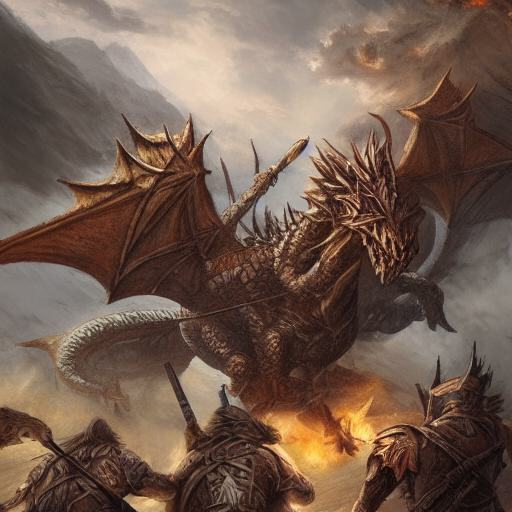
\includegraphics[width=\columnwidth]{introduction/what is a tabletop rpg}
    In tabletop role-playing games like Rise, you play a specific character of your own design.
    Your character can try to do anything you can imagine in a world that the game master, or GM, creates.
    Of course, you won't always succeed.
    The details of your character's capabilities are defined in the pages ahead; when you're done creating a character, it will have a personality of its own, along with strengths, weaknesses, and special abilities.
    Usually, your character will go on adventures with other characters, each of which is played by other players.
    Together, you will create and experience a story with the Game Master, or GM, who defines the universe that the player characters inhabit.

    \subsection{Describing Actions}
        Most of the time, when you're playing a game of Rise, you simply describe what you want your character to do.
        For example, you can say that your character steps out of their room in the inn and walks over to knock on a friend's door.
        Although Rise has rules that could govern some aspects of that scenario, such as an Awareness check to see if your friend notices you knocking, you wouldn't usually reference those rules explicitly.
        Even in the unlikely scenario that your friend doesn't notice you knock the first time, you can just knock again, so there's no point in worrying about the details.
        If something seems reasonable, it probably is, and you don't need to worry about the fiddly bits.

        Sometimes, when you describe what your character tries to do, the action has a narratively relevant chance of failure.
        Instead of knocking on the door to say hi, you might only have time to bang on it once to warn your sleeping friend about an attack from assassins.
        In that case, there's some chance that your friend is sleeping too deeply to notice the noise the first time you knock.
        You could try knocking again, just like in the first scenario, but in this scenario that failure would cost you valuable time to survive the attack.
        In that scenario, you would roll a die to determine whether you succeed in your action - or in this case, whether your friend would succeed in their attempt to notice you.

    \subsection{Using Specific Abilities}
        Instead of describing broadly what you want to have happen, you might choose one of a list of clearly defined abilities that your character can use.
        Every character has specific abilities unique to them, such as a wizard's spells known.
        There are also a number of simple abilities that anyone can use, such as the \ability{dirty trick} or \ability{trip} abilities.
        These universal abilities attempt to adequately describe a wide variety of reasonable improvised actions that you might try to use in combat.

        Explicitly defined abilities have rules for determining what happens when you use them.
        Some abilities, such as attacks in combat, require rolling dice to determine how effective they are.
        Of course, you can use your character's abilities at any time, not just in combat.
        Abilities such as the \spell{create water} or \spell{distant hand} spells can be used to solve other kinds of problems entirely.

    \subsection{Rolling Dice}
        Eventually, you'll have to determine whether something succeeds or fails.
        This can happen as part of using a specific ability that tells you exactly what to roll, or because you tried to narrate your character taking an action that has a dramatically relevant chance of failure.
        In either case, you'll roll a single ten-sided die, also known as 1d10.
        You'll add some modifier that represents how skilled your character is at the particular thing that they are trying to do.
        At the GM's discretion, they may also give the roll an extra bonus or penalty based on the circumstances that your character is in.
        If your die roll is high enough, your character succeeds at whatever they were trying to do.
        Otherwise, your character fails, which may sometimes have additional consequences.

        In Rise, it's entirely possible for characters to be so skilled that they succeed at what they are trying to do even if you roll a 1.
        Likewise, there are tasks that are so obviously impossible for your character that they cannot possibly succeed.
        In those cases, there's no reason to roll!
        Of course, the GM is the final arbiter of whether rolling is necessary.
        They may have information that the players do not.

    \subsection{Why Use So Many Rules?}
        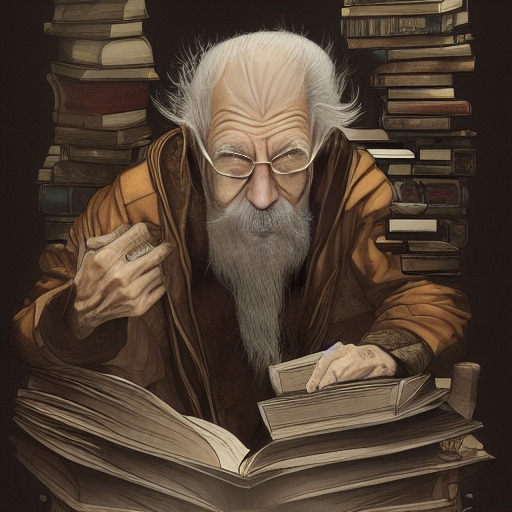
\includegraphics[width=\columnwidth]{introduction/so many rules}

        Tabletop role-playing games attempt to create rules to define how their universe works.
        Some games are intentionally vague or minimalist about their rules, which can be fun!
        Simple games are easy to start playing, and they try to avoid getting in the way of good role-playing.
        However, Rise takes a different approach.
        It spends a lot of effort - and words - attempting to define an internally consistent universe, and creating a large number of specific abilities that can be used in that universe.
        There are a few important advantages to taking this approach: establishing expectations, supporting multiple play styles, and assisting the GM.

        \subsubsection{Establishing Expectations}
            Different people can have very different ideas about what is realistic - or narratively appropriate - in a made-up fantasy universe.
            To some people, kicking in the tavern door and starting a brawl is just some good clean fun, and you'll take a few good punches and then laugh about it later that evening over drinks.
            But to other people, that might sound like a good way to find yourself imprisoned for the foreseeable future with all of your possessions confiscated by the town guard.
            Another interpretation of that scenario might see the brawler seriously injured with a broken bottle in the eye, leaving them partially blinded for weeks - or indefinitely.

            All of those ideas are valid, and they each match the narrative of a particular type of story.
            However, it's important that everyone sitting at a table and playing a game agrees about what to expect.
            Players can get confused or frustrated when their actions have consequences that feel arbitrary or unfair.
            Generally, games are more fun if everyone in the game shares a common set of expectations and conventions.
            Otherwise, games can devolve into disagreements about what is or isn't reasonable.

            One way to establish these expectations is to use a rules system like Rise that defines some expectations explicitly.
            If the scenario above happened in Rise, the last outcome of an incapacitating bottle to the eye shouldn't normally be possible, since the rules explicitly define how injury works.
            Knowing what is and isn't possible can help give players and GMs a useful set of guardrails for what they try to do in the universe.
            It's relatively easy to get everyone to agree about simple things that regular human people have experience with, like how difficult it is to climb a tree.
            However, Rise is full of superhuman people and monsters, and eventually you'll need to figure out how far a barbarian as strong as Hercules can throw a bear.
            Having a single authoritative resource to consult can cut off long disagreements about details that are difficult or impossible to determine objectively.

            Of course, different games played with a flexible rules system like Rise can have very different tones and themes.
            Either of the first two scenarios in the tavern are still plausible in different games, and a GM can use house rules to make vital wounds have more long-term consequences if they want.
            Using a rules system like Rise can help, but it is not the full answer by itself.
            The GM and players always share responsibility for establishing expectations about what genre a game will be, and conforming to those expectations to the extent that it makes the game more fun.

        \subsubsection{Supporting Multiple Play Styles}
            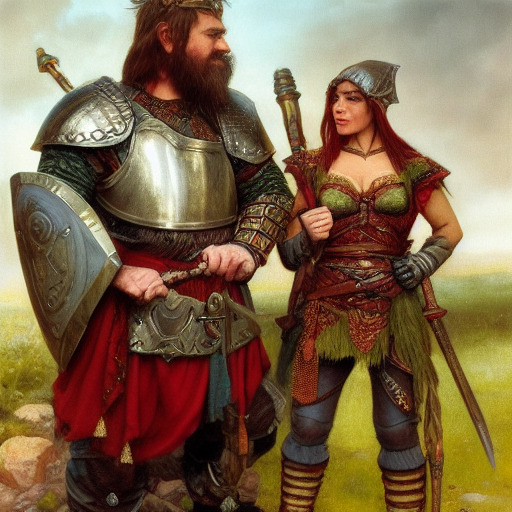
\includegraphics[width=\columnwidth]{introduction/multiple play styles}
            Some people deeply enjoy the process of role-playing itself.
            They enjoy the process of getting into a character and speaking in their voice, exploring their needs and desires, and building a narrative for them over time.
            These people often do not need the confines of a robust rules system, and can play equally well in games with minimal rules or none at all.

            Other people do not enjoy role-playing as an end in itself, or even at all.
            However, they may still enjoy the \textit{game} aspect of a role-playing game.
            Instead of playing a character for their personality and backstory, they may play a character for their unique mechanics and tactical advantages.

            Still other people may be interested in role-playing as a concept, but find it daunting.
            The blank page in front of you when you start painting a picture or writing an essay can be daunting, and that first step is often the hardest to take.
            Giving people a clearly defined set of abilities and specific tools for interacting with the world can enhance creativity by providing a safe space for interaction and experimentation.
            Even if you don't enjoy or feel confident in speaking in your character's voice, you can still engage with the narrative aspects of the adventure by casting a relevant spell or making a relevant skill check.
            People in this middle ground can sometimes enjoy deeper role-playing games while being feeling lost in role-playing games with minimal or nonexistent rules.

            One of the joys - and challenges - of Rise is drawing together people with very different desires and play styles to share a single experience.
            Rules-free role-playing games and tactical wargames can both have a narrower appeal than rules-heavy role-playing games like Rise, which try to provide something for everyone.
            You can run games with deep role-players alongside tactical gamers, and it can be a lot of fun.
            It does place a greater burden on the GM to provide the right ratio of content to keep everyone happy, and it does require the players to be patient when their preferred playstyle is put in the background to support the needs of other players.
            A well-blended game can also draw people out of their comfort zones slowly and safely over time as they observe and start to enjoy the playstyles of the other players in the game.

        \subsubsection{Assisting the GM}
            The Game Master carries an extra weight of responsibility to shape the flow of the game.
            Creating narratively consistent universes, appropriate challenges, and engaging storylines out of thin air is deeply challenging.
            If this job is too difficult, no one will want to do it, and then no one will play the game!
            Making the GM's job easier is a critical component of any role-playing game.

            There are several ways that Rise can make the GM's job easier.
            It provides information about the mechanics and tropes of the universe that the game takes place in, which helps establish expectations and resolve disputes that might come up during the game.
            It will provide a clear narrative foundation for the world and the characters in that world, which minimizes the up-front work required to run a game, once that section of the book is more complete.
            It will provide a wealth of pre-packaged challenges appropriate for players of any power level or play style, and advice for how to use those challenges appropriately, once that section of the book is more complete.
            The GM-focused sections are currently the most unfinished part of Rise, and this will be a more useful guide before Rise is done.

\section{What Makes Rise Different?}
    If you haven't played other tabletop role-playing games, feel free to skip this section.
    If you have, you may wonder what makes Rise unique in a crowded sea of games.
    Rise has five fundamental principles that differentiate it from other TTRPGs: minimal resource management, simultaneous combat, optional complexity, unbounded scaling, and a bounded action economy.

    \subsection{Minimal Resource Management}
        Many games make use of resources like mana, spell slots, or timed cooldowns to limit how often characters can use their abilities.
        These systems have fundamental problems that undercut the fun and flow of a TTRPG, and Rise essentially does not use resources to limit character ability usage.
        In Rise, characters can cast spells or use special attacks any number of times in a row without consuming resources.

        Some systems have resources that are designed to ebb and flow in the course of a typical combat.
        You might expend mana to use a powerful spell, and then regain mana over time by using weaker spells or fulfilling certain conditions.
        Alternately, you might use a spell and then wait some number of in-game turns before you can use that same spell again.
        This can be fiddly to track and hard to recover from if you forget what happened to your resource pool, which is why this approach is more common in video games than in TTRPGs.
        More importantly, this system has no clear way to handle ability usage outside of combat.
        It effectively gives unlimited ability usage when time is no obstacle, but only in an awkward and convoluted way.
        This category of system is unsuitable for Rise because it is too fiddly in combat and doesn't make sense out of combat.

        Some systems have finite-use resources that are tied to the expenditure of in-game time, such as taking long rests, or session breaks.
        You might spend a spell slot to use a powerful spell, and then be unable to cast that spell again until your character rests for some period of time.
        This can be manageable from a complexity perspective if the number of unique resources is small.
        However, it can get dangerously convoluted if characters have a large number of separate or partially interchangeable resource pools, such as using separate pools for individual spell levels.

        The real problem is that this limitation requires you to make your decisions based on not just the current situation, but also on your prediction of all future situations you will encounter before you have the opportunity to rest.
        This contributes significantly to the tactical complexity of deciding each individual action in combat, which slows down the pace of the game.
        It is also punishing to newer players who have less experience with the metagaming required to deduce how many resources an individual fight is worth.
        This strategic complexity is compounded if hit points are treated as an additional resource, since you now have to trade off the potential impact of one limited resource against another limited resource.

        Optimization of resource usage can be unintuitive and out of character, but failure to correctly manage your resources can leave you with no useful abilities remaining.
        This concern can be exacerbated if some characters are extremely resource-intensive while others have no meaningful resources to track.
        No one likes being forced to hide from a difficult fight or take only insignificant actions while your more resource-savvy or resource-independent allies continue using dramatic and powerful abilities.
        It can also add stress to the party dynamics when one character frequently asks for long rests after fights because they expended resources and no one else needs to rest.
        This category of system is unsuitable for Rise because it creates complexity in ways that detract from the fun and narrative of a game instead of adding to it.

        Rise does not use resources to limit normal actions in combat.
        The vast majority of spells, special martial attacks, and other abilities that affect enemies or your environment can be used any number of times.
        There are a small number of abilities with one-round cooldowns, and a universal ability that can only be used once per short rest.
        However, there is no time tracking in the system longer than ``next round''.
        Small cooldowns are a fine-grained balancing tool that allow characters to have powerful abilities which would have detrimental effects for the game if they could be used every turn.

        Rise does use a single universal resource, called ``fatigue'', that recovers based on long rests.
        This allows some opportunity for characters to invest extra effort into specific difficult fights, and to become tired after a long day.
        Normal damage taken during a fight is easily recovered after a ten minute rest.
        This means that you typically don't have to track state between fights.
        However, a GM can prevent that rest time with multiple sequential fights to increase difficulty and drama.

        Overall, Rise uses resource limitations very sparingly.
        This allows it to gain some of their benefits while avoiding the detrimental effects that come from making resource limitations a fundamental part of the system.

    \subsection{Simultaneous Combat}
        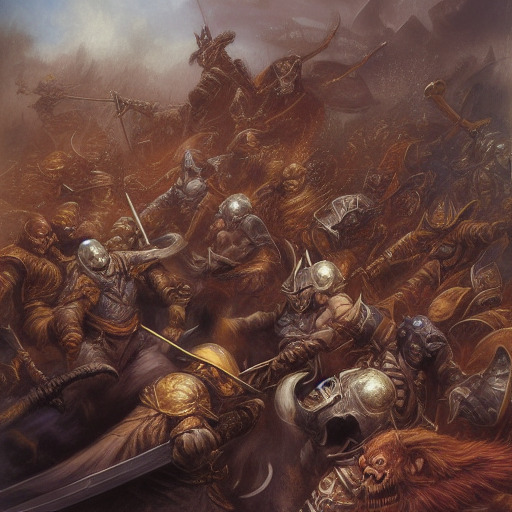
\includegraphics[width=\columnwidth]{introduction/simultaneous combat}
        In most TTRPGs, combat takes place in a series of turns.
        When your turn comes up, you take all of your actions, and then you wait through everyone else's turn until your turn comes again.
        This system has one foundational disadvantage: it is very, very slow.
        Rise uses a simultaneous combat system that dramatically increases the pace of combat.

        Imagine a typical 4-5 player game with 1-2 enemy groups using a traditional turn-based initiative system.
        In this scenario, you have to wait through about 5 turns before it comes back to your turn.
        This number can increase significantly in large-scale fights.
        Each of those 5 or so turns can meaningfully change the battlefield situation on its own by moving, weakening, or defeating various enemies and allies.
        The state of the battlefield at the end of last turn is often drastically different than the state of that battlefield at the start of your new turn.
        Player coordination can be challenging, since they must coordinate in the specific order assigned by the initiative system, and enemy turns can intervene to ruin coordinated plans.

        In theory, every player should accurately track the unfolding battlefield state through each of the intervening turns.
        That would mean everyone would know what to do when their turn comes up.
        In practice, many players find that difficult or impossible.
        Instead, at the start of each of their turns, they ask or try to figure out how the situation has changed.
        Not everyone asks this explicitly, but it must always be analyzed anew.

        Once a player understands the current battlefield state, they can finally decide their actions.
        This typically involves both movement and any number of sequential attacks, so there are many factors to consider.
        Everyone else must wait and do nothing while this happens.
        Once the active player has decided their actions, those actions must be fully rolled and resolved before combat can proceed.
        Even the next player in the initiative order may not be able to make accurate plans during this time, since the die rolls can change those plans.
        All of this combines to make even short combats take an hour or more, and six-person adventuring groups can feel dangerously bloated.

        Rise works differently.
        Combat in Rise is broken up into two phases: the movement phase and the action phase.
        During the movement phase, all creatures move simultaneously, and no attacks are possible.
        Characters can declare certain simple reactive movements like ``stay adjacent to this enemy'' to ensure that they end up in a reasonable position regardless of enemy actions.
        If the movements of characters conflict in impossible ways, initiative checks can temporarily force a linear order of resolution.
        Each player declares their own actions in an arbitrary order as soon as they decide them, so people are not forced to wait and do nothing while slower players contemplate their choices.
        Player coordination is easy, since all actions are happening together.

        During the action phase, players resolve their actions sequentially, but in an arbitrary order of the players' choice.
        This allows slower players to make their decisions when they are ready, while allowing faster players to resolve their actions first.
        Since movement during the action phase is rare, and enemies cannot unexpectedly move, players are typically able to decide their actions much more quickly and easily even when they have a large number of unique abilities to choose from.
        Once all players have resolved their actions, they learn what their enemies did.
        Those actions all resolve simultaneously, so enemy actions cannot interrupt player actions and vice versa.
        Attackers are always responsible for rolling instead of using ``saving throws'' or similar mechanics that force defenders to roll dice.
        All of this means that players can choose and resolve their actions simultaneously and efficiently, minimizing total time spent in combat while still allowing significant tactical complexity.

        The start of each phase still requires a general assessment from all acting players about the current state of the battlefield, which takes just as much time as the assessment in a classic initiative system.
        However, the time required for this tactical analysis only increases marginally as the number of players and enemies in the game increases.
        This allows Rise to handle large player counts or large enemy hordes without becoming glacially slow.
        Combat in Rise flows by quickly, making it much easier to balance time between combat and non-combat encounters within the same game session - or to run through multiple separate, individually challenging combats without sacrificing the pace and energy of the game.

    \subsection{Optional Complexity}
        Many games operate at a consistent level of complexity.
        Many rules-light games are always simple, and many rules-dense games are always complex.
        This is a perfectly reasonable design philosophy.
        Among other benefits, it makes it easy to know what to expect from the game, which helps give the game a well-defined niche.

        Rise is designed to allow players to choose their own level of complexity.
        This broadens its potential audience by allowing people with very different play styles or tolerances for complexity to enjoy the same game together.
        This goal is manifested in several key ways in Rise's design:
        \begin{itemize}
            \item Core gameplay is designed to be simple.
            \item Character creation is deeply interconnected.
            \item Complexity is not tied to narrative roles.
            \item Character power does not require complexity.
        \end{itemize}

        \subsubsection{Simple Core Gameplay}
            The core gameplay loop must be simple.
            You can contribute in combat by relying on one or two standard attacks that you use in all circumstances.
            In narrative situations, you can just roll the skills you have trained, and ignore other options.
            Engaging with the system more deeply than that is a choice, not a requirement.

        \subsubsection{Interconnected Character Creation}
            Character creation and build optimization is a better place to store complexity.
            Creating a Rise character involves a number of decisions, each of which can have nuanced ramifications on other aspects of the system.
            If you are just trying to build a character that matches a desired narrative, you can generally approach each decision in isolation.

            For example, you can decide that your character is intelligent and agile but not very strong or durable, because that is the concept you want.
            That decision has consequences, such as changing how many trained skills you have and what your defenses are.
            If you approach each decision sequentially, each one is relatively easy to make, and doesn't require deep system knowledge.
            On the other hand, trying to mathematically optimize a character requires thinking about many aspects of the system at once.
            This results in a system that is easy to learn but hard to master.

            Even for simple characters, the process of character creation is still one of the most complicated aspects of Rise.
            That is why Rise provides (or will provide, once that section is done) an extensive selection of premade characters for a wide variety of narrative archetypes.
            Each premade character includes advice for how to play that character and level them up.
            The premade characters make the system more accessible to people who don't want to to deal with the complexity of creating a character from scratch.

        \subsubsection{Complexity and Narrative}
            Complexity and simplicity should not be directly connected to a character's concept or narrative.`
            For example, it would be a bad idea to define a system where martial characters are simple and spellcasters are complicated.
            Both of those are rich and evocative narrative constructs.
            Many people who don't enjoy complexity will want to play spellcasters, and many people who enjoy complexity will want to play martial characters.
            Gameplay complexity must be more finely tuned and localized than those sweeping strokes.

            In Rise, gameplay complexity is generally generated by acquiring a large number of increasingly situational abilities.
            Every class has some archetypes that grant additional abilities known and some archetypes that grant additional passive abilities.
            If you like having a lot of unique abilities, you can have a high Intelligence to maximize your insight points, and focus on learning spells and maneuvers that attack your enemies or have situational effects.
            If you like minimizing complexity, you can instead choose archetypes or learn spells that simply grant you passive benefits, and focus on one or two standard attacks that you specialize in.
            Some feats give you new abilities and new circumstances to pay attention to that make you more effective, while others simply increase your passive statistics and defenses.

            Rise specifically handles complexity for martial characters and spellcasters slightly differently.
            Martial characters in Rise typically have fairly simple individual abilities.
            However, they can use those abilities with a variety of meaningfully different weapons.
            A martial character with four unique attacks and three different weapons has twelve different options in combat.
            In addition, martial characters can typically make better use of universal abilities, such as shoving and grappling.

            Spellcasters have more complex and varied individual abilities.
            They also tend to have more abilities that have significant narrative effects.
            However, their abilities are more isolated.
            There is no spellcaster equivalent of martial weapons that would multiply their number of distinct abilities in combat.
            The result of this design is that both martial characters and spellcasters can be very simple or very complicated.
            However, they approach complexity in different ways, ensuring that they feel narratively distinct.

        \subsubsection{Complexity and Power}
            All of this customization of complexity would be mostly pointless if complexity was strongly correlated with character power.
            If exceptionally complicated or hyper-specialized characters were obviously and consistently more effective than other characters, it would push everyone to use those characters.
            Rise structures the tradeoffs between gaining raw power and gaining additional options balanced enough that neither is always superior.

            There will always be some benefit from build optimization and system mastery.
            Players who are deeply familiar with Rise will be able to build characters with more relevant strengths and fewer relevant weaknesses.
            However, the gap between optimized characters and ``normal'' characters is limited.
            There will always be specific contexts where one character's mechanics are superior to another's.
            For example, a specialized defensive melee character may excel in a duel in a confined space.
            However, it may be irrelevant against cavalry archers on an open field.
            Characters in Rise cannot drastically change their capabilities each day, so they will always have moments to shine and moments of weakness.

    \subsection{Unbounded Scaling}
        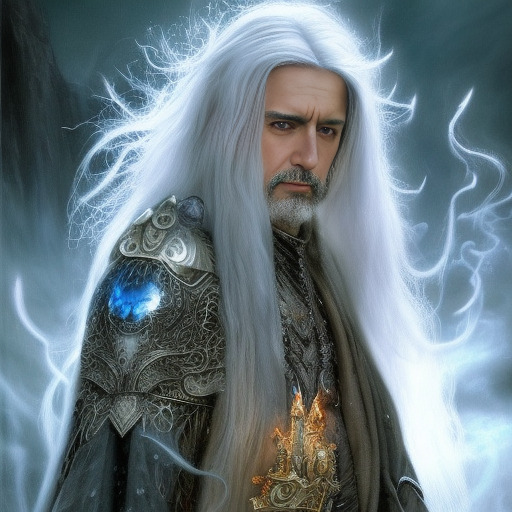
\includegraphics[width=\columnwidth]{introduction/unbounded scaling}
        Some systems uses bounded bonuses for accuracy or other game statistics.
        Bounded scaling means that every character of the same power level - or in some systems, of any power level - has a similar chance of success with any given skill check or attack roll.
        This can frequently cause narratively inappropriate and even comical events, and Rise explicitly rejects this philosophy.

        Imagine a typical party of four players, with one character being exceptionally skilled at a particular task.
        Perhaps the rogue is exceptionally skilled at lying, or a barbarian is exceptionally skilled at climbing.
        If ``exceptionally skilled'' only means that they have a \plus5 bonus on a d20 compared to \plus0 from the rest of the party, the exceptionally skilled character will only get the best result in the party half the time.
        The other half of the time, some other character with no relevant skills will meet or exceed the skilled character's result - sometimes by a dramatic margin.
        When failure compared to rank amateurs happens this often, it becomes hard to take seriously the idea that any character can be exceptionally skilled at anything.

        Rise characters can have dramatic statistical differences between each other, even at low levels.
        It uses a d10 as the fundamental die, which makes every bonus more significant.
        In addition, a 1st-level character can easily reach a \plus6 bonus with a skill check that is particularly relevant to their character.
        This means that a skilled character can beat a party of rank amateurs 80\% of the time, and at higher levels their success becomes completely guaranteed.
        Likewise, the difference in Mental defense between a powerful sorcerer and a cowardly rogue can allow mind-affecting attacks to almost always hit a rogue while almost never hitting the sorcerer.
        These statistical differences do not always grow with level, but they remain significant at every level.

        One advantage of systems with bounded scaling is that it is easier to guarantee that every character is relevant in any situation.
        Even if your character has no useful abilities of any kind, you might sometimes succeed on important actions through sheer luck.
        However, this design philosophy often breaks the symmetry between magical and non-magical characters.
        Magical characters can often use extremely specific and powerful abilities that are impossible for nonmagical characters to duplicate.
        If magical characters also have similar odds of success with all generic mechanics of the game, they will almost certainly have far more influence over the narrative of the game than any nonmagical character can hope to match.

        The philosophy of Rise is that it's okay for some characters to be irrelevant in specific contexts.
        It's good to give people time in the spotlight where their character's abilities help solve the specific problem that the group is facing when no other character could.
        Rise encourages that, and makes it impossible for one character to be relevant in \textit{all} contexts.
        Each character has their own strengths and weaknesses, and if you try to be good at everything, you'll fall behind people who specialize in a particular area.
        This will naturally rotate the spotlight between different characters, allowing each player to feel relevant and important in turn.

        This dramatic scaling is also used to govern the power of characters over time, in addition to the power of characters relative to each other.
        Rise attempts to model a massive power range for player characters.
        They are expected to start their journeys at level 1 as little more than commoners, and by level 21 they are effectively demigods who can alter the fate of entire worlds.
        This is a critical part of the narrative fabric of Rise, and it is reflected in the statistics and abilities of characters.
        If a level 1 kobold posed even a tiny threat to a level 21 character, the mechanics of the game would sabotage the purported narrative of power and growth.
        In Rise, overall character power doubles approximately every two to three levels.
        The system takes some care to avoid bloating numbers to unwieldy levels on this journey, and the use of the d10 as the standard die helps immensely.

    \subsection{Bounded Action Economy}
        It is dangerous to to give characters too many actions each turn.
        Each additional action a character can take increases how difficult it is for a player to decide what to do on their turn.
        In addition, each additional action increases the complexity of the change between the start of the turn and the end of the turn.
        This is especially risky with Rise's simultaneous initiative system, which combines the actions taken by all characters into a single resolution process.

        Rise places significant limitations on how many relevant actions each character can take on their turn.
        Generally, characters can only move during the movement phase and then take one significant action each turn.
        Some characters can use a minor action to accomplish something useful.
        However, that essentially marks the end of action economy scaling, even up to the maximum level.

        Detrimental effects that could deny actions are also heavily limited.
        Total action denial effects are only usable by high level characters, and even then they only work against weak enemies or enemies that have already been significantly damaged.
        Taking actions is fun, and sitting quietly while everyone else does things can be very frustrating.
        Similarly, completely removing an enemy's ability to act can easily remove the tension from a fight before it's actually over.


\chapter{Core Mechanics}

This chapter describes the core mechanics of Rise.
It defines how attributes work and explains how to make physical attacks in combat.

\section{Attacks and Checks}\label{Attacks and Checks}
    You can take many actions without needing to roll a die at all.
    However, eventually you will need to do something where there is a dramatically significant chance of failure.
    In that case, you will need to roll a die to see if you succeed or fail.
    Almost all rolls you will need to make can be described as an \glossterm{attack roll} or a \glossterm{check}.

    \subsection{Attack Rolls}
        Attack rolls are required to make \glossterm{attacks}.
        Anything that affects another creature in a potentially harmful way, such as striking a creature with a sword, is an attack.
        Many abilities are always considered attacks, even if you use them in a way that you believe is not harmful.

        To make an attack roll, roll 1d10 and add your \glossterm{accuracy} with the attack.
        The sum of your die roll and your accuracy is called your \glossterm{attack result}.
        You compare your attack result to a \glossterm{defense} that your \glossterm{target} has (see \pcref{Defenses}).
        All attacks specify which defense they are compared to.
        If your result is at least equal to your target's defense, the attack succeeds.
        This almost always means the target suffers some harmful effect, such as taking \glossterm{damage}.
        Otherwise, the attack fails.

        \subsubsection{Exploding Attacks}\label{Exploding Attacks}
            When you make an attack roll, if you roll a 10 on the d10, the die ``explodes''.
            You roll again and add the second result to the original 10 before applying your \glossterm{accuracy}.
            If you roll a 10 on the extra roll, you keep rolling until you stop rolling a 10 and add all of the rolls together.

        \subsubsection{Critical Hit}\label{Critical Hit}
            If your attack result is at least 10 higher than your target's defense, your attack is a \glossterm{critical hit}.
            Many attacks have special effects on critical hits.
            Unless its critical hit effects are otherwise noted, any attack that deals damage deals double that damage on a critical hit.

    \subsection{Checks}\label{Checks}
        Checks are required to perform actions that have a chance of failure that are not attacks.
        For example, climbing a wall or remembering an obscure piece of trivia may require a check.

        To make a check, roll 1d10 and add your \glossterm{check modifier} with the check.
        You compare the die result, including your check modifier, to a \glossterm{difficulty rating} (DR) that represents the difficulty of the task.
        The more difficult the task, the higher the DR will be.
        If your result is at least equal to the DR, the check succeeds.
        This usually means you accomplish a task successfully.
        Normal Difficulty Ratings are described in \tref{Difficulty Ratings}.

        \begin{dtable}
            \lcaption{Difficulty Ratings}
            \begin{dtabularx}{\columnwidth}{p{8em} X}
                \tb{Difficulty (DR)} & \tb{Example (Skill Used)} \\
                \bottomrule
                Trivial (0)      & Hear a coversation from 10 feet away (Awareness)                          \\
                Average (5)      & Tie or untie a typical knot (Devices)                                     \\
                Tough (10)       & Swim in rough water (Swim)                                                \\
                Challenging (15) & Balance on a one-inch wide wood beam (Acrobatics)                         \\
                Heroic (20)      & Open a high quality lock (Devices)                                        \\
                Legendary (25)   & Leap across a 30-foot chasm with a running start (Jump)                   \\
                Epic (30)        & Convince a wise mayor her husband is secretly a werewolf (Persuasion)     \\
                Godlike (40)     & Track three orcs across firm ground after 24 hours of rainfall (Survival) \\
            \end{dtabularx}
        \end{dtable}

        \subsubsection{Critical Success}
            If your check result is at least 10 higher than the DR, your check is a \glossterm{critical success}.
            Some checks have a special effect on a critical success.
            For example, a critical success while climbing means you move twice as quickly (see \pcref{Climb}).

        \subsubsection{Critical Failure}
            If your check result is at least 10 lower than the DR, your check is a \glossterm{critical failure}.
            Some checks have a special effect on a critical failure, which is usually bad for the character making the check.
            For example, a critical failure while climbing means you fall (see \pcref{Climb}).

\section{Combat Time}\label{Combat Time}
    The world of Rise can be a harsh one, and not all disagreements can be resolved peacefully.
    At some point, you will be forced to enter combat.
    This section explains how time passes in combat.

    \subsection{Rounds}\label{Rounds}

        Combat takes place in a series of \glossterm{rounds}, which represent about six seconds of time.
        Each round of a combat is divided into three \glossterm{phases} (see \pcref{Phases}).
        After all phases are complete, the round ends and the next round begins.

    \subsection{Actions}\label{Actions}

        You can take \glossterm{actions} in combat to defeat your foes.
        There are four types of actions: \glossterm{standard actions}, \glossterm{minor actions}, \glossterm{move actions}, and \glossterm{free actions}.
        % TODO: define conflicting action limits (drawing a sword and sheathing a shield?)

        \subsubsection{Standard Actions}\label{Standard Actions}
            Most common activities require a \glossterm{standard action}, such as attacking with a weapon, casting a spell, and using many special abilities.
            Using a standard action generally takes about three seconds of time within the game, and it requires most of your attention during that time.

            You can take one standard action per round.

        \subsubsection{Minor Actions}\label{Minor Actions}
            Some special abilities require a \glossterm{minor action}.
            Using a minor action does not take much time or attention, and it can be done at the same time as any other actions.

            You can normally take one minor action per round.
            However, you can choose to take an additional minor action in place of a \glossterm{standard action}.

        \subsubsection{Move Actions}\label{Move Actions}
            You can move around a battlefield as a \glossterm{move action}.
            Using a move action generally takes about three seconds of time within the game, and it requires most of your attention during that time.

            You can normally take one move action per round.
            However, you can choose to take an additional move action in place of a \glossterm{standard action}.

        \subsubsection{Free Actions}\label{Free Actions}
            Many minor activities require a \glossterm{free action}, such as drawing or sheathing a weapon.
            Using a free action does not take much time or attention, and it can be done at the same time as any other actions.

            You can take any number of free actions per round.

    \subsection{Phases}\label{Phases}

        There are three \glossterm{phases} in each round: a \glossterm{movement phase}, an \glossterm{action phase}, and sometimes a \glossterm{delayed action phase}.
        Each phase specifies the types of actions that can be taken during that phase.
        As a special case, \glossterm{free actions} may be taken during any phase.

        \subsubsection{The Movement Phase}\label{The Movement Phase}
            During the \glossterm{movement phase}, you can take one \glossterm{move action}.
            The most common move action is the \textit{hustle} ability, which allows you to move a distance equal to your \glossterm{speed}.
            For details, see \pcref{Movement and Positioning}.

        \subsubsection{The Action Phase}\label{The Action Phase}
            During the \glossterm{action phase}, you can take one \glossterm{minor action} and one \glossterm{standard action}.
            Alternately, you can take a \glossterm{move action} or additional \glossterm{minor action} in place of your standard action.
            Most of the time, you will simply take a single standard action.

        \subsubsection{The Delayed Action Phase}\label{The Delayed Action Phase}
            During the \glossterm{delayed action phase}, you can take a \glossterm{minor action} or \glossterm{standard action} if you did not use the corresponding action in the \glossterm{action phase}.
            Alternately, you can take a \glossterm{move action} or additional \glossterm{minor action} in place of a standard action.
            In addition, some abilities have effects during the delayed action phase instead of or in addition to their effects in the action phase.
            For example, \glossterm{spells} normally have no effect during the action phase, and have their full effect during the delayed action phase.

    \subsection{Resolving Actions}\label{Resolving Actions}

        Within each phase, actions of all creatures are simultaneously resolved in the following order.
        Allies with the ability to communicate can freely coordinate their actions with each other, within reasonable limits.

        \begin{enumerate*}
            \item Choose actions.
            \item Determine targets affected by actions.
            \item Apply the results of \glossterm{swift abilities}.
            \item Check action success.
                Example: Making attack rolls.
            \item Determine action results.
                Example: Making damage rolls.
            \item Apply action results.
                Examples: Reducing hit points, moving creature locations, and applying penalties.
                % Effects that trigger when damage is dealt, such as Concentration checks (see \pcref{Concentration}), are resolved now.
        \end{enumerate*}

        In the vast majority of cases, there is no need to go through this order explicitly.
        Combats will run much faster if attack and damage rolls are generally made and announced at the same time as those actions are chosen, even before all characters have explicitly stated their actions.
        The order of resolution matters when creatures take actions that directly conflict with each other.

        \subsubsection{Swift Abilities}\label{Swift Abilities}
            Some abilities resolve before other actions in the same phase.
            These abilities have the \glossterm{Swift} tag.
            They resolve after targets are determined, but before attack rolls are made.
            Swift abilities never require attack rolls, and almost always affect only the creature using the ability.

            For example, the \textit{total defense} ability is a swift ability.
            It increases your defenses against attacks made during the same phase (see \pcref{Total Defense}).

        \subsubsection{Delayed Abilities}\label{Delayed Abilities}
            Some abilities resolve a full phase after they were originally used.
            These abilities have the \glossterm{Delayed} tag.
            For example, all \glossterm{spells} have the \glossterm{Delayed} tag.
            Abilities with this tag cannot be used during the \glossterm{delayed action phase}.

            During the \glossterm{action phase}, creatures using delayed abilities do not choose targets or take any later steps in resolving the abilities.
            The abilities finish resolving during the delayed action phase, allowing creatures to choose targets, make attack rolls, and so on.

            You must still make all choices required to use a delayed ability when you first use the ability during the action phase.
            For example, when casting a spell, you must choose which spell (or \glossterm{subspell}) you cast, and any \glossterm{augments} you apply to that spell, during the action phase.

        \subsubsection{Conflicting Actions}\label{Conflicting Actions}

            Sometimes, actions that occur at the same time can conflict with each other.
            In this case, each involved character rolls an \glossterm{initiative} check (see \pcref{Initiative}).
            The creature with the highest check result succeeds.
            All other creatures come as close as possible to completing their intended action.

            For example, if two creatures were racing to reach a door, they would both roll initiative.
            The winner would reach the door and stop in their intended square, and the loser would stop as close as possible to their intended square.

\section{Character Statistics}
    This section explains how character statistics, such as how strong you are or how accurate your attacks are, should be calculated.

    \subsection{Attributes}\label{Attributes}

        Each character has six \glossterm{attributes}: Strength (Str), Dexterity (Dex), Constitution (Con), Intelligence (Int), Perception (Per), and Willpower (Wil).
        Each attribute represents a character's raw talent in that area.
        A 0 in an attribute represents average human capacity.
        That doesn't mean that every commoner has a 0 in every attribute; not everyone is average, after all.

        \subsubsection{Strength (Str)}\label{Strength}
            Strength measures muscle and physical power.
            It has the following effects:
            \begin{itemize}
                \item Strength determines how much a character can carry (see \tref{Carrying Capacity by Strength}).
                \item Strength affects Strength-based skills: Climb, Jump, and Swim (see \pcref{Skills}).
                \item If your Strength is negative, you take a penalty to all Strength-based skills equal to your Strength.
                \item If your Strength is negative, you take a penalty to \glossterm{strike damage} equal to half your Strength in \glossterm{die increments}.
            \end{itemize}

            If you have a high Strength, you can use it to determine several statistics:
            \begin{itemize}
                \item Your \glossterm{strike damage} (see \pcref{Strike Damage}).
                \item Your \glossterm{threat} (see \pcref{Threat}).
                \item Your Fortitude defense (see \pcref{Defenses}).
            \end{itemize}

        \subsubsection{Dexterity (Dex)}\label{Dexterity}
            Dexterity measures hand-eye coordination, agility, and reflexes.
            It has the following effects:
            \begin{itemize}
                \item Dexterity affects Dexterity-based skills: Acrobatics, Escape Artist, Ride, Sleight of Hand, and Stealth (see \pcref{Skills}).
                \item You gain a bonus (or penalty) to your Reflex defense equal to your starting Dexterity.
                \item If your Dexterity is negative, you take a penalty to all Dexterity-based skills equal to your Dexterity.
            \end{itemize}

            If you have a high Dexterity, you can use it to determine several statistics:
            \begin{itemize}
                \item Your \glossterm{accuracy} with \glossterm{physical attacks} using light melee and thrown weapons (see \pcref{Physical Accuracy}).
                \item Your Armor and Reflex defenses (see \pcref{Defenses}).
            \end{itemize}

        \subsubsection{Constitution (Con)}\label{Constitution}
            Constitution represents your health and stamina.
            It has the following efects:
            \begin{itemize}
                \item You gain bonus hit points based on your starting Constitution (see \pcref{Hit Points}).
                \item You heal additional hit points when you take a \glossterm{short rest} based on your starting Constitution (see \pcref{Short Rest}).
                \item You gain a bonus (or penalty) to your Fortitude defense equal to your starting Constitution.
                \item You reduce your \textit{encumbrance} for weight or heavy armor by an amount equal to your starting Constitution.
            \end{itemize}

            If you have a high Constitution, you can use it to determine your Fortitude defense (see \pcref{Defenses}).

        \subsubsection{Intelligence (Int)}\label{Intelligence}
            Intelligence represents how well you learn and reason.
            It has the following effects:

            \begin{itemize}
                \item You gain bonus languages equal to your starting Intelligence (see \pcref{Languages}).
                \item You gain extra skill points equal to twice your starting Intelligence (see \pcref{Skill Points}).
                \item Your Intelligence affects Intelligence-based skills: Craft, Deduction, Disguise, Heal, Knowledge, and Linguistics (see \pcref{Skills}).
                \item If your starting Intelligence is negative, you lose skill points equal to twice your starting Intelligence.
                \item If your Intelligence is negative, you take a penalty to all Intelligence-based skills equal to your Intelligence.
            \end{itemize}

            If you have a high Intelligence, you can use it to determine your Mental defense (see \pcref{Defenses}).

            \par An animal has an Intelligence score of \minus6 or lower.
            A creature of humanlike intelligence has a score of at least a \minus5 Intelligence.

        \subsubsection{Perception (Per)}\label{Perception}
            Perception describes your ability to observe and be aware of your surroundings.
            It has the following effects:
            \begin{itemize}
                \item Your Perception affects Perception-based skills: Awareness, Creature Handling, Sense Motive, Spellcraft, and Survival (see \pcref{Skills}).
                \item If your Perception is negative, you take a penalty to all Perception-based skills equal to your Perception.
                \item If your Perception is negative, you take a penalty to accuracy with all attacks equal to half your Perception.
            \end{itemize}

            If you have a high Perception, you can use it to determine several statistics:
            \begin{itemize}
                \item Your \glossterm{accuracy} with \glossterm{physical attacks} (see \pcref{Physical Accuracy}).
                \item Your Reflex defense (see \pcref{Defenses}).
            \end{itemize}

        \subsubsection{Willpower (Wil)}\label{Willpower}
            Willpower represents your ability to endure mental hardships.
            It has the following effects:
            \begin{itemize}
                \item You gain a bonus (or penalty) to the number of \glossterm{action points} you have equal to your starting Willpower.
                \item You gain a bonus (or penalty) to your Mental defense equal to your starting Willpower.
            \end{itemize}

            If you have a high Willpower, you can use it to determine your Mental defense (see \pcref{Defenses}).

    \subsection{Accuracy}\label{Accuracy}
        Your accuracy with an \glossterm{attack} is the number that you add to the \glossterm{attack roll}.
        You will have multiple different attacks you can make.
        The accuracy for an attack depends on the type of attack it is.

        \subsubsection{Physical Accuracy}\label{Physical Accuracy}
            Your accuracy with a \glossterm{physical attack}, such as a \glossterm{strike}, is normally equal to the higher of your level and your Perception.
            If you are using a \glossterm{light weapon}, you may use your Dexterity instead.
            In addition to this base number, your accuracy can include any number of bonuses and penalties from other sources.

            \parhead{Proficiency} Each creature is \glossterm{proficient} with a number of weapons.
            For details about the weapons you can be proficient with, see \pcref{Weapons}.
            Your proficiencies are primarily determined by your class, but some abilities also grant proficiency with additional weapons.
            If you make a \glossterm{physical attack} with a weapon you are not proficient with, you take a \minus2 penalty to accuracy.

    \subsection{Damage}\label{Damage}
        Some attacks deal damage when they hit.
        Damage does not represent serious physical injury to your body.
        Instead, it represents a depletion of some combination of endurance, luck, or even divine providence that prevents you from suffering more serious injury
        When you take damage, you reduce your \glossterm{hit points} by that amount (see \pcref{Hit Points}).
        If you have no hit points remaining, you may take that damage as \glossterm{vital damage} instead, which represents potentially life-threatening injuries (see \pcref{Vital Damage}).

        Most attacks deal damage equal to the result rolled from a pool of dice.

        \subsubsection{Die Increments}\label{Die Increments}
            Many abilities can increase or decrease your damage with abilities.
            These modifiers always increase or decrease your damage by one \glossterm{die increment}.
            Increasing by one die increment is written as \plus1d, and decreasing by one die increment is written as \minus1d.
            A set of damage dice can increase in size in \glossterm{die increments}.
            Damage dice change in size using the following pattern:
            \begin{itemize}
                \item 1 damage (minimum)
                \item 1d2
                \item 1d3
                \item 1d4
                \item 1d6
                \item 1d8
                \item 1d10
                \item 2d6
                \item 2d8
                \item 2d10
                \item 4d6
                \item 4d8
                \item 4d10
                \item 5d10
                \item 6d10
            \end{itemize}

            For each die increment that increases the damage, move one space down the list.
            Likewise, for each die increment that decreases the damage, move one space up the list.
            After the damage dice reach 4d10, each additional die increment simply adds an extra 1d10 of damage.

        \subsubsection{Standard Damage}\label{Standard Damage}
            Most damaging effects use \glossterm{standard damage} as a baseline to determine the damage they deal.
            Your \glossterm{standard damage} with an ability is based on that ability's \glossterm{power}, if it has one (see \pcref{Power}).
            Otherwise, it is based on your level.
            In either case, it starts at 1d8 and increases by \plus1d per two power or per two levels.
            This is summarized on \trefnp{Standard Damage}.

        \begin{dtable}
            \lcaption{Standard Damage}
            \begin{dtabularx}{\columnwidth}{l X}
                \tb{Power} & \tb{Damage} \\
                0--1   & 1d8  \\
                2--3   & 1d10 \\
                4--5   & 2d6  \\
                6--7   & 2d8  \\
                8--9   & 2d10 \\
                10--11 & 4d6  \\
                12--13 & 4d8  \\
                14--15 & 4d10 \\
                16--17 & 5d10 \\
                18--19 & 6d10 \\
                20--21 & 7d10 \\
                22--23 & 8d10 \\
                24--25\fn{1} & 9d10 \\
            \end{dtabularx}
            1. For values above 25, increase by 1d10 at every even value.
        \end{dtable}

        \subsubsection{Strike Damage}\label{Strike Damage}
            The damage you deal with a single \glossterm{strike} from a weapon is called your \glossterm{strike damage}.
            Your base \glossterm{strike damage} is equal to \glossterm{standard damage} based on your level or your Strength, whichever is higher.
            For example, if you have a Strength of 4, your base \glossterm{strike damage} would be equal to 2d6 (1d8 \plus2d).
            When you make a strike with a weapon, you also apply that weapon's damage modifier, if any.
            Some abilities other than \glossterm{strikes} deal damage based on your \glossterm{strike damage}.

            \parhead{Creature Size and Damage}\label{Creature Size and Damage}
            Larger creatures deal more damage with their weapons.
            Each creature size above Medium grants a \plus1d bonus to \glossterm{strike damage}.
            Likewise, each creature size below Medium imposes a \minus1d penalty to damage with strikes.
            This is described in \tref{Size in Combat}.

    \subsection{Defenses}\label{Defenses}
        Usually, when you are attacked, the attacker has to make an \glossterm{attack roll} against a specific defense.
        If the attack roll is at least as high as that defense, the attack succeeds.
        \begin{itemize}
            \item Armor defense (AD): Your Armor defense protects you from normal physical attacks, such as attempts to hit you with a sword.
                It is the most commonly used defense.
            \item Reflex defense: Your Reflex protects you from attacks you have to avoid, such as explosions or falling rocks.
            \item Fortitude defense: Your Fortitude defense protects you from attacks you have to physically endure or resist, such as poisons and deadly spells.
            \item Mental defense: Your Mental defense protects you from attacks you have to mentally endure or resist, such as terrifying creatures and magical manipulation.
        \end{itemize}

        \subsubsection{Defense Values}\label{Defense Values}

            Each of your defenses is calculated in the following way:

            \begin{figure}[h]
                \centering Level or defense attribute \add class defense bonus \add other bonuses and penalties
            \end{figure}

            The attributes and relevant bonuses which apply to each defense are described in \trefnp{Defense Calculations}.

            \begin{dtable!*}
                \lcaption{Defense Calculations}
                \begin{dtabularx}{\textwidth}{l l l l >{\lcol}X}
                    \tb{Defense Name} & \tb{Attributes} & \tb{Starting Attribute Modifier} & \tb{Body Armor Modifier} & \tb{Shield Modifier} \\
                    \midrule
                    Armor defense     & Dex & \tdash & Yes & Yes \\
                    Fortitude defense & Con or Str & Con & No  & No  \\
                    Reflex defense    & Dex or Per & Dex & No  & Yes \\
                    Mental defense    & Wil or Int & Wil & No  & No  \\
                \end{dtabularx}
            \end{dtable!*}

            \parhead{Class Bonuses} Each class provides bonuses to some combination of Fortitude, Reflex, and Mental defense.
            \parhead{Natural Armor} Creatures with unusually tough skin or thick hide, including most monsters, gain bonuses to their Armor defense.
            These bonuses stack with any armor such creatures might wear.
            \parhead{Size Modifier} Large creatures have a penalty to Reflex defense.
            For details, see \tref{Size in Combat}.

        \subsubsection{Resisting Attacks}
            If an attack fails against you, you almost always suffer no effects from the attack.
            Even if the attack had no obvious physical or visual effects, a creature that resists an attack still feels a hostile force or a tingle, but cannot usually deduce the exact nature of the attack.
            The Spellcraft skill can be used to learn about failed \glossterm{magical} attacks against you (see \pcref{Spellcraft}).

            \parhead{Lowering Defenses} Whenever you are subject to an attack that you are aware of, you can voluntarily lower your defenses against the attack.
            If you do, your defense is treated as 0 against the attack.

    \subsection{Initiative}\label{Initiative}
        When multiple creatures take mutually impossible actions simultaneously, such as racing to be the first one to a door, they must roll initiative checks.
        For details, see \pcref{Conflicting Actions}.
        Your bonus on \glossterm{initiative} checks is normally equal to your Dexterity or Perception, whichever is higher.

        \parhead{Movement-Based Initiative}\label{Movement-Based Initiative}
        When making \glossterm{initiative} checks to determine the success of movement, having a faster movement speed is helpful (see \pcref{Movement and Positioning}).
        For every 5 feet of movement you would have available after completing your movement, you gain a \plus2 bonus to any initiative checks necessary to determine whether your movement succeeds.
        Regardless of whether your initiative check succeeds or fails, you cannot use that ``excess'' movement to move after making such an initiative check.

    \subsection{Threat}\label{Threat}
        Each creature has a value that represents how threatening it is.
        This value is called a creature's \glossterm{threat}.
        Many monsters choose the targets of their attacks based on the threat of their foes.
        Your base threat is equal to the higher of your level and your Strength.
        In addition, you gain bonuses to your threat based on your equipment and some other effects which can make you appear more or less intimidating.

        \subsection{Threat From Equipment}
            If you are visibly wearing \glossterm{body armor}, you gain a bonus to your threat equal to half the defense bonus provided by the armor.
            For this purpose, ignore any abilities that increase the defense bonus you gain from the armor, and only use the base defense bonus from the armor itself.
            If you are visibly wielding a weapon or otherwise obviously capable of inflicting lethal damage, you gain a \plus2 bonus to your threat.

        \subsection{Threat From Size}
            You gain a \plus2 bonus to your threat for each size category that you are larger than Medium.
            Likewise, you take a \minus2 penalty to your threat for each size category that you are smaller than Medium.

        \subsection{Subjective Threat Modifiers}
            In addition to your base \glossterm{threat}, some actions and abilities modify the threat that particular creatures perceive you have.
            The most common threat modifier comes from dealing damage.
            Whenever you deal damage, you gain a \plus2 bonus to threat until the end of the next round against all creatures that know you dealt that damage.

            Some abilities can also increase or decrease your threat against particular creatures.
            For example, the \textit{Conceal Threat} ability from the Bluff skill allows you to lower your apparent threat to creatures that fail to see through the deception (see \pcref{Conceal Threat}).

        \subsection{Consistent Targeting}
            Unless their descriptions state otherwise, monsters prefer to keep attacking the same target rather than changing targets frequently.
            A monster will only change targets based on \glossterm{threat} if the new target has a threat at least 5 points closer to its preference than its current target.

        \subsection{Threat While Incapacitated}
            While you are unconscious or otherwise obviously unable to take hostile actions, you take a \minus10 penalty to threat.
            Many creatures stop attacking unconscious creatures, preferring to focus on targets that can still cause harm.
            It is possible to trick creatures into thinking you are not a threat by playing dead or using similar tactics.

    \subsection{Size in Combat}\label{Size in Combat}
        Size affects your \glossterm{space} and \glossterm{reach} in combat, your Reflex defense, your \glossterm{strike damage}, and how easily you overwhelm creatures and are overwhelmed yourself.
        These effects are shown on \trefnp{Size in Combat}.

        \begin{dtable*}
            \lcaption{Size in Combat}
            \begin{dtabularx}{\textwidth}{l l l l p{4em} p{4.5em} p{3em} p{5.5em} X}
                \tb{Size} & \tb{Space}\fn{1} & \tb{Reach}\fn{1} & \tb{Base Speed} & \tb{Reflex Modifier} & \tb{Damage Modifier}\fn{2} & \tb{Overwhelm Value}\fn{3} & \tb{Overwhelm Resistance}\fn{4} & \tb{Example Creature} \\
                \bottomrule
                Fine              & 1/2 ft.    & 0          & 10 ft. & \plus8  & \minus4d & 1/4 & \tdash & Fly                      \\
                Diminutive        & 1 ft.      & 0          & 15 ft. & \plus6  & \minus3d & 1/2 & \tdash & Toad                     \\
                Tiny              & 2-1/2 ft.  & 0          & 20 ft. & \plus4  & \minus2d & 1/2 & \tdash & Cat                      \\
                Small             & 5 ft.      & 5 ft.      & 25 ft. & \plus2  & \minus1d & 1 & \tdash & Halfling                 \\
                Medium            & 5 ft.      & 5 ft.      & 30 ft. & \tdash  & \tdash   & 1 & \tdash & Human                    \\
                Large (tall)      & 10 ft.     & 10 ft.     & 40 ft. & \minus2 & \plus1d  & 2 & 1 & Ogre                     \\
                Large (long)      & 10 ft.     & 5 ft.      & 40 ft. & \minus2 & \plus1d  & 2 & 1 & Horse                    \\
                Huge (tall)       & 15 ft.     & 15 ft.     & 50 ft. & \minus4 & \plus2d  & 3 & 2 & Cloud giant              \\
                Huge (long)       & 15 ft.     & 10 ft.     & 50 ft. & \minus4 & \plus2d  & 3 & 2 & Bulette                  \\
                Gargantuan (tall) & 20 ft.     & 20 ft.     & 60 ft. & \minus6 & \plus3d  & 4 & 3 & 50-ft.\ animated statue  \\
                Gargantuan (long) & 20 ft.     & 15 ft.     & 60 ft. & \minus6 & \plus3d  & 4 & 3 & Kraken                   \\
                Colossal (tall)   & 25\add ft. & 25\add ft. & 70 ft. & \minus8 & \plus4d  & 5 & 4 & Colossal animated object \\
                Colossal (long)   & 25\add ft. & 25\add ft. & 70 ft. & \minus8 & \plus4d  & 5 & 4 & Great wyrm red dragon    \\
            \end{dtabularx}
            1 Creatures can vary in space and reach.  These are simply typical values.  \\
            2. This modifier applies to \glossterm{strike damage}. \\
            3. See \pcref{Overwhelm Value}. \\
            4. See \pcref{Overwhelm Resistance}. \\
        \end{dtable*}

        \subsubsection{Space}\label{Space}
            A creature's \glossterm{space} is the area its body occupies while fighting.
            All humanoid races take up a 5-ft.\ by 5-ft.\ space in combat, which is a single \glossterm{square}.
            Normally, other creatures can't be in the space you occupy.
            Most creatures have a space significantly larger than the physical space their body occupies because they need room to maneuver in combat.

        \subsubsection{Reach}\label{Reach}
            A creature's \glossterm{reach} is the distance that its \glossterm{melee} attacks can reach.
            Enemies within a creature's reach are considered \glossterm{threatened}.

        \subsubsection{Base Speed}\label{Base Speed}
            A creature's \glossterm{base speed} is the distance that it can usually move.
            In addition to a base speed, most creatures have specific \glossterm{movement modes} that allow them to move in particular ways.
            The most common movement mode is a \glossterm{land speed}, which allows creatures to move across the ground.
            Most creatures, including all humanoid races, have a land speed equal to their base speed.
            There are other movement modes that can allow creatures to move in different ways.
            For example, most birds have a \glossterm{fly speed}, which allows them to move through the air.
            For details about other speeds, see \pcref{Movement Modes}.

        \subsubsection{Other Effects}
            A creature's size affects a number of additional skills and abilities.
            For example, larger creatures have a penalty to Stealth checks (see \pcref{Size and Stealth}).
            The effects of unusual size are described in those skills and abilities.
            Unusually large or small creatures also have other special rules apply to them, as described below.

        \subsubsection{Very Small Creatures}
            \parhead{Space} If a creature takes up less than a single square of space, you can fit multiple creatures in that square. You can fit four Tiny creatures in a square, twenty-five Diminuitive creatures, or 100 Fine creatures.

            \parhead{Reach} Creatures that take up less than 1 square of space typically have a natural reach of 0 feet, meaning they can't reach into adjacent squares. They must enter an opponent's square to attack in melee. You can attack into your own square if you need to, so you can attack such creatures normally. Since they have no natural reach, they do not threaten the squares around them.

            If a creature without a natural reach uses a reach weapon, it gains no benefits or penalties (see \pcref{Reach Weapon}).

            \parhead{Movement} Creatures three size categories smaller than you are not considered obstacles and do not hinder your movement.

        \subsubsection{Very Large Creatures}
            \parhead{Space} Very large creatures take up multiple squares. Anything which affects a single square the creature occupies affects the creature.

            \parhead{Reach} Creatures that take up more than 1 square typically have a natural reach of 10 feet or more, meaning that they can reach targets even if they aren't in adjacent squares. Creatures with a large natural reach can attack anyone within their reach, including adjacent foes.

            Creatures with a large natural reach using reach weapons can strike at up to double their natural reach but can't strike at their natural reach or less, just like Medium sized creatures.

            \parhead{Movement} Creatures three size categories larger than you are not considered obstacles and do not hinder your movement.

            \parhead{Immunities} Creatures at least three size categories larger than you are difficult to fight. You cannot get a \glossterm{critical hit} with \glossterm{strikes} or contribute to overwhelm penalties against such creatures. If you can reach a vulnerable point on the creature, such as by flying or by using ranged weapons, you can get critical hits and contribute to overwhelm penalties normally.

    \subsection{Circumstances, Bonuses, and Penalties}

        Many effects can grant bonuses or penalties to actions you take.

        \subsubsection{Arbitrary Modifiers}

            Circumstances frequently modify your odds of success when making attacks and checks, or when defending yourself from attacks.
            There are two kinds of circumstantial modifiers.
            Circumstances that make you better or worse at your task give you a bonus or penalty to your attack or check.
            Circumstances that make the task easier or harder increase or decrease the \glossterm{difficulty rating} of the task, or the defense of the attacked creature.

            Most circumstances grant a \plus2 bonus or impose a \minus2 penalty.
            Extraordinary circumstances can potentially have greater modifiers.
            All circumstantial modifiers should be used at the discretion of the GM.\@

        \subsubsection{Overwhelm}\label{Overwhelm}
            When you are being attacked by multiple foes at once, or by a massive foe that can attack from many directions, you are less able to defend yourself.
            You take penalties to your Armor and Reflex defenses equal to half the combined \glossterm{overwhelm value} of all creatures threatening you, rounded down.
            Among equal sized creatures, this usually means you take a penalty equal to half the number of creatures threatening you.
            These penalties are called \glossterm{overwhelm penalties}.
            If you are suffering at least a \minus1 overwhelm penalty, you are \glossterm{overwhelmed}.

            \parhead{Overwhelm Value}\label{Overwhelm Value} Your \glossterm{overwhelm value} affects how much of a penalty you impose on creatures you threaten, as described above.
            For example, Medium creatures have an overwhelm value of 1, and larger creatures have a higher overwhelm value (see \pcref{Size in Combat}).
            Some abilities can affect your overwhelm value.

            Some creatures have fractional overwhelm values.
            For example, a Tiny creature has a overwhelm value of 1/2.
            Fractional overwhelm values are not rounded down until after being added with the overwhelm values from other threatening creatures.
            For example, if five Tiny creatures were threatening a single creature, their combined overwhelm value would be 2 and 1/2.
            That value is rounded down to 2 when determining whether the creature is overwhelmed, and how large that creature's overwhelm penalties are.

            If your \glossterm{overwhelm value} would be reduced below 1, special rules apply.
            The first -1 penalty reduces your overwhelm value to 1/2.
            An additional -1 penalty reduces your overwhelm value to 1/4.
            Your overwhelm value cannot be reduced below 1/4.

            \parhead{Overwhelm Resistance}\label{Overwhelm Resistance} Some abilities grant \glossterm{overwhelm resistance}.
            For example, Large and larger creatures automatically gain overwhelm resistance (see \pcref{Size in Combat}).
            A creature with overwhelm resistance treats creatures threating it as if their \glossterm{overwhelm value} was reduced by amount equal to the creatures overwhelm resistance.
            Some abilities can increase or decrease overwhelm resistance, such as the \spell{boon of many eyes} subspell.
            A creature without overwhelm resistance is considered to have an overwhelm resistance of 0.

            For example, Felix the fighter has an \glossterm{overwhelm resistance} of 1.
            If he was \glossterm{threatened} by a giant with a \glossterm{overwhelm value} of 2, he would reduce the giant's overwhelm value to 1.
            As a result, Felix would not be overwhelmed.

            \parhead{Ignoring Attackers} At the start of each phase, you can choose to ignore up to one creature threatening you.
            If you do, you are treated as being \unaware against that creature.
            In exchange, it does not contribute to the number of creatures overwhelming you.

        \subsubsection{Range Increments}\label{Range Increments}
            Most physical ranged attacks are less accurate against distant targets.
            This is represented with a \glossterm{range increment} for the attack, which is always measured in feet.
            You take a \minus1 penalty to accuracy with the ranged attack for each full range increment between you and your target.
            For example, when using a longbow with a range increment of 100 feet against a target 170 feet away, you take a \minus1 penalty to accuracy.
            You cannot make a ranged attack beyond 10 range increments away from you.

        \subsubsection{Cover}\label{Cover}

            Cover represents any obstacle that physically prevents you from striking your target, such as a tree or intervening creature.
            A creature behind cover is more difficult to attack.
            There are three kinds of cover: \glossterm{active cover}, \glossterm{passive cover}, and \glossterm{total cover}.
            All three types of cover are determined by the presence or absence of physical obstacles.

            \parhead{Active Cover}\label{Active Cover} Active cover is provided by mobile obstacles between you and your target, such as creatures or tree branches blowing in the wind.
            Physical attacks against creatures with active cover suffer a 20\% miss chance.
            If an attack misses due to active cover, the attack is made against the intervening obstacle rather than being negated like normal for miss chances.
            The obstacle takes any damage from a successful attack normally.

            \parhead{Passive Cover}\label{Passive Cover} Passive cover is provided by immobile obstacles between you and your target, such as trees and walls.
            Creatures with passive cover gain a \plus2 bonus to Armor and Reflex defenses.
            In addition, creatures with passive cover can hide (see \pcref{Stealth}).

            \parhead{Measuring Cover}

            When you make an attack, choose a single square within your \glossterm{space} and a single \glossterm{target square} within your target's space.
            If you are making a ranged attack, choose one corner of your space.
            If you are making a melee attack, choose any two corners of your square.
            These corners are called the \glossterm{points of origin} for your attack.
            For the purpose of determining cover, your attack originates from your chosen \glossterm{points of origin} and travels to the \glossterm{target square}.

            % TODO: pull out ``line of sight'' and ``line of effect'' from this text
            First, check if you can attack the target at all.
            For each \glossterm{point of origin} of your attack, you must be able to draw two lines to any two corners of your attack's \glossterm{target square}.
            These two lines must not overlap each other.
            In addition, each line must not be blocked by solid objects, though they can touch the edges of spaces blocked by solid objects.
            The lines can pass through obstacles that do not take up the entire area within their space (such as most creatures).
            Finally, the line must not be blocked by other squares within the target's space, preventing you from targeting the ``inside'' of large creatures.
            If you cannot draw such a line, the target has \glossterm{total cover} from you.
            This makes all targeted attacks impossible.

            Second, draw a line from the \glossterm{points of origin} of your attack to the center of your attack's target square.
            If any such line touches a square with an obstacle that grants active or passive cover, even at an edge or corner, the target has the appropriate cover from you.
            Otherwise, if the line is uninterrupted, the target does not have cover from you.

            \parhead{Partial Obstacles} Many obstacles, such as trees and low walls, can provide passive cover without normally blocking \glossterm{line of sight} or providing \glossterm{total cover}.
            Unusually small creatures, or creatures who intentionally take cover behind such obstacles, may be able to gain total cover from them.

            \parhead{Improved Cover}
            A creature can benefit from both passive and active cover.
            Cover of the same type generally doesn't stack; a creature behind two trees is not substantially more protected than a creature behind a single tree.
            However, exceptionally well covered creatures, such as a creature behind an arrow slit in a castle, may receive additional benefits.
            In that case, each additional major obstacle increases the miss chance by 10\% or increases the defense bonus by \plus1, as appropriate.

            \parhead{Total Cover}\label{Total Cover}
            If a creature is completely behind an physical object that blocks sight, it has \glossterm{total cover} from attacks.
            A creature with total cover cannot be targeted by any attacks.
            Total cover is the only kind of cover that also affects attacks other than \glossterm{physical attacks}.

        \subsubsection{Concealment}\label{Concealment}
            Concealment represents anything which makes it more difficult to see your target, such as dim lighting.
            A creature with concealment from you gains a \plus2 bonus to Armor and Reflex defenses.
            The concealment bonus does not apply if you can't see your opponent (such as if you close your eyes).
            Determining concealment works similarly to determining cover.
            You must use the same \glossterm{points of origin} and \glossterm{target square} when determining concealment that you would use to determine cover.

            \parhead{Determining Concealment} There are two things that can cause a creature to be concealed: poor lighting, and intervening obstacles that block sight.
            Determining concealment from obstacles that block sight works the same way as determining cover.

            Determining concealment from lighting conditions is simpler, since it ignores lighting conditions between you and the target.
            If your \glossterm{target square} square is in lighting that provides concealment, the target has concealment.
            Otherwise, it does not.

        \subsubsection{Helpless Defenders}
            A helpless creature is completely at an opponent's mercy.
            Its Armor and Reflex defenses are calculated as if it had a Dexterity of \minus10.
            Paralyzed, bound, and unconscious creatures are helpless.
            Any \glossterm{physical attack} against a helpless creature automatically \glossterm{explodes} on the first die.

        \subsubsection{Invisibility}\label{Invisibility}
            If it is impossible to see your target, you can't attack him normally. However, you can attack a square that you think he occupies. An attack into a square occupied by an invisible enemy has a 50\% miss chance. If an adjacent invisible creature strikes you, you can automatically identify the square he occupied when he struck you.

        \subsubsection{Surprise Attacks}\label{Surprise Attacks}
            Sometimes, creatures are not aware that combat is taking place when the combat starts. This most commonly happens with ambushes. Any creature that is not aware of the combat continues taking whatever actions it would normally be taking until it becomes aware of the combat. It is \unaware until that point.

    \subsection{Stacking Rules}\label{Stacking Rules}
        Usually, modifiers stack with each other, meaning that you add or subtract all of the modifiers to get the final result. However, some modifiers do not stack with each other, as described below. When bonuses don't stack with each other, you only apply the largest bonus. Likewise, when penalties don't stack with each ather, you only apply the largest penalty.

        \parhead{Special Exceptions}

        \begin{itemize}
            \item Effects from the same source do not stack. Any spell or ability with the same name has the same source.
            \item \glossterm{Sizing} effects do not stack.
                If multiple effects both increase and decrease size, size increases offset size decreases on a one-for-one basis to determine the creature's final size.
            \item Effects that grant extra \glossterm{strikes} (such as the \spell{haste} spell with the Empowered augment) do not stack.
            \item If a character has two separate abilities which let them add the same attribute to a given roll or statistic, the attribute is still only added once.
        \end{itemize}

        \subsubsection{Maximum Bonuses}\label{Ability Limits}
            Some bonuses specify that they cannot increase the value beyond a given point.
            These bonuses must always be applied last, and cannot be combined with other bonuses to exceed the maximum value.
            If multiple bonuses specify different maximum values, use the lower maximum value.
            If a bonus with a maximum value is applied to a value that already exceeds the maximum value the bonus can provide, simply ignore the bonus and its maximum value.

    \subsection{Doubling}\label{Doubling}
        If you double any in-game value twice, it becomes three times as large. An additional doubling would make it four times as large, and so on. For example, if you make an attack that deals double damage and you get a critical hit, you deal triple damage.

        \parhead{Real-World Values} Values that are ``real'', such as movement and distance, are an exception.
        Any real value has a unit that it measures, such as feet.
        Abstract values, such as bonuses and penalties to attacks and checks, do not have units.
        If you double a real-world value twice, it becomes four times as large.

    \subsection{Changing Statistics}

        Your modifiers and defenses can change for many reasons.
        In general, all changes take effect immediately, though some side effects of those changes may not happen until you rest or level up.

        \parhead{Numerical Modifiers} Changes to numerical modifiers always take effect immediately.
        For example, if a barbarian enters a rage, their damage and defenses are all adjusted immediately.

        \parhead{Skill Points} Effects that change a character's skill points take effect immediately.
        However, the character cannot spend additional skill points on new skills until they level up.
        If a character's total skill points are decreased below their currently spent skill points, they immediately lose training from skills until their spent skill points are equal to their total skill points.

        \parhead{Hit Points} Effects that change a character's maximum hit points take effect immediately.
        However, increasing a character's maximum hit points does not immediately grant the character additional hit points.
        They must be recovered in the normal fashion, such as by resting.
        If a character's maximum hit points are decreased below their current hit points, they immediately lose hit points until their current hit points are equal to their maximum hit points.

\section{Movement and Positioning}\label{Movement and Positioning}

    This section describes in more detail how creatures move and position themselves on a battlefield.

    \subsection{Measuring Movement}

        For simplicity, all movement is measured in five-foot increments.
        While it is possible to be more precise than that, it's generally not worth the complexity.

        \parhead{Squares}\label{Squares} Area is commonly measured in 5-ft.\ by 5-ft.\ spaces called \glossterm{squares}.
        A single square represents the area occupied by a single humanoid creature in combat.
        Sometimes, movement and distance are represented by the number of squares travelled.
        A 30-ft.\ movement is the same thing as moving six squares.

        \parhead{Diagonals}\label{Diagonals} When measuring distance, the first diagonal counts as five feet of movement, and the second counds as ten feet of movement.
        The third costs five feet, the fourth costs ten feet, and so on.
        You can move diagonally past corners and enemies.

    \subsection{Movement Abilities}

        Almost all creatures can use these abilities to move around a battlefield.
        Many movement abilities are reactive, allowing you to move automatically in response to the movement of other creatures.
        For example, you can try to follow a creature wherever it goes that round.
        In all cases, if you run out of movement speed before accomplishing your intended task, you simply stop where you ran out of movement.

        The most common types of reactive movements are the \textit{block}, \textit{follow}, and \textit{withdraw} abilities, which are described below.
        However, you can can come up with other reactive movements.
        The only requirement is that a reactive movement must have a simple criteria for determining how you move.

        \parhead{Hustle} As a \glossterm{move action}, you can use the \textit{hustle} ability to move.
        This is the most common movement ability.

        \begin{ability}{Hustle}
            Choose a path that you want to travel.  You travel that path, up to the limit of your movement speed.
        \end{ability}

        \parhead{Block} As a \glossterm{move action}, you can use the \textit{block} ability to prevent a creature from entering a particular area.

        \begin{ability}{\labeltext{Block}}
            Choose a creature to block, and the area you want to block it from entering.
            During the current phase, you automatically move to intercept the target as it approaches the blocked area, up to the limit of your movement speed.
            Usually, blocking a target requires an opposed \glossterm{initiative} check against the target.
            Success means you successfully keep ahead of the target as it moves, preventing it from entering the area (unless it can move through you).
            Failure means the target moves around you (if there is room) to enter the area.

            Multiple creatures can coordinate to block a single creature.
            The blocked creature must beat the initiative of all blocking creatures to enter the blocked area.
        \end{ability}

        \parhead{Follow} As a \glossterm{move action}, you can use the \textit{follow} ability to follow a creature as it moves.

        \begin{ability}{\labeltext{Follow}}
            Choose a creature to follow, and the maximum distance you want to follow at.
            During the current phase, you automatically move such that your distance to the target is no greater than your desired follow distance, up to the limit of your movement speed.
            If the target uses an ability that makes it impossible to follow with movement, such as teleporting, you stop moving when you become adjacent to the position where it used that ability.
        \end{ability}

        \parhead{Withdraw} As a \glossterm{move action}, you can use the \textit{withdraw} ability to keep away from creatures as they move.

        \begin{ability}{\labeltext{Withdraw}}
            This ability functions like the \textit{follow} ability, except that you specify a minimum distance between you and the target instead of a maximum distance.
            In addition, you can specify multiple targets and try to keep away from all of them.
        \end{ability}

        \parhead{Sprint} As a \glossterm{free action}, you can spend an \glossterm{action point} to use the \textit{sprint} ability, allowing you to briefly move more quickly.
        You cannot use this ability twice in the same round.

        \begin{ability}{\labeltext{Sprint}}[\glossterm{Swift}]
            You double your movement speed until the end of the current phase.
        \end{ability}

    \subsection{Movement Impediments}

        \parhead{Difficult Terrain}\label{Difficult Terrain}
        Some terrain is hard to move through, like thick bushes or a swamp.
        If a square is \glossterm{difficult terrain}, it doubles the movement cost required to move out of the square.
        That generally means it takes ten feet of movement, or fifteen feet if you are moving diagonally.

        If a square is considered difficult terrain for multiple reasons, the cost increases stack.
        For example, a square in a swamp that also has thick bushes blocking your passage would take twenty feet of movement, or thirty feet to move diagonally.

        \parhead{Obstacles}
        An obstacle is anything that gets in your way. Enemies and large solid objects like walls completely block your movement. If you can get past an obstacle, like a low wall, that square is treated as difficult terrain. Some obstacles require a \glossterm{check} to bypass, such as an Acrobatics check (see \pcref{Acrobatics}).

        \parhead{Squeezing}\label{Squeezing}
        In some cases, you may have to squeeze into or through an area that isn't as wide as the space you take up.
        You can squeeze through or into a space that is at least half as wide as your normal space.
        While \glossterm{squeezing}, you move half as fast, and you take a \minus2 penalty to physical accuracy and Armor and Reflex defenses.
        You can squeeze into tighter spaces with the Escape Artist skill.

        Creatures that take up multiple squares take up half their normal number of squares while squeezing. For example, a Large creature who normally takes up four spaces takes up two spaces while squeezing.

        \parhead{Accidentally Squeezing} Sometimes a character ends its movement while moving through a space where it's not normally allowed to stop. When that happens, the character is squeezing in the space until it can move. If squeezing is impossible, the creature immediately moves to the closest available space. Try not to do this.

    \subsection{Movement Modes}\label{Movement Modes}
        Some spells and abilities grant creatures the ability to move in unusual ways. These forms of movement are described here.

        \parhead{Burrowing}
        A creature with a burrow speed can move through the ground at the indicated speed in any direction, even vertically. Unless otherwise noted, the creature can only burrow through dirt and loose earth, not rock or harder substances. It does not leave behind a usable tunnel for other creatures.

        \parhead{Climbing}
        A creature with a \glossterm{climb speed} can move a distance equal to its climb speed with a successful Climb check (see \pcref{Climb}).
        In addition, it gains a \plus10 bonus to any Climb checks it makes.

        \parhead{Flying}\label{Flying}
        A creature with a \glossterm{fly speed} can fly through the air at the indicated speed.
        It must not be carrying weight in excess of its maximum carrying capacity (see \pcref{Carrying Capacity}).

        Each creature with a fly speed also has a maneuverability: good, average, poor, or special.
        Unless otherwise specified, a creature with a fly speed has average maneuverability.

        Normally, a flying creature must move forward by at least half its fly speed each round. If it does not, it falls.
        Turning by 90 degrees costs 5 feet of movement, and it can't turn in the same place by more than 90 degrees.
        It can move up by only one square vertically per square traveled horizontally, but it can fly directly down if it chooses.
        The creature can fly up at half speed, but can fly down twice as fast.

        \parhead{Maneuverability}\label{Maneuverability} Some creatures have fly speeds with special maneuverability rules.

        \subparhead{Good Maneuverability} If a creature has good maneuverability while flying, it gains three benefits while flying.
        First, it not need to move forward to maintain its flight, allowing it to hover.
        Second, it can turn in place without spending movement.
        Third, it can move up at the same speed as it moves horizontally.

        \parhead{Poor Maneuverability} If a creature has poor maneuverability while flying, it must spend five feet of movement to turn by 45 degrees, and it can't turn in the same place by more than 45 degrees. In addition, it can only descend by up to one square vertically per square traveled horizontally without falling.

        \parhead{Falling} If a flying creature loses control, usually by failing to maintain its minimum forward speed, or loses the ability to fly, it falls just like any other creature would in midair. As long as it still has the ability to fly, it can regain control of its fall as a standard action, causing it to resume flying normally.

        \parhead{Gliding}\label{Gliding}
        A creature with a glide speed can glide through the air at the indicated speed.

        While in the air, a creature with a glide speed can control its fall as a move action. This allows it to move up to its speed horizontally in a direction of its choice while moving only five feet down. If it desires, it can move half as far horizontally and fall down twice as fast. It takes no falling damage if it touches the ground while gliding.

        \parhead{Land}
        A creature with a land speed can move across the ground at the indicated speed.
        Most creatures have a land speed.

\section{Ability Mechanics}\label{Ability Mechanics}

    \subsection{Targets}\label{Targets}
        Almost all abilities affect targets.
        A target of an ability is a creature directly affected by the ability in some way.
        Many abilities affect targets within a specific \glossterm{range}.

        \subsubsection{Targeted Abilities}\label{Targeted Abilities}
            Some abilities allow you to choose specific targets.
            There can be restrictions on the targets of the ability, such as ``a creature or object'' or ``a willing creature''.
            These abilities are called \glossterm{targeted} abilities.

        \subsubsection{Area Abilities}
            Some abilities affect all valid targets within a given area.
            There can be restrictions on the targets of the ability, such as ``all creatures'' or ``all enemies''.
            However, you cannot individually choose to include or exclude specific targets.
            These abilities are not \glossterm{targeted} abilities.

        \subsubsection{Willing Targets}
            Some abilities can only target willing creatures.
            Creatures choose to be considered willing when abilities choose their targets.
            If a creature chose to be willing at the time when the ability targeted it, the ability will affect that creature even if it decides to be unwilling after that step.

        \subsubsection{Invalid Targets}
            % clarify timing
            You can always attempt to use an ability on an invalid target.
            If the target is still invalid when the ability resolves, the ability automatically fails and has no effect on the target.
            A spell that fails in this way is \glossterm{miscast}.

    \subsection{Range}\label{Range}
        Many abilities can only affect targets or areas within a given \glossterm{range} of you.
        For abilities that affect specific targets, all targets must be within the range.
        For abilities that affect an area within a range, the area's \glossterm{point of origin} must within the range (see \pcref{Point of Origin}).
        There are four common ranges: \rngclose, \rngmed, \rnglong, and \rngext.
        Unless otherwise noted, all abilities with a range require both \glossterm{line of sight} and \glossterm{line of effect} to the point of origin or to all targets.

    \subsection{Line of Sight}\label{Line of Sight}
        Almost all abilities, including \glossterm{strikes}, must have \glossterm{line of sight} to target creatures or objects.
        Unless otherwise noted in an ability's description, you cannot target a creature, object, or location that you do not have line of effect to.

        A line of sight is a straight, unblocked path between you and a target.
        To check if you have line of sight, find a path from any corner of one \glossterm{square} within your \glossterm{space} to any two corners of one \glossterm{square} within the \glossterm{space} of your target.
        If those lines are not blocked by any obstacles that impede sight, you have line of sight to your target.

    \subsection{Line of Effect}\label{Line of Effect}

        Almost all abilities, including \glossterm{strikes}, must have a \glossterm{line of effect} to function.
        Unless otherwise noted in an ability's description, you cannot target a creature, object, or location that you do not have line of effect to.
        In addition, spells that affect an area do not affect targets that the spell does not have line of effect to.

        A line of effect is a straight, unblocked path between you and a target.
        It is identified in the same way as \glossterm{line of sight}, except that it is blocked by physical obstacles instead of obstacles that block sight.
        For example, a pane of glass would block line of effect, but not line of sight.

        \subsubsection{Areas}
            For the purpose of abilities that affect areas, line of effect to a particular target is measured from the ability's \glossterm{point of origin}.
            You cannot declare a point of origin for an ability that you do not have line of effect to.

        \subsubsection{Destroying Barriers}\label{Destroying Barriers}
            Some abilities deal damage to both creatures and objects.
            If a physical barrier is \glossterm{broken} by an ability, that barrier does not affect the ability's line of effect.
            For example, a thin curtain of silk normally blocks line of effect.
            However, a spell that destroyed the curtain would have its full effect on everything behind the curtain.

        \subsubsection{Inside Creatures}
            Creatures block line of effect to the inside of their own bodies.
            As a result, you cannot cast a spell that takes effect inside a creature unless you are also inside the creature.
            This restriction applies even if there is no physical barrier to the inside of the creature.
            You cannot place \glossterm{point of origin} for an area inside a creature's mouth, even if the creature has its mouth open at the time.

    \subsection{Area}\label{Area}

        Some abilities affect targets within an area.
        All areas have an \glossterm{origin}, an area shape, a measurement of their size in feet, and an an \glossterm{area type}.

    \subsubsection{Area Origin}

        An area's \glossterm{origin} 

        Most abilities with an area affect an area within a given range.
        When you use one of these abilities, you choose one grid intersection within the ability's \glossterm{range}.
        This location is the ability's \glossterm{origin}.

        When you use an area that is based on a given creature or object, the ability's \glossterm{origin} is the creature or object you chose.

        \subsubsection{Area Shape}

            \parhead{Cone} A cone extends from the point of origin in a quarter-sphere, up to the given length.

            \parhead{Cylinder} A cylinder extends out from the point of origin in a circle, up to the given radius.
            Cylinders also have a specific height.
            Unless otherwise specified, a cylinder's height is the same as its radius.
            Cylinders ignore obstacles that partially block line of effect, as long as there is a path around the obstacle that lies entirely within the spell's area.

            \parhead{Line} A line extends from the point of origin in a straight line, up to the given length.
            Lines also have a specific width and height.
            Unless otherwise specified, a line-shaped spell affects an area 5 feet wide and 5 feet high.
            The affected squares are chosen such that they stay close to the chosen line as possible.
            All squares affected by a line must be contiguous, so every square is adjacent to another affected square, disregarding diagonals.

            \parhead{Sphere} A sphere extends from the point of origin in all directions.
            Any spell which only specifies a radius for its area is sphere-shaped.

            \parhead{Wall} A wall is like a line, except that it has no width.
            Instead, it affects the boundary between squares.
            Walls can also be shapeable.

            Walls can normally be created within occupied squares, but not within solid objects.
            Some walls are called solid walls, and cannot be created within occupied squares.

            \parhead{Specific Shapes} Some spells specify a series of volumes that make up the area of the spell.
            Most commonly, the volumes are cubes.
            You may arrange the volumes as you want, with the restriction that each volume in the spell's area must be adjacent to one other volume in the spell's area.

        \subsubsection{Area Size}

            The area affected by many spells falls into one of three sizes.
            Each size defines the extent to which the spell extends out from its origin, whether as a radius or as a length.
            Some spells have specific sizes, as given in the spell description.

            \parhead{Small} Small spells extend 10 feet from their point of origin.
            \parhead{Medium} Medium spells extend 20 feet from their point of origin.
            \parhead{Large} Large spells extend 50 feet from their point of origin.

        \subsubsection{Area Types}\label{Area Types}

            \parhead{Burst} A burst spell has an immediate effect on all valid targets within an area.

            \parhead{Emanation} An emanation spell has effects within an area for the duration of the spell.
            It emanates from a specific creature or object, rather than a location.
            If that creature or object moves, the emanation moves with it.

            \parhead{Zone} A zone spell has effects within an area for the duration of the spell.
            Unless otherwise noted, it does not move after being created.


        When casting an area spell, you select the point where the spell originates.
        The point of origin of a spell is always a grid intersection.
        When determining whether a given creature is within the area of a spell, count out the distance from the point of origin in squares just as you do when moving a character or when determining the range for a ranged attack.
        The only difference is that instead of counting from the center of one square to the center of the next, you count from intersection to intersection.

        You can freely decrease a spell's area, provided that you decrease it uniformly across all of the spell's dimensions.
        For example, you can cast a \spell{fireball} that affects a 5 foot radius if you choose to do so, but you can't cast a \spell{fireball} with any shape other than a sphere.

        You can count diagonally across a square, but remember that every second diagonal counts as 2 squares of distance.
        If the far edge of a square is within the spell's area, anything within that square is within the spell's area.
        If the spell's area only touches the near edge of a square, however, anything within that square is unaffected by the spell.

    \subsection{Ability Durations}

        An ability's duration determines how long its effect lasts.
        Abilities can have one of several different kinds of durations.

        \subsection{Conditions}\label{Conditions}
            Many abilities impose \glossterm{conditions} on their targets.
            A condition lasts until it is removed.
            You can remove a condition by taking a \glossterm{short rest} or using the \textit{recover} or \textit{desperate recovery} abilities (see \pcref{Special Combat Abilities}).
            There are several other abilities that can also remove conditions.

        \subsection{Attunement}\label{Attunement}
            Many abilities last as long as you \glossterm{attune} to them.
            As long as you are attuned to an ability, you cannot regain the \glossterm{action point} spent to use that ability.
            If the ability does not normally require spending an action point to use, you can spend an action point to attune to it.
            That spent action point still counts against the number of action points you recover with a \glossterm{short rest} or \glossterm{long rest}.
            You must release your attunement to abilities before beginning to rest in order to recover the spent action points.
            Attuning to multiple abilities can prevent you from regaining any action points when you rest.

            You can choose to stop attuning to an ability as a \glossterm{free action}.
            If you do, the ability ends, and you can regain the action point spent to use it normally.

            Attuned abilities continue to work across any distance, but not across planar boundaries.
            At the end of each round, your attunement to all abilities active on a different plane than your current plane ends.
            Planar travel that does not last a full round, such as teleportation, does not interrupt your attunement.

            \parhead{Multiple Attunement}\label{Multiple Attunement}
                Unless otherwise noted, you can only attune to one activation of a particular ability at once.
                If you use the ability again, the effect of the previous use of the ability immediately ends.
                Minor variations of a single ability are considered to be the same ability for this purpose.
                Applying different \glossterm{augments} to a spell or subspell does not allow you to attune to it more than once.
                However, you can attune to a spell and any number of different \glossterm{subspells} from that spell.

                Some abilities allow you to attune to multiple activations of the same ability at once.
                Attuning to an additional activation of an ability that allows multiple attunement does not cause the effects of previous activations to end.

            \parhead{Shared Attunement}\label{Shared Attunement}
                Some abilities also require the targets of the ability to spend action points to gain the ability's effects.
                A shared attunement ability lasts as long as the creature using the ability and all targets of the ability \glossterm{attune} to it.
                If you target yourself with a shared attunement ability, you only need to spend one action point, not two.

        \subsection{Sustained Abilities}\label{Sustained Abilities}
            Some abilities last as long as you take an action to sustain them each round.
            The type of action required is always specified in the ability.
            At the end of each round, the ability is dismissed unless you used the ability that round or took the action to sustain the ability that round.
            Sustaining spells does not take concentration, and cannot be disrupted in the same way that casting spells can.

            Taking an action to sustain an ability only allows you to sustain a single use of that ability.
            However, you can sustain multiple separate abilities at once if you have available actions.

            You can only sustain an ability for up to 5 minutes.
            After that time, the ability's effect is \glossterm{dismissed}.

        \subsection{Permanent}
            Some abilities last permanently.
            Such abilities never expire on their own, but can be \glossterm{dismissed} or removed by other abilities appropriately.

        % Is this necessary?
        % Should this clarify interactions with bursts/zones/emanations?
        \subsection{Targeting and Durations}
            If an ability targets creatures or objects directly, the effects travel with the targets for the ability's duration.
            If an ability creates or summons objects or creatures, they last for the duration of the ability, and are capable of moving outside the ability's initial range.
            Such effects can sometimes be destroyed prior to when their duration ends.

    \subsection{Combining Effects}
        Abilities do not generally affect the way another abilities function.
        However, sometimes multiple effects can be in conflict on a creature.
        If one effect makes another effect irrelevant or impossible, the latter effect is ignored.
        If two effects both conflict with each other, the most recent effect takes precedence, and the other is ignored.
        Unless otherwise noted, two different uses of the same ability are always considered to be conflicting with each other.

        All abilities will still have as much of their effect as possible.
        It is possible for an ability to be partially effective in this way.

    \subsection{Suppressing Abilities}\label{Suppressing Abilities}
        Abilities can be \glossterm{suppressed} by effects such as the \spell{thaumaturgy} spell.
        While an ability is suppressed, it has no effect.
        However, if it stops being suppressed, its effects continue as if they had not been interrupted.

    \subsection{Ability Tags}\label{Ability Tags}

        Many spells and other abilities have tags that describe the ability's nature.
        Many of these tags have no game effect by themselves, but they govern how the ability interacts with spells, other abilities, unusual creatures, and so on.
        They are described below.

        \parhead{Acid} Acid abilities use corrosive acid.
        They do not function underwater.

        \parhead{Air} Air abilities control the surrounding air.
        They do not function in environments without air.

        \parhead{Auditory} Auditory abilities use sound to cause their effects.
        Creatures and objects that cannot hear the effect are immune to it.

        \parhead{Cold} Cold abilities use cold \glossterm{energy}. It is possible to freeze liquids and perform similar feats with cold abilities.

        \parhead{Compulsion} Compulsion abilities forcibly alter a creature's actions, but do not necessarily affect its opinions or personality.
        All Compulsion abilities are also \glossterm{Mind} abilities.

        \parhead{Creation} Creation abilities create permanent physical objects.
        Objects created with Creation abilities are identical to objects created through more mundane means.
        Unless otherwise specified, magical Creation abilities do not allow \glossterm{magic resistance}.

        \parhead{Curse} Curse abilities lay supernatural curses on their targets.
        They cannot be \glossterm{dismissed}, but can be removed with the \spell{break enchantment} or \spell{remove curse} spells.

        \parhead{Death} Death abilities only affect living creatures.
        A creature killed by a death effect cannot be returned to life by \spell{resurrection} or similar abilities that depend on an intact corpse.

        \parhead{Emotion} Emotion abilities alter a creature's opinons or personality, but do not necessarily affect their actions.
        All Emotion abilities are also Mind abilities.

        \parhead{Detection} Detection abilities reveal magical auras or information within an area.
        They can penetrate up to 1 foot of stone, 1 inch of common metal, a thin sheet of lead, or 3 feet of wood or dirt.
        For its ability to penetrate other materials, use the most similar substance from the list above.

        \parhead{Earth} Earth abilities manipulate the ground or other forms of dirt.
        They do not function if no earth is accessible.

        \parhead{Electricity} Electricity abilities use electrical \glossterm{energy}.

        \parhead{Figment} Figment abilities create light, sound, or other sensations.
        Figments cannot remove real sensations present in their area, but they can add additional sensations.
        You can only create figments of sensations you understand; for example, you cannot create a figment which speaks in a language you do not understand.
        \par A figment's defenses are equal to 0.

        \parhead{Fire} Fire abilities use fire \glossterm{energy}. They do not function underwater.
        \par Fire abilities provide light equivalent to a torch for their duration.
        Abilities without a duration create a brief burst of torchlight.

        \parhead{Flesh} Flesh abilities manipulate the physical flesh of creatures.
        They have no effect on creatures without flesh, such as ghosts or oozes.

        \parhead{Glamer} Glamer abilities alter sensations present in an area or on a target.
        They can be used to change how something real appears, or to remove it from perception entirely.

        \parhead{Life} Life abilities attack, restore, or manipulate the life force of creatures.
        They have no effect on objects and creatures that are not alive.
        \par Undead creatures are affected in a special way by Life abilities.
        In addition to any differences given in the effect's description, life damage instead heals undead creatures, and healing instead deals life damage.

        \parhead{Light} Light abilities create visible light.
        Their area is blocked by barriers that prevent sight, even if the barriers would not otherwise block effect areas.
        Similarly, their area of effect is not blocked by barriers which do not prevent sight, even if the barriers would normally block effect areas.

        \parhead{Manifestation} Manifestation abilities create temporary constructs formed from raw magical energy.
        Objects and creatures created with manifestation abilities seem real on the surface, but they have no internal structure.
        When an object or creature created by a Manifestation ability is destroyed or killed, or when the duration of the ability that created it ends, it disappears without a trace.
        Unlike \glossterm{Creation} abilities, magical Manifestation abilities allow \glossterm{magic resistance}.

        \parhead{Mind} Mind abilities manipulate the minds of creatures.
        They have no effect on objects or creatures without minds.

        \parhead{Mystic} Mystic abilities alter or destroy magic itself.
        They do not allow \glossterm{magic resistance}.

        \parhead{Physical} Physical abilities manipulate physical objects rather than having a direct magical effect on their targets.
        They do not allow \glossterm{magic resistance}.
        Some abilities are not themselves Physical, but have Physical effects, such as \spell{mighty throw}.

        \parhead{Planar} Planar abilities transport matter or information between planes.

        \parhead{Poison} Poison abilities use substances to weaken the foe's body.

        \parhead{Scrying} Scrying abilities create one or more invisible magical sensors that send you information.
        Unless otherwise noted, the sensor created has the same powers of sensory acuity that you possess.
        This includes the effect of any abilities which target you personally, such as spells to increase your visual acuity, but not abilities which affect an area around you.
        However, the sensor is treated as a separate, independent sensory organ, and it functions normally even if you have been blinded, deafened, or otherwise suffered sensory impairment.
        \par Any creature trained in Spellcraft can notice the sensor by making a DR 20 Spellcraft check.
        The sensor can be dismissed as if it were an active spell.
        You cannot create a sensor in a location with lead sheeting between you and the location, and you sense that the effect is blocked in this way.
        \\

        \parhead{Shaping} Shaping abilities change the shape or structure of their targets.

        \parhead{Shielding} Shielding abilities improve the defenses of their targets.

        \parhead{Sizing} Sizing abilities alter the size of their targets.
        Unless otherwise stated, multiple effects which increase or decrease size do not stack.
        Opposing size modifications cancel each other out on a one for one basis, and any remaining effects occur normally.

        \parhead{Sonic} Sonic abilities use sonic \glossterm{energy}.

        \parhead{Speech} Speech abilities use words to achieve their ends.
        You must specify a language when using a Speech effect, and the language must be one you know (or have memorized the correct words to say). They have no effect on objects or creatures that do not understand the chosen language.

        \parhead{Subtle} Subtle abilities have no visual or otherwise perceivable manifestation.
        Creatures affected by Subtle abilities do not generally know that they are being magically influenced.
        Subtle spells can still be identified with the Spellcraft skill (see \pcref{Spellcraft}), but the DR is 10 higher than normal.

        \parhead{Swift} Swift abilities take effect before other abilities used during the same phase.
        For details, see \pcref{Swift Abilities}.

        \parhead{Telekinesis} Telekinesis abilities use telekinesis, the power of the mind.
        Many telekinesis abilities create fields of solid telekinetic force.

        \parhead{Teleportation} Teleportation abilities move creature or objects through the Astral Plane to a distant destination.
        A teleported creature can bring along equipment and held objects as long as their weight does not exceed the creature's maximum carrying capacity (see \pcref{Carrying Capacity}). Any excess items are left behind, in order of their distance from the creature's body.

        \parhead{Temporal} Temporal abilities alter the flow of time.

        \parhead{Trap} Trap abilities do not have their full effect immediately.
        All Trap abilities specify a condition or circumstance, such as opening a door, which triggers the full effect of the ability.
        \par Unless otherwise noted, active Trap effects can be detected with the Awareness skill and disabled with the Devices skill before their effect triggers (see \pcref{Awareness}, and \pcref{Devices}).
        The DR to detect and disable the effect is equal to 20 \add the \glossterm{power} of the effect.
        \par No more than one Trap ability can be placed on the same object or in the same area.
        Only the first trap placed has any effect.
        It must be dismissed before any new traps can be placed.

        \parhead{Visual} Visual abilities use visible objects or forces to cause their effects.
        Creatures and objects that cannot see the effect are immune to it.

        \parhead{Water} Water abilities use water to cause their effects.

    % TODO: different section?
    \subsection{Damage Types}\label{Damage Types}
        Abilities can deal many kinds of damage.
        The damage types are listed below, along with any special properties that type of damage has.

        \begin{dtable}
            \lcaption{Damage Types}
            \begin{dtabularx}{\columnwidth}{l X}
                \tb{Name} & \tb{Special Effects} \\
                \bottomrule
                Acid & Effective against many objects \\
                Bludgeoning & A type of physical damage \\
                Cold & At type of energy damage \\
                Divine & \\
                Electricity & A type of energy damage \\
                Fire & A type of energy damage \\
                Life & Heals undead creatures instead of damaging them \\
                Physical & \\
                Poison & \\
                Piercing & A type of physical damage \\
                Slashing & A type of physical damage \\
                Sonic & Effective against many objects, a type of energy damage \\
            \end{dtabularx}
        \end{dtable}

    \subsection{Magical and Physical Abilities}

        There are two types of abilities: magical abilities and physical abilities.

        \parhead{Magical Abilities}\label{Magical Abilities} A magical ability is an ability that has no physical explanation.
        Examples include spells, a medusa's petrifying gaze, and a cleric's domain invocations.
        Magical attacks often target Fortitude and Mental defenses, and can be resisted by \glossterm{magic resistance}.
        Abilities that are magical in nature are indicated with a [Mag] tag.
        Abilities that are not magical are \glossterm{mundane}.

        Many abilities which fundamentally concern magical effects are not themselves magical in nature.
        This is most commmon with abilities that represent choices the character makes or knowledge the character has.
        For example, although all spells are magical abilities, the ability to cast spells is not itself a magical ability.
        It is simply knowledge that the creature possesses.
        Of course, that knowledge would be useless if the creature had no access to magic.

        \parhead{Physical Abilities}\label{Physical Abilities} A physical ability has a tangible component and some form of natural explanation.
        Examples include weapon attacks, a dragon's breath weapon, and a barbarian's rage.
        Physical attacks often target Armor and Reflex defenses.
        Unless otherwise indicated, all abilities are physical in nature.
        Abilities that are not physical are \glossterm{magical}.

\section{Universal Abilities}
    All creatures can use the following abilities.

    \subsection{Strikes}\label{Strikes}
        A \glossterm{strike} is the most common type of attack.
        There are three kinds of strikes: melee, projectile, and thrown.
        Many abilities allow you to make one or more strikes.
        Whenever you make a strike, you can choose which kind of strike to make.

        All strikes are \glossterm{mundane} abilities.
        Your \glossterm{accuracy} with a strike is equal to your accuracy with \glossterm{physical attacks} (see \pcref{Physical Accuracy}).
        Your \glossterm{damage} with a strike has special rules (see \pcref{Strike Damage}).

        \parhead{Two-Weapon Strikes}\label{Two-Weapon Strikes}
        All strike abilities require a \glossterm{standard action} and allow you to attack with either one or two weapons.
        If you make a strike with two weapons, you take a \minus1 penalty to \glossterm{accuracy} with both attacks for each non-light weapon you attack with.

        \begin{ability}{\labeltext{Melee Strike}}
            Choose a creature you \glossterm{threaten} and one or two \glossterm{melee} weapons that you can attack with.
            For each weapon, make a \glossterm{physical attack} with that weapon against the Armor defense of the target.

            On a hit with any weapon, the target takes \glossterm{strike damage} from one weapon you hit with (see \pcref{Strike Damage}).
            On a critical hit with any weapon, the target takes double damage from one weapon you hit with, as normal for critical hits.
        \end{ability}

        \begin{ability}{\labeltext{Projectile Strike}}
            Choose a creature you can target and one or two \glossterm{projectile} weapons you can attack with, and a creature you can see.
            The creature must be within ten \glossterm{range increments} of you with all weapons.
            For each weapon, make a \glossterm{physical attack} with that weapon against the Armor defense of the target.
            The attack takes a \minus1 penalty to accuracy for for each full range increment between you and the target with that weapon.

            On a hit with any weapon, the target takes \glossterm{strike damage} from one weapon you hit with.
            On a critical hit with any weapon, the target takes double damage from one weapon you hit with, as normal for critical hits.
        \end{ability}

        \begin{ability}{\labeltext{Thrown Strike}}
            Choose a creature you can target and one or two \glossterm{thrown} weapons you can attack with.
            The creature must be within five \glossterm{range increments} of you with all weapons.
            For each weapon, make a \glossterm{physical attack} with that weapon against the Armor defense of the target.
            The attack takes a \minus1 penalty to accuracy for for each full range increment between you and the target with that weapon.

            On a hit with any weapon, the target takes \glossterm{strike damage} from one weapon you hit with.
            On a critical hit with any weapon, the target takes double damage from one weapon you hit with, as normal for critical hits.
        \end{ability}

    \subsection{Combat Maneuvers}\label{Combat Maneuvers}
        A \glossterm{combat maneuver} is an attempt to physically hinder your foe with your body, such as by shoving or tripping it.
        Unless otherwise noted, combat maneuvers do not deal damage.

        \begin{dtable}
            \lcaption{Combat Maneuvers}
            \begin{dtabularx}{\columnwidth}{l l X}
                \tb{Maneuver}  & \tb{Defense} & \tb{Brief Description} \\
                \bottomrule
                Dirty Trick & Any                  & Impose penalty on a foe         \\
                Disarm      & Reflex               & Attack item, knocking it free   \\
                Feint       & Reflex               & Leave foe vulnerable to attacks \\
                Grapple     & Fortitude and Reflex & Wrestle with a foe              \\
                Shove       & Fortitude            & Move a foe                      \\
                Trip        & Reflex               & Trip a foe                      \\
            \end{dtabularx}
        \end{dtable}

        \subsubsection{Maneuver Descriptions}
            \parhead{Dirty Trick} As a standard action, you can use the \textit{dirty trick} ability to creatively impair a foe's ability to fight.

            \begin{ability}{Dirty Trick}\label{Dirty Trick}
                When you use this ability, you must describe the kind of dirty trick you are performing.
                For example, you can pull a creature's pants down, throw sand, or otherwise use your environment to attack.

                Make a melee \glossterm{physical attack} with a free hand against the Fortitude or Reflex defense of a creature you \glossterm{threaten}.
                The target uses whichever defense is appropriate to the nature of the trick you describe.

                On a hit, as a \glossterm{condition}, the target suffers a \minus2 penalty to one of the following statistics:
                    \glossterm{accuracy} with \glossterm{physical attacks}, Armor defense, Fortitude defense, Reflex defense, or Mental defense.
            \end{ability}

            \parhead{Disarm} As a standard action, you can use the \textit{disarm} ability to knock an item out of a foe's hands.

            \begin{ability}{Disarm}\label{Disarm}
                Make a melee \glossterm{physical attack} with a weapon you wield against an object.
                Unlike most abilities, this ability can target specific items \glossterm{attended} by creatures.
                This attack must beat the target's Armor defense.
                If the target is attended by a creature, the attack must also beat the attending creature's Reflex defense.

                On a hit, you choose whether the target takes \glossterm{strike damage} from the weapon you hit it with.
                In addition, if the target is \glossterm{attended} and is not held in two hands or extraordinarily well secured (such as a ring), you can choose to knock it loose.
                If you do, it falls to the ground in the square occupied by the attending creature that is closest to you.
            \end{ability}

            \parhead{Feint} As a standard action during the \glossterm{action phase}, you can use the \textit{feint} ability to distract an opponent, allowing you to strike them more accurately.

            \begin{ability}{Feint}\label{Feint}
                Make a melee \glossterm{physical attack} with a weapon you wield against a creature's Reflex defense.
                During the \glossterm{delayed action phase}, you can also make a melee \glossterm{strike} with the same weapon.

                On a hit, the target takes a \minus2 penalty to defenses against the delayed strike.
                On a miss, you take a \minus2 penalty to accuracy with the strike.
            \end{ability}

            \parhead{Grapple} As a standard action, you can use the \textit{grapple} ability to physically grab and restrain a creature.

            \begin{ability}{Grapple}\label{Grapple}
                Make a melee \glossterm{physical attack} with a free hand against a creature's Fortitude and Reflex defenses.

                On a hit against both defenses, you and the target are \grappled by each other.
                For details, see \pcref{Grappling}.
            \end{ability}

            \parhead{Shove} As a standard action, you can use the \textit{shove} ability to physically move a creature.

            \begin{ability}{Shove}\label{Shove}
                Make a melee \glossterm{physical attack} with a free hand against a creature's Fortitude defense.
                For each size category larger or smaller than the target that you are, you gain a \plus4 bonus or penalty to \glossterm{accuracy}.

                On a hit, you move the target up to 10 feet in a direction of your choice.
                Effects that limit movement speed, such as \glossterm{difficult terrain}, similarly limit the distance you can move the target.
                You can move the same distance that you push the target.
                You cannot normally keep moving the target if it stops being adjacent to you.
                If the target encounters a creature or solid object, you must stop moving it.
            \end{ability}

            \parhead{Trip} As a standard action, you can use the \textit{trip} ability to trip a creature.

            \begin{ability}{\labeltext{Trip}}
                Make a melee \glossterm{physical attack} with a free hand against a creature's Reflex defense.

                On a hit, the target becomes \prone.
            \end{ability}

    \subsection{Special Combat Abilities}

        \parhead{Charge} As a standard action during the \glossterm{action phase}, you can spend an \glossterm{action point} to use the \textit{charge} ability.

        \begin{ability}{\labeltext{Charge}}
            Move up to your speed in a single straight line.
            During the \glossterm{delayed action phase}, you can make a melee \glossterm{strike} from your new location.
        \end{ability}

        \parhead{Desperate Recovery} As a standard action, you can use the \textit{desperate recovery} ability to remove a \glossterm{condition} from yourself.
        As long as you are conscious, no effect can prevent you from using this ability, even effects that prohibit using any other abilities.

        \begin{ability}{\labeltext{Desperate Recovery}}
            At the end of the round, if you did not take damage this round, you may remove one \glossterm{condition} affecting you.
        \end{ability}

        \parhead{Recover} As a standard action, you can spend an \glossterm{action point} to use the \textit{recover} ability.
        As long as you are conscious, no effect can prevent you from using this ability, even effects that prohibit using any other abilities.
        \begin{ability}{\labeltext{Recover}}
            You heal hit points equal to your \glossterm{standard damage} \minus1d.
            In addition, you may remove one \glossterm{condition} affecting you.
        \end{ability}

        \parhead{Total Defense} As a standard action, you can use the \textit{total defense} ability to focus entirely on defending yourself.

        \begin{ability}{\labeltext{Total Defense}}[\glossterm{Swift}]
            You gain a \plus2 bonus to your \glossterm{defenses} until the end of the round.
        \end{ability}

    \subsection{Special Movement Abilities}

        \parhead{Struggle} As a standard action, you can use the \textit{struggle} ability to move despite movement impediments.

        \begin{ability}{\labeltext{Struggle}}
            Until the end of the current phase, your land speed becomes five feet, regardless of all other effects that would modify your land speed.
            In addition, you can move a distance up to your land speed.
            This does not allow you to pass obstacles unrelated to movement speed penalties, such as walls.
        \end{ability}

        \parhead{Overrun} At the start of each phase, you can spend an \glossterm{action point} to use the \textit{overrun} ability.

        \begin{ability}{\labeltext{Overrun}}
            You can try to move directly through creatures in your way during the current phase.
            Each creature in your way can choose to avoid you, allowing you to pass through its square unhindered.
            If a creature does not attempt to avoid you, you make a Strength vs. Fortitude attack against it.

            On a hit, you can move through the creature's space, though you treat it as \glossterm{difficult terrain}.
            On a critical hit, the creature is also knocked prone, and you do not treat its space as difficult terrain.
            On a miss, you end your movement immediately.
        \end{ability}

\section{Injury, Death, and Healing}\label{Injury, Death, and Healing}

    \subsection{Hit Points}\label{Hit Points}
        Your hit points measure how hard you are to kill.
        When you take damage, you subtract that damage from your hit points.
        No matter how many hit points you lose, you aren't significantly hindered until your hit points drop to 0.
        When you run out of hit points, your actions are limited and you might die.
        You can't normally exceed your maximum hit points, even with magical healing.

        Your hit points are calculated as follows:

        \begin{figure}[h]
            \centering (Level \add 1) \x (5 \add starting Constitution)
        \end{figure}

        \parhead{What Hit Points Represent} Hit points represent a combination of durability, luck, divine providence, and sheer determination, depending on the nature of the creature being damaged.
        When you take 10 damage from an orc with a greataxe, the axe did not literally carve into your skin without affecting your ability to fight.
        Instead, you avoided the worst of the blow, but it bruised you through your armor, the effort to dodge the blow fatigued you, or it barely nicked you through sheer luck -- and everyone's luck runs out eventually.

    \subsection{Vital Damage}\label{Vital Damage}
        When you take damage in excess of your hit points while \glossterm{wounded}, that damage represents serious physical injury to your body.
        This is called \glossterm{vital damage}.
        For every 4 points of \glossterm{vital damage} you have, you take a \minus1 penalty to \glossterm{accuracy}, \glossterm{checks}, and \glossterm{defenses}.

        \parhead{Healing Vital Damage} Vital damage is much more difficult to heal than lost hit points.
        Vital damage can only be healed by taking a \glossterm{long rest} or with special abilities (see \pcref{Long Rest}).
        Abilities that heal hit points cannot heal vital damage unless they explicitly say they can.

    \subsection{Overkill Damage}\label{Overkill Damage}
        Normally, when you take damage that would reduce your hit points to 0, any excess damage from the attack is wasted.
        However, some attacks deal such massive damage that you begin dying immediately, rather than just losing all of your hit points.
        If you take damage in excess of your \glossterm{bloodied} hit point total in a single round, any damage past what would reduce your hit points to 0 is dealt as \glossterm{vital damage}.

    \subsection{Stages of Injury}

        \parhead{Healthy} When you are above half hit points, you suffer no significant effects from losing hit points.
        If you take damage, you can become bloodied (see Bloodied, below).

        \parhead{Bloodied} At the end of each phase, if you are at half your hit points or below, you become \glossterm{bloodied}.
        A bloodied creature takes a \minus4 penalty to Fortitude and Mental defense.
        If you end a phase with more than half your hit points, you stop being bloodied.
        Becoming bloodied can also make you \glossterm{staggered}, as described below.

        \parhead{Staggered}\label{Staggered}
        The first time you become \glossterm{bloodied} in an encounter, you become \glossterm{staggered} until the end of the same phase in the next round.
        For example, if you become bloodied at the end of the \glossterm{action phase}, you would be \glossterm{staggered} until the end of the action phase in the next round.
        A staggered creature takes a \minus4 penalty to \glossterm{accuracy} and \glossterm{checks}.

        \parhead{Wounded}\label{Wounded} At the end of each round, if you have no hit points remaining, you become \wounded.
        In addition, you are wounded if you have any \glossterm{vital damage}.
        A wounded creature suffers no immediate ill effects.
        However, it becomes vulnerable to \glossterm{vital damage}, as described below.
        At the end of each phase, if you have hit points remaining and do not have any \glossterm{vital damage}, you stop being wounded.

        \parhead{Vital Damage}\label{Vital Damage}
        If you are not \glossterm{wounded}, damage dealt in excess of your hit points has no effect.
        However, if you are wounded, this damage can become vital damage.
        At the end of each phase, if were wounded during that phase and you took damage in excess of your hit points that phase, the excess damage is dealt as \glossterm{vital damage}.
        If you take \glossterm{vital damage}, you begin dying (see Dying, below).

        \parhead{Dying}\label{Dying} While you are dying, you must make an attack against your own Fortitude defense at the end of every round.
        This is called a \glossterm{stabilization roll}.
        No bonuses or penalties apply to the attack roll, but \glossterm{vital damage} and other effects can penalize your Fortitude defense.
        If you fail to resist the attack once, you fall unconscious.
        If you fail to resist the attack three times, you die.
        If you resist the attack three times, you stabilize.
        When you stabilize, you no longer need to make attacks against yourself each round, and any failures that brought you closer to death are negated.
        If you take additional \glossterm{vital damage} while dying, any successes you rolled to resist death are negated, but any failures remain unchanged.

        An ally can make a Heal check to tend to you while you are dying.
        The Heal check result can be used in place of your Fortitude defense.
        However, any \glossterm{vital damage penalties} you suffer apply to the Heal check in the same way that they apply to your Fortitude defense.

    \subsection{Subdual Damage}\label{Subdual Damage}
        Some attacks and environmental effects deal subdual damage.
        Subdual damage works in the same way as normal damage, except that it cannot turn into \glossterm{vital damage}.
        Instead, if you deal subdual damage to a \glossterm{wounded} creature, it immediately falls unconscious.


% TODO: This is a bad name; organize these better
\section{Special Rules}

    \subsection{Power}\label{Power}
        Many abilities have a \glossterm{power} which represents the overall strength of the ability.
        This usually determines your \glossterm{accuracy} with the ability and the ability's \glossterm{standard damage}.
        For example, your \glossterm{power} with \glossterm{spells} is called your \glossterm{spellpower}.
        Your \glossterm{power} with an ability usually determines your \glossterm{accuracy} and \glossterm{damage} with that ability, if applicable.

        Most abilities explicitly specify how to calculate their power.
        If an ability does not have an explicitly stated power, use your level as its power. 

    \subsection{Encumbrance}\label{Encumbrance}
        Your encumbrance is a value that represents how much you are burdened by armor and weight.
        You apply your encumbrance as a penalty to all Strength and Dexterity-based checks you make.
        You can increase your encumbrance by wearing armor or by carrying an excessive weight (see \pcref{Carrying Capacity}).
        In addition, you reduce your encumbrance by amount equal to your starting Constitution.

        In addition, sleeping in armor is difficult.
        % ``have any encumbrance'' is awkward - worth introducing ``encumbered''?
        If you sleep while you have any encumbrance, you become \glossterm{fatigued} when you wake up.


    \subsection{Grappling}\label{Grappling}
        A grappled creature is physically struggling with at least one other creature.
        While grappled, you suffer certain penalties and restrictions, as described below.

        \subsubsection{Being In A Grapple}
            While grappling, you suffer certain penalties and restrictions, as described below. Other than these restrictions, you can act normally. You can also take certain actions in a grapple, as described in \pcref{Grapple Actions}
            \begin{itemize}
                \item You must use a free hand (or equivalent limbs) to grapple, preventing you from taking any actions which would require having two free hands.
                    If you cannot free a hand, you suffer a \minus10 penalty to accuracy on all \glossterm{physical attacks} until you have a free hand.
                \item You take a \minus4 penalty to accuracy with weapons that are not \glossterm{light weapons}, since they are too large and cumbersome to be used effectively in a grapple.
                \item Spellcasting is extremely difficult. You cannot cast spells with somatic components.
                    Casting a spell without somatic components requires a Concentration check with a DR equal to 20 \add double spell level.
                \item You cannot normally move from your location (but see the \textit{move grapple} ability, below).
            \end{itemize}

        \subsubsection{Grapple Actions}\label{Grapple Actions}
            While grappled, you can use four special abilities to try to affect the grapple.

            \parhead{Bind Foe} As a standard action, you can use the \textit{bind foe} ability to bind a foe you are grappling in restraints.

            \begin{ability}{Bind Foe}
                You must have physical restraints, such as rope, in hand to use this ability (in addition to the free hand required to grapple).

                Make a \glossterm{physical attack} vs. Fortitude and Reflex against a creature who is grappled by you.
                If you have the time, you can \glossterm{take 10} on this attack to secure bindings on a helpless foe, including a foe rendered helpless through this attack.

                \hit The target is bound, rendering it \glossterm{helpless} and effectively \glossterm{paralyzed}.
                % TODO: clarify how to escape/break bindings?
                The only physical actions a bound creature can take are to escape or break the bindings.
                Escaping the bindings requires a \glossterm{physical attack} or Escape Artist check which beats the attack result made to bind the creature.
                Breaking the bindings requires making a Strength check sufficient to break the item used to bind the creature.
            \end{ability}

            \parhead{Escape Grapple} As a standard action, you can use the \textit{escape grapple} ability to try to stop being grappled.

            \begin{ability}{Escape Grapple}
                Make a \glossterm{physical attack} vs. Reflex against every creature that you are grappled by.

                % TODO: awkward wording
                \hit You are not grappled by each target, and each target is not grappled by you.
            \end{ability}

            \parhead{Move Grapple} As a \glossterm{move action}, you can use the \textit{move grapple} ability to move yourself and all creatures you are grappling with.

            \begin{ability}{Move Grapple}
                Make a \glossterm{physical attack} vs. Fortitude against every creature grappled by you.
                If a target also uses this ability to affect you during the same phase, you compare your attack result against its attack result instead of against its Fortitude defense.

                % how to word ``hit or beat''?
                If you hit every target or beat every target's attack result, you can move yourself and all other creatures grappled by you a distance up to half your speed.
            \end{ability}

            \parhead{Pin} As a standard action, you can use the \textit{pin} ability to further restrict the actions of a creature you are grappling with.

            \begin{ability}{Pin}
                Make a \glossterm{physical attack} vs. Fortitude and Reflex against a creature who is grappled by you.
                This ability requires two free hands to use.

                \hit The target is completely immobile as long as you use two free hands to hold it still.
                The only physical action the target can take is the \textit{escape grapple} ability (see above), though it can take mental actions.
                At your discretion, you can cover the mouth of a pinned creature to prevent it from speaking.
                You may release the target as a \glossterm{free action}, ending this effect.
            \end{ability}

        \subsubsection{Asymmetric Grappling}\label{Asymmetric Grappling}
            Normally, when you use the \textit{grapple} ability, both you and the target become grappled by each other.
            Some abilities allow you to grapple other creatures without becoming grappled yourself.
            You can release a creature that you are not grappled by as a \glossterm{free action}.
            If you do, the creatures stops being grappled by you.

    \subsection{Unarmed Combat}\label{Unarmed Combat}
        Every creature can attack with its body using an unarmed attack.
        You are not proficient with your unarmed attack, so you are usually \defenseless while unarmed.
        In addition, an unarmed attack always deals \glossterm{subdual damage}.
        You may use any appropriate part of your body to make an unarmed attack -- fists, feet, elbows, and so on.
        However, you only have one unarmed attack.
        You cannot dual-wield unarmed attacks as if you were fighting with two weapons at once (see \pcref{Strikes}).

        An unarmed attack is a type of natural weapon.
        Spells and abilities that affect natural weapons can affect your unarmed attack.
        Gauntlets can also be worn to increase the power of an unarmed attack (see \pcref{Unarmed Weapons}).

    \subsection{Mounted Combat}\label{Mounted Combat}
        \parhead{Horses in Combat} Warhorses and warponies can serve readily as combat steeds. Light horses, ponies, and heavy horses, however, are frightened by combat.
        At the start of each round, you must make a DR 10 Ride check to control such a horse.
        Success means you can act normally that round, directing the horse's movements as if it was trained for combat.
        Failure means that the horse acts of its own volition that round, usually fleeing in panic.

        \parhead{Space} A horse (not a pony) is a Large creature, and thus takes up a space 10 feet (2 squares) across. While mounted, you share your mount's space completely. Anyone threatening your mount can attack either you or your mount. However, your reach is still that of a creature of your normal size. Thus, a Medium paladin would threaten all squares adjacent to his Large horse with a longsword, and all squares 10 feet away from his mount with a lance.

        In the case of abnormally large mounts (two or more size categories larger than you), you may not completely share space. Such situations should be handled on a case-by-case basis, depending on the nature of the mount.

        \parhead{Combat while Mounted} With a DR 5 Ride check, you can guide your mount with your knees so as to use both hands to attack or defend yourself. This is a free action.

        If your mount is moving in the current phase, you gain a \plus1d bonus to damage with Mounted weapons (see \pcref{Mounted Weapon}).
        You also take a \minus2 penalty to accuracy with ranged strikes.
        If your mount uses the \textit{sprint} action, this penalty increases to \minus4 (see \pcref{Sprint}).

        \parhead{Casting Spells while Mounted} You can cast a spell normally if your mount moves up to a normal move (its speed) either before or after you cast. If you have your mount move both before and after you cast a spell, then you're casting the spell while the mount is moving, and you have to make a Concentration check due to the vigorous motion (DR 10 \add double spell level) or lose the spell. If the mount is sprinting, your Concentration check is more difficult due to the violent motion (DR 15 \add double spell level).

        \parhead{If Your Mount Falls in Battle} If your mount falls, you fall to the ground with it.

        \parhead{If You Are Dropped} If you are knocked unconscious, you fall from your mount to the ground, which may cause you to take \glossterm{falling damage}.
        If you have a military saddle, you stay on your mount instead.
        In either case, the mount acts according to its nature.
        Most mounts flee combat without a rider.

    \subsection{Drowning}\label{Drowning}
        You can hold your breath for a number of rounds equal to 5 \add your Constitution.
        After that time, you must roll 1d10.
        This attack gains a \plus5 bonus for each round you hold your breath beyond your limit.
        If the result exceeds your Fortitude defense, you take \glossterm{vital damage} equal to the difference.

    \subsection{Damage Reduction}\label{Damage Reduction}
        Some abilities can give you \glossterm{damage reduction}.
        Each \glossterm{round}, you ignore the first points of damage you would take.
        Damage reduction always specifies an amount of damage it reduces.
        Once it reduces that much damage, it stops functioning until the start of the next round.

    \subsection{Magic Resistance}\label{Magic Resistance}
        Some abilities can give you \glossterm{magic resistance}.
        Magic resistance is an additional defense against \glossterm{magical} abilities such as spells.
        To affect a creature that has magic resistance with a magical ability, you must make an additional attack against the creature's magic resistance.
        Your accuracy is equal to your \glossterm{power} with the ability you using, such as your spellpower with spells.
        If your attack result beats the creature's magic resistance, the ability works normally.
        Otherwise, the ability has no effect on the creature.

        Magic resistance does not prevent a magical ability from having its normal effect on other creatures or objects.
        Magical abilities which do not directly affect targets, such as the \spell{summon monster} spell, do not allow magic resistance.
        In addition, \glossterm{Mystic} and \glossterm{Physical} abilities do not allow magic resistance (see \pcref{Ability Tags}).

        % Clarify how you know which abilities to allow through
        Normally, creatures with magic resistance can choose to allow abilities through their resistance.
        This choice is made when the ability targets the creature.
        Some creatures cannot control their magic resistance, so an attack is always necessary to affect them.
        This is specified in the description of the creature's magic resistance.

\section{Daily Resources}

    \subsection{Action Points}\label{Action Points}
        You can perform a wide variety of special actions by spending \glossterm{action points}.
        You normally have six action points.
        You gain a bonus or penalty to the number of action points you have equal to your starting Willpower, and some abilities can grant you additional action points.

        After a \glossterm{short rest}, you regain all action points you spent since your last rest, up to a maximum equal to half of your maximum action points.
        After a \glossterm{long rest}, you recover all spent action points.

    \subsection{Legend Points}\label{Legend Points}

        As you gain power and influence in the world, you also gain \glossterm{legend points}.
        Legend points allow you to change fate to ensure you succeed.

        \subsubsection{Using Legend Points}
            You can use a legend point to automatically roll a 10 on any \glossterm{attack} or \glossterm{check} you make.
            On attack rolls, this allows you to roll again, just as if you had rolled a 10 normally (see \pcref{Exploding Attacks}).
            Alternately, you can use a legend point to make any \glossterm{attack} or \glossterm{check} against you roll a 1.

            Using a legend point is not an action, and can be done at any time.
            You can decide to use a legend point after you learn whether the original roll succeeded or failed.
            You can even use a legend point after you learn what the effects of a successful attack or check would be, if that is information you could normally learn if it succeeded.
            However, you must use the legend point before the effects have completely resolved.

            If an attack affects multiple targets, your legend point only affects the roll against you, and does not change the attack's effects against the other targets.
            If you are \glossterm{unaware} of an attack or check, you cannot use a legend point on it.

        \subsubsection{Gaining Legend Points}

            You gain legend points as you gain levels, as described in \pcref{Character Advancement}.
            In addition, some abilities can grant additional legend points.

        \subsubsection{Restoring Legend Points}

            After a \glossterm{long rest}, you regain all spent legend points, up to your maximum number of legend points.
            It is possible to gain additional legend points during the day by performing extraordinary actions worthy of legends.

        \subsubsection{Legendary Foes}
            Some monsters and humanoid enemies you encounter may have their own legend points.
            In addition, some monsters have such legendary might that they can prevent characters from using legend points near them.

    \subsection{Resting}
        When you have a moment to relax, you can rest to regain some of your expended abilities.
        There are two main types of rests: a \glossterm{short rest} and a \glossterm{long rest}.

        \subsubsection{Short Rest}\label{Short Rest}
            Resting for five minutes is considered a \glossterm{short rest}.
            When you take a short rest, you gain the following benefits.
            \begin{itemize}
                \item You heal hit points equal to half your maximum hit points.
                    The Heal skill can increase this healing (see \pcref{Accelerate Recovery}).
                \item You regain all action points you spent since your last rest, up to a maximum equal to half of your maximum action points.
                    Being \glossterm{attuned} to effects at the start of your rest can reduce the number of action points you recover in this way (see \pcref{Attunement}).
                \item You remove all \glossterm{conditions} affecting you (unless they cannot be removed normally).
                \item Some other abilities have specific effects that last until you take a short rest.
                    For example, a barbarian cannot use their \textit{rage} ability again after raging until after they take a short rest (see Rage, page \pref{Bbn:Rage}).
            \end{itemize}

        \subsubsection{Long Rest}\label{Long Rest}
            Resting for eight hours is considered a \glossterm{long rest}.
            When you take a long rest, you gain the following benefits.
            \begin{itemize}
                \item You heal vital damage equal to your starting Constitution \add half your level, to a minimum of 1 vital damage.
                    The Heal skill can increase this healing (see \pcref{Accelerate Recovery}).
                \item You regain all spent \glossterm{action points}.
                    Being \glossterm{attuned} to effects at the start of your rest can reduce the number of action points you recover in this way (see \pcref{Attunement}).
                \item You regain all spent \glossterm{legend points}.
                \item You regain all spent \glossterm{item slots}.
                \item Some other abilities have specific effects that last until you take a long rest.
            \end{itemize}

\section{Character Advancement}\label{Character Advancement}

    As you accomplish challenges and defeats foes, you gain experience.
    If you have enough experience, you gain a level.
    When you gain a level, you may gain new abilities from your class and the feats you have chosen.
    You also gain some abilities at specific levels, as described in \trefnp{Character Advancement}.

    A character that increases in level gains additional benefits.
    \begin{itemize}
        \item At 1st, 3rd, 6th, and 9th level, you gain an \glossterm{item slot}.
        \item At 2nd, 5th, and 9th level, you gain a feat (see \pcref{Feats}).
        \item At 2nd level, and every 4 levels thereafter, you gain a \glossterm{legend point} (see \pcref{Legend Points}).
        \item At 4th level, and every 4 levels thereafter, you gain a \glossterm{legacy item} upgrade (see \pcref{Legacy Items}).
    \end{itemize}

    \begin{dtable}
        \lcaption{Character Advancement}
        \begin{dtabularx}{\columnwidth}{*{3}{>{\lcol}l} *{4}{>{\lcol}X}}
            \tb{Level} & \tb{XP} & \tb{Feats} & \tb{Item Slots} & \tb{Legend Points} & \tb{Legacy Item}\fn{1}
            \\\bottomrule
            1st     & 0      & \tdash\fn{2}& 1 & \tdash & \tdash
            \\ 2nd  & 20     & 1      & \tdash & 1      & \tdash
            \\ 3rd  & 50     & \tdash & 2      & \tdash & \tdash
            \\ 4th  & 90     & \tdash & \tdash & \tdash & 1
            \\ 5th  & 150    & 2      & \tdash & \tdash & \tdash
            \\ 6th  & 230    & \tdash & 3      & 2      & \tdash
            \\ 7th  & 350    & \tdash & \tdash & \tdash & \tdash
            \\ 8th  & 510    & \tdash & \tdash & \tdash & 2
            \\ 9th  & 750    & 3      & 4      & \tdash & \tdash
            \\ 10th & 1,050  & \tdash & \tdash & 3      & \tdash
            \\ 11th & 1,550  & \tdash & \tdash & \tdash & \tdash
            \\ 12th & 2,200  & \tdash & \tdash & \tdash & 3
            \\ 13th & 3,150  & \tdash & \tdash & \tdash & \tdash
            \\ 14th & 4,450  & \tdash & \tdash & 4      & \tdash
            \\ 15th & 6,350  & \tdash & \tdash & \tdash & \tdash
            \\ 16th & 8,900  & \tdash & \tdash & \tdash & 4
            \\ 17th & 13,000 & \tdash & \tdash & \tdash & \tdash
            \\ 18th & 18,000 & \tdash & \tdash & 5      & \tdash
            \\ 19th & 25,500 & \tdash & \tdash & \tdash & \tdash
            \\ 20th & 36,000 & \tdash & \tdash & \tdash & 5
        \end{dtabularx}
        1. This is the number of abilities you gain with your \glossterm{legacy item} (see \pcref{Legacy Items}). \\
        2. All races grant a bonus feat at 1st level. The feat must be chosen from a specific list of racial bonus feats (see \pcref{Races}). \\
    \end{dtable}

    \subsection{Increasing Attributes}
        As your level increases, your attributes increase as well, as shown on \trefnp{Increasing Attributes with Level}.

        \begin{dtable}
            \lcaption{Increasing Attributes with Level}
            \begin{dtabularx}{\columnwidth}{X X}
                \tb{Starting Attribute} & \tb{Bonus}   \\
                0 or lower              & 0            \\
                1                       & \plus1 per even level \\
                2                       & \plus1 per level after 1st \\
                3                       & \plus1 per level after 1st \\
            \end{dtabularx}
        \end{dtable}

    \subsection{Determining Attributes}
        There are several options for how to determine attribute scores.

        \subsubsection{Predefined Attribute Scores} This is the simplest method.
        Simply take the following set of attribute scores and distribute them as you choose among your attributes:

        3, 2, 1, 1, 0, 0

        This set of attribute scores is called the ``elite array''.
        For more extreme characters, you may use the ``savant array'':

        3, 3, 0, 0, 0, 0.

        Finally, for more well-balanced characters, you may use the ``balanced array'':

        2, 2, 2, 2, 0, 0

        Any of these distributions can be altered by taking penalties to any attributes given as 0.
        For each penalty you take, you gain two additional \glossterm{skill points} (see \pcref{Skills}).

        \subsubsection{Point Buy}
            With this method, you can fully control your attribute scores to match what you want to be able to do.
            All your attribute scores start at 0.
            You get eight points to distribute among your attributes.
            Attributes can be bought according to the costs on \trefnp{Attribute Score Point Costs}.
            The listed cost is the total cost required to gain the listed starting attribute.
            You are 1st level when you start, which adds appropriately to your total attribute score.

            \parhead{Impaired Attributes}\label{Impaired Attributes}
            You can start with up to two attributes below 0.
            If you do, you compensate for your impairment in that area with additional talents in other areas.
            For each point below 0, you gain an additional \glossterm{skill point}.

            \begin{dtable}
                \lcaption{Attribute Score Point Costs}
                \begin{dtabularx}{\columnwidth}{X X l}
                    \tb{Starting Attribute Score} & \tb{Total Attribute Score} & \tb{Cumulative Point Cost} \\
                    \bottomrule
                    \minus2\fn{1}                 & \minus2                    & 0\fn{2}                    \\
                    \minus1\fn{1}                 & \minus1                    & 0\fn{3}                    \\
                    0                             & 0                          & 0                          \\
                    1                             & 1 \add half level          & 1                          \\
                    2                             & 1 \add level               & 2                          \\
                    3                             & 2 \add level               & 4                          \\
                \end{dtabularx}
                1 You cannot reduce more than two attributes below 0 in this way. \\
                2 You gain a total of four \glossterm{skill points}. \\
                3 You gain two skill points. \\
            \end{dtable}

        \subsubsection{Extraordinary Attributes}
            Some abilities can increase your starting attributes above 3.
            For each point of starting attribute beyond 3, you increase your current attribute by the same amount.

            For example, a 20th level half-orc cleric with the Strength domain who spent 4 points on her starting Strength would have a total starting Strength of 5.
            Her Strength would be two higher than it would be with a starting attribute of 4, for a total of 24.


\chapter{Races}\label{Races}

Each character has a race.

\section{Racial Traits}

\subsection{Racial Bonus Feats}
Each race grants a bonus feat at 1st level. Most races can only choose from a small group of feats, listed in the description of the race. A character must meet any prerequisites for these bonus feats, as normal.

\subsection{Race and Languages}
All characters know how to speak Common. A dwarf, elf, gnome, half-elf, half-orc, or halfling also speaks a racial language, as appropriate. For each point of Intelligence a character has at 1st level, they also know one additional language of their choice. See \pcref{Linguistics}, for details about languages.

\subsection{Small Characters}\label{Small Characters}
A Small character has the following effects based on their size.
\begin{itemize}
    \item \minus2 penalty to total Strength.
    \item \minus2 penalty to \glossterm{threat}.
    \item \plus2 bonus to Reflex defense.
    \item \plus4 bonus to Stealth.
\end{itemize}

In addition, a Small character generally has a move speed five feet slower than a Medium character. A Small character must also use smaller weapons than a Medium character.

\section{Race Descriptions}

\subsection{Humans}
\parhead{Size} Medium.
\parhead{Attributes} No change.
\parhead{Speed} 30 feet.
\parhead{Special Abilities}
\begin{itemize}
    \itemhead*{Skilled}: Humans gain 4 bonus \glossterm{skill points}. They can spend those skill points on any skills.
\end{itemize}
\parhead{Racial Bonus Feat} A human may choose any feat as a bonus feat.
\parhead{Automatic Language} Common.

\subsection{Dwarves}
\parhead{Size} Medium.
\parhead{Attributes} \plus1 starting Constitution, \minus1 starting Dexterity.
\parhead{Speed} 25 feet.
\parhead{Special Abilities}
\begin{itemize}
    \itemhead*{Darkvision}: Dwarves can see in the dark clearly up to 50 feet.   Beyond that, they can see dimly, treating areas of darkness as shadowy illumination. Darkvision does not function if a dwarf is in a brightly lit area, and does not resume functioning until 1 round after the dwarf leaves the brightly lit area.
    \itemhead*{Dwarven Endurance}: Wearing medium or heavy \glossterm{body armor} does not reduce a dwarf's movement speed (see \pcref{Moving in Armor}).
\end{itemize}
\parhead{Racial Bonus Feat} Any from the following list: \featref*{Blindfighter}, \featref*{Craft Specialization}, \featref*{Guardian}, \featref*{Iron Will}, \featref*{Martial Training}, \featref*{Regenerator}, \featref*{Toughness}.
\parhead{Automatic Languages} Common, Dwarven.

\subsection{Elves}
\parhead{Size} Medium.
\parhead{Attributes} \plus1 starting Dexterity, \minus1 starting Constitution.
\parhead{Speed} 30 feet.
\parhead{Special Abilities}
\begin{itemize}
    \itemhead*{Keen Senses}: \plus2 bonus on Awareness checks.
    \itemhead*{Low-light Vision}: Elves treat sources of light as if they had double their normal illumination range.
    \itemhead*{Trance}: Elves do not sleep, and are immune to sleep effects. Instead of sleeping, elves can trance for 4 hours. An elf in trance may make Perception-based checks at a \minus5 penalty. Elves must still avoid strenuous activity for 8 hours to heal, avoid fatigue, and gain other benefits of resting.
\end{itemize}
\parhead{Racial Bonus Feat} Any from the following list: Any Spell feat (see \pcref{Spell Feats}), \featref*{Agility}, \featref*{Awareness Specialization}, \featref*{Sniper}.
\parhead{Automatic Languages} Common, Elven.

\subsection{Gnomes}
\parhead{Size} Small. This gives several benefits and penalties, as described at \pcref{Small Characters}.
\parhead{Attributes} \plus1 starting Constitution. In addition, being Small gives gnomes a \minus2 penalty to total Strength.
\parhead{Speed} 25 feet.
\parhead{Special Abilities}
\begin{itemize}
    \itemhead*{Earthen Resilience}: Gnomes gain a \plus1 bonus to Fortitude defense.
    \itemhead*{Fae Light}: As a \glossterm{standard action}, a gnome can spend an \glossterm{action point} to use the \textit{fae light} ability.
        \begin{ability}{Fae Light}[\glossterm{Attune} (self)]
            A Tiny glowing orb appears at a location within \rngmed range.
            It sheds pale, bright light in a \areamed radius, and dim light for an additional 20 feet.
            The orb is intangible, and cannot be moved once placed.
        \end{ability}
    \itemhead*{Low-light Vision}: Gnomes treat sources of light as if they had double their normal illumination range.
    \itemhead*{Tinker}: Gnomes gain a \plus2 bonus to a Craft skill of their choice (see \pcref{Craft}).
\end{itemize}
\parhead{Racial Bonus Feat} Any Spell feat (see \pcref{Spell Feats}), or any from the following list: \featref*{Blindfighter}, \featref*{Craft Specialization}, \featref*{Stealth Specialization}, \featref*{Toughness}.
\parhead{Automatic Languages} Common, Gnome.

\subsection{Half-Elves}
\parhead{Size} Medium.
\parhead{Attributes} No change.
\parhead{Speed} 30 feet.
\parhead{Special Abilities}
\begin{itemize}
    \itemhead*{Dual Heritage}: For all effects related to race, a half-elf is considered both a human and an elf.
    \itemhead*{Hybrid Training}: Choose a class.
        You gain the \glossterm{class skills} of that class in addition to your existing class skills.
        In addition, you can exchange one class archetype from your class with one class archetype from that class.
        If that class has any basic class abilities which are not part of an archetype and do not have abilities of the same on other classes, such as a cleric's \textit{divine power}, you gain those abilities.
    \itemhead*{Low-light Vision}: Half-elves treat sources of light as if they had double their normal illumination range.
\end{itemize}
\parhead{Racial Bonus Feat} Any Skill feat (see \pcref{Skill Feats}), or \featref*{Class Versatility}.
\parhead{Automatic Languages} Common, Elven.

\subsection{Half-Orcs}
\parhead{Size} Medium.
\parhead{Attributes} \plus1 starting Strength, \minus1 starting Intelligence.
\parhead{Speed} 30 feet.
\parhead{Special Abilities}
\begin{itemize}
    \itemhead*{Darkvision}: Half-orcs can see in the dark clearly up to 50 feet.   Beyond that, they can see dimly, treating areas of darkness as shadowy illumination. Darkvision does not function if a half-orc is in a brightly lit area, and does not resume functioning until 1 round after the half-orc leaves the brightly lit area.
    \itemhead*{Dual Heritage}: For all effects related to race, a half-orc is considered both a human and an orc.
    \itemhead*{Intimidating}: Half-orcs gain a \plus2 bonus to Intimidate.
\end{itemize}
\parhead{Racial Bonus Feat} Any Combat feat (see \pcref{Combat Feats}), or \featref*{Toughness}.
\parhead{Automatic Languages} Common, Orc.

\subsection{Halflings}
\parhead{Size} Small. This gives several benefits and penalties, as described at \pcref{Small Characters}.
\parhead{Attributes} \plus1 starting Dexterity. In addition, being Small gives halflings a \minus2 penalty to total Strength.
\parhead{Speed} 25 feet.
\parhead{Special Abilities}
\begin{itemize}
    \itemhead*{Nimble Combatant}: Halflings gain a \plus1 bonus to Armor defense.
\end{itemize}
\parhead{Racial Bonus Feat} Any from the following list: \featref*{Agility}, \featref*{Climb Specialization}, \featref*{Iron Will}, \featref*{Jump Specialization}, \featref*{Stealth Specialization}.
\parhead{Automatic Languages} Common, Halfling.


\chapter{Classes}

Your character's class represents the things your character has chosen to train in.
This choice determines a great deal about your character's abilities.

\section{Class Introductions}

There are eleven classes in Rise.
\begin{itemize}
    \item Barbarians are mighty warriors who can enter a deadly battlerage.
    \item Clerics are divine spellcasters who draw power from their veneration of a deity or ideal.
    \item Druids are nature spellcasters who draw power from their veneration of the natural world.
    \item Fighters are highly disciplined warriors who excel in physical combat of any variety.
    \item Monks are agile masters of ``\ki'' who hone their personal abilities to strike down foes and perform supernatural feats.
    \item Paladins are divinely empowered warriors whose devotion to an alignment grants them the ability to discern and smite their foes.
    \item Rangers are skilled hunters who bridge the divide between nature and civilization.
    \item Rogues are exceptionally skillful characters known for their ability to strike at their foe's weak points in combat.
    \item Sorcerers are arcane spellcasters with an intuitive and flexible understanding of magic.
    \item Spellwarped wield a unique blend of martial skill and narrowly focused magical abilities.
    \item Wizards are arcane spellcasters with a highly studied and deep understanding of magic.
\end{itemize}

\subsection{Class Description Format}

\parhead{Alignment}
Some classes require specific alignments (see \pcref{Alignment}).
Most classes allow characters of any alignment.

\parhead{Class Skills}
These are skills that members of this class are typically good at (see \pcref{Skills}).

\subsubsection{Base Class Features}

Abilities contained within this heading only apply to characters with the current class as a base class.
A character can normally have only one base class.
Except in unusual circumstances, a character's base class is the class that the character took at 1st level.

\parhead{Skill Points}
This is the number of skill points that members of this class get.

\parhead{Defenses}
Each class grants bonuses to defenses the class specializes in.
If the class has a good base defense progression, it grants a \plus4 bonus to that defense.
If the class has an average base defense progression, it grants a \plus2 bonus to that defense.
These bonuses apply regardless of the attribute or base progression used to determine the defense.

These bonuses do not stack with other defense bonuses granted by base classes.
If a character has multiple base classes, use the highest bonuses that apply to each defense.

\parhead{Weapon and Armor Proficiencies}
These are the types of equipment that members of this class are trained in using.

\subsection{Base Progressions}

The tables summarizing the abilities granted by each class contain information about the combat prowess and defenses that each class provides.

\parhead{Combat Prowess}
This measures how skilled a character is in combat.
A character can use his combat prowess to determine his Armor and Maneuver defenses, and his attack bonus with physical attacks.
There are three progressions: Good, Average, or Poor.
The effects of each progression are described on \trefnp{Base Progressions}.

A high combat prowess can grant additional attacks, as described in \pcref{Multiple Attacks}.

\parhead{Base Defense}\label{Base Defense Progressions}
This measures how resistant members of the class are to unusual kinds of attacks.
There are three kinds of special defenses.
Your Fortitude defense represents your ability to resist attacks to your body, like poisons and diseases.
Your Reflex defense represents your ability to avoid attacks, such as pit traps or explosions.
Your Mental defense represents your ability to resist mental influence, like fearsome creatures and enchantment spells.
There are three progressions: Good, Average, or Poor.
The effects of each progression are described on \trefnp{Base Progressions}.

\begin{dtable}
    \lcaption{Base Progressions}
    \setlength\tabcolsep{0.45em}%
    \begin{dtabularx}{\columnwidth}{l l X}
        \tb{Progression} & \tb{Combat Prowess} & \tb{Base Defense Bonus}        \\
        \hline
        Good                & Class level \add 2             & Five-quarters class level  \\
        Average             & Four-fifths class level \add 2 & Class level                \\
        Poor                & Two-thirds class level \add 1  & Three-quarters class level \\
    \end{dtabularx}
\end{dtable}

\begin{dtable}
    \lcaption{Base Defense Progression Bonuses}
    \begin{dtabularx}{\columnwidth}{l X X X}
        \tb{Level} & \tb{Good} & \tb{Average} & \tb{Poor} \\
        \hline
        \alldefenseprogressionrow{1}  \\
        \alldefenseprogressionrow{2}  \\
        \alldefenseprogressionrow{3}  \\
        \alldefenseprogressionrow{4}  \\
        \alldefenseprogressionrow{5}  \\
        \alldefenseprogressionrow{6}  \\
        \alldefenseprogressionrow{7}  \\
        \alldefenseprogressionrow{8}  \\
        \alldefenseprogressionrow{9}  \\
        \alldefenseprogressionrow{10} \\
        \alldefenseprogressionrow{11} \\
        \alldefenseprogressionrow{12} \\
        \alldefenseprogressionrow{13} \\
        \alldefenseprogressionrow{14} \\
        \alldefenseprogressionrow{15} \\
        \alldefenseprogressionrow{16} \\
        \alldefenseprogressionrow{17} \\
        \alldefenseprogressionrow{18} \\
        \alldefenseprogressionrow{19} \\
        \alldefenseprogressionrow{20} \\
    \end{dtabularx}
\end{dtable}

\begin{dtable}
    \lcaption{Combat Prowess Progression Bonuses}
    \begin{dtabularx}{\columnwidth}{l l X X}
        \tb{Level} & \tb{Good} & \tb{Average} & \tb{Poor} \\
        \hline
        \allbabprogressionrow{1}  \\
        \allbabprogressionrow{2}  \\
        \allbabprogressionrow{3}  \\
        \allbabprogressionrow{4}  \\
        \allbabprogressionrow{5}  \\
        \allbabprogressionrow{6}  \\
        \allbabprogressionrow{7}  \\
        \allbabprogressionrow{8}  \\
        \allbabprogressionrow{9}  \\
        \allbabprogressionrow{10} \\
        \allbabprogressionrow{11} \\
        \allbabprogressionrow{12} \\
        \allbabprogressionrow{13} \\
        \allbabprogressionrow{14} \\
        \allbabprogressionrow{15} \\
        \allbabprogressionrow{16} \\
        \allbabprogressionrow{17} \\
        \allbabprogressionrow{18} \\
        \allbabprogressionrow{19} \\
        \allbabprogressionrow{20} \\
    \end{dtabularx}
\end{dtable}

\parhead{Class Features}
The class features that a character gets for being a member of the class.

\section{Barbarian}

\begin{dtable}
    \lcaption{Barbarian Progression}
    \begin{dtabularx}{\columnwidth}{>{\ccol}p{\levelcol} >{\ccol}p{\babcolgood} *{3}{>{\ccol}p{\savecol}} >{\lcol}X}
        \tb{Level} & \tb{Combat Prowess} & \tb{Fort} & \tb{Ref} & \tb{Ment} & \tb{Special} \\
        \hline
        \barbarianprogressionrow{1}  & Rage \plus2, damage reduction, grit \\
        \barbarianprogressionrow{2}  & Channeled rage                \\
        \barbarianprogressionrow{3}  & Uncanny dodge                 \\
        \barbarianprogressionrow{4}  & Fast movement                 \\
        \barbarianprogressionrow{5}  & Rage \plus3                   \\
        \barbarianprogressionrow{6}  & Channeled rage                \\
        \barbarianprogressionrow{7}  & Tireless rage                          \\
        \barbarianprogressionrow{8}  & Larger than life              \\
        \barbarianprogressionrow{9}  & Improved uncanny dodge        \\
        \barbarianprogressionrow{10} & Channeled rage, rage \plus4   \\
        \barbarianprogressionrow{11} & Chaotic rage                 \\
        \barbarianprogressionrow{12} & Fury of the storm                  \\
        \barbarianprogressionrow{13} & Indomitable will              \\
        \barbarianprogressionrow{14} & Channeled rage                \\
        \barbarianprogressionrow{15} & Rage \plus5                   \\
        \barbarianprogressionrow{16} & Larger than belief            \\
        \barbarianprogressionrow{17} & Mighty resilience             \\
        \barbarianprogressionrow{18} & Channeled rage                \\
        \barbarianprogressionrow{19} & Deathless rage                \\
        \barbarianprogressionrow{20} & Rage \plus6
    \end{dtabularx}
\end{dtable}

\classbasics{Alignment} Any nonlawful.

\classbasics{Class Skills}
\begin{itemize}
    \item \subparhead{Strength} Climb, Jump, Sprint, Swim.
    \item \subparhead{Dexterity} Balance, Ride, Tumble.
    \item \subparhead{Perception} Awareness, Creature Handling, Survival.
    \item \subparhead{Other} Intimidate.
\end{itemize}

\subsection{Base Class Features}
A character with barbarian as a base class gains the following abilities.

\classbasics{Skill Points} 10.

\classbasics{Defenses} \plus4 Fortitude, \plus2 Reflex.

\cf{Bbn}{Weapon and Armor Proficiency}
A barbarian is proficient with simple weapons, any four other weapon groups, light armor, medium armor, and shields.

\cf{Bbn}{Damage Reduction}[Ex]
A barbarian has the ability to shrug off some amount of injury from attacks.
He has \glossterm{damage reduction} against physical damage equal to his barbarian level.

\cf{Bbn}{Grit}[Ex]
The barbarian halves all \glossterm{critical damage} he takes (to a minimum of 1 damage).

\subsection{Class Features}
All barbarians have the following abilities.

\cf{Bbn}{Rage}[Ex]
Twice per day, a barbarian can fly into a rage as a free action.
Raging has the following benefits and drawbacks:
\begin{itemize}
    \item \plus2 bonus to damage with physical attacks.
    \item \plus2 bonus to Fortitude and Mental defense.
    \item 2 temporary hit points per Willpower.
        These extra hit points gained from raging are lost before any other hit points (see \pcref{Temporary Hit Points}).
    \item \minus2 to physical defenses (Armor, Maneuver, Reflex).
    \item Unable to take any action that requires patience or concentration, such as casting spells.
    \item If the barbarian does not spend a swift round to sustain the rage, it ends at the end of the round.
    \item At the end of each round, if the barbarian did not attack a creature or object, he takes nonlethal damage equal to his barbarian level.
\end{itemize}

A rage typically lasts for up to 5 rounds.
At the end of the rage, the barbarian takes nonlethal damage equal to his barbarian level.
If the barbarian has any temporary hit points remaining at the end of his rage, the nonlethal damage is dealt to those hit points before they go away.
In addition, he becomes \fatigued until he rests for 5 minutes.
The barbarian cannot enter a rage while he is fatigued from his previous rage.

The bonuses granted by a barbarian's rage increase with level.
This is called the barbarian's rage bonus.
At 5th level, and every 5 levels thereafter, the bonus to physical damage and the bonus to Fortitude and Mental defenses increases by \plus1.
In addition, the number of hit points gained per Willpower increases by 1, and he can use his rage one additional time per day.
His penalty to physical defenses while raging remains the same.

\cf{Bbn}[2nd]{Channeled Rage}
The barbarian gains the ability to channel his rage to gain new abilities.
He chooses a single channeled rage from the list below.
Whenever the barbarian enters a rage, he may gain the benefits of one channeled rage he knows.
Some channeled rages require a minimum barbarian level, as indicated before the name of the ability.
At his 6th barbarian level, and every four barbarian levels thereafter, the barbarian gains an additional channeled rage.

All channeled rages are extraordinary abilities unless otherwise noted.

\subcf{Athletic Rage}
The barbarian adds his rage bonus to his Climb, Jump, Sprint, and Swim checks.

\subcf{Rapid Rage}
The barbarian gains a \plus10 foot bonus to land speed.

\subcf{Savage Rage}
The barbarian gains the unarmed warrior ability (see Unarmed Warrior, \pref{Mnk:Unarmed Warrior}), increasing his power with unarmed attacks (1d6 damage for a Medium barbarian).

\subcf{Wary Rage}
The barbarian only suffers a \minus1 penalty to physical defenses for raging.

\subcf{Willful Rage}
The barbarian adds his rage bonus to his Mental defense.

\subcf{6th -- Destructive Rage}
When attacking, the barbarian ignores an amount of hardness equal to his Strength.

\subcf{6th -- Furious Styles}
The barbarian can initiate or change combat styles as part of the swift action he uses to sustain his rage.

\subcf{6th -- Overwhelming Rage}
Overwhelmed foes the barbarian threatens increase their overwhelm penalties by 1.

\subcf{6th -- Terrifying Rage}
Whenever the barbarian makes a physical melee attack, he may also make a special attack against the target's Mental defense.
His attack bonus is equal to his Willpower.
Success means the target is \shaken for 5 rounds.
\norepeatnotes

\subcf{10th -- Critical Rage}
The barbarian gains a bonus equal to his Perception on attacks made to confirm critical hits. Whenever the barbarian scores a critical hit while raging, he extends his rage by 2 rounds.

\subcf{10th -- Overpowering Rage}
The barbarian adds his rage bonus to his attack bonus with combat maneuvers.
Once per round, when the barbarian successfully performs a combat maneuver, he gains temporary hit points equal to his Willpower.

\subcf{10th -- Taunting Rage}
Once per round, the barbarian can make a special attack against the Mental defense of a foe within \rngmed range of him.
His attack bonus is equal to his Willpower.
If the attack succeeds, the foe is \taunted for 5 rounds.
\norepeatnotes.

\subcf{10th -- Endless Rage}
The barbarian's rage lasts for an additional 5 rounds.

\subcf{10th -- Terrifying Rage, Improved}
This channeled rage functions like terrifying rage, except that it affects all foes the barbarians threatens.
The barbarian must have the terrifying rage ability to choose this ability.

\subcf{14th -- Spellbreaker Rage (Su)}
The barbarian gains spell resistance equal to 10 \add his Constitution.
To affect the barbarian with a spell, a caster must make an attack with its spellpower.
If the attack beats the barbarian's spell resistance, the spell works normally.
Otherwise, the spell has no effect on the barbarian.

\subcf{14th -- Taunting Rage, Improved}
This channeled rage functions like taunting rage, except that it affects all foes the barbarians threatens.
The barbarian must have the taunting rage rage ability to choose this ability.

\subcf{14th -- Whirlwind Rage}
Whenever the barbarian is threatened by at least five creatures, he gains a physical damage bonus equal to his rage bonus.

\subcf{18th -- Endless Rage}
If the barbarian takes damage and does not receive healing during a given round, that round does not count against the duration of his rage.

%\subcf{18th -- Hurricane Rage} This channeled rage functions like whirlwind rage, except that the damage bonus is equal to the number of foes the barbarian threatens, up to a maximum bonus equal to twice his rage bonus.
%The barbarian must have the whirlwind rage ability to choose this ability.

\subcf{18th -- Invulnerable Rage}
The barbarian doubles his damage reduction.
%This replaces his rage bonus to Strength.

\subcf{18th -- Mindless Rage}
The barbarian becomes immune to mind-affecting spells and effects.

\cf{Bbn}[3rd]{Uncanny Dodge}[Ex]
A barbarian can react to danger before his senses would normally allow him to do so.
He reduces his overwhelm penalties by 1.
If his overwhelm penalty is reduced to 0, he is not considered to be overwhelmed.
In addition, he is not \unaware when attacked by surprise.

\cf{Bbn}[4th]{Fast Movement}[Ex]
The barbarian increases his land speed by 10 feet while \unencumbered.

\cf{Bbn}[7th]{Tireless Rage}[Ex]
The barbarian does not take damage when his rage ends, and is not \fatigued at the end of his rage.
This can allow him to rage multiple times without resting.

\cf{Bbn}[8th]{Larger than Life}[Ex]
A barbarian holds the strength of a giant in the body of a man (or woman).
The barbarian is treated as being one size category larger than he actually is for all purposes except his physical space and reach, and the weapons he wields.
Although he uses weapons of the same size as normal, his weapons deal damage as if they were one size category larger, including natural weapons and unarmed strikes.
The benefits of this class feature stack with the effects of spells and abilities that increase the barbarian's size category.

\cf{Bbn}[9th]{Improved Uncanny Dodge}[Ex]
The barbarian reduces his overwhelm penalties by 2.
This does not stack with the effects of uncanny dodge.
If his overwhelm penalty is reduced to 0, he is not considered to be overwhelmed.

\cf{Bbn}[11th]{Chaotic Rage}[Ex]
The barbarian gains the ability to change channeled rage abilities at will, without consuming an additional use of his rage ability.
He may not change channeled rages in this way more than once per round.

\cf{Bbn}[12th]{Fury of the Storm}[Ex]
A barbarian cannot be overwhelmed.
He does not suffer overwhelm penalties, regardless of the number of enemies threatening him.

\cf{Bbn}[13th]{Indomitable Will}[Ex]
The barbarian becomes immune to compulsion spells and effects.

\cf{Bbn}[16th]{Larger than Belief}[Ex]
The barbarian's larger than life ability improves.
He is treated as being two size categories larger than he actually is.

\cf{Bbn}[17th]{Mighty Resilience}[Ex]
The barbarian cannot take more than half his maximum hit points in damage during a single round.
Any excess damage is ignored.

\cf{Bbn}[19th]{Deathless Rage}[Ex]
While raging, the barbarian ignores all penalties from critical damage.
This can prevent him from dying from critical damage.
However, if his critical damage exceeds twice his maximum hit points, the barbarian immediately dies.

\subsubsection{Ex-Barbarians}
A barbarian who becomes lawful loses his ability to rage, and cannot gain more levels as a barbarian.
He retains all his other class features.
If he stops being lawful, he regains his ability to rage and take barbarian levels.

\section{Cleric}
\begin{dtable}
    \lcaption{Cleric Progression}
    \begin{dtabularx}{\columnwidth}{>{\ccol}p{2em} >{\ccol}p{\babcolavg} *{3}{>{\ccol}p{\savecol}} >{\lcol}X}
        \tb{Level} & \tb{Combat Prowess} & \tb{Fort} & \tb{Ref} & \tb{Ment} & \tb{Special} \\
        \hline
        \clericprogressionrow{1}  & Devotion \plus2, domain gifts, spells, rituals \\
        \clericprogressionrow{2}  & Domain invocation                          \\
        \clericprogressionrow{3}  & Domain invocation                          \\
        \clericprogressionrow{4}  & Devotion feat                              \\
        \clericprogressionrow{5}  & Devotion \plus3                            \\
        \clericprogressionrow{6}  & Domain aspect                              \\
        \clericprogressionrow{7}  & \x                                         \\
        \clericprogressionrow{8}  & Domain aspect                              \\
        \clericprogressionrow{9}  & Expanded devotion                          \\
        \clericprogressionrow{10} & Devotion \plus4, greater domain invocation \\
        \clericprogressionrow{11} & \x                                         \\
        \clericprogressionrow{12} & Greater domain invocation                  \\
        \clericprogressionrow{13} & \x                                         \\
        \clericprogressionrow{14} & Devotion feat                              \\
        \clericprogressionrow{15} & Devotion \plus5                            \\
        \clericprogressionrow{16} & Domain mastery                             \\
        \clericprogressionrow{17} & \x                                         \\
        \clericprogressionrow{18} & Domain mastery                             \\
        \clericprogressionrow{19} & Endless devotion                           \\
        \clericprogressionrow{20} & Devotion \plus6                            \\
    \end{dtabularx}
\end{dtable}

\classbasics{Alignment} If the cleric worships a deity, his alignment must be within one step of his deity's (that is, it may be one step away on either the lawful-chaotic axis or the good-evil axis, but not both).
He may not be neutral unless his deity's alignment is also neutral.

\classbasics{Class Skills}
\subparhead{Intelligence} Heal, Knowledge (arcana, local, religion, the planes), Linguistics.
\subparhead{Perception} Sense Motive, Spellcraft.
\subparhead{Other} Bluff, Intimidate, Persuasion.

\subsection{Base Class Features}
A character with cleric as a base class gains the following abilities.

\classbasics{Skill Points} 5.

\classbasics{Defenses} \plus2 Fortitude, \plus4 Mental.

\cf{Clr}{Weapon and Armor Proficiency}
 Clerics are proficient with simple weapons, any two other weapon groups, light and medium armor, and shields.

\cf{Clr}{Rituals}
Clerics can perform rituals to create unique magical effects (see \pcref{Rituals}).
A cleric begins play with a ritual book containing one divine ritual of his choice (see \pcref{Divine Rituals}).

\cf{Clr}{Domain Gifts}[Su]
A cleric's abilities are shaped by his domains.
He gains the domain gifts of both of his domains.
Domain gifts are not activated.
The gifts offered by each domain are listed at \pcref{Domain Gifts}.

\subsection{Class Features}
All clerics have the following abilities.

\cf{Clr}{Domains}
A cleric chooses two domains, which represent his personal spiritual inclinations.
If he has a deity, he must choose his domains from among those his deity offers.
A cleric's choice of domains has broad effects on the cleric's spellcasting and supernatural abilities.
The domains are listed below.

\begin{itemize}
    \item{Air}
    \item{Chaos}
    \item{Death}
    \item{Destruction}
    \item{Earth}
    \item{Evil}
    \item{Fire}
    \item{Good}
    \item{Knowledge}
    \item{Law}
    \item{Magic}
    \item{Protection}
    \item{Strength}
    \item{Travel}
    \item{Trickery}
    \item{Vitality}
    \item{War}
    \item{Water}
\end{itemize}

\cf{Clr}{Spells}
A cleric casts divine spells using his devotion.
A cleric's spellpower is normally equal to his divine power.
See the Divine Power and Devotion abilities, below.

The number of spells a cleric knows is given on \trefnp{Cleric Spells Known}.
The cleric may learn spells from both the divine spell list (see \pcref{Divine Spells}) and his domain spell lists (see \pcref{Cleric Domains}).
Sometimes these domain spells are spells that are normally available on the divine spell list, but often they are only accessible by the domain.

The number of spells a cleric can cast per day is given on \trefnp{Cleric Spell Slots}.

In order to regain his spell slots for the day, the cleric must dismiss all his active spells and spend 1 hour performing a ritual, worshipping, or quietly contemplating.
The cleric cannot regain spell slots in this way more than once per day.

A cleric can't cast spells of an alignment opposed to his own or his deity's (if he has one).
Spells associated with particular alignments are indicated by the chaos, evil, good, and law descriptors in their spell descriptions.

\begin{dtable}
    \lcaption{Cleric Spell Slots}
    \begin{dtabularx}{\columnwidth}{>{\ccol}X *{9}{>{\ccol}p{\spellcol}}}
        & \multicolumn{9}{c}{\tb{---{}---{}---{}---{}---{}---{}---{}---Spell Level---{}---{}---{}---{}---{}---{}---{}---}} \\
\hline
        \tb{Level} & \tb{1st} & \tb{2nd} & \tb{3rd} & \tb{4th} & \tb{5th} & \tb{6th} & \tb{7th} & \tb{8th} & \tb{9th} \\
        1st  & 3 & \x & \x & \x & \x & \x & \x & \x & \x \\
        2nd  & 4 & \x & \x & \x & \x & \x & \x & \x & \x \\
        3rd  & 5 & \x & \x & \x & \x & \x & \x & \x & \x \\
        4th  & 6 & 3  & \x & \x & \x & \x & \x & \x & \x \\
        5th  & 6 & 4  & \x & \x & \x & \x & \x & \x & \x \\
        6th  & 6 & 5  & 3  & \x & \x & \x & \x & \x & \x \\
        7th  & 6 & 6  & 4  & \x & \x & \x & \x & \x & \x \\
        8th  & 6 & 6  & 5  & 3  & \x & \x & \x & \x & \x \\
        9th  & 6 & 6  & 6  & 4  & \x & \x & \x & \x & \x \\
        10th & 6 & 6  & 6  & 5  & 3  & \x & \x & \x & \x \\
        11th & 6 & 6  & 6  & 6  & 4  & \x & \x & \x & \x \\
        12th & 6 & 6  & 6  & 6  & 5  & 3  & \x & \x & \x \\
        13th & 6 & 6  & 6  & 6  & 6  & 4  & \x & \x & \x \\
        14th & 6 & 6  & 6  & 6  & 6  & 5  & 3  & \x & \x \\
        15th & 6 & 6  & 6  & 6  & 6  & 6  & 4  & \x & \x \\
        16th & 6 & 6  & 6  & 6  & 6  & 6  & 5  & 3  & \x \\
        17th & 6 & 6  & 6  & 6  & 6  & 6  & 6  & 4  & \x \\
        18th & 6 & 6  & 6  & 6  & 6  & 6  & 6  & 5  & 3  \\
        19th & 6 & 6  & 6  & 6  & 6  & 6  & 6  & 6  & 4  \\
        20th & 6 & 6  & 6  & 6  & 6  & 6  & 6  & 6  & 6  \\
    \end{dtabularx}
\end{dtable}

\begin{dtable}
    \lcaption{Cleric Spells Known}
    \centering
    \begin{dtabularx}{\columnwidth}{>{\ccol}X *{9}{>{\ccol}p{\spellcol}}}
        & \multicolumn{9}{c}{\tb{---{}---{}---{}---{}---{}---{}---{}---Spell Level---{}---{}---{}---{}---{}---{}---{}---}} \\
\hline
        \tb{Level} & \tb{1st} & \tb{2nd} & \tb{3rd} & \tb{4th} & \tb{5th} & \tb{6th} & \tb{7th} & \tb{8th} & \tb{9th} \\
        1st  & 1 & \x & \x & \x & \x & \x & \x & \x & \x \\
        2nd  & 2 & \x & \x & \x & \x & \x & \x & \x & \x \\
        3rd  & 3 & \x & \x & \x & \x & \x & \x & \x & \x \\
        4th  & 3 & 1 & \x & \x & \x & \x & \x & \x & \x \\
        5th  & 4 & 2 & \x & \x & \x & \x & \x & \x & \x \\
        6th  & 4 & 2 & 1 & \x & \x & \x & \x & \x & \x \\
        7th  & 4 & 3 & 2 & \x & \x & \x & \x & \x & \x \\
        8th  & 4 & 3 & 2 & 1 & \x & \x & \x & \x & \x \\
        9th  & 4 & 3 & 3 & 2 & \x & \x & \x & \x & \x \\
        10th & 4 & 3 & 3 & 2 & 1 & \x & \x & \x & \x \\
        11th & 4 & 3 & 3 & 3 & 2 & \x & \x & \x & \x \\
        12th & 4 & 3 & 3 & 3 & 2 & 1 & \x & \x & \x \\
        13th & 4 & 3 & 3 & 3 & 3 & 2 & \x & \x & \x \\
        14th & 4 & 3 & 3 & 3 & 3 & 2 & 1 & \x & \x \\
        15th & 4 & 3 & 3 & 3 & 3 & 3 & 2 & \x & \x \\
        16th & 4 & 3 & 3 & 3 & 3 & 3 & 2 & 1 & \x \\
        17th & 4 & 3 & 3 & 3 & 3 & 3 & 2 & 2 & \x \\
        18th & 4 & 3 & 3 & 3 & 3 & 3 & 2 & 2 & 1 \\
        19th & 4 & 3 & 3 & 3 & 3 & 3 & 2 & 2 & 2 \\
        20th & 4 & 3 & 3 & 3 & 3 & 3 & 2 & 2 & 2
    \end{dtabularx}
\end{dtable}

\begin{dtable!*}
    \lcaption{Deities}
    \begin{dtabularx}{\textwidth}{X l X}
        \tb{Deity} & \tb{Alignment} & \tb{Domains} \\
        \hline
        Guftas, horse god of justice & Lawful good & Good, Law, Strength, Travel \\
        Lucied, paladin god of justice & Lawful good & Destruction, Good, Protection, War \\
        Simor, fighter god of protection & Lawful good & Good, Protection, Strength, Vitality \\
        Rucks, monk god of pragmatism & Neutral good & Good, Law, Protection, Travel \\
        Vanya, centaur god of nature & Neutral good & Good, Strength, Travel, Wild \\
        Brushtwig, pixie god of creativity & Chaotic good & Chaos, Good, Trickery, Wild \\
        Chavi, god of stories & Chaotic good & Chaos, Knowledge, Trickery, Travel \\
        Ivan Ivanovitch, bear god of strength & Chaotic good & Chaos, Strength, War, Wild \\
        Krunch, barbarian god of destruction & Chaotic good & Destruction, Good, Strength, War \\
        Sir Cakes, dwarf god of freedom & Chaotic good & Chaos, Good, Strength, Vitality \\
        Raphael, monk god of retribution & Lawful neutral & Death, Law, Protection, Travel \\
%Atana, halfling god of ???
        Declan, god of fire & True neutral & Destruction, Fire, Knowledge, Magic \\
%Kalten, half-orc god of smiths
        Kurai, shaman god of nature & True neutral & Air, Earth, Fire, Water \\
        Clockwork, elf god of time & Chaotic neutral & Chaos, Magic, Trickery, Travel \\
        Murdoc, god of mercenaries & Chaotic neutral & Destruction, Knowledge, Travel, War\\
        Tak, orc god of war & Lawful evil & Law, Strength, Trickery, War \\
        Theodolus, sorcerer god of ambition & Neutral evil & Evil, Knowledge, Magic, Trickery \\
        Daeghul, demon god of slaughter & Chaotic evil & Destruction, Evil, Magic, War \\
%Ribo, halfling god of trickery & Chaotic neutral & Chaos, Trickery, Water
    \end{dtabularx}
\end{dtable!*}

\cf{Clr}{Divine Power}[Su]
The strength of a cleric's spells and abilities are determined by his divine power.
Normally, his divine power is equal to his cleric level.
A cleric's devotion can increase his divine power -- see the Devotion ability below.

\cf{Clr}{Devotion}[Su]
A cleric's divine power varies depending on the extent to which he calls on his devotion to create effects.
A cleric has a devotion pool with a maximum of eight devotion points in it.
If the cleric's devotion pool is at least three-quarters full, he gains a \plus2 bonus to his divine power.
This bonus increases by \plus1 at his 5th cleric level and every 5 cleric levels thereafter.
If the cleric's devotion pool has no points remaining, he takes a \minus5 penalty to his divine power (minimum 1).

After regaining spells for the day, a cleric's devotion pool is full.
Each time the cleric casts a non-domain spell, he loses one point from his devotion pool.
He also loses a point from his devotion pool if he acts against his deity or other spiritual inclinations.

The cleric can refill his devotion pool by spending an hour in prayer, supplication, or contemplation.
In addition, whenever the cleric performs a significant service to his deity or other spiritual inclinations, he may regain one devotion point.
Extraordinary services may allow the cleric to regain more devotion points.

\cf{Clr}[2nd]{Domain Invocation}[Su]
As a standard action, a cleric can spend a devotion point to invoke divine power.
He gains the domain invocations offered by one of his domains.
At 3rd level, he gains a domain invocation offered by another one of his domains.

All domain invocations affect a single creature within \rngmed range and require a special attack against a defense.
The cleric's attack bonus with domain invocations is equal to his divine power.
If the attack succeeds, a domain invocation heals or inflicts 1d10 damage per two divine power.
If the attack fails, the invocation heals or inflicts half damage.

\cf{Clr}[4th]{Devotion Feat}[Su]
The cleric chooses a feat that he meets the prerequisites for.
As long as his devotion pool is at least half full, he gains that feat as a bonus feat.
At each level, the cleric may change this feat to a different feat he qualifies for.

At 14th level, the cleric gains a second devotion feat.
The cleric may not normally use these devotion feats as prerequisites for other feats or abilities.
However, he he may use one devotion feat to meet a prerequiste for his second devotion feat.

\cf{Clr}[6th]{Domain Aspect}[Su]
The cleric gains a domain aspect from one of his domains.
Domain aspects do not require an action to activate.
Options for domain aspects are listed at \pcref{Domain Aspects}.

At his 8th cleric level, the cleric gains an additional domain aspect from one of his domains.

\cf{Clr}[9th]{Expanded Devotion}[Su]
The cleric's devotion pool stores a maximum of twelve devotion points.

\cf{Clr}[12th]{Greater Domain Invocations}[Su]
The cleric gains the ability to invoke the power of one of his domains even more effectively.
This consumes two devotion points.
A cleric's special attack bonus when invoking a greater domain is equal to his divine power.
Greater domain invocations are described at \pcref{Greater Domain Invocations}.

At his 14th cleric level, the cleric gains an additional greater domain invocation from one of his domains.

\cf{Clr}[16th]{Domain Mastery}[Su]
The cleric gains a domain mastery from one of his domains.
Options for domain masteries are listed at \pcref{Domain Masteries}.

At his 18th cleric level, the cleric gains an additional domain mastery from one of his domains.

\cf{Clr}[19th]{Endless Devotion}[Su]
The cleric's devotion pool stores a maximum of twenty devotion points.

\subsection{Cleric Domain Abilities}

\subsubsection{Domain Gifts}\label{Domain Gifts}
% If a domain gift involves an attack, the attack bonus is equal to the cleric's divine power.

\subcf{Air}
The cleric adds the Jump skill (see \pcref{Jump}) to his cleric class skill list, and gains a bonus equal to his divine power on Jump checks.
In addition, he does not take \glossterm{falling damage}.
\subcf{Chaos}
The cleric is immune to \glossterm{compulsion} effects.
In addition, he rolls twice for all \glossterm{random effects} and chooses his preferred result.
\subcf{Death}
The cleric halves all critical damage he takes (to a minimum of 1 damage).
\subcf{Destruction}
When making physical attacks, the cleric ignores an amount of hardness and damage reduction equal to his divine power.
\subcf{Earth}
The cleric gains a \plus10 bonus to Maneuver defense while standing on solid ground.
\subcf{Evil}
The cleric gains \glossterm{damage reduction} against physical damage from non-evil sources equal to half his divine power.
\subcf{Fire}
The cleric gains \glossterm{damage reduction} against fire and cold damage equal to twice his divine power.
\subcf{Good}
The cleric gains \glossterm{damage reduction} against physical damage from non-good sources equal to half his divine power.
\subcf{Knowledge}
The cleric adds all Knowledge skills to his cleric class skill list.
In addition, he gains four skill points which must be spent on Knowledge skills.
\subcf{Law}
The cleric is immune to \glossterm{compulsion} and \glossterm{delusion} effects.
\subcf{Magic}
The cleric may spend a devotion point in place of any spell slot to cast spells granted by this domain.
\subcf{Protection}
Allies adjacent to the cleric gain damage reduction against physical damage equal to half his divine power.
\subcf{Strength}
The cleric adds Athletics, Climb, Sprint, and Swim to his cleric class skill list.
In addition, he gains two skill points which must be spent on Strength-based skills.
\subcf{Travel}
The cleric adds Knowledge (geography), Sprint, and Survival to his cleric class skill list.
In addition, he gains a \plus10 foot bonus to his land speed.
\subcf{Trickery}
The cleric adds Bluff, Disguise, and Stealth to his cleric class skill list.
In addition, he may spend a devotion point as an immediate action to reroll any skill check from those three skills.
\subcf{Vitality}
The cleric gains a bonus equal to his divine power on Heal checks.
\subcf{War}
The cleric gains Weapon Focus with his deity's favored weapon group as a bonus feat.
If he does not have a deity, he gains it in a weapon group related to his alignment or ideals.
\subcf{Water}
The cleric adds Swim to his cleric class skill list, gains a bonus equal to half his divine power on Swim checks, and halves the penalties he takes for fighting underwater.
\subcf{Wild}
The cleric adds Creature Handling, Knowledge (nature), and Survival to his cleric class skill list.

\subsubsection{Domain Invocations}\label{Domain Invocations}

\subcf{Air -- Reflex}
The target takes elecricity damage.
\subcf{Chaos -- Mental}
This invocation randomly heals or inflicts damage.
The cleric chooses the target after rolling to determine the effect.
\subcf{Death -- Fortitude}
The target takes divine damage.
If this attack deals critical damage, the target is instantly killed.
This is a death effect.
\subcf{Destruction -- Fortitude}
The target takes sonic damage.
\subcf{Earth -- Reflex}
The target takes bludgeoning damage if it is on the ground.
\subcf{Evil -- Mental}
This invocation does not heal or inflict damage.
If the attack succeeds, and the target is good, it is \staggered for 5 rounds.
\subcf{Fire -- Reflex}
The target takes fire damage.
\subcf{Good -- Mental}
This invocation does not heal or inflict damage.
If the attack succeeds, and the target is evil, it is \dazed for 5 rounds.
\subcf{Knowledge -- Special}
The target must make a Knowledge check.
If its check result beats your attack result, it is healed.
Otherwise, it takes damage.
This invocation heals or inflicts 1d8 damage per two divine power instead of the normal value.
\subcf{Law -- Mental}
This invocation does not heal or inflict damage.
If the attack succeeds, and the target is chaotic, it is \immobilized for 5 rounds.
\subcf{Magic -- Mental}
If the target can cast spells, it is healed.
Otherwise, it takes divine damage.
This invocation heals or inflicts 1d8 damage per two divine power instead of the normal value.
\subcf{Protection -- Fortitude}
This invocation does not heal or inflict damage.
The target gains 1d10 temporary hit points per two divine power.
\subcf{Strength -- Special}
The target must make a Strength check.
If its check result beats your attack result, it is healed.
Otherwise, it takes divine damage.
This invocation heals or inflicts 1d8 damage per two divine power instead of the normal value.
\subcf{Travel -- Reflex}
The target is healed.
In addition, it gains a \plus10 foot bonus to its movement speed for 1 round.
This invocation heals 1d8 damage per two divine power instead of the normal value.
\subcf{Trickery -- Mental}
If the attack succeeds, the target is \disoriented for 1 round.
\subcf{Vitality -- Fortitude}
The target takes divine damage or is healed, as you choose.
\subcf{War -- Fortitude}
This invocation affects all creatures within a \areasmall radius of you instead of the normal target.
The targets take divine damage.
This invocation deals 1d6 damage per two divine power instead of the normal value.
\subcf{Water -- Fortitude}
The target takes nonlethal physical damage from water in its mouth and lungs.
In addition, if the attack succeeds, the target is unable to speak for 1 round.
\subcf{Wild -- Fortitude}
The target takes divine damage.
If the target is an animal or plant, the cleric may choose to heal it instead.

\subsubsection{Domain Aspects}\label{Domain Aspects}

\subcf{Air -- Glide}
The cleric gains a glide speed equal to his land speed.
See \pcref{Gliding}, for more details.
\subcf{Chaos -- Chaotic Retribution}
Whenever a lawful creature within 30 feet of you attacks you, make an attack against its Mental defense.
Success means it takes 1d6 damage per two divine power.
\subcf{Death -- Lifedrinker}
Whenever the cleric kills a creature with a death effect, he gains temporary hit points equal to his divine power for a number of rounds equal to the creature's level.
\subcf{Destruction -- Beacon of Destruction}
All enemies within a \areamed emanation of the cleric have their damage reduction and hardness (if any) reduced by an amount equal to half the cleric's divine power.
\subcf{Earth -- Tremorsense}
The cleric gains the tremorsense ability with a range of 50 feet.
If he is touching a surface, he can automatically pinpoint the location of anything within 50 feet that is in contact with the surface, including inanimate objects.
\subcf{Evil -- Unholy Retribution}
Whenever a good creature within 30 feet of you attacks you, make an attack against its Mental defense.
Success means it takes 1d6 damage per two divine power.
\subcf{Fire -- Friendly Fire}
All of the cleric's fire spells and abilities deal only half damage to his allies.
\subcf{Good -- Holy Retribution}
Whenever an evil creature within 30 feet of you attacks you, make an attack against its Mental defense.
Success means it takes 1d6 damage per two divine power.
\subcf{Knowledge -- Knowledge Mastery}
The cleric may choose a number of Knowledge skills equal to his Intelligence (minimum 1).
He may take 10 with those skills if he is not in danger or rushed.
\subcf{Law -- Certain Retribution}
Whenever an chaotic creature within 30 feet of you attacks you, make an attack against its Mental defense.
Success means it takes 1d6 damage per two divine power.
\subcf{Magic -- Magic Feat}
The cleric gains a bonus magic feat or metamagic feat.
\subcf{Protection -- Faithful Shield}
The cleric may maintain concentration on Shielding spells as a swift action.
\subcf{Strength -- Strength of Will}
The cleric may use his Strength in place of his cleric level to determine his divine power.
\subcf{Travel -- Rapid Traveller}
The cleric gains a \plus30 foot bonus to his speed in all movement modes, up to a maximum of double his original speed.
\subcf{Trickery -- Legendary Liar}
The cleric gains Legendary Liar as a bonus feat, even if he does not meet the prerequisites.
\subcf{Vitality -- Vital Spirit}
The cleric reduces his \glossterm{critical damage penalties} by an amount equal to his divine power.
\subcf{War -- Combat Feat}
The cleric gains a combat feat of his choice.
\subcf{Water -- Water Breathing} The cleric may breathe and speak normally while underwater, as the \spell{water breathing}
ritual.
He also takes no penalties to melee attacks underwater.
\subcf{Wild -- Favored Terrain}
The cleric gains a favored terrain, as the ranger class feature (see \pcref{Rgr:Favored Terrain}).

\subsubsection{Greater Domain Invocations}\label{Greater Domain Invocations}

\subcf{Air -- Mantle of Air}
As a swift action, the cleric can surround himself in a mantle of air for 5 rounds.
Thrown and projectile weapons have a 50\% chance to miss him while this effect is active.
Unusually large weapons, such as a giant's boulders, may suffer a decreased miss chance as appropriate to their size.
\subcf{Chaos -- Invoke Chaos}
This power functions like the Chaos channeled domain power, except that it randomly generates negative energy, positive energy, or both.
If both effects are generated, the cleric may exclude creatures separately from each effect.

\subcf{Death -- Invoke Death}
This power functions like the Death channeled domain power, except that any creature brought to 0 hit points by this effect immediately dies.
This is a death effect.
\subcf{Destruction -- Tide of Destruction}
The cleric channels destructive energy as the Destruction channeled domain power, except that any creature damaged by the effect is also filled with a destructive resonance for 5 rounds.
The first time each round that each subject takes damage, that damage is increased by half the cleric's level.
\subcf{Earth -- Mantle of Earth}
As a swift action, the cleric can surround himself in a mantle of earth for 5 rounds.
The mantle grants him physical damage reduction equal to his cleric level.
This allows him to ignore the first points of damage he would take each round.
If he is struck by an adamantine weapon, he cannot use his damage reduction for 1 round.
\subcf{Evil -- Invoke Evil}
The cleric channels negative energy, except that it heals evil creatures.

\subcf{Fire -- Mantle of Fire}
As a swift action, the cleric can surround himself in a mantle of fire for 5 rounds.
He gains the effect of a \spell{fire shield} spell, with a spellpower equal to his cleric level.
\subcf{Good -- Invoke Good}
The cleric channels positive energy, except that it deals divine damage to evil creatures.

\subcf{Knowledge -- See the Truth} As a swift action, the cleric can gain the benefit of the \spell{true seeing}
spell until the end of his turn.
\subcf{Law -- Invoke Law}
This power functions like the Law channeled domain power, except that the attack automatically succeeds against chaotic creatures.
\subcf{Magic -- Invoke Magic}
This power functions like the Magic channeled domain power, except that affected spellcasters receive a \plus5 bonus to spellpower on the next spell they cast.
If this bonus is not used within 5 rounds, it is wasted.

\subcf{Protection -- Invoke Sanctuary} This power functions like the Protection channeled domain power, except that each subject also receives the benefit of a \spell{sanctuary}
spell for 5 rounds.
If a subject attacks, the \spell{sanctuary} is broken for that creature, but not for any other subject.

\subcf{Strength -- Invoke Strength}
As a swift action, the cleric can add his cleric level as an bonus to his Strength until the end of his turn.
\subcf{Travel -- Invoke Speed}
As a swift action, the cleric can double his movement speed with all forms of movement until the end of his turn.
In addition, he does not treat squares threatened by blocking creatures as difficult terrain.
\subcf{Trickery -- Swift Invisibility} As a swift action, the cleric can gain the benefit of the \spell{invisibility}
spell until the end of his turn.
\subcf{Vitality -- }
\subcf{War -- Warmaster's Boon}
The cleric can use this power as part of casting a spell that affects a single creature other than himself.
The spell also affects the cleric.
This lasts for the normal duration of the spell or for a number of rounds equal to the cleric's domain attribute, whichever is shorter.
\subcf{Water -- Aquatic Globe}
The cleric creates water out of thin air in an immobile \areamed radius spread centered on his original location for 5 rounds.
Everything within the area is underwater.
After 1 round, the sphere grows to fill an \arealarge radius spread.
At the end of the duration, the water evaporates, leaving no trace that it was ever there.
\subcf{Wild -- Wild Aspect}
When the cleric gains this ability, he chooses one wild aspect ability, as if he were a were a druid of a level equal to his cleric level (see Wild Aspect, \pref{Drd:Wild Aspect}).
When he uses this ability, he may embody that wild aspect.
This effect lasts as long as that wild aspect would normally last.

\subsubsection{Domain Masteries}\label{Domain Masteries}

\subcf{Air -- Flight}
The cleric gains a fly speed (good maneuverability) equal to his land speed.
He may remain flying for up to 5 rounds at a time.
After that, he must land for 1 round before he can fly again.
See \pcref{Flying}, for more details.
\subcf{Chaos -- Avatar of Luck}
Once per round, the cleric can gain a \plus1d6 bonus to any physical attack or check.
He may declare the use of the ability after failing the roll, but before any additional effects are resolved, potentially making it succeed where it would have failed.
\subcf{Death -- Deathfeeder}
The cleric constantly radiates a \areamed radius emanation of death.
Whenever a creature dies within the area, the cleric gains the benefits of the \spell{death knell} spell as if it had been cast on the creature.
\subcf{Destruction -- Ruinbringer}
The cleric's attacks and spells ignore all damage reduction and hardness (but not damage immunity).
\subcf{Earth -- Earth Glide}
The cleric gains the earth glide ability, as an earth elemental.
\subcf{Evil -- Avatar of Evil} The cleric continuously gains the benefits of the \spell{protection from good}
spell, with a spellpower equal to his cleric level.
If the effect is dispelled or suppressed, he can resume it as a swift action.
\subcf{Fire -- Flaming Soul}
The cleric gains the fire subtype, making him immune to fire but giving him a 50\% vulnerability to cold damage.
In addition, whenever he deals fire damage to a creature, the creature is \ignited for 5 rounds.
\subcf{Good -- Avatar of Good} The cleric continuously gains the benefits of the \spell{protection from evil}
spell, with a spellpower equal to his cleric level.
If the effect is dispelled or suppressed, he can resume it as a swift action.
\subcf{Knowledge -- Combat Insight}
The cleric gains a \plus2 bonus to physical attacks, checks, and special defenses against creatures he has identified with a successful Knowledge check.
\subcf{Law -- Avatar of Order}
Once per round, if the cleric rolls less than a 10 on a d20, he may treat the result as if it were a 10, potentially causing him to succeed where he would have failed.
You must declare the use of this ability before any additional effects from the roll are resolved.
\subcf{Magic -- Spellfeeder}
The cleric gains spell resistance equal to 10 \add cleric level or Intelligence.
To affect the cleric with a spell, a caster must make an attack with its spellpower.
If the attack beats the cleric's spell resistance, the spell works normally.
Otherwise, the spell has no effect on the cleric.

In addition, whenever the cleric resists a spell with his spell resistance, he regains a spell slot of a level up to one lower than the level of the resisted spell.
\subcf{Protection -- Martyr's Gift}
The cleric constantly radiates a \areamed radius emanation of protective energy.
Whenever a creature within the area takes damage, the cleric can choose to take half of that damage instead, as the \spell{share pain} spell.
\subcf{Strength -- Might of the Gods}
The cleric gains the larger than life ability, as the barbarian class feature (see Larger than Life, \pref{Bbn:Larger than Life}).
\subcf{Travel -- Perfect Stride}
The cleric gains perfect stride, as the ranger class feature.
He constantly acts as if he were under the effect of a \spell{freedom} spell, except that it does not allow him to act normally underwater.
\subcf{Trickery -- Exemplar of Deceit} The cleric continuously gains the benefits of the \spell{nondetection}
spell, with a spellpower equal to his cleric level, except that it also protects him from any spells or effects which would prevent him from lying or reveal his lies.
If the effect is dispelled or suppressed, he can resume it as a swift action.
\subcf{Vitality -- }
\subcf{War -- Warmaster's Favor} The cleric continuously gains the benefits of the \spell{greater divine favor}
spell, with a spellpower equal to his cleric level.
If the effect is dispelled or suppressed, he can resume it as a swift action.
\subcf{Water -- Water's Flow}
As a swift action, the cleric can transform himself into a rushing flow of water with a volume roughly equal to his normal volume until the end of his turn.
In this form, he may move wherever water could go, but he cannot take other actions, such as jumping, attacking, or casting spells.
His speed is halved when moving uphill and doubled when moving downhill.
He may move through squares occupied by creatures or threatened by blocking enemies without penalty.
He may return to his normal form as a free action.
\par If the water is split, he may reform from anywhere the water has reached, to as little as a single ounce of water.
If not even an ounce of water exists contiguously, his body reforms from the largest available parts of water, cut into pieces of appropriate size.
This usually causes the cleric to die.
\subcf{Wild -- Natural Casting}
Whenever the cleric is in a natural environment, he gains the natural casting ability, as the druid class feature (see Natural Casting, \pref{Drd:Natural Casting}).
He can use this ability at up to Close range.

\subsubsection{Ex-Clerics}
A cleric who grossly violates the code of conduct required by his god loses all spells and supernatural cleric class features.
He cannot thereafter gain levels as a cleric of that god until he atones (see the \spell{atonement} spell description).

\section{Druid}
\begin{dtable}
    \lcaption{Druid Progression}
    \begin{dtabularx}{\columnwidth}{>{\ccol}p{\levelcol} >{\centering}p{\babcolavg} *{3}{>{\ccol}p{\savecol}} >{\ccol}X}
        \tb{Level} & \tb{Combat Prowess} & \tb{Fort} & \tb{Ref} & \tb{Ment} & \tb{Special} \\
        \hline
        \druidprogressionrow{1}  & Attunement \plus2, natural casting, rituals, spells \\
        \druidprogressionrow{2}  & Wild aspect                             \\
        \druidprogressionrow{3}  & Wild speech                             \\
        \druidprogressionrow{4}  & Wild aspect                             \\
        \druidprogressionrow{5}  & Attunement \plus3, wild speech (plants) \\
        \druidprogressionrow{6}  & Wild aspect (x2)                        \\
        \druidprogressionrow{7}  & Charming wild speech                    \\
        \druidprogressionrow{8}  & Wild aspect                             \\
        \druidprogressionrow{9}  & Natural casting (Close)                 \\
        \druidprogressionrow{10} & Attunement \plus4                       \\
        \druidprogressionrow{11} & Wild speech (elements)                  \\
        \druidprogressionrow{12} & Natural aspect (x3)                     \\
        \druidprogressionrow{13} & A thousand faces                        \\
        \druidprogressionrow{14} & Natural aspect, timeless body           \\
        \druidprogressionrow{15} & Attunement \plus5                       \\
        \druidprogressionrow{16} & Natural aspect                          \\
        \druidprogressionrow{17} & Dominating wild speech                  \\
        \druidprogressionrow{18} & Natural aspect (x4)                     \\
        \druidprogressionrow{19} & Natural casting (Medium)                \\
        \druidprogressionrow{20} & Attunement \plus6, natural aspect       \\
    \end{dtabularx}
\end{dtable}

\classbasics{Alignment} Neutral good, lawful neutral, neutral, chaotic
neutral, or neutral evil.

\classbasics{Class Skills}
\subparhead{Strength} Climb, Jump, Sprint, Swim.
\subparhead{Dexterity} Balance, Ride, Stealth.
\subparhead{Intelligence} Heal, Knowledge (geography, nature).
\subparhead{Perception} Awareness, Creature Handling, Survival.
\subparhead{Other} Intimidate.

\subsection{Base Class Features}
A character with druid as a base class gains the following abilities.

\classbasics{Skill Points} 10.

\classbasics{Defenses} \plus4 Fortitude, \plus2 Mental.

\cf{Drd}{Weapon and Armor Proficiency}
Druids are proficient with simple weapons, any one other weapon group, scimitars, sickles, and slings.
In addition, druids are proficient with light armor, medium armor and shields.
However, a druid cannot use metal armor; see the Metal Abhorrence ability, below.

\cf{Drd}{Natural Casting}[Ex]
Whenever the druid casts a nature spell with an area that originate from her, such as most cone or line spells, she may cause the spell to originate from any location within 10 feet of her.
All other aspects of the spell are unchanged.

For example, a druid casting \spell{burning hands} could create a cone of fire originating from 10 feet to her right.
The cone would extend 20 feet out from that point, as normal.
If the druid directed the cone back towards her, she could potentially be affected by the spell.

At 9th level, this ability's range improves to \rngclose.
At 19th level, this ability's range improves to \rngmed.

\cf{Drd}{Rituals}
Druids can perform rituals to create unique magical effects (see \pcref{Rituals}).
A druid begins play with a ritual book containing one nature ritual of her choice (see \pcref{Nature Rituals}).

\cf{Drd}{Druidic Language}
Druids know Druidic, a secret language known only to druids, in addition to their normal languages.
Druids are forbidden to teach this language to nondruids.
Druidic has its own alphabet.

\subsection{Class Features}
All druids have the following abilities.

\cf{Drd}{Metal Abhorrence}
The oaths that druids swear as part of their initiation prohibit them from wearing armor made of metal.
A druid who wears prohibited armor or carries a prohibited shield is unable to cast druid spells or use any of her supernatural class abilities while doing so and for 24 hours thereafter.
(A druid may also wear wooden armor that has been altered by the \spell{ironwood} ritual so that it functions as though it were steel. See the ritual description.)

\cf{Drd}{Spells}
A druid casts nature spells using her attunement with nature.
A druid's spellpower is normally equal to her nature power.
See the Nature Power and Attunement abilities, below.

At 1st level, the druid knows one 1st level spell.
At every level theareafter, she learns one additional spell.
The spell can be of any level, up to a maximum of half the druid's class level.
A druid's spells are drawn from the spells on the nature spell list (see \pcref{Nature Spells}).

Druids have a limit on the number of spells they can cast, as given on \trefnp{Druid Spell Slots}.
Attuning to a natural environment for an hour, as described above, restores all spell slots the druid has expended.

\begin{dtable}
    \lcaption{Druid Spell Slots}
    \centering
    \begin{dtabularx}{\columnwidth}{>{\ccol}X *{9}{>{\ccol}p{\spellcol}}}
        & \multicolumn{9}{c}{\tb{---{}---{}---{}---{}---{}---{}---{}---Spell Level---{}---{}---{}---{}---{}---{}---{}---}} \\
        \hline
        \tb{Level} & \tb{1st} & \tb{2nd} & \tb{3rd} & \tb{4th} & \tb{5th} & \tb{6th} & \tb{7th} & \tb{8th} & \tb{9th} \\
        1st  & 1 & \x & \x & \x & \x & \x & \x & \x & \x \\
        2nd  & 2 & \x & \x & \x & \x & \x & \x & \x & \x \\
        3rd  & 3 & \x & \x & \x & \x & \x & \x & \x & \x \\
        4th  & 3 & 1  & \x & \x & \x & \x & \x & \x & \x \\
        5th  & 3 & 2  & \x & \x & \x & \x & \x & \x & \x \\
        6th  & 3 & 3  & 1  & \x & \x & \x & \x & \x & \x \\
        7th  & 3 & 3  & 2  & \x & \x & \x & \x & \x & \x \\
        8th  & 3 & 3  & 3  & 1  & \x & \x & \x & \x & \x \\
        9th  & 3 & 3  & 3  & 2  & \x & \x & \x & \x & \x \\
        10th & 3 & 3  & 3  & 3  & 1  & \x & \x & \x & \x \\
        11th & 3 & 3  & 3  & 3  & 2  & \x & \x & \x & \x \\
        12th & 3 & 3  & 3  & 3  & 3  & 1  & \x & \x & \x \\
        13th & 3 & 3  & 3  & 3  & 3  & 2  & \x & \x & \x \\
        14th & 3 & 3  & 3  & 3  & 3  & 3  & 1  & \x & \x \\
        15th & 3 & 3  & 3  & 3  & 3  & 3  & 2  & \x & \x \\
        16th & 3 & 3  & 3  & 3  & 3  & 3  & 3  & 1  & \x \\
        17th & 3 & 3  & 3  & 3  & 3  & 3  & 3  & 2  & \x \\
        18th & 3 & 3  & 3  & 3  & 3  & 3  & 3  & 3  & 1  \\
        19th & 3 & 3  & 3  & 3  & 3  & 3  & 3  & 3  & 3  \\
        20th & 3 & 3  & 3  & 3  & 3  & 3  & 3  & 3  & 3  \\
    \end{dtabularx}
\end{dtable}

\cf{Drd}{Nature Power}[Su]
The strength of a druid's spells and abilities are determined by her connection to nature.
Normally, her nature power is equal to her druid level.
Attuning to nature can increase a druid's nature power -- see the Attunement ability below.

\cf{Drd}{Attunement}[Su]
Whenever the druid is in a natural environment, she may dismiss all her active spells and spend one hour attuning to the natural world.
If she does so, she regains all her spell slots.
In addition, she gains a \plus2 bonus to her spellpower for as long as she stays in a natural environment, and for five minutes after leaving a natural environment. This bonus increases by \plus1 at her 5th druid level and every 5 druid levels thereafter.

\cf{Drd}[2nd]{Wild Speech}[Su]
The druid learns how to communicate with animals.
As a standard action, the druid can choose a type of animal, such as owl or wolf.
She gains the ability to speak to and understand animals of that type for 5 minutes.
A druid can use this ability a number of times per day equal to her Perception or half her druid level, whichever is higher.

This ability doesn't make the animals any more friendly or cooperative than normal.
Furthermore, wary and cunning animals are likely to be terse and evasive, while the more stupid ones make inane comments.
If an animal is friendly toward the druid, she may be able to convince it to do some favor or service.

\cf{Drd}[2nd]{Wild Aspect}[Su]
The druid gains the ability to embody an aspect of an animal.
She chooses one wild aspect from the list below.
Some wild aspects have minimum druid levels, as indicated in the title of the aspect.
At her 4th druid level, and every even druid level thereafter, the druid gains an additional wild aspect.

Unless otherwise noted, embodying a wild aspect is a standard action.
Embodying a wild aspect costs a spell slot of any level.
Once embodied, a wild aspect persists until the druid embodies a new aspect or dismisses the aspect.
If the druid embodies a new wild aspect, the previous aspect ends immediately.
All wild aspects can be dismissed as a swift action.

All wild aspects are supernatural abilities unless otherwise noted.

The descriptions below describe the effects of the aspect.
With many aspects, the druid's appearance also changes to match the aspect, but this is not described.
Different druids change in different ways.
For example, one druid might gain unusually large eyes when embodying the low-light vision aspect, while another might change her irises into slits, like a cat, when embodying the same aspect.
The changes made are up to the druid, but cannot be used to gain an additional substantive benefit beyond the effects given in the description of the aspect.

At 6th level, and every 4 levels thereafter, the druid gains the ability to embody an additional wild aspect at the same time.

\subcf{Animal Affinity}
The druid gains a \plus2 bonus to Creature Handling and Ride checks.
\subcf{Armaments of the Bear}
The druid's mouth and hands transform, allowing her to perform bite and claw attacks.
The bite attack deals 1d8 damage for a Medium druid, and the claws deal 1d6 damage.
(See \pcref{Natural Weapons}, for details about natural weapons.)
\subcf{Constrict}
The druid's body transforms, allowing her to perform a constrict attack.
The attack deals 1d10 damage for a Medium druid, but it can only be used against a foe she is grappling with.
(See \pcref{Natural Weapons}, for details about natural weapons).
\subcf{Gore}
The druid's head transforms, allowing it to perform a gore attack.
The attack deals 1d8 damage for a Medium druid.
(See \pcref{Natural Weapons}, for details about natural weapons.)
\subcf{Lope}
The druid gains the ability to move on all four limbs.
When doing so, she increases her speed by 20 feet, but she cannot use her hands for anything except moving.
When not moving on four legs, her ability to use her hands is unchanged.
\subcf{Low-light Vision}
The druid gains low-light vision.
She treats sources of light as if they had double their normal illumination range.
\subcf{Talons}
The druid's feet transform, allowing her to perform a talon attack.
The attack deals 1d6 damage for a Medium druid.
(See \pcref{Natural Weapons}, for details about natural weapons.)
\subcf{Woodland Stride}
The druid may move through any sort of undergrowth (such as natural thorns, briars, overgrown areas, and similar terrain) at her normal speed and without taking damage or suffering any other impairment.
However, plants magically manipulated to impede motion still affect her.
\subcf{4th -- Bear's Endurance}
The druid gains a \plus2 bonus to Constitution.
This cannot increase her Constitution above her nature power.
\subcf{4th -- Bull's Strength}
The druid gains a \plus2 bonus to Strength.
This cannot increase her Strength above her nature power.
\subcf{4th -- Cat's Grace}
The druid gains a \plus2 bonus to Dexterity.
This cannot increase her Dexterity above her nature power.
\subcf{4th -- Fox's Cunning}
The druid gains a \plus2 bonus to Intelligence.
This cannot increase her Intelligence above her nature power.
\subcf{4th -- Mule's Tenacity}
The druid gains a \plus2 bonus to Willpower.
This cannot increase her Willpower above her nature power.
\subcf{4th -- Owl's Insight}
The druid gains a \plus2 bonus to Perception.
This cannot increase her Perception above her nature power.
\subcf{6th -- Climb}
The druid gains a climb speed equal to her base land speed.
\subcf{6th -- Darkvision}
The druid gains \glossterm{darkvision} out to 50 feet, allowing her to see in complete darkness.
If she already has darkvision, she increases its range by 50 feet.
\subcf{6th -- Enhanced Natural Weapons}
The druid's natural weapons gain a \glossterm{enhancement bonus} equal to one quarter of her nature power.
This functions like an enhancement bonus on a weapon, increasing her damage and offensive legend points per day (see \pcref{Weapon Enhancement Bonuses}).
\subcf{6th -- Glide}
The druid grows wings, granting her a glide speed equal to her land speed.
See \pcref{Gliding}, for more details.
\subcf{6th -- Shrink}
The druid shrinks by a size category.
This functions like the \spell{reduce person} spell.
This is a sizing effect.
\subcf{6th -- Slither}
The druid gains a climb speed equal to half her base land speed.
She does not need to use her hands to climb in this way.
See \pcref{Climbing}, for more details.
\subcf{6th -- Venom Immunity}
The druid gains immunity to all poisons.
\subcf{8th -- Natural Grab}
If the druid hits with a natural attack, she may attempt to grapple her foe as an immediate action.
\subcf{8th -- Natural Knockback}
If the druid hits with a natural attack, she may attempt to shove her foe as an immediate action.
She cannot move with the struck creature to push it back farther.
\subcf{8th -- Natural Trip}
If the druid hits with a natural attack, she may attempt to trip her foe as an immediate action.
See \pcref{Trip}, for more details.
\subcf{8th -- Scent}
The druid gains the scent ability, granting her a \plus10 bonus to scent-based Awareness checks (see \pcref{Awareness}).
\subcf{8th -- Wolfpack}
Overwhelmed foes the druid threatens increase their overwhelm penalties by 1.
\subcf{10th -- Grow}
The druid increases in size by one size category.
This functions as the \spell{enlarge person} spell.
This is a sizing effect.
\subcf{10th -- Limited Flight}
The druid grows wings, granting her a fly speed equal to her land speed with average maneuverability.
See \pcref{Flying}, for more details.
She can only fly for a number of rounds equal to 3 \add half her Constitution.
After that limit is reached, she must rest for 5 minutes.
\subcf{10th -- Swiftstrike}
The druid's attack speed increases.
When she makes a full attack, she may make an additional attack.
This attack must be made with a natural weapon.
This effect does not stack with similar effects that grant extra attacks.
\subcf{10th -- Venom}
When the druid embodies this aspect, she transforms one of her natural weapons to become poisonous.
If she hits with that natural attack, she may inject poison into the struck creature as an immediate action.
At the end of each round, the druid makes a special attack vs. Fortitude against all creatures she has poisoned with this ability.
If the attack succeeds, the creature takes 1d6 physical damage per two druid levels and is \sickened for 5 rounds.
The poison lasts until the druid fails the attack twice.
%TODO poison stacking rules

\cf{Drd}[6th]{Wild Speech (Plants)}[Ex]
The druid can also converse with plants and plant creatures using her wild speech ability.
A regular plant's sense of its surroundings is limited, so it won't be able to give (or recognize) detailed descriptions of creatures or answer questions about events outside its immediate vicinity.

\cf{Drd}[7th]{Charming Wild Speech}[Su]
As a standard action that consumes a use of her wild speech ability, the druid can attempt to charm a creature she is speaking with using her wild speech ability.
If she succeeds at a special attack vs. Mental defense, the target is charmed.
The effect lasts for the duration of the conversation, and for 1 hour thereafter.
This ability is not mind-affecting, and can affect creatures or even objects of any kind that the druid can use her wild speech to converse with.
The attack automatically succeeds against non-intelligent objects.
The druid's special attack bonus with this ability is equal to her nature power.

A charmed creature or object regards the druid as a trusted friend and ally.
The druid cannot control the subject as if it were an automaton, but it perceives her words and actions in the most favorable way.
She can try to give the subject orders, but she must succeed at a Persuasion check to convince it to do anything it wouldn't ordinarily do.
(Retries are not allowed.) Treat the subject as a friend (a \plus10 relationship modifier) for the purpose of the Persuasion check.
An affected creature never obeys suicidal or obviously harmful orders, but it might be convinced that something very dangerous is worth doing.

\cf{Drd}[11th]{Wild Speech (Elements)}[Su]
The druid gains the ability to speak with one of the elements that make up the natural world with her wild speech ability.
When she gains this ability, she chooses whether she can speak with natural air, earth, fire, or water.
That choice cannot thereafter be changed.

\cf{Drd}[12th]{Natural Aspect}[Su]
The druid gains the ability to embody aspects of the natural world, including the elements, in addition to those of animals.
She adds the options below to the list of abilities she can gain with her wild aspect ability.

\begin{comment}

%\subcf{Aerial Combat} The druid gains a \plus2 bonus to physical attacks while either she or her target is airborne.
%\subcf{Aquatic Combat} The druid gains a \plus2 bonus to physical attacks while both she and her target are touching naturally occuring water (including rain, but not fog or ice).

%\subcf{Earthen Combat} The druid gains a \plus2 bonus to physical attacks with melee attacks while both she and her target are touching natural earth or stone.
%\subcf{Fiery Combat} The druid gains a \plus2 bonus to physical attacks while she or her target is ignited.
%\subcf{Earthen Might} The druid gains a \plus2 bonus to caster level while she is touching natural earth or stone.
\subcf{Heart of Air} The druid can breathe in any environment, and is immune to \spell{sickening cloud}
and similar effects.
In addition, she falls at half speed and takes no falling damage.
\subcf{Heart of Earth} The druid gains the effects of the \spell{stoneskin}
spell, with a spellpower equal to her druid level or Constitution.
\subcf{Heart of Fire} The druid gains the effects of the warm version of the \spell{fire shield}
spell, with a spellpower equal to her druid level or Constitution.
\subcf{Heart of the Sun}
The druid constantly radiates bright light out to a 100 foot radius (and shadowy illumination for an additional 100 feet).
The illumination is so bright that she becomes hard to look at.
Any creature attacking her from within the radius of bright light becomes dazzled for 5 rounds after the attack.
\subcf{Heart of Oak} The druid gains the effects of the \spell{stoneskin}
spell, with a spellpower equal to her druid level or Constitution, except that the damage reduction is overcome by fire instead of adamantine weapons.
\subcf{Heart of Water} The druid gains the effects of the \spell{freedom}
spell.
\subcf{15th -- Air Mantle}
 The druid is surrounded by a mantle of air.
Thrown and projectile weapons have a 50\% chance to miss her while this effect is active.
Unusually large weapons, such as a giant's boulders, may suffer a decreased miss chance as appropriate to their size.
\subcf{15th -- Aqueous Step}
 Wherever the druid moves, she leaves a path of animated water that can grab creatures.
Whenever a creature crosses the path, the druid makes a Reflex attack to trip the creature, causing it to fall prone and waste the rest of its movement.
Her attack bonus is equal to her druid level \add her Constitution.
\subcf{15th -- Flaming Step}
Wherever the druid moves, she leaves a path of burning flame behind her that lasts for 1 round.
Whenever a creature crosses the path, the druid makes a Reflex attack to deal damage to the creature.
The attack deals 1d6 points of fire damage per two druid levels.
Her attack bonus is equal to her druid level \add her Constitution.
A failed attack deals half damage.
\subcf{15th -- Lifegiving Step}
Wherever the druid moves, she leaves a path of small, living plants that entangle foes for 1 round.
Whenever a creature crosses the path, the druid makes a Reflex attack to entangle the creature, causing it to waste the rest of its movement.
Her attack bonus is equal to her druid level \add her Constitution.
The plants appear on any surface, and will continue to grow if they can survive, though they may die quickly if they appear on inhospitable terrain.
\subcf{17th -- Flight}
The druid gains a fly speed equal to her land speed, with good maneuverability.
She may remain flying for up to 5 rounds at a time.
After that, she must land for 1 round before she can fly again.
See \pcref{Flying}, for more details.
\subcf{17th -- Flaming Soul}
The druid gains the fire subtype, making her immune to fire but giving her a 50\% vulnerability to cold damage.
In addition, whenever she deals fire damage to a creature, the creature is \ignited for 5 rounds.
\subcf{17th -- Sunblessed Rejuvenation}
The druid gains fast healing equal to her druid level as long as she remains in sunlight or touches a plant of her size or larger.
\subcf{17th -- Sunscour}
This aspect functions like the heart of the sun natural aspect, except that it also suppresses shadow effects and the visual components of illusions within the area of bright light.

\subcf{17th -- Water's Flow}
As a swift action, the druid can transform herself into a rushing flow of water with a volume roughly equal to her normal volume until the end of her turn.
In this form, she may move wherever water could go, but she cannot take other actions, such as jumping, attacking, or casting spells.
Her speed is halved when moving uphill and doubled when moving downhill.
She may move through squares occupied by creatures or threatened by blocking enemies without penalty.
She may return to her normal form as a free action.
\par If the water is split, she may reform from anywhere the water has reached, to as little as a single ounce of water.
If not even an ounce of water exists contiguously, her body reforms from the largest available parts of water, cut into pieces of appropriate size.
This usually causes the druid to die.

\end{comment}

\cf{Drd}[13th]{A Thousand Faces}[Su] The druid gains the ability to change her appearance at will, as if using the \spell{disguise self}
spell.
This affects the druid's body, but not her possessions.
It is not an illusory effect, but a minor physical alteration of the druid's appearance, within the limits described for the spell.

\cf{Drd}[14th]{Timeless Body}[Ex]
The druid no longer takes attribute penalties for aging and cannot be magically aged.
Any penalties she may have already incurred, however, remain in place.
Bonuses still accrue, and the druid still dies of old age when her time is up.

\cf{Drd}[17th]{Dominating Wild Speech}[Ex]
When the druid uses her charming wild speech ability, she can dominate the subject (as the \spell{dominate person}
spell) instead of charming it.
This ability is not mind-affecting, and can affect creatures of any kind that the druid can converse with.
The attack automatically succeeds against non-intelligent objects.

\subsection{Ex-Druids}
A druid who ceases to revere nature, changes to a prohibited alignment, or teaches the Druidic language to a nondruid loses all spells and supernatural druid class features.
She cannot thereafter gain levels as a druid until she atones (see the \spell{atonement} ritual).

\subsection{Variant Druids}

\subsubsection{Blighter}

Blighters draw power from nature, as do other druids. However, while other druids revere nature and draw power from it gently, blighters steal power from nature forcefully. Wherever a blighter goes, destruction and death surely follows.

\altcf{Attunement} As normal, except that when a blighter attunes to a natural environment, the terrain within a 100 foot radius is blighted.
This has several effects, all of which slowly take place over the course of the attunement process.
Every living thing in the area other than the blighter takes damage equal to the blighter's level once per ten minutes.
All inanimate plants of Huge size or smaller wither and die.
The earth becomes cracked and infertile, and any nutrients from the soil are destroyed.
This ability has no effect on artificial environments or materials, such as metal or worked stone.

In addition, the blighter's bonus to spellpower from attuning lasts for 1 hour, regardless of whether she is in a natural environment.

\altcf{Spells} As normal, except that a blighter adds all general Vivimancy arcane spells to her spell list.

\altcf[2nd]{Wild Speech} As normal, except that a blighter gains a \plus5 bonus to Intimidate against her wild speech targets, and a \minus5 penalty to Persuasion.

\altcf{Natural Casting} The blighter does not gain this ability.

\altcf[10th]{Blightcasting}

\altcf[20th]{Improved Blightcasting}

\subsubsection{Rotbringer}

While most druids seek to emulate and interact with animals, rotbringers focus on the power of fungi, decay, and regeneration.

\altcf{Attunement} As normal, except that when a rotbringer attunes to a natural environment, the terrain within a 100 foot radius decomposes.
This has several effects, all of which slowly take place over the course of the attunement process.
All organic objects of Huge size or smaller, such as plants and corpses, decompose.
This decomposition kills living plants.
All organic objects, regardless of size, are covered with various fungi.
This ability has no effect on artificial environments or materials, such as metal or worked stone.

If the rotbringer decomposes a Huge object while attuning, or a combination of smaller objects equivalent in size to a Huge object, she gains an bonus spell slot of her highest available spell level.
This extra spell slot lasts until it is used, or until the druid attunes again.

\altcf[2nd]{Wild Speech} The rotbringer gains the ability to speak with plants at 2nd level.
She gains the ability to speak with animals at 6th level, instead of at 2nd level.

\altcf[3rd]{Wild Aspect} The rotbringer does not gain this ability.

\altcf[3rd]{Rot Spell} The druid learns an additional spell slot and spell known.
The spell must be taken from the following list of spells.
The spell's level cannot exceed half her druid level.
If she already knows a spell from the list at every spell level she has access to, she may instead learn any nature spell (see \pcref{Nature Spells}).

At 5th level, and every odd level, the druid may learn a new spell.

\begin{dtable}
    \begin{dtabularx}{\columnwidth}{l X}
        \tb{Spell level} & \tb{Rotbringer Spells} \\
        1st & \spell{excrete slime}, \spell{lesser regeneration} \\
        2nd & \spell{fungal growth} \\
        3rd & \spell{rotburst} \\
        4th & \spell{poison} \\
        6th & \spell{regeneration} \\
        7th & \spell{greater rotburst} \\
    \end{dtabularx}
\end{dtable}

\altcf[7th]{Fungal Armor} The rotbringer becomes covered in fungus that protects her from attacks. She gains a \plus1 bonus to Armor and Fortitude defense.

This bonus increases by 1 at her 7th druid level, and every 4 druid levels thereafter.

\section{Fighter}
\begin{dtable}
    \lcaption{Fighter Progression}
    \begin{dtabularx}{\columnwidth}{>{\ccol}p{\levelcol} >{\ccol}p{\babcolgood} *{3}{>{\ccol}p{\savecol}} >{\lcol}X}
        \tb{Level} & \tb{Combat Prowess} & \tb{Fort} & \tb{Ref} & \tb{Ment} & \tb{Special} \\
        \hline
        \fighterprogressionrow{1}   & Advanced training, armor discipline   \\
        \fighterprogressionrow{2}   & Bonus feat                           \\
        \fighterprogressionrow{3}   & Weapon discipline                    \\
        \fighterprogressionrow{4}   & Adaptive combat feat                 \\
        \fighterprogressionrow{5}   & Combat discipline                    \\
        \fighterprogressionrow{6}   & Bonus feat                           \\
        \fighterprogressionrow{7}   & Improved armor discipline            \\
        \fighterprogressionrow{8}   & Adaptive combat feat                 \\
        \fighterprogressionrow{9}   & Improved weapon discipline           \\
        \fighterprogressionrow{10}  & Battlemaster, bonus feat             \\
        \fighterprogressionrow{11}  & Improved combat discipline           \\
        \fighterprogressionrow{12}  & Adaptive combat feat                 \\
        \fighterprogressionrow{13}  & Greater armor discipline             \\
        \fighterprogressionrow{14}  & Bonus feat, improved adaptive combat \\
        \fighterprogressionrow{15}  & Greater weapon discipline            \\
        \fighterprogressionrow{16}  & Adaptive combat feat                 \\
        \fighterprogressionrow{17}  & Greater combat discipline            \\
        \fighterprogressionrow{18}  & Bonus feat, improved battlemaster    \\
        \fighterprogressionrow{19}  & True discipline                      \\
        \fighterprogressionrow{20}  & Adaptive combat feat,
        greater adaptive combat    \\
    \end{dtabularx}
\end{dtable}

\classbasics{Alignment} Any.

\classbasics{Class Skills}
\subparhead{Strength} Climb, Jump, Sprint, Swim.
\subparhead{Dexterity} Balance, Escape Artist, Ride, Tumble.
\subparhead{Perception} Awareness.
\subparhead{Other} Bluff, Intimidate, Persuasion.

\subsection{Base Class Features}
A character with fighter as a base class gains the following abilities.

\classbasics{Skill Points} 5.

\classbasics{Defenses} \plus4 Fortitude, \plus2 Mental.

\cf{Ftr}{Weapon and Armor Proficiency}
 A fighter is proficient with simple weapons, any four other weapon groups,  all armor (heavy, medium, and light) and shields.

\cf{Ftr}{Advanced Training}[Ex]
A fighter treats his combat prowess as if it were 2 points higher than it actually is for the purpose of meeting feat prerequisites.

\subsection{Class Features}
All fighters have the following abilities.

\cf{Ftr}{Armor Discipline}
A fighter's training grants him additional capability in armor.
He must choose to improve his agility or his resilience in armor.
This applies to all armor discipline abilities the fighter has.
If he improves his agility, he reduces his armor check penalty by 2 and reduces his arcane spell failure by 5\% while wearing body armor.
If he improves his resilience, he gains a \plus1 bonus to Armor defense while wearing body armor.

\cf{Ftr}[2nd]{Bonus Feat}
The fighter gets a bonus combat-oriented feat.
This bonus feat must be drawn from the feats noted as combat feats on \tref{Combat Feats}.
A fighter must still meet all prerequisites for a bonus feat, including attribute and combat prowess minimums.
The fighter gains an additional bonus feat at his 6th fighter level and every four fighter levels thereafter (6th, 10th, 14th, and 18th).

\cf{Ftr}[3rd]{Weapon Discipline}
The fighter's training grants him additional capability when using his weapons.
He may choose a weapon group, or he may choose to train equally with all weapons.
If he chooses a weapon group, he gains a \plus1 bonus to physical attacks with weapons from that group.

If he chooses not to focus on a specific group of weapons, he gains the ability to become proficient with any weapon group if he spends 1 hour training with a weapon from that group.
He may only keep this proficiency with one weapon group at a time; if he trains with a new weapon group, he loses his proficiency in the previous group.

\cf{Ftr}[4th]{Adaptive Combat Feats}
The fighter gains a flexible bonus feat which he can change periodically.
The fighter chooses a number of combat feats equal to half his fighter level or half his Intelligence, whichever is higher.
These feats comprise his adaptive feat pool.
The fighter gains one of the feats from his adaptive feat pool as a bonus feat.
By training for an hour, the fighter can change his current adapative combat feat to one of the other feats in his adaptive style feat pool.
He must meet the prerequisites for the new feat.

\par An adaptive style feat may be used normally as prerequisites for other feats or abilities.
However, if an adaptive style feat is used as a prerequisite, it cannot be changed until the fighter no longer needs to use it as a prerequisite, such as might happen if the fighter takes the feat as a normal feat or bonus feat.

\par In order to gain an adaptive style feat, it must be reasonably possible to do training related to the new feat.
For example, a fighter could not gain Weapon Focus in axes without at least one axe available to train with.

The fighter gains an additional adaptive combat feat at his 8th fighter level and every four fighter levels thereafter (8th, 12th, 16th, and 20th).
He may change all of his adaptive combat feats at once when he trains.

\cf{Ftr}[5th]{Combat Discipline}
The fighter can use his superior training and focus to keep fighting in the face of debilitating effects.
When a fighter is initially affected by one of the conditions listed on \trefnp{Combat Discipline Conditions}, he may use his combat discipline ability to instead suffer the mitigated condition one column to the right.
He can suppress the condition up to 5 rounds.

\par Using combat discipline takes no action, and can be done at any time, even when it isn't the fighter's turn.
A fighter may use this ability a number of times per day equal to his Willpower or half his fighter level, whichever is higher.
However, he cannot mitigate more than one condition at a time.
If the fighter attempts to mitigate a new condition, the old condition resumes its normal effect immediately.

\begin{dtable}
    \lcaption{Combat Discipline Conditions}
    \begin{dtabularx}{\columnwidth}{l *{3}{>{\lcol}X}}
        \tb{Original Condition} & \tb{Mitigated Condition} & \tb{Mitigated Condition} & \tb{Mitigated Condition} \\
        \hline
        Panicked              & Frightened        & Shaken & None \\
        Petrified             & Paralyzed         & Slowed & None \\
        Blinded               & Visually impaired & None   & \x   \\
        Confused              & Disoriented       & None   & \x   \\
        Exhausted             & Fatigued          & None   & \x   \\
        Nauseated             & Sickened          & None   & \x   \\
        Severely impaired     & Impaired          & None   & \x   \\
        Stunned               & Dazed             & None   & \x   \\
        Ability damage\fn{1}  & None              & \x     & \x   \\
        Ability penalty\fn{1} & None              & \x     & \x   \\
        %Entangled             & None              & \x     & \x   \\
        Deafened              & None              & \x     & \x   \\
        Fascinated            & None              & \x     & \x   \\
        Ignited\fn{2}         & None              & \x     & \x   \\
        Immobilized           & None              & \x     & \x   \\
        Negative level\fn{3}  & None              & \x     & \x   \\
        Slowed                & None              & \x     & \x   \\
        Vulnerable            & None              & \x     & \x   \\
    \end{dtabularx}
    1.  Mitigate up to half fighter level or half Constitution, whichever is greater. \\
    2.  Mitigates the impairment, but does not prevent the fighter from taking d6 fire damage per round until the fire is put out.  \\
    3.  Mitigate a single negative level. \\
\end{dtable}

\par A fighter can never use this ability more than once against a single source.
For example, if a fighter is confused by a \spell{confusion} spell, he can use this ability to become disoriented instead of confused, but he can't then expend a second use to stop being disoriented.
The lesser condition that this ability imposes may be cured or removed normally, but doing so does not affect the resurgence of the condition the fighter was originally afflicted with.
If a fighter uses this ability to mitigate or negate a condition which he must suffer as a sacrifice or cost to gain some benefit, he automatically forfeits the benefit he would have gained.

\cf{Ftr}[7th]{Improved Armor Discipline}
The fighter's training with his armor improves.
If he chose agility, he reduces his armor check penalty by 4 and decreases his arcane spell failure by 15\%.
This does not stack with the effects of armor discipline.
In addition, he treats all body armor as if it were one encumbrance category lighter than it is.
\par This ability means heavy armor is treated as medium armor, medium armor is treated as light armor, and light armor is treated as being unarmored.
This can remove the halving of the fighter's Dexterity bonus, if appropriate for the new encumbrance of the fighter's armor.
This allows the fighter to qualify for class features using the reduced armor encumbrance category.
For example, a fighter 9 / wizard 2 who reduces his encumbrance in light armor could cast spells without any arcane spell failure in light armor.

If the fighter chose resilience, he gains damage reduction against physical damage equal to his fighter level. This allows him to ignore the first points of damage he would take each round.

\cf{Ftr}[9th]{Improved Weapon Discipline}
The fighter's training in his chosen weapons improves.
He gains a \plus4 bonus to resist disarm attempts against using his chosen weapons.
If he chose a specific weapon group, he gains a \plus2 bonus to physical attacks with weapons from that group.
This does not stack with effects of weapon discipline.
If he did not, he can apply all weapon group-specific feats he has to any weapon group that he trains with for 1 hour.
He retains this benefit for one week after the training.

\cf{Ftr}[10th]{Battlemaster}
The fighter can improve his allies' combat abilities.
As a standard action, he may grant the use of one of his combat feats to allies within \rngmed range of him who can see and hear him.
He can affect a number of allies equal to half his Intelligence (minimum 1).
Affected allies must meet combat prowess prerequisites for the granted feat, but they can ignore all other prerequisites.
The effect lasts as long as the fighter spends a standard action to maintain the effect, and for 5 rounds thereafter.
The fighter can use this ability a number of times per day equal to his Intelligence or half his fighter level, whichever is higher.

\cf{Ftr}[11th]{Improved Combat Discipline}
The fighter's ability to keep fighting despite negative influence improves.
He can reduce conditions by two steps instead of one when using combat discipline.
For example, a stunned fighter who used combat discipline would instead be staggered.
\par In addition, a fighter may use combat discipline to reduce any penalties he suffers to his attacks, damage, checks, or defenses by 2, even if the source of the penalty is not listed on the combat discipline chart.
\par The fighter may also mitigate up to two conditions at once.

\cf{Ftr}[13th]{Greater Armor Discipline}
The fighter's training in his chosen armor becomes still greater.
If he chose agility, he reduces his armor check penalty by 6 and decreases his arcane spell failure by 30\% while wearing armor of any kind.
In addition, he treats all armor as if it were two encumbrance categories lighter than it actually is whenever doing so would be beneficial to him.
This does not stack with the benefits of armor discipline or improved armor discipline.

If the fighter chose resilience, he may apply his damage reduction against all damage, including from magical attacks.

\cf{Ftr}[14th]{Improved Adaptive Combat}
The fighter's ability to adapt to situations improves.
He need only spend 1 minute training to change his adaptive combat feats.

\cf{Ftr}[15th]{Greater Weapon Discipline}
The fighter's training in his chosen weapons becomes still greater.
He increases the critical threat range of his chosen weapons by 1.
This increase applies after and stacks with any other effects that affect critical threat range.
Thus, a fighter using the Heartseeker combat style (see \featpcref{Heartseeker}) would have a critical threat range of 18-20.

\cf{Ftr}[17th]{Greater Combat Discipline}
The fighter's ability to keep fighting despite influence becomes still greater.
When using combat discipline, he may ignore any condition listed on the combat discipline chart.
In addition, he may use combat discipline to be \severelyimpaired with all actions rather than suffer any non-damaging condition not listed on the chart.

\par The fighter may also mitigate up to three conditions at once.

\cf{Ftr}[18th]{Improved Battlemaster}
The fighter can improve his allies' combat abilities more effectively.
When using his battlemaster ability, he can grant two feats at once.
In addition, he can use his battlemaster ability as a swift action.

\cf{Ftr}[19th]{True Discipline}
The fighter's discipline in his chosen area is beyond equal.
He must choose either weapon discipline, armor discipline, or combat discipline.
Depending on which discipline he chooses, he gains a different bonus.
\subcf{True Weapon Discipline}
When the fighter makes a full attack, he can make an additional attack.
This does not stack with any other effects which grant extra attacks.
\subcf{True Armor Discipline}
If the fighter chose agility, he no longer suffers armor check penalties or arcane spell failure with any armor.
He ignores the encumbrance of all armor, causing him to be treated as unarmored whenever doing so is beneficial to him.
In addition, he applies the defense bonus from any body armor he wears to his Reflex defense.

If the fighter chose resilience, he may apply his Constutition to his Reflex defense in place of his Dexterity while wearing armor of any kind.
In addition, he applies the defense bonus from any body armor he wears to his Fortitude defense.
\subcf{True Combat Discipline}
The fighter can use combat discipline to be \impaired with all actions instead of suffering any nondamaging negative effect with a duration.
He may also mitigate up to four conditions at once.

\cf{Ftr}[20th]{Greater Adaptive Combat}
The fighter's ability to react to situations is unparalleled.
As a swift action, he can exchange a single adaptive combat feat from his adapative feat pool.

\section{Monk}
\begin{dtable}
    \lcaption{Monk Progression}
    \begin{dtabularx}{\columnwidth}{>{\ccol}p{\levelcol} >{\ccol}p{\babcolavg} *{3}{>{\ccol}p{\savecol}} >{\lcol}X}
        \tb{Level} & \tb{Combat Prowess} & \tb{Fort} & \tb{Ref} & \tb{Ment} & \tb{Special} \\
        \hline
        \monkprogressionrow{1}  & \Ki strike \plus1, \ki ward, unarmed warrior  \\
        \monkprogressionrow{2}  & Channel \ki                                   \\
        \monkprogressionrow{3}  & Uncanny dodge                                 \\
        \monkprogressionrow{4}  & Flurry of blows, \ki strike \plus2            \\
        \monkprogressionrow{5}  & Channel \ki                                   \\
        \monkprogressionrow{6}  & \Ki augmentation                              \\
        \monkprogressionrow{7}  & Bodily perfection, \ki strike \plus3          \\
        \monkprogressionrow{8}  & Channel \ki                                   \\
        \monkprogressionrow{9}  & Improved uncanny dodge                        \\
        \monkprogressionrow{10} & Improved evasion, \Ki strike \plus4           \\
        \monkprogressionrow{11} & Channel \ki                                   \\
        \monkprogressionrow{12} & \Ki augmentation                              \\
        \monkprogressionrow{13} & Improved bodily perfection, \ki strike \plus5 \\
        \monkprogressionrow{14} & Channel \ki                                   \\
        \monkprogressionrow{15} & Timeless                                      \\
        \monkprogressionrow{16} & \Ki strike \plus6, perfect mind               \\
        \monkprogressionrow{17} & Channel \ki                                   \\
        \monkprogressionrow{18} & \Ki augmentation                              \\
        \monkprogressionrow{19} & Greater bodily perfection, \ki strike \plus7  \\
        \monkprogressionrow{20} & Channel \ki, true perfection                  \\
    \end{dtabularx}
\end{dtable}

\classbasics{Alignment} Any nonchaotic.

\classbasics{Class Skills}
\subparhead{Strength} Climb, Jump, Sprint, Swim.
\subparhead{Dexterity} Balance, Escape Artist, Ride, Stealth, Tumble.
\subparhead{Intelligence} Heal.
\subparhead{Perception} Awareness, Spellcraft, Survival.
\subparhead{Other} Bluff, Intimidate, Perform, Persuasion.

\subsection{Base Class Features}
A character with monk as a base class gains the following abilities.

\classbasics{Skill Points} 10.

\classbasics{Defenses} \plus2 Fortitude, \plus4 Reflex, \plus4 Mental.

\cf{Mnk}{Weapon and Armor Proficiency}
Monks are proficient with simple weapons, monk weapons, and any one other weapon group.
Monks are not proficient with any armor or shields.
When wearing armor, using a shield, or carrying a medium or heavy load, a monk loses the benefit of her enlightened defense, fast movement, and \ki abilities.

\cf{Mnk}{Ki Strike} A monk's fists, and all weapons she uses, gain a \plus1 \glossterm{enhancement bonus}.
This bonus increases by \plus1 at 4th level and every 3 levels thereafter.
This functions like an enhancement bonus on a weapon, increasing her damage and offensive legend points per day (see \pcref{Weapon Enhancement Bonuses}).

\subsection{Class Features}
All monks have the following abilities.

\cf{Mnk}{Enlightened Defense}[Ex]
A monk's \ki shields her body from attacks.
When \monkunencumbered, she gains a \plus3 bonus to Armor defense.
She loses this bonus when she is helpless.

\cf{Mnk}{Ki Power}[Su]
Many monk abilities depend on her \ki power.
A monk's \ki power is equal to her Willpower or her monk level, whichever is higher.

\cf{Mnk}{Unarmed Warrior}[Ex]
A monk's unarmed attacks are exceptionally deadly.
She gains the Improved Unarmed Strike feat as a bonus feat.
In addition, she deals damage with her unarmed strikes as if she were two size categories larger than her actual size (1d6 for a Medium creature, or 1d4 for a small creature).
For details about how to fight while unarmed, see \pcref{Unarmed Combat}.

\cf{Mnk}[2nd]{Manifest Ki}[Su]
The monk gains the ability to channel her \ki energy to temporarily enhance her abilities.
This ability can be used a number of times per day equal to her Willpower or half her monk level, whichever is higher.

She chooses one \ki manifestation from the list below.
Some \ki manifestations have minimum monk levels, as indicated in the title of the power.
At her 5th monk level, and every three monk levels thereafter, the monk learns an additional \ki manifestation.

Some \ki manifestations function like spells.
Unless otherwise noted, the monk's effective spellpower with these abilities is equal to her \ki power.
All \ki manifestations are supernatural abilities unless otherwise noted.

\subcf{Distant Blows}
As a swift action, the monk can empower her unarmed attacks with \ki, allowing her to strike distant foes.
Until the end of the round, she gains an additional five feet of reach with her unarmed attacks, extending her threatened area.
\subcf{Slow Fall}
As an immediate action, the monk can gain the benefits of the \spell{feather fall} spell.
She must be within reach of a solid object to use this ability.
\subcf{Surpass Limits}
As a swift action, the monk can surpass the physical limitations of her body.
Until the start of her next turn, she may use her \ki power in place of her Strength or Dexterity when making skill and ability checks.
\subcf{Wholeness of Body}
As a standard action, the monk can correct the flow of energy within her body.
She heals hit points equal to half her \ki power in d10s.
\subcf{5th -- Resist Energy}
As a standard action, the monk can gain the benefits of the \spell{greater resist energy} spell for 5 minutes.
\subcf{5th -- Speed Boost}
As a swift action, the monk can gain the benefits of the \spell{lesser haste} spell for 1 round.
\subcf{5th -- Stunning Fist}
As a swift action, the monk can imbue the next unarmed attack she makes that round with the ability to disrupt her foe's \ki.
If the attack deals damage, the monk makes a special attack against the Fortitude of the struck creature.
Her attack bonus is equal to her \ki power.
Success means the target is \staggered for 1 round.
A critical success means the target is \stunned for 1 round instead.
\norepeatnotes
\subcf{8th -- Rapid Step}
As a move action, the monk can move up to her speed.
She cannot be followed or withdrawn from during this movement.
\subcf{8th -- Redirect Attack}
As an immediate action, when a foe misses the monk with a melee attack, the monk can redirect the attack.
Both the foe and the monk must threaten a third creature.
If the monk redirects the attack, the foe rolls the same attack against the third creature.
\subcf{11th -- Diamond Fists}
As a swift action, the monk can empower her unarmed attacks with incredible force.
Until the end of the round, she may use her \ki power in place of her normal modifiers to physical damage with her unarmed attacks.
In addition, she treats her unarmed strike as if it were an adamantine weapon for the purpose of overcoming damage reduction and hardness.
\subcf{11th -- Flash Step}
As a move action, the monk can slip between spaces, allowing her to teleport to anywhere she can see within 30 feet.
If her line of effect is blocked, even by an invisible barrier, or if this would somehow place her inside a solid object, the ability fails.
\subcf{14th -- Empty Step} As a swift action, the monk can step into the Ethereal Plane until the end of her turn, as the \spell{ethereal jaunt}
spell.
She may return as a free action.
\subcf{14th -- Quivering Palm}
As a standard action, the monk can make a single unarmed strike.
If the attack deals damage, the struck creature is \sickened by the disruption of the \ki within in its body for 5 rounds.
At any point during that time, the monk can will the struck target to die (a free action).
If she does, and the creature is \bloodied, she makes a special attack vs. Fortitude.
If the attack succeeds, the creature loses all its hit points and takes critical damage equal to her monk level, causing it to begin dying (see \pcref{Dying}).
\subcf{17th -- Moment of Perfection}
The monk can align herself with the universe to achieve a single moment of perfection.
As a swift action, she can add her monk level as an bonus to any single physical attack or opposed check.
Alternately, when she is physically attacked, she can use an immediate action to add her monk level to her physical defenses against the attack.
After using this ability, she must wait five minutes before she can use it again.
\subcf{17th -- Empty Body} As a move action, the monk can step into the Ethereal Plane for 5 rounds, as the \spell{ethereal jaunt}
spell.
For the duration of the effect, she may switch between the planes as a move action.

\cf{Mnk}[3rd]{Evasion}[Ex]
If the monk resists a Reflex attack that normally deals half damage when resisted, she instead takes no damage.
Evasion can be used only if a monk is \unencumbered.
A helpless monk does not gain the benefit of evasion.

\cf{Mnk}[3rd]{Uncanny Dodge}[Ex]
The monk can react to danger before her senses would normally allow her to do so.
The monk reduces her overwhelm penalties by 1.
If her overwhelm penalty is reduced to 0, she is not considered to be overwhelmed.
In addition, she is not \unaware when attacked by surprise.

\cf{Mnk}[4th]{Flurry of Blows}
When attacking unarmed, the monk can attack with multiple parts of her body simultaneously.
This allows her gain the benefits of dual wielding with her unarmed strike (see \pcref{Dual Wielding}).

%\cf{Mnk}[5th]{Still Mind}{Ex} The monk may add half her Perception to he]
%cf defense in place of half her Intelligence]
%If she has an Intelligence penalty, that penalty still applies.

\cf{Mnk}[6th]{Ki Augmentation}[Su]
The monk's control over her \ki improves, allowing her to permanently improve her abilities.
She chooses one \ki augmentation from the list below.
Some \ki manifestations have minimum monk levels, as indicated in the title of the power.
At her 12th and 18th monk levels, she gains an additional \ki augmentation.

\subcf{Distant \Ki}
The monk gains an additional five feet of reach with her unarmed attacks, extending her threatened area.
\subcf{Gentle \Ki}
The monk may choose to grant any weapon she wields the Nonlethal weapon property.
This can cause all damage she deals to be nonlethal.
\subcf{Forceful \Ki}
All weapons the monk wields gain the Forceful weapon property.
She can use any weapon to perform a shove attack, and gains a \plus2 bonus with shove attacks.
\subcf{Impactful \Ki}
All weapons the monk wields gain the Impact weapon property.
Whenever she scores a critical hit, all damage dealt in excess of the target's hit points is dealt as critical damage.
\subcf{Perfect Sight}
The monk continuously gains the benefits of the \spell{see invisibility} spell.
\subcf{Perfect Speech}
The monk gains the ability to speak with and understand the speech of any creature.
This grants her no special ability to speak to or understand creatures that do not speak, such as animals, or to understand writing.
\subcf{Sharpened \Ki}
All weapons the monk wields gain the Keen weapon property.
She gains a \plus4 bonus to confirm critical threats.
\subcf{12th -- Perfect Motion}
The monk continuously gains the benefits of the \spell{freedom} spell.
\subcf{12th -- Perfect Soul}
The monk gains spell resistance equal to 10 \add her \ki power.
To affect the monk with a spell, a caster must make an attack with its spellpower.
If the attack beats the monk's spell resistance, the spell works normally.
Otherwise, the spell has no effect on the monk.

\cf{Mnk}[7th]{Bodily Perfection}[Ex]
The monk gains a \plus1 bonus to her Strength, Dexterity, and Constitution.

\cf{Mnk}[9th]{Improved Uncanny Dodge}[Ex]
The monk reduces her overwhelm penalties by 2.
This does not stack with the effects of uncanny dodge.
If her overwhelm penalty is reduced to 0, she is not considered to be overwhelmed.

\cf{Mnk}[10th]{Improved Evasion}[Ex]
The monk's evasion ability improves.
If the monk resists an attack against her Reflex defense, she ignores all effects of the attack, even if it would normally have effects on a miss.
Like evasion, improved evasion can be used only if a monk is \unencumbered.
A helpless monk does not gain the benefit of improved evasion.

\cf{Mnk}[13th]{Improved Bodily Perfection}
The bonus granted by the monk's bodily perfection ability increases to \plus2.

\cf{Mnk}[15th]{Timeless}[Ex]
The monk no longer takes penalties to her attribute scores for aging, and cannot be magically aged.
She also gains the benefits of being middle-aged if she did not already possess them, granting her a \plus1 bonus to her Intelligence, Perception, and Willpower.
Any aging penalties she has are removed.
The monk still dies of old age when her time is up.

\cf{Mnk}[16th]{Perfect Mind}[Ex]
The monk becomes immune to hostile mind-affecting effects.

\cf{Mnk}[19th]{Greater Bodily Perfection}
The bonus granted by the monk's bodily perfection ability increases to \plus3.

\cf{Mnk}[20th]{True Perfection}
The monk becomes inhumanly perfect.
If she rolls less than a 5 on any d20 roll, it is treated as a 5.
In addition, she is treated as an outsider rather than as a humanoid for the purpose of spells and magical effects whenever doing so is advantageous to her.

\subsubsection{Ex-Monks}
A monk who becomes chaotic loses her \ki powers, and cannot gain more levels as a monk.
She retains all her other class features.
If she stops being chaotic, she regains her \ki powers and ability to take monk levels.

\section{Paladin}
\begin{dtable}
    \lcaption{Paladin Progression}
    \begin{dtabularx}{\columnwidth}{>{\ccol}p{\levelcol} >{\ccol}p{\babcolgood} *{3}{>{\ccol}p{\savecol}} >{\lcol}X}
        \tb{Level} & \tb{Combat Prowess} & \tb{Fort} & \tb{Ref} & \tb{Ment} & \tb{Special} \\
        \hline
        \paladinprogressionrow{1}  & Divine invocation (smite), divine protection \\
        \paladinprogressionrow{2}  & Divine invocation                            \\
        \paladinprogressionrow{3}  & Divine gift                                  \\
        \paladinprogressionrow{4}  & Divine invocation               \\
        \paladinprogressionrow{5}  & Divine presence           \\
        \paladinprogressionrow{6}  & Divine invocation                            \\
        \paladinprogressionrow{7}  & Divine gift                                  \\
        \paladinprogressionrow{8}  & Divine invocation                            \\
        \paladinprogressionrow{9}  & Pass judgment                                \\
        \paladinprogressionrow{10} & Divine invocation, divine presence           \\
        \paladinprogressionrow{11} & Divine gift                                  \\
        \paladinprogressionrow{12} & Divine invocation                            \\
        \paladinprogressionrow{13} &                                              \\
        \paladinprogressionrow{14} & Divine invocation                            \\
        \paladinprogressionrow{15} & Divine gift, divine presence                 \\
        \paladinprogressionrow{16} & Divine invocation                            \\
        \paladinprogressionrow{17} & Martyr's glorious retribution                \\
        \paladinprogressionrow{18} & Divine invocation                            \\
        \paladinprogressionrow{19} & Divine gift                                  \\
        \paladinprogressionrow{20} & Divine invocation, divine presence           \\
    \end{dtabularx}
\end{dtable}

\classbasics{Alignment} Any other than true neutral.

\classbasics{Class Skills}
\subparhead{Dexterity} Ride.
\subparhead{Intelligence} Heal, Knowledge (local, religion).
\subparhead{Perception} Awareness, Intimidate, Sense Motive.
\subparhead{Other} Bluff, Intimidate, Persuasion.

\subsection{Base Class Features}
A character with paladin as a base class gains the following abilities.

\classbasics{Skill Points} 5.

\classbasics{Defenses} \plus4 Fortitude, \plus4 Mental.

\cf{Pal}{Weapon and Armor Proficiency}
 Paladins are proficient with simple weapons,  any two other weapon groups,  all types of armor (heavy, medium, and light), and with shields.
A paladin is also proficient with the favored weapon group of her deity.
If she does not follow a deity, she is proficient with any other weapon group of her choice.

\cf{Pal}{Divine Protection}[Su]
The paladin's force of belief manifests a divine protection around her.
She may add her Willpower to her physical defenses (Armor, Maneuver, and Reflex) in place of Dexterity or Constitution.

\subsection{Class Features}
All paladins have the following abilities.

\cf{Pal}{Devoted Alignment}[Su]
A paladin is devoted to a specific alignment.
She must choose one of her alignment components: good, evil, lawful, or chaotic.
The alignment she chooses is her devoted alignment.
A paladin's class features are affected by this choice.
She excels at slaying creatures with alignments opposed to her devoted alignment.
A paladin's devoted alignment cannot be changed without extraordinary repurcussions to the paladin.

\cf{Pal}{Divine Power}
Many paladin abilities depend on her divine power.
A paladin's divine power is equal to her Willpower or her paladin level, whichever is higher.

\cf{Pal}{Divine Invocation}[Su]
A paladin can invoke the power of her alignment to achieve incredible effects.
This ability can be used a number of times per day equal to her Willpower or half her paladin level, whichever is higher.
She gains the smite divine invocation.

At 2nd level, and every even level thereafter, the paladin gains an additional divine invocation.
Most divine invocations have minimum paladin levels, as indicated in the title of the ability.
Some divine invocations are also restricted to paladins with specific devoted alignments.
All divine invocations are supernatural abilities unless otherwise noted.
The paladin's special attack bonus with divine invocations is equal to her divine power.
If a divine invocation emulates a spell, the paladin's effective spellpower is equal to her divine power.

Divine powers marked with an asterisk are called smite powers.
Smite powers function like the smite divine invocation, except that they also have additional effects.
Unless otherwise noted, these additional effects only occur if the smited creature does not share the paladin's devoted alignment.

\parhead{Any Alignment}

\subcf{Smite}
As a swift action, the paladin may declare her next physical attack to be a smite attack.
She may use her divine power to attack in place of her normal attack bonus.
If she strikes a target that does not share her devoted alignment, her weapon deals maximum damage, and she deals bonus damage equal to her divine power.
If she strikes a creature who shares her devoted alignment, she deals no damage at all (not even normal weapon damage), but the use of the ability is still spent.
\subcf{2nd -- Bless} This invocation functions like the \spell{bless} spell.
\subcf{2nd -- Divine Favor} This invocation functions like the \spell{divine favor} spell.
\subcf{2nd -- Lay on Hands}
As a standard action, the paladin can make a touch attack against a creature.
If the creature's alignment is not opposed to her devoted alignment, the creature is healed.
If the creature's alignment is opposed to the paladin's devoted alignment, the creature takes divine damage.
This ability heals or inflicts 1d10 damage per two divine power.
The paladin must make a special attack to affect unwilling targets.
A failed attack heals or inflicts half damage.
\subcf{2nd -- Resounding Smite*}
The creature struck by this smite is knocked prone.
\subcf{4th -- Dispelling Smite*}
The creature struck by this smite is affected by \spell{dispel magic}.
\subcf{4th -- Penetrating Smite*}
The paladin makes a special attack against the Fortitude of the creature struck by this smite.
If the special attack succeeds, the struck creature loses its damage reduction for 5 rounds, including against this smite.
\subcf{6th -- Seeking Smite*}
This smite attack ignores any miss chances, such as from active cover or visual impairment.
The weapon must still be physically able to strike the target.
\subcf{8th -- Brilliant Smite*}
This smite attack targets the foe's Reflex defense instead of its Armor defense.
\subcf{8th -- Dazing Smite*}
The paladin makes a special attack against the Mental defense of the creature struck by this smite.
If the special attack succeeds, the struck creature is \dazed for 5 rounds.
\subcf{8th -- Mass Bless} This invocation functions like the \spell{mass bless} spell.
\subcf{10th -- Greater Divine Favor} This invocation functions like the \spell{greater divine favor} spell.
\subcf{10th -- Spellreaving Smite*}
All spells and magical effects on the creature struck by this smite are dispelled.
Spells and effects that cannot be removed by \spell{dispel magic} are unaffected.
The paladin must have the dispelling smite invocation to choose this invocation.
\subcf{12th -- Coercing Smite*}
The paladin makes a special attack against the Mental defense of the creature struck by this smite.
If the special attack succeeds, the struck creature must obey a \spell{suggestion}, of the paladin's choice.
This functions like the \spell{suggestion} spell, except that the creature must only obey the suggestion for 5 rounds.
The paladin must speak the suggestion aloud, but she need not speak in a language the subject understands.
The \spell{suggestion} lasts for 5 rounds.
This is a mind effect.
\subcf{12th -- Divine Might} This invocation functions like the \spell{divine might} spell.
\subcf{14th -- Disorienting Smite*}
The creature struck with this smite is \disoriented for 5 rounds.
\subcf{14th -- Staggering Smite*}
The creature struck with this smite is \staggered for 5 rounds.
\subcf{14th -- Immobilizing Smite*}
The creature struck with this smite is \immobilized for 5 rounds.
\subcf{20th -- Converting Smite*}
The paladin's smite shows her foe the error of its ways.
If the struck creature is \bloodied after the damage from the smite, and the paladin succeeds at a special attack vs. Mental defense, the struck creature's alignment changes.
It gains the paladin's devoted alignment for 1 week.
After that time, it can choose to return to its original alignment, or keep its new alignment permanently.
\subcf{20th -- Terrifying Smite*}
The paladin's smite fills her foe with fear.
The struck creature is \frightened for 5 rounds.

\parhead{Chaos Divine Invocations}
\subcf{6th -- Confusion} This invocation functions like the \spell{confusion}
spell.
\subcf{8th -- Break the Chains}
As a standard action, the paladin can break all shackles, bindings, and locks within a \arealarge radius of her.
Nonmagical objects are automatically broken.
To break magical objects, the paladin must make a special attack against a DC equal to 10 \add the object's spellpower.
\subcf{8th -- Freedom} This invocation functions like the \spell{freedom} spell.
\subcf{10th -- Free the Mind}
As a standard action, the paladin can dispel all magical enchantment and illusions affecting a creature within \rngmed range.
\subcf{10th -- Chaotic Pursuit}
As a move action, the paladin can teleport adjacent to a random enemy within \rngmed range of her.

The paladin can only teleport to enemies whose location she is aware of, and who have adjacent free space she can stand in.
She appears in the space closest to her original location.
A paladin who has other movement modes, such as flight, can also teleport next to enemies only accessible using that movement mode.
\subcf{12th -- Chaotic Redirection}
As an immediate action, when the paladin or any of her allies within \rngclose range is struck by a physical attack, the paladin can redirect the attack to a random creature within \rngclose range of the paladin, including the paladin.
The attack is made against that creature instead of against the ally, using its original attack bonus, and has its normal effects if it hits.
After using this invocation, the paladin cannot use it for 5 rounds.
\subcf{12th -- Discordant Chant} This invocation functions like the \spell{discordant song}
spell, except that the paladin must chant to maintain the effect instead of creating music.
\subcf{14th -- Mass Confusion} This invocation functions like the \spell{mass confusion}
spell.

\parhead{Good Divine Invocations}
\subcf{4th -- Challenging Smite*}
The paladin's smite compels her foe's attention.
For 5 rounds, the struck creature takes a \minus2 penalty on all attacks that do not include the paladin as a target.
\subcf{4th -- Shield Other} As a standard action, the paladin can choose to take half the damage that an ally within \rngmed range will take, as the \spell{share pain}
spell.
\subcf{6th -- Martyr's Shield}
As an immediate action, when an ally within \rngmed range would take critical damage, the paladin can take that damage as regular damage instead.
\subcf{10th -- Noble Pursuit}
As a move action, the paladin can teleport adjacent to an enemy within \rngmed range that attacked one of her allies within the past round.

The paladin can only teleport to enemies whose location she is aware of, and who have adjacent free space she can stand in.
She appears in the space closest to her original location.
A paladin who has other movement modes, such as flight, can also teleport next to enemies only accessible using that movement mode.

\parhead{Evil Divine Invocations}
\subcf{2nd -- Enfeeblement} This invocation functions like the \spell{enfeeblement}
spell.
\subcf{8th -- Enervation} This invocation functions like the \spell{enervation}
spell.
\subcf{8th -- Executing Smite*}
The paladin's smite takes her foe's life.
If the paladin succeeds on a special attack vs. Fortitude, the struck creature is affected by the \spell{death knell} spell.
\subcf{10th -- Agony} This invocation functions like the \spell{agony}
spell.
\subcf{10th -- Brutal Pursuit}
As a move action, the paladin can teleport adjacent to a \bloodied enemy within \rngmed range.

The paladin can only teleport to enemies whose location she is aware of, and who have adjacent free space she can stand in.
She appears in the space closest to her original location.
A paladin who has other movement modes, such as flight, can also teleport next to enemies only accessible using that movement mode.

\parhead{Law Divine Invocations}
\subcf{2nd -- Command} This invocation functions like the \spell{command}
spell.
\subcf{4th -- Hold Person} This invocation functions like the \spell{hold person}
spell.
\subcf{6th -- Read Mind} This invocation functions like the \spell{read mind}
spell.
\subcf{8th -- Hold Monster} This invocation functions like the \spell{hold monster}
spell.
\subcf{8th -- Retributive Shield} This invocation functions like the \spell{retributive shield}
spell.
\subcf{10th -- Certain Pursuit}
As a move action, the paladin can teleport adjacent to an enemy within \rngmed range.
For the next 5 rounds, or until that creature is defeated, she can only use this ability to teleport next to the same creature.

The paladin can only teleport to enemies whose location she is aware of, and who have adjacent free space she can stand in.
She appears in the space closest to her original location.
A paladin who has other movement modes, such as flight, can also teleport next to enemies only accessible using that movement mode.
\subcf{12th -- Prohibition} This invocation functions like the \spell{prohibition}
spell.
\subcf{16th -- See the Truth}
As a standard action, the paladin can unerringly dispel all magical enchantments and illusions within a \arealarge radius.
\subcf{18th -- Greater Prohibition} This invocation functions like the \spell{greater prohibition}
spell.

\cf{Pal}[2nd]{Discernment}[Su]
A paladin can discern truths about creatures she sees as a swift action.
When she uses this ability, she learns which creatures within a \arealarge cone have her devoted alignment.

The paladin may use her discernment ability a number of times per day equal to her Perception or half her paladin level (minimum 1), whichever is higher.

\cf{Pal}[3rd]{Divine Gift}
The paladin's devotion to her ideals is rewarded with a divine gift which improves her abilities.
She chooses a single divine gift from the list below.
At 7th level, and every 4 levels thereafter, she gains an additional divine gift.
Some divine gifts have minimum paladin levels, as indicated in the title of the ability.
All divine gifts are supernatural abilities unless otherwise noted.

\parhead{Any Alignment}
\subcf{Divine Health}
The paladin is immune to poison and disease.
\subcf{Unbending Dedication}
The paladin is immune to charm and domination effects.
\subcf{6th -- Divine Grace}
If the paladin resists an attack against her Fortitude, Reflex, or Mental defenses that normally deals half damage when resisted, she instead takes no damage.
\subcf{6th -- Shielded Senses}
The paladin is immune to visual and auditory effects, whenever that is beneficial to her.
\subcf{9th -- Implacable Resolve}
The paladin is immune to compulsion and inhibition effects.
\subcf{12th -- Improved Divine Grace}
If the paladin resists an attack against her Fortitude, Reflex, or Mental defenses that has any partial effect when resisted, she instead suffers no effect.
The paladin must have the divine grace gift in order to select this gift.

\parhead{Chaotic Divine Gifts}
\subcf{Chaotic Mind}
The paladin is unaffected by effects which detect truth, lies, or alignment.
Such effects never detect the paladin, just as if she was not there at all.
\subcf{7th -- Scrambled Senses}
The paladin is immune to speech effects, whenever that would be beneficial to her.
\subcf{7th -- Uncertain Fate}
Whenever the paladin would take 10, she instead rolls 2d20 and uses whichever roll she prefers.
\subcf{15th -- Freedom of Movement} The paladin continuously gains the benefit of the \spell{freedom}
spell.

\parhead{Evil Divine Gifts}
\subcf{3rd -- Malicious Mind}
The paladin is immune to charm effects.
%\subcf{6th -- Executioner} The paladin gains a \plus2 bonus to physical damage against \bloodied creatures.

\parhead{Good Divine Gifts}
\subcf{3rd -- Couragous Mind}
The paladin is immune to fear and negative morale effects.

\parhead{Lawful Divine Gifts}
\subcf{3rd -- Ordered Mind}
The paladin is immune to being bewildered or confused.
\subcf{7th -- Discern Lies}
The paladin may use her discernment ability to detect lies.
As a swift action, she may use her discernment to focus on a specific creature.
For the next 5 minutes, the paladin knows whenever that creature deliberately and knowingly lies.
This does not reveal the truth, uncover unintentional inaccuracies, or necessarily reveal evasions.
\subcf{15th -- Truthbearer}
The paladin is immune to unreal effects on her, such as phantasms.
Additionally, she automatically sees through figments.
Unlike normally seeing through figments, the paladin does not receive any indication that the figment would otherwise be there - the figment simply does not exist for the paladin.

\cf{Pal}[5th]{Divine Presence}[Su]
The paladin's presence alters the world around her.
She chooses a single divine presence from the list below.
Each divine presence affects a \arealarge radius emanation from the paladin, including herself.
She may choose to suppress or resume her divine presence as a swift action.

At 10th level, and every 5 levels thereafter, the paladin gains an additional divine presence.
She may have multiple divine presences active simultaneously, and suppress or resume them individually.
Most divine presences have minimum paladin levels, as indicated in the title of the ability.
All divine presences are supernatural abilities unless otherwise noted.
If a divine presence emulates a spell, the paladin's effective spellpower is equal to her paladin level or her Willpower.

\parhead{Any Alignment}
\subcf{Bolstering Aura}
Allies in the area gain a \plus2 bonus to Mental defense.
\subcf{Resilient Aura}
Allies in the area gain a \plus2 bonus to Fortitude defense.

\parhead{Chaotic Divine Presences}
\subcf{Surestrike Aura}
Whenever an ally in the area fails to confirm a critical threat, it can reroll the critical confirmation.
Any individual confirmation can only be rerolled once in this way.
\subcf{10th -- Aura of Free Movement}
Allies within the area gain a \plus10 foot bonus to movement speed.
\subcf{10th -- Aura of Mishap Avoidance}
Whenever an ally within the area rolls a 1 on an attack roll, it can reroll the attack with a \minus5 penalty.
Any individual attack can only be rerolled once in this way.
\subcf{15th -- Aura of Freedom} Allies within the area gain the benefit of the \spell{freedom}
spell.

\parhead{Evil Divine Presences}
\subcf{Executioner's Aura}
Bloodied foes within the area take a \minus2 penalty to defenses.
%\subcf{10th -- Debilitating Aura}
%All other creatures within the area are \vulnerable.

\parhead{Good Divine Presences}
\subcf{Defender's Aura}
Foes within the area take a \minus2 penalty to any attack which does not include the paladin as a target.
\subcf{10th -- Healing Aura}
At the end of each round, bloodied allies within the area heal hit points equal to half the paladin's level.
This healing cannot heal an ally above their bloodied value.

\parhead{Lawful Divine Presences}
\subcf{Aura of Certain Success}
Whenever an ally within the area rolls a 10 on an attack roll, it gets a \plus10 bonus to hit on that attack.
%\subcf{Surestrike Aura} Allies within the area automatically confirm critical hits.
\subcf{10th -- Aura of Certain Failure}
Whenever a foe within the area rolls a 10 on an attack roll, it takes a \minus10 penalty to hit on that attack.
%\subcf{10th -- Enforcer's Aura}
%Any creature within the area that breaks the law is \vulnerable as long as it remains in the aura.
%The paladin must be aware of the creature's transgression for it to suffer the penalty.
\subcf{15th -- Aura of Truth}
All illusory figments and glamers are suppressed in the area.

\cf{Pal}[9th]{Pass Judgment}[Su]
The paladin gains the ability to pass judgment on those she deems unworthy.
Once per day as a swift action, she may pass judgment on a creature within 100 feet of her.
For the purpose of spells and effects, the creature is treated as if it had the alignment opposed to the paladin's devoted alignment.
This effect lasts for one day per paladin level, or until the paladin changes her mind about the subject.
This does not change the creature's actions or behavior, but the creature is subject to the paladin's smite attack, would detect as that alignment under the inspection of a \spell{detect alignment} spell, and so on.

No attack is required for this effect, and it cannot be dispelled, but a \spell{remove curse}, \spell{miracle}, or \spell{wish} spell can remove it.
The paladin can use this ability an additional time per day at her 10th paladin level and every third level thereafter.
A paladin should be careful when using this ability, as persecution of allies can lead overzealous paladins to fall.

\cf{Pal}[17th]{Martyr's Glorious Retribution}[Su]
If the paladin dies in the devoted service of her devoted alignment, she may choose to have her fallen body erupt in an immense burst of divine energy.
If she does, her body is almost completely consumed, preventing her from being raised with \spell{lesser resurrection} and similar effects that require an intact body.
This burst has two effects.
First, a \spell{sunburst} spell immediately takes effect over the area where the paladin fell.
Second, a \spell{storm of vengeance} spell begins to take effect, centered on the same area.
The spell lasts for 10 rounds, and the lightning strikes target the paladin's enemies.
Both of these effects harm only the paladin's foes, and do not harm her allies.
However, her allies' vision is still impeded by the \spell{storm of vengeance}.

\subsubsection{Ex-Paladins}
A paladin who ceases to follow her devoted alignment loses all supernatural paladin class features.
She may not gain any additional paladin levels.
She regains her abilities and advancement potential if she atones for her violations (see the \spell{atonement} ritual), as appropriate.

\section{Ranger}

\begin{dtable}
    \lcaption{Ranger Progression}
    \begin{dtabularx}{\columnwidth}{>{\ccol}p{\levelcol} >{\ccol}p{\babcolgood} *{3}{>{\ccol}p{\savecol}} >{\lcol}X}
        \tb{Level} & \tb{Combat Prowess} & \tb{Fort} & \tb{Ref} & \tb{Ment} & \tb{Special} \\
        \hline
        \rangerprogressionrow{1}  & Quarry \plus2, tenacious hunter, Track   \\
        \rangerprogressionrow{2}  & Fast movement, ranger lore               \\
        \rangerprogressionrow{3}  & Favored terrain, wild speech             \\
        \rangerprogressionrow{4}  & Low-light vision, tracking expert        \\
        \rangerprogressionrow{5}  & Quarry \plus3, ranger lore               \\
        \rangerprogressionrow{6}  & Free stride                              \\
        \rangerprogressionrow{7}  & Favored terrain, Guide                   \\
        \rangerprogressionrow{8}  & Darkvision, ranger lore                  \\
        \rangerprogressionrow{9}  & Hidden hunter                            \\
        \rangerprogressionrow{10} & Quarry \plus4                            \\
        \rangerprogressionrow{11} & Favored terrain (planar), ranger lore    \\
        \rangerprogressionrow{12} & Blindsense                               \\
        \rangerprogressionrow{13} & Terrain mastery                          \\
        \rangerprogressionrow{14} & Ranger lore, unerring hunter             \\
        \rangerprogressionrow{15} & Favored terrain (planar), quarry \plus5  \\
        \rangerprogressionrow{16} & Blindsight                               \\
        \rangerprogressionrow{17} & Ranger lore, terrain mastery             \\
        \rangerprogressionrow{18} & Hide in plain sight, ranger lore         \\
        \rangerprogressionrow{19} & Favored terrain (planar), perfect stride \\
        \rangerprogressionrow{20} & Quarry \plus6, truesight
    \end{dtabularx}
\end{dtable}

\classbasics{Alignment} Any.

\classbasics{Class Skills}
\subparhead{Strength} Climb, Jump, Sprint, Swim.
\subparhead{Dexterity} Balance, Escape Artist, Ride, Stealth, Tumble.
\subparhead{Intelligence} Heal, Knowledge (dungeoneering, geography, nature).
\subparhead{Perception} Awareness, Creature Handling, Survival.
\subparhead{Other} Bluff, Intimidate, Persuasion.

\subsection{Base Class Features}
A character with ranger as a base class gains the following abilities.

\classbasics{Skill Points} 15.

\classbasics{Defenses} \plus4 Fortitude, \plus4 Reflex, \plus2 Mental.

\cf{Rgr}{Weapon and Armor Proficiency}
 A ranger is proficient with simple weapons, any two weapon groups, light and medium armor, and shields.
He is also proficient with his choice of bows, crossbows, or thrown weapons.

\cf{Rgr}{Tenacious Hunter}[Ex]
The ranger adds his quarry bonus to his defenses against attacks that his quarry makes.
See the Quarry ability, below, for details.

\subsection{Class Features}
All rangers have the following abilities.

\cf{Rgr}{Quarry}[Ex]
As a swift action, a ranger may designate any foe he sees as his quarry.
A ranger gains a \plus2 bonus to damage with physical attacks and Awareness, Stealth, and Survival checks against his quarry.
However, while a ranger has designated a quarry, he takes a \minus2 penalty on the same rolls against any target other than his quarry.

A ranger may not normally have more than one quarry at once.
He may not designate a new quarry until he defeats his old quarry, or until he gives up on the quarry.
He may give up pursuing a quarry as a free action.
If he does, he is unable to designate a new quarry until he rests for 5 minutes.

Some special abilities allow the ranger to designate multiple creatures as a quarry.
Abilities which designate multiple creatures as a quarry always last for a specific amount of time.

If the ranger does not see his quarry for more than a week, it is no longer considered his quarry.

\par The amount by which a ranger's damage and skill checks increase against his quarry is called his quarry bonus.
The ranger's quarry bonus improves by \plus1 at 5th level and every 5 levels thereafter.
His penalties against targets other than his quarry remains the same.

\cf{Rgr}{Track}
A ranger gains Track as a bonus feat (see \featref{Track}).

\cf{Rgr}[2nd]{Fast Movement}[Ex]
The ranger increases his movement speed by 10 feet when \unencumbered.

\cf{Rgr}[2nd]{Ranger Lore}
The ranger gains an ability drawn from ancient ranger lore.
He chooses a single ranger lore from the list below.
Some ranger lores have minimum ranger levels, as indicated in the title of the ability.
At his 5th ranger level, and every three ranger levels thereafter, the ranger gains an additional ranger lore.

Some ranger lores depend on the ranger's lore power.
A ranger's lore power is equal to his Perception or his ranger level, whichever is higher.

All ranger lore abilities are extraordinary abilities unless otherwise noted.

\subcf{Combat Feat}
The ranger gains a combat feat for which he qualifies (see Feats).
This lore can be selected multiple times.

\subcf{Evasion}
If the ranger resists a Reflex attack that normally deals half damage when resisted, he instead takes no damage.
Evasion can be used only if a ranger is \unencumbered.
A helpless ranger does not gain the benefit of evasion.

\subcf{Favored Enemy}
The ranger increases his quarry bonus by \plus2 against creatures of a particular kind.
The possible creature options are listed on \trefnp{Favored Enemy Options}.
The ranger may select this lore multiple times, choosing a different favored enemy each time.

\begin{dtable}
    \lcaption{Favored Enemy Options}
    \begin{dtabularx}{\columnwidth}{X X}
        \hline
        Animals and vermin             & Humanoids (uncivilized)  \\
        Dragons                        & Oozes and plants         \\
        Fey                            & Outsiders (inner planes) \\
        Giants and monstrous humanoids & Outsiders (outer planes) \\
        Humanoids (civilized)          & Undead and constructs    \\
    \end{dtabularx}
\end{dtable}

\subcf{Rapid Healing}
The ranger naturally heals four times faster than normal.
He requires only two hours of rest to heal half his hit points.
This stacks with the benefits of accelerating recoveryy with the Heal skill (see \pcref{Accelerate Recovery}).

\subcf{Survivalist}
The ranger gains a Survival-based feat for which he qualifies as a bonus feat.

\subcf{Undead Destroyer}
The ranger may designate undead as a quarry.
If he does, he gains his quarry bonus against all undead for 5 minutes.
In addition, non-intelligent undead treat him as if he were undead.

\subcf{6th -- Barkskin}
The ranger gains a \plus1 bonus to Armor defense.

\subcf{6th -- Aberrant Hunter}
The ranger may designate aberrations as a quarry.
If he does, he gains his quarry bonus against all aberrations for 5 minutes.
In addition, he becomes immune to Mind effects from aberrations.

\subcf{6th -- Energy Adaptation}
The ranger continuously gains the benefits of the \spell{resist energy} spell, with a spellpower equal to his lore power.

\subcf{6th -- Fey Stalker}
The ranger may designate fey as a quarry.
If he does, he gains his quarry bonus against all fey.
In addition, he becomes immune to Mind effects from fey.

\subcf{6th -- Giantslayer}
The ranger may designate monstrous humanoids as a quarry.
If he does, he gains his quarry bonus against all monstrous humanoids for 5 minutes.
In addition, he gains a \plus8 bonus to Maneuver defense against attacks that would move him.

\subcf{6th -- Ooze Hunter}
The ranger may designate oozes as a quarry.
If he does, he gains his quarry bonus against all oozes for 5 minutes.
In addition, he becomes immune to the slime and engulf effects of oozes.

\subcf{9th -- Dragonslayer}
The ranger may designate dragons as a quarry.
If he does, he gains his quarry bonus against all dragons for 5 minutes.
In addition, he becomes immune to the breath attacks of dragons.

\subcf{9th -- Golem Breaker}
The ranger may designate constructs as a quarry.
If he does, he gains his quarry bonus against all constructs for 5 minutes.
In addition, his attacks ignore the hardness and damage reduction of constructs, and negate it for 1 round.

\subcf{9th -- Mageslayer}
The ranger may designate arcane spellcasters as a quarry.
If he does, he gains his quarry bonus against all arcane spellcasters for 5 minutes.
In addition, he gains spell resistance against arcane spells equal to 10 \add his lore power.

To affect the ranger with a spell, a caster must make an attack with its spellpower.
If the attack beats the ranger's spell resistance, the spell works normally.
Otherwise, the spell has no effect on the ranger.

\subcf{9th -- Master of the Hunt}
The ranger may use a standard action to share the benefits of his quarry ability with all allies who can see and hear him for 5 rounds.
His allies do not suffer penalties against targets other than the quarry.

\subcf{9th -- Scent}
The ranger gains the scent ability (see \pcref{Scent}).

\subcf{12th -- Camouflage}\label{Camouflage}
The ranger can use the Stealth skill to hide in any of his favored terrains, even if the terrain does not grant cover or concealment.

\subcf{12th -- Improved Evasion}
If the ranger resists an attack against his Reflex defense, he ignores all effects of the attack, even if it would normally have effects on a miss.
Like evasion, improved evasion can be used only if a ranger is \unencumbered.
A helpless ranger does not gain the benefit of improved evasion.
The ranger must have the evasion lore to choose this lore.

\subcf{12th -- Wild Aspect}
The ranger chooses any wild aspect from the list of wild aspects available to druids (see \pcref[Drd:Wild Aspect]{Wild Aspect}).
He continuously gains the benefits of that aspect.
His effective nature power for this ability is equal to his lore power.

\cf{Rgr}[3rd]{Favored Terrain}[Ex]
The ranger becomes particularly attuned to certain kinds of terrain.
He chooses one kind of terrain to select as a favored terrain from the list below.
Usually, rangers favor their home terrain, but a ranger may choose any kind of terrain that he has personally experienced at least once.
At his 7th ranger level, and every four ranger levels thereafter, the ranger gains an additional favored terrain.

\par While in a favored terrain, a ranger gains a \plus2 bonus to Awareness, Stealth, and Survival checks.
If he desires, he may leave no trace of his passage, causing attempts to track him to take a \minus20 penalty.
In addition, his experience with his favored terrain grants the ranger a single ability, regardless of whether he is currently in that terrain or not.
The options for favored terrains are listed below.
\subcf{Aquatic}
The ranger gains Skill Focus (Swim) as a bonus feat, and halves the penalties he takes for fighting underwater.
\subcf{Cold}
The ranger gains cold damage reduction equal to twice his ranger level.
This allows him to ignore the first points of cold damage he would take each round.
\subcf{Desert}
The ranger gains fire damage reduction equal to twice his ranger level.
This allows him to ignore the first points of fire damage he would take each round.
\subcf{Forest}
The ranger gains Skill Focus (Stealth) as a bonus feat.
\subcf{Mountains}
The ranger gains Skill Focus (Climb) as a bonus feat, and takes half damage from falling damage.
\subcf{Plains}
The ranger gains Skill Focus (Awareness) as a bonus feat.
\subcf{Swamp}
The ranger gains Perfect Health as a bonus feat.
\subcf{Underground}
The ranger gains Blind-Fight as a bonus feat.
\subcf{Urban}
The ranger gains Skill Focus (Persuasion) as a bonus feat.

\cf{Rgr}[3rd]{Wild Speech}[Su]
The ranger learns how to communicate with animals.
This ability functions like the druid ability of the same name (see Wild Speech, \pref{Drd:Wild Speech}).
A ranger can use this ability a number of times per day equal to his Perception or half his ranger level, whichever is higher.

\cf{Rgr}[4th]{Low-light Vision}[Ex]
The ranger's sight improves, allowing him to see in conditions of dim light more easily.
He gains low-light vision, allowing him to treat sources of light as if they had double their normal illumination range.
If he already has low-light vision, he doubles its benefit, allowing him to treat sources of light as if they had four times their normal illumination range.

\cf{Rgr}[4th]{Tracking Expert}[Ex]
The ranger's ability to track his foes improves.
He may always take 10 on Survival checks made to track, even if conditions would otherwise prevent this.
Additionally, he can move at his normal speed while following tracks without taking the normal \minus5 penalty.
He takes only a \minus10 penalty (instead of the normal \minus20) when moving at up to twice normal speed while tracking.

\cf{Rgr}[6th]{Free Stride}[Ex]
The ranger can move through any sort of natural terrain that slows or impedes movement at his normal speed without suffering any sort of impairment.
If a skill check, such as Climb or Swim, would normally be required to move through the terrain, this ability does not help.

\cf{Rgr}[7th]{Guide}[Ex]
Whenever the ranger is in his favored terrain, all allies that can see and hear the ranger gain his favored terrain bonuses in that terrain as well.

\cf{Rgr}[8th]{Darkvision}[Ex]
The ranger's sight improves again, and he gains the ability to see even when there is no light at all.
He gains darkvision out to 50 feet, allowing him to see in complete darkness.
If he already has darkvision, he increases its range by 50 feet.

\cf{Rgr}[11th]{Favored Terrain (Planar)}[Ex]
The ranger may choose any plane as a favored terrain in addition to his normal options whenever he gains a new favored terrain.
He is immune to any hostile planar effects from any plane he has chosen as favored terrain.
In addition, he gains a \plus2 bonus to Knowledge checks relating to the plane and is always treated as trained in Knowledge (planar) for the purpose of such checks.

\cf{Rgr}[9th]{Hidden Hunter}[Su]
The ranger becomes even more difficult for his quarry to detect.
He adds his quarry bonus to his Stealth checks against his quarry.
In addition, he continuously benefits from the effect of the \spell{nondectection} spell against all attempts that his quarry makes to detect him magically.
The effect uses a spellpower equal to his ranger level or Perception, whichever is higher.

\cf{Rgr}[12th]{Blindsense}[Ex]
The ranger's perceptions are so finely honed that he can sense his enemies without seeing them.
He gains the blindsense ability out to 50 feet.
This ability allows him to sense the presence and location of objects and foes within 50 feet without seeing them.
If he already has the blindsense ability, he increases its range by 50 feet.

\cf{Rgr}[13th]{Terrain Mastery}[Ex]
The ranger gains a greater degree of mastery over some of his favored terrains.
He chooses a single kind of terrain that he has already chosen as a favored terrain.
At his 17th ranger level, he chooses an additional kind of terrain to master.
\par While in that terrain, his bonuses on Awareness, Stealth, and Survival checks increase to \plus4.
In addition, he gains another ability based on that terrain that is constantly active, whether or not he is currently in the terrain.
The options for terrain masteries are given below.
\subcf{Aquatic}
The ranger gains a swim speed equal to his base land speed.
If he already has a swim speed, he increases his swim speed by 10 feet.
\subcf{Cold}
The ranger becomes immune to fatigue.
\subcf{Desert}
The ranger becomes immune to fatigue.
\subcf{Forest}
The ranger may use his wild speech ability to communicate with plants, as the druid ability.
\subcf{Mountains}
The ranger gains a climb speed equal to his land speed.
If he already has a climb speed, he increases his climb speed by 10 feet.
\subcf{Plains}
The ranger increases his land speed by 10 feet.
\subcf{Swamp}
The ranger becomes immune to nausea.
\subcf{Underground}
The ranger increases the range of his darkvision and blindsense by 50 feet.
\subcf{Urban}
The ranger can use the Stealth skill to hide behind creatures granting him active cover, just like he can hide behind passive cover.

\cf{Rgr}[14th]{Unerring Hunter}[Su]
The ranger's ability to hunt down his quarry improves to supernatural levels.
Once per day, the ranger may concentrate for a full round to duplicate the effects of the \spell{discern location} ritual targeted at his quarry.

\cf{Rgr}[16th]{Blindsight}[Ex]
The ranger gains the ability to ``see'' perfectly without his eyes in a 50 foot radius around him.
With this ability, he can fight just as well with his eyes closed as with them open.
If he already has the blindsight ability, he increases its range by 50 feet.

\cf{Rgr}[18th]{Hide in Plain Sight}[Ex]
While in any of his favored terrains, the ranger can use the Stealth skill to hide even while being observed, taking a \minus5 penalty to the Stealth check.
He still needs cover or concealment to hide.

If the ranger has the Camouflage ranger lore (see \pcref{Camouflage}), this allows the ranger to attempt to hide in almost any situation, as long as he is in one of his favored terrains.

\cf{Rgr}[19th]{Perfect Stride}[Su]
The ranger's ability to surpass obstacles becomes unparalleled.
He constantly acts as if he were under the effect of a \spell{freedom} spell, except that it does not allow him to act normally underwater.

\cf{Rgr}[20th]{Truesight}[Su]
The ranger's perceptions are accurate enough to defeat even powerful magic.
He gains the ability to see all things as they actually are, as the \spell{true seeing} spell, out to a range of 50 feet.

\section{Rogue}

\begin{dtable}
    \lcaption{Rogue Progression}
    \begin{dtabularx}{\columnwidth}{>{\ccol}p{\levelcol} >{\ccol}p{\babcolgood} *{3}{>{\ccol}p{\savecol}} >{\lcol}X}
        \tb{Level} & \tb{Combat Prowess} & \tb{Fort} & \tb{Ref} & \tb{Ment} & \tb{Special} \\
        \hline
        \rogueprogressionrow{1}  & Advanced training, sneak attack \plus1d6                  \\
        \rogueprogressionrow{2}  & Skill talent                           \\
        \rogueprogressionrow{3}  & Sneak attack \plus2d6, survival trick  \\
        \rogueprogressionrow{4}  & Combat trick                           \\
        \rogueprogressionrow{5}  & Skill exemplar, sneak attack \plus3d6  \\
        \rogueprogressionrow{6}  & Persistent sneak attack, skill talent  \\
        \rogueprogressionrow{7}  & Sneak attack \plus4d6, survival trick  \\
        \rogueprogressionrow{8}  & Combat trick                           \\
        \rogueprogressionrow{9}  & Skill exemplar, sneak attack \plus5d6  \\
        \rogueprogressionrow{10} & Skill talent   \\
        \rogueprogressionrow{11} & Sneak attack \plus6d6, survival trick  \\
        \rogueprogressionrow{12} & Combat trick                           \\
        \rogueprogressionrow{13} & Skill exemplar, sneak attack \plus7d6  \\
        \rogueprogressionrow{14} & Skill talent                           \\
        \rogueprogressionrow{15} & Sneak attack \plus8d6, survival trick  \\
        \rogueprogressionrow{16} & Combat trick                           \\
        \rogueprogressionrow{17} & Skill exemplar, sneak attack \plus9d6  \\
        \rogueprogressionrow{18} & Skill talent                           \\
        \rogueprogressionrow{19} & Sneak attack \plus10d6, survival trick \\
        \rogueprogressionrow{20} & Ambush master, combat trick            \\
    \end{dtabularx}
\end{dtable}

\classbasics{Alignment} Any.

\classbasics{Class Skills}
\subparhead{Strength} Climb, Jump, Sprint, Swim.
\subparhead{Dexterity} Balance, Escape Artist, Sleight of Hand, Stealth, Tumble.
\subparhead{Intelligence} Devices, Disguise, Knowledge (dungeoneering, local), Linguistics.
\subparhead{Perception} Awareness, Sense Motive.
\subparhead{Other} Bluff, Intimidate, Perform, Persuasion.

\subsection{Base Class Features}
A character with rogue as a base class gains the following abilities.

\classbasics{Skill Points} 15.

\classbasics{Defenses} \plus4 Reflex, \plus2 Mental.

\cf{Rog}{Weapon and Armor Proficiency}
Rogues are proficient with simple weapons, any two weapon groups, light armor, and bucklers.
They are also proficient with saps.

\cf{Rog}{Advanced Training}
A rogue treats her skill ranks as if they were 2 points higher than they actually are for the purpose of meeting feat prerequisites.

\subsection{Class Features}
All rogues have the following abilities.

\cf{Rog}{Sneak Attack}
If a rogue can catch an opponent when it is unable to defend himself effectively from her attack, she can strike a vital spot for extra damage.
She can choose to deal 1d6 points of extra damage if the target is unaware or is suffering overwhelm penalties from being surrounded by enemies (see \pcref{Overwhelm}).

This extra damage is only dealt the first time that the rogue makes a successful sneak attack against that particular creature in the encounter.
Additional sneak attacks against the same creature deal no additional damage.

The extra damage increases by 1d6 at her 3rd rogue level and every two rogue levels thereafter.

\par Ranged attacks can count as sneak attacks only if the target is within 30 feet.
A rogue can't strike with deadly accuracy from beyond that range.

With a sap (blackjack) or an unarmed strike, a rogue can make a sneak attack that deals nonlethal damage instead of lethal damage.
She cannot use a weapon that deals lethal damage to deal nonlethal damage in a sneak attack, not even with the usual \minus4 penalty.

A rogue can only sneak attack creatures with a discernible body structure -- oozes, incorporeal creatures, and some plants lack vital areas to attack.
Any creature that is immune to critical hits is not vulnerable to sneak attacks.
The rogue must be able to see the target well enough to pick out a vital spot and must be able to reach such a spot.
A rogue cannot sneak attack while striking the limbs of a creature whose vitals are beyond reach.

\cf{Rog}[2nd]{Skill Talent}[Ex]
The rogue's skills improve.
She gains an additional skill point, which she can place in any skill, and a bonus skill feat for which she qualifies.
At her 6th rogue level, and every four rogue levels thereafter, she gains an additional skill point and skill feat.

\cf{Rog}[3rd]{Survival Trick}
The rogue gains a trick to help her survive.
She chooses a single survival trick from the list below.
Some survival tricks have minimum rogue levels, as indicated in the title of the ability.
At her 7th rogue level, and every four rogue levels thereafter, the rogue gains an additional survival trick.

All survival tricks are extraordinary abilities unless otherwise noted.

\subcf{Evasion}
If the rogue resists an attack against her Reflex defense that normally deals half damage when resisted, she instead takes no damage.
Evasion can be used only if a rogue is \unencumbered.
A helpless rogue does not gain the benefit of evasion.

\subcf{Uncanny Dodge}
The rogue can react to danger before her senses would normally allow her to do so.
The rogue reduces her overwhelm penalties by 1.
If her overwhelm penalty is reduced to 0, she is not considered to be overwhelmed.
In addition, she is not \unaware when attacked by surprise.

\subcf{7th -- Defensive Roll}
As an immediate action, whenever the rogue takes damage from a physical attack, she can attempt to roll with the blow.
If the damage dealt is less than her Reflex defense, she takes half damage from the attack, and the damage is nonlethal.
This applies after all other effects that reduce damage, such as damage reduction.
However, the rogue also falls \prone.
The rogue must be aware of the attack to use this ability.

\subcf{7th -- Slippery Mind}
Whenever an attack for a Mind spell or effect beats the rogue's Mental defense by less than 5, she is affected normally at first.
One round later, the rogue is instead affected as if the attack had failed.
This does not help against instantaneous effects.

\subcf{11th -- Improved Evasion}
If the rogue resists an attack against her Reflex defense, she ignores all effects of the attack, even if it would normally have effects on a miss.
Like evasion, improved evasion can be used only if a rogue is \unencumbered.
A helpless rogue does not gain the benefit of improved evasion.
The rogue must have the evasion survival trick to choose this survival trick.

\subcf{11th -- Improved Uncanny Dodge}
The rogue reduces her overwhelm penalties by 2.
This does not stack with the effects of uncanny dodge.
If her overwhelm penalty is reduced to 0, she is not considered to be overwhelmed.
The rogue must have the uncanny dodge survival trick to choose this survival trick.

\cf{Rog}[4th]{Combat Tricks}
The rogue gains a combat trick to aid her and confound her foes.
She chooses a single combat trick from the list below.
Some combat tricks have minimum rogue levels, as indicated in the title of the ability.
At her 8th rogue level, and every four rogue levels thereafter, the rogue gains an additional combat trick.

Some combat tricks depend on a rogue's trick power.
A rogue's trick power is equal to her Intelligence or her rogue level, whichever is higher.

Tricks marked with an asterisk are called ambush attacks.
Ambush attacks only function on the first sneak attack the rogue makes against a particular creature in an encounter.

All combat tricks are extraordinary abilities unless otherwise noted.

\subcf{Combat Feat}
The rogue gains a combat feat for which she qualifies (see Feats).
This trick can be selected multiple times.

\subcf{Distracting Attack}
Whenever the rogue successfully sneak attacks a creature, the struck creature takes a penalty to Concentration checks until the end of the round.
The penalty is equal to the number of sneak attack dice the rogue rolled on the attack.
This penalty does not stack with itself.

\subcf{Dispelling Ambush (Su)*}
A creature damaged by this ambush attack is affected by \spell{dispel magic}.
The rogue's spellpower for this ability is equal to her trick power.
This is an ambush attack, and only works once per creature.

\subcf{Distant Precision}
The rogue can make sneak attacks from up to 100 feet away.

\subcf{Hamstring*}
A creature damaged by this ambush attack has its land speed halved for 5 rounds.
Despite the name, this can be used on creatures who do not have hamstrings.

\subcf{Merciful Blows}
The rogue suffers no penalty to physical attacks when attacking for nonlethal damage, and can deal her full sneak attack damage when attacking nonlethally.

%\subcf{Swift Poisoner}
%The rogue can apply poison to a weapon she is holding as a swift action.

\subcf{Tricky Maneuver}
When performing a maneuver against a creature she would be able to sneak attack, the rogue gains a bonus to attack equal to the number of sneak attack dice she would roll.
The benefits of this trick apply even against creatures immune to critical hits.

\subcf{8th -- Brutal Ambush*}
The rogue rolls d8s instead of d6s for her sneak attack dice on this ambush attack.

\subcf{8th -- Spellstealing Ambush*}
A creature damaged by this ambush attack is affected by \spell{spelltheft}.
The rogue's spellpower for this ability is equal to her trick power.

\subcf{8th -- Staggering Ambush*}
The rogue makes a special attack against the Fortitude defense of the creature struck by this ambush attack.
Her attack bonus is equal to her trick power.
If the special attack succeeds, the struck creature is \staggered for 5 rounds.

\subcf{12th -- Assassination}
To use this ability, the rogue must spend a full round studying a creature within 100 feet of her who has not noticed her and who is not in combat.
If she make a melee sneak attack against that target within 1 round, her attack deals maximum damage, including her sneak attack damage.
If the target becomes aware of her presence before she attacks, this ability has no benefit.

\subcf{12th -- Confusing Ambush*}
The rogue makes a special attack against the Mental defense of the creature struck by this ambush attack.
Her attack bonus is equal to her trick power.
If the special attack succeeds, the struck creature is \disoriented for 5 rounds.
If it critically succeeds, the struck creature is instead \confused for 5 rounds.

\subcf{12th -- Perfect Precision}
The rogue has no range limit on her sneak attacks.
She must have the distant precision combat trick to gain this trick.

\subcf{12th -- Spellreaving Ambush (Su)*}
All spells and magical effects on the creature struck by this ambush attack are dispelled.
Spells and effects that cannot be removed by \spell{dispel magic} are unaffected.
The rogue must have the dispelling ambush combat trick to choose this combat trick.

\subcf{16th -- Dazing Ambush*}
A creature damaged by this ambush attack is \dazed for 5 rounds.

\subcf{16th -- Deadly Ambush*}
The rogue makes a special attack against the Fortitude defense of the creature struck by this ambush attack.
Her attack bonus is equal to her trick power.
If the special attack succeeds, the struck creature is \staggered for 5 rounds.
If it critically succeeds, the struck creature immediately dies.

\subcf{16th -- Paralyzing Ambush*}
The rogue makes a special attack against the Fortitude defense of the creature struck by this ambush attack.
Her attack bonus is equal to her trick power.
If the special attack succeeds, the struck creature is \staggered for 5 rounds.
If it critically succeeds, the struck creature is \paralyzed for 5 rounds.

%\subcf{16th -- Opportunist} Once per round, the rogue can make an attack of opportunity against a creature that has just taken physical damage from another creature's attack.
%This attack counts as one of the rogue's attacks of opportunity for that round.

\subcf{20th -- Dual Ambush}
The rogue can apply the benefits of two ambush attacks to a single sneak attack.

\subcf{20th -- Lingering Ambush}
The effects of the rogue's ambush attacks last ten times longer than normal.
This has no effect on ambush attacks that have no duration.

\cf{Rog}[5th]{Skill Exemplar}[Ex]
The rogue gains a \plus5 bonus with a single skill of her choice.
At her 9th rogue level, and every four rogue levels thereafter, she may gain this bonus with an additional skill.

\cf{Rog}[6th]{Persistent Sneak Attack}[Ex]
The rogue learns how to strike vital spots more consistently.
She gains half her sneak attack dice (rounded down) when making sneak attacks against a creature she has already successfully dealt sneak attack damage to in the encounter.
For example, a 6th level rogue would deal 3d6 points of extra damage on her first sneak attack against a creature, and 1d6 points of damage on every subsequent sneak attack against the same creature.
This does not allow her to deliver ambush attacks to the same creature multiple times.

\cf{Rog}[20th]{Endless Sneak Attack}[Ex]
The rogue deals full sneak attack damage on her first successful sneak each round against the same creature, rather than only on her first sneak attack in the encounter against that creature.
This does not allow her to deliver ambush attacks to the same creature multiple times.

\section{Sorcerer}
\begin{dtable}
    \lcaption{Sorcerer Progression}
    \begin{dtabularx}{\columnwidth}{>{\ccol}p{\levelcol} >{\ccol}p{\babcolpoor} *{3}{>{\ccol}p{\savecol}} >{\lcol}X}
        \tb{Level} & \tb{Combat Prowess} & \tb{Fort} & \tb{Ref} & \tb{Ment} & \tb{Special} \\
        \hline
        \sorcererprogressionrow{1}  & Cantrip, spells, wild magic \plus2, wild tolerance    \\
        \sorcererprogressionrow{2}  & Arcane adaptation, cantrip            \\
        \sorcererprogressionrow{3}  & Focused casting                       \\
        \sorcererprogressionrow{4}  & Defensive spellblend                  \\
        \sorcererprogressionrow{5}  & Wild magic \plus3                     \\
        \sorcererprogressionrow{6}  & Arcane adaptation                     \\
        \sorcererprogressionrow{7}  &                                       \\
        \sorcererprogressionrow{8}  & Offensive spellblend                  \\
        \sorcererprogressionrow{9}  &                                       \\
        \sorcererprogressionrow{10} & Arcane adaptation, wild magic \plus4  \\
        \sorcererprogressionrow{11} &                                       \\
        \sorcererprogressionrow{12} & Improved defensive spellblend         \\
        \sorcererprogressionrow{13} &                                       \\
        \sorcererprogressionrow{14} & Arcane adaptation                     \\
        \sorcererprogressionrow{15} & Wild magic \plus5                     \\
        \sorcererprogressionrow{16} & Improved offensive spellblend         \\
        \sorcererprogressionrow{17} &                                       \\
        \sorcererprogressionrow{18} & Arcane adaptation                     \\
        \sorcererprogressionrow{19} &                                       \\
        \sorcererprogressionrow{20} & Spellblend mastery, wild magic \plus6 \\
    \end{dtabularx}
\end{dtable}

\classbasics{Alignment} Any.

\classbasics{Class Skills}
\subparhead{Intelligence} Knowledge (arcana, the planes).
\subparhead{Perception} Spellcraft.
\subparhead{Other} Bluff, Intimidate, Persuasion.

\subsection{Base Class Features}
A character with sorcerer as a base class gains the following abilities.

\classbasics{Skill Points} 5.

\classbasics{Defenses} \plus4 Mental.

\cf{Sor}{Weapon and Armor Proficiency}
Sorcerers are proficient with simple weapons  and one other weapon group.
They are not proficient with any type of armor or shield.
Armor of any type interferes with a sorcerer's arcane gestures, which can cause his spells with somatic components to fail.

\cf{Sor}{Wild Tolerance}
When the sorcerer fails a wild magic roll, the spell's normal effect happens in addition to its miscast effect.
See Wild Magic, below, for details.

\subsection{Class Features}
All sorcerers have the following abilities.

\cf{Sor}{Spells}
A sorcerer casts arcane spells using his Willpower.
The maximum spell level a sorcerer can learn or cast is equal to half his sorcerer level (minimum 1) or his Willpower, whichever is lower.
A sorcerer's spellpower is normally equal to his sorcerer level.
See the Wild Magic ability, below.

At 1st level, the sorcerer knows one 1st level spell.
At every level thereafter, the sorcerer learns one additional spell.
The spell can be of any level, up to a maximum of half the sorcerer's class level.
A sorcerer's spells are drawn from the \glossterm{unrestricted spells} on the arcane spell list (see \pcref{Arcane Spells}).

Sorcerers do not have a limit on the number of spells they can cast each day.
Their ability to cast spells is limited by their lack of control over their magic.
See Wild Magic, below, for details.

\cf{Sor}{Wild Magic}[Ex]\label{Wild Magic}
Every time a sorcerer casts a spell, except cantrips, he must make a \glossterm{wild magic roll}.
To make a wild magic roll, roll d20 \add half sorcerer level or half Willpower, whichever is higher.
The DC of the roll is equal to 10 \add the spell's level.
This roll is not an attack or check, and is not modified by abilities that affect attacks or checks.
On a natural 1, this roll always fails, regardless of other modifiers.

If the wild magic roll succeeds, the spell is cast with a \plus2 bonus to spellpower.
Failure means the spell is miscast instead (see \pcref{Miscasting}).
In addition, if the sorcerer fails a wild magic roll, he cannot cast spells of the same level as the miscast spell for 10 minutes per spell level.

At 5th level, and every 5 levels thereafter, the spellpower bonus from succeeding on a wild magic roll increases by \plus1.

\cf{Sor}{Cantrip}
Cantrips are minor spells which do not require effort to use.
A sorcerer chooses one cantrip from the list of cantrips on \pref{Cantrip List}.
He may use the cantrip at will.
Cantrips cannot be miscast, and are not affected by the sorcerer's wild magic ability.
For all other purposes, cantrips are treated as 0th level spells.

At his 2nd sorcerer level, the sorcerer learns a second cantrip of his choice.

\cf{Sor}[2nd]{Arcane Adaptation}
The sorcerer gains a new ability as he adapts to the magic that flows through him.
He chooses a single arcane adaptation from the list below.
Some arcane adaptations have minimum sorcerer levels, as indicated in the title of the ability.
At his 6th sorcerer level, and every four sorcerer levels thereafter, the sorcerer gains an additional arcane adaptation.

All arcane adaptations are extraordinary abilities unless otherwise noted.

\subcf{Arcane Bloodline}
The sorcerer gains a bloodline feat of his choice.
This arcane adaptation can be taken multiple times.
Each time, the sorcerer chooses a different feat.
\subcf{Cautious Magic}
When the sorcerer fails a wild magic roll, he may choose to supress the magical energy released.
If he does, neither the spell nor its miscast effect occurs.
In addition, he loses the ability to cast spells of the same level for half as long as he normally would.
\subcf{Rapid Recovery}
When the sorcerer fails a wild magic roll to cast a spell, the time required to regain the ability to cast spells of the spell's level is reduced by 5 minutes.
\subcf{Ritual Caster}
The sorcerer gains the Ritual Caster feat, even if he does not meet the prerequisites.
\subcf{6th -- Arcane Resilience}
The sorcerer gains damage reduction against arcane spells equal to his sorcerer level or Constitution, whichever is higher.
This allows him to ignore the first points of damage he takes each round.
This ability applies against the sorcerer's own miscast effects.
\subcf{6th -- Improved Focused Casting}
When the sorcerer casts a spell using his focused casting ability, he gains a bonus to spellpower with the spell as if he had succeeded on a wild magic roll.
\subcf{6th -- Wild Retargeting}
When the sorcerer targets a random creature with a spell's miscast effect, he may roll twice to determine which creature is affected.
He chooses which result is used.
\subcf{10th -- Spell Resistance}
The sorcerer gains spell resistance equal to 10 \add his sorcerer level or Constitution, whichever is higher.
To affect the sorcerer with a spell, a caster must make an attack with its spellpower.
If the attack beats the sorcerer's spell resistance, the spell works normally.
Otherwise, the spell has no effect on the sorcerer.

This ability does not protect the sorcerer from his own miscast effects.
\subcf{10th -- Wild Explosion}
When the sorcerer miscasts a spell that explodes when miscast, the damage affects the sorcerer and enemies within a \areasmall radius of the sorcerer.
It does not affect the sorcerer's allies within that area (other than himself).
\subcf{14th -- Certain Magic}
The sorcerer becomes unable to miscast for any reason except failing a wild magic roll.
If he would miscast a spell, such as if his concentration is broken while casting, the spell simply fails to take effect.
\subcf{18th -- Miscast Immunity}
The sorcerer becomes immune to explosive and retargeting miscast effects from spells he casts and spells cast by other creatures.
He no longer takes any damage from explosive miscasts.
He may choose to be unaffected by retargeting miscast effects that target him.
This does not protect him from localized miscasts.

\cf{Sor}[3rd]{Focused Casting}[Ex]
If the sorcerer spends one minute focusing on casting a spell, he does not need to make a wild magic roll.
This prevents him from gaining the bonus to spellpower from succeeding on a wild magic roll, but also prevents him from miscasting the spell.
If his concentration is broken while casting a spell in this way, the sorcerer automatically miscasts the spell and suffers consequences as if he had failed a wild magic roll.

\cf{Sor}[4th]{Defensive Spellblend}[Ex]
The sorcerer may combine his cantrips with his spells.
As a full-round action, the sorcerer may cast a spell that affects only himself.
The spell must have a casting time of 1 standard action or less.
If he does, he may also use a cantrip as part of the same action.
The cantrip need not target the sorcerer.
In exchange, he gains a \plus5 bonus to his wild magic roll.
The spell's level is used to determine the bonus to the sorcerer's wild magic roll.

\cf{Sor}[8th]{Offensive Spellblend}[Ex]
This ability functions like defensive spellblend, except that the spell need not only affect the sorcerer.

\cf{Sor}[12th]{Improved Defensive Spellblend}[Ex]
The sorcerer may combine two spells together.
As a full-round action, the sorcerer may cast two spells at once, resolving each spell's effects separately.
The spells cast in this way must have a casting time of 1 standard action or less, and must be at least three spell levels apart, such as a 1st-level spell and a 4th-level spell.
In addition, one of the two spells must affect only the sorcerer.
In exchange, he gains a \plus5 bonus to his wild magic roll.
The level of the higher level spell is used to determine the bonus to the sorcerer's wild magic roll.

\cf{Sor}[16th]{Improved Offensive Spellblend}[Ex]
This ability functions like improved defensive spellblend, except that neither spell need only affect the sorcerer.

\cf{Sor}[20th]{Spellblend Mastery}[Ex]
The sorcerer may use spellblends to combine spells that are only two spell levels apart, rather than three.

\subsection{Variant Sorcerer}

Warlocks are sorcerers that draw power from pacts with otherworldly creatures.

\subsubsection{Warlock}

Warlocks cast spells without training, like sorcerers.
However, while sorcerers have innate magical power, warlocks draw power from dark pacts they have made with demons, fae, or other otherworldly creatures.

\altcf{Wild Magic} The warlock does not gain this ability.

\altcf{Pact Magic} Every time the warlock casts a spell, he must make a pact magic roll.
To make a pact magic roll, roll d20 and add the spell's level.
The DC of the roll is equal to 10 \add 1 per two warlock levels.
Failure means the spell is cast normally.
Success means that the warlock's pact backfires, allowing the dark entities which gave him power to influence the world instead.

\section{Spellwarped}
\begin{dtable*}
    \lcaption{Spellwarped Progression}
    \begin{dtabularx}{\textwidth}{>{\ccol}p{\levelcol} >{\ccol}p{\babcolgood} *{2}{>{\ccol}p{4.5em}} >{\lcol}X}
        \tb{Level} & \tb{Combat Prowess} & \tb{Good Defense}\fn{1} & \tb{Normal Defenses}\fn{1} & \tb{Special} \\
        \hline
        \spellwarpedprogressionrow{1}  & Innate magic, spellwarped invocation, pool regeneration, spellwarp pool  \\
        \spellwarpedprogressionrow{2}  & Spellwarped body, surge of power                     \\
        \spellwarpedprogressionrow{3}  & Attuned senses, spellwarped aspect                   \\
        \spellwarpedprogressionrow{4}  & Resist magic, spellwarped invocation                 \\
        \spellwarpedprogressionrow{5}  & Manipulate magic                                     \\
        \spellwarpedprogressionrow{6}  & Spellwarped invocation                               \\
        \spellwarpedprogressionrow{7}  & Spellwarped aspect                                   \\
        \spellwarpedprogressionrow{8}  & Spellwarped invocation                               \\
        \spellwarpedprogressionrow{9}  & Spell resistance                                     \\
        \spellwarpedprogressionrow{10} & Spellwarped invocation                               \\
        \spellwarpedprogressionrow{11} & Spellwarped aspect                                   \\
        \spellwarpedprogressionrow{12} & Spellwarped invocation                               \\
        \spellwarpedprogressionrow{13} & Improved manipulate magic                            \\
        \spellwarpedprogressionrow{14} & Spellwarped invocation                               \\
        \spellwarpedprogressionrow{15} & Spellwarped aspect                                   \\
        \spellwarpedprogressionrow{16} & Spellwarped invocation                               \\
        \spellwarpedprogressionrow{17} & Mass surge of power                                  \\
        \spellwarpedprogressionrow{18} & Spellwarped invocation                               \\
        \spellwarpedprogressionrow{19} & Permanent surge of power, spellwarped aspect         \\
        \spellwarpedprogressionrow{20} & Spellwarped invocation                               \\
    \end{dtabularx}
    1 Each spellwarped has a good defense determined by his choice of innate magic.
\end{dtable*}

\classbasics{Alignment} Any.

\classbasics{Class Skills}
\subparhead{Intelligence} Knowledge (arcana).
\subparhead{Perception} Spellcraft.
\subparhead{Other} Bluff, Intimidate, Persuasion.

\classbasics{Special Class Skills}
A spellwarped gains additional class skills based on his choice of innate magic.
\subparhead{Alteration} Disguise, Escape Artist, Jump, Swim.
\subparhead{Pyromancy} Jump, Perform, Sprint, Tumble.
\subparhead{Telekinesis} Climb, Escape Artist, Devices, Sleight of Hand.
\subparhead{Temporal} Awareness, Sleight of Hand, Sprint, Tumble.

\subsection{Base Class Features}
A character with spellwarped as a base class gains the following abilities.

\classbasics{Skill Points} 5.

\classbasics{Defenses} \plus4 good defense, \plus2 other defenses.

\cf{Spl}{Weapon and Armor Proficiency}
A spellwarped is proficient with simple weapons, any two weapon groups, light and medium armor, and shields.

\cf{Spl}{Pool Regeneration}
Once per hour, the spellwarped regains half of his spellwarp points.
See the Spellwarped Pool ability, below, for details.

\subsection{Class Features}
All spellwarped have the following abilities.

\cf{Spl}{Innate Magic}[Su]
Each spellwarped draws his magical power from a particular kind of magic.
This is a choice made when the first level of the class is taken, and it cannot thereafter be changed.
The choices are listed below.
\subcf{Alteration}
The spellwarped can manipulate the physical forms of creatures.
His good defense is Fortitude, his key attribute is Willpower, and he treats Disguise, Escape Artist, and Jump as class skills.
An alteration spellwarped may be called an alterer, bodywarper, or shifter.
\subcf{Pyromancy}
The spellwarped can manipulate fire and heat.
His good defense is Fortitude, his key attribute is Willpower, and he treats Jump, Perform, and Tumble as class skills.
A pyromancy spellwarped may be called a pyromancer.
\subcf{Telekinesis}
The spellwarped can manipulate objects and creatures with his mind.
His good defense is Mental, his key attribute is Intelligence, and he treats Craft, Devices, and Sleight of Hand as class skills.
A telekinesis spellwarped may be called a telekine.
\subcf{Temporal}
The spellwarped can manipulate time.
His good defense is Reflex, his key attribute is Perception, and he treats Awareness, Sleight of Hand, and Tumble as class skills.
A temporal spellwarped may be called a temporalist or timewarper.

\cf{Spl}{Spellwarp Pool}[Su]
A spellwarped has the ability to tap into the latent magic within his body to generate magical effects.
He has a maximum number of spellwarp points equal to his Constitution or his spellwarped level (minimum 1), whichever is higher.
In addition, he gains a minor ability based on his choice of magic.
\subcf{Alteration -- Alter Appearance}
The spellwarped can change minor aspects of his appearance at will -- removing a mole or lengthening his beard slightly.
This can grant him a \plus2 bonus to Disguise checks.
Major changes are not possible.
\subcf{Pyromancy -- Ember}
The spellwarped can snap his fingers as a swift action to create a small ember of flame in his hand for 5 minutes.
This ember casts light as a torch, and can deal 1 point of fire damage with a successful touch attack.
The ember can be dismissed as a swift action or extinguished as a move action.
\subcf{Telekinesis -- Object Manipulation}
The spellwarped can concentrate as a standard action to move objects within five feet of him telekinetically.
He can slowly lift or manipulate one object by up to one foot per round.
The object can weigh up to five pounds.
This level of control is insufficient to make skill checks or wield a weapon or shield effectively.
\subcf{Temporal -- Time Awareness}
The spellwarped always knows exactly what time it is, and can track the passage of time precisely without effort.

\cf{Spl}{Spellpower}[Su]
The strength of a spellwarped's spells and abilities are determined by his spellpower.
His spellpower is equal to his key attribute or his spellwarped level, whichever is higher.

\cf{Spl}{Spellwarped Invocation}
A spellwarped can invoke his innate magic to generate powerful effects by spending a spellwarp point.
He chooses a single invocation at 1st level from those available based on his choice of innate magic.

At his 4th spellwarped level, and every two spellwarped levels thereafter, he gains an additional invocation.
Some invocations have minimum spellwarped levels, as indicated in the title of the ability.
The list of invocations is given at \pcref{Spellwarped Invocations}.

All spellwarped invocations are supernatural abilities unless otherwise noted.
The spellwarped's special attack bonus with spellwarped invocations is equal to his spellpower.

\cf{Spl}[2nd]{Surge of Power}[Su]
The spellwarped can invoke a surge of magical power that allows him to embody his innate magic more fully for 5 rounds.
To invoke a surge of power, he must spend a spellwarp point as a a swift action.
The effect of his surge depends on his choice of innate magic, as described below.
\subcf{Alteration -- Alter Body}
The spellwarped enhances his physical ability.
He gains a \plus2 bonus to a physical attribute of his choice.
This bonus increases by 1 at 8th, 14th, and 20th spellwarped level.
This effect cannot increase the attribute higher than his spellpower.
\subcf{Pyromancy -- Flame Aura}
The spellwarped emanates an aura of fire for 5 rounds.
At the end of each round, creatures adjacent to him take fire damage equal to his spellpower.
\subcf{Telekinesis -- Kinetic Deflection}
The spellwarped reflexively deflects attacks away with his mind.
He gains a \plus2 bonus to his physical defenses (Armor, Maneuver, Reflex).
In addition, he may use his Intelligence to determine his physical defenses in place of his Dexterity or Constitution.
\subcf{Temporal -- Accelerate Movement}
The spellwarped accelerates his movement and reactions.
He gains a \plus2 bonus to his Reflex defense and a \plus10 foot bonus to his movement speed.
He also gains a bonus on his Sprint checks equal to his spellpower.
At 8th, 14th, and 20th spellwarped level, the defense bonus increases by 1 and the speed bonus increases by 10 feet.

\cf{Spl}[2nd]{Spellwarped Body}[Ex]
The spellwarped's body is fundamentally altered by exposure to magic.
He shows signs of the magic coursing through his body: strangely or inconsistently colored hair, natural skin markings which often resemble runes, and so on.
Anyone observing the spellwarped can make an Awareness or Spellcraft check with a DC equal to 20 \sub his spellwarped level to recognize that the character is a spellwarped.
Beating this DC by 10 allows the observer to determine the type of innate magic the spellwarped has.
In addition, the spellwarped gains an ability based on his innate magic.
\subcf{Alteration -- Augment Skin}
The spellwarped gains a \plus1 bonus to his Armor defense.
This bonus increases by 1 at his 10th and 20th spellwarped levels.
\subcf{Pyromancy -- Energy Resistance}
The spellwarped gains cold and fire damage reduction equal to twice his spellpower, allowing him to ignore the first points of cold or fire damage he takes each round.
\subcf{Telekinesis -- Tactile Telekinesis}
The spellwarped gains a \plus1 bonus to Strength and Dexterity-based checks.
This bonus increases by 1 at spellpower 5 and every 5 spellpower thereafter.
\subcf{Temporal -- Accelerate Mind}
The spellwarped gains a \plus2 bonus to Intelligence and Perception-based checks.
This bonus increases by 1 at spellpower 5 and every 5 spellpower thereafter.

\cf{Spl}[3rd]{Attuned Senses}[Su]
The spellwarped learns to recognize the telltale signs of his chosen magic.
He must concentrate as a standard action to use this ability, and he may do so any number of times per day.
\subcf{Alteration -- Perceive Alteration}
The spellwarped can discern the true form of all creatures within 50 feet of him for 1 round, ignoring any effects which magically alter their shapes.
This also grants him a \plus5 bonus to Awareness checks to see through disguises.
\subcf{Pyromancy -- Flame of Life}
The spellwarped can see the life-fire that lies within all living creatures, allowing him to clearly see all living creatures within 50 feet of him for 1 round.
This ability can reveal creatures hiding in concealment and defeat figments and glamers such as \spell{invisibility}, but does not reveal creatures hiding behind cover.
It also allows the spellwarped to see unusually warm objects, such as fires.
\subcf{Telekinesis -- Spatial Awareness}
The spellwarped can feel the forms of all objects and creatures around him, granting blindsense out to a 50 foot range for 1 round.
\subcf{Temporal -- Accelerated Search}
The spellwarped can accelerate his mind to immediately search everything within a 10 foot radius of him with the Awareness skill as a standard action.
Alternately, he may use this ability to read a book ten times as fast as normal.

\cf{Spl}[3rd]{Spellwarped Aspect}[Su]
The spellwarped gains a new ability based on his continued exposure to magical energy.
Most aspects are specific to particular kinds of innate magic, but some aspects can be taken by any spellwarped.
These aspects are listed under the General heading.

At his 7th spellwarped level, and every four spellwarped levels thereafter, the spellwarped gains an additional spellwarped aspect.
Some aspects require a minimum spellwarped level, as indicated in the title of the ability.
The full list of spellwarped aspects is given below.

\parhead{General}
\subcf{Spell Conduit}
The spellwarped may use his character level in place of his spellwarped level to determine his spellpower.
In addition, if he has the ability to cast spells, he may use his spellwarped spellpower in place of his normal spellpower from his casting class if it would be higher.
\subcf{7th -- Expanded Senses}
The range of the spellwarped's attuned senses ability doubles.
\subcf{11th -- Accelerated Recovery}
The spellwarped regains spellwarp points once per 10 minutes, rather than once per hour.
\subcf{11th -- Rapid Senses}
The spellwarped can constantly gain the benefit of his attuned senses ability.
He can toggle his enhanced senses on or off as a swift action.
If the ability does not have a duration, such as the temporal attuned senses ability, this aspect has no effect.

\parhead{Alteration}
\subcf{Damage Reduction}
The spellwarped gains damage reduction against his choice of piercing, slashing, or bludgeoning damage.
The amount of damage resisted is equal to half his spellpower, allowing him to ignore the first points of damage he takes each round.
If he is hit by an adamantine weapon, he cannot use his damage reduction for 1 round.
\subcf{7th -- Improved Damage Reduction}
The spellwarped's damage reduction applies against all forms of physical damage.
The spellwarped must have the damage reduction aspect to gain this aspect.
\subcf{7th -- Alter Movement}
The spellwarped gains his choice of the Legendary Balance, Legendary Climber, Legendary Leaper, or Legendary Swimmer feats, even if he does not meet the prerequisites.
He may select this aspect multiple times, choosing a different bonus feat each time.
\subcf{11th -- Alter Size}
When the spellwarped uses his surge of power, he can increase or decrease by a size category, as he chooses.
The size alteration lasts as long as his surge of power does.
This is a sizing effect, and does not stack with other sizing effects.
\subcf{15th -- Fast Healing}
While his surge of power is active, the spellwarped gains fast healing equal to half his spellpower, allowing him to heal damage each round.
This does not affect critical damage.

\parhead{Pyromancy}
\subcf{Improved Ember}
When the spellwarped uses his ember ability, he can strengthen the fire so that it illuminates up to a 40 foot radius with bright illumination.
He can also throw the ember up to 100 feet.
It burns for up to 5 rounds on its own before becoming extinguished.
\subcf{Intense Flames}
The spellwarped's attacks can ignore an amount of fire damage reduction equal to his spellpower.
\subcf{7th -- Flame Eater}
When the spellwarped resists fire damage with his spellwarped body ability, he gains temporary hit points equal to the damage resisted for 5 minutes.

\parhead{Telekinesis}
\subcf{Improved Object Manipulation}
When the spellwarped uses his object manipulation ability, he can affect objects within 10 feet, with a weight limit of up to two pounds per spellpower.
He has enough control to make checks with a DC of up to 10.
\subcf{7th -- Shieldbearer}
The spellwarped may wield shields, except tower shields, telekinetically.
The shield floats in his square, granting him its bonus to his physical defenses just as if he were wielding it.
He does not need a free hand to wield the shield and suffers no armor check penalty or arcane spell failure from it.
The shield follows him as he moves.
If it is forcibly removed from his square, he loses control over it and it falls to the ground.
\subcf{11th -- Mind Armory}
The spellwarped may control a number of weapons equal to half his Intelligence with his mind blade ability.
This does not allow him to make additional attacks per round, but he may attack interchangeably with any weapon he controls.
Each weapon threatens an area and contributes to overwhelm penalties, just as with his normal mind blade ability.

\parhead{Temporal}
\subcf{Evasion}
If the spellwarped resists a Reflex attack that normally deals half damage when resisted, he instead takes no damage.
Evasion can be used only if a spellwarped is \unencumbered.
A helpless spellwarped does not gain the benefit of evasion.
\subcf{Fast Movement}
The spellwarped gains a \plus10 foot bonus to movement speed.
\subcf{Uncanny Dodge}
The spellwarped not \unaware when attacked by surprise.
\subcf{7th -- Accelerate Attack}
While his surge of power is active, the spellwarped can make an additional attack at a \minus5 penalty when making a full attack.
\subcf{11th -- Improved Uncanny Dodge}
The spellwarped reduces his overwhelm penalties by 2.
If his overwhelm penalty is reduced to 0, he is not considered to be overwhelmed.

\cf{Spl}[4th]{Resist Magic}[Ex]
The power of the magic with the spellwarped offers him some measure of protection against hostile magical effects.
He gains a \plus1 bonus to special defenses against spells and spell-like abilities.
This bonus increases by \plus1 at his 8th spellwarped level and every 4 spellwarped levels thereafter.

\cf{Spl}[5th]{Manipulate Magic}[Su]
The spellwarped can channel his innate magic to manipulate other forms of magic.
Using this ability costs a spellwarp point.

\subcf{Alteration -- Absorption}
As an immediate action, when the spellwarped makes successfully resists an attack against his Fortitude from a spell or spell-like ability, he may absorb the magic harmlessly into his body.
The spell has no effect on him, even if it would normally have an effect on a failed attack.
\subcf{Pyromancy -- Fuel the Flame}
As an immediate action, when the spellwarped is affected by a spell or spell-like ability, he may channel its energy into a burst of flame around him.
Creatures within a \areasmall radius of the spellwarped take fire damage equal to his spellpower.
The spell still has its normal effect on the spellwarped.
\subcf{Telekinesis -- Mind over Matter}
As an immediate action, when the spellwarped is subject to an attack against his Fortitude from a spell or spell-like ability, he may use his Mental defense instead.
\subcf{Temporal -- Accelerate Magic}
As a swift action, the spellwarped can halve the duration of any spell or spell-like ability affecting him.
This can end the effect immediately if it has less than one round remaining.
If this would reduce the duration by more than one day, the duration is instead reduced by one day.

\cf{Spl}[9th]{Spell Resistance}[Ex]
The magic within the spellwarped allows him to completely ignore other magic, granting him spell resistance equal to 10 \add his Constitution or spellwarped level, whichever is higher.
To affect the spellwarped with a spell, a caster must make an attack with its spellpower.
If the attack beats the spellwarped's spell resistance, the spell works normally.
Otherwise, the spell has no effect on the spellwarped.

\cf{Spl}[13th]{Improved Manipulate Magic}[Su]
The spellwarped can use his manipulate magic ability to affect any ally within \rngmed range of him.

\cf{Spl}[17th]{Mass Surge of Power}[Su]
The spellwarped can share the benefits of his surge of power with his allies.
When he uses his surge of power, he can also affect up to five additional creatures within \rngmed range of him.

\cf{Spl}[19th]{Permanent Surge of Power}[Su]
The spellwarped can maintain the full power of his innate magic without limit.
He can gain the effects of his surge of power indefinitely.
He may toggle the ability on or off as a swift action at will, without expending spellwarp points.
This does not allow him to activate his mass surge of power ability at will, and his allies only gain the benefits for 5 rounds.

\subsection{Spellwarped Invocations}\label{Spellwarped Invocations}

\subsubsection{Alteration Invocations}
\parhead{1st -- Lesser Reduction}
The spellwarped makes an special attack vs. Fortitude against a creature within \rngclose range.
A successful attack causes the creature to become one size category smaller for 2 rounds.
This has the following effects:
\begin{itemize}
    \item \minus10 ft.
        penalty to movement speed.
    \item \minus4 penalty to maneuver attack and defense.
    \item \plus1 bonus to other physical attacks and defenses.
    \item \plus4 bonus to Stealth.
\end{itemize}
This is a size-affecting effect.
\parhead{4th -- Reduction}
This invocation functions like the lesser reduction invocation, except that the foe is reduced for 5 rounds.
\parhead{6th -- Purge}
The spellwarped can end any single effect or condition on him which requires a successful attack against his Fortitude.
If he identify the effects on him, such as with a Spellcraft check, he may freely choose which effect to end.
If he cannot differentiate the effects, choose the effect ended randomly.
\parhead{8th -- Body Bludgeon}
The spellwarped elongates and distorts a part of his body and strikes a foe with it.
The foe must be within his reach, as if he were wielding a reach weapon.
He must make a physical attack with that part of his body.
If he hits, he deals 1d10 bludgeoning damage per two spellpower \add half his Strength.
In addition, whether he hits or misses, he may make a shove attack against the creature.
He need not move with the creature to push it back.
\parhead{8th -- Enlargement} This invocation functions like the \spell{enlarge person}
spell, except that it can affect creatures of any type.
\parhead{10th -- Amorphous Body}
The spellwarped transforms his body into an amorphous form for 1 round.
In this form, he gains several benefits.
He gains a \plus20 bonus against grapple attacks, is immune to critical hits, takes no penalties for squeezing, and can move through spaces that are no more than two inches in width, though doing so forces him to move at half speed.
\parhead{10th -- Heal Wounds}
As a standard action, the spellwarped can spend two spellwarp points to remove his own injuries by transforming himself into a healthier version of his body.
He heals 1d10 points of damage per two spellpower.
This also removes any of the following conditions: blinded, diseased, exhausted, fatigued, nauseated, sickened, and poisoned.
\parhead{12th -- Baleful Polymorph} This attack functions like the \spell{baleful polymorph}
spell.
\parhead{14th -- Flight}
As a swift action, the spellwarped can spend two spellwarp points to grow wings to fly for 5 rounds.
His fly speed is equal to his base land speed, and his maneuverability is good.
See \pcref{Flying}, for more details.
At the end of the duration, the wings are subsumed back into his body.
This ability is draining to use, and the spellwarped must wait for five minutes after using it before he can use it again.
\parhead{14th -- Greater Amorphous Body}
This invocation functions like the amorphous form invocation, except that it costs two spellwarp points and lasts for 5 rounds.
\parhead{16th -- Bludgeon the Horde}
This attack functions like the body bludgeon attack, except that he may attack all foes within his reach, as if he were wielding a reach weapon.
He deals 1d6 bludgeoning damage per two spellpower \add half his Strength to each foe.
\parhead{18th -- }
\parhead{20th -- }

\subsubsection{Pyromancy Invocations}
\parhead{1st -- Lesser Ignite}
As a standard action, the spellwarped makes a Reflex attack to deal damage to a foe within \rngclose range.
This attack deals 1d6 points of fire damage \add 1 per spellpower.
A failed attack deals half damage.
\parhead{1st -- Weapon of Flame}
As a swift action, the spellwarped can create a weapon made of flame that lasts for 5 rounds.
The weapon is sized appropriately for him, and may take the form of any weapon he is proficient with.
He can attack with the weapon as if it were a normal weapon of its type, except that he adds half his Willpower to damage in place of half his Strength, and all damage dealt with the weapon is fire damage.
\par If the flame weapon leaves his hand, it is extinguished 1 round later.
\parhead{4th -- Ignite}
This attack functions like the lesser ignite attack, except that it deals 1d10 points of fire damage per two spellpower, and a successful attack also makes the target \ignited.
\parhead{6th -- Ignite Weapon}
As a swift action, the spellwarped can set one of his weapon on fire for 5 rounds.
During this time, the spellwarped can add half his Willpower to damage with the weapon he wields in place of half his Strength.
This bonus damage is fire damage.
%If ignites a weapon created using his weapon of flame invocation, he adds his full Charisma to damage with the weapon instead of half his Charisma.
\parhead{6th -- Fiery Protection}
As a standard action, the spellwarped can bestow fire and cold damage reduction equal to twice his spellpower on a creature within 30 feet of him.
The protection lasts for 1 hour.
\parhead{8th -- Conflagration}
As a standard action, the spellwarped can release a powerful explosion of flame.
He makes an attack against the Reflex defense of all enemies and objects within a \areamed radius spread of him.
If the attack succeeds against a target, it deals 1d6 fire damage per two spellpower.
A failed attack deals half damage.
\parhead{10th -- Fire Shield}
As a standard action, the spellwarped can wreath himself in flame for 5 rounds.
Any creature that hits him with its body or a melee weapon takes 1d6 fire damage per two spellpower.
Each individual creature can take this damage only once per round.
\parhead{10th -- Flameheart}
As a standard action, the spellwarped can become a being of pure fire for 1 round.
In this form, he is immune to physical damage and can pass through openings as small as one inch at no movement penalty.
However, he cannot attack normally or use any of his items, as they meld into his body.
He may invoke any of his spellwarped invocations normally.
In this form, he can make a touch attack as a standard action to deal 1d6 points of fire damage per spellpower.
\parhead{12th -- Firestride}
As a move action, the spellwarped can may teleport to any active flame of at least Tiny size within \rngmed range.
When he does so, he immolates himself and disappears into a pile of ash before stepping out from the flame unharmed.
An ordinary torch is sufficient flame to teleport to, but not a candle.
\parhead{14th -- Flight of the Phoenix}
As a swift action, the spellwarped can spend two spellwarp points to fly on wings of flame for 5 rounds.
His fly speed is equal to his base land speed, and his maneuverability is good.
See \pcref{Flying}, for more details.
At the end of the duration, the wings are extinguished.
This ability is draining to use, and the spellwarped must wait for five minutes after using it before he can use it again.
\parhead{14th -- Greater Flameheart}
This invocation functions like the flameheart invocation, except that it lasts for 5 rounds.
\parhead{16th -- }

\parhead{18th -- Phoenix Revival}
When the spellwarped takes critical damage, he may spend five spellwarp points as an immediate action, even if the critical damage would be sufficient to kill him.
If he does, he ignores the critical damage he just took and dissolves into a pile of ash for 5 rounds.
During this time, he can take no actions.
If the pile of ash remains intact after 5 rounds, the spellwarped is restored to his normal body, with zero hit points but with all critical damage healed.
However, if the pile of ash is dispersed, the spellwarped dies.
The ash cannot be harmed by fire damage, and if the pile of ash would take at least 10 points of fire damage during a round, the spellwarped returns one round sooner.
The spellwarped may take his normal actions immediately after being restored.
\parhead{20th -- Immolate}
As a standard action, the spellwarped makes a special attack vs. Fortitude against a foe within \rngclose range to consume it in flames from the inside out.
Success deals 1d10 points of fire damage per two spellpower.
Critical success kills the target instantly.
Failure deals half damage and leaves a bloodied creature with 0 hit points.

\subsubsection{Telekinesis Invocations}
\parhead{1st -- Lesser Crush}
As a standard action, the spellwarped makes a special attack vs. Fortitude against a creature within \rngclose range.
If his attack succeeds, he crushes it with telekinetic force for 1d6 points of physical damage \add 1 per spellpower.
A failed attack deals half damage.
\parhead{1st -- Mind Blade}
As a swift action, the spellwarped can telekinetically wield an unattended weapon within \rngclose range for 5 rounds.
The weapon must be a light or medium weapon appropriate for his size.
This allows him to attack with the weapon just as if he were holding it in one hand, except that he uses his Intelligence in place of his Strength.
In all other respects, this functions as if he were wielding the weapon normally, including contributing to overwhelm penalties.
The weapon floats in midair and threatens all squares adjacent to it.
As a move action, he may move the weapon up to 30 feet in any direction, even vertically.
If the weapon goes outside of \rngclose range, he loses control of it and it falls to the ground.
\parhead{4th -- Crush}
This invocation functions like the lesser crush attack, except that it deals 1d10 points of physical damage per two spellpower.
In addition, if his attack succeeds, the target is also \sickened for 5 rounds.
\parhead{4th -- Mighty Mind Blade}
This invocation functions like the mind blade invocation, except that the spellwarped may also use a heavy weapon appropriate for his size, allowing him to attack with it just as if he were holding it in two hands.
The spellwarped must have the mind blade invocation to select this invocation.
\parhead{6th -- Distant Manipulation}
As a standard action, the spellwarped can mentally exert influence at up to \rngclose range.
This allows him to take any standard action which he could normally take with his hands, using his Intelligence in place of his Strength or Dexterity, as appropriate.
He may take actions that require more than a standard action to complete by spending the same amount of time concentrating, spending one spellwarp point per two rounds that he spends concentrating.
\subcf{6th -- Dual Mind Blade}
This invocation functions like his mind blade invocation, except that the spellwarped may wield two weapons at once.
They must stay in the same space, and he may make two-weapon fighting attacks with the weapons, just as if he was wielding them with two hands.
The spellwarped must have the mind blade invocation to select this invocation.
\parhead{8th -- }
\parhead{10th -- Telekinetic Force} This invocation functions like the \spell{telekinetic force}
spell, using his Intelligence as his casting attribute.
\parhead{12th -- Strangle}
As a standard action, the spellwarped can make a special attack vs. Fortitude against a creature within \rngclose range to crush its windpipe.
This attack deals 1d10 damage per two spellpower.
If the target is \bloodied after the damage is dealt, it is nauseated for 1 round.
A failed attack deals half damage, and prevents the foe from being nauseated.
This invocation costs two spellwarp points.
\parhead{14th -- }
\parhead{16th -- }

\parhead{18th -- }
\parhead{20th -- Mass Strangle}
This invocation functions like the strangle invocation, except that it costs three spellwarp points and the spellwarped can affect any creatures within a \areasmall radius.

\subsubsection{Temporal Invocations}
\parhead{1st -- Lesser Timetheft}
As a standard action, the spellwarped can attempt to steal time.
He makes a special attack against the Mental defense of an adjacent creature to force it to skip an action.
If it is \bloodied, it skips a standard action, while if it is healthy, it skips a move action.
\parhead{4th -- Slow}
As a standard action, the spellwarped makes a special attack against the Mental defense of a creature within \rngclose range, making it \slowed for 5 rounds.
\parhead{4th -- Timetheft}
This invocation functions like lesser timetheft, except that the spellwarped regains a spellwarp point if the attack is successful.
\parhead{6th -- Flashstep}
As a standard action, the spellwarped can accelerate a creature within \rngclose range so much that he can seem to pause time for everyone but the subject.
This allows the target to immediately take a single move action.
During this move action, the target cannot be followed or withdrawn from, and may move through squares occupied by creatures or threatened by blocking enemies without penalty.
The target still suffers the effects of any environmental hazards.
If the spellwarped uses this invocation on himself, it only requires a move action to activate.
\parhead{6th -- Disjointed Time}
As a standard action, the spellwarped makes a special attack vs. Fortitude against a single creature within \rngmed range to chaotically disrupt its local flow of time.
If the attack succeeds, the creature takes a \minus4 penalty to attacks, defenses, and checks for 5 rounds.
\parhead{8th -- Haste} This invocation functions like the \spell{haste}
spell.
\parhead{8th -- Temporal Prison}
As a standard action, the spellwarped makes a special attack against the Mental defense of a single creature within \rngclose range to completely stop time for it for 5 rounds.
The affected creature can take no actions and cannot be moved, damaged, or even affected in any way until the effect ends.
The spellwarped may dismiss the effect as a swift action.

The spellwarped can only affect any individual creature with this ability once per 24 hours.
\parhead{10th -- Slow, Greater}
As a standard action, the spellwarped can spend two spellwarp points to make a creature within \rngmed range \slowed.
\parhead{10th -- Flashstep, Greater}
This invocation functions like the flashstep invocation, except that it costs two spellwarp points and can be used as a move action.
If the spellwarped uses this invocation on himself, it only requires a swift action to activate.
\parhead{12th -- Timetheft, Greater}
This invocation functions like the timetheft invocation, except that it costs two spellwarp points and does not require a special attack.
\parhead{12th -- Timestream}
The spellwarped manipulates time in a \arealarge, 10 ft.
wide line that extends out from him for 5 rounds.
All creatures and objects that pass through the line are \slowed for 1 round.
The spellwarped can exclude his allies from the effect.
The timestream is virtually invisible, requiring a DC 30 Awareness check to notice in a clear environment, though objects passing through the effect can make it more obvious.
\parhead{14th -- Inhuman Speed}
As a move action, the spellwarped can accelerate himself to immense speed, allowing him to move up to five times his speed.
During this time, he cannot be followed or withdrawn from, can move through squares occupied by enemies or threatened by blocking enemies without penalty, and can treat liquids as if they were solid ground.
\parhead{14th -- Mass Slow}
This invocation functions like the slow invocation, except that it costs two spellwarp points and affects up to five creatures within \rngclose range of the spellwarped.
\parhead{16th -- Time Reversal}
As a swift action, the spellwarped can spend a spellwarp point to create a ``time lock.'' The time lock persists for one round.
As a standard action, he can make a special attack against the Mental defense of a creature within \rngmed range to bring it backwards through time to the point at which the time lock was created.
An affected creature is perfectly restored to the point immediately after the time lock was created.
The effects of any actions that the creature took in the intervening time are undone, any damage it dealt or took is removed, it is restored to its original location, and the creature is restored in all other ways, just as if the intervening time had never occured.
The spellwarped cannot reverse time for himself in this way.
\parhead{16th -- Supreme Acceleration}
As a standard action, the spellwarped can spend three spellwarp points to accelerate himself so much that he can take an additional round of actions immediately.
During this round, all creatures he attacks are treated as helpless, but he cannot perform a coup de grace or similar ability; such an act requires more care and precision than is possible with such immense speed.
After using this ability, he must wait 5 rounds before he can use it again.
\parhead{18th -- Mass Haste}
This invocation functions like the haste invocation, except that it costs two spellwarp points and affects up to five creatures within \rngclose range of the spellwarped.
\parhead{18th -- Time Stop}
As a standard action, the spellwarped can spend two spellwarp points to step into an alternate timestream, causing him to speed up so greatly that all other creatures seem frozen.
He can act for 1d3\plus1 rounds of apparent time.
During this time, all objects and creatures are frozen in place and are completely invulnerable to the spellwarped, though he may affect them with spellwarped invocations normally.
After using this ability, he must wait 5 rounds before he can use it again.
\parhead{20th -- Temporal Prison, Greater}
As a standard action, the spellwarped can spend two spellwarp points to completely stop time for a single creature for 5 rounds.
This functions like the temporal prison invocation, except that no attack is required.
\norepeatnotes

\section{Wizard}

\begin{dtable}
    \lcaption{Wizard Progression}
    \begin{dtabularx}{\columnwidth}{>{\ccol}p{\levelcol} >{\ccol}p{\babcolpoor} *{3}{>{\ccol}p{\savecol}} >{\lcol}X}
        \tb{Level} & \tb{Combat Prowess} & \tb{Fort} & \tb{Ref} & \tb{Ment} & \tb{Special} \\
        \hline
        \wizardprogressionrow{1}  & Cantrip, rituals, spells, prepared spells \plus2 \\
        \wizardprogressionrow{2}  & Cantrip, magic feat, specialization              \\
        \wizardprogressionrow{3}  & Arcane insight                                   \\
        \wizardprogressionrow{4}  & Cantrip sequencer                                \\
        \wizardprogressionrow{5}  & Arcane insight, prepared spells \plus3           \\
        \wizardprogressionrow{6}  & Magic feat                                       \\
        \wizardprogressionrow{7}  & Arcane insight                                   \\
        \wizardprogressionrow{8}  & Defensive sequencer                              \\
        \wizardprogressionrow{9}  & Arcane insight                                   \\
        \wizardprogressionrow{10} & Magic feat, prepared spells \plus4               \\
        \wizardprogressionrow{11} & Arcane insight                                   \\
        \wizardprogressionrow{12} & Contingency                                      \\
        \wizardprogressionrow{13} & Arcane insight                                   \\
        \wizardprogressionrow{14} & Magic feat                                       \\
        \wizardprogressionrow{15} & Arcane insight, prepared spells \plus5           \\
        \wizardprogressionrow{16} & Offensive sequencer                              \\
        \wizardprogressionrow{17} & Arcane insight                                   \\
        \wizardprogressionrow{18} & Magic feat                                       \\
        \wizardprogressionrow{19} & Arcane insight                                   \\
        \wizardprogressionrow{20} & Chain contingency, prepared spells \plus6        \\
    \end{dtabularx}
\end{dtable}

\classbasics{Alignment} Any.

\classbasics{Class Skills}
\subparhead{Intelligence} Knowledge (all kinds, taken individually), Linguistics.
\subparhead{Perception} Spellcraft.

\subsection{Base Class Features}
A character with wizard as a base class gains the following abilities.

\classbasics{Skill Points} 5.

\classbasics{Defenses} \plus4 Mental

\cf{Wiz}{Weapon and Armor Proficiency}
Wizards are proficient with simple weapons, but not with any type of armor or shield.
Armor of any type interferes with a wizard's movements, which can cause her spells with somatic components to fail.

\cf{Wiz}{Rituals}
Wizards can perform rituals to create unique magical effects (see \pcref{Rituals}).
A wizard begins play with a ritual book containing two arcane rituals of her choice (see \pcref{Arcane Rituals}).

\cf{Wiz}{Prepared Spellcasting}
A wizard may prepare specific spells ahead of time so they can be cast more powerfully.
After regaining spells for the day, a wizard may prepare a number of spell slots equal to half her Wizard level (minimum 1) or half her Intelligence, whichever is higher.
She must choose a single spell to assign to each prepared spell slot.
Once assigned in this way, the prepared spell slot can only be used to cast the chosen spell.
The spells cast using these prepared spell slots are called the wizard's prepared spells.
Whenever a wizard casts a prepared spell, she gains a \plus2 bonus to spellpower with that spell.

By resting and concentrating for 1 hour, a wizard may prepare spells again.
She may convert prepared spell slots into regular spell slots, or prepare more spell slots after casting prepared spells earlier in the day.

A wizard may prepare spells of any level, up to the maximum level of spells she is able to cast.
She may only prepare spell slots that she actually possesses.
However, she may use higher level spell slots to prepare lower level spells if she desires.

At 5th level, and every 5 levels thereafter, the spellpower bonus a wizard gains with her prepared spells increases by 1.

\subsection{Class Features}
All wizards have the following abilities.

\cf{Wiz}{Spells}
A wizard casts arcane spells using her Intelligence.
The maximum spell level a wizard can learn or cast is equal to half her wizard level (minimum 1) or her Intelligence, whichever is lower.
A wizard's spellpower is normally equal to her wizard level.
See the Prepared Spellcasting ability, below.

The number of spells a wizard knows is given on \trefnp{Wizard Spells Known}.
A wizard's spells are drawn from the \glossterm{unrestricted spells} on the arcane spell list (see \pcref{Arcane Spells}).

The number of spells a wizard can cast per day is given on \trefnp{Wizard Spell Slots}.

In order to regain her spells for the day, a wizard must dismiss all her active spells and rest for 8 hours.
This rest does not have to involve sleep, but most wizards get this rest when they sleep for the night.

\begin{dtable}
    \lcaption{Wizard Spell Slots}
    \centering
    \begin{dtabularx}{\columnwidth}{>{\ccol}X *{9}{>{\ccol}p{\spellcol}}}
        & \multicolumn{9}{c}{\tb{---{}---{}---{}---{}---{}---{}---{}---Spell Level---{}---{}---{}---{}---{}---{}---{}---}} \\
        \hline
        \tb{Level} & \tb{1st} & \tb{2nd} & \tb{3rd} & \tb{4th} & \tb{5th} & \tb{6th} & \tb{7th} & \tb{8th} & \tb{9th} \\
        1st  & 3 & \x & \x & \x & \x & \x & \x & \x & \x \\
        2nd  & 4 & \x & \x & \x & \x & \x & \x & \x & \x \\
        3rd  & 5 & \x & \x & \x & \x & \x & \x & \x & \x \\
        4th  & 6 & 3  & \x & \x & \x & \x & \x & \x & \x \\
        5th  & 6 & 4  & \x & \x & \x & \x & \x & \x & \x \\
        6th  & 6 & 5  & 3  & \x & \x & \x & \x & \x & \x \\
        7th  & 6 & 6  & 4  & \x & \x & \x & \x & \x & \x \\
        8th  & 6 & 6  & 5  & 3  & \x & \x & \x & \x & \x \\
        9th  & 6 & 6  & 6  & 4  & \x & \x & \x & \x & \x \\
        10th & 6 & 6  & 6  & 5  & 3  & \x & \x & \x & \x \\
        11th & 6 & 6  & 6  & 6  & 4  & \x & \x & \x & \x \\
        12th & 6 & 6  & 6  & 6  & 5  & 3  & \x & \x & \x \\
        13th & 6 & 6  & 6  & 6  & 6  & 4  & \x & \x & \x \\
        14th & 6 & 6  & 6  & 6  & 6  & 5  & 3  & \x & \x \\
        15th & 6 & 6  & 6  & 6  & 6  & 6  & 4  & \x & \x \\
        16th & 6 & 6  & 6  & 6  & 6  & 6  & 5  & 3  & \x \\
        17th & 6 & 6  & 6  & 6  & 6  & 6  & 6  & 4  & \x \\
        18th & 6 & 6  & 6  & 6  & 6  & 6  & 6  & 5  & 3  \\
        19th & 6 & 6  & 6  & 6  & 6  & 6  & 6  & 6  & 4  \\
        20th & 6 & 6  & 6  & 6  & 6  & 6  & 6  & 6  & 6  \\
    \end{dtabularx}
\end{dtable}

\begin{dtable}
    \lcaption{Wizard Spells Known}
    \begin{dtabularx}{\columnwidth}{>{\ccol}X *{9}{>{\ccol}p{\spellcol}}}
        & \multicolumn{9}{c}{\tb{---{}---{}---{}---{}---{}---{}---{}---Spell Level---{}---{}---{}---{}---{}---{}---{}---}} \\
        \hline
        \tb{Level} & \tb{1st} & \tb{2nd} & \tb{3rd} & \tb{4th} & \tb{5th} & \tb{6th} & \tb{7th} & \tb{8th} & \tb{9th} \\
        1st  & 1 & \x & \x & \x & \x & \x & \x & \x & \x \\
        2nd  & 2 & \x & \x & \x & \x & \x & \x & \x & \x \\
        3rd  & 3 & \x & \x & \x & \x & \x & \x & \x & \x \\
        4th  & 3 & 1  & \x & \x & \x & \x & \x & \x & \x \\
        5th  & 4 & 2  & \x & \x & \x & \x & \x & \x & \x \\
        6th  & 4 & 2  & 1  & \x & \x & \x & \x & \x & \x \\
        7th  & 4 & 3  & 2  & \x & \x & \x & \x & \x & \x \\
        8th  & 4 & 3  & 2  & 1  & \x & \x & \x & \x & \x \\
        9th  & 4 & 3  & 3  & 2  & \x & \x & \x & \x & \x \\
        10th & 4 & 3  & 3  & 2  & 1  & \x & \x & \x & \x \\
        11th & 4 & 3  & 3  & 3  & 2  & \x & \x & \x & \x \\
        12th & 4 & 3  & 3  & 3  & 2  & 1  & \x & \x & \x \\
        13th & 4 & 3  & 3  & 3  & 3  & 2  & \x & \x & \x \\
        14th & 4 & 3  & 3  & 3  & 3  & 2  & 1  & \x & \x \\
        15th & 4 & 3  & 3  & 3  & 3  & 3  & 2  & \x & \x \\
        16th & 4 & 3  & 3  & 3  & 3  & 3  & 2  & 1  & \x \\
        17th & 4 & 3  & 3  & 3  & 3  & 3  & 2  & 2  & \x \\
        18th & 4 & 3  & 3  & 3  & 3  & 3  & 2  & 2  & 1  \\
        19th & 4 & 3  & 3  & 3  & 3  & 3  & 2  & 2  & 2  \\
        20th & 4 & 3  & 3  & 3  & 3  & 3  & 2  & 2  & 2
    \end{dtabularx}
\end{dtable}

\cf{Wiz}{Cantrip}
Cantrips are minor spells which do not require effort to use.
A wizard chooses one cantrip from the list of cantrips on \pref{Cantrip List}.
She may use the cantrip at will.
Cantrips cannot be miscast.
For all other purposes, cantrips are treated as 0th level spells.
Specialist wizards must choose one of the cantrips granted by their specialist school.

At her 2nd wizard level, the wizard gains a second cantrip, which can be chosen from any non-prohibited school.

\cf{Wiz}[2nd]{Magic Feat}
The wizard gains a bonus magic feat or metamagic feat of her choice.
She must meet the prerequisites for the feat as normal.
At her 6th wizard level, and every 4 wizard levels thereafter, she gains an additional magic feat or metamagic feat.

\cf{Wiz}[2nd]{Specialization}
The wizard may choose to specialize in a particular school of magic.
Specialist wizards are able to learn all restricted spells from their chosen school, and gain additional spells known.
However, they can never access restricted spells from other schools, and must choose two other spell schools to ban.
A specialist wizard can never learn or cast spells or rituals from their banned schools.
Divination cannot be chosen as a banned school.

\cf{Wiz}[3rd]{Arcane Insight}[Ex]\label{Arcane Insight}
The wizard gains a greater understanding of magic.
A generalist wizard adds a restricted spell to her personal spell list.
The spell may be of any school, but she must still spend a spell known to learn it.

A specialist wizard gains an additional spell known.
The spell must be from her chosen school, including restricted spells.

In either case, the spell's level cannot exceed half her wizard level -- normally, the highest level of spells that she can cast.
At her 5th wizard level, and every odd wizard level thereafter, the wizard gains a new arcane insight.

\cf{Wiz}[4th]{Cantrip Sequencer}[Ex]
The wizard gains the ability to create a sequence of a spell and cantrip which she can cast together later.
To create an cantrip sequencer, the wizard must cast a spell which affects only herself and a cantrip, which may affect any target.
The spell must have a casting time of 1 standard action or less.
Neither has any effect immediately.
The wizard may later use a full-round action to cast both the spell and the cantrip at once, choosing the target of the cantrip at that time.
\par The wizard may initially have only one sequencer active at any time.
At her 8th wizard level, and every 4 wizard levels thereafter, she may keep an additional sequencer active at once.
If she creates a new sequencer, it replaces one of her previous sequencers.
She may choose which old sequencer is replaced.

\cf{Wiz}[8th]{Defensive Sequencer}[Ex]
The wizard gains the ability to create a sequence of two spells which she can cast rapidly later.
To create a defensive sequencer, the wizard must cast two spells, one of which affects only herself.
The spells must be at least three levels apart, and both must have a casting time of 1 standard action or less.
Neither has any effect immediately.
The wizard may later use a full-round action to cast both spells at once, resolving their effects separately.
The number of sequencers a wizard may have active at once is limited, as described in the cantrip sequencer ability.

\cf{Wiz}[12th]{Contingency}[Ex]
The wizard gains the ability to prepare a spell so it takes effect automatically if specific circumstances arise.
To prepare a contingency, the wizard must spend 1 minute preparing the spell, which consumes the a spell slot two levels higher than the spell's level.
During this casting time, the wizard specifies what circumstances cause the spell to take effect.

The contingency can be set to trigger in response to any circumstances that a typical human observing the wizard and her situation could detect.
For example, a wizard could specify ``when I fall at least 50 feet'' or ``when I become bloodied,'' but not ``when there is an invisible creature within 50 feet of me'' or ``when I am at 17 hit points or fewer.'' The more specific the required circumstances, the better -- vague requirements, such as ``when I am in danger,'' may cause the contingency to trigger unexpectedly or fail to trigger at all.
If a wizard attempts to specify multiple separate triggering conditions, such as ``when I take damage or when an enemy is adjacent to me,'' the contingency will randomly ignore all but one of the conditions.

The spell must have a casting time of 1 standard action or less, and it must target the wizard or have its area centered on the wizard.
Any spells which require decisions, such as \spell{dimension door}, must have those decisions made at the time the contingency is created.
The wizard cannot change those decisions when the contingency takes effect.

A wizard can have only one contingency active at a time.
If she creates another contingency, it replaces her old contingency.

\cf{Wiz}[16th]{Offensive Sequencer}[Ex]
The wizard gains the ability to create a sequence of two spells which she can cast rapidly later.
To create an offensive sequencer, the wizard must cast two spells.
The spells must be at least three levels apart, and both must have a casting time of 1 standard action or less.
One spell must be a damaging spell, and the other must not.
Neither has any effect immediately.
The wizard may later use a full-round action to cast both spells at once, resolving their effects separately.
The number of sequencers a wizard may have active at once is limited, as described in the cantrip sequencer ability.

\cf{Wiz}[20th]{Chain Contingency}[Ex]
The wizard may ready a sequencer in her contingency instead of a single spell.
This sequencer counts against her limit of available sequencers.

\section{Character Advancement}\label{Character Advancement}

As your character accomplishes challenges and defeats foes, he gains experience.
If your character has enough experience, he gains a level.
When you gain a level, you can increase your character's level in your current class or in any other class, and gain the benefits described for each class.
Rules for taking levels in multiple classes are described in \pref{Multiclass Characters}, below.

A character that increases in level gains additional benefits.
\begin{itemize}
    \item Every odd level, including 1st level, you gain a feat (see \pcref{Feats}).
    \item Every level after 1st level, you increase two different attributes of your choice by one.
    \item Every 5th level, you also increase all of your other attributes by one.
    \item At 4th level, and every 4 levels thereafter, you gain a \glossterm{legend point}.
\end{itemize}

If a character has multiple classes, these benefits are gained based on the total character level, not based on class level.
The experience required to reach a level, and the benefits gained at each level, are shown on \trefnp{Character Advancement}.

\begin{dtable}
    \lcaption{Character Advancement}
    \begin{dtabularx}{\columnwidth}{*{4}{>{\lcol}l} >{\lcol}X}
        \tb{Level} & \tb{XP} & \tb{Feats} & \tb{Attribute Increases} & \tb{Legend Points} \\
        \hline
        1st  & 0         & 1st  & \x              & \x  \\
        2nd  & 2,000     & \x   & \plus1 to two   & \x  \\
        3rd  & 5,000     & 2nd  & \plus1 to two   & \x  \\
        4th  & 9,000     & \x   & \plus1 to two   & 1st \\
        5th  & 15,000    & 3rd  & All gain \plus1 & \x  \\
        6th  & 23,000    & \x   & \plus1 to two   & \x  \\
        7th  & 35,000    & 4th  & \plus1 to two   & \x  \\
        8th  & 51,000    & \x   & \plus1 to two   & 2nd \\
        9th  & 75,000    & 5th  & \plus1 to two   & \x  \\
        10th & 105,000   & \x   & All gain \plus1 & \x  \\
        11th & 155,000   & 6th  & \plus1 to two   & \x  \\
        12th & 220,000   & \x   & \plus1 to two   & 3rd \\
        13th & 315,000   & 7th  & \plus1 to two   & \x  \\
        14th & 445,000   & \x   & \plus1 to two   & \x  \\
        15th & 635,000   & 8th  & All gain \plus1 & \x  \\
        16th & 890,000   & \x   & \plus1 to two   & 4th \\
        17th & 1,300,000 & 9th  & \plus1 to two   & \x  \\
        18th & 1,800,000 & \x   & \plus1 to two   & \x  \\
        19th & 2,550,000 & 10th & \plus1 to two   & \x  \\
        20th & 3,600,000 & \x   & All gain \plus1 & 5th \\
    \end{dtabularx}
\end{dtable}

\section{Multiclass Characters}\label{Multiclass Characters}
A character may add new classes as he or she progresses in level, thus becoming a multiclass character.
The class abilities from a character's different classes combine to determine a multiclass character's overall abilities.
Multiclassing improves a character's versatility at the expense of focus.

\subsection{Class And Level Features}
As a general rule, the abilities of a multiclass character are the sum
of the abilities of each of the character's classes.

\parhead{Level}
``Character level'' is a character's total number of levels.
It is used to determine when feats and attribute score boosts are gained, as noted on \tref{Character Advancement}.
Whenever a creature's ``level'' is specified, without reference to a particular class, the character level is used.

\par ``Class level'' is a character's level in a particular class.
For a character whose levels are all in the same class, character level and class level are the same.

\parhead{Hit Points}
The normal rules for determining hit points apply to multiclass characters.

\parhead{Combat Prowess}

\begin{enumerate}
    \item For each type of combat prowess progression the character has, sum the character's level in classes with that combat prowess progression.
    \item Determine the character's fastest type of combat prowess progression. Good is faster than Average, which is faster than Poor.
    \item Add (levels in Good progression) + (four-fifths levels in Average progression) + (two-thirds levels in Poor progression). Each part of this calculation rounded down separately.
    \item If the character's fastest combat prowess progression is Good or Average, add 2 to the result. If it is Poor, add 1.
    \item The result is the character's combat prowess.
\end{enumerate}

\parhead{Example}
Wissy, a 2nd-level rogue/2nd-level wizard, would have a combat prowess of 4.
\begin{enumerate}
    \item Wissy has 2 levels in the Average progression, and 2 levels in the Poor progression.
    \item Wissy's fastest progression type is Average.
    \item Four-fifths of 2 is 1, and two-thirds of 2 is 1, so the total is 2.
    \item Wissy's Average progression type adds 2 to the result, for a total of 4.
    \item Wissy's combat prowess is therefore 4.
\end{enumerate}

\parhead{Defenses}

For each defense, add the base defense bonuses granted by each class together.
The result is the character's total base defense bonus for that defense.

\parhead{Skills}
A multiclass character gains all class skills from all of his classes.
However, only the character's base class grants skill points.
If a character has multiple base classes, he must choose which base class grants skill points.

\parhead{Class Features}
A multiclass character gets all the class features of all his or her classes, but must also suffer the consequences of the special restrictions of all his or her classes.

\par In some cases, two classes can have virtually identical abilities.
Use the following guidelines to determine how abilities stack.
\begin{itemize}
    \item If two identical class features are not based on level and are not gained following a specific pattern, they do not stack.
    \item If two identical class features are not explicitly based on level, but both classes gain them in a predictable pattern, the levels of the two classes stack for determining when the next improvement to the class feature will be gained.
    \item If two identical class features are explicitly based on level, the levels of the two classes stack for determining the power of the ability.
    \item If two identical class features say how they stack, those rules trump any other rules.
\end{itemize}
These are some examples of how to use these guidelines.
\begin{itemize}
    \item Both a druid and a ranger gain wild speech.
        A druid/ranger who has wild speech from both classes has the same wild speech ability as a druid or ranger would.
    \item Both a barbarian and a rogue get uncanny dodge and improved uncanny dodge at the same level.
        A barbarian/rogue adds his barbarian and rogue levels together to determine when he acquires improved uncanny dodge.
\end{itemize}

\parhead{Weapon and Armor Proficiency}
Only a character's base class grants weapon and armor proficiencies.
If a character has multiple base classes, she must choose which base class grants weapon and armor profiencies.

\subsection{Spellcasters and Multiclassing}\label{Spellcasters and Multiclassing}
The character gains spells from all of his or her spellcasting classes separately and tracks his spells per day, spells known, and spellpower separately with each class.

Characters with magical ability gain a special benefit when multiclassing.
Such a character must choose a specific spellcasting class he has.
For every two levels that a character has in nonmagical classes, up to the number of levels he has in his chosen spellcasting class, he increases his spellcasting ability with that class.
This increases his spells per day, spells known, and spellpower as if he had gained a level in his chosen spellcasting class.
No class features or other abilities can be gained in this way.


For example, Gish, a 2nd level fighter / 2th level wizard, would have the spells per day, spells known, and spellpower of a 3rd level wizard.
If he gained two more fighter levels, his spellcasting ability would not increase.


\chapter{Skills}\label{Skills}

A character's skills describe the myriad of talents that people have.

\section{Acquiring Skills}

\subsection{Skill Points}

At 1st level, you gain a certain number of skill points. Skill points can be spent to improve your abilities with particular skills (see \pcref{Skill Training}).

\subsubsection{Class Skill Points}

You get a base allotment of 5, 10, or 15 skill points, depending on your character's class. These skill points can only be spent on skills associated with your class, called \glossterm{class skills}.

\parhead{Taking Multiple Classes} If you take a level in a class that grants more skill points than your previous class, you immediately gain skill points equal to the difference between the skill points provided by the two classes. You may combine the class skill lists from both classes to determine the list of skills which are class skills for you.

\subsubsection{Other Skill Points}

You gain additional skill points equal to half your Intelligence (minimum 0).  Some other abilities, such as the Open Minded feat (page \featpref{Open Minded}), can also grant additional skill points. Unless otherwise noted, these skill points can be spent on any skills.

\parhead{Intelligence Penalties} If your Intelligence is negative, you lose class skill points equal to your Intelligence.

\parhead{Changing Intelligence} If your Intelligence permanently increases or decreases, you gain or lose skill points when you level up. If you gain additional skill points, you may immediately spend them to improve your skill training. If you lose skill points, you must reduce your skill training in skills you possess. You must lose training from free skill points before removing training from class skill points.

\subsection{Skill Training and Ranks}\label{Skill Training}\label{Skill Ranks}\label{Skill Training and Ranks}

You can spend one skill point to become trained in a skill, or two skill points to master a skill. Your training determines your skill ranks, as well as your attribute modifier for that skill. See \trefnp{Skill Training and Ranks}, below, for details.

\parhead{Mastery Limits} The number of skills you can master is limited by your attributes. You can master a number of skills with a particular key attribute equal to that attribute. If an attribute is 0 or negative, you cannot master any skills from that attribute. This does not prevent you from training skills with that attribute. This also does not restrict your ability to master skills that do not have a specific key attribute.

\begin{dtable}
    \lcaption{Skill Training and Ranks}
    \begin{dtabularx}{\columnwidth}{>{\lcol}p{4.5em} >{\lcol}p{3em} >{\lcol}X l}
        \tb{Skill Training Level} & \tb{Skill Points Spent} & \tb{Skill Ranks} & \tb{Attribute Modifier} \\
        \hline
        Untrained & 0 & 0                          & Half attribute        \\
        Trained   & 1 & 1/2 character level \add 2 & Full attribute        \\
        Mastered  & 2 & Character level \add 5     & Full attribute \add 5 \\
    \end{dtabularx}
\end{dtable}

\subsection{Class Skills}

The class skills for each class are summarized on \trefnp{Class Skills}.
\begin{dtable!*}
\lcaption{Class Skills}
\begin{dtabularx}{\textwidth}{>{\lcol}p{12em} *{11}{>{\ccol}X} >{\ccol}p{4em}}
    \tb{Skill}   & \tb{Bbn} & \tb{Clr} & \tb{Drd} & \tb{Ftr} & \tb{Mnk} & \tb{Pal} & \tb{Rgr} & \tb{Rog} & \tb{Sor} & \tb{Spl} & \tb{Wiz} & \tb{Key Ability} \\
    \hline
    Climb             & C  & \x & C  & C  & C  & \x & C  & C  & \x & \x & \x & Str    \\
    Jump              & C  & \x & C  & C  & C  & \x & C  & C  & \x & \x & \x & Str    \\
    Sprint            & C  & \x & C  & C  & C  & \x & C  & C  & \x & \x & \x & Str    \\
    Swim              & C  & \x & C  & C  & C  & \x & C  & C  & \x & C  & \x & Str    \\
    Balance           & C  & \x & C  & C  & C  & \x & C  & C  & \x & \x & \x & Dex    \\
    Escape Artist     & \x & \x & \x & C  & C  & \x & \x & C  & \x & \x & \x & Dex    \\
    Ride              & \x & \x & \x & C  & \x & C  & \x & \x & \x & C  & \x & Dex          \\
    Sleight of Hand   & \x & \x & \x & \x & \x & \x & \x & C  & \x & \x & \x & Dex    \\
    Stealth           & \x & \x & \x & \x & C  & \x & C  & C  & \x & \x & \x & Dex    \\
    Tumble            & C  & \x & \x & C  & C  & \x & C  & C  & \x & \x & \x & Dex    \\
    \tb{Skill}   & \tb{Bbn} & \tb{Clr} & \tb{Drd} & \tb{Ftr} & \tb{Mnk} & \tb{Pal} & \tb{Rgr} & \tb{Rog} & \tb{Sor} & \tb{Spl} & \tb{Wiz} & \tb{Key Ability} \\
    \hline
    Craft\fn{1}       & C  & C  & C  & C  & C  & C  & C  & C  & C  & C  & C  & Int          \\
    Devices           & \x & \x & \x & \x & \x & \x & \x & C  & \x & \x & \x & Int          \\
    Disguise          & \x & \x & \x & \x & \x & \x & \x & C  & \x & \x & \x & Int          \\
    Heal              & \x & C  & C  & \x & C  & C  & C  & \x & \x & \x & \x & Int          \\
    Knowledge         & \x & C  & \x & \x & C  & \x & \x & \x & C  & C  & C  & Int          \\
    Linguistics       & \x & C  & \x & \x & \x & \x & \x & C  & \x & \x & C  & Int          \\
    Awareness         & C  & \x & C  & C  & C  & C  & C  & C  & \x & \x & \x & Per          \\
    Creature Handling & C  & \x & C  & \x & \x & C  & C  & \x & \x & \x & \x & Per          \\
    Sense Motive      & \x & C  & \x & \x & \x & C  & \x & C  & \x & \x & \x & Per          \\
    Spellcraft        & \x & C  & C  & \x & C  & \x & \x & \x & C  & C  & C  & Per          \\
    Survival          & C  & \x & C  & \x & C  & \x & C  & \x & \x & \x & \x & Per          \\
    Intimidate        & C  & C  & C  & C  & C  & C  & C  & C  & C  & C  & \x & Varies\fn{2} \\
    Perform           & \x & \x & \x & \x & C  & \x & \x & C  & \x & \x & \x & Varies\fn{2} \\
    Profession\fn{1}  & C  & C  & C  & C  & C  & C  & C  & C  & C  & C  & C  & Varies\fn{2} \\
    Bluff             & \x & C  & \x & C  & C  & C  & C  & C  & C  & C  & \x & \x\fn{3}     \\
    Persuasion        & \x & C  & C  & C  & C  & C  & C  & C  & C  & C  & \x & \x\fn{3}     \\
\end{dtabularx}
C: class skill \\
1. Always treated as a class skill \\
2. Attribute varies depending on skill usage \\
3. No attribute applies \\
\end{dtable!*}
\section{Using Skills}

When your character uses a skill, you make a skill check to see how well he or she does. A skill check means rolling 1d20 and adding your bonus with the relevant skill. Your skill check result is compared to the number you to beat. Usually, this is a Difficulty Rating (DR) representing the difficulty of the challenge. Normal Difficulty Ratings are described in \tref{Difficulty Ratings}. If your check result equals or exceeds the DR, you succeed. Otherwise, you fail. The consequences of success and failure are defined in the individual descriptions of each skill.

\subsection{Skill Check Bonus}

Your bonus with skill checks is calculated as follows:

\begin{figure}[h]
    \centering Skill ranks or key attribute modifier \add other bonuses and penalties
\end{figure}

\subparhead{Key Attribute} The attribute used in a skill check is noted in its description. Training can affect the attribute modifier you add to skill checks, as noted in \trefnp{Skill Training and Ranks}.

\subparhead{Bonuses and Penalties} Miscellaneous modifiers include racial bonuses, armor check penalties, bonuses provided by feats, and more.

\begin{dtable}
    \lcaption{Difficulty Ratings}
    \begin{dtabularx}{\columnwidth}{p{8em} X}
        \tb{Difficulty (DR)} & \tb{Example (Skill Used)} \\
        \hline
        Trivial (0) & Notice something in plain sight (Awareness) \\
        Easy (5) & Hear a conversation from 50 feet away (Awareness) \\
        Average (10) & Palm a coin-sided object (Sleight of Hand) \\
        Challenging (15) & Rig a wagon wheel to fall off (Disable Device) \\
        Tough (20) & Swim in stormy water (Swim) \\
        Formidable (25) & Climb a natural rock wall with no equipment (Climb) \\
        Heroic (30) & Leap across a 30-foot chasm with a running start (Jump) \\
        Legendary (40) & Track a squad of orcs across hard ground after 24 hours of rainfall (Survival) \\
        Godlike (50) & Swim up a waterfall (Swim) \\
    \end{dtabularx}
\end{dtable}

\subsection{Circumstance Modifiers}

Circumstances frequently modify your odds of success when using skills.
Minor circumstances, such as balancing on wet ground, modify the DR or skill check result by 2.
Major circumstances, such as balancing on grease, modify the DR or skill check result by up to 5.
Extraordinary circumstances can potentially have greater modifiers.

\parhead{DR Modifiers} Circumstances can make tasks more or less difficult. For example, it is more difficult to balance on ice than on a typical solid surface. Circumstances that change the difficulty of the task change the DR of the skill check.

\parhead{Check Modifiers} Circumstances can also make skills easier or harder to use. For example, delivering a stirring speech to rally the city militia is more difficult if your voice is hoarse. Circumstances that change the difficulty of using the skill provide bonuses or penalties on the skill check.

\subsection{Opposed Checks}
An opposed check is a check whose success or failure is determined by comparing the check result to another character's check result. In an opposed check, the higher result succeeds, while the lower result fails. In case of a tie, the higher check modifier wins. If these scores are the same, roll again to break the tie. Typical opposed checks are described in \trefnp{Example Opposed Checks}

\begin{dtable}
    \lcaption{Example Opposed Checks}
    \begin{dtabularx}{\columnwidth}{*{3}{>{\lcol}X}}
        \tb{Task} & \tb{Skill (Key Ability)} & \tb{Opposing Skill (Key Ability)} \\
        \hline
        Lie & Bluff (Cha) & Sense Motive (Wis) \\
        Create a forged artwork & Craft (Int) & Craft (Int) or Awareness (Wis) \\
        Create a false map & Craft (Int) & Craft (Int) or Knowledge (geography) \\
        Make a bully back down & Intimidate (Cha) & Special\fn{1} \\
        Make someone look like someone else & Disguise (Int) & Awareness (Wis) \\
        Sneak up on someone & Stealth (Dex) & Awareness (Wis) \\
        Steal a coin pouch & Sleight of Hand (Dex) & Awareness (Wis) \\
        Tie a prisoner securely & Devices (Int)\fn{2} & Escape Artist (Dex) \\
    \end{dtabularx}
    1 An Intimidate check is opposed by the target's Mental defense, not a skill check. See the Intimidate skill description for more information. \\
    2 You can also tie a prisoner with a grapple attack. See \pcref{Grapple}. \\
\end{dtable}

\subsection{Trying Again}
In general, you can try a skill check again if you fail, and you can keep trying indefinitely. Some skills, however, have consequences of failure that must be taken into account. A few skills are virtually useless once a check has failed on an attempt to accomplish a particular task. For most skills, when a character has succeeded once at a given task, additional successes are meaningless.

\subsection{Untrained Skill Checks}
Generally, if your character attempts to use a skill he or she does not possess, you make a skill check as normal. The skill modifier doesn't have a skill rank added in because the character has no ranks in the skill. Any other applicable modifiers, such as the modifier for the skill's key attribute, are applied to the check.

\subsection{Time and Skill Checks}
Using a skill might take a round, take no time, or take several rounds or even longer. Most skill uses are standard actions, move actions, or full-round actions. Types of actions define how long activities take to perform within the framework of a combat round (6 seconds) and how movement is treated with respect to the activity. Some skill checks are instant and represent reactions to an event, or are included as part of an action. These skill checks are not actions. Other skill checks represent part of movement.

\subsection{Group Skill Checks}
When multiple characters are trying to use the same skill simultaneously, they may be able to work together. Most skills can be done as a group skill check, where the more skilled characters assist the less skilled characters and work together to find the best result. There are two kinds of group skill checks.

\parhead{Collaborative Checks} When making a collaborative skill check, each member of the group gets their own result. Collaborative checks might include a group of scouts sneaking up on an enemy camp, a group of adventurers climbing a cliff, or a group of spies lying about their true allegiances.

When making a collaborative check, the group must choose a leader before making the check. Each member of the group can make the check using the higher of their skill ranks and half the leader's skill ranks. Other modifiers apply normally.

The group leader must remain in a position to help the other members of the group for the group members to gain this benefit. For example, if a group is making a collaborative check to leap across a chasm, the leader must jump last. If the group is making a collaborative Stealth check, the leader must remain adjacent to the other members of the group to correct their mistakes quietly. The exact circumstances depend on the situation.

\parhead{Collective Checks} The group works together to get a single result. Collective checks might include a group of diplomats persuading a noble to go to war, a group of medics tending to a dying warrior, or a group of scouts keeping watch for enemy attacks.

When making a collective check, the group simply uses the highest result from any character making the check.

\parhead{Making Group Skill Checks} A group skill check is not always possible. If the whole group is leaping over a chasm at once to escape a dragon, there is not enough time to designate a leader and have them aid the others to make a collaborative check. In general, a group skill check is only possible if the group has at least five rounds to work together, though this time may vary widely depending on the situation and the skill being used.

\meh{\subsection{Ability Checks}
Sometimes a character tries to do something to which no specific skill really applies. In these cases, you make an ability check. An ability check is a roll of 1d20 plus the appropriate attribute.}

%\meh{In some cases, an action is a straight test of one's ability with no luck involved. Just as you wouldn't make a height check to see who is taller, you don't make a Strength check to see who is stronger.}

\section{Skill Descriptions}
This section describes each skill, including common uses and typical modifiers. Characters can sometimes use skills for purposes other than those noted here.

Here is the format for skill descriptions.

\ssecfake{Skill Name}
In addition to the skill's name, the line also indicates the attribute associated with the skill, if there is one.
The skill name line is followed by a general description of what using the skill represents. After the description are a few other types of information:

\parhead{Check} What a character (``you'' in the skill description) can do with a successful skill check, and the check's DR.

\parhead{Action} The type of action using the skill requires, or the amount of time required for a check.

\parhead{Try Again} Any conditions that apply to repeated attempts to use the skill successfully. If this paragraph is omitted, the skill can be retried without any inherent penalty, other than the additional time required.

\parhead{Special} Any extra facts that apply to the skill, such as special effects deriving from its use or bonuses that certain characters receive because of class, feat choices, or race.

\parhead{Restriction} The full utility of certain skills is restricted to characters of certain classes or characters who possess certain feats. This entry indicates whether any such restrictions exist for the skill.

\skill{Awareness}{Wis}
Awareness represents your ability to observe things which you might otherwise fail to notice. It can be used to spot concealed things, to correctly identify sounds, or to smell the distinctive rotting flesh smell that accompanies undead.

Each creature has a variety of senses. The Awareness skill governs the use of every sense. It is most commonly used with sight, hearing, and smell, though other uses are possible. Often, bonuses or penalites will apply only to certain senses. For example, it is extremely difficult to see when there is no light, but that has no effect on how difficult it is for you to hear sounds. In such cases, you only roll one Awareness check, and you apply the modifiers separately for each sense.

While sleeping, you take a \minus10 penalty to Awareness.

\subsubsection{Passive and Active Attention}\label{Awareness-Passive and Active Attention}
You automatically notice some things about your environment, even when you're distracted or focusing on other tasks (such as combat). At all times, you are considered to be ``taking 0'' on a Awareness check, allowing you to notice anything with a DR up to your Awareness modifier, including all applicable bonuses and penalties. You can only passively perform tasks which do not require a specific action to perform.

You can make a conscious effort to pay attention to events around you. This allows you to make Awareness checks to notice events, rather than simply using your modifier. This is tiring to do over long periods of time: if (10 \add twice the number of hours you have spent being actively attentive) exceeds your Fortitude defense, you become fatigued.

\subsubsection{Discern Illusion}
You can notice inconsistencies in illusion spells. The DR is equal to the spellcaster's check result when casting the spell. Success means you have interacted with the illusion, allowing you to use your Mental defense to disbelieve it. Failure means you don't notice anything amiss.

If the illusion is completely missing a sense that should logically be present, such as a \spell{silent image} of people in armor, the DR to interact with the illusion with that sense is lowered by 10.

\subsubsection{Identify Disguise}
You can identify disguises on other creatures. The DR is equal to the Disguise check result used to create the disguise. Success means you know that the creature is disguised. If you succeed by 10 or more, you can also discern the creature's true appearance beneath the disguise. After making a check to identify a disguise on a particular creature, you cannot make another check to identify the same disguise on that creature for one hour.

\subsubsection{Identify Forgery}
You can identify forgeries. The DR to identify a forgery is equal to the Craft check result used to make the item. Success means you correctly identify whether the item is a forgery or not. Failure means you are unsure. Failure by more than 10 means you incorrectly identify the item, concluding that a forgery is genuine or a genuine item is a forgery. The check is made secretly, so you can't be sure how good the result is.

\subsubsection{Notice Creatures and Events}
You can notice creatures and events around you. The DR depends on the sense used and the obviousness of the event, as described on tables below. Success means you notice something, but you don't know any details -- only its general direction. For every 5 points by which you beat the DR, you learn an additional piece of information, such as what caused the event or the location of the creature. Failure means you don't notice anything.

This can be used to determine the precise location of a creature or object, even if you can't see it. The DR to identify the location is equal to the DR to notice the creature or object using the appropriate sense \add 5 (since you need to learn an additional piece of information).

\subsubsection{Read Lips}
You can make a DR 15 sight-based Awareness check to read a creature's lips. You must be able to understand the language spoken. Success means you can understand the general content of the message, but not the exact words. Success by 5 or more means you understand the exact words. Failure means you don't understand the message. Failure by 10 or more means you draw an incorrect conclusion about the message.

\subsubsection{Search}\label{Search}
You can spend a full-round action to make a Awareness check to notice things in a single 5-ft. square within 10 feet of you. While doing so, you ignore size penalties that would affect the DR to notice anything within the square.

\subsubsection{Senses}

\parhead{Sight} The DR to see something depends on the obviousness of the sight, as shown on \trefnp{Sight-based DRs}, and other modifiers given at \trefnp{Awareness DR Modifiers}.

The DR to notice an invisible creature with sight is 20 higher than normal. Noticing an invisible creature makes you aware of its presence, but doesn't let you see it perfectly.

\begin{dtable}
    \lcaption{Sight-based DRs}
    \begin{dtabularx}{\columnwidth}{X l}
        \tb{Situation} & \tb{Base DR\fn{1}} \\
\hline
        Creature or object & 0 \\
        Creature trying to hide & Stealth check result\fn{2} \\
        Hidden trap, secret door, or mechanism & Craft or Devices check result \\
        Magic trap & 25 \add double level of spell used to create trap\fn{2} \\
    \end{dtabularx}
    1 Always add any appropriate modifiers from \tref{Awareness DR Modifiers} \\
    2 Don't add size-based DR modifiers.
\end{dtable}

\parhead{Sound} The DR to hear a sound depends on the intensity of the sound, as shown on \trefnp{Sound-based DRs}, and other modifiers given at \trefnp{Awareness DR Modifiers}.

Background noise can make it more difficult to notice sounds. If there is significant background noise of a similar intensity to the sound to be detected, the DR increases by 5. If there is significant background noise of a much greater intensity than the sound to be detected, the DR increases by 10.

\begin{dtable}
    \lcaption{Sound-based DRs}
    \begin{dtabularx}{\columnwidth}{X l}
        \tb{Situation} & \tb{Base DR\fn{1}} \\
\hline
        Creature shouting & \minus5\fn{1} \\
        Creature talking normally or fighting & 0 \\
        Creature whispering & 10 \\
        Creature standing still & 15 \\
        Creature trying to be quiet & Stealth check result\fn{2} \\
    \end{dtabularx}
    1 Always add any appropriate modifiers from \tref{Awareness DR Modifiers} \\
    2 Don't add size-based DR modifiers.
\end{dtable}

\parhead{Scent} The DR to smell something depends on the intensity of the scent, as shown on \trefnp{Scent-based DRs}, and other modifiers given at \trefnp{Awareness DR Modifiers}.

The DRs given are for a creature with an ordinary sense of smell, like a human.

Smell intensity can vary widely depending on the circumstances. In general, an unusually strong smell, such as a creature wearing perfume, has a DR which is 5 lower. An unusually weak smell, such as a creature who has just taken an unscented bath, has a DR which is 5 higher.

Smells dissipate quickly with distance. Double the normal distance modifiers for scent-based perception checks.

\subparhead{Scent Ability}\label{Scent} Some creatures have an unusually good sense of smell. Creatures with the scent ability gain a \plus10 bonus to scent-based Awareness checks.

\begin{dtable}
    \lcaption{Scent-based DRs}
    \begin{dtabularx}{\columnwidth}{X l}
        \tb{Situation} & \tb{Base DR\fn{1}} \\
\hline
        Strong scent (rotting flesh, pungent spices) & 0 \\
        Moderate scent (fresh food) & 5 \\
        Living creature & 10 \\
    \end{dtabularx}
    1 Always add any appropriate modifiers from \tref{Awareness DR Modifiers} \\
\end{dtable}

\parhead{Other Senses} Other senses can exist, and creatures can make Awareness checks to use those other senses appropriately.

\subsubsection{Modifiers}
All Awareness checks share the same set of modifiers, in addition to certain modifiers which depend on the sense. These are noted on \trefnp{Awareness DR Modifiers}.

\begin{dtable}
    \lcaption{Awareness DR Modifiers}
    \begin{dtabularx}{\columnwidth}{X l}
        \tb{Distance} & \tb{DR Modifier\fn{1}} \\
\hline
        Less than five feet away & \plus0 \\
        Five feet away & \plus2 \\
        Twenty feet away & \plus5 \\
        A hundred feet away & \plus10 \\
        Five hundred feet away & \plus15 \\
        Half a mile away & \plus20 \\
        \tb{Number} & \tb{DR Modifier} \\
        One creature or object & \plus0 \\
        Two creatures or objects & \plus2 \\
        Five creatures or objects & \plus5 \\
        Twenty creatures or objects & \plus10 \\
        A hundred creatures or objects & \plus15 \\
        Five hundred creatures or objects & \plus20 \\
        \tb{Size} & \tb{DR Modifier} \\
        Fine & \plus16 \\
        Diminuitive & \plus12 \\
        Tiny & \plus8 \\
        Small & \plus4 \\
        Medium & \plus \\
        Large & \minus4 \\
        Huge & \minus8 \\
        Gargantuan & \minus12 \\
        Colossal & \minus16 \\
    \end{dtabularx}
    1 Doubled for scent-based Awareness checks.
\end{dtable}

\skill{Balance}{Dex}
Balance represents your physical steadiness and poise. All Balance checks are made as part of movement, so they require no special action to perform.

\subsubsection{Balancing on Difficult Surfaces}

When you are on a slippery or narrow surface, you must make a Balance check to move. Success means you move along the surface at half speed. Failure means your action is wasted, and you do not move. Failure by 10 or more means you fall off the edge. If you take a \minus5 penalty, you can move at full speed while balancing.

In addition, if you take damage while on a slippery or narrow surface, you must make a Balance check to avoid falling.

The DR of Balance checks varies with the surface, as described in \trefnp{Balance DRs}.

\begin{dtable}
    \lcaption{Balance DRs}
    \begin{dtabularx}{\columnwidth}{l X}
        \tb{Narrow Surface} & \tb{Balance DR} \\
\hline
        At least one foot wide        & DR 5               \\
        At least six inches wide      & DR 10              \\
        At least two inches wide      & DR 15              \\
        At least one inch wide        & DR 20              \\
        Less than than one inch wide  & DR 25              \\
        \tb{Precarious Surface}    & \tb{Balance DR} \\
        Water covered                 & DR 10              \\
        Slightly mobile (rope bridge) & DR 10              \\
        Ice or oil covered            & DR 15              \\
        Very mobile (slack rope)      & DR 20              \\
    \end{dtabularx}
\end{dtable}

\subsubsection{Agile Movement}
You can make a DR 20 Balance check while charging to make a single turn of up to 90 degrees in the middle of the moveent. Failure means you can't change direction, though you can continue your movement or stop. Failure by 10 or more means you stop where you tried to change direction and fall prone.

\skill{Bluff}{Cha}
Bluff represents your ability to mislead people with your words. It is usually used when you are lying. Using a Bluff check is part of conversation or other actions, so it requires no special action to perform.

\subsubsection{Blend In}
You can make a Bluff check to blend in with a crowd. Your Bluff check is opposed by the Awareness checks of anyone looking for you. Success means you remain unobserved. Failure means the person looking for you found you.

If you act differently from the crowd you are trying to blend in with, anyone observing you gets a \plus5 bonus to find you. You may need to make Awareness or Sense Motive checks to figure out how to act, depending on the situation. If you are extremely dissimilar from the crowd, such as a naked person in church or a human among halflings, anyone observing you may gain a \plus10 or greater bonus to find you.

\subsubsection{Distract}
You can make a Bluff check to distract a creature or group of creatures you are talking with. Your Bluff check is opposed by your target's Sense Motive check. Success means it takes a \minus5 penalty to Awareness checks for 1 round, as you distract them. Failure means they take no penalty. Failure by 10 or more means it realizes you were trying to distract it.

If you successfully distract a creature, you can attempt to hide from that creature as if you were not being observed.

\subsubsection{False Impression}
You can make a DR 15 Bluff check give others an incorrect impression of your attitude and thoughts. If you succeed, anyone who makes a DR 10 Sense Motive check receives whatever impression you wish to portray. If the creature's Sense Motive check exceeds your Bluff check, they recognize both the impression you intended to portray and your true attitude, and they can tell the difference.

\subsubsection{Lie}
When you say something which you know is untrue, you can make a Bluff check to avoid revealing your deception. Anyone witnessing you lie can make a Sense Motive check. If a creature's Sense Motive check exceeds your Bluff check, they realize that you are lying.

A creature that fails its Sense Motive check may choose not to believe you for other reasons. This check only prevents a creature from recognizing the lie based on your body language and behavior.

\subsubsection{Secret Message}
You can make a Bluff check to attempt to convey a hidden message to another character without others understanding it. The DR is 15 for simple messages and 20 for complex messages. If the message contains completely new information, the DR increases by 5. You can freely increase the DR to make the message more difficult to intercept, but doing so also makes it more difficult for the intended recipient to interpret.

Anyone witnessing the exchange must make a Sense Motive check against the same DR to identify the hidden message. Creatures who know how the message will be conveyed -- normally, the intended recipient -- receive a \plus10 bonus on this check. Exceptionally conplex hidden message systems may grant a bonus greater than \plus10.

\skill{Climb}{Str}

\subsubsection{Climb}
You can make a Climb check as a move action to move up, down, or across a slope, a wall, or some other steep incline (or even a ceiling with handholds). Success means you move a number of feet equal to the size of your space, as described on \trefnp{Climb Speeds}. Failure means your action is wasted and you do not move. Failure by 10 or more means you fall.

You need both hands free to climb, but you may cling to a wall with one hand while you cast a spell or take some other action that requires only one hand. If you take damage while climbing, you must make another Climb check against the same DR to avoid falling. If you take a \minus5 penalty, you can move at double speed while climbing. Creatures with a climb speed cannot accelerate their movement in this way.

\begin{dtable}
    \lcaption{Climb Speeds}
    \begin{dtabularx}{\columnwidth}{l X l X}
        \tb{Size} & \tb{Speed} & \tb{Size} & \tb{Speed} \\
        \hline
        Medium & 5 ft. && \\
        Small & 5 ft. & Large & 10 ft. \\
        Tiny & 2-1/2 ft. & Huge & 15 ft. \\
        Diminuitive & 1 ft. & Gargantuan & 20 ft. \\
        Fine & 1/2 ft. & Colossal & 40 ft. \\
    \end{dtabularx}
\end{dtable}

The DR of the check depends on the difficulty of the task and the conditions of the climbing surface, as shown on \trefnp{Climb DRs} and \trefnp{Climb Modifiers}.

\begin{dtable*}
    \lcaption{Climb DRs}
    \begin{dtabularx}{\textwidth}{l X l}
        \tb{Climb DR} & \tb{Surface or Activity} & \tb{Example} \\
        \hline
        10 & Surface with large hand and holds to stand on & Very rough rocks, ship's rigging \\
        15 & Surface with some hand and foot holds & Knotted rope, surface with pitons or carved holes, rough wall \\
        15 & Surface with only large hand holds & Pulling yourself up by your hands while dangling \\
        20 & Uneven surface with narrow hand and foot holds & Unknotted rope, unweathered natural rock, typical ruin wall, brick wall \\
        20 & Overhang or ceiling with only handholds & Tree limbs, butcher's ceiling with meat hooks \\
        25 & Rough surface with no holds & Weathered natural rock, well-made stone wall \\
        30 & Bracing between two smooth surfaces (chimney) & Parallel \spellindirect{wall of force}{walls of force} \\
        35 & Bracing in a corner between two smooth surfaces & \spell{forcecage} \\
        40 & Smooth surface & Glass window, \spell{wall of force} \\
    \end{dtabularx}
\end{dtable*}

\begin{dtable}
    \lcaption{Climb Modifiers}
    \begin{dtabularx}{\columnwidth}{l X}
        \tb{Climb DR Modifier\fn{1}} & \tb{Example Surface or Activity} \\
        \hline
        \minus10 & Climbing a chimney (artificial or natural) or other location where you can brace against two opposite walls \\
        \minus5 & Inclined surface (between 45 and 60 degrees) \\
        \minus5 & Climbing a corner where you can brace against perpendicular walls \\
        \plus2 & Surface is slightly slippery, such as damp stone \\
        \plus5 & Surface is very slippery, such as ice or oil-covered stone
    \end{dtabularx}
    1 These modifiers are cumulative with modifiers of different kinds. Use any that apply (but not if one modifier is just a more extreme version of another).
\end{dtable}

\subsubsection{Catch Falling Character}
While climbing, you can attempt to catch another character who is falling near you. To do so, you must make a successful grapple attack against the falling character. Most falling characters will choose to be helpless against this attack. If you succeed, you must make a Climb check against a DR equal to the wall's DR \add 10. Success means you catch the falling character, but his or her total weight, including equipment, cannot exceed your heavy load limit or you automatically fall. Failure means you do not stop the character's fall but don't lose your grip on the wall. Failure by 10 or more you fail to stop the character's fall and begin falling as well.

\subsubsection{Stop Fall}
It is possible, but very difficult, to make a Climb check to stop yourself from falling when near a wall. To catch yourself while falling, make a Climb check against a DR equal to the wall's DR \add 20.

\subsubsection{Climb Speed}\label{Climb Speed}
A creature with a climb speed can move a distance equal to its climb speed with a successful Climb check.
It has a \plus10 bonus on all Climb checks.

\subsubsection{Wallrun}
You can attempt to run along a wall rather than climbing it normally. This does not require free hands. Success means you move up to half your land speed horizontally, or up to a quarter of your land speed vertically. Failure means you fall. Failure by 10 or more means you are prone when you land. For every round you spend running on a wall, the DR increases by 10.

Wallrunning on a ceiling is impossible.

\skill{Craft}{Int}
Like Knowledge, Perform, and Profession, Craft is actually a number of separate skills. You could have several Craft skills, each with its own ranks, each purchased as a separate skill. Common Craft skills are listed below, with additional description for some skills.

\begin{itemize}
    \item Alchemy (Alchemist's fire, tanglefoot bags, potions)
    \item Bone
    \item Ceramics (Glass, pottery)
    \item Jewelry (gemcutting, amulets, rings)
    \item Leather
    \item Manuscripts (Books, official documents, scrolls)
    \item Metal
    \item Poison
    \item Stone
    \item Textiles (Cloth, fabric)
    \item Traps
    \item Wood
\end{itemize}

A Craft skill is specifically focused on physical objects. If nothing can be created by an endeavor, it probably falls under the heading of a Profession skill. Complex structures, such as buildings or siege engines, may require Knowledge (engineering) in addition to an appropriate Craft skill.

Craft is always treated as a class skill, regardless of your classes.

\subsubsection{Create Item}
You can use the Craft skill to create an item by expending time and material components. Creating an item often requires multiple consecutive Craft checks. Success on a check means you make progress on completing the item. If you make enough progress, you complete the item. Failure means you failed to make progress, but can try again without penalty. Failure by 10 or more means you botched the item, and negating all progress and ruining half of the material components. You can start again from scratch with your remaining components.

Each item takes a certain amount of working time to craft, as shown on \tref{Crafting Time}, and the expenditure of one quarter of the item's price in raw materials. In order to craft an item, you must make a Craft check against the item's Craft DR, as shown on \trefnp{Craft DRs}. If you succeed, you make progress on the item based on how long you spend crafting. For every 5 points by which you beat the Craft check, you accomplish twice as much work in the same amount of time. Once your total effective working time exceeds the time required to craft the item, you have finished the item.

All crafts require artisan's tools to give the best chance of success. If improvised tools are used, the check may be made with a penalty, or may be impossible, depending on the tools available and the item to be crafted. For example, crafting a bow with improvised woodworking tools would impose a \minus2 penalty, but cutting a diamond without specialized tools is impossible. Note that raw materials for some items, particularly alchemical items, may be hard to come by in some areas. A typical day's work consists of 8 hours of work.

To determine the time required to craft an item, consult the table below.
\begin{dtable}
    \lcaption{Crafting Time}
    \begin{dtabularx}{\columnwidth}{l X}
        \tb{Item Price} & \tb{Crafting Time} \\
        \hline
        1gp or less & One hour \\
        10gp or less & Eight hours \\
        100gp or less & One week\fn{1} \\
        500gp or less & One month\fn{1} \\
        1000gp or less & Two months\fn{1} \\
    \end{dtabularx}
    1 Assuming 8 hours of work each day.
\end{dtable}

\begin{dtable}
    \lcaption{Craft DRs}
    \begin{dtabularx}{\columnwidth}{>{\lcol}X l >{\lcol}p{4em}}
        \tb{Item} & \tb{Craft Skill} & \tb{Craft DR} \\
        \hline
        Acid & Alchemy\fn{1} & 15 \\
        Alchemist's fire, smokestick, or tindertwig & Alchemy & 20 \\
        Antitoxin, sunrod, tanglefoot bag, or thunderstone & Alchemy & 25 \\
        Armor or shield & Metal or wood & 10 \add AC bonus \\
        Longbow or shortbow & Wood & 15 \\
        Crossbow & Wood & 15 \\
        Simple melee or thrown weapon & Metal or wood & 12 \\
        Martial melee or thrown weapon & Metal or wood & 15 \\
        Exotic melee or thrown weapon & Metal or wood & 18 \\
        Mechanical trap & Traps & Varies\fn{1} \\
        Very simple item (wooden spoon) & Varies & 5 \\
        Typical item (iron pot) & Varies & 10 \\
        High-quality item (bell, average lock) & Varies & 15 \\
        Complex or superior item (fine china, document with official seal)  & Varies & 20\plus \\
    \end{dtabularx}
    1 Traps have their own rules for construction.
\end{dtable}

\subsubsection{Appraise Item}
You can make a Craft check to estimate the value of an item with 1 minute of careful study. The Craft skill used must be related to the item.

The DR depends on the rarity of the item. Common items, such as nonmagical equipment and utensils, are DR 10. Rare items, such as valuable gems and magic items worth less than 100,000 gp, are DR 20. Extraordinarily rare items, such as unique gems and magic items worth at least 100,000 gp, are DR 30.

Success means you know the value of the item. Failure means you think the item is worth (d10+5)/10 \mtimes the item's actual value. (The d10 roll is made secretly, so you don't know how close you are.) Failure by 10 or more means you can't estimate the item's value at all.

After you appraise an item, you can't appraise it again with any skill until you gain a level.

\subsubsection{Create Forgery}
You can use the Craft skill to create false or defective versions of objects. For example, you may wish to forge official-looking documents with Craft (manuscripts), or you may need to make items in a rush to satisfy an employer. This functions like crafting the item from scratch, except that the Craft DR is 5 lower than normal, and you use one-half the item's price to determine the price of raw materials and the crafting time.

Forgeries which have a function, such as a weapon, are always defective in some way which makes them unsuitable for use. A forgery can be detected with the Identify Forgery uses of the Craft and Awareness skills.

\subsubsection{Identify Forgery}
You can make a Craft check as a full-round action to evaluate whether an item is a forgery. The DR to identify a forgery is equal to the Craft check used to make the item. Success means you correctly identify whether the item is a forgery or not. Failure means you are unsure. Failure by more than 10 means you identify the item as genuine. The check is made secretly, so you can't be sure how good the result is.

\subsubsection{Repair Item}
You can make a Craft check to repair a broken item. This functions like crafting the item from scratch, except that you use one-tenth of the item's price to determine the price of raw materials and the crafting time.

\subsubsection{Other Tasks}
You can use the Craft skill for various tasks related to the object of your craft. For example, you could use Craft (wood) to sabotage a wagon so it will break at a later time, or Craft (alchemy) to purify spoiled food or ingredients. The DRs of such tasks, and what can be accomplished, can vary widely. In general, the more difficult the task, and the more loosely it is related to the skill, the higher the DR.

\skill{Creature Handling}{Per}
You can handle creatures without being able to speak with them, convincing them to do what you want or training them to follow commands. This skill can only be used with creatures with an Intelligence of \minus5 or lower.

Animals are easier to handle than other kinds of creatures. The DRs listed are for animals; the DRs to handle other kinds of creatures are 5 higher.

\subsubsection{Handling Creatures}
You can use Creature Handling to control a creature's actions. Success means it does what you want on its next action. Failure means your action is wasted, and the creature does not listen to you. Exceptional failure may make the creature hostile, depending on the circumstances.
\parhead{Pacify} As a standard action, you can make a Creature Handling check against a creature. Your check is opposed by its Mental defense. If you succeed, the creature does nothing for 5 rounds. You take a \minus10 penalty to accuracy on this attack against actively hostile creatures. If the creature is threatened or damaged, this effect is automatically broken. If you interfere with an action the creature is trained to perform while it is pacified, such as entering a room it is trained to guard, you must make another check against it. If you fail or do not attempt the check, the effect is automatically broken. You can attempt to pacify a creature as a swift action by taking a \minus10 penalty on the check.
\parhead{Perform Trained Action} As a swift action, you can make a DR 10 check to convince a creature to perform an action it is trained to perform. Generally, wild animals are not trained in any actions, so this is not effective on them.
\parhead{Push} As a standard action, you can make a DR 25 check to convince a willing creature to perform an action it is not trained to perform, but which it is physically capable of performing. This also covers making a creature perform a forced march and similar activities. You can attempt to push a creature as a swift action by taking a \minus10 penalty on the check.

\subsubsection{Training Creatures}
You can use Creature Handling to train a creature. Success means the creature learns a trick or becomes domesticated. Failure means your time is wasted, and you must try again. Exceptional failure may indicate that the animal becomes unable to learn the trick, becomes hostile, or other consequences depending on the situation. Training a creature takes a week or more; this requires spending at least four hours each day with the creature. It is not generally possible to accelerate the process by spending more time each day; the creature must take time to learn the new behavior. If the training is interrupted for a week or more, the attempt automatically fails.

\parhead{Teach a Trick} You can teach a creature a specific trick with one week of work and a successful Creature Handling check against the indicated DR. A creature can learn a number of tricks equal to its Intelligence \add 10. Thus, a creature with an Intelligence of \minus9 can learn a single trick, while a creature with an Intelligence of \minus5 can learn five tricks. Possible tricks (and their associated DRs) include, but are not necessarily limited to, the following.

\subsk{Attack (DR 20)} The creature attacks apparent enemies. You may point to a particular creature that you wish the creature to attack, and it will comply if able. Normally, a creature will attack only humanoids, monstrous humanoids, giants, or other creatures. Teaching a creature to attack all creatures (including such unnatural creatures as undead and aberrations) counts as two tricks.
\subsk{Come (DR 15)} The creature comes to you, even if it normally would not do so.
\subsk{Defend (DR 20)} The creature defends you (or is ready to defend you if no threat is present), even without any command being given. Alternatively, you can command the creature to defend a specific other character.
\subsk{Down (DR 15)} The creature breaks off from combat or otherwise backs down. A creature that doesn't know this trick continues to fight until it must flee (due to injury, a fear effect, or the like) or its opponent is defeated.
\subsk{Fetch (DR 15)} The creature goes and gets something. If you do not point out a specific item, the creature fetches some random object.
\subsk{Guard (DR 20)} The creature stays in place and prevents others from approaching.
\subsk{Heel (DR 15)} The creature follows you closely, even to places where it normally wouldn't go.
\subsk{Perform (DR 15)} The creature performs a variety of simple tricks, such as sitting up, rolling over, roaring or barking, and so on.
\subsk{Seek (DR 15)} The creature moves into an area and looks around for anything that is obviously alive or animate.
\subsk{Stay (DR 15)} The creature stays in place, waiting for you to return. It does not challenge other creatures that come by, though it still defends itself if it needs to.
\subsk{Track (DR 20)} The creature tracks the scent presented to it. (This requires the creature to have the scent ability)
\subsk{Work (DR 15)} The creature pulls or pushes a medium or heavy load.

\parhead{Rear a Wild Creature} To rear a creature means to raise a wild creature from infancy so that it becomes domesticated. The time required depends on the creature in question. The DR for this check is equal to 15 \add the number of levels the creature has. You can rear as many as three creatures of the same kind at once without penalty. You can rear additional creatures, but you take a cumulative \minus2 penalty to checks you make to rear all of the animals. A successfully domesticated creature can be taught tricks at the same time it's being raised, or it can be taught as a domesticated creature later.

\skill{Devices}{Int}
You can use this skill to manipulate mechanical devices such as locks, traps, and other contraptions. With enough skill, you can even manipulate magical devices.

The DR of a Devices check depends on the device being manipulated. In addition, some actions are easier than others, and modify the DR accordingly. DRs are listed on \trefnp{Devices DRs}.

\begin{dtable}
\lcaption{Devices DRs}
\begin{dtabularx}{\columnwidth}{>{\lcol}X c}
\tb{Device Type} & \tb{Base DR} \\
\hline
Simple device (wagon wheel, typical knot) & 10 \\
Average device (door hinge, complex knot) & 15 \\
Challenging device (typical lock or trap) & 20 \\
Difficult device (good lock) & 25 \\
Magic trap & 25 \add double spell level \\
Extraordinary device (masterwork lock, complex trap) & 30 \\
\end{dtabularx}
\end{dtable}

\subsubsection{Activate Device}
As a standard action, you can make a Devices check to make a device perform a function it was designed to do, even if you lack the normal requirements. For example, you could tie a knot, apply a poison, lock or unlock a lock without its key, or activate a trap without using its normal triggering mechanism (hopefully without being in its line of fire).

\subsubsection{Analyze Device}
As a standard action, you can evaluate a device to understand how it functions. The DR is 10 lower than normal. Success grants you an insight into the device's mechanisms. For every 5 points by which you succeed, you glean additional information about the device, which can also help you estimate the device's true difficulty. Failure means you learn nothing about the device.

\subsubsection{Create Bindings}
As a standard action, you can make a Devices check to tie a knot or create a binding. You can also take a full-round action to bind a helpless foe in rope or similar material. Your check result is equal to the DR to escape the binding.

\subsubsection{Break Device}
As a standard action, you can make a Devices check to break a device. The DR is 5 lower than normal. This is generally not subtle, such as jamming a lock or breaking a trap while triggering it in the process. It cannot change the state of a device, but you can prevent it from being used normally; a locked door will remain locked, but you can prevent it from being unlocked with its key. Failure means the device continues to function. Failure by 10 or more may cause you to think that you successfully broke the device, while in fact it functions normally.

\subsubsection{Subvert Device}
As a standard action, you can make a Devices check to subvert the normal functionality of a device. The DR is 5 higher than normal. This could allow you to sabotage a hinge or lock so it breaks once it is used, disable a trap without triggering it, or disable a lock so it is perpetually closed or open. Failure means you were unsuccessful, and your action was wasted. Failure by 10 or more means you break the device immediately, think you sabotaged the device when you did not, or activate the trap, depending on the circumstances.

Once you have disabled a device, you can attempt to recover it for later use if you can carry it. This requires a separate Devices check to subvert the device. The DR is 5 higher than normal, as usual for a check to subvert a device.

\subsubsection{Special Circumstances}

You can attempt to leave no trace of your tampering while making a Devices check to activate or subvert a device. This increases the Devices DR by 5, but increases the Awareness DR to notice the tampering by 10.

\skill{Disguise}{Int}
Disguise represents your ability to create disguises to conceal the appearance of creatures or objects. This skill does not help you act appropriately while disguised; see Perform (acting) and Bluff.

\subsubsection{Conceal Object}
You can make a Disguise check as a standard action to conceal an item on your person. The object must be at least two size categories smaller than you are. Your Disguise check is opposed by the Awareness check of anyone observing you. Success means they fail to notice the item. A creature directly interacting you to search for the object, such as by frisking you, gains a \plus5 bonus to its Awareness check.

\subsubsection{Disguise Creature}
You can make a Disguise check to change the appearance of a creature using makeup, costumes, and so forth. An observer can perceive the presence of a disguise with a Disguise or Awareness check to identify a disguise that is higher than your Disguise check. The effectiveness of a disguise depends in part on how much you're attempting to change the creature's appearance, as shown on the table below. The modifiers are cumulative; use any that apply.

Creating a disguise takes 1d4 \mtimes 10 minutes. You can take a \minus10 penalty to reduce the time to 1d4 minutes, or a \minus20 penalty to reduce the time to 1d4 rounds.

The Disguise check is made secretly, so that you can't be sure how good the result is. However, you can attempt to judge its effectiveness with an identify disguise check using either Disguise or Awareness.

\begin{dtable}
\begin{dtabularx}{\columnwidth}{l >{\ccol}X}
\tb{Characteristic} & \tb{Disguise Check Modifier} \\
\hline
Different gender & \minus2 \\
Different race or subtype & \minus2 \\
Different age category & \minus2\fn{1} \\
Different creature type & \minus5 \\
Additional limb & \minus5\fn{2} \\
Larger size category & \minus20\fn{3} \\
Smaller size category & \x\fn{4} \\
\end{dtabularx}
1 Per step of difference between your actual age category and your
disguised age category. The steps are: young (younger than
adulthood), adulthood, middle age, old, and venerable. \\
2 Per limb. \\
3 Per step of difference between the original size category and the new size category.
4 Disguising yourself as a smaller size category is impossible.
\end{dtable}

\subsubsection{Emulate Creature}
You can make a Disguise check to make a creature look like another creature you have previously observed. This functions like a disguise creature check, but the result of your Disguise check can't exceed the result of a Awareness check you have made to observe the creature. People viewing the disguise who know what that person looks like get a \plus5 bonus on their Spot checks to identify the disguise.

\subsubsection{Identify Disguise}
You can make a Disguise check to identify a disguise on another creature. The DR is equal to the Disguise check used to create the disguise. Success means you know that the creature is disguised. If you succeed by 10 or more, Success means you know that the creature is disguised. If you succeed by 10 or more, you can also discern the creature's true appearance beneath the disguise. You can make an identify disguise check against any individual creature once per hour.

\skill{Escape Artist}{Dex}
Escape Artist represents your ability to escape bindings and move through small areas by contorting your body.

\subsubsection{Escape Bindings}
You can make an Escape Artist check as a standard action to escape bindings and restraints. The DRs of various restraints are given on the table below.

\begin{dtable}
\begin{dtabularx}{\columnwidth}{>{\lcol}X l}
\tb{Restraint}  & \tb{Escape Artist DR} \\
\hline
Ropes & Binder's grapple or Devices check \\
Net & 20 \\
Manacles  & 30 \\
Masterwork manacles  & 35 \\
Grappler & Grappler's grapple attack result	 \\
\spell{Entangle}, \spell{web}, or similar spells & Spellcaster's attack result \\
\end{dtabularx}
\end{dtable}

\subsubsection{Squeeze}
You can make an Escape Artist check as a full-round action to move one foot forward in a space too small to normally fit you. A DR 20 check allows you to move in a space that can fit your head and shoulders, but which is too tight to allow normal crawling. A DR 30 check allows you to move in a space that can fit your head, but not your shoulders. Success means you make progress through the space, while failure means your action is wasted.

While using Escape Artist to squeeze into otherwise impossible spaces, you cannot take any physical actions other than squeezing until you escape. If you are squeezing in a space that can only fit your head and shoulders, the normal penalty to physical defenses for squeezing is doubled to \minus8. You are treated as \helpless while squeezing in a space that cannot fit your shoulders.

If you take a \minus10 penalty to your Escape Artist check, you can squeeze as a move action. While squeezing as a move action, if you take an additional \minus10 penalty to your Escape Artist check, you can take physical actions during the action phase in that round.

\skill{Heal}{Int}
Heal allows you to tend the wounds of others. In order to heal a creature, you must be able to see and touch it.

\subsubsection{Accelerate Recovery}\label{Accelerate Recovery}
You can make a DR 15 Heal check to treat wounded people, allowing them to recover more quickly. Success means the patient recovers hit points or attribute damage at twice the normal rate: half the patient's hit points and one point of ability damage for 4 hours of rest, or all of the patient's hit points and two points of ability damage with 8 hours of rest. For every 5 points by which you beat the DR, you half the patient's recovery time again.

You can tend as many as six patients at a time. You need a few items and supplies (bandages, salves, and so on) that are easy to come by in settled lands. Accelerating a creature's recovery counts as light activity. %What does light activity mean?

\subsubsection{First Aid}
You can make a DR 15 Heal check as a standard action to stabilize a dying character. Success means the patient becomes stable.

\subsubsection{Treat Poison or Disease}
You can make a Heal check to treat poison or disease in a character. It can use your Heal check or its Fortitude defense against the poison or disease, whichever is higher. A creature can only benefit from one such Heal check at once.

Treating a poison takes a standard action. Treating a disease takes ten minutes of work.

\subsubsection{Treat Wound}
You can make a Heal check as a standard action to treat some specific wounds, such as from a caltrop or \spell{spike growth} spell. Success usually means the wound is gone, as indicated by the effect's description.

\skill{Intimidate}{Cha}
You can use Intimidate to intimidate people.

You gain a \plus4 bonus on your Intimidate check for every size category that you are larger than your target. Conversely, you take a \minus4 penalty on your Intimidate check for every size category that you are smaller than your target. If your target doesn't know how large you are, this modifier does not apply. A character immune to fear (such as a paladin of 3rd level or higher) can't be intimidated, nor can nonintelligent creatures.

\subsubsection{Coercion}
You can make an Intimidate check to convince a creature to do what you want. This functions like a Persuasion check to form an agreement with a group, except that you are always considered an enemy of the group you are intimidating (\plus5 DR modifier). In addition, the DR is 5 lower if the group thinks your group is significantly stronger than them, or 5 higher if the group thinks your group is significantly weaker.

\subsubsection{Demoralize}\label{Demoralize}
As a standard action, you can make an Intimidate check against a creature within \rngmed range of you. Your check is opposed by its Mental defense. If you succeed, the creature is \shaken for 5 rounds.

\skill{Jump}{Str}
Jump allows you to jump. All Jump checks are made as part of movement, so they take no special action to perform. Distance moved with Jump checks is counted against your normal maximum movement in a round.

\subsubsection{Long Jump}
You can make an Athletics check while moving to jump forward. When you make a long jump, choose a DR. If you have a running start, you jump forward by a number of feet equal to your check result, to a maximum of the DR you chose. At the midpoint of the jump, you achieve a height equal to a quarter of that distance. If you fail by 10 or more, you fall prone after making the jump. If a failed jump would cause you to fall into a gap, you can make a DR 20 Climb check to catch the edge of the gap, provided you can reach it.

If you do not have a running start, jumping is more difficult (see \pcref{Running Start}).

\subsubsection{High Jump}
You can make an Athletics check while moving to jump up. When you make a high jump, choose a DR. If you have a running start, you move forward by an amount to a quarter of your check result, to a maximum of a quarter of the DR. At the midpoint of the jump, you gain a height equal to that distance. If you fail by 10 or more, you land prone after making the jump.

If you do not have a running start, jumping is more difficult (see \pcref{Running Start}).

If you jumped up to grab something, success means you reached the desired height. If you wish to pull yourself up, you can do so with a move action and a DR 15 Climb check. If you fail the Athletics check, you do not reach the height, and you land on your feet in the same spot from which you jumped. As with a long jump, the DR is doubled if you do not get a running start of at least 20 feet.

Obviously, the difficulty of reaching a given height varies according to the size of the character or creature. The maximum vertical reach (height the creature can reach without jumping) for an average creature of a given size is shown on the table below. (As a Medium creature, a typical human can reach 8 feet without jumping.) The maximum vertical reach for an individual creature is usually given by the 1 and 1/2 times the creature's height.

Quadrupedal creatures don't have the same vertical reach as a bipedal creature; treat them as being one size category smaller.

\begin{dtable}
\begin{dtabularx}{\columnwidth}{>{\lcol}X >{\lcol}X}
    \tb{Creature Size}  & \tb{Vertical Reach} \\
\hline
Colossal  & 128 ft. \\
Gargantuan  & 64 ft. \\
Huge  & 32 ft. \\
Large  & 16 ft. \\
Medium  & 8 ft. \\
Small  & 4 ft. \\
Tiny  & 2 ft. \\
Diminutive  & 1 ft. \\
Fine  & 1/2 ft.
\end{dtabularx}
\end{dtable}

\subsubsection{Rebounding Jump}\label{Rebounding Jump}
While in midair, if you make contact with a solid object that can support your weight, you can jump off of that object. You are not considered to have a running start, so your check result is halved. In addition, you take a \minus10 penalty to the check (after the halving), because rebounding off of an object in midair is difficult. You must travel at least 10 feet between each rebounding jump.

\subsubsection{Jump Modifiers}\label{Jump Modifiers}

\parhead{Running Start}\label{Running Start} If you move at least twenty feet before jumping, you have a running start. Jumping without a running start is difficult, and your check result is halved.

\parhead{Land Speed} For every 5 feet by which your land speed is slower than 30 feet, you take a \minus3 penalty to Athletics checks to jump. If you jump with a running start, for every 5 feet by which your land speed exceeds 30 feet, you gain a \plus2 bonus to your Athletics check to jump.

\subsubsection{Hop Up}
You can make a DR 10 Jump check while moving to jump up onto an object as tall as your waist, such as a table or small boulder. Doing so counts as 5 feet of movement. Success means you land on top of the object and can continue your movement. Failure indicates you stop your movement where you are. You do not need to get a running start to hop up.

\subsubsection{Jump Down}
You can make a DR 15 Athletics check while moving to intentionally jump down from a height to reduce your falling damage. Success means you take damage as if you had dropped 10 fewer feet than you actually did. Failure means you take the normal falling damage.

\skill{Knowledge}{Int}
Like the Craft, Profession, and Perform skills, Knowledge actually encompasses a number of unrelated skills. Knowledge represents a study of some body of lore, possibly an academic or even scientific discipline. Below are listed typical fields of study.
\begin{itemize}
\item Arcana (ancient mysteries, magic traditions, arcane symbols,
cryptic phrases, constructs, dragons, magical beasts)
\item Engineering (architecture, buildings, bridges, fortifications, siege weapons)
\item Dungeoneering (aberrations, caverns, oozes, spelunking, subterranean monsters)
\item Geography (lands, terrain, climate, people, outdoor monsters)
\item Local (humanoids, legends, inhabitants, laws, customs, history, nobility, royalty)
\item Nature (animals, fey, giants, monstrous humanoids, plants, seasons and cycles, weather, vermin)
\item Planes (the Inner Planes, the Outer Planes, the Astral Plane,
the Ethereal Plane, outsiders, elementals, magic related to the planes, extraplanar monsters)
\item Religion (gods and goddesses, mythic history, ecclesiastic tradition, holy symbols, undead)
\end{itemize}

You cannot retry Knowledge checks unless you are presented with significant new information about the subject that could jog your memory.

\subsubsection{Identify Monster}
You can make a Knowledge check reactively to identify a monster and recall its special powers or vulnerabilities. In general, the DR is equal to 10 \add the monster's level. Success allows you to remember the monster's name and its most well-known features. For every 5 points by which you beat the DR, you remember an additional piece of useful information. Failure indicates you don't remember anything important about the monster. Failure by more than 10 means you remember incorrect information.

\subsubsection{Answer Question/Recall Information}
You can make a Knowledge check reactively to remember information related to your field of study. The DR varies depending on the difficulty of the question. Answering a simple or trivial question that most students would be familiar with is DR 10. Answering a challenging question which would be beyond the reach of most initiates is DR 20. Answering a deeply complex or obscure question which might require information known only by the most learned masters in the field would be DR 30 or higher.

\subsubsection{Appraise Item}
You can make a Knowledge check to estimate the value of an item with 1 minute of careful study. The Knowledge skill used must be related to the item.

The DR depends on the rarity of the item. Common items, such as nonmagical equipment and utensils, are DR 10. Rare items, such as valuable gems and magic items worth less than 100,000 gp, are DR 20. Extraordinarily rare items, such as unique gems and magic items worth at least 100,000 gp, are DR 30.

Success means you know the value of the item. Failure means you think the item is worth (d10+5)/10 \mtimes the item's actual value. (The d10 roll is made secretly, so you don't know how close you are.) Failure by 10 or more means you can't estimate the item's value at all.

After you appraise an item, you can't appraise it again with any skill until you gain a level.

\skill{Linguistics}{Int}
Linguistics represents your mastery of other languages.

\subsubsection{Decipher Script}
You can make a Linguistics check to decipher writing in an unfamiliar language or a message written in an incomplete or archaic form. The base DR is 20 for the simplest messages, 25 for standard texts, and 30 or higher for intricate, exotic, or very old writing. In addition, the DR increases by 5 if you do not know any languages that use the same alphabet as the writing being deciphered. Deciphering the equivalent of a single page of script takes 1 minute (ten consecutive full-round actions).

Success means you understand the general content of a piece of writing about one page long (or the equivalent). Failure means you fail to understand the writing. Failure by 10 or more forces causes you to draw a false conclusion about the text. The check to decipher the writing is made secretly, so that you can't tell whether the conclusion you draw is true or false.

\subsubsection{Identify Language}
You make a DR 15 Linguistics check to identify the language used in speech or writing, even if you can't understand the language.

\subsubsection{Learn Language}
For every two ranks in Linguistics that you have, you may learn a new common language, in addition to your starting languages. You don't make Linguistics checks to speak or understand languages. You either know a language or you don't. All characters with an Intelligence of \minus2 or higher are presumed to be literate, allowing them to read and write any language they speak. Each language has an alphabet, though sometimes several spoken languages share a single alphabet. Common languages are summarized on \trefnp{Common Languages}, below.

In place of two common languages, you may learn a rare language. Rare languages are more difficult to learn, and are usually only spoken by unusual creatures. Rare languages are summarized on \trefnp{Rare Languages}, below.

\begin{dtable}
    \lcaption{Common Languages}
    \begin{dtabularx}{\columnwidth}{l >{\lcol}X l}
        \tb{Language}  & \tb{Typical Speakers}  & \tb{Alphabet} \\
        \hline
        Common   & Civilized creatures & Common   \\
        Draconic & Dragons, kobolds    & Draconic \\
        Dwarven  & Dwarves             & Dwarven  \\
        Elven    & Elves               & Elven    \\
        Giant    & Ogres, giants       & Dwarven  \\
        Gnome    & Gnomes              & Dwarven  \\
        Goblin   & Goblins, hobgoblins & Dwarven  \\
        Gnoll    & Gnolls              & Common   \\
        Halfling & Halflings           & Common   \\
        Orc      & Orcs                & Dwarven  \\
    \end{dtabularx}
\end{dtable}

\begin{dtable}
    \lcaption{Rare Languages}
    \begin{dtabularx}{\columnwidth}{l >{\lcol}X l}
        \tb{Language}  & \tb{Typical Speakers}  & \tb{Alphabet} \\
        \hline
        Abyssal     & Demons, chaotic evil outsiders & Infernal  \\
        Aquan       & Water-based creatures          & Elemental \\
        Auran       & Air-based creatures            & Elemental \\
        Celestial   & Good outsiders                 & Celestial \\
        Druidic     & Druids (only)                  & Druidic   \\
        Ignan       & Fire-based creatures           & Elemental \\
        Infernal    & Devils, lawful evil outsiders  & Infernal  \\
        Sylvan      & Dryads, faeries                & Elven     \\
        Terran      & Earth-based creatures          & Elemental \\
        Undercommon & Drow                           & Elven
    \end{dtabularx}
\end{dtable}

\skill{Perform}{Cha}
\par Like Craft, Knowledge, and Profession, Perform is actually a number of separate skills. You could have several Perform skills, each with its own ranks, each purchased as a separate skill.

Each of the nine categories of the Perform skill includes a variety of methods, instruments, or techniques, a small list of which is provided for each category below.
\begin{itemize}
\item Acting (drama, impersonation, mime)
\item Comedy (buffoonery, limericks, joke-telling)
\item Dance (ballet, waltz, jig)
\item Keyboard instruments (harpsichord, piano, pipe organ)
\item Oratory (epic, ode, storytelling)
\item Percussion instruments (bells, chimes, drums, gong)
\item String instruments (fiddle, harp, lute, mandolin)
\item Wind instruments (flute, pan pipes, recorder, shawm, trumpet)
\item Sing (ballad, chant, melody)
\end{itemize}

\subsubsection{Entertain}
You can make a Perform check to provide entertainment or to show off your skills.

\skill{Persuasion}{\x}
You can use Persuasion to convince people to do or think what you want. Depending on how it is used, it represents a combination of verbal acuity, tact, argumentative ability, grace, etiquette, and personal magnetism. Using a Persuasion check usually takes at least a minute of sustained conversation.

Persuasion checks are usually made against a group. For the purposes of a Persuasion check, a ``group'' consists of creatures who consider themselves to be allies. For example, in a king's court, you cannot simply influence the king alone; his trusted advisors are also part of the same group. It is possible to influence one group without influencing another. For example, the king and his advisors may be unpersuaded, but the prince may find your arguments compelling. Groups can also consist of a single creature. The DM decides what the groups are.

The base DR for a Persuasion check against a group is equal to 10 \add the highest level of any character in the group \add the highest Awareness of any character in the group.

\subsubsection{Compel Belief}
You can make a Persuasion check to cause creatures to believe something you say. If you are lying, you must also make a Bluff check to lie. Success means the group believes what you are saying is true. What they choose to do with that information is up to them, however. Failure by less than 10 means they do not believe you, but they do not react poorly; perhaps they simply want more verification. You may be able to try again, depending on their patientce. Failure by 10 or more means the group reacts poorly, and you may have permanently damaged your credibility with them.

Your check is modified by how believable your argument is, as well as whether the group has strong feelings about the truth of your story.

\begin{dtable}
    \lcaption{Believability Modifiers}
    \begin{dtabularx}{\columnwidth}{X l}
        \tb{Description} & \tb{DR Modifier}  \\
        \hline
        Expected to be true (``Nothing interesting happened while I was on patrol'') & \minus5  \\
        Plausible (``The mayor is too busy to see you now.'')                        & \plus0   \\
        Unlikely (``The north gate is under attack!'')                               & \plus5   \\
        Extremely unlikely (``The mayor is secretly a vampire.'')                    & \plus10  \\
        Virtually impossible (``You are secretly a vampire.'')                       & \plus20  \\
        Demonstratably untrue (``You are a frog.'')                                  & \x\fn{1} \\
    \end{dtabularx}
    1 You cannot convince someone of something that is proven to be false.
\end{dtable}

\begin{dtable}
    \lcaption{Motivation Modifiers}
    \begin{dtabularx}{\columnwidth}{X l}
        \tb{Description}                                                           & \tb{DR Modifier} \\
        \hline
        Target wants to believe (``That dress looks lovely on you.'')              & \minus5          \\
        Target does not have strong feelings (``I'm busy.'')                       & \plus0           \\
        Target doesn't want the story to be true (``Your brother is a murderer.'') & \plus5           \\
    \end{dtabularx}
\end{dtable}

\subsubsection{Form Agreement}
You can make a Persuasion check to convince a group to accept a deal you offer. This can be used to persuade the chamberlain to let you see the king, to negotiate peace between feuding barbarian tribes, or to convince the ogre mages that have captured you that they should ransom you back to your friends instead of twisting your limbs off one by one.

Success means the group will fulfill their end of the deal. Of course, if you don't fulfill your part, they are likely to react poorly. Failure by less than 10 means they did not accept the deal, but they may propose an alternate arrangement, or you can propose another deal without penalty. Failure by 10 or more means that there is virtually no chance to reach an agreement, and the group may become hostile or take other steps to end the conversation. They may have been insulted by how unfair the deal was, or you may have made a critical verbal misstep.

Your check is modified by your relationship with the group and how favorable the deal is.

\begin{dtable}
    \begin{dtabularx}{\columnwidth}{>{\lcol}X r}
        \tb{Relationship} & \tb{Modifier} \\
        \hline
        Intimate: Someone who with whom you have an implicit trust.
        Example: A lover or spouse. & \minus15 \\
        Friend: Someone with whom you have a regularly positive personal relationship.
        Example: A long-time buddy or a sibling. & \minus10 \\
        Ally: Someone on the same team, but with whom you have no personal relationship.
        Example: A cleric of the same religion or a knight serving the same king. & \minus5 \\
        Acquaintance (Positive): Someone you have met several times with no particularly negative experiences. Example: The blacksmith that buys your looted equipment regularly. & \minus2 \\
        Just Met: No relationship whatsoever.
        Example: A guard at a castle or a traveler on a road. & \plus0 \\
        Acquaintance (Negative): Someone you have met several times with no particularly positive experiences. Example: A town guard that has arrested you for drunkenness once or twice. & \plus2 \\
        Enemy: Someone on an opposed team, with whom you have no personal relationship.
        Example: A cleric of a philosophically-opposed religion or an orc bandit who is robbing you. & \plus5 \\
        Personal Foe: Someone with whom you have a regularly antagonistic personal relationship.
        Example: An evil warlord whom you are attempting to thwart, or a bounty hunter who is tracking you down for your crimes. & \plus10 \\
        Nemesis: Someone who has sworn to do you, personally, harm. Example: The brother of a man you murdered in cold blood. & \plus15 \\
    \end{dtabularx}
\end{dtable}
\begin{dtable*}
    \begin{dtabularx}{\textwidth}{>{\lcol}X r}
        \tb{Risk vs. Reward Judgement (Persuasion)} & \tb{Modifier} \\
        \hline
        Fantastic: The reward for accepting the deal is very worthwhile; the risk is either acceptable or extremely unlikely. The best-case scenario is a virtual guarantee. Example: An offer to pay a lot of gold for information that isn't important to the character. & \minus15 \\
        Good: The reward is good and the risk is minimal. The subject is very likely to profit from the deal. Example: An offer to pay someone twice their normal daily wage to spend their evening in a seedy tavern with a reputation for vicious brawls and later report on everyone they saw there. & \minus10\\
        Favorable: The reward is appealing, but there's risk involved. If all goes according to plan, though, the deal will end up benefiting the subject. Example: A request for a mercenary to aid the party in battle against a weak goblin tribe in return for a cut of the money and first pick of the magic items. & \minus5\\
        Even: The reward and risk more of less even out; or the deal involves neither reward nor risk. Example: A request for directions to a place that isn't a secret. & \plus0 \\
        Unfavorable: The reward is not enough compared to the risk involved. Even if all goes according to plan, chances are it will end badly for the subject. Example: A request to free a prisoner the target is guarding for a small amount of money. & \plus5\\
        Bad: The reward is poor and the risk is high. The subject is very likely to get the raw end of the deal. Example: A request for a mercenary to aid the party in battle against an ancient red dragon for a small cut of any non-magical treasure. & \plus10 \\
        Horrible: There is no conceivable way that the proposed plan could end up with the subject ahead or the worst-case scenario is guaranteed to occur. Example: An offer to trade a rusty kitchen knife for a shiny new longsword. & \plus15 \\
    \end{dtabularx}
\end{dtable*}

\subsubsection{Gather Information}
An evening's time, a few gold pieces for buying drinks and making friends, and a DR 10 Persuasion check get you a general idea of a city's major news items, assuming there are no obvious reasons why the information would be withheld. The higher your check result, the better the information.

If you want to find out about a specific rumor, or a specific item, or obtain a map, or do something else along those lines, the DR for the check is 15 to 25, or even higher.

\skill{Profession}{Wis}
Like Craft, Knowledge, and Perform, Profession is actually a number of separate skills. You could have several Profession skills, each with its own ranks, each purchased as a separate skill. While a Craft skill represents ability in creating or making an item, a Profession skill represents an aptitude in a vocation requiring a broader range of less specific knowledge. Most commoners have some training in a Profession skill.

Profession is always treated as a class skill, regardless of your classes.

\subsubsection{Appraise Item}
You can make a Profession check to estimate the value of an item with 1 minute of careful study. The Profession skill used must be related to the item.

The DR depends on the rarity of the item. Common items, such as nonmagical equipment and utensils, are DR 10. Rare items, such as valuable gems and magic items worth less than 100,000 gp, are DR 20. Extraordinarily rare items, such as unique gems and magic items worth at least 100,000 gp, are DR 30.

Success means you know the value of the item. Failure means you think the item is worth (d10+5)/10 \mtimes the item's actual value. (The d10 roll is made secretly, so you don't know how close you are.) Failure by 10 or more means you can't estimate the item's value at all.

After you appraise an item, you can't appraise it again with any skill until you gain a level.

\subsubsection{Earn Income}
You can make a Profession check practice your trade and make a decent living, earning about half your Profession check result in gold pieces per week of dedicated work. You know how to use the tools of your trade, how to perform the profession's daily tasks, how to supervise helpers, and how to handle common problems.

\subsubsection{Perform Task}
You can make a Profession check to perform some tasks related to your profession. This allows you to use Profession in place of other skills when it is appropriate. For example, a sailor could use Profession to tie common knots in place of Devices or Survival, or a farmer could use Profession to identify common animals and plants in place of Knowledge (nature). The DR when using Profession may be higher than it would be to use the normal skill for the task.

\skill{Ride}{Dex}
Ride allows you to ride horses and other mounts. Typical riding actions don't require checks. You can saddle, mount, ride, and dismount from a mount without a problem. However, some special actions require Ride checks. Some modifiers apply to all Ride checks, as described at \pcref{Ride Modifiers}.

\subsubsection{Control Mount}
When riding a willing creature in combat that is not trained for battle, you must a DR 20 Ride check as a move action to control it. Success means it obeys your commands that round. Failure means it remains still and refuses to obey your commands until you make a successful check to control it. Failure by 10 or more means the mount acts of its own volition.

\subsubsection{Fall}
If you fall off your mount, or if your mount is downed in battle, you take damage from the fall. Falling off of a typical Large creature, such as a horse, deals 1d6 bludgeoning damage, while falling from larger creatures deals damage appropriate to the distance fallen. As an immediate action while falling, you can make a DR 15 Ride check. Success means you reduce the effective height of the fall by 10 feet. Failure means you take damage normally.

\subsubsection{Guide Mount}
While riding a willing creature, you must make a DR 5 Ride check at the start of your turn to guide it with your knees. Success means it obeys your commands, and you can have both hands free to take other actions. Failure means you must use a hand to control the mount that round. Failure by 10 or more means the mount acts of its own volition. If you cannot use a hand to control the mount, you fall off the mount if it moves during your turn.

\subsubsection{Leap}
You can make a DR 15 Ride check to stay on your mount as it jumps. This check is made as part of your mount's movement. Success means that you stay on the mount. Failure means you fall off your mount as it starts to jump.

\subsubsection{Spur Mount}
You can make a DR 15 Ride check as a move action to get your mount to move faster. Success means it makes an Athletics check to sprint. Failure means your action was wasted.

\subsubsection{Stay in Saddle}
If you take damage or your mount rears or bolts unexpectedly, you must make a DR 5 Ride check to stay in your saddle. This does not take an action. Success means you stay in your saddle. Failure means you fall off your mount.

\subsubsection{Take Cover}
You can make a DR 15 Ride check as a move action to drop low and take cover behind your mount. This requires the use of both your hands. Success means you gain the benefits of active cover. Failure means you can't get low enough and gain no benefit from the action. Failure by 10 or more means you fall off your mount. You can leave this cover and resume your normal position as a move action that does not require a Ride check.

\subsubsection{Ride Modifiers}\label{Ride Modifiers}
If a mount lacks a saddle and other riding gear, the DR to ride it increases by 5. If a mount takes a standard action other than movement, such as attacking, the DR to ride it that round increases by 5. If a mount is not trained as a mount, the DR to ride it increases by 10.

\skill{Sense Motive}{Wis}
Sense Motive represents your ability to read body language and emotion.

\subsubsection{Discern Enchantment}
You can automatically notice when a creature is affected by mind-controlling magic -- including yourself. Treat your Sense Motive modifier as your check result. The DR to identify an Emotion effect such as \spell{charm person} is 25, while the DR to identify a Compulsion effect such as \spell{dominate person} is 15. Success means you recognize that the creature is affected by mind-affecting magic. Failure means you don't notice anything amiss.

This can only be used if the effect in question is actually affecting the creature's behavior at the time. For example, a person who has been given an unnatural aversion to cheese by the \spell{aversion} spell would generally not be affected by the enchantment unless it was presented with cheese. Therefore, you could not discern the enchantment on the creature simply by talking to it about the weather.

Identifying mind-controlling magic affecting you gives you no special ability to resist the magic, but it may help you mitigate its effects.

\subsubsection{Discern Lies}
You can automatically notice when people lie to you. Treat your Sense Motive modifier as your check result. The DR is equal to the lying creature's Bluff check. Success means you notice that the creature was lying. Failure means you do not.

\subsubsection{Discern Secret Message}
You can automatically identify hidden messages conveyed with the Bluff skill. Treat your Sense Motive modifier as your check result. The DR is equal to DR of the secret message. Success means you recognize that a hidden message is present, but not its contents. Success by 5 or more means you can understand the message. Failure means you don't notice the hidden message.

\subsubsection{Focus Attention}
You can make a Sense Motive check as a move action to focus on a particular creature. If you do, you can use your check result to discern enchantments, lies, and hidden messages from that creature. This applies to any actions it took or things it said during the last round, and to actions it takes or things it says for the next 5 rounds. If you focus on a different creature, you lose your focus on the first creature.

\subsubsection{Social Assessment}
You can make a DR 15 Sense Motive check to get a general assessment of a social situation. This does not take an action by itself, but you must observe the group for at least a minute. Success means you have an idea of behaviors that are expected or inappropriate, who outranks whom, or another piece of useful information. For every 5 points by which you beat the DR, you gain an additional insight into the social environment.

You can make a social assessment after only a single round of observation, but you take a \minus10 penalty on the check. If you don't understand the language the group is using, you take a \minus10 penalty on the check. The information gained at a given DR may vary in usefulness depending on how obvious or subtle the group is.

\skill{Sleight of Hand}{Dex}

Sleight of Hand represents your ability to pick pockets, palm objects, and perform other feats of legerdemain.

All Sleight of Hand checks apply a special modifier based on the size of the action taken or object affected, as shown on \trefnp{Sleight of Hand Modifiers}.

\begin{dtable}
    \lcaption{Sleight of Hand Modifiers}
    \begin{dtabularx}{\columnwidth}{X l}
        \tb{Size} & {Check Modifier} \\
\hline
        Fine & \plus8 \\
        Diminuitive & \plus4 \\
        Tiny & \plus0 \\
        Small & \minus4 \\
        Medium & \minus8 \\
        Large & \minus12 \\
        Huge & \minus16 \\
        Gargantuan & \minus20 \\
        Colossal & \minus24 \\
    \end{dtabularx}
\end{dtable}

\subsubsection{Conceal Action}
You can make a Sleight of Hand check to conceal an action you take, preventing observers from noticing that you took the action. You can conceal any physical action that only requires the use of your hands and arms. Your check is opposed by the Awareness check of any observers. Success means your action is unnoticed. Failure means they are able to notice your action normally.

The space required to perform the action is the size of the action, and applies a bonus or penalty as noted above. For example, winking only requires moving your eye, so you gain a \plus8 bonus to conceal the action. Firing a longbow requires manipulating an object as large as you are, so you take a \minus8 penalty to conceal the action.

Observers that you touch as part of the action gain a \plus10 bonus to their Awareness check. If you strike them hard, as with an attack, the bonus increases to a \plus20 bonus.

If you successfully conceal a ranged attack, the attack is treated as if it were an attack from an invisible creature. The target may be unaware of the attack, making it helpless. If the target is hit, it can tell the direction the attack came from, but not that you made the attack.

Nonhumanoid creatures without hands and arms may conceal actions using different parts of their body. Large movements can never be concealed with this ability; see the Stealth skill.

\subsubsection{Conceal Object}
You can make a Sleight of Hand check as a standard action to conceal an item on your person. The object must be at least two size categories smaller than you are. Your Sleight of Hand check is opposed by the Awareness check of anyone observing you. Success means they fail to notice the item. A creature directly interacting you to search for the object, such as by frisking you, gains a \plus5 bonus to its Awareness check.

\subsubsection{Pickpocket}
You can make a Sleight of Hand check as a standard action to steal an object from another creature. The object must be loose and accessible, such as in a pocket. The DR depends on whether the creature notices your attempt using Awareness. If the creature's Awareness check exceeds your Sleight of Hand check, the creature notices your attempt and the DR is equal to the creature's Combat Maneuver Defense. Otherwise, the creature does not notice your attempt, and the DR is 20. Success means you successfully steal the object. Failure means you do not steal the object.

\skill{Spellcraft}{Wis}
Spellcraft represents your ability to notice and understand spells and magical effects.

While sleeping, you take a \minus10 penalty to Spellcraft.

\subsubsection{Passive and Active Attention}\label{Spellcraft-Passive and Active Attention}
Like the Awareness skill, Spellcraft allows you to automatically notice spells and magical effects in your environment, even when you're distracted or focusing on other tasks. At all times, you are considered to be ``taking 0'' on a Spellcraft check, allowing you to notice anything with a DR up to your Spellcraft modifier, including all applicable bonuses and penalties. You can only passively perform tasks which do not require a specific action to perform.

As a swift action, you can make a conscious effort to pay attention to spells and magical effects around you. This allows you to make Spellcraft checks to notice events, rather than simply using your modifier. This is mentally tiring to do over long periods of time: if (10 \add twice the number of hours you have spent being actively attentive) exceeds your Mental defense, you become fatigued.

\subsubsection{Notice Magic Auras}
You can notice the presence of magic within 100 feet of you with a DR 10 Spellcraft check. Success means you notice that magic exists. Success by 5 or more means you know the number of magical auras, and the strength and direction to each aura. Success by 10 or more means you notice the location of each aura and their precise nature, including strength, school, and descriptors. Failure means you don't notice any magic.

Aura strengths are described in \trefnp{Aura Strengths}. With practice, you can ignore auras that you are commonly surrounded by, such as magic items on you and your companions. In general, it takes a day of frequent exposure to become accustomed to an aura. Once you are accustomed to an aura, you can freely choose to notice or ignore it.

A magical aura can linger after its original source dissipates (in the case of a spell or spell-like ability) or is destroyed (in the case of a magic item). The strength of such an aura is ``dim'' (even weaker than a faint aura). Most auras linger for a number of minutes equal to the spellpower of the effect, but unusually powerful auras may linger for hours or days intead.

\begin{dtable*}
\lcaption{Aura Strengths}
\begin{dtabularx}{\textwidth}{>{\lcol}X *{4}{>{\lcol}p{9em}}}
& \multicolumn{4}{c}{\tb{---{}---{}---Aura Power---{}---{}---}} \\
\hline
\tb{Spell or Object} & \tb{Faint} & \tb{Moderate} & \tb{Strong} & \tb{Overwhelming} \\
Functioning spell (spell level) & 3rd or lower & 4th--6th & 7th--9th & 10th\add (deity-level) \\
Magic item (spellpower) & 6th or lower & 7th--12th & 13th--20th & 21st\add (artifact) \\
\end{dtabularx}
\end{dtable*}

\subsubsection{Identify Active Spell}
You can make a Spellcraft check to identify an active spell based on its magical aura. You must spend a move action to focus on a particular aura you have identified. The DR to identify a spell is equal to 15 \add the spell level of the spell.  If the effect has obvious visual or other cues to its true nature, the DR is lowered by 5. Success means you know the spell that produced the effect. Failure means you do not know the spell.

If a spell emulates another spell, such as \spell{shadow evocation}, success allows you to identify the spell being emulated. Success by 10 or more allows you to also identify the original spell.

\subsubsection{Identify Spellcasting}
You can identify spells being cast within 100 feet of you. The DR is equal to 15 \add the spell level of the spell. Success means you know what spell is being cast.

\subsubsection{Identify Potion}
You can make a DR 25 Spellcraft check to identify a potion. This takes a minute of careful evaluation. Success means you know what spell the potion contains.

\subsubsection{Identify Written Spell}
You can make a Spellcraft check as a standard action to identify a scroll or similar piece of magical writing. The DR is equal to 20 \add the spell level of the spell. Success means you know what spell is written.

\subsubsection{Teleport Trace}
You can make a DR 20 Spellcraft check as a move action to learn information about a teleportation that happened recently. You must have noticed the magic aura left by the teleportation effect. Success means you identify the direction of the teleportation. Success by 10 or more means you also identify the distance. Failure means you learn no information about the teleportation. The DR of this check increases by 5 for every minute that has passed since the teleportation happened.

\skill{Sprint}{Str}
You can make an Sprint check as part of movement to move faster. For every 10 points by which you beat DR 0, you double your speed during that action, as shown on \trefnp{Sprinting}. You can sprint for a number of rounds equal to 5 \add your Constitution.

\begin{dtable}
    \lcaption{Sprinting}
    \begin{dtabularx}{\columnwidth}{l X}
        \tb{Athletics Result} & \tb{Speed Multiplier} \\
\hline
        0 & 1x \\
        10 & 2x \\
        20 & 3x \\
        30 & 4x \\
    \end{dtabularx}
\end{dtable}

After you finish sprinting, you are \fatigued for a number of rounds equal to the number of rounds you spent sprinting, preventing you from sprinting again. You can sprint in any movement mode that you can use.

\skill{Stealth}{Dex}
Stealth represents your ability to escape detection while moving or hiding. All Stealth checks are made as part of movement or other actions, so they require no special action to perform. If you have been noticed by a creature, you automatically fail all Stealth checks against that creature until you can escape its notice, such as by disappearing out of sight.

\subsubsection{Blend In}
You can make a Stealth check to blend in with a crowd. Your Stealth check is opposed by the Awareness checks of anyone looking for you. Success means you remain unobserved. Failure means the person looking for you found you.

If you act differently from the crowd you are trying to blend in with, anyone observing you gets a \plus5 bonus to find you. You may need to make Awareness or Sense Motive checks to figure out how to act, depending on the situation. If you are extremely dissimilar from the crowd, such as a naked person in church or a human among halflings, anyone observing you may gain a \plus10 or greater bonus to find you.

\subsubsection{Hide}
You can make a Stealth check to hide so people can't see you. Your Stealth check is opposed by the Awareness checks of any observers. Success means that you can't be seen, heard, or detected in any way, effectively making you invisible. Failure means that the observer notices you. The more senses the observer notices you with, the more they learn about your location, as appropriate to the sense.

If you do not have passive cover or concealment from a creature (see \pcref{Cover} and \pcref{Concealment}), your Stealth check is automatically treated as a 0 against sight-based Awareness checks that creature makes, regardless of your modifiers. For this purpose, do not consider any cover that would be hidden as a result of a successful check.

If you move at up to half your speed during your turn, you take a \minus5 penalty to Stealth checks. If you move at up to your full speed during your turn, you take a \minus10 penalty to Stealth checks. It's practically impossible (\minus20 penalty) to remain unobserved while attacking, sprinting, or charging.

A creature larger or smaller than Medium gains an bonus or penalty on Stealth checks to hide depending on its size category: Fine \plus16, Diminutive \plus12, Tiny \plus8, Small \plus4, Large \minus4, Huge \minus8, Gargantuan \minus12, Colossal \minus16.

\parhead{Passive Hiding} In unusual circumstances, such as when dealing with invisible or very small creatures, it may be difficult to detect a creature that is making no effort to conceal itself. When not hiding, creatures are treated to have rolled a 0 on a Stealth check to hide. That result is then modified normally using the creature's size modifier, ranks, and so on.

\skill{Survival}{Wis}
Survival represents your ability to take care of yourself and others in the wilderness, as well as your mastery of various survival-related tasks.

\subsubsection{Navigate Wilderness}
You can make a Survival check while moving overland to avoid natural hazards and getting lost. The DR depends on the terrain, as shown on \trefnp{Terrain DRs}. Success means that you and any group you lead can move without any trouble. Failure means you may encounter a natural hazard, depending on the terrain. Failure by 10 or more means you become lost.

You can notice that you are lost the next time that you succeed on a check to navigate in the wilderness. Rediscovering your location requires backtracking for 1d6 hours and another Survival check against the same DR.

This check is made once every 8 hours you spend travelling overland. If you move at half speed, you gain a \plus5 bonus on the check.

\subsubsection{Sustinence}
You can make a Survival check to move overland at half speed while hunting and foraging. The DR depends on the terrain, as shown on \trefnp{Terrain DRs}. Success means that you can feed yourself, and require no additional food or water. For every 2 points by which you succeed, you can provide food and water to an additional person.

This check is made once every 8 hours you spend travelling overland. If you move at one-quarter speed, you gain a \plus5 bonus on the check.

\begin{dtable}
    \lcaption{Terrain DRs}
    \begin{dtabularx}{\columnwidth}{X l l}
        \tb{Terrain} & \tb{Navigation DR} & \tb{Sustinence DR} \\
\hline
        Desert & 20 & 30 \\
        Forest & 15 & 15 \\
        Jungle & 15 & 10 \\
        Mountains & 15 & 20 \\
        Hills & 10 & 20 \\
        Plains & 10 & 20 \\
        Swamp & 20 & 25 \\
    \end{dtabularx}
\end{dtable}

\subsubsection{Predict Weather}
You can make a DR 15 Survival check to predict the weather. This requires a minute of observation. Success means you know what the weather will be like up to 24 hours in advance. For every 5 points by which you succeed, you can predict the weather one additional day in advance.

\subsubsection{Track}
If you have the Track feat, you can use Survival to follow tracks.

\subsubsection{Use Rope}
You can make a Survival check as a standard action to tie knots. Success means you tie the knot successfully. Failure means your action is wasted, but you can try again. Tying a typical knot is DR 10. Tying a special knot, such as one that slips, slides slowly, or loosens with a tug is DR 15. Knots can also be tied with the Devices skill.

You can also make a Survival check in place of a ranged attack to set a grappling hook. You take a \minus2 penalty per 10 feet.

\skill{Swim}{Str}
Swim represents your ability to swim.

\subsubsection{Swimming}
You can make a Swim check to move through water. The DR depends on the turbulence of the water, as shown on \trefnp{Swim DRs}. Success means you move forward by up to one-half your speed (as a full-round action) or at one-quarter your speed (as a move action). Success by 10 or more means you move twice as fast. Failure means you make no progress through the water. Failure by 10 or more means you make no progress and sink five feet underwater.

\begin{dtable}
    \lcaption{Swim DRs}
    \begin{dtabularx}{\columnwidth}{>{\lcol}X >{\lcol}X}
        \tb{Water} & \tb{Swim DR} \\
        \hline
        Calm water   & 10 \\
        Rough water  & 15 \\
        Stormy water & 20 \\
    \end{dtabularx}
\end{dtable}

\subsubsection{Swimming Underwater}
You can swim underwater just like you can above water. If you are underwater, either because you failed a Swim check or because you are swimming underwater intentionally, you must hold your breath. You can hold your breath for a number of rounds equal to 5 \add your Constitution. After that period of time, you must make a DR 10 Constitution check every round to continue holding your breath. Each round, the DR for the check increases by 5. If you fail, you begin to drown.

\subsubsection{Swim Speed}\label{Swim Speed}
A creature with a swim speed can move a distance equal to its swim speed with a successful Swim check.
In addition, it gains a \plus10 bonus to any Swim checks it makes.

\skill{Tumble}{Dex}
Tumble represents your ability to roll and tumble. All Tumble checks are made as part of movement, so they require no special action to perform.

\subsubsection{Tumbling}

You can tumble past opponents in combat to reduce your odds of being hit. You can tumble as part of normal movement. If you do, you move at half speed and make a Tumble check. You may use your check result in place of your Armor defense and Reflex defense against physical melee attacks by creatures that did not threaten you at the start of the round. If your Tumble check is at least 25, you can also move through spaces occupied by enemies.

If you accept a \minus10 penalty, you can move at full speed while tumbling. If you accept a \minus20 penalty, you can tumble while sprinting or charging.

\subsubsection{Agile Movement}
You can make a DR 20 Tumble check while \glossterm{charging} to make a single turn of up to 90 degrees in the middle of the movement. Failure means you can't change direction, though you can continue your movement or stop. Failure by 10 or more means you stop where you tried to change direction and fall prone.

\subsubsection{Mitigate Fall}
As you hit the ground after a fall, you can make an Tumble check to reduce falling damage. A DR 15 check allows you to treat a fall as if it were 10 feet shorter. For every 10 by which you beat that DR, you can reduce the falling damage by 10 additional feet.

\subsubsection{Rapid Stand}
You can make a DR 20 Tumble check to stand up as a swift action. Success means you regain your feet. Failure means you must spend a move action to stand up. You cannot attempt this check unless you can spend a move action to stand up.

\subsubsection{Tumble Modifiers}
Obstructed or otherwise treacherous surfaces, such as natural cavern floors or undergrowth, are tough to tumble through. The DR for any Tumble check in such a square (except checks to mitigate falling damage) is modified as indicated below.

\begin{dtable}
    \lcaption{Tumble Modifiers}
    \begin{dtabularx}{\columnwidth}{>{\lcol}X c}
        \tb{Surface Is} & \tb{DR Modifier} \\
\hline
        Lightly obstructed (scree, light rubble, shallow bog, light undergrowth)  & \plus2 \\
        Lightly slippery (wet floor)  & \plus2 \\
        Sloped or angled  & \plus2 \\
        Slightly mobile (rope bridge) & \plus2 \\
        Severely obstructed (dense rubble, dense undergrowth)  & \plus5 \\
        Severely slippery (ice sheet, oiled floor)  & \plus5 \\
        Very mobile (slack rope) & \plus5 \\
    \end{dtabularx}
\end{dtable}


\chapter{Feats}\label{Feats}
Feats are special abilities that every character has. Feats can be used to specialize your character particular area, to grant your character new abilities, or to change the way your character does certain things.

\section{Gaining Feats}
Your character gains a feat every odd level: 1st, 3rd, 5th, and so on. Classes can sometimes grant bonus feats as well, which are in addition to these feats which every character gets.

\subsection{Bonus Feats}
Some class features and abilities grant a character bonus feats. Unless otherwise specified, the character must still meet any prerequisites for the feat. If the character does not meet the prerequisites at the time the bonus feat is granted, the character does not gain the feat. If the character later meets the prerequisites, the character immediately gains the benefit of the bonus feat.

If a character gains a feat as a bonus feat that he or she has already acquired through other means, the character may select instead any other feat for which she qualifies.

\section{Retraining Feats}
At every even level, your character can choose to retrain an old feat in exchange for a new feat. You can only retrain feats for other feats you could have acquired at the time you took the original feat. Thus, you cannot retrain feats gained through class features which give you a specific feat, since there were no other feats you could have taken. However, a 6th level fighter can retrain his 2nd level fighter bonus feat for any other combat feat that he qualified for at 2nd level.

\section{Prerequisites}
Some feats have prerequisites. Your character must have the indicated attribute score, class feature, feat, skill, base attack bonus, or other quality designated in order to select or use that feat. A character can gain a feat at the same level at which he or she gains the prerequisite.

A character can't use a feat if he or she has lost a prerequisite.

\section{Types Of Feats}
Some feats are general, meaning that no special rules govern
them as a group. Others belong to particular categories. The categories are given below:
\begin{itemize*}
\item Bloodline feats allow a character to tap into latent magical abilities in their blood.
\item Combat feats affect a character's prowess in combat.
\item Combat maneuver feats are combat feats which grant a character particular talent with specific maneuvers.
\item Item creation feats allow spellcasters to create magic items of various kinds.
\item Magic feats affect the way a character casts spells or uses magic.
\item Metamagic feats let spellcasters cast spells with greater effect, albeit as if the spells were a higher level than they actually are.
\item Performance feats allow a character to create magical effects through skilled performances.
\item Skill feats affect a character's mastery of his or her skills.
\item Style feats change the way a character fights or casts spells. A character can only use one style at a time.
\end{itemize*}

\subsection{Class Feats}
Class feats improve a character's class features.

\subsection{Racial feats}
Racial feats improve a character's racial abilities or grant new abilities unique to the character's race.

\subsection{Skill Feats}
Skill feats always affect a character's ability to use skills. Rogues can gain skill feats with their skill trick class feature.

\subsection{Performance Feats}
Performance feats allow a character to use the Perform skill to create magical effects. All Performance feats are also Skill feats.

Each performance has an effect when it is used. Some performances can also be sustained. While you are sustaining a performance, you take a \minus5 penalty to other Perform checks you make. You also cannot cast spells, activate magic items by spell completion (such as scrolls), or activate magic items by magic word (such as wands) while sustaining a performance. You can sustain a performance for a number of minutes equal to 5 \add your Constitution before you must stop performing.

To be affected by a performance feat, a creature must be able to either see or hear the creature giving the performance, depending on whether the performance is visual or auditory. The Perform skill being used determines whether the performance is visual or auditory. 

You can use any combination of performance feats you possess a number of times per day equal to the number of performance feats you have \add half your Charisma.

\subsection{Combat Feats}
Combat feats always affect a character's combat abilities. Fighters gain bonus feats selected from a subset of the feat list presented in \tref{Combat Feats}. Any feat designated as a combat feat can be selected as a fighter's bonus feat.

\subsection{Combat Maneuver Feats}
Combat maneuver feats are combat feats which specifically deal with maneuvers -- pushing opponents around, grappling them, tripping them, or other unusual attacks. Any feat designated as a combat maneuver feat is also considered a combat feat and can be selected as a fighter's bonus feat.

\subsection{Combat Style Feats}
Combat style feats grant a character the ability to fight in a particular style, granting them bonuses while fighting in that style. A character can only fight in one style at once. Initiating a style or changing to a different style is a swift action, but a style can be stopped as a free action. Any feat designated as a combat maneuver feat is also considered a combat feat and can be selected as a fighter's bonus feat.

Some style feats have style requirements. To gain the benefits of a combat style with a style requirement, a character must take some action or fulfill some condition during his turn. If the condition is not met, the character automatically stops fighting in that style at the end of his turn. For example, a character using the Power Attack style must charge or full attack with a melee weapon each round. If the character takes the total defense action instead, he stops using the Power Attack style at the end of his turn.

\subsection{Bloodline Feats}

Some characters have traces of monstrous blood running in their veins. Most of those will never understand the full potential of their unusual heritage. Bloodline feats allow characters to explore those posibilities by gaining abilites related to their ancestry. Each bloodline feat belongs to a specific type of monster, such as ``dragon''. Some bloodline feats have stronger effects if you have more feats from that heritage.

\subsection{Metamagic Feats}
As a spellcaster's knowledge of magic grows, she can learn to cast spells in ways slightly different from the ways in which the spells were originally designed or learned. Preparing and casting a spell in such a way is harder than normal but, thanks to metamagic feats, at least it is possible. Spells modified by a metamagic feat use a spell slot higher than normal. All effects dependent on spell level (such as the ability to penetrate a \spell{lesser globe of invulnerability}) are calculated according to the spell's modified level.

\parhead{Applying Metamagic Feats} Spellcasters apply metamagic feats on the spot. Therefore, most spellcasters must also take more time to cast a metamagic spell (one enhanced by a metamagic feat) than they do to cast a regular spell. If the spell's normal casting time is a standard action, casting a metamagic version is a full-round action. (This isn't the same as a 1-round casting time.) For a spell with a longer casting time, it takes an extra full-round action to cast the spell. For a spell with a shorter casting time, it takes a standard action to cast the spell.

\par Sorcerers have such an intuitive grasp of magic that they do not need to take extra time to cast spells affected by metamagic feats.

\parhead{Spontaneous Casting and Metamagic Feats} A cleric spontaneously casting a \spell{cure} or \spell{inflict} spell can cast a metamagic version of it instead.

\parhead{Effects of Metamagic Feats on a Spell} In all ways, a metamagic spell operates at its original spell level, even though it is prepared and cast as a higher-level spell.

The modifications made by these feats only apply to spells cast directly by the feat user. A spellcaster can't use a metamagic feat to alter a spell being cast from a wand, scroll, or other device.

Metamagic feats that eliminate components of a spell don't eliminate the attack of opportunity provoked by casting a spell while threatened. However, casting a spell modified by Quicken Spell does not provoke an attack of opportunity.

Metamagic feats cannot be used with all spells. See the specific feat descriptions for the spells that a particular feat can't modify.

\parhead{Multiple Metamagic Feats on a Spell} A spellcaster can apply multiple metamagic feats to a single spell. Changes to its level are cumulative. You can't apply the same metamagic feat more than once to a single spell.

\parhead{Magic Items and Metamagic Spells} With the right item creation feat, you can store a metamagic version of a spell in a scroll, potion, or wand. Level limits for potions and wands apply to the spell's higher spell level (after the application of the metamagic feat). A character doesn't need the metamagic feat to activate an item storing a metamagic version of a spell.

\parhead{Counterspelling Metamagic Spells} Whether or not a spell has been enhanced by a metamagic feat does not affect its vulnerability to counterspelling or its ability to counterspell another spell.

\subsection{Item Creation Feats}
An item creation feat lets a spellcaster create magic items. Item creation is described in Rise Advanced.

\begin{dtable!*}
\lcaption{General Feats}
\begin{tabularx}{\textwidth}{>{\lcol}p{15em} >{\lcol}p{15em} >{\lcol}X}
\thead{General Feats} & \thead{Prerequisites} & \thead{Benefit} \\
%Brute Fortitude & \x & Use Str and half Con for Fortitute saves \\
\featref{Endurance} & Con 3 & Convert damage to nonlethal damage \\
\featref{Deathless} & Con 5 or base Fortitude save \plus10 & Immune to death effects \\
\featref{Diehard} & Con 3 & Remain conscious after taking critical damage \\
\featref{Fearless} & Cha 5 or base Will save \plus10 & Immune to fear and hostile morale effects \\
\featref{Great Fortitude} & \x &  \plus2 bonus on Fortitude saves, reroll 1/day \\
\featref{Iron Will} & \x &  \plus2 bonus on Will saves, reroll 1/day \\
\featref{Lightning Reflexes} & \x &  \plus2 bonus on Reflex saves, reroll 1/day \\
\featref{Perfect Health} & Con 3 or base Fortitude save \plus6 & Immune to disease, later poison \\
\featref{Swift} & \x & Increase speed by 5 feet \\
\featref{Toughness} & \x &  \plus3 hit points \plus1 per level above 3 \\
\end{tabularx}
1 You can gain this feat multiple times. Its effects do not stack. Each time you take the feat, it has a different effect. \\
\end{dtable!*}

\begin{dtable!*}
\lcaption{Class Feats}
\begin{tabularx}{\textwidth}{>{\lcol}p{15em} >{\lcol}p{15em} >{\lcol}X}
\thead{Class Feats} & \thead{Prerequisites} & \thead{Benefit} \\
\featref{Extend Rage} & Ability to rage & Can rage for 5 rounds longer \\
\featref{Extra Channeling} & Ability to channel energy & Can turn or rebuke 3 more times per day \\
\featref{Extra Invocation} & Ability to use an arcane invocation & Learn a new arcane invocation \\
\featref{Extra Rage} & Ability to rage & Can rage 1 more time per day\\
\featref{Extra Smiting}\fn{1} & Ability to smite & Can smite 3 more times per day \\
\featref{Extra Wild Aspect} & Wild aspect & Can use wild aspects 3 more times per day \\
\featref{Mental Discipline} & Ability to use combat discipline & Use Charisma for combat discipline \\
\featref{Selective Channeling} & Ability to channel energy & Can exclude two additional creatures \\
\end{tabularx}
\end{dtable!*}

\begin{dtable!*}
\lcaption{Magic Feats}
\begin{tabularx}{\textwidth}{>{\lcol}p{10em} >{\lcol}p{10em} >{\lcol}X >{\lcol}p{10em}}
\thead{Magic Feats} & \thead{Prerequisites} & \thead{Benefit} & \thead{Feat Type} \\
\featref{Bardic Spellpower} & Arcane spellcasting ability & Fighter and rogue levels improve some spells & \x \\ 
\featref{Battlecaster} & Proficiency with light armor & Reduce arcane spell failure by 10\% & \x \\
\featref{Combat Casting} & \x &  \plus2 bonus on Concentration checks to cast spells, reroll 1/day & \x \\
\featref{Craftcaster} & Craft (any) 8 ranks, 2nd level spells & Increase caster level when creating, transforming objects & \x \\
\featref{Deceptive Casting} & Spellcasting ability & Trade concentration to make spells difficult to identify & Style \\
\featref{Improved Counterspell} & \x &  Counterspell with spell of same school & \x \\
\featref{Magical Synthesis} & Levels in two magical classes & Gain magic levels in two magical classes at once & \x \\
\featref{Mighty Summons} & 2nd level summoning spell & Summoned creatures gain \plus2 Str, \plus2 Con & \x \\
\featref{Rapid Metamagic} & Spellcraft 8 ranks, spellcasting ability, one metamagic feat & Apply metamagic effects more quickly & \x \\
\featref{Residual Awareness} & Divination (Awareness) spell & Gain brief Perception bonus after casting a spell & \x \\
\featref{Residual Knowledge} & Divination (Knowledge) spell & Gain brief Knowledge bonus after casting a spell & \x \\
\featref{Residual Shield} & Abjuration (Shielding) spell & Gain benefits of spell briefly after casting on another creature & \x \\
\featref{Resilient Magic} & 2nd level Abjuration (Negation) spell & Spells persist for 1 round after being dispelled & \x \\
\featref{Ritual Caster} & Int 3 & Gain ability to perform rituals & \x \\
\featref{Ritual Master} & Spellcraft 8 ranks, ability to perform rituals & Perform rituals more quickly, \plus3 to ritual checks & \x \\
\featref{Spell Focus}\fn{1} & Magic level 4th &  \plus2 caster level with specific type of magic & \x\\
\end{tabularx}
\end{dtable!*}

\begin{dtable!*}
\lcaption{Racial Feats}
\begin{tabularx}{\textwidth}{>{\lcol}p{15em} >{\lcol}p{15em} >{\lcol}X}
\thead{Racial Feats} & \thead{Prerequisites} & \thead{Benefit} \\
\featref{Dwarven Resilience} & Dwarf & \plus2 to saves against spells \\
\featref{Focused Mind} & Elf & Use Intelligence to concentrate instead of Constitution \\
\featref{Giantfighter} & Dwarf, gnome, or halfling & \plus2 to dodge against Large or larger creatures \\
\featref{Stonecunning} & Dwarf & Gain a sixth sense about stonework \\
\end{tabularx}
\end{dtable!*}

\begin{dtable!*}
\lcaption{Skill Feats}
\begin{tabularx}{\textwidth}{>{\lcol}p{15em} >{\lcol}p{15em} >{\lcol}X}
\thead{Skill Feats} & \thead{Prerequisites} & \thead{Benefit} \\
\featref{Dilettante} & Int 3 & Use some Knowledge skills despite being untrained \\
\featref{Open Minded} & \x & Gain two skill points. \\
\featref{Ranged Legerdemain} &  2nd level spells & Use Disable Device or Sleight of Hand at range \\
\featref{Scale the Beast} & Climb 8 ranks & Climb on massive creatures \\
\featref{Skill Focus}\fn{1} & \x &  \plus3 bonus on checks with selected skill, reroll 1/day \\
\featref{Skill Training}\fn{1} & \x & Gain two skills as class skills \\
\featref{Track} & \x &  Use Survival skill to track \\
\end{tabularx}
1 You can gain this feat multiple times. Its effects do not stack. Each time you take the feat, it has a different effect. \\
\end{dtable!*}

\begin{dtable!*}
\lcaption{Performance Feats}
\begin{tabularx}{\textwidth}{>{\lcol}p{15em} >{\lcol}p{15em} >{\lcol}X}
\thead{Performance Feats} & \thead{Prerequisites} & \thead{Benefit} \\
\featref{Fascinating Performance} & Perform 4 ranks & Fascinate group of creatures \\
\featref{Inspire Competence} & Perform 4 ranks  & Grant allies bonuses to skill checks \\
\featref{Inspire Courage} & Perform 6 ranks  & Grant allies bonuses to attack rolls and saves against fear \\
\featref{Inspire Spellpower} & Perform 8 ranks  & Grant allies bonus to caster level \\
\featref{Recover Performance} & Perform 8 ranks, any other Performance feat & Reroll failed performance attempt \\
\featref{Spellwoven Performance} & Perform 8 ranks, any other Performance feat & Cast some spells while performing \\
\end{tabularx}
\end{dtable!*}

\begin{dtable!*}
\lcaption{Combat Feats}
\begin{tabularx}{\textwidth}{>{\lcol}p{10em} >{\lcol}p{10em} >{\lcol}X >{\lcol}p{10em}}
    \thead{Combat Feats} & \thead{Prerequisites} & \thead{Benefit} & \thead{Feat Type} \\
\featref{Armor Familiarity} & Proficiency with armor & Reduce penalties from wearing armor & Equipment \\
\featref{Armor Proficiency (light)} & \x &  No armor check penalty on attack rolls & Equipment \\
\tind \featref{Armor Proficiency (medium)} & Armor Proficiency (light) & No armor check penalty on attack rolls & Equipment \\
\tind \tind \featref{Armor Proficiency (heavy)} & Armor Proficiency (medium) & No armor check penalty on attack rolls & Equipment \\
\featref{Blind-Fight} & \x &  Reroll miss chance for concealment in melee & Awareness \\
\featref{Cautious Attack} & \x & Trade damage for MC & Defense, Style \\
\featref{Combat Expertise} & Int 3 & Trade attack bonus for AC & Defense, Style \\
\featref{Covering Fire} & \x & Trade ranged attack bonus to penalize struck foes & Precision, Style \\
\featref{Deadly Aim} & Dex 3 & Trade ranged attack bonus for damage & Precision, Style \\
\featref{Dodge} & Dex 3 & \plus4 AC against some attacks of opportunity from selected target & Defense, Mobility \\
\tind \featref{Combat Mobility} & Dex 3, base attack bonus \plus4, Dodge & Avoid some attacks of opportunity from selected target & Defense, Mobility \\
\tind \tind \featref{Spring Attack} & Dex 3, base attack bonus \plus4, Dodge, Combat Mobility & Move before and after attacks & Mobility, Style \\
\featref{Exotic Weapon Proficiency}\footnotetemp{1} & \x & Don't provoke when attacking with exotic weapons & Equipment \\
\featref{Far Shot} & \x & Increase range increment by 50\% or 100\% & Precision \\
\featref{Guardian} & \x & Adjacent allies suffer reduced overwhelm penalties. & Defense \\
\featref{Improved Initiative} & \x &  \plus4 bonus on initiative checks & Reaction \\
\featref{Improved Unarmed Strike} & \x &  Considered armed even when unarmed & \x \\
\tind \featref{Deflect Arrows} & Dex 3, Improved Unarmed Strike & Deflect one ranged attacks with your bare hands & Defense, Reaction \\
\tind \tind \featref{Snatch Arrows} & Dex 5, Deflect Arrows, Improved Unarmed Strike & Catch a deflected ranged attack & Defense, Reaction \\
\featref{Mounted Archery} & Ride 1 rank & Reduced penalty for ranged attacks while mounted by 4 & Mounted, Precision \\
\featref{Mounted Combat} & Ride 1 rank & Negate hits on mount with Ride check & Defense, Mounted \\
\featref{Opportunist} & Dex 3 & \plus2 to attack and damage on attacks of opportunity & Finesse, Style \\
\featref{Overpowering Assault} & Str 3 & Trade AC for maneuver bonus & Power, Style \\
\end{tabularx}
\end{dtable!*}

\begin{dtable!*}
\caption{Combat Feats (cont.)}
\begin{tabularx}{\textwidth}{>{\lcol}p{10em} >{\lcol}p{10em} >{\lcol}X >{\lcol}p{10em}}
    \thead{Combat Feats} & \thead{Prerequisites} & \thead{Benefit} & \thead{Feat Type} \\
\featref{Parry} & Dex 3 & Ready yourself to parry incoming blows & Defense, Reaction \\
\tind \featref{Shielded Parry} & Dex 3, shield proficiency, Parry & Add shield modifier to parry attempts & Defense, Reaction \\
\tind \featref{Riposte} & Dex 3, base attack bonus \plus4, Parry & Foes provoke if you parry very well & Reaction \\
\featref{Point Blank Shot} & \x &  \plus2 bonus on ranged damage within 30 ft. & Precision, Style \\
\featref{Precise Shot} & \x & Add half Wis to damage & Precision, Style \\
\featref{Power Attack} & Str 3 & Trade melee attack bonus for damage & Power, Style \\
\featref{Quick Draw} & \x & Draw weapon as swift action & Reaction \\
\featref{Ride-By Attack} & Ride 8 ranks & Move before and after a mounted charge & Mobility, Mounted \\
\tind \featref{Spirited Charge} & Ride-By Attack & Double damage with mounted charge & Mounted, Power \\
\featref{Shield Proficiency} & \x &  No armor check penalty on attack rolls & Equipment \\
\tind \featref{Tower Shield Proficiency} & Shield Proficiency & No armor check penalty on attack rolls & Equipment \\
\featref{Tactical Readiness} & Int 3 & Ready two actions at once & Reaction \\
\featref{Trample} & Ride 8 ranks & Target cannot avoid mounted overrun & Mobility, Mounted \\
\featref{Two-Weapon Fighting} & Dex 3 & Gain \plus2 attack bonus when fighting with two weapons & Finesse \\
\tind \featref{Two-Weapon Defense} & Two-Weapon Fighting & Off-hand weapon grants \plus1 shield bonus to AC, later \plus3 & Defense, Finesse \\
\featref{Weapon Focus}\fn{1} & Proficiency with weapon group & Special ability with weapon group & Equipment \\
\tind \featref{Weapon Specialization} & Base attack bonus \plus8, proficiency with weapon group, Weapon Focus with weapon group & Special ability with weapon group & Equipment \\
\featref{Weapon Proficiency}\fn{1} & \x &  Don't provoke when attacking with weapon group & Equipment \\
\end{tabularx}
1 You can gain this feat multiple times. Its effects do not stack. Each time you take the feat, it has a different effect. \\
\end{dtable!*}

\begin{dtable!*}
\caption{Combat Feats (cont.)}
\begin{tabularx}{\textwidth}{>{\lcol}p{10em} >{\lcol}p{10em} >{\lcol}X >{\lcol}p{10em}}
    \thead{Combat Feats} & \thead{Prerequisites} & \thead{Benefit} & \thead{Feat Type} \\
\featref{Active Defense} & Base attack bonus \plus4 & Take attacks of opportunity normally while fighting defensively & Reaction \\
\featref{Chargebreaker} & Base attack bonus \plus4 & Gain \plus2 to attack and damage when readying against approaching foe & Reaction \\
\featref{Cleave} & Str 3, base attack bonus \plus4 & Extra melee attack after dropping target & Power \\
\featref{Defensive Stance} & Base attack bonus \plus4 & Trade ability to move for MC & Defense, Style \\
\featref{Distracting Foe} & Base attack bonus \plus4 & Threatened foes suffer Concentration penalties & Style \\
\featref{Feign Weakness} & Base attack bonus \plus4 & Provoke attack to render foe flat-footed & Style \\
\featref{Improved Bull Rush} & Base attack bonus \plus4 & \plus2 bonus on bull rush attacks; push target back without moving & Maneuver, Power \\
\featref{Improved Dirty Trick} & Base attack bonus \plus4 & \plus2 bonus on dirty trick attacks; dirty tricks last longer & Finesse, Maneuver \\
\featref{Improved Disarm} & Base attack bonus \plus4 & \plus2 bonus on disarm attacks; knock foe's weapon away after disarming & Finesse, Maneuver \\
\featref{Improved Feint} & Base attack bonus \plus4 & \plus2 bonus on feint attacks; feint as move action & Finesse, Maneuver \\
\featref{Improved Grapple} & Base attack bonus \plus4 & \plus2 bonus on grapple attacks; attack faster in grapple & Maneuver, Power \\
\featref{Improved Overrun} & Base attack bonus \plus4 & \plus2 bonus on overrun attacks; target can't avoid & Maneuver, Power \\
\featref{Improved Trip} & Base attack bonus \plus4 & \plus2 bonus on trip attacks; tripped foe provokes attacks of opportunity & Finesse, Maneuver \\
\featref{Intuitive Reaction} & Wis 3, base attack bonus \plus4 & Add half Wisdom to attacks of opportunity each round & Reaction \\
\featref{Knockdown} & Str 3, base attack bonus \plus4 & Bull rushed foe can be knocked prone & Maneuver, Power \\
\featref{Reveal the Weak Point} & Base attack bonus \plus4 & Sacrifice attack and damage to penalize foe's AC & Style \\
\featref{Tactical Analysis} & Int 3, Base attack bonus \plus4 & Identify foe's strengths and weaknesses & Awareness \\
\featref{Threatening Fire} & Base attack bonus \plus4 & Help overwhelm foes with ranged weapons & Precision, Style \\
\end{tabularx}
\end{dtable!*}

\begin{dtable!*}
  \lcaption{Bloodline Feats}
\begin{tabularx}{\textwidth}{>{\lcol}p{15em} >{\lcol}p{15em} >{\lcol}X}
\thead{Bloodline Feats}\fn{1} & \thead{Prerequisites} & \thead{Benefit} \\
\featref{Celestial Heritage} & Nonevil alignment & Smite evil 1/day \\
\tind \featref{Celestial Body} & Nonevil alignment, Celestial Heritage & Gain physical damage reduction \\
\tind \featref{Celestial Smiting} & Nonevil alignment, Celestial Heritage & Smite evil more often, more accurately \\
\tind \featref{Celestial Soul} & Nonevil alignment, any three celestial feats & Gain spell resistance against evil \\
\featref{Draconic Heritage} & \x & Resist damage from chosen dragon's energy type \\
\tind \featref{Draconic Breath} & Con 3, any three dragon bloodline feats & Gain dragon's breath weapon \\
\tind \featref{Draconic Might} & Any three dragon bloodline feats & Gain \plus1 to physical attribute \\
\tind \featref{Draconic Mind} & Any three dragon bloodline feats & Gain \plus1 to mental attribute \\
\tind \featref{Draconic Scales} & Draconic Heritage & Gain natural armor \\
\tind \featref{Draconic Senses} & Draconic Heritage & Gain low-light vision, possibly darkvision \\
\tind \featref{Draconic Spellpower} & Draconic Heritage & Gain bonus to caster level \\
\tind \featref{Draconic Voice} & Draconic Heritage & Gain bonus to Intimidate and Persuasion checks \\
\tind \featref{Draconic Weapons} & Draconic Heritage & Gain bite attack, possibly claws \\
\tind \featref{Draconic Wings} & Any three dragon bloodline feats & Gain wings to slow falls, glide, eventually fly \\
\featref{Elemental Heritage} & \x & Gain saving throw bonus based on elemental ancestor \\
\tind \featref{Elemental Force} & Elemental heritage & Unleash element to attack \\
\tind \featref{Elemental Mastery} & Elemental Heritage & Gain attack bonus in circumstances based on elemental ancestor \\
\tind \featref{Elemental Movement} & Elemental Heritage & Gain movement ability based on elemental ancestor \\
\end{tabularx}
\end{dtable!*}

\begin{dtable!*}
\lcaption{Metamagic Feats}
\begin{tabularx}{\textwidth}{>{\lcol}p{15em} >{\lcol}p{7.5em} >{\lcol}p{7.5em} >{\lcol}X}
\thead{Metamagic Feats} & \thead{Prerequisites} & \thead{Spell Level Increase} & \thead{Benefit} \\
\featref{Empower Spell} & 2nd level spells & Variable & Cast spell as higher level \\
\featref{Energetic Substitution} & 2nd level spells & \plus1 & Change spell's energy type \\
\featref{Enlarge Spell} & 2nd level spells & \plus1 & Double spell's range \\
\featref{Imbued Spellstrike} & 2nd level spells & \plus1 & Combine spell with weapon attack \\
\featref{Silent Spell} & 2nd level spells & \plus1 & Cast spell without verbal components \\
\featref{Still Spell} & 2nd level spells & \plus1 & Cast spell without somatic components \\
\featref{Sustained Spell} & 2nd level spells & \plus1 & Maintain concentration as swift action \\
\end{tabularx}
\end{dtable!*}

\begin{dtable!*}
\lcaption{Item Creation Feats}
\begin{tabularx}{\textwidth}{>{\lcol}p{15em} >{\lcol}p{15em} >{\lcol}X}
\thead{Item Creation Feats} & \thead{Prerequisites} & \thead{Benefit} \\
\featref{Imbue Magic} & Caster level 2nd or Craft (any) 5 ranks & Create magic items \\
\featref{Versatile Crafter} & Craft (any) 8 ranks & Learn to craft more varieties of magic \\
\end{tabularx}
\end{dtable!*}

\section{Feat Descriptions}
Here is the format for feat descriptions.

\ssecfake{Feat Name [Type of Feat]}
\parhead{Prerequisite} A minimum attribute score, another feat or feats, a minimum base attack bonus, a minimum number of ranks in one or more skills, or a class level that a character must have in order to acquire this feat. This entry is absent if a feat has no prerequisite. A feat may have more than one prerequisite.
\parhead{Benefit} What the feat enables the character (``you'' in the feat description) to do. If a character has the same feat more than once, its benefits do not stack unless indicated otherwise in the description.
\par In general, characters cannot gain the same feat twice.
\parhead{Normal} What a character who does not have this feat is limited to or restricted from doing. If not having the feat causes no particular drawback, this entry is absent.
\parhead{Special} Additional facts about the feat that may be helpful when you decide whether to acquire the feat.

\subsection{General Feats}

\feat{Endurance}{General}
\featpre Con 3
\parhead{Benefit} You convert the first two points of damage you take each round into nonlethal damage. You resist 1 additional point of damage per two levels. In addition, you may sleep in light or medium armor without becoming fatigued.

This resistance is considered damage reduction for the purpose of abilities which overcome damage reduction. However, it is a separate ability, so it stacks with damage reduction.
\parhead{Normal} A character without this feat who sleeps in medium or heavier armor is automatically fatigued the next day.
\parhead{Special} A barbarian automatically gains Endurance as a bonus feat at 3rd level. He need not select it.

\feat{Deathless}{General}
\featpre Constitution 5 or base Fortitude save \plus10.
\featben You become immune to death effects.

\feat{Diehard}{General}
\parhead{Prerequisite} Constitution 3.
\parhead{Benefit} When you take critical damage, you automatically become stable. You may choose to act as if you were disabled, rather than dying. You must make this decision as soon as you take critical damage (even if it isn't your turn). If you do not choose to act as if you were disabled, you immediately fall unconscious.
\par When using this feat, you can take either a single move or standard action each turn, but not both, and you cannot take a full round action. You can take a move action without further injuring yourself, but if you perform any standard action (or any other action deemed as strenuous, including some swift actions, such as casting a quickened spell) you take 1 point of critical damage. You die normally if your critical damage exceeds your Constitution score \add your level.
\parhead{Normal} A character without this feat who takes critical damage is unconscious and dying.

\feat{Extend Rage}{General}
\parhead{Prerequisite} Ability to rage.
\parhead{Benefit} Your rage lasts for five extra rounds.

\feat{Fearless}{General}
\featpre Charisma 5 or base Will save \plus10.
\featben You are immune to fear effects and hostile morale effects.

\feat{Great Fortitude}{General}
\parhead{Benefit} You get a \plus2 competence bonus on all Fortitude saving throws. Once per day, you may reroll a Fortitude save. You must decide to use this ability before the results are revealed. You must take the second roll, even if it is worse.

%\feat{Greater Spell Penetration}{General}
%\parhead{Prerequisites} Caster level 10th, Spell Penetration.
%\parhead{Benefit} You get a \plus4 competence bonus on caster level checks (1d20 \add caster level) made to overcome a creature's spell resistance.

\feat{Iron Will}{General}
\parhead{Benefit} You get a \plus2 competence bonus on all Will saving throws. Once per day, you may reroll a Will save. You must decide to use this ability before the results are revealed. You must take the second roll, even if it is worse.

\feat{Legendary Strength}{General}
\featpre Strength 10.
\featben You gain a \plus5 competence bonus to Strength for the purpose of determining your carrying and lifting capacity, as well as your ability to break objects with brute force. For the purposes of this bonus, you can ignore the normal attribute cap of 10.

%\feat{Legendary Dexterity}{General}
%\featpre Dexterity 10.
%\featben You 

\feat{Legendary Constitution}{General}
\featpre Constitution 10.
\featben You gain a \plus5 competence bonus to Constitution for the purpose of determining feats of endurance, such as holding your breath or running. For the purposes of this bonus, you can ignore the normal attribute cap of 10.

%\feat{Legendary Intelligence}{General}
%\featpre Intelligence 10.
%\featben 

\feat{Lightning Reflexes}{General}
\parhead{Benefit} You get a \plus2 competence bonus on all Reflex saving throws. Once per day, you may reroll a Reflex save. You must decide to use this ability before the results are revealed. You must take the second roll, even if it is worse.

\feat{Perfect Health}{General}
\featpre Constitution 3 or base Fortitude save \plus6.
\featben You become immune to disease, except supernatural diseases such as mummy rot. If you have a Constitution of 7 or a base Fortitude save of \plus14, you also become immune to poison and supernatural diseases.

%\feat{Spell Penetration}{General}
%\parhead{Prerequisite} Caster level 4th
%\parhead{Benefit} You get a \plus2 competence bonus on caster level checks (1d20 \add caster level) made to overcome a creature's spell resistance.

\feat{Swift}{General}
\parhead{Benefit} You increase your base land speed by 5 feet. This bonus is considered a competence bonus.

\feat{Toughness}{General}
\parhead{Benefit} You gain \plus3 hit points, \plus1 per level above 3.

\subsection{Racial Feats}

\feat{Dwarven Resilience}{Racial}
\parhead{Prerequisite} Dwarf
\parhead{Benefit} You gain a \plus2 competence bonus on saving throws against poisons, spells, and spell-like effects.

\feat{Focused Mind}{Racial}
\parhead{Prerequisite} Elf
\parhead{Benefit} You gain a \plus2 competence bonus to Will saves. In addition, you can use your Intelligence instead of your Constitution on Concentration checks, such as when you cast spells.

\feat{Giantfighter}{Racial}
\parhead{Prerequisite} Dwarf, gnome, or halfling
\parhead{Benefit} You gain a \plus2 competence bonus to dodge modifier against creatures of size Large or larger.

\feat{Stonecunning}{Racial}
\parhead{Prerequisite} Dwarf
\parhead{Benefit} You gain a \plus2 competence bonus to Craft and Perception checks related to stone or metal. In addition, if you come within 10 feet of unusual stonework, you can make a Perception check to notice it as if you were actively searching. Finally, you can also intuit depth, sensing your approximate depth underground as naturally as a human can sense which way is up.

\subsection{Class Feats}

\feat{Extra Channeling}{Class}
\parhead{Prerequisite} Ability to channel energy
\parhead{Benefit} You can channel energy three more times per day. 
\parhead{Normal} Without this feat, a character can channel energy a number of times per day equal to 3 \add half his or her Charisma.

\feat{Extra Invocation}{Class}
\parhead{Prerequisite} Ability to use an arcane invocation.
\parhead{Benefit} You learn a new arcane invocation. You cannot learn invocations from your prohibited schools, if any, with this feat.

\feat{Extra Rage}{Class}
\parhead{Prerequisite} Ability to rage.
\parhead{Benefit} You can rage one more time per day.

\feat{Extra Smiting}{Class}
\parhead{Prerequisite} Smite ability.
\parhead{Benefit} You can smite three more times per day. If you have more than one smite ability, you choose which ability this applies to.
\parhead{Special} You can take more this once if you have more than one smite ability. Its effects do not stack. Each time you take the feat, you choose a different smite ability you have and apply the effects to that ability.

\feat{Extra Wild Aspect}{Class}
\parhead{Prerequisite} Wild aspect ability.
\parhead{Benefit} You gain three extra uses of your wild aspect ability.

\feat{Mental Discipline}{Class}
\featpre Combat discipline class feature.
\featben You may use your Charisma in place of your Constitution to determine the number of times per day you can use your combat discipline ability. 

\feat{Selective Channeling}{Class}
\parhead{Prerequisites} Ability to channel energy.
\parhead{Benefit} You can exclude up to two additional creatures from the effect when you channel energy.
\parhead{Normal} Without this feat, you can exclude a number of creatures from the effect equal to 1 \add half your Wisdom.

\subsection{Magic Feats}

\feat{Bardic Spellpower}{Magic}
\featpre Ability to cast arcane spells.
\featben You can treat your fighter and rogue levels as magical classes when determining your caster level with enchantment and illusion arcane spells.

\feat{Battlecaster}{Magic}
\featpre Proficiency with light armor.
\featben You reduce your chance of arcane spell failure from wearing armor by 10\%. 

\feat{Combat Casting}{Magic}
\parhead{Benefit} You get a \plus2 competence bonus on Concentration checks made to cast a spell or use a spell-like ability. In addition, once per day you may reroll a Concentration check made to cast a spell.

\feat{Craftcaster}{Magic}
\featpres Craft (any) 8 ranks, ability to cast 2nd level spells.
\featben When casting spells which create or transform a physical substance that you are trained to craft, you gain a \plus1 competence bonus to your caster level per 5 ranks you have in the appropriate Craft skill.

\feat{Deceptive Casting}{Magic, Style}
\featpre Ability to cast spells.
\featben While using this style, you increase the DC to identify your spells with the Spellcraft skill by 5. In exchange, you take a \minus5 penalty to Concentration checks made to cast spells. If you are trained in the Bluff skill, you may instead add your Bluff ranks to the DC to identify your spells.

\feat{Improved Counterspell}{Magic}
\parhead{Benefit} When counterspelling, you may use any spell of the same school with a spell level at least as high as the target spell.
\parhead{Normal} Without this feat, you may counter a spell only with the same spell or with a spell specifically designated as countering the target spell.

\feat{Magical Synthesis}{Magic}
Choose two magical classes you possess.
\parhead{Prerequisites} Levels in two magical classes.
\parhead{Benefit} When gaining levels in either of your chosen classes, you gain magic levels in the other class as if the class you are gaining levels in did not progress your magic level. See \pcref{Magic Level and Multiclassing}.

\feat{Mass Transporter}{Magic}
\featpre Ability to cast a Conjuration (Translocation) spell of at least 5th level.
\featben When casting Conjuration (Translocation) spells which affect multiple creatures, you can affect a number of creatures equal to your caster level.

\feat{Mighty Summons}{General}
\parhead{Prerequisite} Ability to cast a Conjuration (Summoning) spell of at least 2nd level.
\parhead{Benefit} Each creature you conjure with a summoning spell gains a \plus2 enhancement bonus to Strength and Constitution for the duration of the spell that summoned it.

\feat{Rapid Metamagic}{Magic}
\parhead{Prerequisites} Spellcraft 8 ranks, ability to cast spells, one metamagic feat
\parhead{Benefit} When you apply a metamagic feat to a spell, the spell only takes its normal casting time.
\parhead{Normal} Without this feat, applying metamagic takes a standard action (if the spell normally requires less than a standard action), a full-round action (if the spell normally requires a standard action), or an additional full-round action (if the spell takes 1 full round or longer to cast).
\parhead{Special} At 1st level, a sorcerer gets Rapid Metamagic as a bonus feat, even if he does not have the prerequisites.

\feat{Residual Awareness}{Magic}
\featpre Ability to cast a Divination (Awareness) spell.
\featben Whenever you cast a Divination (Awareness) spell, you gain an enhancement bonus to Perception checks equal to the level of the spell for 5 rounds.

\feat{Residual Beguilement}{Magic}
\featpre Ability to cast an Enchantment (Beguilement) spell of at least 3rd level.
\featben Whenever you cast a Enchantment (Beguilement) spell, you gain an enhancement bonus to Persuasion checks equal to the level of the spell for 5 minutes.

\feat{Residual Knowledge}{Magic}
\featpre Ability to cast a Divination (Knowledge) spell.
\featben Whenever you cast a Divination (Knowledge) spell, you gain an enhancement bonus to Knowledge checks equal to the level of the spell for 5 rounds.

\feat{Residual Shield}{Magic}
\featpre Ability to cast an Abjuration (Shielding) spell.
\featben Whenever you cast an Abjuration (Shielding) spell with a duration of \durshort or longer on another creature, you gain the benefits on yourself for 1 round.

\feat{Resilient Magic}{Magic}
\featpre Ability to cast an Abjuration (Negation) spell of at least 2nd level.
\featben Your spells persist for 1 round after being dispelled if they still have time remaining in their duration.

\feat{Ritual Caster}{Magic}
\featpre Intelligence 3.
\featben You can learn and perform rituals as if you were an arcane caster with a magic level was equal to your character level.

\feat{Ritual Master}{Magic}
\parhead{Prerequisites} Spellcraft 8 ranks, ability to perform rituals
\parhead{Benefit} You can perform rituals in half the normal time. In addition, you gain a \plus3 competence bonus to checks made to perform rituals.
\parhead{Special} At 1st level, a wizard gets Ritual Master as a bonus feat, even if she does not have the prerequisites.

\feat{Spell Focus}{Magic}
Choose a school of magic or a spell descriptor.
\parhead{Prerequisite} Magic level 4th.
\parhead{Benefit} You get a \plus2 competence bonus to your caster level when casting spells and using spell-like abilities from the school of magic or with the spell descriptor you select.
\parhead{Special} You can gain this feat multiple times. Its effects do not stack. Each time you take the feat, it applies to a new school of magic.

\subsection{Skill Feats}

\feat{Analytical Performer}{Skill}
\featpre Perform 4 ranks.
\featben You can treat your Intelligence as your key attribute for the purpose of the Perform skill in place or your Charisma. This allows you to apply your Intelligence to Perform checks in place of your Charisma, and lets you spend Intelligence skill points to gain training in the Perform skill.

\feat{Dilettante}{Skill}
\parhead{Prerequisite} Int 3
\parhead{Benefit} Choose a number of Knowledge skills equal to your Intelligence. You are treated as trained in those skills, even if you possess no ranks, allowing you to make Knowledge checks in those areas. If your Intelligence increases after taking this feat, you may choose additional Knowledge skills.

\feat{Open Minded}{Skill}
\parhead{Benefit} You gain two skill points. You may spend these skill points immediately.

\feat{Ranged Legerdemain}{Skill}
\parhead{Prerequisite} Ability to cast 2nd level spells
\parhead{Benefit} By expending an Evocation (Control) spell of 2nd level or higher, you can use the Disable Device or Sleight of Hand skills at \rngclose range for a number of rounds equal to half the level of the spell slot.

\feat{Scale the Beast}{Skill}
\featpre Climb 8 ranks. 
\featben As a standard action, you can make a Climb check against the Maneuver Class of a creature adjacent to you. The creature must be three or more size categories larger than you. You gain a \plus4 circumstance bonus on the check for every size category by which it exceeds your own. If you succeed, you can climb the creature as if it were a solid object with a Climb DC equal to its Maneuver Class. The creature takes a \minus4 penalty to attack rolls against you, but is not otherwise encumbered by your presence unless it cannot support your weight. It can attempt to remove you by attacking you, or with an appropriate maneuver, such as grapple or bull rush.

\feat{Skill Focus}{Skill}
Choose a skill.
\parhead{Benefit} You get a \plus3 competence bonus on all checks involving that skill. In addition, you once per day you may reroll a skill check with this skill.
\parhead{Special} You can gain this feat multiple times. Its effects do not stack. Each time you take the feat, it applies to a new skill.

\feat{Skill Training}{Skill}
\featben Choose any two skills. You treat those skills as class skills.

\feat{Track}{Skill}
\parhead{Benefit} To find tracks or to follow them for 1 mile requires a successful Survival check. You must make another Survival check every time the tracks become difficult to follow.
You move at half your normal speed (or at your normal speed with a \minus5 penalty on the check, or at up to twice your normal speed with a \minus20 penalty on the check). The DC depends on the surface and the prevailing conditions, as given on the table below:

\begin{dtable}
\begin{tabularx}{\columnwidth}{>{\lcol}X c >{\lcol}X c}
\thead{Surface} & \thead{Survival DC}  & \thead{Surface} & \thead{Survival DC} \\
Very soft ground  & 5  & Firm ground  & 15 \\
Soft ground  & 10  & Hard ground  & 20
\end{tabularx}
\end{dtable}
\par \emph{Very Soft Ground:} Any surface (fresh snow, thick dust, wet mud) that holds deep, clear impressions of footprints.
\par \emph{Soft Ground:} Any surface soft enough to yield to pressure, but firmer than wet mud or fresh snow, in which a creature leaves frequent but shallow footprints.
\par \emph{Firm Ground:} Most normal outdoor surfaces (such as lawns, fields, woods, and the like) or exceptionally soft or dirty indoor surfaces (thick rugs and very dirty or dusty floors). The creature might leave some traces (broken branches or tufts of hair), but it leaves only occasional or partial footprints.
\par \emph{Hard Ground:} Any surface that doesn't hold footprints at all, such as bare rock or an indoor floor. Most streambeds fall into this category, since any footprints left behind are obscured or washed away. The creature leaves only traces (scuff marks or displaced pebbles).
\par Several modifiers may apply to the Survival check, as given on the table below.

\begin{dtable}
\begin{tabularx}{\columnwidth}{>{\lcol}X >{\rcol}p{6em}}
\thead{Condition}  & \thead{Survival DC Modifier} \\
Every three creatures in the group being tracked  & \minus1 \\
Size of creature or creatures being tracked:\footnotetemp{1} &  \\
Fine  & \plus8 \\
Diminutive  & \plus4 \\
Tiny  & \plus2 \\
Small  & \plus1 \\
Medium  & \plus0 \\
Large  & \minus1 \\
Huge  & \minus2 \\
Gargantuan  & \minus4 \\
Colossal  & \minus8 \\
Every 24 hours since the trail was made  & \plus1 \\
Every hour of rain since the trail was made  & \plus1 \\
Fresh snow cover since the trail was made  & \plus10 \\
\thead{Poor visibility:\footnotetemp{2}} &  \\
Overcast or moonless night  & \plus6 \\
Moonlight  & \plus3 \\
Fog or precipitation  & \plus3 \\
Tracked party hides trail (and moves at half speed)  & \plus5
\end{tabularx}
1 For a group of mixed sizes, apply only the modifier for the largest size category. \\
2 Apply only the largest modifier from this category.
\end{dtable}

If you fail a Survival check, you can retry after 1 hour (outdoors) or 10 minutes (indoors) of searching.
\parhead{Normal} Without this feat, you can use the Survival skill to find tracks, but you can follow them only if the DC for the task is 10 or lower. Alternatively, you can use the Search skill to find a footprint or similar sign of a creature's passage using the DCs given above, but you can't use Search to follow tracks, even if someone else has already found them.
\parhead{Special} A ranger automatically has Track as a bonus feat. He need not select it.

\subsection{Performance Feats}

\feat{Fascinating Performance}{Performance, Skill}
\featpre Perform 4 ranks.
\featben As a standard action, you can make a DC 8 Perform check to fascinate creatures within \rngmed range of you. You can affect one creature per Perform rank you have. An affected creature can make a Will save against your Perform check to resist the effect. You can sustain the performance as a standard action.

A fascinated creature is sits quietly and observes your performance, taking no other actions, for as long as you play. While fascinated, it takes a \minus4 penalty on checks made as reactions, such as Perception checks and initiative checks. Any potential threat allows the creature a new saving throw.Any obvious threat, such as someone drawing a weapon, casting a spell, or aiming a ranged weapon at the target, automatically breaks the effect.

You can use any combination of performance feats you possess a number of times per day equal to the number of performance feats you have \add half your Charisma. If you fail the Perform check, the use of the ability is wasted. This is an enchantment (compulsion), mind-affecting ability.

\feat{Inspire Competence}{Performance, Skill}
\featpre Perform 4 ranks.
\featben As a standard action, you can make a DC 8 Perform check to inspire competence in allies within \rngmed range of you. You can affect one creature per two Perform ranks you have. You cannot affect yourself with this performance. An affected creature gains a \plus2 enhancement bonus on skill checks made with a particular skill. This bonus increases by 1 at 8 Perform ranks and every 6 Perform ranks thereafter. You can sustain the performance as a swift action.

You can use any combination of performance feats you possess a number of times per day equal to the number of performance feats you have \add half your Charisma. If you fail the Perform check, the use of the ability is wasted. This is a mind-affecting ability.

\feat{Inspire Courage}{Performance, Skill}
\featpre Perform 6 ranks.
\featben As a standard action, you can make a DC 12 Perform check to inspire courage in allies within \rngmed range of you, including yourself. You can affect one creature per two Perform ranks you have. An affected creatures gains a \plus2 enhancement bonus on attack rolls and saving throws against fear. This bonus increases by 1 at 8 Perform ranks and every 6 Perform ranks thereafter. You can sustain the performance as a swift action. 

You can use any combination of performance feats you possess a number of times per day equal to the number of performance feats you have \add half your Charisma. If you fail the Perform check, the use of the ability is wasted. This is a mind-affecting ability.

\feat{Inspire Spellpower}{Performance, Skill}
\featpre Perform 8 ranks.
\featben As a standard action, you can make a DC 16 Perform check to inspire spellpower in allies within \rngmed range of you, including yourself. You can affect one creature per two Perform ranks you have. All affected creatures gain a \plus3 enhancement bonus to their caster level with spells and spell-like abilities. This bonus increases by 1 at 14 Perform ranks and every 6 Perform ranks thereafter. You can sustain the performance as a swift action.

You can use any combination of performance feats you possess a number of times per day equal to the number of performance feats you have \add half your Charisma. If you fail the Perform check, the use of the ability is wasted.

\feat{Recover Performance}{Performance, Skill}
\featpre Perform 8 ranks, any other Performance feat
\featben If you fail the Perform check to use a Performance feat, you can take a move action to reroll the Perform check. If the initial performance was done with the Rapid Performance feat, you take the same \minus5 penalty on the reroll.

\feat{Spellwoven Performance}{Performance, Skill}
\featpre Ability to cast spells, Perform 8 ranks, any other Performance feat.
\featben You can cast enchantment and illusion spells while sustaining a performance. The Spellcraft DC to identify those spells as they are cast increases by 10, as the performance disguises the magic.

\subsection{Combat Feats}

\feat{Active Defense}{Combat}
\parhead{Prerequisite} Base attack bonus \plus4
\parhead{Benefit} While using fighting defensively or using the Combat Expertise combat style, you take no penalty on attacks of opportunity, and can make attacks of opportunity at a \minus4 penalty while taking the total defense action.

\feat{Armor Familiarity}{Combat}
Choose one category of armor: light, medium, heavy, or shields.
\parhead{Prerequisite} Proficiency with the chosen armor category.
\parhead{Benefit} You reduce your armor check penalty by 2 and your arcane spell failure by 5\% when using your chosen armor. This effect cannot reduce those penalties below 0.

\feat{Armor Proficiency (Heavy)}{Combat}
\parhead{Prerequisites} Armor Proficiency (light), Armor Proficiency (medium).
\parhead{Benefit} See Armor Proficiency (light).
\parhead{Normal} See Armor Proficiency (light).
\parhead{Special} Fighters, paladins, and clerics automatically have Armor Proficiency (heavy) as a bonus feat. They need not select it.

\feat{Armor Proficiency (Light)}{Combat}
\parhead{Benefit} When you wear a type of armor with which you are proficient, the armor check penalty for that armor applies only to Acrobatics, Climb, Escape Artist, Jump, and Sleight of Hand, and Swim checks. You suffer the armor's normal arcane spell failure.
\parhead{Normal} A character who is wearing armor with which she is not proficient applies its armor check penalty to attack rolls and to all skill checks that involve moving, including Ride. The character also suffers double the normal arcane spell failure chance for wearing the armor.
\parhead{Special} All characters except wizards, sorcerers, and monks automatically have Armor Proficiency (light) as a bonus feat. They need not select it.

\feat{Armor Proficiency (Medium)}{Combat}
\parhead{Prerequisite} Armor Proficiency (light).
\parhead{Benefit} See Armor Proficiency (light).
\parhead{Normal} See Armor Proficiency (light).
\parhead{Special} Fighters, barbarians, paladins, clerics, druids, and spellwarped automatically have Armor Proficiency (medium) as a bonus feat. They need not select it.

%\feat{Battletrance}{Combat}
%\featpre Base attack bonus \plus4, base Will save \plus4
%\featben You can enter a trance-like state to aid you in battle. While in a
%battletrance, you gain a \plus2 competence bonus to Will saves. You can enter a
%battletrance a number of times per day equal to 1 \add your Charisma.

\feat{Blind-Fight}{Combat}
\parhead{Benefit} In melee, every time you miss because of being unable to see your opponent, you can reroll your miss chance one time to see if you actually hit. In addition, you are not flat-footed against invisible attackers adjacent to you.
\par If you have 10 ranks in Perception, you can automatically pinpoint the location of any invisible creature adjacent to you. 
\parhead{Normal} You have a 50\% chance to miss opponents you can't see, and you are flat-footed against them.

\feat{Chargebreaker}{Combat}
\parhead{Prerequisite} Base attack bonus \plus4
\parhead{Benefit} When you ready an action to attack a foe that approaches you, you gain a \plus2 circumstance bonus to attack and damage on your attacks for the readied action.

\feat{Cleave}{Combat}
\parhead{Prerequisites} Str 3, base attack bonus \plus4
\parhead{Benefit} If you make a melee attack that knocks a creature unconscious or kills it, you can immediately make an extra melee attack at the same attack bonus against another creature within reach. The extra attack must be made with the same weapon, and it includes all circumstance bonuses and penalties that applied to the original attack. You cannot move before making this extra attack. There is no limit to the number of times you can use this feat per round.

\feat{Deflect Arrows}{Combat}
\parhead{Prerequisites} Dex 3, Improved Unarmed Strike.
\parhead{Benefit} You must have at least one hand free (holding nothing) to use this feat. Once per round when you would normally be hit with a ranged weapon, you may deflect it so that you take no damage from it. You must be aware of the attack and not flatfooted. You can deflect one additional attack at base attack bonus \plus5, \plus10, \plus15, and \plus20, to a maximum number of arrows equal to your Dexterity.
\par Attempting to deflect a ranged weapon doesn't count as an action. Unusually massive ranged weapons and ranged attacks generated by spell effects can't be deflected.
\parhead{Special} A monk may select Deflect Arrows as a bonus feat at 2nd level, even if she does not meet the prerequisites.

\feat{Dodge}{Combat}
\parhead{Prerequisite} Dex 3.
\parhead{Benefit} You may designate an opponent as a free action. You receive a \plus4 circumstance bonus to your dodge modifier against attacks of opportunity from that opponent that were provoked by movement. In addition, you gain a \plus4 circumstance bonus to Acrobatics checks made to tumble against that opponent.

\feat{Exotic Weapon Proficiency}{Combat}
You understand how to use exotic weapons in combat.
\parhead{Benefit} You don't provoke attacks of opportunity when attacking with exotic melee weapons from weapon groups that you are proficient with, and you can use exotic ranged weapons from those groups without penalty.
\parhead{Normal} When using a melee weapon with which you are not proficient, you provoke an attack of opportunity when you miss. When using a ranged weapon with which you are not proficient, you take a \minus4 penalty to attack rolls.

\feat{Far Shot}{Combat}
\parhead{Benefit} When you use a projectile weapon, such as a bow, its range increment increases by one-half (multiply by 1-1/2). When you use a thrown weapon, its range increment is doubled.

%\feat{Improved Fighting Retreat}{Combat}
%\parhead{Prerequisites} Combat Reflexes, base attack bonus \plus6
%\parhead{Benefit} You can take a full attack when taking the fighting retreat action. You do not provoke attacks of opportunity for your movement from any foe you attack.
%\parhead{Normal} You can only make a single attack when taking the fighting retreat action.

\feat{Guardian}{Combat}
\parhead{Benefit} Allies adjacent to you are considered to be threatened by one fewer creature than they actually are for the purpose of determining overwhelm penalties. You must be wielding a melee weapon and able to attack to gain the benefits of this feat.

\feat{Improved Initiative}{Combat}
\parhead{Benefit} You get a \plus4 competence bonus on initiative checks.

\feat{Improved Unarmed Strike}{Combat}
\parhead{Benefit} You are considered to be armed even when unarmed -- that is, you do not provoke attacks or opportunity from armed opponents when you attack them while unarmed. However, you still get an attack of opportunity against any opponent who makes an unarmed attack on you.
In addition, your unarmed strikes can deal lethal or nonlethal damage as you choose.
\parhead{Normal} Without this feat, you are considered unarmed when attacking with an unarmed strike, and you can deal only nonlethal damage with such an attack.
\parhead{Special} A monk automatically gains Improved Unarmed Strike as a bonus feat at 1st level. She need not select it.

\feat{Knockdown}{Combat, Maneuver, Power}
\featpres Strength 3, base attack bonus \plus4
\featben When you successfully bull rush an opponent, you can choose to reduce the distance they travel by 5 feet to leave them prone after they are moved.

\feat{Improved Bull Rush}{Combat, Maneuver}
\parhead{Prerequisites} Base attack bonus \plus4
\parhead{Benefit} When you perform a bull rush, you do not need to move with the target to move them back. You also gain a \plus2 competence bonus on bull rush attacks.

\feat{Improved Dirty Trick}{Combat, Maneuver}
\parhead{Prerequisites} Base attack bonus \plus4
\parhead{Benefit} The conditions imposed by your dirty tricks last for 1d4 rounds. You also gain a \plus2 competence bonus on dirty trick attacks.

\feat{Improved Disarm}{Combat, Maneuver}
\parhead{Prerequisites} Base attack bonus \plus4
\parhead{Benefit} When you disarm an opponent, the weapon can land up to 15 feet away in a random direction. You also gain a \plus2 competence bonus on disarm attacks.

\feat{Improved Feint}{Combat, Maneuver}
\parhead{Prerequisites} Base attack bonus \plus4
\parhead{Benefit} You can feint in combat as a move action, and you gain a \plus2 competence bonus to feint attacks.
\parhead{Normal} Feinting in combat is an attack action.

\feat{Improved Grapple}{Combat, Maneuver}
\parhead{Prerequisites} Base attack bonus \plus4
\parhead{Benefit} While in a grapple, you may make grapple checks as an attack action. You also gain a \plus2 competence bonus on grapple attacks and to your Maneuver Class against grapple attacks.
\parhead{Normal} While in a grapple, you make grapple attacks as a standard action.
\par A monk may select Improved Grapple as a bonus feat at 1st level, even if she does not meet the prerequisites.

\feat{Improved Overrun}{Combat, Maneuver}
\parhead{Prerequisites} Base attack bonus \plus4
\parhead{Benefit} When you attempt to overrun an opponent, the target may not choose to avoid you unless you let them. You also gain a \plus2 competence bonus on overrun attacks.
\parhead{Normal} Without this feat, the target of an overrun can choose to avoid you or to block you.

\begin{comment}
\feat{Improved Sunder}{Combat, Maneuver}
\parhead{Prerequisites} Base attack bonus \plus4
\parhead{Benefit} When you strike at an object held or carried by an opponent (such as a weapon or shield), you ignore half the hardness of the sundered item. You also gain a \plus2 competence bonus on sunder attacks.
\end{comment}

\feat{Improved Trip}{Combat, Maneuver}
\parhead{Prerequisites} Base attack bonus \plus4
\parhead{Benefit} When you successfully trip a foe, it immediately provokes an attack of opportunity from everyone threatening it, including you. These attacks are made as the creature is being tripped, so it does not have penalties for being prone. You also gain a \plus2 competence bonus on trip attacks.

\feat{Intuitive Reaction}{Combat, Reaction}
\featpres Wisdom 3, base attack bonus \plus4
\featben You may add half your Wisdom to the number of attacks of opportunity you may make each round.
\parhead{Normal} Without this feat, you may make a number of attacks of opportunity each round equal to 1 \add half your Dexterity.

\feat{Combat Mobility}{Combat}
\parhead{Prerequisites} Dex 3, Dodge, base attack bonus \plus4.
\parhead{Benefit} When you move, it does not provoke attacks of opportunity from your Dodge target.

\feat{Mounted Archery}{Combat}
\featpre Ride 1 rank.
\parhead{Benefit} The penalty you take when using a ranged weapon while mounted is decreased by 4: \minus0 instead of \minus4 if your mount is taking a double move, and \minus4 instead of \minus8 if your mount is running.

\feat{Mounted Combat}{Combat}
\parhead{Prerequisite} Ride 1 rank.
\parhead{Benefit} Once per round when your mount is hit in combat, you may attempt a Ride check (as a reaction) to negate the hit. The hit is negated if your Ride check result is greater than the opponent's attack roll. (Essentially, the Ride check result becomes the mount's Armor Class if it's higher than the mount's regular AC.)%Mounted Combat

\feat{Parry}{Combat, Defense, Reaction}
\featpre Dexterity 3.
\featben As a standard action, you may ready yourself to parry incoming blows. Until the start of your next turn, if you are you are attacked and are not flat-footed against the attack, you may make an attack roll. You may treat the result of your attack roll as your armor class against that attack if it would be higher. If your base attack bonus is high enough to grant you multiple attacks, you may also make multiple parry attempts. Each parry attempt after the first takes a cumulative \minus5 penalty, just like your attack rolls do.

\feat{Quick Draw}{Combat}
\parhead{Benefit} You can draw light weapons as a free action and medium weapons as a swift action. You can draw heavy weapons and hidden weapons of any type (see the Sleight of Hand skill) as a move action.
\par A character who has selected this feat may throw light weapons at his full normal rate of attacks (much like a character with a bow).

If you have three or more Reaction feats, you can draw light and medium weapons as an immediate action, and heavy and hidden weapons as a swift action.
\parhead{Normal} Without this feat, you may draw light weapons as a swift action, medium and heavy weapons as a move action, and hidden weapons as a standard action.

%\feat{Rapid Shot}{Combat}
%\parhead{Prerequisites} Dex 3, Precise Shot, base attack bonus \plus4.
%\parhead{Benefit} You can get one extra attack per round with a projectile weapon. The attack is at your highest base attack bonus, but each attack you make in that round (the extra one and the normal ones) takes a \minus2 penalty. You must use the full attack action to use this feat. This does not stack with any other abilities that grant extra attacks.

\feat{Ride-by Attack}{Combat}
\featpre Ride 8 ranks.
\parhead{Benefit} When you are mounted and use the charge action, you may move and attack as if with a standard charge and then move again (continuing the straight line of the charge). You do not need to attack from the closest possible space when making a ride-by attack. Your total movement for the round can't exceed the distance you could normally move on a mounted charge. You and your mount do not provoke an attack of opportunity from the opponent that you attack.

\feat{Riposte}{Combat, Reaction}
\featpre Dexterity 3, base attack bonus \plus4, Parry
\featben When readying yourself to parry incoming blows, if your parry attempt exceeds your opponent's attack roll by 10 or more, your foe provokes an attack of opportunity from you.

\feat{Shield Proficiency}{Combat}
\parhead{Benefit} You can use a shield and take only the standard penalties.
\parhead{Normal} When you are using a shield with which you are not proficient, you take the shield's armor check penalty on attack rolls and on all skill checks that involve moving, including Ride checks.
\parhead{Special} Barbarians, clerics, druids, fighters, paladins, rangers, and spellwarped automatically have Shield Proficiency as a bonus feat. They need not select it.

\feat{Shielded Parry}{Combat, Defense, Reaction}
\featpres Dexterity 3, shield proficiency, Parry
\featben When readying yourself to parry incoming blows and using a shield, you may add your shield modifier to your attack roll made to parry.
\feat{Snatch Arrows}{Combat}
\parhead{Prerequisites} Dex 5, Deflect Arrows, Improved Unarmed Strike.
\parhead{Benefit} When using the Deflect Arrows feat, you may catch the weapon instead of just deflecting it. Thrown weapons can immediately be thrown back at the original attacker (even though it isn't your turn) or kept for later use.
\par You must have at least one hand free (holding nothing) to use this feat.%Snatch Arrows

\feat{Spirited Charge}{Combat}
\parhead{Prerequisites} Ride 1 rank, Ride-By Attack.
\parhead{Benefit} When mounted and using the charge action, you deal double damage with a melee weapon (or triple damage with a lance) on your attack at the end of the charge.%Spirited Charge

\feat{Tactical Analysis}{Combat}
\parhead{Prerequisite} Intelligence 3, Base attack bonus \plus4.
\parhead{Benefit} You can attempt to identify the strengths and weaknesses of creatures based on your combat experience. As a swift action, you can make a special check with a bonus equal to your base attack bonus \add your Intelligence \add 2 per round you have seen the creature fight. The DC is equal to 10 \add the creature's CR. If you succeed, you learn about the monster's combat abilities as if you had made a successful Knowledge check.

\feat{Tactical Readiness}{Combat}
\parhead{Prerequisites} Intelligence 3
\parhead{Benefit} When you take the Ready action, you can ready two actions at once, each with separate triggers.

\feat{Tower Shield Proficiency}{Combat}
\parhead{Prerequisite} Shield Proficiency.
\parhead{Benefit} You can use a tower shield and suffer only the standard penalties.
\parhead{Normal} A character who is using a shield with which he or she is not proficient takes the shield's armor check penalty on attack rolls and on all skill checks that involve moving, including Ride.
\parhead{Special} Fighters and paladins are automatically proficient with tower shields.

\feat{Trample}{Combat}
\parhead{Prerequisites} Ride 8 ranks.
\parhead{Benefit} When you attempt to overrun an opponent while mounted, your target may not choose to avoid you. Your mount may make one attack with an appropriate natural weapon (hoof, claw, or other leg-based attack) against any target you knock down, gaining the standard \plus4 circumstance bonus on attack rolls against prone targets.

\feat{Two-Weapon Defense}{Combat}
\parhead{Prerequisites} Dex 3, Two-Weapon Fighting.
\parhead{Benefit} When wielding a double weapon or two weapons (not including natural weapons or unarmed strikes), you gain a \plus1 shield bonus to your AC. This bonus increases to \plus2 once your base attack bonus reaches \plus8, and to \plus3 at base attack bonus \plus16.
%\par Additionally, if you are proficient with bucklers, you may keep your buckler's shield bonus to AC while you attack with a weapon in your off-hand.
%\parhead{Normal} Without this feat, a character wielding a buckler loses the buckler's shield bonus to AC when using an off-hand weapon to attack.

\feat{Two-Weapon Fighting}{Combat}
You can fight with a weapon in each hand more effectively.
\parhead{Prerequisite} Dex 3.
\parhead{Benefit} You gain a \plus2 competence bonus to attack rolls when attacking with two weapons at once.

%\feat{Two-Weapon Rend}{Combat}
%\parhead{Prerequisites} Str 3, Two-Weapon Fighting, base attack bonus \plus11.
%\parhead{Benefit} When fighting with two weapons at once, you may add half your Strength to damage with your offhand.
%\parhead{Normal} Without this feat, you do not apply Strength to damage with your offhand.

\feat{Weapon Focus}{Combat}
Choose one weapon group.
\parhead{Prerequisites} Proficiency with selected weapon group.
\parhead{Benefit} You gain a special ability based on the weapon group chosen. These special abilities only function when you are making attacks with weapons from your chosen weapon group.
\begin{itemize*}
    \item Armor weapons: When you perform a shield bash, you still benefit from the shield's AC bonus.
    \item Axes: You increase your critical threat range by 1 when attacking foes without an armor bonus to AC. This is applied after any effects that multiply your threat range.
    \item Blades, heavy: You increase your critical multiplier by 1 when attacking foes without an armor bonus to AC.
    \item Blades, light: You increase your critical multiplier by 1 when attacking flat-footed or overwhelmed foes.
    \item Blunt weapons: When you deal damage to a creature, it takes a \minus2 penalty to Will saves for 1 round. This penalty is not cumulative.
    \item Bows: You suffer half the normal range increment penalty for firing at long range.
    \item Crossbows: The time required for you to reload crossbows is reduced to a free action (for a hand or light crossbow) or a move action (for a heavy crossbow). Reloading a heavy crossbow still provokes an attack of opportunity, but reloading hand and light crossbows does not.
    \item Flexible weapons: You gain a \plus2 circumstance bonus to attack foes with a shield bonus to AC.
    \item Headed weapons: When you get a critical hit, your foe is staggered for 1 round.
    \item Monk weapons: ??
    \item Polearms: You can switch grips to short haft or stop short hafting a polearm as a swift action, and you take no penalty while short hafting it.
    \item Spears: You gain a \plus2 circumstance bonus to attack on attacks of opportunity.
    \item Thrown weapons: You can throw weapons at targets adjacent to you without provoking attacks of opportunity.
\end{itemize*}
\parhead{Special} You can gain this feat multiple times. Its effects do not stack. Each time you take the feat, it applies to a new type of weapon.
\par You cannot choose simple weapons when you take this feat.

\feat{Weapon Proficiency}{Combat}
Choose one weapon group.
\parhead{Benefit} You don't provoke attacks of opportunity when attacking with melee weapons from that group, and you can use ranged weapons from that group without penalty.
\parhead{Normal} When using a melee weapon with which you are not proficient, you provoke an attack of opportunity when you miss. When using a ranged weapon with which you are not proficient, you take a \minus4 penalty to attack rolls.
\parhead{Special} You can gain Weapon Proficiency multiple times. Each time you take the feat, it applies to a new weapon group. You cannot choose simple weapons.
\par Clerics who choose the War domain and paladins automatically gain the Weapon Proficiency feat related to their deity's favored weapon group as a bonus feat. They need not select it.

\subsection{Combat Style Feats}

\feat{Cautious Attack}{Combat, Style}
\parhead{Benefit} You gain a \plus2 circumstance bonus to your Maneuver Class. In exchange, you take a \minus2 penalty to damage rolls. At base attack bonus \plus5, and every 5 base attack bonus thereafter, you increase the bonus and penalty by 1.
\parhead{Style Requirement} You must attack each round.

\feat{Combat Expertise}{Combat, Style}
\parhead{Prerequisite} Int 3.
\parhead{Benefit} You gain a \plus2 circumstance bonus to your dodge modifier. In addition, you increase the bonus gained from using the total defense action (see \pref{Total Defense}) by the same amount. In exchange, you take a \minus2 penalty on attack rolls. At base attack bonus \plus5, and every 5 base attack bonus thereafter, you increase the bonus and penalty by 1. You cannot fight defensively while using this combat style.
\parhead{Style Requirement} Must full attack or take the total defense action each round.
\parhead{Normal} A character without the Combat Expertise feat can fight defensively while using the full attack action to take a \minus4 penalty on attack rolls and gain a \plus2 circumstance bonus to its dodge modifier.

\feat{Covering Fire}{Combat, Style}
\parhead{Benefit} If you hit a creature with a ranged attack, it takes a \minus2 penalty to attack rolls for 1 round. In exchange, you take a \minus2 penalty to damage rolls with ranged weapons. At base attack bonus \plus5, and every 5 base attack bonus thereafter, you increase the bonus and penalty by 1.

\feat{Deadly Aim}{Combat, Style}
\parhead{Prerequisites} Dex 3.
\parhead{Benefit} You gain a \plus2 circumstance bonus on ranged damage rolls. In exchange, you take a \minus2 penalty on all ranged attack rolls. At base attack bonus \plus5, and every 5 base attack bonus thereafter, the penalty increases by 1 and the bonus increases by 2.

\feat{Defensive Stance}{Combat, Style}
\parhead{Prerequisites} Base attack bonus \plus4
\parhead{Benefit} You gain a \plus3 circumstance bonus to Maneuver Class. In exchange, you are unable to move. At base attack bonus \plus8, and every 4 base attack bonus thereafter, you increase the bonus by 1.

You can only use this style if you have not moved since your last turn.

\feat{Distracting Foe}{Combat, Style}
\parhead{Prerequisites} Base attack bonus \plus4.
\parhead{Benefit} Foes you threaten take a \minus2 penalty to Concentration checks. In exchange, you take a \minus2 penalty to armor class against melee attacks. At base attack bonus \plus5, and every 5 base attack bonus thereafter, you increase both penalties by 1.
\parhead{Style Requirement} Must wield a melee weapon.

\feat{Feign Weakness}{Combat, Style}
\featpre Base attack bonus \plus4.
\featben As part of a full attack, you may provoke an attack of opportunity from one opponent threatening you. You gain a \plus4 circumstance bonus to armor class against this attack. If the opponent takes the attack of opportunity, they are flat-footed against your next attack. This effect lasts for 1 round.

\feat{Opportunist}{Combat, Style}
\parhead{Prerequisite} Dex 3.
\parhead{Benefit} You gain a \plus2 circumstance bonus to attack and damage on attacks of opportunity. \babscalingdescription
\parhead{Style Requirement} Must wield a melee weapon.

\feat{Overpowering Assault}{Combat, Style}
\parhead{Prerequisite} Str 3.
\parhead{Benefit} You take a \minus2 penalty to AC and gain a \plus2 circumstance bonus to maneuvers. \babscalingdescription The penalty to AC lasts until the start of the next turn after you end the style.

\feat{Point Blank Shot}{Combat, Style}
\parhead{Benefit} You get a \plus2 circumstance bonus on damage rolls with ranged weapons when attacking targets within half of your range increment. \babscalingdescription

\feat{Power Attack}{Combat, Style}
\parhead{Prerequisite} Str 3.
\parhead{Benefit} You take a \minus2 penalty on melee attack rolls to gain a \plus2 bonus on all melee damage rolls. At base attack bonus \plus5, and every 5 base attack bonus thereafter, the penalty increases by 1 and the bonus increases by 2.
\par The bonus and penalty damage do not apply to maneuvers or touch attacks. The bonus damage is halved if you are dealing damage with an off-hand weapon or light weapon.

%Can't replace Strength; archers need to be strong
\feat{Precise Shot}{Combat, Style}
\parhead{Benefit} You can add half your Wisdom to damage with ranged attacks in addition to half your strength.

\feat{Spring Attack}{Combat, Style}
\parhead{Prerequisites} Dex 3, Dodge, Mobility, base attack bonus \plus4.
\parhead{Benefit} When attacking with a weapon, you can move both before and after each attack, provided that your total distance moved is not greater than your speed.
\parhead{Style Requirement} Must not be wearing heavy armor.

\feat{Reveal the Weak Point}{Combat, Style}
\featpre Base attack bonus \plus4.
\parhead{Benefit} You take a \minus2 penalty to attack and damage. Any foe you strike with a weapon take a \minus2 penalty to AC for 1 round. This penalty does not stack with itself. The penalties you suffer and the penalty your foe takes increase to \minus3 at base attack bonus \plus8, to \minus4 at base attack bonus \plus12, and finally to \minus5 at base attack bonus \plus16.

\feat{Threatening Fire}{Combat, Style}
\parhead{Prerequisites} Base attack bonus \plus4.
\parhead{Benefit} When attacking with a ranged weapon, you are considered to be threatening your target for the purpose of determining overwhelm penalties.
\parhead{Style Requirement} Must direct all attacks against the same target when making a full attack.

\subsection{Bloodline Feats}

\feat{Celestial Body}{Bloodline, Celestial}
\parhead{Prerequisites} Nonevil alignment, Celestial Heritage.
\parhead{Benefit} You gain physical damage reduction 2/evil. This damage reduction allows you to ignore the first two points of damage you take each round. If you are hit by an evil-aligned attack, you cannot use your damage reduction for 1 round.

If you have four or more celestial bloodline feats, your damage reduction increases to be equal to half of your hit value.

\feat{Celestial Heritage}{Bloodline, Celestial}
\parhead{Prerequisite} Nonevil alignment.
\parhead{Benefit} You have the blood of a celestial creature in your veins. Once per day, when you make an attack, you can declare the attack to be a smite attack. If you smite an evil creature, you gain a circumstance bonus to attack equal to the number of celestial bloodline feats you have, and a circumstance bonus to damage equal to your character level.

\feat{Celestial Smiting}{Bloodline, Celestial}
\parhead{Prerequisites} Nonevil alignment, Celestial Heritage.
\parhead{Benefit} You can smite evil with your Celestial Heritage ability a number of times per day equal to the number of celestial bloodline feats you have \add your Charisma. You cannot smite more than once per round.

\feat{Celestial Spell Conduit}{Bloodline, Celestial}
\parhead{Prerequisites} Nonevil alignment, Celestial Heritage.
\parhead{Benefit} You gain a \plus2 competence bonus to caster level with Evocation (Channeling) spells and spells from the Good domain. If you have four or more celestial bloodline feats, this bonus increases to \plus4.

\feat{Celestial Soul}{Bloodline, Celestial}
\parhead{Prerequisites} Nonevil alignment, any three celestial feats.
\parhead{Benefit} You gain spell resistance against evil spells and spells cast by evil creatures.

\feat{Draconic Breath}{Bloodline, Dragon}
\parhead{Prerequisites} Con 3, any three dragon bloodline feats.
\parhead{Benefit} You gain a breath weapon based on the type of dragon you chose for the Draconic Heritage feat. The shape of the breath weapon is given on the \trefnp{Dragon Types} chart: either a \arealarge, 5 ft. wide line or a \areamed cone. At 11th level, the size increases to a 100 ft. long, 10 ft. wide line or a \arealarge cone.

A breath weapon deals 1d6 damage per two Hit Values you possess and allows a Reflex save for half damage. The save DC is equal to 10 \add half your Hit Dice \add your Constitution. After using your breath weapon, you must wait 1d4 rounds before you can use it again.

\feat{Draconic Heritage}{Bloodline, Dragon}
\parhead{Benefit} You have the blood of a dragon in your veins. When you take this feat, choose a type of dragon. You gain damage reduction against the damage type that that dragon's breath weapon deals. The value of the damage reduction is equal to 5 \mtimes the number of dragon bloodline feats that you have. A list of dragons and their associated damage type is given below.

\begin{dtable}
  \lcaption{Dragon Types}
  \begin{tabularx}{\columnwidth}{>{\lcol}X >{\lcol}X >{\lcol}X}
    \thead{Dragon} & \thead{Energy Type} & \thead{Breath Weapon} \\
    Black & Acid & Line \\
    Blue & Electricity & Line \\
    Brass & Fire & Line \\
    Bronze & Electricity & Line \\
    Copper & Acid & Line \\
    Gold & Fire & Cone \\
    Green & Acid & Cone \\
    Red & Fire & Cone \\
    Silver & Cold & Cone \\
    White & Cold & Cone \\
  \end{tabularx}
\end{dtable}

\feat{Draconic Might}{Bloodline, Dragon}
\featpre Any three dragon bloodline feats.
\featben Choose a physical attribute: Strength, Dexterity, or Constitution. You gain a \plus1 competence bonus to that attribute.

\feat{Draconic Mind}{Bloodline, Dragon}
\featpre Any three dragon bloodline feats.
\featben Choose a mental attribute: Intelligence, Wisdom, or Charisma. You gain a \plus1 competence bonus to that attribute.

\feat{Draconic Scales}{Bloodline, Dragon}
\parhead{Prerequisite} Draconic Heritage.
\parhead{Benefit} You gain a \plus1 competence bonus to your natural armor modifier. If you have four or more dragon bloodline feats, this bonus increases to \plus2.

\feat{Draconic Senses}{Bloodline, Dragon}
\parhead{Prerequisite} Draconic Heritage.
\parhead{Benefit} You gain low-light vision. If you already have low-light vision, you can now see four times as well in darkness. If you have four or more dragon bloodline feats, you gain darkvision with a 60 foot range, or the range of your darkvision increases by 60 feet.

\feat{Draconic Spellpower}{Bloodline, Dragon}
\parhead{Prerequisite} Draconic Heritage.
\parhead{Benefit} You gain a \plus1 competence bonus to caster level with all spells and spell-like abilities. If you have four or more dragon bloodline feats, this bonus increases to \plus2.

\feat{Draconic Voice}{Bloodline, Dragon}
\parhead{Prerequisite} Draconic Heritage.
\parhead{Benefit} You gain a \plus2 competence bonus to Intimidate and Persuasion checks. If you have four or more dragon bloodline feats, this bonus increases to \plus4.

\feat{Draconic Weapons}{Bloodline, Dragon}
\parhead{Prerequisite} Draconic Heritage
\parhead{Benefit} You gain a bite natural attack that deals d8 damage for a Medium creature. If you have four or more dragon bloodline feats, you also gain a claw natural attack for each hand that deals d6 damage for a Medium creatures.

\feat{Draconic Wings}{Bloodline, Dragon}
\parhead{Prerequisite} Any three dragon bloodline feats.
\parhead{Benefit} You gain wings that sprout from your back. These allow you to slow your fall so you fall no more than 60 feet per round, preventing you from taking falling damage. If you have 8 Hit Values, you can use the wings to glide at a rate equal to your base land speed. While gliding, you move forward each round at a rate equal to your base land speed, and you descend at a rate of 10 feet per round.

If you have 14 Hit Values, you gain a fly speed equal to your base land speed, though you can only fly for a number of rounds equal to 3 \add half your Constitution. After that limit is reached, you must rest for 5 minutes to recuperate. If you have 20 Hit Values, you can fly for any length of time without needing to rest.

\feat{Elemental Body}{Bloodline, Elemental}
\featpre Any three elemental bloodline feats
\featben You have a 50\% chance to ignore critical hits on you, treating them as regular hits instead.

\feat{Elemental Force}{Bloodline, Elemental}
\featpre Elemental Heritage
\featben Once per day per elemental bloodline feat you possess, you may unleash the power of your element on your foe as an attack action. Air allows you to make a bull rush attack with a \plus4 circumstance bonus, and you use your Constitution in place of your Strength to attack. Earth allows you to make a trip attack with a \plus4 circumstance bonus, and you use your Constitution in place of your Strength to attack. Fire allows you to make a touch attack that ignites your foe for 5 rounds if you hit. Water allows you to make a touch attack that dehydrates your foe for 5 rounds if you hit, making it vulnerable.

\feat{Elemental Heritage}{Bloodline, Elemental}
\featben You have the essence of an elemental in your body. When you take this feat, choose a type of elemental to be your elemental ancestor: air, earth, fire, or water. Air and fire elemental heritage grants a \plus2 bonus to Reflex saves, while earth and water elemental heritage grant a \plus2 bonus to Fortitude saves.

\feat{Elemental Mastery}{Bloodline, Elemental}
\featpre Elemental Heritage
\featben In circumstances that depend on your elemental ancestor, you gain a \plus1 circumstance bonus to attack rolls. Air grants a bonus when you are airborne or fighting airborne creatures. Earth grants a bonus when both you and your foe are standing on unworked earth or stone. Fire grants a bonus when either you or or foe is ignited, or when you are making attacks that deal fire damage. Water grants a bonus when both you and your foe are touching water. If you have four or more elemental bloodline feats, this bonus increases to \plus2.

\feat{Elemental Movement}{Bloodline, Elemental}
\featpre Elemental Heritage
\featben You gain a movement ability based on you choice of elemental ancestor. Air halves the damage you take from falling and improves the maneuverability of any flight abilities you possess by one category. Earth gives you a \plus2 competence bonus to Maneuver Class against attacks that would force you to move, such as bull rush and trip attacks. Fire gives you a \plus5 foot competence bonus to your movement speed. Water gives you a swim speed equal to your base land speed.

\subsection{Metamagic Feats}

\feat{Enlarge Spell}{Metamagic}
\parhead{Prerequisite} Ability to cast 2nd level spells.
\parhead{Benefit} An enlarged spell has its range doubled. This metamagic can only be applied to spells with a range of \rngclose, \rngmed, or \rnglong. An enlarged spell uses up a spell slot one level higher than the spell's actual level.

\begin{comment}
\feat{Extend Spell}{Metamagic}
\parhead{Prerequisite} Caster level 8th.
\parhead{Benefit} An extended spell has its duration increased by one duration category: from Short, to Medium, to Long, to Extreme. This metamagic can only be applied to spells with a duration of \durshort, \durmed, or \durlong. An extended spell uses up a spell slot three levels higher than the spell's actual level.
\end{comment}

\feat{Empower Spell}{Metamagic}
\parhead{Prerequisite} Ability to cast 2nd level spells.
\parhead{Benefit} When casting a heightened spell, you gain a \plus2 circumstance bonus to caster level. A heightened spell uses up a spell slot one level higher than the spell's actual level. Unlike other metamagic feats, you can apply this metamagic feat any number of times, increasing your caster level by 2 each time.

\feat{Energetic Substitution}{Metamagic}
\parhead{Prerequisite} Ability to cast 2nd level spells.
\parhead{Benefit} When casting a substituted spell, you can choose what kind of energy damage it deals: cold, fire, or electricity. This can only be applied to spells that originally dealt cold, fire, or electricity damage. A substituted spell uses up a spell slot one level higher than the spell's actual level.

\feat{Imbued Spellstrike}{Metamagic}
\parhead{Prerequisite} Ability to cast 2nd level spells.
\parhead{Benefit} As part of casting an imbued spellstrike spell, you can make a single attack with a weapon in your hand. If the attack hits, the struck creature is affected by the spell, as if it had been the target, in addition to taking damage from the weapon. The imbuement fades away without effect after 1 round (at the end of your next turn) if you have not struck a foe.

Only spells which affect a single target can be channeled in this way. An imbued spellstrike uses up a spell slot one level higher than the spell's actual level.

\feat{Silent Spell}{Metamagic}
\parhead{Prerequisite} Ability to cast 2nd level spells.
\parhead{Benefit} A silent spell can be cast with no verbal components. Spells without verbal components are not affected. A silent spell uses up a spell slot one level higher than the spell's actual level.

\feat{Still Spell}{Metamagic}
\parhead{Prerequisite} Ability to cast 2nd level spells.
\parhead{Benefit} A stilled spell can be cast with no somatic components. Spells without somatic components are not affected. A stilled spell uses up a spell slot one level higher than the spell's actual level.

\feat{Sustained Spell}{Metamagic}
\featpre Ability to cast 2nd level spells.
\featben You can maintain concentration on a sustained spell as a swift action instead of as a standard action. If you cast any other spell, you lose the ability to sustain the spell. This only affects spell duration, and has no effect on spells with special effects based on concentration, such as \spell{call lightning}. A sustained spell uses up a spell slot one level higher than the spell's actual level.

\subsection{Item Creation Feats}

\feat{Imbue Magic}{Item Creation}
\parhead{Prerequisite} Caster level 2nd or Craft (any) 6 ranks.
\parhead{Benefit} You can imbue items with magic using your spells or crafting ability. Imbuing an item with magic takes time and material components, as described in the magic item rules found in Rise Advanced.

When you take this feat, you choose one subschool of magic for every 5 ranks that you have in each Craft skill. You can craft items from those subschools. If you later gain additional Craft ranks, you gain new subschools appropriately.

You can also mend a broken magic item if it is one that you could make. Doing so costs a tenth of the raw materials and a quarter of the time it would take to craft that item in the first place. You cannot mend a destroyed magic item.


\section{Alignment}
A creature's general moral and personal attitudes are represented by its alignment: lawful good, neutral good, chaotic good, lawful neutral, neutral, chaotic neutral, lawful evil, neutral evil, or chaotic evil.

Alignment is a tool for developing your character's identity. It is not a straitjacket for restricting your character. Each alignment represents a broad range of personality types or personal philosophies, so two characters of the same alignment can still be quite different from each other. In addition, few people are completely consistent.

\subsection{Good vs. Evil}
Good characters and creatures protect innocent life. Evil characters and creatures debase or destroy innocent life, whether for fun or profit.

``Good'' implies altruism, respect for life, and a concern for the dignity of sentient beings. Good characters make personal sacrifices to help others.

``Evil'' implies selfishness and a willingness to hurt or kill others. Some evil creatures simply have no compassion for others and kill without qualms if doing so is convenient. Others actively pursue evil, killing for sport or out of duty to some evil deity or master.

People who are neutral with respect to good and evil have compunctions against killing the innocent but lack the commitment to make sacrifices to protect or help others. Neutral people are committed to others by personal relationships.

Being good or evil can be a conscious choice. For most people, though, being good or evil is an attitude that one recognizes but does not choose. Being neutral on the good-evil axis usually represents a lack of commitment one way or the other, but for some it represents a positive commitment to a balanced view. While acknowledging that good and evil are objective states, not just opinions, these folk maintain that a balance between the two is the proper place for people, or at least for them.

Animals and other creatures incapable of moral action are neutral rather than good or evil. Even deadly vipers and tigers that eat people are neutral because they lack the capacity for morally right or wrong behavior.

\subsection{Law vs. Chaos}
Lawful characters tell the truth, keep their word, respect authority, honor tradition, and judge those who fall short of their duties.

Chaotic characters follow their consciences, resent being told what to do, favor new ideas over tradition, and do what they promise if they feel like it.

``Law'' implies honor, trustworthiness, obedience to authority, and reliability. On the downside, lawfulness can include close-mindedness, reactionary adherence to tradition, judgmentalness, and a lack of adaptability. Those who consciously promote lawfulness say that only lawful behavior creates a society in which people can depend on each other and make the right decisions in full confidence that others will act as they should.

``Chaos'' implies freedom, adaptability, and flexibility. On the downside, chaos can include recklessness, resentment toward legitimate authority, arbitrary actions, and irresponsibility. Those who promote chaotic behavior say that only unfettered personal freedom allows people to express themselves fully and lets society benefit from the potential that its individuals have within them.

Someone who is neutral with respect to law and chaos has a normal respect for authority and feels neither a compulsion to obey nor a compulsion to rebel. She is honest but can be tempted into lying or deceiving others.

Devotion to law or chaos may be a conscious choice, but more often it is a personality trait that is recognized rather than being chosen. Neutrality on the lawful-chaotic axis is usually simply a middle state, a state of not feeling compelled toward one side or the other. Some few such neutrals, however, espouse neutrality as superior to law or chaos, regarding each as an extreme with its own blind spots and drawbacks.

Animals and other creatures incapable of moral action are neutral. Dogs may be obedient and cats free-spirited, but they do not have the moral capacity to be truly lawful or chaotic.

\subsection{The Nine Alignments}
Nine distinct alignments define all the possible combinations of the lawful-chaotic axis with the good-evil axis. Each alignment description below depicts a typical character of that alignment. Remember that individuals vary from this norm, and that a given character may act more or less in accord with his or her alignment from day to day. Use these descriptions as guidelines, not as scripts.

The first six alignments, lawful good through chaotic neutral, are the standard alignments for player characters. The three evil alignments are for monsters and villains.

\parhead{Lawful Good, ``Crusader''} A lawful good character acts as a good person is expected or required to act. She combines a commitment to oppose evil with the discipline to fight relentlessly. She tells the truth, keeps her word, helps those in need, and speaks out against injustice. A lawful good character hates to see the guilty go unpunished.

Lawful good is the best alignment you can be because it combines honor and compassion.

\parhead{Neutral Good, ``Benefactor''} A neutral good character does the best that a good person can do. He is devoted to helping others. He works with kings and magistrates but does not feel beholden to them.

Neutral good is the best alignment you can be because it means doing what is good without bias for or against order.

\parhead{Chaotic Good, ``Rebel''} A chaotic good character acts as his conscience directs him with little regard for what others expect of him. He makes his own way, but he's kind and benevolent. He believes in goodness and right but has little use for laws and regulations. He hates it when people try to intimidate others and tell them what to do. He follows his own moral compass, which, although good, may not agree with that of society.

Chaotic good is the best alignment you can be because it combines a good heart with a free spirit.

\parhead{Lawful Neutral, ``Judge''} A lawful neutral character acts as law, tradition, or a personal code directs her. Order and organization are paramount to her. She may believe in personal order and live by a code or standard, or she may believe in order for all and favor a strong, organized government.

Lawful neutral is the best alignment you can be because it means you are reliable and honorable without being a zealot.

\parhead{Neutral, ``Undecided''} A neutral character does what seems to be a good idea. She doesn't feel strongly one way or the other when it comes to good vs. evil or law vs. chaos. Most neutral characters exhibit a lack of conviction or bias rather than a commitment to neutrality. Such a character thinks of good as better than evil -- after all, she would rather have good neighbors and rulers than evil ones. Still, she's not personally committed to upholding good in any abstract or universal way.

Some neutral characters, on the other hand, commit themselves philosophically to neutrality. They see good, evil, law, and chaos as prejudices and dangerous extremes. They advocate the middle way of neutrality as the best, most balanced road in the long run.

Neutral is the best alignment you can be because it means you act naturally, without prejudice or compulsion.

\parhead{Chaotic Neutral, ``Free Spirit''} A chaotic neutral character follows his whims. He is an individualist first and last. He values his own liberty but doesn't strive to protect others' freedom. He avoids authority, resents restrictions, and challenges traditions. A chaotic neutral character does not intentionally disrupt organizations as part of a campaign of anarchy. To do so, he would have to be motivated either by good (and a desire to liberate others) or evil (and a desire to make those different from himself suffer). A chaotic neutral character may be unpredictable, but his behavior is not totally random. He is not as likely to jump off a bridge as to cross it.

Chaotic neutral is the best alignment you can be because it represents true freedom from both society's restrictions and a do-gooder's zeal.

\parhead{Lawful Evil, ``Dominator''} A lawful evil villain methodically takes what he wants within the limits of his code of conduct without regard for whom it hurts. He cares about tradition, loyalty, and order but not about freedom, dignity, or life. He plays by the rules but without mercy or compassion. He is comfortable in a hierarchy and would like to rule, but is willing to serve. He condemns others not according to their actions but according to race, religion, homeland, or social rank. He is loath to break laws or promises.

This reluctance comes partly from his nature and partly because he depends on order to protect himself from those who oppose him on moral grounds. Some lawful evil villains have particular taboos, such as not killing in cold blood (but having underlings do it) or not letting children come to harm (if it can be helped). They imagine that these compunctions put them above unprincipled villains.

Some lawful evil people and creatures commit themselves to evil with a zeal like that of a crusader committed to good. Beyond being willing to hurt others for their own ends, they take pleasure in spreading evil as an end unto itself. They may also see doing evil as part of a duty to an evil deity or master.

Lawful evil is sometimes called ``diabolical,'' because devils are the epitome of lawful evil.

Lawful evil is the most dangerous alignment because it represents methodical, intentional, and frequently successful evil.

\parhead{Neutral Evil, ``Malefactor''} A neutral evil villain does whatever she can get away with. She is out for herself, pure and simple. She sheds no tears for those she kills, whether for profit, sport, or convenience. She has no love of order and holds no illusion that following laws, traditions, or codes would make her any better or more noble. On the other hand, she doesn't have the restless nature or love of conflict that a chaotic evil villain has.

Some neutral evil villains hold up evil as an ideal, committing evil for its own sake. Most often, such villains are devoted to evil deities or secret societies.

Neutral evil is the most dangerous alignment because it represents pure evil without honor and without variation.

\parhead{Chaotic Evil, ``Destroyer''} A chaotic evil character does whatever his greed, hatred, and lust for destruction drive him to do. He is hot-tempered, vicious, arbitrarily violent, and unpredictable. If he is simply out for whatever he can get, he is ruthless and brutal. If he is committed to the spread of evil and chaos, he is even worse. Thankfully, his plans are haphazard, and any groups he joins or forms are poorly organized. Typically, chaotic evil people can be made to work together only by force, and their leader lasts only as long as he can thwart attempts to topple or assassinate him.

Chaotic evil is sometimes called ``demonic'' because demons are the epitome of chaotic evil.

Chaotic evil is the most dangerous alignment because it represents the destruction not only of beauty and life but also of the order on which beauty and life depend.

\section{Vital Statistics}

\subsection{Age}
You can choose or randomly generate your character's age. If you choose it, it must be at least the minimum age for the character's race and class (see Table: Random Starting Ages). Your character's minimum starting age is the adulthood age of his or her race plus the number of dice indicated in the entry corresponding to the character's race and class on Table: Random Starting Ages.

Alternatively, refer to \trefnp{Random Starting Ages} and roll dice to determine how old your character is.

\begin{dtable}
\lcaption{Random Starting Ages}
\begin{dtabularx}{\columnwidth}{l c *{3}{>{\ccol}X}}
\thead{Race} & \thead{Adulthood} & \thead{Barbarian Rogue Sorcerer Spellwarped} & \thead{Fighter Paladin Ranger} & \thead{Cleric Druid Monk Wizard} \\
\hline
Human & 15 years & \plus1d4 & \plus1d6 & \plus2d6 \\
Dwarf & 40 years & \plus3d6 & \plus5d6 & \plus7d6 \\
Elf & 110 years & \plus4d6 & \plus6d6 & \plus10d6 \\
Gnome & 40 years & \plus4d6 & \plus6d6 & \plus9d6 \\
Half-elf & 20 years & \plus1d6 & \plus2d6 & \plus3d6 \\
Half-orc & 14 years & \plus1d4 & \plus1d6 & \plus2d6 \\
Halfling & 20 years & \plus2d4 & \plus3d6 & \plus4d6 \\
\end{dtabularx}
\end{dtable}

With age, a character's physical attribute scores decrease and his or her mental attribute scores increase (see \trefnp{Aging Effects}). The effects of each aging step are cumulative. However, none of a character's attribute scores can be reduced below 1 in this way.

When a character reaches venerable age, secretly roll his or her maximum age, which is the number from the Venerable column on \trefnp{Aging Effects} plus the result of the dice roll indicated on the Maximum Age column on that table, and records the result, which the player does not know. A character who reaches his or her maximum age dies of old age at some time during the following year.

The maximum ages are for player characters. Most people in the world at large die from pestilence, accidents, infections, or violence before getting to venerable age.

\begin{dtable}
\lcaption{Aging Effects}
\begin{dtabularx}{\columnwidth}{l *{4}{>{\ccol}X}}
\thead{Race}  & \thead{Middle Age\fn{1}} & \thead{Old\fn{2}} & \thead{Venerable\fn{3}} & \thead{Maximum Age} \\
\hline
Human & 35 years & 53 years & 70 years & \plus2d20 years \\
Dwarf & 125 years & 188 years & 250 years & \plus2d\% years \\
Elf & 175 years & 263 years & 350 years & \plus4d\% years \\
Gnome & 100 years & 150 years & 200 years & \plus3d\% years \\
Half-elf & 62 years & 93 years & 125 years & \plus3d20 years \\
Half-orc & 30 years & 45 years & 60 years & \plus2d10 years \\
Halfling & 50 years & 75 years & 100 years & \plus5d20 years \\
\end{dtabularx}
1 At middle age, \minus1 to Str, Dex, and Con; \plus1 to Int, Wis, and Cha. \\
2 At old age, \minus2 to Str, Dex, and Con; \plus1 to Int, Wis, and Cha. \\
3 At venerable age, \minus3 to Str, Dex, and Con; \plus1 to Int, Wis, and Cha.
\end{dtable}

\subsection{Height and Weight}
The dice roll given in the Height Modifier column determines the character's extra height beyond the base height. That same number multiplied by the dice roll or quantity given in the Weight Modifier column determines the character's extra weight beyond the base weight.

\begin{dtable}
\lcaption{Random Height and Weight}
\begin{dtabularx}{\columnwidth}{l *{3}{>{\lcol}X} >{\lcol}p{5em}}
Race & Base Height & Height Modifier & Base Weight & Weight Modifier \\
\hline
Human, male & 4' 10" & \plus2d10 & 120 lb. & \mtimes (2d4) lb. \\
Human, female & 4' 5" & \plus2d10 & 85 lb. & \mtimes (2d4) lb. \\
Dwarf, male & 3' 9" & \plus2d4 & 130 lb. & \mtimes (2d6) lb. \\
Dwarf, female & 3' 7" & \plus2d4 & 100 lb. & \mtimes (2d6) lb. \\
Elf, male & 4' 5" & \plus2d6 & 85 lb. & \mtimes (1d6) lb. \\
Elf, female & 4' 5" & \plus2d6 & 80 lb. & \mtimes (1d6) lb. \\
Gnome, male & 3' 0" & \plus2d4 & 40 lb. & \mtimes 1 lb. \\
Gnome, female & 2' 10" & \plus2d4 & 35 lb. & \mtimes 1 lb. \\
Half-elf, male & 4' 7" & \plus2d8 & 100 lb. & \mtimes (2d4) lb. \\
Half-elf, female & 4' 5" & \plus2d8 & 80 lb. & \mtimes (2d4) lb. \\
Half-orc, male & 5' 0" & \plus2d10 & 150 lb. & \mtimes (2d6) lb. \\
Half-orc, female & 4' 8" & \plus2d10 & 110 lb. & \mtimes (2d6) lb. \\
Halfling, male & 2' 8" & \plus2d4 & 30 lb. & \mtimes 1 lb. \\
Halfling, female & 2' 6" & \plus2d4 & 25 lb. & \mtimes 1 lb.
\end{dtabularx}
\end{dtable}


\chapter{Items and Equipment}

This chapter defines the items and equipment that exist in the universe of Rise, including both magical and nonmagical items.

\section{Wealth and Item Ranks}\label{Wealth}\label{Wealth and Item Ranks}

  The worth of an item can be measured with money, or with the more abstract concept of an item's rank.
  Both measurements are closely connected.
  In general, gold pieces are a more useful concept at low levels, and item rank are more useful at high levels.
  However, both concepts function at any level, so you can use whichever makes more sense in a particular game.

  \subsection{Coins}
    Most common people would use the silver piece (sp) for daily usage, with copper pieces (cp) used for change and trivial matters.
    However, adventurers and nobility typically deal with the gold piece (gp).
    A gold piece is worth 100 silver pieces, and a silver piece is worth 100 copper pieces.

    The standard coin weighs about a third of an ounce (fifty to the pound).

    \begin{columntable}
      \columncaption{Coin Exchange Values}
      \begin{dtabularx}{\columnwidth}{l c *{3}{>{\ccol}X}}
        &   & \tb{CP} & \tb{SP} & \tb{GP} \tableheaderrule
        Copper piece (cp)   & = & 1      & 1/100 & 1/10,000 \\
        Silver piece (sp)   & = & 100    & 1     & 1/100    \\
        Gold piece (gp)     & = & 10,000 & 100   & 1        \\
      \end{dtabularx}
    \end{columntable}

  \subsection{Item Ranks}\label{Item Ranks}

    % Consumable items get effects at +1 rank, since they are cheap.
    Each item has a rank associated with it.
    An item's rank is generally correlated with the item's effectiveness, rarity, and value.
    A magic item's \glossterm{power} is equal to twice its rank.
    In general, five items of a given rank are worth the same as a single item that is one rank higher.
    These effects are summarized in Item Ranks, below.

    \begin{columntable}
      \begin{dtabularx}{\columnwidth}{l l X}
        \tb{Rank} & \tb{Typical Item Price} & \tb{Power} \tableheaderrule
        0         & 1 gp or less            & 0  \\
        1         & 4 gp                    & 2  \\
        2         & 20 gp                   & 4  \\
        3         & 100 gp                  & 6  \\
        4         & 500 gp                  & 8  \\
        5         & 2,500 gp                & 10 \\
        6         & 12,500 gp               & 12 \\
        7         & 62,500 gp               & 14 \\
        8         & 312,500 gp              & 16 \\
      \end{dtabularx}
    \end{columntable}

    Items with a rank of 0 or 1 may be found among common folk, though few commoners would have more than one magic item of any value.
    Items with a rank of 2 or higher are usually only owned or used by nobility, wealthy merchants, and adventurers.

  \subsection{Buying and Selling Items}
    Items of any rank can be exchanged for other items based on their rank.
    In general, items with an rank of 3 or less can be bought or sold in exchange for gold pieces.
    Items with an rank of 4 or higher are exceptionally rare.
    The monetary value of such items is so exorbitant that they are almost never purchased or sold with gold pieces.
    Instead, they are typically exchanged for similarly rare magic items or gems.

    Wandering adventurers typically have a limited time frame to sell their items.
    It can be difficult to find a buyer for valuable items on short notice, so they must accept lower prices than merchants can charge.
    When selling for gold pieces, you can expect to receive a fifth of the item's typical value according to its rank.
    When selling for another item, you can expect to receive an item or trade good of one rank lower in exchange.
    These ratios can be negotiated, and favorably disposed merchants or nobles may give better deals.

    Some items have no listed price, such as arrows.
    They are not literally free in-universe, but the price of those items is typically not meaningful to track.
    If it's relevant, their price should generally be measured in silver pieces, at the GM's discretion.

    \subsubsection{Trade Goods}
      Some items are considered trade goods.
      Trade goods have a widely agreed upon value, but no intrinsic use.
      Gold pieces and gems are examples of trade goods.
      Trade goods differ from other items in that even adventurers can typically receive their full value when selling them to established merchants.
      Some common trade goods are detailed in \tref{Trade Goods}.

      \begin{columntable}
        \columncaption{Trade Goods}
        \begin{dtabularx}{\columnwidth}{l >{\lcol}X}
          \tb{Cost} & \tb{Item} \tableheaderrule
          10 cp & One pound of wheat \\
          20 cp & One pound of flour \\
          1 sp & One pound of iron, or one chicken \\
          5 sp & One pound of tobacco or copper \\
          10 sp & One pound of cinnamon, or one goat \\
          20 sp & One pound of ginger or pepper, or one sheep \\
          30 sp & One pig \\
          40 sp & One square yard of linen \\
          50 sp & One pound of salt or silver \\
          1 gp & One square yard of silk, or one cow \\
          2 gp & One pound of saffron or cloves, or one ox \\
        \end{dtabularx}
      \end{columntable}

  \subsection{Typical Wealth Acquisition}
    A typical character finds one non-consumable item appropriate for them per level.
    That item would have a rank equal to that character's highest rank at the time.
    For example, a typical 5th level character would have five items: two rank 2 items, and 3 rank 1 items.
    In addition, characters typically find several consumable items per level that are appropriate to their rank.

    Over time, lower rank items stop being useful, so most characters use no more than five or six different items at a time, plus various consumables.
    A typical 20th level character does not carry around 20 different items.
    However, the lower level items are essentially irrelevant from the perspective of calculating wealth, so the ``one item per level'' guideline is still useful.

    This is a drastic simplification of the sometimes messy process of accumulating wealth and magic items over the course of a typical campaign.
    Characters will often find additional items that they have no immediate use for.
    Players may go several sessions without acquiring any particular items until they complete their current quest, which may reward them with a large number of items at once.
    This is all fine, and the GM should not feel compelled to keep item acquisition perfectly on rails.
    Rise is only loosely balanced around this general pace of item acquisition, and it is not hard - or always necessary - to adjust encounters to deal with unusually wealthy or poor characters.

\section{Using Items}

  % TODO: wording is confusing
  \subsection{Manipulating Objects}\label{Manipulating Objects}
    There are two ways to determine how difficult an object is to interact with: its weight, and how it is contained.
    Use the slowest action type from among the both methods.
    Some objects have special rules that indicate how much time they take to interact with, such as \weapontag{Heavy} weapons.
    Those rules override these general guidelines.

    \begin{raggeditemize}
      \itemhead{Containment} If the item is freely accessible, interacting with that item is a \glossterm{free action}.
        Drawing or sheathing an item from a dedicated container for that item, such as a weapon sheath, is normally a \glossterm{minor action}.
        Withdrawing an item from a disorganized heap, such as a bag or backpack, requires a \glossterm{standard action}.
      \itemhead{Weight} If an item's weight category is no heavier than your \glossterm{carrying capacity}, interacting with that item is a \glossterm{free action} (see \pcref{Weight Limits}).
        Pushing or dragging something that exceeds your carrying capacity requires a \glossterm{standard action}.
    \end{raggeditemize}

    \subsubsection{Manipulating Objects as a Free Action}
      Some objects are light and accessible enough to interact with them as a \glossterm{free action}.
      You can only use one free action \glossterm{object manipulation} per round.
      However, you can use a minor action or a standard action in place of a free action for this purpose, allowing you to manipulate up to three objects per round.

      The object manipulation rules are intended to cover interactions that take some amount of time and effort, such as drawing a weapon or opening a door.
      Simply dropping an object in your hands is so trivial that it does not count against your one free action object manipulation per round.
      Other similarly simple interactions may not count against that limit at the GM's discretion.

  \subsection{Moving Items Between Hands}\label{Moving Items Between Hands}
    In general, you can move weapons and similar handheld objects between your hands without using an action, as long as you are strong enough to hold their combined weight in one hand.
    For example, if you were holding two short swords, you could quickly hold them both in one hand to open a door or cast a spell, and then return to holding one in each hand.
    Likewise, you can reload a longbow without worrying about when you are holding the longbow (and string) with two hands or holding it in one hand while retrieving an arrow from a quiver with the other hand.
    Since shields are more cumbersome to don and remove, this does not allow you to use your shield hand as a free hand in the same way.

  \subsection{Storing Items}\label{Storing Items}
    A character can only store a limited number of weapons in locations that are easy to access in combat.
    Generally, a humanoid creature can carry no more than five ordinary weapons or shields on their body.
    For each additional weapon or similar item stored in a convenient location, you increase your \glossterm{encumbrance} by 1.
    Items carried outside of easy reach in combat, such as in a backpack, are ignored for this purpose.

    A Heavy weapon takes up twice the space of an ordinary weapon, and a Light weapon takes up half that space.
    Compact weapons do not take up a meaningful amount of space, and can be ignored for this purpose.
    Ammunition is typically stored in a quiver or pouch.
    Treat ammunition storage as a separate Light item that can hold an unlimited quantity of any ammunition other than lances.

    For example, you could carry up to ten Light weapons, four normal weapons and a standard shield, or two Heavy weapons plus a normal weapon.

  \subsection{Magic Item Activation}

    Some magic items have to be explicitly activated to have unusual effects.
    For example, the \mitem{seven league boots} can be activated to teleport you across great distances.
    Other magic items constantly have magical effects.
    For example, a \mitem{ring of protection} passively grants you a defense bonus.

    The description of a magic item effect will specify what mechanical actions must be taken, if any, to activate the effects of the item.
    For example, a belt of healing requires a \glossterm{standard action} to activate.
    However, the item description will not specify the exact nature of the action.
    Different items, even if they have the same effect, can have different physical actions that are required to activate the item.
    These activation actions can come in one of the following forms:
    \begin{raggeditemize}
      \item Command word: You must speak a specific word that the item will hear and react to.
        For example, you may need to say the word ``healing'' in Elven to activate an item that heals you.
      \item Mental command: You must mentally direct the item to activate, such as by visualizing the item or thinking a particular word.
        % TODO: does this item exist
        For example, you may need to imagine a warm blanket around you to activate an item that protects you from cold damage or environmental effects.
      \item Physical motion: You must perform a specific physical motion, usually involving the item in some way.
        For example, you may need to rapidly stomp one foot on the ground to activate an item that allows you to move faster.
    \end{raggeditemize}

    % TODO: table of random item activations?

  \subsection{Magic Item Limitations}

    There are three restrictions on your ability to use magic items.
    First, you cannot equip two apparel items that take up the same physical location on your body.
    For example, you cannot equip two different gauntlet sets and gain the effects of both, but you could equip several amulets or up to ten rings.

    Second, all magic items require you to attune to them to gain their effect unless they indicate otherwise in their description.
    You can attune to a magic item with the \textit{item attunement} ability, below.

    Third, you cannot attune to two items with the same name, or if one is simply an upgrade of another one.

    \subsubsection{Item Attunement}\label{Item Attunement}

      As a standard action, you can use the \textit{item attunement} ability to attune to items.
      This is a \magical ability.

      \begin{attuneability}{Item Attunement}{\abilitytag{Attune}}
        \abilityusagetime Standard action.
        \rankline
        Choose a magic item you are touching.
        Any abilities the target has that require attunement become active, allowing you to use its full potential.
      \end{attuneability}

      \parhead{Shared Item Attunement} Multiple creatures can attune to the same item simultaneously.
      Since most items only function while worn or wielded, this does not usually allow multiple creatures to gain the benefits of the item.
      However, the creatures can swap the item between them without having to reattune to it each time.

    \subsubsection{Magic Item Power}\label{Magic Item Power}
      The \glossterm{power} of an item is equal to twice its \glossterm{item rank}.
      This rarely matters.

    \subsubsection{Magic Item Defenses}\label{Magic Item Defenses}
      An item's Fortitude and Mental defenses are equal to 5 \add its \glossterm{item rank}.
      % TODO: how are those determined?
      Its Armor, Brawn, and Reflex defenses are not affected by its rank, and are solely determined by its size and shape.
      This rarely matters, since \glossterm{attended} items can't generally be attacked directly.

  \subsection{Removing Magic Items}
    Unless otherwise noted, magic items that have effects on the creature using the item must continue to be worn or held as long as the effect lasts.
    If a magic item has an ability with a duration, removing the item also ends the ability.
    Items which are consumed when used or which do not affect their user are unaffected by this rule.

\newpage
\sectiongraphic*{Weapons}{width=\columnwidth}{equipment/weapons}

  Each weapon has a \glossterm{weapon group} and any number of \glossterm{weapon tags}.
  In addition, each weapon has a particular \glossterm{accuracy} modifier and defines a base \glossterm{dice pool} for attacks using that weapon.
  This section explains each of those concepts and defines the statistics for weapons in Rise.
  You gain a bonus to your \glossterm{weapon damage} equal to half your \glossterm{power} (see \pcref{Weapon Damage}).

  Unless otherwise specified, a weapon must be held in a single \glossterm{free hand}.
  You can use two hands to hold a weapon if you want, but that provides no special benefit unless that weapon has the \weapontag{Versatile Grip} tag (see \pcref{Weapon Tags}).

  \subsection{Weapon Groups}\label{Weapon Groups}
    Weapons are organized into thematically related categories called weapon groups. They are described in \trefnp{Weapon Groups}. For example, all axes belong to the ``axes'' weapon group. Some weapons can be found in multiple weapon groups. For example, a dagger is a simple weapon, a blade, and a thrown weapon.

    \parhead{Exotic Weapons}\nonsectionlabel{Exotic Weapons} Some weapons are rare and have unusual fighting styles.
    These weapons are called exotic weapons.
    Although many characters are proficient with non-exotic weapons, proficiency with exotic weapons is rare.
    Some specific class abilities grant proficiency with exotic weapons.

    \begin{dtable!*}
      \lcaption{Weapon Groups}
      \begin{dtabularx}{\textwidth}{l >{\lcol}X >{\lcol}X}
        \tb{Group}         & \tb{Weapons}                                                            & \tb{Exotic Weapons} \tableheaderrule
        Armor weapons      & Standard shield, spiked standard shield                                 & Armblade, spiked knee, tower shield, spiked tower shield         \\
        Axes               & Battleaxe, greataxe, handaxe, poleaxe, shepherd's axe, throwing axe     & Dwarven throwing axe, dwarven waraxe, head axe, orcish greataxe  \\
        Blades             & Broadsword, dagger, greatsword, rapier, scimitar, smallsword            & Boot dagger, epee, falchion, katana, kukri                       \\
        Bows               & Longbow, shortbow                                                       & Flatbow, heartseeker arrows, recurve bow, takedown bow, titanbow \\
        Club-like weapons  & Cavalry mace, club, greatmace, morning star, sap, torch                 & Culacula, gnomish trick mace, knobkerrie, totokia                \\
        Crossbows          & Heavy crossbow, light crossbow, pellet crossbow                         & Arbalest, pistol crossbow, repeating crossbow                    \\
        Flexible weapons   & Flail, heavy flail, nunchaku, sling, two-section staff, whip            & Bladed whip, chain whip, meteor hammer, net, three-section staff \\
        Headed weapons     & Dart, light hammer, pick, sickle, sledgehammer, warhammer               & Dwarven shorthammer, heavy pick, longhammer, obuch               \\
        Improvised weapons & \tdash                                                                  & \tdash                                                           \\
        Monk weapons       & Jitte, kama, kunai, nunchaku, quarterstaff, shuriken, two-section staff & Hook sword, sai, three-section staff, war fan                    \\
        Polearms           & Bardiche, halberd, javelin, poleaxe, quarterstaff, scythe, spear        & Cavalry lance, fauchard, glaive, longhammer, pike, war scythe    \\
        Simple weapons     & Claw sheath, club, dagger, quarterstaff, sickle, torch                  & \tdash                                                           \\
      \end{dtabularx}
    \end{dtable!*}

    % TODO: exotic weapons are sometimes correct to use while nonproficient. Should they get a -4 penalty?
    % That makes some wording more annoying though.
    \subsubsection{Weapon Proficiency}\label{Weapon Proficiency}
      You normally take a \minus2 accuracy penalty with a weapon you are not proficient with.

    \subsubsection{Improvised Weapons}\label{Improvised Weapons}
      Sometimes objects not crafted to be weapons nonetheless see use in combat.
      In general, treat improvised weapons as being equivalent to the non-exotic manufactured weapon that seems most similar in shape and composition.
      However, since you are not proficient with the improvised weapon, you take a \minus2 accuracy penalty with it.
      If you become proficient with improvised weapons, this accuracy penalty is removed.

    \subsubsection{Natural Weapons}\label{Natural Weapons}
      Natural weapons are weapons that are part of a creature's body instead of being manufactured and wielded.
      Many monsters have natural weapons, like claws or a bite attack.
      Natural weapons do not normally require a \glossterm{free hand} to use.
      All bipedal creatures also have two punch/kick natural weapons.

      Common natural weapons are listed in \tref{Natural Weapons}.
      In addition, some monsters and effects have unique natural weapons, such as the \spell{stonefist} spell.

      \parhead{Physical Size} Like all objects and creatures, weapons have a size category that represents how physically large they are. Most weapons are one size category smaller than their wielder, but \weapontag{Heavy} weapons are the same size category as the wielder.
      All weapons are \glossterm{lightweight} unless otherwise noted.

      \parhead{Inappropriately Sized Weapons}\nonsectionlabel{Inappropriately Sized Weapons} You can use weapons that are sized for creatures that are one size category larger or smaller than you.
      However, you take a \minus2 accuracy penalty on attacks using an inappropriately sized weapon.

  \subsection{Weapon Range Limits}\label{Weapon Range Limits}
    Ranged weapon attacks become less accurate if the target is far away.
    Ranged weapons have two \glossterm{range limits} listed, with a slash between them, such as 90/270.
    The first number indicates the maximum range for a weapon's \glossterm{close range}.
    The second number indicates the maximum range for a weapon's \glossterm{long range}.
    You cannot attack a target that is beyond a weapon's long range limit.

    Attacks at close range have no penalty.
    Attacks at long range have a \minus4 accuracy penalty.
    This is called a \glossterm{longshot penalty}, and some abilities can reduce this penalty.

  \subsection{Weapon Tags}\label{Weapon Tags}
    Many weapons found on \trefnp{Weapons} have tags that indicate that they have special properties.
    Some special properties are shared between weapons and other abilities, and are listed in \pcref{Ability Tags}.
    If a weapon has one of those tags, it means that all strikes using the weapon have that tag.
    A list of properties that can only be found on weapons is given below.
    \weapontagdef{Ammunition} When you hit with a strike using this weapon, it becomes \glossterm{broken}.
    It cannot have magic weapon properties and cannot be made of special materials.
    However, whenever you buy or craft this weapon, you receive multiple copies, as indicated in the table below.
    \weapontagdef{Bow} This weapon is a bow used to fire arrows.
    You need two hands to fire a bow.
    Drawing an arrow from a quiver and notching it into a bow requires one \glossterm{free hand} while holding the bow in another hand.
    This is not considered an independent action, so you can fire a bow any number of times per round.
    \weapontagdef{Compact} This weapon is unusually small.
    It is one size category smaller than normal (that is, two size categories smaller than the creature it is intended for).
    This makes it easier to conceal (see \pcref{Sleight of Hand}).
    In addition, you only take a \minus5 penalty to Stealth when trying to conceal strikes with a Compact weapon instead of the normal \minus10 or \minus20 penalty for concealing a strike (see \pcref{Stealth}).
    \weapontagdef{Heavy} Heavy weapons are larger and heavier than other weapons.
    You normally need two hands to use a Heavy weapon, whether you are throwing it or using it in melee.
    Drawing a Heavy item from a sheath, or returning it to a sheath, requires a \glossterm{standard action}.
    Unlike most items, Heavy weapons can have two magic item properties (see \pcref{Magic Weapons}).

    If you have a Strength of 3 or higher, you draw or sheathe a Heavy item at the same speed as non-Heavy items.
    In addition, you can wield a Heavy weapon in one hand, but you take a \minus1 accuracy penalty with the weapon while doing so.
    This cannot be used if the weapon always requires two hands to fire, such as a titanbow.
    If your Strength is 6 or higher, this accuracy penalty is removed.

    While holding a Heavy weapon in two hands, you add your full \glossterm{power} to your \glossterm{weapon damage} with the weapon, rather than only half your power as normal (see \pcref{Weapon Damage}).
    % Assume you have a 70% chance to hit (+0 vs AD 4).
    % +3 accuracy takes you to 1x hit damage per round.
    % +6 accuracy for crits means you crit on 8/9/10.
    % That's a 40% chance for a regular hit, a 20% chance for a glancing blow, and a 30% chance for a crit, so 1.1x hit damage per round.
    % Therefore, +2 accuracy with crits is worth about +1 global accuracy.
    \weapontagdef{Light} Light weapons are smaller and easier to handle than other weapons.
    Drawing a Light item from a sheath, or returning it to a sheath, is a \glossterm{free action} rather than a minor action (see \pcref{Manipulating Objects}).
    Attacking with two weapons at once is more accurate with Light weapons (see \pcref{Dual Strikes}).
    \weapontagdef{Long}\label{Long Weapon} This weapon can be used to make melee \glossterm{strikes} against targets up to 10 feet away from you.
    If you use an ability with more specific targets than simply making a melee strike, such as affecting ``all enemies adjacent to you'', this weapon tag does not increase your range with that ability.
    \weapontagdef{Maneuverable} Whenever you use a \atBrawling ability that would normally require a free hand, you can use this weapon instead of a free hand.
    % TODO: wording
    This has no benefit other than removing the requirement for a free hand.
    As a result, being \grappled does not prevent you from making \glossterm{strikes} using your hands that are holding Maneuverable weapons.
    You do not apply the weapon's accuracy modifier with strikes to any Brawling ability you use in this way.
    \weapontagdef{Mounted}\label{Mounted Weapon} If you are mounted, and your mount moves in the same phase that you make a \glossterm{strike} with a Mounted weapon, you gain a \plus2 \glossterm{accuracy} bonus with the strike.
    \weapontagdef{Parrying} This weapon grants you a \plus1 bonus to Armor defense while you wield it in at least one hand.
    You must be proficient with the weapon to gain this bonus.
    This bonus is treated as coming from a shield, and it does not stack with the benefits of using any other shield.
    \weapontagdef{Projectile} This weapon fires ammunition at range to deal damage.
    The ammunition generally breaks when used.
    Projectile weapons have two \glossterm{range limits} listed in their description (see \pcref{Weapon Range Limits}).
    They must be reloaded after being fired.
    The time required to reload a projectile weapon is given in the weapon description.
    You take a \minus4 accuracy penalty with Projectile weapons against creatures adjacent to you.
    While riding a moving mount, you take a \minus4 accuracy penalty with Projectile weapons, and your range limits are halved.
    % (30/60) is one improvement, (60/120) is two.
    \weapontagdef{Sweeping}\label{Sweeping} When you make a \glossterm{melee} \glossterm{strike} with this weapon, you may add additional targets to the strike.
    Each additional target must be a valid target for the strike, which typically means it must be adjacent to you.
    Sweeping weapons have a number that indicates the number of targets you can add, such as Sweeping (2).
    \weapontagdef{Thrown} This weapon is designed to be thrown to deal damage at range.
    Thrown weapons have two \glossterm{range limits} listed in their description (see \pcref{Weapon Range Limits}).
    Thrown weapons can normally be used in melee without penalty.
    % Doesn't cost an improvement slot; very situational
    \weapontagdef{Versatile Grip} This weapon is designed to be held in either one hand or two hands.
    While holding a Versatile Grip weapon in two hands, you add your full \glossterm{power} to your \glossterm{weapon damage} with the weapon, rather than only half your power as normal (see \pcref{Weapon Damage}).

  \subsection{Weapon Table}
    Here is the format for weapon entries in the Weapons table, below.

    \parhead{Accuracy} This number modifies your \glossterm{accuracy} with \glossterm{strikes} using the weapon.

    \parhead{Damage} This \glossterm{dice pool} indicates the damage dealt by the weapon on a hit.

    \parhead{Item Rank (Cost)} The first value indicates the \glossterm{item rank} of the item (see \pcref{Item Ranks}).
    The second value in parentheses indicates the average cost to buy the item.
    Items crafted for unusually large or small creatures are more expensive.
    For each size category larger or smaller than Medium, the item's rank increases by one, which increases its price.

    \parhead{Weapon Tags} Some weapons have special properties. See \pcref{Weapon Tags} for details.

    % All weapons should have one improvements over a ``baseline'' +0a/1d6 weapon with no properties.
    % The Versatile Grip tag does not cost an improvement.
    % The Light weapon tag comes with -1d, so it doesn't cost an improvement overall.
    % The Heavy weapon tag does not cost an improvement and comes with an invisible +1d modifier, so +0a/1d8 with one extra improvement.
    \begin{longcolumn}
      \begin{longtablewrapper}
        \tablebookmark{Weapons}{weapons}
        \RaggedRight
        \begin{longtable}{p{12em} l l l >{\lcol}p{24em}}
          \lcaption{Weapons}                                                                                                                                                                           \\
          \tb{Name}                          & \tb{Accuracy} & \tb{Damage} & \tb{Item Rank (Cost)}\fn{1} & \tb{Tags}                          \tableheaderrule
          Armor weapons                      &               &             &                             &                                                                                             \\
          \tind Standard shield              & \plus0        & 1d4         & 0 (1 gp)                    & \tdash                                                                                      \\
          \tind Spiked standard shield       & \plus0        & 1d6         & 0 (1 gp)                    & \tdash                                                                                      \\

          Axes                               &               &             &                             &                                                                                             \\
          \tind Battleaxe                    & \plus0        & 1d8         & 0 (1 gp)                    & \weapontag{Versatile Grip}                                                                  \\
          \tind Greataxe                     & \plus0        & 1d10        & 0 (1 gp)                    & \weapontag{Heavy}                                                                           \\
          \tind Handaxe                      & \plus0        & 1d4         & 0 (1 gp)                    & \weapontag{Light}, \weapontag{Thrown} (30/60)                                               \\
          \tind Poleaxe                      & \plus0        & 1d8         & 0 (1 gp)                    & \weapontag{Heavy}, \weapontag{Maneuverable}                                                 \\
          \tind Shepherd's axe               & \plus0        & 1d6         & 0 (1 gp)                    & \weapontag{Long}, \weapontag{Versatile Grip}                                                \\
          \tind Throwing axe                 & \plus0        & 1d6         & 0 (1 gp)                    & \weapontag{Thrown} (30/60)                                                                  \\

          Blades                             &               &             &                             &                                                                                             \\
          \tind Broadsword                   & \plus1        & 1d6         & 0 (1 gp)                    & \weapontag{Versatile Grip}                                                                  \\
          % Thrown is standard one extra improvement, 1d6 -> 1d4 for Light, 1d4 -> 1d3 for Compact
          \tind Dagger                       & \plus0        & 1d3         & 0 (1 gp)                    & \weapontag{Compact}, \weapontag{Light}, \weapontag{Thrown} (30/60)                          \\
          \tind Greatsword                   & \plus0        & 1d8         & 0 (1 gp)                    & \weapontag{Heavy}, \weapontag{Sweeping} (1)                                                 \\
          \tind Rapier                       & \plus0        & 1d6         & 0 (1 gp)                    & \abilitytag{Keen}                                                                           \\
          \tind Scimitar                     & \plus0        & 1d6         & 0 (1 gp)                    & \weapontag{Mounted}                                                                         \\
          \tind Smallsword                   & \plus1        & 1d4         & 0 (1 gp)                    & \weapontag{Light}                                                                           \\

          Bows                               &               &             &                             &                                                                                             \\
          \tind Longbow\fn{2}                & \plus0        & 1d6         & 1 (4 gp)                    & \weapontag{Bow}, \weapontag{Projectile} (90/270)                                            \\
          \tind Shortbow\fn{2}               & \plus0        & 1d4         & 1 (4 gp)                    & \weapontag{Bow}, \weapontag{Projectile} (60/180)                                            \\
          \tind Arrows (20)                  & \plus0        & \tdash      & \tdash                      & \weapontag{Ammunition}                                                                      \\
          \tind Blunted arrows (20)          & \minus1       & \tdash      & \tdash                      & \weapontag{Ammunition}, \abilitytag{Subdual}                                                \\
          \tind Fire arrows (20)\fn{2}       & \tdash        & \tdash      & 1 (4 gp)                    & \weapontag{Ammunition}, \atFire                                                             \\
          \tind Lightning arrows (20)\fn{2}  & \tdash        & \tdash      & 2 (20 gp)                   & \weapontag{Ammunition}, \atElectricity                                                      \\
          \tind Longflight arrows (20)\fn{2} & \minus1       & \tdash      & 4 (500 gp)                  & \weapontag{Ammunition}                                                                      \\

          Club-like weapons                  &               &             &                             &                                                                                             \\
          \tind Cavalry mace                 & \plus0        & 1d6         & 0 (1 gp)                    & \weapontag{Mounted}, \weapontag{Versatile Grip}                                             \\
          % No improvements because simple
          \tind Club                         & \plus0        & 1d6         & \tdash                      & \weapontag{Versatile Grip}                                                                  \\
          \tind Greatmace                    & \plus0        & 1d8         & 0 (1 gp)                    & \weapontag{Heavy}, \abilitytag{Impact}                                                      \\
          \tind Morning star                 & \plus0        & 1d6         & 0 (1 gp)                    & \abilitytag{Impact}, \weapontag{Versatile Grip}                                             \\
          % -1d for an extra improvement
          \tind Sap                          & \plus0        & 1d3         & 0 (1 gp)                    & \weapontag{Compact}, \weapontag{Light}, \abilitytag{Subdual}                                \\
          % -1d because Fire is unusual and counts as two improvements
          \tind Torch\fn{2}                  & \plus0        & 1d4         & \tdash                      & \atFire                                                                                     \\

          Crossbows                          &               &             &                             &                                                                                             \\
          \tind Heavy crossbow\fn{2}         & \plus0        & 1d10        & 1 (4 gp)                    & \weapontag{Heavy}, \weapontag{Projectile} (90/270)                                          \\
          \tind Light crossbow\fn{2}         & \plus0        & 1d8         & 1 (4 gp)                    & \weapontag{Projectile} (60/180)                                                             \\
          \tind Pellet crossbow\fn{2}        & \plus2        & 1d3         & 1 (4 gp)                    & \weapontag{Projectile} (60/180), \abilitytag{Subdual}                                       \\
          \tind Bolts (20)                   & \plus0        & \tdash      & \tdash                      & \weapontag{Ammunition}                                                                      \\
          \tind Blunted bolts (20)           & \minus1       & \tdash      & \tdash                      & \weapontag{Ammunition}, \abilitytag{Subdual}                                                \\
          \tind Round bullets (20)           & \tdash        & \tdash      & \tdash                      & \weapontag{Ammunition}                                                                      \\

          Flexible weapons                   &               &             &                             &                                                                                             \\
          \tind Flail                        & \minus1       & 1d8         & 0 (1 gp)                    & \weapontag{Maneuverable}, \weapontag{Versatile Grip}                                        \\
          \tind Heavy flail                  & \minus1       & 1d10        & 0 (1 gp)                    & \weapontag{Heavy}, \weapontag{Maneuverable}                                                 \\
          \tind Nunchaku                     & \plus0        & 1d4         & 0 (1 gp)                    & \weapontag{Light}, \weapontag{Maneuverable}                                                 \\
          \tind Sling\fn{2}                  & \minus1       & 1d6         & 0 (1 gp)                    & \weapontag{Projectile} (90/270)                                                             \\
          \tind Round bullets (20)           & \tdash        & \tdash      & \tdash                      & \weapontag{Ammunition}                                                                      \\
          \tind Two-section staff            & \plus1        & 1d6         & 0 (1 gp)                    & \weapontag{Heavy}, \weapontag{Long}                                                         \\
          % Whip loses -1d for its unusual range
          \tind Whip\fn{2}                   & \plus0        & 1d4         & 0 (1 gp)                    & \weapontag{Long}                                                                            \\

          Headed weapons                     &               &             &                             &                                                                                             \\
          \tind Dart (5)                     & \plus0        & 1d3         & \tdash                      & \weapontag{Ammunition}, \weapontag{Compact}, \weapontag{Light}, \weapontag{Thrown} (60/120) \\
          \tind Light hammer                 & \plus0        & 1d4         & 0 (1 gp)                    & \abilitytag{Impact}, \weapontag{Light}                                                      \\
          % -1a for an extra improvement
          \tind Pick                         & \minus1       & 1d8         & 0 (1 gp)                    & \abilitytag{Keen}, \weapontag{Versatile Grip}                                               \\
          % Only one improvement because simple
          \tind Sickle                       & \plus0        & 1d4         & 0 (1 gp)                    & \weapontag{Light}                                                                           \\
          \tind Sledgehammer                 & \minus1       & 1d10        & 0 (1 gp)                    & \weapontag{Heavy}, \abilitytag{Impact}                                                      \\
          \tind Warhammer                    & \minus1       & 1d8         & 0 (1 gp)                    & \abilitytag{Impact}, \weapontag{Versatile Grip}                                             \\

          Monk weapons                       &               &             &                             &                                                                                             \\
          % -1d for an extra improvement
          \tind Jitte                        & \plus1        & 1d3         & 0 (1 gp)                    & \weapontag{Light}, \abilitytag{Subdual}                                                     \\
          \tind Kama                         & \plus0        & 1d4         & 0 (1 gp)                    & \abilitytag{Keen}, \weapontag{Light}                                                        \\
          % -1d for extra throwing range
          \tind Kunai                        & \plus0        & 1d3         & 0 (1 gp)                    & \weapontag{Light}, \weapontag{Thrown} (60/120)                                              \\
          \tind Nunchaku                     & \plus0        & 1d4         & 0 (1 gp)                    & \weapontag{Light}, \weapontag{Maneuverable}                                                 \\
          % No improvement because simple
          \tind Quarterstaff                 & \plus0        & 1d8         & \tdash                      & \weapontag{Heavy}                                                                           \\
          % +1a over darts, but less range
          \tind Shuriken (5)                 & \plus1        & 1d3         & 0 (1 gp)                    & \weapontag{Ammunition}, \weapontag{Compact}, \weapontag{Light}, \weapontag{Thrown} (30/60)  \\
          \tind Two-section staff            & \plus1        & 1d6         & 0 (1 gp)                    & \weapontag{Heavy}, \weapontag{Long}                                                         \\

          Polearms                           &               &             &                             &                                                                                             \\
          \tind Bardiche                     & \plus0        & 1d8         & 0 (1 gp)                    & \weapontag{Heavy}, \weapontag{Sweeping} (1)                                                 \\
          \tind Halberd                      & \plus0        & 1d8         & 0 (1 gp)                    & \weapontag{Heavy}, \weapontag{Long}                                                         \\
          \tind Javelin                      & \plus0        & 1d6         & 0 (1 gp)                    & \weapontag{Thrown} (60/120)                                                                 \\
          \tind Poleaxe                      & \plus0        & 1d8         & 0 (1 gp)                    & \weapontag{Heavy}, \weapontag{Maneuverable}                                                 \\
          \tind Quarterstaff                 & \plus1        & 1d6         & \tdash                      & \weapontag{Heavy}, \weapontag{Long}                                                         \\
          % -1d for extra improvement
          \tind Scythe                       & \plus0        & 1d6         & 0 (1 gp)                    & \weapontag{Heavy}, \weapontag{Sweeping} (2)                                                 \\
          % You can't benefit from Long and Thrown simultaneously, so this gets to cheat a bit.
          % Also, spears are basically the most common weapon anywhere, so they should be strong.
          \tind Spear\fn{2}                  & \plus0        & 1d6         & 0 (1 gp)                    & \weapontag{Long}, \weapontag{Thrown} (30/60), \weapontag{Versatile Grip}                    \\

          Simple weapons                     &               &             &                             &                                                                                             \\
          \tind Claw sheath\fn{2}            & \tdash        & \tdash      & 0 (1 gp)                    & \tdash                                                                                      \\
          \tind Club                         & \plus0        & 1d6         & \tdash                      & \tdash                                                                                      \\
          % -1d for an extra tag; better than other simple weapons, but very specific use cases
          \tind Dagger                       & \plus1        & 1d3         & 0 (1 gp)                    & \weapontag{Compact}, \weapontag{Light}, \weapontag{Thrown} (30/60)                          \\
          \tind Quarterstaff                 & \plus0        & 1d8         & \tdash                      & \weapontag{Heavy}                                                                           \\
          \tind Sickle                       & \plus0        & 1d4         & 0 (1 gp)                    & \weapontag{Light}                                                                           \\
          \tind Torch\fn{2}                  & \plus0        & 1d4         & \tdash                      & \atFire                                                                                     \\
        \end{longtable}
        \par\noindent
        1 See \pcref{Item Ranks}. \\
        2 This weapon has special rules. \\
      \end{longtablewrapper}
    \end{longcolumn}

    % Exotic weapons get an extra improvement compared to regular weapons
    \begin{longcolumn}
      \begin{longtablewrapper}
        \tablebookmark{Exotic Weapons}{exoticweapons}
        \RaggedRight
        \begin{longtable}{p{12em} l l l >{\lcol}p{24em}}
          \lcaption{Exotic Weapons}      \\
          \tb{Exotic Weapons}
          \label{cap:Exotic Weapons}      & \tb{Accuracy} & \tb{Damage} & \tb{Item Rank (Cost)}\fn{1} & \tb{Weapon Tags} \tableheaderrule
          Armor                           &               &             &                             &                                                                         \\
          \tind Armblade\fn{2}            & \plus0        & 1d4         & 1 (4 gp)                    & \abilitytag{Clinch}, \abilitytag{Keen}, \weapontag{Light}               \\
          \tind Spiked knee\fn{2}         & \minus1       & 1d4         & 1 (4 gp)                    & \abilitytag{Clinch}, \abilitytag{Impact}, \weapontag{Light}             \\
          \tind Tower shield              & \plus0        & 1d6         & 1 (4 gp)                    & \weapontag{Heavy}, \abilitytag{Impact}                                  \\
          \tind Spiked tower shield       & \plus0        & 1d8         & 1 (4 gp)                    & \weapontag{Heavy}, \abilitytag{Impact}                                  \\
          Axes                            &               &             &                             &                                                                         \\
          % Long range counts as two improvements
          \tind Dwarven throwing axe      & \plus0        & 1d6         & 1 (4 gp)                    & \weapontag{Thrown} (60/120)                                             \\
          \tind Dwarven waraxe            & \plus0        & 1d8         & 1 (4 gp)                    & \weapontag{Thrown} (30/60), \weapontag{Versatile Grip}                  \\
          \tind Head axe                  & \plus0        & 1d8         & 1 (4 gp)                    & \weapontag{Keen}                                             \\
          \tind Orcish greataxe           & \minus1       & 1d10        & 1 (4 gp)                    & \weapontag{Heavy}, \abilitytag{Impact}, \weapontag{Sweeping} (1)        \\
          Blades                          &               &             &                             &                                                                         \\
          \tind Boot dagger\fn{2}         & \plus0        & 1d4         & 1 (4 gp)                    & \weapontag{Compact}, \weapontag{Light}                                  \\
          \tind Epee                      & \plus1        & 1d6         & 0 (1 gp)                    & \abilitytag{Parrying}                                                       \\
          \tind Falchion                  & \plus0        & 1d6         & 1 (4 gp)                    & \weapontag{Sweeping} (2), \weapontag{Versatile Grip}                    \\
          \tind Katana                    & \plus0        & 1d8         & 1 (4 gp)                    & \weapontag{Heavy}, \abilitytag{Keen}, \weapontag{Sweeping} (1)          \\
          \tind Kukri                     & \plus1        & 1d4         & 1 (4 gp)                    & \weapontag{Light}, \weapontag{Sweeping} (1)                             \\
          Bows                            &               &             &                             &                                                                         \\
          \tind Flatbow\fn{2}             & \plus1        & 1d6         & 2 (20 gp)                   & \weapontag{Bow}, \weapontag{Projectile} (90/270)                        \\
          \tind Heartseeker arrows (20)   & \plus0        & \tdash      & 2 (20 gp)                   & \weapontag{Ammunition}, \abilitytag{Keen}                               \\
          \tind Recurve bow\fn{2}         & \plus0        & 1d8         & 2 (20 gp)                   & \weapontag{Bow}, \weapontag{Projectile} (90/270)                        \\
          \tind Takedown bow\fn{2}        & \plus0        & 1d6/1d4     & 2 (20 gp)                   & \weapontag{Bow}, \weapontag{Projectile} (90/270 or 60/180)              \\
          \tind Titanbow\fn{2}            & \minus1       & 1d8         & 2 (20 gp)                   & \weapontag{Bow}, \weapontag{Heavy}, \weapontag{Projectile} (60/180)     \\
          Club-like weapons               &               &             &                             &                                                                         \\
          \tind Culacula\fn{1}            & \plus0        & 1d8         & 1 (4 gp)                    & \weapontag{Heavy}, \abilitytag{Impact}, \weapontag{Parrying}            \\
          \tind Gnomish trick mace        & \plus1        & 1d4         & 1 (4 gp)                    & \weapontag{Light}, \weapontag{Maneuverable}                             \\
          \tind Knobkerrie                & \plus0        & 1d6         & 1 (4 gp)                    & \abilitytag{Impact}, Throwing (30/60)                                   \\
          \tind Totokia                   & \minus1       & 1d10        & 1 (4 gp)                    & \abilitytag{Impact}, \weapontag{Versatile Grip}                         \\
          Crossbows                       &               &             &                             &                                                                         \\
          \tind Arbalest\fn{2}            & \plus1        & 1d10        & 2 (20 gp)                   & \weapontag{Heavy}, \abilitytag{Impact}, \weapontag{Projectile} (90/270) \\
          \tind Pistol crossbow\fn{2}     & \plus1        & 1d4         & 1 (4 gp)                    & \weapontag{Light}, \weapontag{Projectile} (30/90)                       \\
          \tind Repeating crossbow\fn{2}  & \plus0        & 1d8         & 2 (20 gp)                   & \weapontag{Projectile} (90/270)                                         \\
          \tind Repeating bolts (5)       & \plus0        & \tdash      & 0 (1 gp)                    & \weapontag{Ammunition}                                                  \\
          Flexible weapons                &               &             &                             &                                                                         \\
          \tind Bladed whip\fn{2}         & \plus0        & 1d4         & 1 (4 gp)                    & \weapontag{Long}, \weapontag{Sweeping} (1)                              \\
          \tind Chain whip                & \plus0        & 1d6         & 1 (4 gp)                    & \weapontag{Long}, \weapontag{Maneuverable}                              \\
          \tind Meteor hammer             & \minus1       & 2d6         & 1 (4 gp)                    & \weapontag{Heavy}, \weapontag{Long}                                     \\
          \tind Net\fn{2}                 & \plus0        & \tdash      & 1 (4 gp)                    & \weapontag{Thrown} (10/20)                                              \\
          \tind Three-section staff       & \plus1        & 1d6         & 1 (4 gp)                    & \weapontag{Heavy}, \weapontag{Long}, \weapontag{Parrying}               \\
          Headed weapons                  &               &             &                             &                                                                         \\
          \tind Dwarven shorthammer       & \plus0        & 1d4         & 1 (4 gp)                    & \weapontag{Light}, \weapontag{Thrown} (60/120)                          \\
          \tind Heavy pick                & \minus1       & 2d6         & 1 (4 gp)                    & \weapontag{Heavy}, \abilitytag{Keen}                                    \\
          \tind Longhammer                & \plus0        & 1d8         & 0 (1 gp)                    & \weapontag{Heavy}, \abilitytag{Impact}, \weapontag{Long}                \\
          \tind Obuch                     & \plus0        & 1d6         & 1 (4 gp)                    & \weapontag{Long}, \weapontag{Mounted}, \weapontag{Versatile Grip}       \\
          Monk weapons                    &               &             &                             &                                                                         \\
          \tind Hook sword                & \plus0        & 1d6         & 1 (4 gp)                    & \weapontag{Light}, \weapontag{Maneuverable}                             \\
          \tind Sai                       & \plus1        & 1d4         & 1 (4 gp)                    & \weapontag{Light}, \weapontag{Maneuverable}                             \\
          \tind Three-section staff       & \plus1        & 1d6         & 1 (4 gp)                    & \weapontag{Heavy}, \weapontag{Long}, \weapontag{Parrying}               \\
          \tind War fan                   & \plus1        & 1d4         & 1 (4 gp)                    & \weapontag{Light}, \weapontag{Parrying}                                 \\
          Polearms                        &               &             &                             &                                                                         \\
          % +1 improvement for mounted only and weird ammunition, which restricts magic weaponry
          \tind Cavalry lance (5)\fn{2}   & \plus0        & 1d8         & 0 (1 gp)                    & \weapontag{Ammunition}, \weapontag{Long}, \weapontag{Mounted}           \\
          \tind Fauchard                  & \minus1       & 1d10        & 1 (4 gp)                    & \weapontag{Heavy}, \weapontag{Long}, \weapontag{Sweeping} (1)           \\
          \tind Glaive                    & \plus1        & 1d8         & 1 (4 gp)                    & \weapontag{Heavy}, \weapontag{Long}                                     \\
          \tind Longhammer                & \plus0        & 1d8         & 1 (4 gp)                    & \weapontag{Heavy}, \weapontag{Long}, \weapontag{Resonating}             \\
          % The extra range counts as one improvement
          \tind Pike\fn{2}                & \plus0        & 1d8         & 1 (4 gp)                    & \weapontag{Heavy}, \weapontag{Long}                                     \\
          \tind War scythe                & \plus0        & 1d8         & 1 (4 gp)                    & \weapontag{Heavy}, \weapontag{Sweeping} (2)                             \\
          Simple weapons                  &               &             &                             &                                                                         \\
          Thrown weapons                  &               &             &                             &                                                                         \\
        \end{longtable}
        1 See \pcref{Item Ranks}. \\
        2 This weapon has special rules. \\
      \end{longtablewrapper}
    \end{longcolumn}

    \begin{dtable}
      % Every natural weapon should be on par with a manufactured weapon.
      % Natural weapons that do not require a free hand are more generically powerful, but that can be controlled by limiting access to them.
      % Nerfing the baseline definition of non-handed natural weapons has confusing effects on monsters.
      \tablebookmark{Natural Weapons}{naturalweapons}
      \lcaption{Natural Weapons}
      \begin{dtabularx}{\columnwidth}{p{8em} l l >{\lcol}X}
        \tb{Natural Weapons}    & \tb{Accuracy} & \tb{Damage} & \tb{Weapon Tags} \tableheaderrule
        Bite                    & \plus0        & 1d8         & \tdash \\
        Claw\fn{1}              & \plus1        & 1d4         & \weapontag{Light}     \\
        Horn                    & \plus0        & 1d6         & \abilitytag{Keen}    \\
        Punch/kick\fn{1} \fn{2} & \plus0        & 1d3         & \abilitytag{Subdual}   \\
        Ram                     & \plus0        & 1d6         & \abilitytag{Impact}  \\
        Stinger                 & \plus1        & 1d6         & \tdash    \\
        Talon\fn{2}             & \plus1        & 1d4         & \weapontag{Light}     \\
        Tentacle                & \plus0        & 1d6         & \weapontag{Maneuverable}    \\
      \end{dtabularx}
      1 This natural weapon must normally be used with a \glossterm{free hand}. \\
      2 This weapon has special rules. \\
    \end{dtable}

  \subsection{Individual Weapon Descriptions}
    Some weapons in \trefnp{Weapons} have additional abilities which are described below.
    \parhead{Arbalest} You draw an arbalest back by turning a small winch. Reloading an arbalest requires two standard actions.
    Each standard action requires one \glossterm{free hand} while holding the arbalest in another hand.
    \parhead{Armblade} This weapon is not held in a hand.
    Instead, it is affixed to the arm of body armor with a medium or heavy \glossterm{usage class}.
    When you attack with an armblade, you cannot use the arm it is attached to for any other combat purpose in the same phase.
    You can use that arm to hold items, but not to maintain a grapple or perform similar actions.
    If you are not proficient with this weapon, you increase your \glossterm{encumbrance} by 2 when wearing armor with an armblade.
    \parhead{Bladed Whip} A bladed whip can be used to attack targets within 15 feet instead of the normal 10 feet for a Long weapon.
    \parhead{Boot Dagger} A boot dagger is a modified boot or boot sole which contains a hidden dagger.
    The dagger is normally concealed, and requires an Awareness check with a \glossterm{difficulty value} of 15 to find.
    Attacking with a boot dagger does not require a \glossterm{free hand}, but you must make a Balance check with a \glossterm{difficulty value} of 10 during whenever you attack with it.
    If you fail this check, you fall \prone after the attack.

    After you attack with a boot dagger, the dagger remains plainly visible.
    Concealing the dagger again requires a standard action.
    \parhead{Cavalry Lance} A cavalry lance can only be used effectively while mounted.
    Using a cavalry lance on foot imposes a \minus2 accuracy penalty for not being \glossterm{proficient} with that use of the weapon.
    \parhead{Claw Sheath} A claw sheath is not a weapon on its own.
    Instead, it wraps around one of your natural weapons.
    This gives no intrinsic benefit, but claw sheaths can be imbued with magic weapon properties that apply to the wrapped natural weapon.
    Claw sheaths are made for claws, but an equivalent can be made for any natural weapon that requires a free hand to use, such as a slam.
    % TODO: split up punch/kick into two natural weapons to make this more intuitive?
    A claw sheath for a punch/kick natural weapon is made for one hand and only affects punches with that hand.
    \parhead{Flatbow} A flatbow is too unwieldy to use while you are mounted.
    Unlike a longbow, a flatbow is flat when not under tension and has approximately rectangular limbs.
    This spreads stress more evenly over the bow's structure, allowing more precise shots, though the shooting technique is different and less commonly known.
    A flatbow is the same size category as the creature it is sized for.
    \parhead{Fire Arrows} Attacks with these arrows have the \atFire tag.
    These arrows are treated with alchemist's fire so they can be ignited before being shot.
    If you have access to an active flame that is at least as intense as a torch, you can ignite a fire arrow as part of drawing it from a quiver.
    \parhead{Heavy Crossbow} You draw a heavy crossbow back by turning a small winch.
    Loading a heavy crossbow is a standard action that requires one \glossterm{free hand} while holding the crossbow in another hand.
    \parhead{Light Crossbow} You draw a light crossbow back by turning a small winch.
    Loading a light crossbow is a \glossterm{minor action} that requires one \glossterm{free hand} while holding the crossbow in another hand.
    \parhead{Lightning Arrows} Attacks with these arrows have the \atElectricity tag.
    These arrows are treated with a reactive alchemical substance so they deal electricity damage on contact.
    \parhead{Longbow} A longbow is the same size category as the creature it is sized for.
    \parhead{Longflight Arrows} Attacks with these arrows reduce their \glossterm{longshot penalty} by 2.
    The process requires thickening the arrow shaft, reducing the precision of the arrow.
    \parhead{Net} A net is used to entangle enemies. When you throw a net, you make an attack vs. Brawn and Reflex against your target. If you hit, the target is \slowed.
    \par A netted creature can escape with a \glossterm{difficulty value} 8 Flexibility check (see \pcref{Flexibility}). The net has 8 hit points and can be \glossterm{broken} with a \glossterm{difficulty value} 8 Strength check as a standard action.
    \par A net has no effect on creatures that are Tiny or smaller, or Huge or larger. It must be folded to be thrown effectively, which takes a minute of work. You take a \minus4 accuracy penalty with an unfolded net.
    \parhead{Pellet Crossbow} You need two hands to fire a pellet crossbow.
    You draw a pellet crossbow back by turning a small winch.
    Loading a pellet crossbow is a \glossterm{minor action} that requires one \glossterm{free hand} while holding the crossbow in another hand.
    Unlike most crossbows, a pellet crossbow uses round bullets as ammunition instead of bolts.
    \parhead{Pike} A pike can be used to attack targets within 15 feet instead of the normal 10 feet for a Long weapon.
    However, you cannot use it to attack targets adjacent to you.
    \parhead{Pistol Crossbow} You can draw a pistol crossbow back by hand.
    Loading a pistol crossbow is a \glossterm{minor action} that requires one \glossterm{free hand} while holding the crossbow in another hand.
    You can hold two pistol crossbows in one hand for reloading purposes, and reload them both with a single minor action.
    This makes them easy to make \glossterm{dual strikes} with (see \pcref{Moving Items Between Hands}).
    \parhead{Punch/Kick} All bipedal creatures have access to the punch/kick \glossterm{natural weapon}.
    Normally, this represents a punch, which requires a \glossterm{free hand}.
    If you are trained in the Balance skill, have a Dexterity of at least 3, or are currently flying or gliding, you can make it a kick instead.
    A kick does not require a free hand, but is not otherwise more powerful than a punch.
    \parhead{Recurve Bow} A recurve bow is the same size category as the creature it is sized for.
    \parhead{Repeating Crossbow} The repeating crossbow holds 5 crossbow bolts.
    As long as it holds bolts, you can fire it without reloading, allowing you to use it entirely one-handed.
    Loading a new case of 5 bolts is a \glossterm{standard action} that requires one \glossterm{free hand} while holding the crossbow in another hand.
    \parhead{Spear} This weapon only has the \weapontag{Long} weapon tag while it is being held in two hands using its \weapontag{Versatile Grip} weapon tag.
    \parhead{Shortbow} Unlike most \weapontag{Projectile} weapons, your range limits are not penalized when shooting a shortbow while riding a moving mount, and the accuracy penalty is reduced to \minus2 instead of \minus4.
    \parhead{Sling} Loading a sling is a \glossterm{minor action} that requires one \glossterm{free hand} while holding the sling in another hand.
    \par You can hurl ordinary stones with a sling, but stones are not as dense or as round as bullets. You take a \minus1 accuracy penalty with ordinary stones.
    \parhead{Spiked Knee} This weapon is not held in a hand.
    Instead, it is affixed to the leg of body armor with a medium or heavy \glossterm{usage class} (see \pcref{Armor Usage Classes}).
    If you are not proficient with this weapon, you increase your \glossterm{encumbrance} by 2 when wearing armor with a spiked knee.
    \parhead{Takedown Bow} A takedown bow is a bow assembled from multiple independent components that can be reconfigured into two different combinations.
    In its longbow configuration, it functions like a longbow, and in its shortbow configuration, it functions like a shortbow.
    In addition, when it is fully disassembled, it takes up space equivalent to a Compact weapon, making it easier to transport and conceal.
    \parhead{Talon} A talon is always attached to a foot.
    In order to attack with a talon, you must be trained in the Balance skill, have a Dexterity of at least 3, or be currently flying or gliding.
    \parhead{Titanbow} A titanbow is too unwieldy to use while you are mounted.
    It is the same size category as the creature it is sized for.
    \parhead{Torch} Attacks with a torch have the \atFire tag while the torch is lit.
    Lighting a torch typically requires a standard action using flint and steel.
    \parhead{Tower Shield} Although you can hold a tower shield in one hand to defend yourself, you need to support it with your other hand to effectively smash it into an enemy.
    That makes it a \weapontag{Heavy} weapon.
    \parhead{Whip} A whip can be used to attack targets within 15 feet instead of the normal 10 feet for a Long weapon.

  \subsection{Weapon Special Materials}\label{Weapon Special Materials}
    Nonmagical weapons can be made from special materials that can alter the properties of the item.
    These special materials are described in \trefnp{Weapon Special Materials}.
    Depending on the construction of the weapon, it may be entirely composed of the special material, or it may only have its striking surface altered.
    For example, a dragonfang spear may have a wooden haft and still gain the full benefits of being a dragonfang weapon.
    An adamantine club would only have a thin layer of adamantine around the outside, rather than being entirely forged from adamantine, because the weight and cost would otherwise be absurd.

    A weapon that is made from a special material cannot have any magic item properties, though it can still be chosen as a \glossterm{legacy item}.
    Any individual weapon can only ever gain the combat benefits of a single special material, even if it contains multiple special materials in its construction.
    That special material is chosen at the time the weapon is crafted and cannot be altered without recrafting it.

    \subsubsection{Weapon Special Material Prices}
      Weapon special materials are listed as having a single rank and price in \trefnp{Armor Special Materials}.
      This is the price for an amount of the special material sufficient to forge a typical weapon, when combined with other normal weaponsmithing materials.

      % The baseline scaling for weapon special materials should be about 1-2 ranks behind an equivalent attuned magic weapon property.
      % That should make them valuable without replacing magic weapons.
      % Note that Heavy special material weapons are weaker, since Heavy weapons have the special benefit of allowing two magic item properties.
      \begin{dtable!*}
        \lcaption{Weapon Special Materials}
        \begin{dtabularx}{\textwidth}{l >{\lcol}X l}
          \tb{Material}             & \tb{Special Effect}                                                          & \tb{Item Rank (Cost)}              \tableheaderrule
          % bonus damage, object damage
          Adamantine          & \plus2 \glossterm{extra damage}, double damage to objects, extra weight    & 5 (2,500 gp)  \\
          Adamantine, pure    & \plus1d8 \glossterm{extra damage}, double damage to objects, extra weight    & 8 (312,500 gp) \\
          % just vulnerabilities
          Cold iron           & Common vulnerabilities                                                       & 2 (20 gp)     \\
          % crit accuracy
          Diamondsteel        & \plus1 accuracy with critical hits                                           & 3 (100 gp)   \\
          Diamondsteel, pure  & \plus2 accuracy with critical hits                                           & 5 (2,500 gp) \\
          % Special damage
          Dragonfang          & Deals energy damage                                                          & 3 (100 gp)   \\
          Dragonfang, ancient & \plus2 \glossterm{extra damage}, deals energy damage, grants breath attack & 6 (12,500 gp) \\
          % kind of an extra flex tag
          Mithral             & Lighter                                                                      & 4 (500 gp)   \\
          Mithral, pure       & \plus1 accuracy, lighter                                                     & 7 (12,500 gp) \\
          % just vulnerabilities  
          Silvered            & Common vulnerabilities                                                       & 2 (20 gp)     \\
          % +2dr for -1a
          Starmetal           & \plus1 \glossterm{extra damage}, \minus1 accuracy, extra weight            & 2 (20 gp)     \\
          Starmetal, pure     & \plus1d4 \glossterm{extra damage}, \minus1 accuracy, extra weight            & 4 (500 gp)   \\
        \end{dtabularx}
      \end{dtable!*}

      \parhead{Adamantine} An adamantine weapon deals 2 \glossterm{extra damage}.
      In addition, \glossterm{strikes} with it deal double damage to objects that are not made of pure or ordinary adamantine.
      Unlike other weapons, adamantine weapons are not \glossterm{lightweight}, so \abilitytag{Heavy} adamantine weapons typically require a minimum Strength of 2.

      \parhead{Adamantine, Pure} A pure adamantine weapon deals 1d8 \glossterm{extra damage}.
      In addition, \glossterm{strikes} with it deal double damage to objects that are not made of pure adamantine.
      Unlike other weapons, pure adamantine weapons are not \glossterm{lightweight}, so \abilitytag{Heavy} adamantine weapons typically require a minimum Strength of 2.

      \parhead{Cold Iron} Many fey creatures and some demons are \vulnerable to cold iron weapons.

      \parhead{Diamondsteel} A diamondsteel weapon grants you a \plus1 bonus to \glossterm{accuracy} with \glossterm{strikes} using it for the purpose of determining whether you get a \glossterm{critical hit}.

      \parhead{Diamondsteel, Pure} A pure diamondsteel weapon grants you a \plus2 \glossterm{accuracy} bonus with \glossterm{strikes} using it for the purpose of determining whether you get a \glossterm{critical hit}.

      \parhead{Dragonfang} Strikes with a dragonfang weapon have that dragon's associated tag (see \tref{Dragon Types}).

      \parhead{Dragonfang, Ancient} Strikes with an ancient dragonfang weapon deal 2 \glossterm{extra damage} and have that dragon's associated tag (see \tref{Dragon Types}).
      You also gain the \ability{dragonfang breath} ability while wielding an ancient dragonfang weapon.
      \begin{activeability}{Dragonfang Breath}
        \abilityusagetime Standard action.
        \abilitycost You \glossterm{briefly} cannot use this ability with this weapon again.
        \rankline
        % TODO: math to make sure this is right? It's probably right, especially with the brief cooldown.
        Make a \glossterm{strike} that deals double damage using one ancient dragonfang weapon.
        It cannot be a \glossterm{dual strike}.
        If the dragon's breath weapon is normally a line, the strike targets everything in a \arealarge, 10 ft. wide line from you.
        Otherwise, the strike targets everything in a \areamed cone from you.
        On a miss, you still deal half damage.
      \end{activeability}

      % Battleaxe 1d8 damage, Sweeping (1)
      % 1H mithral greataxe: 1d10 damage, Sweeping (1). So you're basically paying a special material cost for +1 weapon damage.
      % More generally, this is basically adding +1 weapon upgrade to a given weapon.
      \parhead{Mithral} A non-\weapontag{Heavy} mithral weapon gains the \weapontag{Light} weapon tag.
      A Heavy mithral weapon loses that tag and instead gains the \weapontag{Versatile Grip} weapon tag.

      \parhead{Mithral, Pure} A pure mithral weapon has a \plus1 accuracy bonus.
      In addition, a non-\weapontag{Heavy} mithral weapon gains the \weapontag{Light} weapon tag.
      A Heavy mithral weapon loses that tag and instead gains the \weapontag{Versatile Grip} weapon tag.

      \parhead{Silvered} Lycanthropes and some undead are \vulnerable to silvered weapons.

      \parhead{Starmetal} A starmetal weapon deals 1 \glossterm{extra damage}.
      However, it also has a \minus1 accuracy penalty.
      Unlike other weapons, starmetal weapons are not \glossterm{lightweight}, so they typically require a minimum Strength of 2 to wield.

      \parhead{Pure Starmetal} A pure starmetal weapon deals 1d4 \glossterm{extra damage}.
      However, it also has a \minus1 accuracy penalty.
      Unlike other weapons, pure starmetal weapons are not \glossterm{lightweight}, so they typically require a minimum Strength of 2 to wield.

\newpage
\sectiongraphic*{Armor}{width=\columnwidth}{equipment/armor}

  Most characters use armor to protect themselves. There are two kinds of armor: \glossterm{body armor}, such as full plate armor, and \glossterm{shields}.
  Body armor is worn on your body.
  You can only benefit from one body armor at a time.
  If you somehow wear multiple layers of body armor, the penalties stack and the benefits do not stack.
  A shield requires a free hand instead of being worn on the body.

  \subsection{Armor Mechanics}

    \subsubsection{Armor Usage Classes}\label{Armor Usage Classes}
      An armor's \glossterm{usage class} is a measure of how the armor is used, and how much effort is required to use it.
      It indicates whether armor, when used by a creature the armor is sized for, is considered light armor, medium armor, or heavy armor.

    \subsubsection{Armor Proficiency}\label{Armor Proficiency}
      Proficiency with armor is defined by the armor's usage class.
      If you wear or use armor you are not proficient with, it provides half its normal defense bonus.
      In addition, you apply that armor's \glossterm{encumbrance} as a penalty to your \glossterm{accuracy}.
      Since standard shields and buff leather body armor have no \glossterm{encumbrance}, you can use them without penalizing your attacks.

    \subsubsection{Getting Into And Out Of Armor}
      The time required to don armor depends on its type; see \trefnp{Donning Armor}. Donning and removing body armor and shields takes two hands.
      \parhead{Don} This column tells how long it takes a character to put the armor on. (One minute is 10 rounds.)
      \parhead{Remove} This column tells how long it takes to get the armor off.

      \begin{columntable}
        \columncaption{Donning Armor}
        \begin{dtabularx}{\columnwidth}{>{\lcol}X c c}
          \tb{Armor Type}   & \tb{Don}          & \tb{Remove} \tableheaderrule
          Buckler           & 1 standard action & 1 standard action \\
          Standard shield   & 1 standard action & 1 standard action \\
          Tower shield      & 1 standard action & 1 standard action \\
          Light body armor  & 1 minute          & 1 minute          \\
          Medium body armor & 5 minutes         & 1 minute          \\
          Heavy body armor  & 5 minutes         & 5 minutes         \\
        \end{dtabularx}
      \end{columntable}

    \subsubsection{Weight and Size}
      The size category of body armor is the same as the size category of the creature it is sized for.
      Bucklers and standard shields are one size category smaller than the creature they are sized for, while tower shields are the same size category as the creature they are sized for.
      All armor and shields except for heavy body armor are \glossterm{lightweight} objects.
      This means that you must have a Strength of at least \minus1 to use body armor or a tower shield normally.
      Heavy body armor weighs so much that only creatures with a Strength of at least 2 can wear it (see \pcref{Weight Limits}).

    \subsubsection{Barding}\label{Barding}
      Armor is normally designed for creatures with two arms and two legs, matching the normal humanoid shape.
      Creatures with more esoteric shapes can wear armor if they are proficient, but it is not as effective.
      This is called barding.

      The Armor defense bonus provided by barding is reduced by 2.
      This penalty also applies to magical effects that mimic armor, such as \ability{mage armor}, if those bonuses do not stack with wearing regular armor.
      Barding must also be custom made for the creature's body type, so unusual creatures cannot simply wear armor designed for humanoid creatures.

    \subsubsection{Using Multiple Armors}
      You cannot benefit from multiple sets of body armor.
      If you wear more than one body armor, the encumbrance penalties from both armors stack, but only the outer layer gives you any benefit.

      You can hold multiple shields.
      Any encumbrance penalties stack, and the Armor and Reflex bonuses do not stack, but you use the highest Armor and Reflex bonus from all of your shields.
      You also benefit from all special properties of all of your shields, including magic shield properties.

  \subsection{Armor Table}
    \par Here is the format for armor entries (given as column headings on \trefnp{Armor and Shields}, below).

    \parhead{Armor} This value indicates how much the armor increases your Armor defense.

    \parhead{Reflex} This value indicates how much the armor increases your Reflex defense.

    \parhead{Durability} This value indicates how much the armor increases your \glossterm{durability} (see \pcref{Durability}).

    \parhead{Vital Rolls} This value indicates how much the armor increases your \glossterm{vital rolls} (see \pcref{Vital Rolls}).

    \parhead{Encumbrance} This value indicates how much the armor increases your \glossterm{encumbrance}.
    You apply your encumbrance as a penalty to all Strength and Dexterity-based checks and skills.
    For details, see \pcref{Encumbrance}.

    \parhead{Speed} This penalty applies to speed with all of your \glossterm{movement modes} while wearing the armor.

    \parhead{Dex Bonus} This multiplier affects the contribution of your Dexterity to your Armor defense.
    It does not change any other effects that Dexterity has.
    If you use multiple armor pieces that modify this bonus, use the lowest value from any single piece rather than multiplying them.
    For example, a creature using brigandine and a standard shield would still add half their Dexterity to their Armor defense.

    \parhead{Item Rank (Cost)} The first value indicates the \glossterm{item rank} of the item (see \pcref{Item Ranks}).
    The second value in parentheses indicates the average cost to buy the item.
    Items crafted for unusually large or small creatures are more expensive.
    For each size category larger than Medium or smaller than Small, the item's rank increases by one, which increases its price.

    % Armor defense is +3 point
    % Durability is +1 point
    % Vital rolls are +2 points
    % Encumbrance is -1 point
    % Item rank is +1 point
    \begin{dtable!*}
      \tablebookmark{Armor and Shields}{armor}
      \lcaption{Armor and Shields}
      \begin{dtabularx}{\textwidth}{l c c c c c c c >{\lcol}X c}
        \tb{Armor}             & \tb{Armor}   & \tb{Reflex} & \tb{Durability} & \tb{Vital Rolls} & \tb{Encumbrance} & \tb{Speed}   & \tb{Dex Bonus} & \tb{Material}  & \tb{Item Rank (Cost)}  \tableheaderrule
        Light armor            &              &             &                 &                  &                  &              &                &                &            \\
        % 6 Armor + 1 dur = 7 points
        \tind Buff leather     & \plus2       & \tdash      & \plus1          & \tdash           & \tdash           & \tdash       & \tdash         & Leather        & 1 (4 gp)   \\
        % 6 Armor + 2 dur - 1 rank = 7 points
        \tind Mail shirt       & \plus2       & \tdash      & \plus2          & \tdash           & \tdash           & \tdash       & \tdash         & Metal          & 2 (20 gp)  \\
        % 6 Armor + 2 vit - 1 enc = 7 points
        \tind Rawhide          & \plus2       & \tdash      & \tdash          & \plus1           & \plus1           & \tdash       & \tdash         & Leather        & 1 (4 gp)   \\
        \tind Buckler          & \plus1       & \plus1      & \tdash          & \tdash           & \tdash           & \tdash       & \tdash         & Metal or wood  & 0 (1 gp)   \\
        Medium armor           &              &             &                 &                  &                  &              &                &               \\
        % 12 Armor + 2 dur + 2 vit - 1 enc = 15 points
        \tind Leather lamellar & \plus4       & \tdash      & \plus2          & \plus1           & \plus1           & \tdash       & \mult1/2       & Leather        & 1 (4 gp)   \\
        % 12 Armor + 3 dur + 2 vit - 2 enc = 15 points
        \tind Scale            & \plus4       & \tdash      & \plus3          & \plus1           & \plus2           & \tdash       & \mult1/2       & Metal          & 1 (4 gp)   \\
        % 12 Armor + 4 dur + 2 vit - 2 enc - 1 rank = 15 points
        \tind Brigandine       & \plus4       & \tdash      & \plus4          & \plus1           & \plus2           & \tdash       & \mult1/2       & Metal          & 2 (20 gp)  \\
        \tind Standard shield  & \plus2       & \plus2      & \tdash          & \tdash           & \tdash\fn{1}     & \tdash       & \mult1/2       & Metal or wood  & 0 (1 gp)   \\
        Heavy armor            &              &             &                 &                  &                  &              &                &                &            \\
        % 15 Armor + 5 dur + 4 vit - 3 enc = 21 points
        \tind Breastplate      & \plus5       & \tdash      & \plus5          & \plus2           & \plus3           & \minus10 ft. & \mult1/2       & Metal          & 1 (4 gp)   \\
        % 15 Armor + 7 dur + 4 vit - 4 enc - 1 rank = 21 points
        \tind Half plate       & \plus5       & \tdash      & \plus7          & \plus2           & \plus4           & \minus10 ft. & \mult1/2       & Metal          & 2 (20 gp)  \\
        % 15 Armor + 8 dur + 4 vit - 4 enc - 2 rank = 21 points
        \tind Full plate       & \plus5       & \tdash      & \plus8          & \plus2           & \plus4           & \minus10 ft. & \mult1/2       & Metal          & 3 (100 gp) \\
        \tind Tower shield     & \plus3\fn{2} & \plus3      & \tdash          & \tdash           & \plus1\fn{1}     & \tdash       & \mult1/2       & Metal or wood  & 1 (4 gp)   \\
        Extras                 &              &             &                 &                  &                  &              &                &               \\
        \tind Shield spikes    & \tdash       & \tdash      & \tdash          & \tdash           & \plus1           & \tdash       & \tdash         & Metal          & 1 (4 gp)   \\
      \end{dtabularx}
      1 The hand holding the shield is not free, which may limit your actions. \\
      2 Tower shields improve your ability to use the \textit{total defense} ability. See the description.
    \end{dtable!*}

  \subsection{Individual Armor Descriptions}
    Any special benefits or accessories to the types of armor found on \trefnp{Armor and Shields} are described below.
    \parhead{Buckler} This small metal shield is worn strapped to your forearm.
    At the start of each phase, you choose whether you treat the hand using a buckler as a \glossterm{free hand}.
    If you do, you can wield weapons or otherwise take actions using the arm bearing the buckler, but do not gain any benefits from the buckler during that phase.
    \par You can't make \glossterm{strikes} with a buckler.
    \parhead{Full Plate} Each suit of full plate must be individually fitted to its owner by an armorsmith.
    A captured suit can be resized to fit a new owner with a day of work and a \glossterm{difficulty value} 10 Craft (metalworking) check.
    The new owner must still be of the same size category as the size category and general body shape, such as humanoid, that the suit was originally designed for.
    \parhead{Shield, Standard, Wooden or Steel} You strap a shield to your forearm and grip it with your hand.
    A standard shield is so cumbersome that you can't use your shield hand for anything else.
    You can use a standard shield as a weapon (see \tref{Weapons}).
    However, you cannot make \glossterm{dual strikes} with a shield.
    \parhead{Shield, Tower} This massive shield is nearly as tall as an average human.
    When you use the \ability{total defense} ability while wielding a tower shield, you treat the tower shield as \glossterm{cover} (see \pcref{Cover}).
    This means that you gain a \plus2 bonus to your Armor and Reflex defenses, and attacks that would miss you or get a \glossterm{glancing blow} against you affect the shield instead of you.
    A tower shield is so cumbersome that you can't use your shield hand for anything else.
    You can use a tower shield as an \glossterm{exotic weapon} (see \tref{Exotic Weapons}).
    However, you cannot make \glossterm{dual strikes} with a shield.

    While wielding a tower shield, you take a \minus1 penalty to \glossterm{accuracy} because of the shield's unwieldy nature.
    \parhead{Shield Spikes} These spikes improve the effectiveness of a standard shield or tower shield when used as a weapon.
    For details, see \tref{Weapons}.
    You can't put spikes on a buckler.
    \parhead{Studded Leather} The studs on studded leather are made of metal, but this amount of metal is not generally enough to make the item count as being made of metal.
    Studded leather armor made with studs from special materials does not grant the wearer the properties of the special material.

  \subsectiongraphic*{Armor Special Materials}{width=\columnwidth}{equipment/armor special materials}
    Nonmagical body armor can be made from special materials that can alter the properties of the item.
    These special materials are described in \trefnp{Armor Special Materials}.

    The benefits of special materials only apply to body armor that is fully made from the given special material.
    If you combine multiple special materials in any way, such as by wearing deepforged leggings with a mithral breastplate, you do not gain any benefits for having special materials.

    Body armor that is made from a special material cannot have any magic item properties, though it can still be chosen as a \glossterm{legacy item}.
    However, you can combine magic items that are not body armor with any set of body armor.
    For example, a set of full plate armor typically comes with gauntlets and heavy boots.
    However, you could wear magic boots and magic gauntlets without sacrificing the benefits of the body armor.

    \subsubsection{Armor Special Material Prices}
      Armor special materials are listed as having a single price in \trefnp{Armor Special Materials}.
      This is the price for an amount of the special material sufficient to forge light or medium armor, when combined with other normal armorsmithing materials.
      Heavy armor requires twice as much of the special material.

      \begin{dtable!*}
        \lcaption{Armor Special Materials}
        \begin{dtabularx}{\textwidth}{l l l l >{\ccol}X l}
          \tb{Material}              & \tb{Durability} & \tb{Encumbrance} & \tb{Special Effect}                     & \tb{Material} & \tb{Item Rank (Cost)} \tableheaderrule
          % This is about 10 HP at r5 and 32 HP at r8.
          % That's probably okay given the encumbrance and Strength costs.
          Adamantine\fn{1}           & \plus2                 & \plus2           & Very heavy                              & Metal         & 5 (2,500 gp)  \\
          Adamantine, pure\fn{1}     & \plus4                 & \plus2           & Very heavy                              & Metal         & 8 (312,500 gp) \\
          % magic defense                                                                                                                  
          Cold iron\fn{1}            & \tdash                 & \tdash           & \minus1 Armor, \plus1 defenses vs magic & Metal         & 2 (20 gp)     \\
          Cold iron, pure\fn{1}      & \tdash                 & \tdash           & \minus1 Armor, \plus2 defenses vs magic & Metal         & 5 (2,500 gp)   \\
          % metal crit resistance                                                  
          Diamondsteel\fn{1}         & \tdash                 & \tdash           & \plus2 defenses vs critical hits        & Metal         & 3 (100 gp)   \\
          Diamondsteel, pure\fn{1}   & \tdash                 & \tdash           & \plus4 defenses vs critical hits        & Metal         & 5 (2,500 gp)  \\
          % offset leather resistance, energy defense bonus                        
          Dragonhide\fn{1}           & \plus1                 & \tdash           & Impervious to specific energy type      & Leather       & 4 (500 gp)   \\
          Dragonhide, ancient\fn{1}  & \plus1                 & \tdash           & Immune to specific energy type          & Leather       & 6 (12,500 gp) \\
          % offset metal resistance, energy defense bonus                          
          Dragonscale\fn{1}          & \plus1                 & \tdash           & Impervious to specific energy type      & Metal         & 4 (500 gp)   \\
          Dragonscale, ancient\fn{1} & \plus1                 & \tdash           & Immune to specific energy type          & Metal         & 6 (12,500 gp) \\
          % leather encumbrance reduction                                                             
          Elvenweave                 & \tdash                 & \minus1          & \tdash                                  & Leather       & 3 (100 gp)   \\
          Elvenweave, pure           & \tdash                 & \minus2          & \tdash                                  & Leather       & 5 (2,500 gp)  \\
          % metal encumbrance reduction                                            
          Mithral                    & \plus1                 & \minus1          & \tdash                                  & Metal         & 4 (500 gp)   \\
          Mithral, pure              & \plus2                 & \minus2          & \tdash                                  & Metal         & 7 (62,500 gp)  \\
          % stealth leather
          Shadeweave                & \minus1                 & \minus1          & \plus3 Stealth                                  & Leather       & 4 (500 gp)   \\
          Shadeweave, umbral        & \minus1                 & \minus2          & \plus5 Stealth                                  & Leather       & 6 (12,500 gp) \\
          % early metal resistance, encumbrance                                                                                                               
          Starmetal\fn{1}            & \plus1                 & \plus1           & Very heavy                              & Metal         & 2 (20 gp)     \\
          Starmetal, pure\fn{1}      & \plus2                 & \plus1           & Very heavy                              & Metal         & 4 (500 gp)   \\
          % early leather resistance, fire vulnerability
          Vineweave                  & \plus1                 & \tdash          & Fire vulnerability                      & Leather       & 3 (100 gp)   \\
          Vineweave, braided         & \plus2                 & \tdash          & Fire vulnerability                      & Leather       & 5 (2,500 gp) \\
        \end{dtabularx}
        1. This armor has special rules explained below. \\
      \end{dtable!*}

      \parhead{Adamantine} Adamantine body armor is heavier than other armor.
      Light and medium body armor weighs as much as a normal item of its size category.
      Heavy body armor is a \glossterm{heavyweight} item of its size category.
      For Medium creatures, light and medium adamantine armor requires a minimum Strength of 2 to wear, and heavy adamantine requires a minimum Strength of 5.
      It also provides a \plus2 \glossterm{durability} bonus and increases your \glossterm{encumbrance} by 2.

      \parhead{Adamantine, Pure} Pure adamantine body armor is heavier than other armor, as described by adamantine armor.
      It also provides a \plus4 \glossterm{durability} bonus and increases your \glossterm{encumbrance} by 2.

      \parhead{Cold Iron} Cold iron armor grants you a \plus1 bonus to your defenses against \magical abilities.
      However, its Armor defense bonus is reduced by 1.

      \parhead{Cold Iron, Pure} Pure cold iron armor grants you a \plus2 bonus to your defenses against \magical abilities.
      However, its Armor defense bonus is reduced by 1.

      \parhead{Diamondsteel} Diamondsteel body armor grants you a \plus2 bonus to your defenses when determining whether an attack gets a \glossterm{critical hit} against you instead of a normal hit.

      \parhead{Diamondsteel, Pure} Pure diamondsteel body armor grants you a \plus4 bonus to your defenses when determining whether an attack gets a \glossterm{critical hit} against you instead of a normal hit.

      \parhead{Dragonhide} Each dragonhide body armor is made from the hide of a particular type of dragon.
      It also provides a \plus1 \glossterm{durability} bonus and makes you \trait{impervious} to attacks with that dragon's ability tag (see \tref{Dragon Types}).

      \parhead{Dragonhide, Ancient} Each ancient dragonhide body armor is made from the hide of a particular type of dragon.
      It also provides a \plus1 \glossterm{durability} bonus and makes you \trait{immune} to attacks with that dragon's ability tag (see \tref{Dragon Types}).

      \parhead{Dragonscale} Each dragonscale body armor is made from the scales of a particular type of dragon.
      It also provides a \plus1 \glossterm{durability} bonus and makes you \trait{impervious} to attacks with that dragon's ability tag (see \tref{Dragon Types}).
      Dragonscale is not considered to be metal, which may affect abilities like the \spell{heat metal} spell.

      \parhead{Dragonscale, Ancient} Each ancient dragonscale body armor is made from the scales of a particular type of dragon.
      It also provides a \plus1 \glossterm{durability} bonus and makes you \trait{immune} to attacks with that dragon's ability tag (see \tref{Dragon Types}).
      Dragonscale is not considered to be metal, which may affect abilities like the \spell{heat metal} spell.

      \parhead{Shadeweave} Shadeweave body armor is exceptionally stealthy.
      It reduces the \glossterm{encumbrance} and \glossterm{durability} from the armor by 1 (minimum 0).
      In addition, you gain a \plus3 \glossterm{enhancement bonus} to the Stealth skill while wearing it.

      \parhead{Shadeweave, Umbral} Umbral shadeweave body armor is exceptionally stealthy.
      It reduces the \glossterm{durability} from the armor by 1 (minimum 0), and the \glossterm{encumbrance} by 2.
      In addition, you gain a \plus5 \glossterm{enhancement bonus} to the Stealth skill while wearing it.

      \parhead{Starmetal} Starmetal body armor is heavier than other armor, as described by adamantine armor.
      In addition, it provides a \plus1 \glossterm{durability} bonus and increases your \glossterm{encumbrance} by 1.

      \parhead{Starmetal, Pure} Pure starmetal body armor is heavier than other armor, as described by adamantine armor.
      In addition, it provides a \plus2 \glossterm{durability} bonus and increases your \glossterm{encumbrance} by 2.

      \parhead{Vineweave} Vineweave body armor provides a \plus1 \glossterm{durability} bonus.
      However, it makes you \vulnerable to \atFire attacks.

      \parhead{Vineweave, Braided} Braided vineweave body armor provides a \plus2 \glossterm{durability} bonus.
      However, it makes you \vulnerable to \atFire attacks.

  % Permanent tools like this generally have no clear relationship to spells.
  \begin{longcolumn}
    \section{Tools, Goods, and Mounts}
      \begin{longtablepreface}
        % 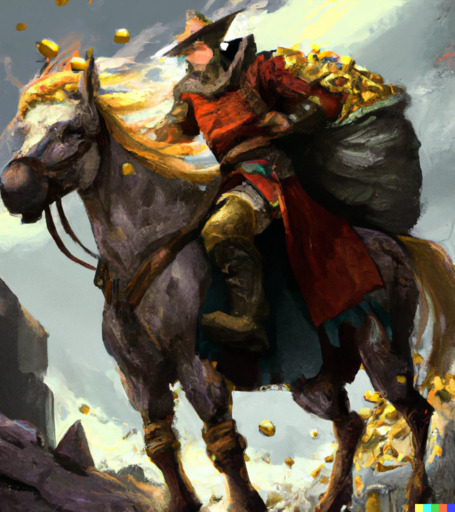
\includegraphics[width=\columnwidth]{equipment/tools goods and mounts}

        The world of Rise has a wide range of minor items like backpacks, blankets, and ten-foot poles.
        In general, the cost of those items is so insignificant from the perspective of an adventuring party that it's not worth the effort to track their cost in detail.
        A subset of particularly expensive items is included in \tref{Permanent Tools, Goods, and Mounts}.

        \subsection{Standard Adventuring Kit}\label{Standard Adventuring Kit}
          % Technically 15.2 gp and 50.5 pounds
          A standard adventuring kit is a rank 0 item (1 gp), weighs 50 pounds, and contains the following items:
          \begin{raggeditemize}
            \item Backpack
            \item Bedroll
            \item Flint and steel
            \item Rations, trail (8 days)
            \item Rope, hempen (60 ft.)
            \item Sack (empty)
            \item Tent
            \item Torch
            \item Waterskin
          \end{raggeditemize}
      \end{longtablepreface}

      \input{generated/permanent_tools_table.tex}
  \end{longcolumn}

  \input{generated/permanent_tools.tex}

  % Magic consumables are a loosely limited slot, but being consumable is a big downside.
  % They have the same power level as spells.
  \begin{longcolumn}
    \section{Consumables}\label{Consumables}

      \subsection{Potions}
        A potion is a magical liquid that is typically contained in a Fine vial.
        Drinking a potion, or administering a potion to an unconscious creature, requires a standard action.
        Potions cannot be safely mixed together without diluting their magic, so you cannot consume two potions with the same action.

        \input{generated/consumable_tools_table.tex}
  \end{longcolumn}

  \input{generated/consumable_tools.tex}

% Magic weapons are a highly limited slot.
% They have the same power level as self-attune spells.
\begin{longcolumn}
    \section{Magic Weapons}\label{Magic Weapons}
    \begin{longtablepreface}

      Magic weapons improve a character's combat abilities.
      They must be wielded to gain their effects.

      \parhead{Ranged Weapons and Ammunition} Any magical properties of a \weapontag{Projectile} weapon also apply to all ammunition fired from that weapon.

      \parhead{Craft Skills} The craft skills used to create and repair items are listed in parentheses before the item's description.
      All magic weapons simply use the same materials as the original, nonmagical weapon.

      \parhead{Property Limits} Normally, a weapon can only have one magic item property.
      \weapontag{Heavy} items can have two magic item properties instead of one.
    \end{longtablepreface}

    \input{generated/magic_weapons_table.tex}

\end{longcolumn}

\input{generated/magic_weapons.tex}

% Magic armor is a highly limited slot.
% They have the same power level as self-attune spells.
\begin{longcolumn}
  \section{Magic Armor}\label{Magic Armor}
    \begin{longtablepreface}
      Magic body armor must be worn to gain its effects, while magic shields must be wielded.
      You cannot imbue magic body armor effects on ordinary clothing, even if that clothing is worn on the body instead of armor.

      \parhead{Property Limits} A suit of body armor can only have one magic item property.
      A shield can also have one magic item property.
    \end{longtablepreface}

    \input{generated/magic_armor_table.tex}

\end{longcolumn}

\input{generated/magic_armor.tex}

% Magic apparel is a loosely limited slot.
% They are one rank behind self-attune spells.
\begin{longcolumn}
  \section{Magic Apparel}
    \begin{longtablepreface}
      
\includegraphics[width=\columnwidth]{equipment/magic apparel}
      Magic apparel items must be worn to gain their effects.

      \subsection{Body Slots}\label{Body Slots}
        The main limiting factor on how many items you can have equipped is your attunement points, not the physical location of your items on your body.
        However, there are limits to how many items you can wear of the same type, as described below.
        For item types not listed here, use reasonable judgment about what would be plausible.
        \begin{raggeditemize}
          \item Amulet: Up to 2
          \item Belt: Up to 2
          \item Boots: Up to 1
          \item Circlet: Up to 2
          \item Cloak: Up to 2
          \item Gauntlets: Up to 1 (separate from gloves)
          \item Gloves: Up to 1 (separate from gauntlets)
          \item Rings: Up to 5 per hand
          \item Tattoo: Any number, but only 1 per specific tattoo location
        \end{raggeditemize}

      \parhead{Property Limits} An apparel item can only have one magic item property.
    \end{longtablepreface}

    
\begin{longtablewrapper}
\begin{longtable}{p{15em} p{3em} p{6em} p{25em} p{3em}}

\lcaption{Apparel Items} \\
\tb{Name} & \tb{Level} & \tb{Typical Price} & \tb{Description} & \tb{Page} \tableheaderrule
Bracers of Archery & \nth{1} & 50 gp & Grants bow proficiency & \pageref{item:Bracers of Archery} \\
Belt of Healing & \nth{2} & 125 gp & Grants healing & \pageref{item:Belt of Healing} \\
Boots of the Winterlands & \nth{2} & 125 gp & Eases travel in cold areas & \pageref{item:Boots of the Winterlands} \\
Bracers of Armor & \nth{2} & 125 gp & Grants invisible armor & \pageref{item:Bracers of Armor} \\
Gauntlets of Improvisation & \nth{2} & 125 gp & Grants \plus1d damage with improvised weapons & \pageref{item:Gauntlets of Improvisation} \\
Ring of Elemental Endurance & \nth{2} & 125 gp & Grants tolerance of temperature extremes & \pageref{item:Ring of Elemental Endurance} \\
Shield of Bashing & \nth{2} & 125 gp & Grants \plus2 power & \pageref{item:Shield of Bashing} \\
Torchlight Gloves & \nth{2} & 125 gp & Sheds light as a torch & \pageref{item:Torchlight Gloves} \\
Ocular Circlet & \nth{3} & 250 gp & Can allow you to see at a distance & \pageref{item:Ocular Circlet} \\
Ring of Nourishment & \nth{3} & 250 gp & Provides food and water & \pageref{item:Ring of Nourishment} \\
Boots of Earth's Embrace & \nth{4} & 500 gp & Grants immunity to forced movement & \pageref{item:Boots of Earth's Embrace} \\
Boots of Elvenkind & \nth{4} & 500 gp & Grants \plus2 Stealth & \pageref{item:Boots of Elvenkind} \\
Circlet of Persuasion & \nth{4} & 500 gp & Grants \plus2 Persuasion & \pageref{item:Circlet of Persuasion} \\
Gauntlet of the Ram & \nth{4} & 500 gp & Knocks back foe when used to strike & \pageref{item:Gauntlet of the Ram} \\
Mask of Water Breathing & \nth{4} & 500 gp & Allows breathing water like air & \pageref{item:Mask of Water Breathing} \\
Throwing Gloves & \nth{4} & 500 gp & Allows throwing any item accurately & \pageref{item:Throwing Gloves} \\
Acid Coated & \nth{5} & 800 gp & Deals acid damage to anything it touches & \pageref{item:Acid Coated} \\
Amulet of Translocation & \nth{5} & 800 gp & Grants ability to teleport up to 30 feet & \pageref{item:Amulet of Translocation} \\
Circlet of Blasting & \nth{5} & 800 gp & Can blast foe with fire & \pageref{item:Circlet of Blasting} \\
Hidden Armor & \nth{5} & 800 gp & Can look like normal clothing & \pageref{item:Hidden Armor} \\
Protective Armor & \nth{5} & 800 gp & Grants \plus1 Armor defense & \pageref{item:Protective Armor} \\
Protective Shield & \nth{5} & 800 gp & Grants \plus1 Armor defense & \pageref{item:Protective Shield} \\
Shield of Arrow Catching & \nth{5} & 800 gp & Redirects small nearby projectiles to hit you & \pageref{item:Shield of Arrow Catching} \\
Shield of Arrow Deflection & \nth{5} & 800 gp & Blocks small projectiles & \pageref{item:Shield of Arrow Deflection} \\
Translocation & \nth{5} & 800 gp & Grants ability to teleport up to 30 feet & \pageref{item:Translocation} \\
Agile & \nth{6} & 1,200 gp & Grants \plus2 Reflex defense & \pageref{item:Agile} \\
Amulet of Health & \nth{6} & 1,200 gp & Grants 2 additional hit points & \pageref{item:Amulet of Health} \\
Amulet of Nondetection & \nth{6} & 1,200 gp & Grants \plus4 to defenses against detection & \pageref{item:Amulet of Nondetection} \\
Boots of Speed & \nth{6} & 1,200 gp & Increases speed by ten feet & \pageref{item:Boots of Speed} \\
Featherlight Armor & \nth{6} & 1,200 gp & Reduces encumbrance by 1 & \pageref{item:Featherlight Armor} \\
Fortified & \nth{6} & 1,200 gp & Grants \plus2 Fortitude defense & \pageref{item:Fortified} \\
Quilled Cloak & \nth{6} & 1,200 gp & Deals damage to creatures that grapple you & \pageref{item:Quilled Cloak} \\
Willguard & \nth{6} & 1,200 gp & Grants \plus2 Mental defense & \pageref{item:Willguard} \\
Anchoring & \nth{7} & 1,800 gp & Protects you from most forced movement attacks & \pageref{item:Anchoring} \\
Armor of Fortification & \nth{7} & 1,800 gp & Reduces critical hits from strikes & \pageref{item:Armor of Fortification} \\
Boots of Water Walking & \nth{7} & 1,800 gp & Allows walking on liquids & \pageref{item:Boots of Water Walking} \\
Boots of the Skydancer & \nth{7} & 1,800 gp & Can walk on air & \pageref{item:Boots of the Skydancer} \\
Bracers of Archery, Greater & \nth{7} & 1,800 gp & Grants bow proficiency, \plus1 ranged accuracy & \pageref{item:Bracers of Archery, Greater} \\
Bracers of Repulsion & \nth{7} & 1,800 gp & Can knock nearby creatures back & \pageref{item:Bracers of Repulsion} \\
Crown of Lightning & \nth{7} & 1,800 gp & Continuously damages nearby enemies & \pageref{item:Crown of Lightning} \\
Gauntlet of the Ram, Greater & \nth{7} & 1,800 gp & Knocks back foe farther when use to strike & \pageref{item:Gauntlet of the Ram, Greater} \\
Gauntlets of Improvisation, Greater & \nth{7} & 1,800 gp & Grants \plus2d damage with improvised weapons & \pageref{item:Gauntlets of Improvisation, Greater} \\
Gloves of Spell Investment & \nth{7} & 1,800 gp & Can invest a spell to cast later & \pageref{item:Gloves of Spell Investment} \\
Hexward Amulet & \nth{7} & 1,800 gp & Grants \plus1 defenses against targeted magical attacks & \pageref{item:Hexward Amulet} \\
Lifekeeping Belt & \nth{7} & 1,800 gp & Grants \plus1 bonus to \glossterm{vital rolls} & \pageref{item:Lifekeeping Belt} \\
Ring of Sustenance & \nth{7} & 1,800 gp & Provides food, water, and rest & \pageref{item:Ring of Sustenance} \\
Amulet of Mighty Fists & \nth{8} & 2,750 gp & Grants \plus2 power with natural and unarmed attacks & \pageref{item:Amulet of Mighty Fists} \\
Armor of Energy Resistance & \nth{8} & 2,750 gp & Reduces energy damage & \pageref{item:Armor of Energy Resistance} \\
Armor of Invulnerability & \nth{8} & 2,750 gp & Reduces physical damage & \pageref{item:Armor of Invulnerability} \\
Assassin's Cloak & \nth{8} & 2,750 gp & Grants invisibility while inactive & \pageref{item:Assassin's Cloak} \\
Avian Cloak & \nth{8} & 2,750 gp & Grants a glide speed & \pageref{item:Avian Cloak} \\
Belt of Healing, Greater & \nth{8} & 2,750 gp & Grants more healing & \pageref{item:Belt of Healing, Greater} \\
Boots of Gravitation & \nth{8} & 2,750 gp & Redirects personal gravity & \pageref{item:Boots of Gravitation} \\
Cloak of Mist & \nth{8} & 2,750 gp & Fills nearby area with fog & \pageref{item:Cloak of Mist} \\
Ring of Protection & \nth{8} & 2,750 gp & Grants \plus1 to Armor and Reflex defenses & \pageref{item:Ring of Protection} \\
Shield of Boulder Catching & \nth{8} & 2,750 gp & Redirects large nearby projectiles to hit you & \pageref{item:Shield of Boulder Catching} \\
Shield of Boulder Deflection & \nth{8} & 2,750 gp & Can block large projectiles & \pageref{item:Shield of Boulder Deflection} \\
Crown of Flame & \nth{9} & 4,000 gp & Grants nearby allies immunity to fire damage & \pageref{item:Crown of Flame} \\
Greatreach Bracers & \nth{9} & 4,000 gp & Increases reach by five feet & \pageref{item:Greatreach Bracers} \\
Hidden Armor, Greater & \nth{9} & 4,000 gp & Can look and sound like normal clothing & \pageref{item:Hidden Armor, Greater} \\
Mask of Air & \nth{9} & 4,000 gp & Allows breathing in any environment & \pageref{item:Mask of Air} \\
Ocular Circlet, Greater & \nth{9} & 4,000 gp & Can allow you to see at a greater distance & \pageref{item:Ocular Circlet, Greater} \\
Ring of Angel's Grace & \nth{9} & 4,000 gp & Grants \plus2 Mental and slows falls & \pageref{item:Ring of Angel's Grace} \\
Boots of Speed, Greater & \nth{10} & 6,500 gp & Increases speed by twenty feet & \pageref{item:Boots of Speed, Greater} \\
Circlet of Blasting, Greater & \nth{10} & 6,500 gp & Can blast foe with intense fire & \pageref{item:Circlet of Blasting, Greater} \\
Crater Boots & \nth{10} & 6,500 gp & Deals your falling damage to enemies & \pageref{item:Crater Boots} \\
Titan Gauntlets & \nth{10} & 6,500 gp & Grants \plus2 \glossterm{mundane} power & \pageref{item:Titan Gauntlets} \\
Winged Boots & \nth{10} & 6,500 gp & Grants limited flight & \pageref{item:Winged Boots} \\
Amulet of Translocation, Greater & \nth{11} & 10,000 gp & Grants ability to teleport up to 100 feet & \pageref{item:Amulet of Translocation, Greater} \\
Crown of Thunder & \nth{11} & 10,000 gp & Continously deafens nearby enemies & \pageref{item:Crown of Thunder} \\
Shield of Arrow Catching, Greater & \nth{11} & 10,000 gp & Selectively redirects small nearby projectiles to hit you & \pageref{item:Shield of Arrow Catching, Greater} \\
Shield of Bashing, Greater & \nth{11} & 10,000 gp & Grants \plus4 power & \pageref{item:Shield of Bashing, Greater} \\
Translocation, Greater & \nth{11} & 10,000 gp & Grants ability to teleport up to 100 feet & \pageref{item:Translocation, Greater} \\
Amulet of the Planes & \nth{12} & 16,000 gp & Aids travel with \ritual{plane shift} & \pageref{item:Amulet of the Planes} \\
Armor of Fortification, Mystic & \nth{12} & 16,000 gp & Reduces critical hits from all attacks & \pageref{item:Armor of Fortification, Mystic} \\
Boots of Freedom & \nth{12} & 16,000 gp & Grants immunity to almost all mobility restrictions & \pageref{item:Boots of Freedom} \\
Featherlight Armor, Greater & \nth{12} & 16,000 gp & Reduces encumbrance by 2 & \pageref{item:Featherlight Armor, Greater} \\
Greater Quilled Cloak & \nth{12} & 16,000 gp & Deals more damage to creatures that grapple you & \pageref{item:Greater Quilled Cloak} \\
Ring of Energy Resistance & \nth{12} & 16,000 gp & Reduces energy damage & \pageref{item:Ring of Energy Resistance} \\
Seven League Boots & \nth{12} & 16,000 gp & Teleport seven leages with a step & \pageref{item:Seven League Boots} \\
Shield of Mystic Reflection & \nth{12} & 16,000 gp & React to reflect magical attacks & \pageref{item:Shield of Mystic Reflection} \\
Anchoring, Greater & \nth{13} & 25,000 gp & Protects you from all forced movement and teleportation attacks & \pageref{item:Anchoring, Greater} \\
Assassin's Cloak, Greater & \nth{13} & 25,000 gp & Grants longer invisibility while inactive & \pageref{item:Assassin's Cloak, Greater} \\
Boots of the Skydancer, Greater & \nth{13} & 25,000 gp & description & \pageref{item:Boots of the Skydancer, Greater} \\
Crown of Frost & \nth{13} & 25,000 gp & Continuously damages nearby enemies & \pageref{item:Crown of Frost} \\
Gloves of Spell Investment, Greater & \nth{13} & 25,000 gp & Can invest two spells to cast later & \pageref{item:Gloves of Spell Investment, Greater} \\
Hexproof Amulet, Greater & \nth{13} & 25,000 gp & Grants \plus2 defenses against targeted magical attacks & \pageref{item:Hexproof Amulet, Greater} \\
Lifekeeping Belt, Greater & \nth{13} & 25,000 gp & Grants \plus2 bonus to \glossterm{vital rolls} & \pageref{item:Lifekeeping Belt, Greater} \\
Vanishing Cloak & \nth{13} & 25,000 gp & Can teleport a short distance and grant invisibility & \pageref{item:Vanishing Cloak} \\
Amulet of Nondetection, Greater & \nth{14} & 37,000 gp & Grants \plus8 to defenses against detection & \pageref{item:Amulet of Nondetection, Greater} \\
Armor of Energy Resistance, Greater & \nth{14} & 37,000 gp & Significantly reduces energy damage & \pageref{item:Armor of Energy Resistance, Greater} \\
Armor of Invulnerability & \nth{14} & 37,000 gp & Significantly reduces physical damage & \pageref{item:Armor of Invulnerability} \\
Belt of Healing, Supreme & \nth{14} & 37,000 gp & Grants more healing & \pageref{item:Belt of Healing, Supreme} \\
Boots of Speed, Supreme & \nth{14} & 37,000 gp & Increases speed by thirty feet & \pageref{item:Boots of Speed, Supreme} \\
Protective Armor, Greater & \nth{14} & 37,000 gp & Grants \plus2 Armor defense & \pageref{item:Protective Armor, Greater} \\
Protective Shield, Greater & \nth{14} & 37,000 gp & Grants \plus2 Armor defense & \pageref{item:Protective Shield, Greater} \\
Shield of Arrow Deflection, Greater & \nth{14} & 37,000 gp & Blocks small projectiles & \pageref{item:Shield of Arrow Deflection, Greater} \\
Agile, Greater & \nth{15} & 55,000 gp & Grants \plus4 Reflex defense & \pageref{item:Agile, Greater} \\
Amulet of Health, Greater & \nth{15} & 55,000 gp & Grants 4 additional hit points & \pageref{item:Amulet of Health, Greater} \\
Armor of Fortification, Greater & \nth{15} & 55,000 gp & Drastically reduces critical hits from strikes & \pageref{item:Armor of Fortification, Greater} \\
Bracers of Repulsion, Greater & \nth{15} & 55,000 gp & Can knock many nearby creatures back & \pageref{item:Bracers of Repulsion, Greater} \\
Fortified, Greater & \nth{15} & 55,000 gp & Grants \plus4 Fortitude defense & \pageref{item:Fortified, Greater} \\
Ring of Regeneration & \nth{15} & 55,000 gp & Automatically removes vital wounds & \pageref{item:Ring of Regeneration} \\
Willguard, Greater & \nth{15} & 55,000 gp & Grants \plus4 Mental defense & \pageref{item:Willguard, Greater} \\
Amulet of Mighty Fists, Greater & \nth{16} & 85,000 gp & Grants \plus4 power with natural and unarmed attacks & \pageref{item:Amulet of Mighty Fists, Greater} \\
Astral Boots & \nth{16} & 85,000 gp & Allows teleporting instead of moving & \pageref{item:Astral Boots} \\
Circlet of Blasting, Supreme & \nth{16} & 85,000 gp & Can blast foe with supremely intense fire & \pageref{item:Circlet of Blasting, Supreme} \\
Cloak of Mist, Greater & \nth{16} & 85,000 gp & Fills nearby area with thick fog & \pageref{item:Cloak of Mist, Greater} \\
Ring of Protection, Greater & \nth{16} & 85,000 gp & Grants \plus2 to Armor and Reflex defenses & \pageref{item:Ring of Protection, Greater} \\
Amulet of Translocation, Supreme & \nth{17} & 125,000 gp & Grants ability to teleport up to 300 feet & \pageref{item:Amulet of Translocation, Supreme} \\
Greatreach Bracers, Greater & \nth{17} & 125,000 gp & Increases reach by ten feet & \pageref{item:Greatreach Bracers, Greater} \\
Shield of Boulder Deflection, Greater & \nth{17} & 125,000 gp & Blocks large projectiles & \pageref{item:Shield of Boulder Deflection, Greater} \\
Translocation, Supreme & \nth{17} & 125,000 gp & Grants ability to teleport up to 300 feet & \pageref{item:Translocation, Supreme} \\
Featherlight Armor, Supreme & \nth{18} & 190,000 gp & Reduces encumbrance by 2 & \pageref{item:Featherlight Armor, Supreme} \\
Supreme Quilled Cloak & \nth{18} & 190,000 gp & Deals even more damage to creatures that grapple you & \pageref{item:Supreme Quilled Cloak} \\
Hexproof Amulet, Supreme & \nth{19} & 280,000 gp & Grants \plus3 defenses against targeted magical attacks & \pageref{item:Hexproof Amulet, Supreme} \\
Lifekeeping Belt, Supreme & \nth{19} & 280,000 gp & Grants \plus3 bonus to \glossterm{vital rolls} & \pageref{item:Lifekeeping Belt, Supreme} \\
Titan Gauntlets, Greater & \nth{19} & 280,000 gp & Grants \plus4 \glossterm{mundane} power & \pageref{item:Titan Gauntlets, Greater} \\
Armor of Energy Resistance, Supreme & \nth{20} & 400,000 gp & Drastically reduces energy damage & \pageref{item:Armor of Energy Resistance, Supreme} \\
Armor of Invulnerability, Greater & \nth{20} & 400,000 gp & Drastically reduces physical damage & \pageref{item:Armor of Invulnerability, Greater} \\
Shield of Bashing, Supreme & \nth{20} & 400,000 gp & Grants \plus6 power & \pageref{item:Shield of Bashing, Supreme} \\

\end{longtable}
\end{longtablewrapper}


\end{longcolumn}

\lowercase{\hypertarget{item:Amulet of Mighty Fists}{}}\label{item:Amulet of Mighty Fists}
\hypertarget{item:Amulet of Mighty Fists}{\subsubsection{Amulet of Mighty Fists\hfill\nth{6}}}
You gain a \plus1d bonus to \glossterm{strike damage} with \glossterm{unarmed attacks} and natural weapons.
\parhead*{Tags} \glossterm{Enhancement}
\parhead*{Materials} Jewelry
\lowercase{\hypertarget{item:Amulet of Mighty Fists, Greater}{}}\label{item:Amulet of Mighty Fists, Greater}
\hypertarget{item:Amulet of Mighty Fists, Greater}{\subsubsection{Amulet of Mighty Fists, Greater\hfill\nth{14}}}
You gain a \plus2d bonus to \glossterm{strike damage} with \glossterm{unarmed attacks} and natural weapons.
\parhead*{Tags} \glossterm{Enhancement}
\parhead*{Materials} Jewelry
\lowercase{\hypertarget{item:Armor of Energy Resistance}{}}\label{item:Armor of Energy Resistance}
\hypertarget{item:Armor of Energy Resistance}{\subsubsection{Armor of Energy Resistance\hfill\nth{4}}}
You have \glossterm{damage reduction} equal to the item's \glossterm{power} against \glossterm{energy damage}.
Whenever you resist energy with this item, it sheds light as a torch until the end of the next round.
The color of the light depends on the energy damage resisted: blue for cold, yellow for electricity, red for fire, and brown for sonic.
\parhead*{Tags} \glossterm{Shielding}
\parhead*{Materials} Bone, metal
\lowercase{\hypertarget{item:Armor of Energy Resistance, Greater}{}}\label{item:Armor of Energy Resistance, Greater}
\hypertarget{item:Armor of Energy Resistance, Greater}{\subsubsection{Armor of Energy Resistance, Greater\hfill\nth{12}}}
This item functions like the \mitem{armor of energy resistance} item, except that the damage reduction is equal to twice the item's \glossterm{power}.
\parhead*{Tags} \glossterm{Shielding}
\parhead*{Materials} Bone, metal
\lowercase{\hypertarget{item:Armor of Fortification}{}}\label{item:Armor of Fortification}
\hypertarget{item:Armor of Fortification}{\subsubsection{Armor of Fortification\hfill\nth{7}}}
You gain a \plus5 bonus to defenses when determining whether a \glossterm{strike} gets a \glossterm{critical hit} against you instead of a normal hit.
\parhead*{Tags} \glossterm{Imbuement}
\parhead*{Materials} Bone, metal
\lowercase{\hypertarget{item:Armor of Fortification, Greater}{}}\label{item:Armor of Fortification, Greater}
\hypertarget{item:Armor of Fortification, Greater}{\subsubsection{Armor of Fortification, Greater\hfill\nth{15}}}
This item functions like the \mitem{armor of fortification} item, except that the bonus increases to \plus10.
\parhead*{Tags} \glossterm{Imbuement}
\parhead*{Materials} Bone, metal
\lowercase{\hypertarget{item:Armor of Fortification, Mystic}{}}\label{item:Armor of Fortification, Mystic}
\hypertarget{item:Armor of Fortification, Mystic}{\subsubsection{Armor of Fortification, Mystic\hfill\nth{12}}}
This item functions like the \mitem{armor of fortification} item, except that it applies against all attacks instead of only against; \glossterm{strikes}.
\parhead*{Tags} \glossterm{Imbuement}
\parhead*{Materials} Bone, metal
\lowercase{\hypertarget{item:Armor of Invulnerability}{}}\label{item:Armor of Invulnerability}
\hypertarget{item:Armor of Invulnerability}{\subsubsection{Armor of Invulnerability\hfill\nth{8}}}
You have \glossterm{damage reduction} equal to this item's \glossterm{power} against damage from \glossterm{physical attacks}.
\parhead*{Tags} \glossterm{Shielding}
\parhead*{Materials} Bone, metal
\lowercase{\hypertarget{item:Armor of Invulnerability, Greater}{}}\label{item:Armor of Invulnerability, Greater}
\hypertarget{item:Armor of Invulnerability, Greater}{\subsubsection{Armor of Invulnerability, Greater\hfill\nth{16}}}
This item functions like the \mitem{armor of invulnerability} item, except that the damage reduction is equal to twice the item's \glossterm{power}.
You have \glossterm{damage reduction} equal to the item's \glossterm{power} against damage from \glossterm{physical attacks}.
\parhead*{Tags} \glossterm{Shielding}
\parhead*{Materials} Bone, metal
\lowercase{\hypertarget{item:Armor of Magic Resistance}{}}\label{item:Armor of Magic Resistance}
\hypertarget{item:Armor of Magic Resistance}{\subsubsection{Armor of Magic Resistance\hfill\nth{14}}}
You have \glossterm{magic resistance} equal to 5 + the item's \glossterm{power}.
\parhead*{Tags} \glossterm{Shielding}
\parhead*{Materials} Bone, metal
\lowercase{\hypertarget{item:Assassin's Cloak}{}}\label{item:Assassin's Cloak}
\hypertarget{item:Assassin's Cloak}{\subsubsection{Assassin's Cloak\hfill\nth{7}}}
At the end of each round, if you took no actions that round, you become \glossterm{invisible} until the end of the next round.
\parhead*{Tags} \glossterm{Glamer}
\parhead*{Materials} Textiles
\lowercase{\hypertarget{item:Assassin's Cloak, Greater}{}}\label{item:Assassin's Cloak, Greater}
\hypertarget{item:Assassin's Cloak, Greater}{\subsubsection{Assassin's Cloak, Greater\hfill\nth{17}}}
At the end of each round, if you did not attack a creature that round, you become \glossterm{invisible} until the end of the next round.
\parhead*{Tags} \glossterm{Glamer}
\parhead*{Materials} Textiles
\lowercase{\hypertarget{item:Astral Boots}{}}\label{item:Astral Boots}
\hypertarget{item:Astral Boots}{\subsubsection{Astral Boots\hfill\nth{16}}}
Whenever you move, you can teleport the same distance instead.
This does not change the total distance you can move, but you can teleport in any direction, even vertically.
You cannot teleport to locations you do not have \glossterm{line of sight} and \glossterm{line of effect} to.
\parhead*{Tags} \glossterm{Teleportation}
\parhead*{Materials} Bone, leather, metal
\lowercase{\hypertarget{item:Belt of Healing}{}}\label{item:Belt of Healing}
\hypertarget{item:Belt of Healing}{\subsubsection{Belt of Healing\hfill\nth{1}}}
When you use the \textit{recover} action, you heal \plus1d hit points.
\parhead*{Tags} \glossterm{Life}
\parhead*{Materials} Leather, textiles
\lowercase{\hypertarget{item:Belt of Healing, Greater}{}}\label{item:Belt of Healing, Greater}
\hypertarget{item:Belt of Healing, Greater}{\subsubsection{Belt of Healing, Greater\hfill\nth{8}}}
When you use the \textit{recover} action, you heal \plus2d hit points.
\parhead*{Tags} \glossterm{Life}
\parhead*{Materials} Leather, textiles
\lowercase{\hypertarget{item:Belt of Heroic Recovery}{}}\label{item:Belt of Heroic Recovery}
\hypertarget{item:Belt of Heroic Recovery}{\subsubsection{Belt of Heroic Recovery\hfill\nth{6}}}
% TODO: timing?
As an \glossterm{immediate action} when you get a \glossterm{critical hit}, you can take the \textit{recover} action.
\parhead*{Tags} \glossterm{Life}
\parhead*{Materials} Leather, textiles
\lowercase{\hypertarget{item:Boots of Earth's Embrace}{}}\label{item:Boots of Earth's Embrace}
\hypertarget{item:Boots of Earth's Embrace}{\subsubsection{Boots of Earth's Embrace\hfill\nth{4}}}
While you are standing on solid ground, you are immune to effects that would force you to move.
This does not protect you from other effects of those attacks, such as damage.
\parhead*{Tags} \glossterm{Earth}, \glossterm{Enhancement}
\parhead*{Materials} Bone, leather, metal
\lowercase{\hypertarget{item:Boots of Freedom}{}}\label{item:Boots of Freedom}
\hypertarget{item:Boots of Freedom}{\subsubsection{Boots of Freedom\hfill\nth{6}}}
You are immune to effects that restrict your mobility.
This removes all penalties you would suffer for acting underwater, except for those relating to using ranged weapons.
This does not prevent you from being \grappled, but you gain a \plus10 bonus to your defense against \glossterm{grapple} attacks.
\parhead*{Tags} \glossterm{Imbuement}
\parhead*{Materials} Bone, leather, metal
\lowercase{\hypertarget{item:Boots of Freedom, Greater}{}}\label{item:Boots of Freedom, Greater}
\hypertarget{item:Boots of Freedom, Greater}{\subsubsection{Boots of Freedom, Greater\hfill\nth{12}}}
These boots function like \mitem{boots of freedom}, except that you are also immune to being \grappled.
\parhead*{Tags} \glossterm{Imbuement}
\parhead*{Materials} Bone, leather, metal
\lowercase{\hypertarget{item:Boots of Gravitation}{}}\label{item:Boots of Gravitation}
\hypertarget{item:Boots of Gravitation}{\subsubsection{Boots of Gravitation\hfill\nth{8}}}
While these boots are within 5 feet of a solid surface, gravity pulls you towards the solid surface closest to your boots rather than in the normal direction.
This can allow you to walk easily on walls or even ceilings.
\parhead*{Tags} \glossterm{Imbuement}
\parhead*{Materials} Bone, leather, metal
\lowercase{\hypertarget{item:Boots of Speed}{}}\label{item:Boots of Speed}
\hypertarget{item:Boots of Speed}{\subsubsection{Boots of Speed\hfill\nth{5}}}
You gain a \plus10 foot bonus to your speed in all your movement modes, up to a maximum of double your normal speed.
\parhead*{Tags} \glossterm{Temporal}
\parhead*{Materials} Bone, leather, metal
\lowercase{\hypertarget{item:Boots of Speed, Greater}{}}\label{item:Boots of Speed, Greater}
\hypertarget{item:Boots of Speed, Greater}{\subsubsection{Boots of Speed, Greater\hfill\nth{13}}}
You gain a \plus30 foot bonus to your speed in all your movement modes, up to a maximum of double your normal speed.
\parhead*{Tags} \glossterm{Temporal}
\parhead*{Materials} Bone, leather, metal
\lowercase{\hypertarget{item:Boots of Water Walking}{}}\label{item:Boots of Water Walking}
\hypertarget{item:Boots of Water Walking}{\subsubsection{Boots of Water Walking\hfill\nth{7}}}
You treat the surface of all liquids as if they were firm ground.
Your feet hover about an inch above the liquid's surface, allowing you to traverse dangerous liquids without harm as long as the surface is calm.
If you are below the surface of the liquid, you rise towards the surface at a rate of 60 feet per round.
Thick liquids, such as mud and lava, may cause you to rise more slowly.
\parhead*{Tags} \glossterm{Imbuement}
\parhead*{Materials} Bone, leather, metal
\lowercase{\hypertarget{item:Boots of the Winterlands}{}}\label{item:Boots of the Winterlands}
\hypertarget{item:Boots of the Winterlands}{\subsubsection{Boots of the Winterlands\hfill\nth{2}}}
You can travel across snow and ice without slipping or suffering movement penalties for the terrain.
% TODO: degree symbol?
In addition, the boots keep you warn, protecting you in environments as cold as \minus50 Fahrenheit.
\parhead*{Tags} \glossterm{Enhancement}
\parhead*{Materials} Bone, leather, metal
\lowercase{\hypertarget{item:Bracers of Archery}{}}\label{item:Bracers of Archery}
\hypertarget{item:Bracers of Archery}{\subsubsection{Bracers of Archery\hfill\nth{1}}}
You are proficient with bows.
\parhead*{Tags} \glossterm{Enhancement}
\parhead*{Materials} Bone, leather, metal, wood
\lowercase{\hypertarget{item:Bracers of Armor}{}}\label{item:Bracers of Armor}
\hypertarget{item:Bracers of Armor}{\subsubsection{Bracers of Armor\hfill\nth{2}}}
You gain a \plus2 bonus to Armor defense.
The protection from these bracers is treated as body armor, and it does not stack with any other body armor you wear.
\parhead*{Tags} \glossterm{Shielding}
\parhead*{Materials} Bone, leather, metal, wood
\lowercase{\hypertarget{item:Bracers of Repulsion}{}}\label{item:Bracers of Repulsion}
\hypertarget{item:Bracers of Repulsion}{\subsubsection{Bracers of Repulsion\hfill\nth{4}}}
Whenever a creature hits you with a melee \glossterm{strike} during the \glossterm{action phase},
you can spend an \glossterm{action point} to use this item as an \glossterm{immediate action}.
If you do, you make a \glossterm{shove} attack against that creature during the \glossterm{delayed action phase}, using this item's power in place of your Strength.
\parhead*{Tags} \glossterm{Telekinesis}
\parhead*{Materials} Bone, leather, metal, wood
\lowercase{\hypertarget{item:Bracers of Repulsion, Greater}{}}\label{item:Bracers of Repulsion, Greater}
\hypertarget{item:Bracers of Repulsion, Greater}{\subsubsection{Bracers of Repulsion, Greater\hfill\nth{11}}}
This item functions like the \mitem{bracers of repulsion} item, except that it does not cost an action point to use.
\parhead*{Tags} \glossterm{Telekinesis}
\parhead*{Materials} Bone, leather, metal, wood
\lowercase{\hypertarget{item:Cloak of Mist}{}}\label{item:Cloak of Mist}
\hypertarget{item:Cloak of Mist}{\subsubsection{Cloak of Mist\hfill\nth{8}}}
Fog constantly fills an \areamed radius emanation from you.
This fog does not fully block sight, but it provides \concealment.
If a 5-foot square of fog takes fire damage equal to half this item's \glossterm{power}, the fog disappears from that area until the end of the next round.
\parhead*{Tags} \glossterm{Fog}, \glossterm{Manifestation}
\parhead*{Materials} Textiles
\lowercase{\hypertarget{item:Cloak of Mist, Greater}{}}\label{item:Cloak of Mist, Greater}
\hypertarget{item:Cloak of Mist, Greater}{\subsubsection{Cloak of Mist, Greater\hfill\nth{16}}}
A thick fog constantly fills an \areamed radius emanation from you.
This fog completely blocks sight beyond 10 feet.
Within that range, it still provides \concealment.
If a 5-foot square of fog takes fire damage equal to this item's \glossterm{power}, the fog disappears from that area until the end of the next round.
\parhead*{Tags} \glossterm{Fog}, \glossterm{Manifestation}
\parhead*{Materials} Textiles
\lowercase{\hypertarget{item:Crown of Flame}{}}\label{item:Crown of Flame}
\hypertarget{item:Crown of Flame}{\subsubsection{Crown of Flame\hfill\nth{5}}}
This crown is continuously on fire.
The flame sheds light as a torch.
You and all allies within an \arealarge radius emanation from you are immune to fire damage.
\parhead*{Tags} \glossterm{Fire}
\parhead*{Materials} Bone, metal
\lowercase{\hypertarget{item:Crown of Frost}{}}\label{item:Crown of Frost}
\hypertarget{item:Crown of Frost}{\subsubsection{Crown of Frost\hfill\nth{11}}}
At the end of each \glossterm{action phase}, you make a Power vs. Fortitude attack against all enemies within an \areamed radius emanation from you.
A hit deals cold \glossterm{standard damage} \minus3d.
Each creature that takes damage in this way is \fatigued until the end of the next round.
\parhead*{Tags} \glossterm{Cold}
\parhead*{Materials} Bone, metal
\lowercase{\hypertarget{item:Crown of Lightning}{}}\label{item:Crown of Lightning}
\hypertarget{item:Crown of Lightning}{\subsubsection{Crown of Lightning\hfill\nth{7}}}
This crown continuously crackles with electricity.
The constant sparks shed light as a torch.
At the end of each \glossterm{action phase}, you make a Power vs. Reflex attack against all enemies within an \areamed radius emanation from you.
A hit deals electricity \glossterm{standard damage} \minus3d.
\parhead*{Tags} \glossterm{Electricity}
\parhead*{Materials} Bone, metal
\lowercase{\hypertarget{item:Crown of Thunder}{}}\label{item:Crown of Thunder}
\hypertarget{item:Crown of Thunder}{\subsubsection{Crown of Thunder\hfill\nth{9}}}
The crown constantly emits a low-pitched rumbling.
To you and your allies, the sound is barely perceptible.
However, all enemies within an \arealarge radius emanation from you hear the sound as a deafening, continuous roll of thunder.
The noise blocks out all other sounds quieter than thunder, causing them to be \deafened while they remain in the area and until the end of the next round after they leave.
\parhead*{Tags} \glossterm{Sonic}
\parhead*{Materials} Bone, metal
\lowercase{\hypertarget{item:Featherlight Armor}{}}\label{item:Featherlight Armor}
\hypertarget{item:Featherlight Armor}{\subsubsection{Featherlight Armor\hfill\nth{4}}}
This armor's \glossterm{encumbrance penalty} is reduced by 2.
\parhead*{Tags} \glossterm{Enhancement}
\parhead*{Materials} Bone, metal
\lowercase{\hypertarget{item:Featherlight Armor, Greater}{}}\label{item:Featherlight Armor, Greater}
\hypertarget{item:Featherlight Armor, Greater}{\subsubsection{Featherlight Armor, Greater\hfill\nth{10}}}
This armor's \glossterm{encumbrance penalty} is reduced by 4.
\parhead*{Tags} \glossterm{Enhancement}
\parhead*{Materials} Bone, metal
\lowercase{\hypertarget{item:Gauntlet of the Ram}{}}\label{item:Gauntlet of the Ram}
\hypertarget{item:Gauntlet of the Ram}{\subsubsection{Gauntlet of the Ram\hfill\nth{2}}}
If you hit on a \glossterm{strike} with this gauntlet during the \glossterm{action phse}, you can attempt to \glossterm{shove} your foe during the \glossterm{delayed action phase}.
Making a strike with this gauntlet is equivalent to an \glossterm{unarmed attack}.
You do not need to move with your foe to push it back the full distance.
\parhead*{Tags} \glossterm{Telekinesis}
\parhead*{Materials} Bone, metal, wood
\lowercase{\hypertarget{item:Gauntlet of the Ram, Greater}{}}\label{item:Gauntlet of the Ram, Greater}
\hypertarget{item:Gauntlet of the Ram, Greater}{\subsubsection{Gauntlet of the Ram, Greater\hfill\nth{7}}}
This item functions like the \mitem{gauntlet of the ram}, except that you gain a bonus to the \glossterm{shove} attack equal to the damage you dealt with the \glossterm{strike}.
\parhead*{Tags} \glossterm{Telekinesis}
\parhead*{Materials} Bone, metal, wood
\lowercase{\hypertarget{item:Gauntlets of Improvisation}{}}\label{item:Gauntlets of Improvisation}
\hypertarget{item:Gauntlets of Improvisation}{\subsubsection{Gauntlets of Improvisation\hfill\nth{2}}}
You gain a \plus1d bonus to damage with \glossterm{improvised weapons}.
\parhead*{Tags} \glossterm{Enhancement}
\parhead*{Materials} Bone, metal, wood
\lowercase{\hypertarget{item:Gauntlets of Improvisation, Greater}{}}\label{item:Gauntlets of Improvisation, Greater}
\hypertarget{item:Gauntlets of Improvisation, Greater}{\subsubsection{Gauntlets of Improvisation, Greater\hfill\nth{7}}}
This item functions like the \mitem{gauntlets of improvisation}, except that the damage bonus is increased to \plus2d.
\parhead*{Tags} \glossterm{Enhancement}
\parhead*{Materials} Bone, metal, wood
\lowercase{\hypertarget{item:Greatreach Bracers}{}}\label{item:Greatreach Bracers}
\hypertarget{item:Greatreach Bracers}{\subsubsection{Greatreach Bracers\hfill\nth{9}}}
Your \glossterm{reach} is increased by 5 feet.
\parhead*{Tags} \glossterm{Imbuement}
\parhead*{Materials} Bone, leather, metal, wood
\lowercase{\hypertarget{item:Greatreach Bracers, Greater}{}}\label{item:Greatreach Bracers, Greater}
\hypertarget{item:Greatreach Bracers, Greater}{\subsubsection{Greatreach Bracers, Greater\hfill\nth{17}}}
Your \glossterm{reach} is increased by 10 feet.
\parhead*{Tags} \glossterm{Imbuement}
\parhead*{Materials} Bone, leather, metal, wood
\lowercase{\hypertarget{item:Hexproof Cloak}{}}\label{item:Hexproof Cloak}
\hypertarget{item:Hexproof Cloak}{\subsubsection{Hexproof Cloak\hfill\nth{18}}}
All \glossterm{magical} abilities that target you directly fail to affect you.
This does not protect you from abilities that affect an area.
\parhead*{Tags} \glossterm{Thaumaturgy}
\parhead*{Materials} Textiles
\lowercase{\hypertarget{item:Hexward Cloak}{}}\label{item:Hexward Cloak}
\hypertarget{item:Hexward Cloak}{\subsubsection{Hexward Cloak\hfill\nth{10}}}
You gain a \plus5 bonus to defenses against \glossterm{magical} abilities that target you directly.
This does not protect you from abilities that affect an area.
\parhead*{Tags} \glossterm{Thaumaturgy}
\parhead*{Materials} Textiles
\lowercase{\hypertarget{item:Hidden Armor}{}}\label{item:Hidden Armor}
\hypertarget{item:Hidden Armor}{\subsubsection{Hidden Armor\hfill\nth{4}}}
As a standard action, you can use this item.
If you do, it appears to change shape and form to assume the shape of a normal set of clothing.
You may choose the design of the clothing.
The item retains all of its properties, including weight and sound, while disguised in this way.
Only its visual appearance is altered.
Alternately, you may return the armor to its original appearance.
\parhead*{Tags} \glossterm{Glamer}
\parhead*{Materials} Bone, metal
\lowercase{\hypertarget{item:Hidden Armor, Greater}{}}\label{item:Hidden Armor, Greater}
\hypertarget{item:Hidden Armor, Greater}{\subsubsection{Hidden Armor, Greater\hfill\nth{9}}}
This item functions like the \mitem{hidden armor} item, except that the item also makes sound appropriate to its disguised form while disguised.
\parhead*{Tags} \glossterm{Alteration}
\parhead*{Materials} Bone, metal
\lowercase{\hypertarget{item:Mask of Air}{}}\label{item:Mask of Air}
\hypertarget{item:Mask of Air}{\subsubsection{Mask of Air\hfill\nth{9}}}
If you breathe through this mask, you breathe in clean, fresh air, regardless of your environment.
This can protect you from inhaled poisons and similar effects.
\parhead*{Tags} \glossterm{Imbuement}
\parhead*{Materials} Textiles
\lowercase{\hypertarget{item:Mask of Water Breathing}{}}\label{item:Mask of Water Breathing}
\hypertarget{item:Mask of Water Breathing}{\subsubsection{Mask of Water Breathing\hfill\nth{4}}}
You can breathe water through this mask as easily as a human breaths air.
This does not grant you the ability to breathe other liquids.
\parhead*{Tags} \glossterm{Imbuement}
\parhead*{Materials} Textiles
\lowercase{\hypertarget{item:Ring of Elemental Endurance}{}}\label{item:Ring of Elemental Endurance}
\hypertarget{item:Ring of Elemental Endurance}{\subsubsection{Ring of Elemental Endurance\hfill\nth{2}}}
You can exist comfortably in conditions between \minus50 and 140 degrees Fahrenheit without any ill effects.
You suffer the normal penalties in temperatures outside of that range.
\parhead*{Tags} \glossterm{Shielding}
\parhead*{Materials} Bone, jewelry, metal, wood
\lowercase{\hypertarget{item:Ring of Energy Resistance}{}}\label{item:Ring of Energy Resistance}
\hypertarget{item:Ring of Energy Resistance}{\subsubsection{Ring of Energy Resistance\hfill\nth{6}}}
You have \glossterm{damage reduction} equal to the ring's \glossterm{power} against \glossterm{energy damage}.
Whenever you resist energy with this ability, the ring sheds light as a torch until the end of the next round.
The color of the light depends on the energy damage resisted: blue for cold, yellow for electricity, red for fire, and brown for sonic.
\parhead*{Tags} \glossterm{Shielding}
\parhead*{Materials} Bone, jewelry, metal, wood
\lowercase{\hypertarget{item:Ring of Energy Resistance, Greater}{}}\label{item:Ring of Energy Resistance, Greater}
\hypertarget{item:Ring of Energy Resistance, Greater}{\subsubsection{Ring of Energy Resistance, Greater\hfill\nth{14}}}
This item functions like the \mitem{ring of energy resistance}, except that the damage reduction is equal to twice the item's \glossterm{power}.
\parhead*{Tags} \glossterm{Shielding}
\parhead*{Materials} Bone, jewelry, metal, wood
\lowercase{\hypertarget{item:Ring of Nourishment}{}}\label{item:Ring of Nourishment}
\hypertarget{item:Ring of Nourishment}{\subsubsection{Ring of Nourishment\hfill\nth{3}}}
You continuously gain nourishment, and no longer need to eat or drink.
This ring must be worn for 24 hours before it begins to work.
\parhead*{Tags} \glossterm{Creation}
\parhead*{Materials} Bone, jewelry, metal, wood
\lowercase{\hypertarget{item:Ring of Protection}{}}\label{item:Ring of Protection}
\hypertarget{item:Ring of Protection}{\subsubsection{Ring of Protection\hfill\nth{8}}}
You gain a \plus1 bonus to Armor defense.
\parhead*{Tags} \glossterm{Shielding}
\parhead*{Materials} Bone, jewelry, metal, wood
\lowercase{\hypertarget{item:Ring of Regeneration}{}}\label{item:Ring of Regeneration}
\hypertarget{item:Ring of Regeneration}{\subsubsection{Ring of Regeneration\hfill\nth{11}}}
At the end of each \glossterm{action phase}, you heal hit points equal to this item's \glossterm{power}.
Only damage taken while wearing the ring can be healed in this way.
\parhead*{Tags} \glossterm{Life}
\parhead*{Materials} Bone, jewelry, metal, wood
\lowercase{\hypertarget{item:Ring of Sustenance}{}}\label{item:Ring of Sustenance}
\hypertarget{item:Ring of Sustenance}{\subsubsection{Ring of Sustenance\hfill\nth{7}}}
You continuously gain nourishment, and no longer need to eat or drink.
In addition, you need only one-quarter your normal amount of sleep (or similar activity, such as elven trance) each day.
The ring must be worn for 24 hours before it begins to work.
\parhead*{Tags} \glossterm{Creation}, \glossterm{Temporal}
\parhead*{Materials} Bone, jewelry, metal, wood
\lowercase{\hypertarget{item:Seven League Boots}{}}\label{item:Seven League Boots}
\hypertarget{item:Seven League Boots}{\subsubsection{Seven League Boots\hfill\nth{12}}}
As a standard action, you can spend an \glossterm{action point} to use this item.
If you do, you teleport exactly 25 miles in a direction you specify.
If this would place you within a solid object or otherwise impossible space, the boots will shunt you up to 1,000 feet in any direction to the closest available space.
If there is no available space within 1,000 feet of your intended destination, the effect fails and you take \glossterm{standard damage} \minus1d.
\parhead*{Tags} \glossterm{Teleportation}
\parhead*{Materials} Bone, leather, metal
\lowercase{\hypertarget{item:Shield of Arrow Catching}{}}\label{item:Shield of Arrow Catching}
\hypertarget{item:Shield of Arrow Catching}{\subsubsection{Shield of Arrow Catching\hfill\nth{5}}}
Whenever a creature within a \areamed radius emanation from you would be attacked by a ranged weapon, the attack is redirected to target you instead.
Resolve the attack as if it had initially targeted you, except that the attack is not affected by cover or concealment.
This item can only affect projectiles and thrown objects that are Small or smaller.
\parhead*{Tags} \glossterm{Telekinesis}
\parhead*{Materials} Bone, metal, wood
\lowercase{\hypertarget{item:Shield of Arrow Catching, Greater}{}}\label{item:Shield of Arrow Catching, Greater}
\hypertarget{item:Shield of Arrow Catching, Greater}{\subsubsection{Shield of Arrow Catching, Greater\hfill\nth{10}}}
This item functions like the \mitem{shield of arrow catching} item, except that it affects a \arealarge radius from you.
In addition, you may choose to exclude creature from this item's effect, allowing projectiles to target nearby foes normally.
\parhead*{Tags} \glossterm{Telekinesis}
\parhead*{Materials} Bone, metal, wood
\lowercase{\hypertarget{item:Shield of Arrow Deflection}{}}\label{item:Shield of Arrow Deflection}
\hypertarget{item:Shield of Arrow Deflection}{\subsubsection{Shield of Arrow Deflection\hfill\nth{2}}}
As an \glossterm{immediate action} when you are attacked by a ranged \glossterm{strike}, you can use this item.
If you do, you gain a \plus5 bonus to Armor defense against the attack.
You must be aware of the attack to deflect it in this way.
This item can only affect projectiles and thrown objects that are Small or smaller.
\parhead*{Tags} \glossterm{Telekinesis}
\parhead*{Materials} Bone, metal, wood
\lowercase{\hypertarget{item:Shield of Arrow Deflection, Greater}{}}\label{item:Shield of Arrow Deflection, Greater}
\hypertarget{item:Shield of Arrow Deflection, Greater}{\subsubsection{Shield of Arrow Deflection, Greater\hfill\nth{12}}}
This item functions like the \mitem{shield of arrow deflection} item, except that the defense bonus increases to \plus10.
\parhead*{Tags} \glossterm{Telekinesis}
\parhead*{Materials} Bone, metal, wood
\lowercase{\hypertarget{item:Shield of Bashing}{}}\label{item:Shield of Bashing}
\hypertarget{item:Shield of Bashing}{\subsubsection{Shield of Bashing\hfill\nth{2}}}
% Should this be strike damage?
You gain a \plus1d bonus to damage with \glossterm{physical attacks} using this shield.
\parhead*{Tags} \glossterm{Enhancement}
\parhead*{Materials} Bone, metal, wood
\lowercase{\hypertarget{item:Shield of Bashing, Greater}{}}\label{item:Shield of Bashing, Greater}
\hypertarget{item:Shield of Bashing, Greater}{\subsubsection{Shield of Bashing, Greater\hfill\nth{11}}}
% Should this be strike damage?
You gain a \plus2d bonus to damage with \glossterm{physical attacks} using this shield.
\parhead*{Tags} \glossterm{Enhancement}
\parhead*{Materials} Bone, metal, wood
\lowercase{\hypertarget{item:Shield of Boulder Catching}{}}\label{item:Shield of Boulder Catching}
\hypertarget{item:Shield of Boulder Catching}{\subsubsection{Shield of Boulder Catching\hfill\nth{8}}}
This item functions like the \mitem{shield of arrow catching} item, except that it can affect projectile and thrown objects of up to Large size.
\parhead*{Tags} \glossterm{Telekinesis}
\parhead*{Materials} Bone, metal, wood
\lowercase{\hypertarget{item:Shield of Boulder Deflection}{}}\label{item:Shield of Boulder Deflection}
\hypertarget{item:Shield of Boulder Deflection}{\subsubsection{Shield of Boulder Deflection\hfill\nth{6}}}
This item functions like the \mitem{shield of arrow deflection} item, except that it can affect projectiles and thrown objects of up to Large size.
\parhead*{Tags} \glossterm{Telekinesis}
\parhead*{Materials} Bone, metal, wood
\lowercase{\hypertarget{item:Shield of Mystic Reflection}{}}\label{item:Shield of Mystic Reflection}
\hypertarget{item:Shield of Mystic Reflection}{\subsubsection{Shield of Mystic Reflection\hfill\nth{12}}}
As an \glossterm{immediate action} when you are targeted by a targeted \glossterm{magical} ability, you can spend an \glossterm{action point} to use this ability.
If you do, the ability targets the creature using the ability instead of you.
Any other targets of the ability are affected normally.
\parhead*{Tags} \glossterm{Thaumaturgy}
\parhead*{Materials} Bone, metal, wood
\lowercase{\hypertarget{item:Throwing Gloves}{}}\label{item:Throwing Gloves}
\hypertarget{item:Throwing Gloves}{\subsubsection{Throwing Gloves\hfill\nth{4}}}
% TODO: reference basic "not designed to be thrown" mechanics?
You can throw any item as if it was designed to be thrown.
This does not improve your ability to throw items designed to be thrown, such as darts.
\parhead*{Tags} \glossterm{Enhancement}
\parhead*{Materials} Leather
\lowercase{\hypertarget{item:Torchlight Gloves}{}}\label{item:Torchlight Gloves}
\hypertarget{item:Torchlight Gloves}{\subsubsection{Torchlight Gloves\hfill\nth{2}}}
These gloves shed light as a torch.
As a \glossterm{standard action}, you may choose to suppress or resume the light from either or both gloves.
\parhead*{Tags} \glossterm{Figment}, \glossterm{Light}
\parhead*{Materials} Leather
\lowercase{\hypertarget{item:Vanishing Cloak}{}}\label{item:Vanishing Cloak}
\hypertarget{item:Vanishing Cloak}{\subsubsection{Vanishing Cloak\hfill\nth{8}}}
As a standard action, you can spend an \glossterm{action point} to use this item.
If you do, you teleport to an unoccupied location within \rngmed range of your original location.
In addition, you become \glossterm{invisible} unitl the end of the next round.
If your intended destination is invalid, or if your teleportation otherwise fails, you still become invisible.
\parhead*{Tags} \glossterm{Glamer}, \glossterm{Teleportation}
\parhead*{Materials} Textiles
\lowercase{\hypertarget{item:Winged Boots}{}}\label{item:Winged Boots}
\hypertarget{item:Winged Boots}{\subsubsection{Winged Boots\hfill\nth{10}}}
You gain a \glossterm{fly speed} equal to your land speed.
However, the boots are not strong enough to keep you aloft indefinitely.
At the end of each round, if you are not standing on solid ground, the magic of the boots fails and you fall normally.
The boots begin working again at the end of the next round, even if you have not yet hit the ground.
\parhead*{Tags} \glossterm{Imbuement}
\parhead*{Materials} Bone, leather, metal

  % Magic implements are a highly limited slot.
  % They have the same power level as self-attune spells.
  % This has a lot of text, so we need two columns
\newpage
\sectiongraphic*{Magic Implements}{width=\columnwidth}{equipment/magic implements}

  Like magic weapons, magic implements must be wielded to gain their effects.
  However, while weapons are used to deal damage to enemies, implements are used to grant or enhance magical abilities.

  There are three types of implements: staffs, rods, and wands.
  Staffs improve your existing magical abilities.
  Rods grant new magical abilities, even to those who cannot cast spells.
  Wands grant spellcasters the knowledge of specific spells.

  Staffs are long and thin, with even short staffs measuring no less than four feet long.
  Rods are about three feet long, but sturdily constructed.
  Wands are only about a foot long and very thin.

  \parhead{Somatic Components} While wielding an implement, you may gesture with it to perform \glossterm{somatic components}.
  This means you do not need a separate \glossterm{free hand} to perform those components.

  \parhead{Staff Types}
  There are two types of staffs that you can find.
  A short staff only requires one hand, but it is not suitable as a weapon.
  A long staff functions like a quarterstaff weapon.
  It can have two magic properties instead of one, and you can freely mix weapon properties and implement properties.
  However, it must be held in two hands to grant its benefits.

  \begin{longcolumn}
    
\begin{longtabuwrapper}
\begin{longtabu}{l l X l}
\lcaption{Implement Items} \\
\tb{Name} & \tb{Level} & \tb{Description} & \tb{Page} \\
\bottomrule
Wand of Spellpower & \nth{4} & Grants \plus1 power with a single spell & \pageref{item:Wand of Spellpower} \\
Staff of Transit & \nth{5} & Doubles your teleportation distance & \pageref{item:Staff of Transit} \\
Spellfeeding Staff & \nth{6} & Heals you when casting spells & \pageref{item:Spellfeeding Staff} \\
Staff of Spellpower & \nth{8} & Grants \plus1 power with spells & \pageref{item:Staff of Spellpower} \\
Staff of Sympathetic Shielding & \nth{8} & Shields you when shielding others & \pageref{item:Staff of Sympathetic Shielding} \\
Wand of Precision & \nth{8} & Grants \plus1 accuracy with a single spell & \pageref{item:Wand of Precision} \\
Staff of Precision & \nth{10} & Grants \plus1 accuracy with spells & \pageref{item:Staff of Precision} \\
Wand of Spellpower, Greater & \nth{10} & Grants \plus2 power with a single spell & \pageref{item:Wand of Spellpower, Greater} \\
Spellfeeding Staff, Greater & \nth{14} & Greatly heals you when casting spells & \pageref{item:Spellfeeding Staff, Greater} \\
Staff of Spellpower, Greater & \nth{14} & Grants \plus2 power with spells & \pageref{item:Staff of Spellpower, Greater} \\
Wand of Precision, Greater & \nth{14} & Grants \plus2 accuracy with a single spell & \pageref{item:Wand of Precision, Greater} \\
Greater Staff of Precision & \nth{16} & Grants \plus2 accuracy with spells & \pageref{item:Greater Staff of Precision} \\
Wand of Spellpower, Supreme & \nth{16} & Grants \plus3 power with a single spell & \pageref{item:Wand of Spellpower, Supreme} \\
Staff of Spellpower, Supreme & \nth{20} & Grants \plus3 power with spells & \pageref{item:Staff of Spellpower, Supreme} \\
\end{longtabu}
\end{longtabuwrapper}

  \end{longcolumn}

  
\lowercase{\hypertarget{item:Extending Staff}{}}\label{item:Extending Staff}
\hypertarget{item:Extending Staff}{\subsubsection{Extending Staff\hfill\nth{10} (6,500 gp)}}

You double the range of your \glossterm{magical} abilities.



\vspace{0.25em}
\spelltwocol{\textbf{Type}: Staff}{}
\textbf{Materials}: Bone, wood


\lowercase{\hypertarget{item:Extending Staff, Greater}{}}\label{item:Extending Staff, Greater}
\hypertarget{item:Extending Staff, Greater}{\subsubsection{Extending Staff, Greater\hfill\nth{19} (280,000 gp)}}

You triple the range of your \glossterm{magical} abilities.



\vspace{0.25em}
\spelltwocol{\textbf{Type}: Staff}{}
\textbf{Materials}: Bone, wood


\lowercase{\hypertarget{item:Protective Staff}{}}\label{item:Protective Staff}
\hypertarget{item:Protective Staff}{\subsubsection{Protective Staff\hfill\nth{5} (800 gp)}}

You gain a \plus1 \glossterm{magic bonus} to Armor defense.



\vspace{0.25em}
\spelltwocol{\textbf{Type}: Staff}{}
\textbf{Materials}: Bone, wood


\lowercase{\hypertarget{item:Protective Staff, Greater}{}}\label{item:Protective Staff, Greater}
\hypertarget{item:Protective Staff, Greater}{\subsubsection{Protective Staff, Greater\hfill\nth{14} (37,000 gp)}}

You gain a \plus2 \glossterm{magic bonus} to Armor defense.



\vspace{0.25em}
\spelltwocol{\textbf{Type}: Staff}{}
\textbf{Materials}: Bone, wood


\lowercase{\hypertarget{item:Reaching Staff}{}}\label{item:Reaching Staff}
\hypertarget{item:Reaching Staff}{\subsubsection{Reaching Staff\hfill\nth{12} (16,000 gp)}}

Spells you cast with this staff automatically have the benefits of the Reach augment, if applicable (see \pcref{Augment Descriptions}).



\vspace{0.25em}
\spelltwocol{\textbf{Type}: Staff}{}
\textbf{Materials}: Bone, wood


\lowercase{\hypertarget{item:Spell Wand, 1st}{}}\label{item:Spell Wand, 1st}
\hypertarget{item:Spell Wand, 1st}{\subsubsection{Spell Wand, 1st\hfill\nth{5} (800 gp)}}

This wand grants you knowledge of a single 1st level spell.
You must have access to the \glossterm{mystic sphere} that spell belongs to.



\vspace{0.25em}
\spelltwocol{\textbf{Type}: Wand}{}
\textbf{Materials}: Bone, wood


\lowercase{\hypertarget{item:Spell Wand, 2nd}{}}\label{item:Spell Wand, 2nd}
\hypertarget{item:Spell Wand, 2nd}{\subsubsection{Spell Wand, 2nd\hfill\nth{9} (4,000 gp)}}

This item functions like a \mitem{spell wand}, except that it grants knowledge of a single 2nd level spell.



\vspace{0.25em}
\spelltwocol{\textbf{Type}: Wand}{}
\textbf{Materials}: Bone, wood


\lowercase{\hypertarget{item:Spell Wand, 3rd}{}}\label{item:Spell Wand, 3rd}
\hypertarget{item:Spell Wand, 3rd}{\subsubsection{Spell Wand, 3rd\hfill\nth{13} (25,000 gp)}}

This item functions like a \mitem{spell wand}, except that it grants knowledge of a single 3rd level spell.



\vspace{0.25em}
\spelltwocol{\textbf{Type}: Wand}{}
\textbf{Materials}: Bone, wood


\lowercase{\hypertarget{item:Spell Wand, 4th}{}}\label{item:Spell Wand, 4th}
\hypertarget{item:Spell Wand, 4th}{\subsubsection{Spell Wand, 4th\hfill\nth{17} (125,000 gp)}}

This item functions like a \mitem{spell wand}, except that it grants knowledge of a single 4th level spell.



\vspace{0.25em}
\spelltwocol{\textbf{Type}: Wand}{}
\textbf{Materials}: Bone, wood


\lowercase{\hypertarget{item:Staff of Expansion}{}}\label{item:Staff of Expansion}
\hypertarget{item:Staff of Expansion}{\subsubsection{Staff of Expansion\hfill\nth{7} (1,800 gp)}}

When you use a \glossterm{magical} ability that creates a \glossterm{zone} or \glossterm{emanation}, you can increase the size of the area by one size category, up to a maximum of \areahuge.
You can only increase the area of one ability at a time in this way.
If you increase the area of another ability or lose this staff, the area of the original ability returns to its normal size.



\vspace{0.25em}
\spelltwocol{\textbf{Type}: Staff}{}
\textbf{Materials}: Bone, wood


\lowercase{\hypertarget{item:Staff of Expansion, Greater}{}}\label{item:Staff of Expansion, Greater}
\hypertarget{item:Staff of Expansion, Greater}{\subsubsection{Staff of Expansion, Greater\hfill\nth{16} (85,000 gp)}}

This item functions like a \textit{staff of expansion}, except that it increases the area by two size categories.
In addition, the maximum area is a 200 foot radius, which is one size category larger than \areahuge.



\vspace{0.25em}
\spelltwocol{\textbf{Type}: Staff}{}
\textbf{Materials}: Bone, wood


\lowercase{\hypertarget{item:Staff of Focus}{}}\label{item:Staff of Focus}
\hypertarget{item:Staff of Focus}{\subsubsection{Staff of Focus\hfill\nth{6} (1,200 gp)}}

You reduce your \glossterm{focus penalty} by 1.



\vspace{0.25em}
\spelltwocol{\textbf{Type}: Staff}{}
\textbf{Materials}: Bone, wood


\lowercase{\hypertarget{item:Staff of Power}{}}\label{item:Staff of Power}
\hypertarget{item:Staff of Power}{\subsubsection{Staff of Power\hfill\nth{8} (2,750 gp)}}

You gain a \plus2 \glossterm{magic bonus} to \glossterm{power} with \glossterm{magical} abilities.



\vspace{0.25em}
\spelltwocol{\textbf{Type}: Staff}{}
\textbf{Materials}: Bone, wood


\lowercase{\hypertarget{item:Staff of Power, Greater}{}}\label{item:Staff of Power, Greater}
\hypertarget{item:Staff of Power, Greater}{\subsubsection{Staff of Power, Greater\hfill\nth{17} (125,000 gp)}}

You gain a \plus4 \glossterm{magic bonus} to \glossterm{power} with \glossterm{magical} abilities.



\vspace{0.25em}
\spelltwocol{\textbf{Type}: Staff}{}
\textbf{Materials}: Bone, wood


\lowercase{\hypertarget{item:Staff of Precision}{}}\label{item:Staff of Precision}
\hypertarget{item:Staff of Precision}{\subsubsection{Staff of Precision\hfill\nth{8} (2,750 gp)}}

You gain a \plus1 \glossterm{magic bonus} to \glossterm{accuracy}.



\vspace{0.25em}
\spelltwocol{\textbf{Type}: Staff}{}
\textbf{Materials}: Bone, wood


\lowercase{\hypertarget{item:Staff of Precision, Greater}{}}\label{item:Staff of Precision, Greater}
\hypertarget{item:Staff of Precision, Greater}{\subsubsection{Staff of Precision, Greater\hfill\nth{17} (125,000 gp)}}

You gain a \plus2 \glossterm{magic bonus} to \glossterm{accuracy}.



\vspace{0.25em}
\spelltwocol{\textbf{Type}: Staff}{}
\textbf{Materials}: Bone, wood


\lowercase{\hypertarget{item:Staff of Transit}{}}\label{item:Staff of Transit}
\hypertarget{item:Staff of Transit}{\subsubsection{Staff of Transit\hfill\nth{6} (1,200 gp)}}

Your \glossterm{magical} abilities have the maximum distance they can \glossterm{teleport} targets doubled.



\vspace{0.25em}
\spelltwocol{\textbf{Type}: Staff}{}
\textbf{Materials}: Bone, wood



\chapter{Adventuring}

\section{Weight Limits}\label{Weight Limits}

    \subsection{Weight Categories}\label{Weight Categories}
        Weight is generally measured in \glossterm{weight categories} rather than pounds or kilograms.
        Weight categories use the same terms as \glossterm{size categories}, as shown in \tref{Weight Categories}.
        In general, a creature's weight category is the same as its size category.

        Objects and creatures can also be either \glossterm{lightweight} or \glossterm{heavyweight}.
        Lightweight objects and creatures have a weight category that is one category lighter than their size category.
        Heavyweight objects and creatures have a weight category that is one category heavier than their size category.

        Objects that occupy only a small percentage of the space appropriate for their size category, such as swords, are usually lightweight.
        Objects that fully occupy the space appropriate for their size category, like boulders, are usually heavyweight.

        \begin{dtable}
            \lcaption{Weight Categories}
            \begin{dtabularx}{\textwidth}{l X}
                \tb{Weight Category} & \tb{Average Weight} \tableheaderrule
                Fine        & 1 oz.       \\
                Diminuitive & 1/2 lb.     \\
                Tiny        & 2 lb.       \\
                Small       & 15 lb.      \\
                Medium      & 125 lb.     \\
                Large       & 1,000 lb.   \\
                Huge        & 8,000 lb.   \\
                Gargantuan  & 64,000 lb.  \\
                Colossal    & 512,000 lb. \\
            \end{dtabularx}
        \end{dtable}

    \begin{dtable}
        \lcaption{Weight Limits by Strength}
        \setlength{\tabcolsep}{4pt}
        \begin{dtabularx}{\columnwidth}{X X X}
            \tb{Strength} & \tb{Carrying Capacity} & \tb{Push/Drag} \tableheaderrule
            -9            & Diminuitive            & Tiny          \\
            -8            & Diminuitive x2         & Tiny x2       \\
            -7            & Diminuitive x4         & Tiny x4       \\
            -6            & Tiny                   & Small         \\
            -5            & Tiny x2                & Small x2      \\
            -4            & Tiny x4                & Small x4      \\
            -3            & Small                  & Medium        \\
            -2            & Small x2               & Medium x2     \\
            -1            & Small x4               & Medium x4     \\
            0 -- 1        & Medium                 & Large         \\
            2 -- 3        & Medium x2              & Large x2      \\
            4 -- 5        & Medium x4              & Large x4      \\
            6 -- 7        & Large                  & Huge          \\
            8 -- 9        & Large x2               & Huge x2       \\
            10 -- 11      & Large x4               & Huge x4       \\
            12 -- 13      & Huge                   & Gargantuan    \\
            14 -- 15      & Huge x2                & Gargantuan x2 \\
            16 -- 17      & Huge x4                & Gargantuan x4 \\
            18 -- 19      & Gargantuan             & Colossal      \\
            20 -- 21      & Gargantuan x2          & Colossal x2   \\
            22 -- 23      & Gargantuan x4          & Colossal x4   \\
            24 -- 25      & Colossal               & Colossal x8   \\
            26 -- 27      & Colossal x2            & Colossal x16  \\
            28 -- 29      & Colossal x4            & Colossal x32  \\
            30\plus\fn{1} & \tdash                 & \tdash        \\
        \end{dtabularx}
        1 To calculate the weight limits for a creature with epic Strength, double the number of objects it can carry and drag for every 3 Strength beyond 30.
    \end{dtable}

    Your Strength determines how much you can carry or push, as shown in \trefnp{Weight Limits by Strength}.
    Your weight limits are measured in terms of how many objects or creatures of a given \glossterm{weight category} that you can carry or push at once.
    Instead of carrying one object of a given weight category, you can carry eight objects that are one weight category lighter.
    In general, it is not meaningful to consider the weight of any objects two weight categories lighter than your maximum weight category.

    You can carry objects or creatures up to your maximum carrying capacity without any penalty.
    This is called your \glossterm{carrying capacity}.
    Beyond that, you can push or drag objects or creatures up your pushing and dragging limit as a standard action.
    When you do, you move the weight 5 feet.

    \parhead{Multi-Legged Creatures} The figures on \trefnp{Weight Limits by Strength} are for bipedal creatures.
    A creature with four or more legs can carry, push, or drag twice as many objects as a bipedal creature of the same Strength.

\section{Movement}

    \begin{dtable}
        \lcaption{Movement and Distance}
        \begin{dtabularx}{\columnwidth}{>{\lcol}X c c c c}
            & \multicolumn{4}{c}{\tdash\tdash\tdash Speed \tdash\tdash\tdash} \tableheaderrule
                                 & 15 feet     & 20 feet  & 30 feet     & 40 feet  \\
            One Round (Tactical) &             &          &             &          \\
            Walk                 & 15 ft.      & 20 ft.   & 30 ft.      & 40 ft.   \\
            Hustle               & 30 ft.      & 40 ft.   & 60 ft.      & 80 ft.   \\
            One Minute (Local)   &             &          &             &          \\
            Walk                 & 150 ft.     & 200 ft.  & 300 ft.     & 400 ft.  \\
            Hustle               & 300 ft.     & 400 ft.  & 600 ft.     & 800 ft.  \\
            One Hour (Overland)  &             &          &             &          \\
            Walk                 & 3/4 mile    & 1 mile   & 1-1/2 miles & 2 miles  \\
            Hustle               & 1-1/2 miles & 2 miles  & 3 miles     & 4 miles  \\
            One Day (Overland)   &             &          &             &          \\
            Walk                 & 7-1/2 miles & 10 miles & 15 miles    & 20 miles \\
            Hustle               & \tdash      & \tdash   & \tdash      & \tdash   \\
        \end{dtabularx}
    \end{dtable}

    \begin{dtable}
        \lcaption{Hampered Movement}
        \begin{dtabularx}{\columnwidth}{l >{\lcol}X >{\ccol}p{8em}}
            \tb{Condition} & \tb{Example} & \tb{Extra Movement Cost} \tableheaderrule
            Difficult terrain & Rubble, undergrowth, steep slope, ice, cracked and pitted surface, uneven floor & \mult2 \\
            Obstacle\fn{1} & Low wall, deadfall, broken pillar & \mult2 \\
            Poor visibility & Darkness or fog & \mult2 \\
            Impassable & Floor-to-ceiling wall, closed door, blocked passage & \tdash \\
        \end{dtabularx}
        1 May require a skill check
    \end{dtable}

    There are three movement scales in the game, as follows.
    \begin{itemize}
        \item Tactical, for combat, measured in feet (or squares) per round.
        \item Local, for exploring an area, measured in feet per minute.
        \item Overland, for getting from place to place, measured in miles per
            hour or miles per day.
    \end{itemize}

    \subsection{Tactical Movement}
        Use tactical movement for combat.

        \parhead{Minimum Movement} In some situations, your movement may be so hampered that you don't have sufficient speed even to move 5 feet (1 square). In such a case, you may use a standard action to move 5 feet (1 square) in any direction, even diagonally. (You can't take advantage of this rule to move through impassable terrain or to move when all movement is prohibited to you, such as while paralyzed.)

    \subsection{Local Movement}
        Characters exploring an area use local movement, measured in feet per minute.
        \parhead{Walk} A character can walk without a problem on the local scale.
        \parhead{Hustle} A character can hustle without a problem on the local scale. See \trefnp{Terrain and Overland Movement}, below, for movement measured in miles per hour.

    \subsection{Overland Movement}\label{Overland Movement}

        \begin{dtable}
            \lcaption{Terrain and Overland Movement}
            \begin{dtabularx}{\columnwidth}{>{\lcol}X c c c}
                \tb{Terrain}   & \tb{Highway} & \tb{Road or Trail} & \tb{Trackless} \tableheaderrule
                Desert, sandy  & \mult1       & \mult1/2           & \mult1/2 \\
                Forest         & \mult1       & \mult1             & \mult1/2 \\
                Hills          & \mult1       & \mult3/4           & \mult1/2 \\
                Jungle         & \mult1       & \mult3/4           & \mult1/4 \\
                Moor           & \mult1       & \mult1             & \mult3/4 \\
                Mountains      & \mult3/4     & \mult3/4           & \mult1/2 \\
                Plains         & \mult1-1/2   & \mult1             & \mult3/4 \\
                Swamp          & \mult1       & \mult3/4           & \mult1/2 \\
                Tundra, frozen & \mult1       & \mult3/4           & \mult3/4
            \end{dtabularx}
        \end{dtable}

        \begin{dtable}
            \lcaption{Mounts and Vehicles}
            \begin{dtabularx}{\columnwidth}{>{\lcol}X l l}
                \tb{Mount/Vehicle} & \tb{Per Hour} & \tb{Per Day} \tableheaderrule
                Mount (carrying load) &  &  \\
                \tind Light horse or light warhorse & 6 miles & 60 miles \\
                \tind Light horse & 4 miles & 40 miles \\
                \tind Light warhorse & 4 miles & 40 miles \\
                \tind Heavy horse or heavy warhorse & 5 miles & 50 miles \\
                \tind Heavy horse & 3-1/2 miles & 35 miles \\
                \tind Heavy warhorse & 3-1/2 miles & 35 miles \\
                \tind Pony or warpony & 4 miles & 40 miles \\
                \tind Pony & 3 miles & 30 miles \\
                \tind Warpony & 3 miles & 30 miles \\
                \tind Donkey or mule & 3 miles & 30 miles \\
                \tind Donkey & 2 miles & 20 miles \\
                \tind Mule & 2 miles & 20 miles \\
                \tind Dog, riding & 4 miles & 40 miles \\
                \tind Dog, riding & 3 miles & 30 miles \\
                \tind Cart or wagon & 2 miles & 20 miles \\
                \tb{Ship} &  &  \\
                \tind Raft or barge (poled or towed)\fn{1} & 1/2 mile & 5 miles \\
                \tind Keelboat (rowed)\fn{1} & 1 mile & 10 miles \\
                \tind Rowboat (rowed)\fn{1} & 1-1/2 miles & 15 miles \\
                \tind Sailing ship (sailed) & 2 miles & 48 miles \\
                \tind Warship (sailed and rowed) & 2-1/2 miles & 60 miles \\
                \tind Longship (sailed and rowed) & 3 miles & 72 miles \\
                \tind Galley (rowed and sailed) & 4 miles & 96 miles \\
            \end{dtabularx}
            1 Rafts, barges, keelboats, and rowboats are used on lakes and rivers.
            If going downstream, add the speed of the current (typically 3 miles per hour) to the speed of the vehicle. In addition to 10 hours of being rowed, the vehicle can also float an additional 14 hours, if someone can guide it, so add an additional 42 miles to the daily distance traveled. These vehicles can't be rowed against any significant current, but they can be pulled upstream by draft animals on the shores.
        \end{dtable}

        Characters covering long distances cross-country use overland movement. Overland movement is measured in miles per hour or miles per day. A day represents 10 hours of actual travel time. For rowed watercraft, a day represents 10 hours of rowing. For a sailing ship, it represents 24 hours.

        \parhead{Walk} A character can walk 10 hours in a day of travel without a problem. Walking for longer than that, or hustling faster than that, requires an Endurance check (see \pcref{Overland Exertion}).
        \parhead{Terrain} The terrain through which a character travels affects how much distance they can cover in an hour or a day (see \trefnp{Terrain and Overland Movement}).
        A highway is a straight, major, paved road.
        A road is typically a dirt track.
        A trail is like a road, except that it allows only single-file travel and does not benefit a party traveling with vehicles.
        Trackless terrain is a wild area with no significant paths.
        \parhead{Mounted Movement} A mount bearing a rider can move at a hustle. The damage it takes when doing so, however, is not subdual damage. The creature can also be ridden in a forced march, but its Constitution checks automatically fail, and, again, the damage it takes is lethal damage.
        % TODO: does this makes sense?
        % Mounts also become fatigued when they take any damage from hustling or forced marches.

        See \trefnp{Mounts and Vehicles} for mounted speeds and speeds for vehicles pulled by draft animals.

        \parhead{Waterborne Movement} See \trefnp{Mounts and Vehicles} for speeds for water vehicles.

\section{Vision and Light}\label{Vision and Light}
    Some creatures have \glossterm{darkvision}, but most creatures need light to see by. 
    In an area of \glossterm{bright illumination}, all characters can see clearly.
    A creature can't hide in an area with bright illumination unless it is invisible or has cover.

    In an area with shadowy illumination, creatures can see dimly.
    Creatures within this area have \glossterm{concealment}, which can allow them to make Stealth checks to hide (see \pcref{Stealth}).

    In an area with \glossterm{brilliant illumination}, creatures can see clearly just like an area with bright illumination.
    In addition, no shadows exist within an an area of brilliant illumination.
    This makes many effects from the \sphere{umbramancy} mystic sphere difficult or impossible to use.

    In areas of darkness, creatures without \glossterm{darkvision} or some other form of supernatural vision are \blinded.

    Characters with low-light vision (elves, gnomes, and half-elves) treat sources of light as if they had double their normal illumination range.

    \subsection{Darkvision}\label{Darkvision}
        Characters with \glossterm{darkvision} can see lit areas normally as well as dark areas within a radius defined by the ability -- usually, 60 feet.
        A creature can't hide within that range of a character using darkvision unless it is invisible or has cover.
        Darkvision does not function if the character is in \glossterm{bright illumination}, and does not resume functioning until the end of the next round after the character leaves the area of bright illumination.

    \subsection{Attacking Unseen Foes}
        You can make attacks against creatures and objects you cannot see.
        To do so, you choose a 5-foot square and make the attack against that square.
        You have a 50\% chance to hit nothing at all with the attack and a 50\% chance to hit a random valid target in that square with your attack.

\section{Communication and Languages}\label{Languages}\label{Communication and Languages}

    \parhead{Literacy}
    All characters with an Intelligence of \minus2 or higher are presumed to be literate, allowing them to read and write any language they speak. Each language has an alphabet, though sometimes several spoken languages share a single alphabet.

    \parhead{Language Rarity}\label{Language Rarity}
    Some languages are widely spoken in the world, while others are only encountered in unusual circumstances.
    Common languages are summarized on \trefnp{Common Languages}, below.
    Rare languages are summarized on \trefnp{Rare Languages}, below.
    Rare languages are more difficult to learn, and are usually only spoken by unusual creatures.

    \parhead{Learning Languages}\label{Learning Languages}
    You can spend one \glossterm{insight point} to learn two \glossterm{common languages} or one \glossterm{rare language}.
    In addition, you can learn two common languages or one rare language by mastering the Linguistics skill (see \pcref{Linguistics}).

    \begin{dtable}
        \lcaption{Common Languages}
        \begin{dtabularx}{\columnwidth}{l >{\lcol}X l}
            \tb{Language} & \tb{Typical Speakers} & \tb{Alphabet} \tableheaderrule
            Common        & Civilized creatures   & Common   \\
            Draconic      & Dragons, kobolds      & Draconic \\
            Dwarven       & Dwarves               & Dwarven  \\
            Elven         & Elves                 & Elven    \\
            Giant         & Ogres, giants         & Dwarven  \\
            Gnoll         & Gnolls                & Common   \\
            Gnome         & Gnomes                & Dwarven  \\
            Goblin        & Goblins, hobgoblins   & Dwarven  \\
            Halfling      & Halflings             & Common   \\
            Orc           & Orcs                  & Dwarven  \\
        \end{dtabularx}
    \end{dtable}

    \begin{dtable}
        \lcaption{Rare Languages}
        \begin{dtabularx}{\columnwidth}{l >{\lcol}X l}
            \tb{Language}  & \tb{Typical Speakers}  & \tb{Alphabet} \tableheaderrule
            Aquan       & Water-based creatures & Elemental \\
            Auran       & Air-based creatures   & Elemental \\
            Celestial   & Good planeforged      & Celestial \\
            Ignan       & Fire-based creatures  & Elemental \\
            Infernal    & Evil planeforged      & Infernal  \\
            Sylvan      & Dryads, faeries       & Elven     \\
            Terran      & Earth-based creatures & Elemental \\
            Undercommon & Drow                  & Elven
        \end{dtabularx}
    \end{dtable}

    \subsection{Telepathy}\label{Telepathy}
        Some creatures have the ability to telepathically communicate with other creatures.
        All telepathy abilities have a defined \glossterm{range}.
        Unless otherwise specified, a telepathic creature can only communicate with one creature at a time.

        As a \glossterm{free action}, a telepathic creature can open a telepathic communication channel with one creature it sees within the range of its telepathy ability.
        The target does not have to be willing to receive telepathic communication in this way.
        While this channel is open, the telepathic creature can cause the target to "hear" the telepathic creature's voice inside the target's head.
        If the target attempts to mentally reply while the channel is open, the telepathic creature can similarly "hear" the reply in its head as if the target was speaking.
        This does not generally grant the ability to detect any other thoughts, though exceptionally stupid targets may accidentally broadcast their private thoughts.

        Telepathic communication uses words, so it still requires a shared language to be intelligible, even though the words are only imagined.
        A telepathic creature may attempt to telepathically communicate with creatures without a language, though this is generally unproductive.
        A skilled telepath can customize the mental "voice" it projects in the same way that a creature can attempt to disguise or alter its voice when speaking.

\section{Breaking Objects}
    There are two main ways of breaking objects.
    You can deal damage to objects with attacks, similarly to how you can deal damage to creatures.
    Alternately, you can attempt to sunder the object with sheer strength.

    \subsection{Damaging Objects}
        Objects have \glossterm{hit points} and \glossterm{damage resistance} like creatures.
        However, they treat all damage they take as \glossterm{environmental damage} (see \pcref{Environmental Damage}).
        That means that all damage they take is reduced by their \glossterm{damage resistance} without subtracting from the remaining value of their damage resistance.

        An object becomes \glossterm{broken} if its \glossterm{hit points} are reduced to 0 (see \pcref{Broken and Destroyed Objects}).
        Objects cannot gain \glossterm{vital wounds}.
        Objects are also not normally subject to \glossterm{critical hits}.

    \subsection{Object Statistics}
        An object's size primarily influences the number of \glossterm{hit points} it has.
        The primary material it is constructed from determines its \glossterm{damage resistance}, and can modify the number of hit points it has.
        Details are given in \tref{Object Statistics By Size} and \tref{Object Statistics By Material}.

        \begin{dtable}
            \lcaption{Object Statistics By Size}
            \begin{dtabularx}{\textwidth}{l X X}
                \tb{Size}  & \tb{Hit Points} & \tb{Sunder Difficulty Rating} \tableheaderrule
                Fine       & 1               & 1\fn{1} \\
                Diminutive & 2               & 2       \\
                Tiny       & 5               & 5       \\
                Small      & 10              & 10      \\
                Medium     & 20              & 15      \\
                Large      & 50              & 20      \\
                Huge       & 100             & 25      \\
                Gargantuan & 200             & 30      \\
                Colossal   & 500             & 35      \\
            \end{dtabularx}
            1. Extremely small objects may be difficult to grip effectively, which can significantly increase the difficulty to sunder them.
        \end{dtable}

        \begin{dtable}
            \lcaption{Object Statistics By Material}
            \begin{dtabularx}{\textwidth}{l X X X}
                \tb{Material}   & \tb{DR}\fn{1} & \tb{Hit Points Multiplier}\fn{2} & \tb{Sunder Difficulty Rating Modifier}  \tableheaderrule
                Adamantine      & 30                    & \mult3                & \plus20              \\
                Glass           & 5                     & \mult1/2              & \tdash               \\
                Ice             & 1                     & \mult1/2              & \minus5              \\
                Iron or steel   & 12                    & \mult2                & \plus10              \\
                Leather or hide & 3                     & \tdash                & \tdash               \\
                Mithral         & 15                    & \mult2                & \plus10              \\
                Paper or cloth  & 1                     & \mult1/2              & \minus5              \\
                Rope            & 2                     & \tdash                & \tdash               \\
                Stone           & 8                     & \mult2                & \plus5               \\
                Wood            & 5                     & \tdash                & \tdash               \\
            \end{dtabularx}
            1. See \pcref{Damage Resistance}. \\
            2. Any value here modifies the number of hit points the object would normally have based on its size.
        \end{dtable}

    \subsection{Sundering Objects}
        As a standard action, you can attempt to sunder an object you can touch.
        This requires two hands.
        An object's size and primary material determines the \glossterm{difficulty rating} of the check.
        The \glossterm{difficulty rating} of this check decreases by 2 if the object is below its maximum \glossterm{hit points}.
        Success means that the object breaks.
        Failure by 5 or less means the object loses a \glossterm{hit point}, but it does not break.
        Failure by 6 or more means nothing happens.

    \subsection{Broken and Destroyed Objects}\label{Broken and Destroyed Objects}
        An object that is reduced to 0 \glossterm{hit points} becomes \glossterm{broken}.
        You can destroy an object by causing it to lose additional hit points equal to ten times its maximum hit points, or by succeeding at a check to sunder the object by 20.

        \parhead{Broken Objects}\label{Broken Objects}
        Broken objects cannot be used for their intended purpose, but still retain enough of their original form to be repaired without too much work.
        For example, a broken wall lies in pieces on the ground and no longer blocks passage, but can be repaired with far less effort than would be required to create a wall from scratch.
        Magic items that are broken retain their magical properties once fixed.
        Broken (but not destroyed) objects can be repaired with the Craft skill for a cost equal to 10\% of their value (see \pcref{Craft}).

        \parhead{Destroyed Objects}\label{Destroyed Objects}
        Destroyed object have been damaged beyond hope of any sort of repair short of crafting the object again from raw materials.
        For example, a destroyed wall is reduced to dust or small, useless chunks of rubble.
        Magic items that are destroyed irrevocably lose their magical properties.
        The remains of a destroyed object generally occupy a space one size category smaller than the original object.

    \subsection{Relative Damage Resistance}\label{Relative Damage Resistance}
        When an object would take damage from a \glossterm{strike}, if the \glossterm{damage resistance} of the attacking object or creature is lower than the damage resistance of the defender, the attacking object or creature takes the damage instead.
        For example, if you try to break a stone wall with a wooden club, the club will break instead of the wall.
        % TODO: define hardness for creatures and their natural weapons; natural weapons should generally have higher hardness than creatures to avoid hardness reflection being common

\section{Poison}\label{Poison}
    Poisons can deal damage, weaken creatures, or even kill them.
    Some effects which are not literally poisonous, such as animal venom or fungal spores, are considered poisons.
    Unless otherwise noted, poisons are not \glossterm{conditions}, and cannot be removed by abilities that remove conditions (see \pcref{Conditions}).
    Common poisons are listed in \pcref{Poisons}.

    \subsection{Poison Transmission}\label{Poison Transmission}\label{Transmission}

        There are three ways that poisons can be contracted.

        \parhead{Contact} A contact poison affects any creature that touches it with bare skin.
        \parhead{Ingestion} An ingestion poison affects any creature that eats, drinks, or breathes it, depending on the type of poison.
        Ingestion poisons have no effect when touched or used to coat weapons.
        \parhead{Injury} An injury poison affects any creature loses \glossterm{hit points} from something bearing the poison.
        Almost all injury poisons take liquid form, and are typically used to coat weapons.

    \subsection{Poison Forms}\label{Poison Forms}

        There are four forms of poison.

        \parhead{Gas} Gaseous poisons are difficult to store, but easy to affect foes with.
        \parhead{Liquid} Liquid poisons are the most common type of poison.
        Liquid poisons can be used to coat weapons, slipped into food, or simply thrown at foes.
        A dose of a liquid poison is usually about one ounce of the poison.
        \parhead{Pellet} Some rare poisons come in small, solid pellets or cubes.
        Typically, these pellets contain a powerful liquid poison that becomes inert quickly after being exposed.
        Pellet poisons cannot be used to coat weapons or thrown at foes, but can be slipped into food.
        \parhead{Powder} Poison in powder form cannot be used to coat weapons, but can be slipped into food or thrown at foes.

    \subsection{Poison Effects}\label{Poison Effects}

        Poisons can have a wide variety of effects, as determined by the type of poison used.
        However, most poison share certain common properties.

        \parhead{Becoming Poisoned}
        All poisons have an base \glossterm{accuracy}.
        When a creature first comes into contact with a poison, the poison makes an attack roll using its accuracy against the Fortitude defense of the poisoned creature.
        On a hit, the target becomes \glossterm{poisoned} and suffers the effects of the first stage of the poison.
        On a critical hit, the target becomes \glossterm{poisoned} and suffers the effects of the two stages of the poison.
        On a miss, the target is not \glossterm{poisoned}.

        Some attacks make the target poisoned if they hit the target.
        In that case, the ability's accuracy defines the poison's accuracy.

        Many poisons have an additional effect when they hit the target for the third time.

        \parhead{Poison Attacks}
        At the end of each subsequent round after the target becomes poisoned, the poison makes an attack roll against the Fortitude defense of the poisoned creature.
        Each hit increases the \glossterm{poison stage} of the poison.
        For every 10 points by which the attack hits, the poison progresses by an additional stage.
        On a miss, the creature gets closer to resisting the poison (see Resisting Poisons, below).

        \parhead{Resisting Poisons}
        If a poison misses a creature three times with its attack at the end of each round, the creature stops being poisoned by that poison.
        % Some poisons may require more attacks to end the poison, as indicated in their description.

        \parhead{Multiple Doses}
        A creature can be affected by multiple doses of the same poison.
        This does not cause the same effect to occur multiple times.
        However, each extra dose increases the accuracy of the poison by 1, up to a maximum bonus of \plus10 more than the poison's normal accuracy.

        A poison is considered the same if it has the same name and comes from the same source.
        For example, a creature bitten multiple times by the same giant spider suffers multiple doses of the same poison.
        A creature bitten multiple times by different giant spiders considers each spider's poison separately.

        \parhead{Poison Quality} Some poisons are unusually high or low quality.

    \subsection{Creating Poisons}\label{Creating Poisons}

        You can use the Craft (poison) skill to create poisons.
        To create a poison, you must make a Craft (poison) check against a \glossterm{difficulty rating} equal to 10 \add the poison's base accuracy.
        For every 2 points by which you beat this \glossterm{difficulty rating}, the created poison's accuracy gains a \plus1 bonus, up to a maximum bonus of \plus10 more than the poison's base accuracy.

        Creating a poison requires special materials.
        The type of materials required, and how those materials can be acquired, depend on the type of poison.

        \begin{itemize}
            \itemhead{Plant}: Plant-based poisons can typically be harvested by making a Survival check to search in appropriate terrain.
                The \glossterm{difficulty rating} of this check is usually equal to 10 \add the base accuracy of the poison.
            \itemhead{Venom}: Venom requires an appropriate body part from a creature -- often, poison it naturally produces.
            \itemhead{Alchemical}: Alchemical poisons require alchemical materials.
                These cannot normally be found in nature.
                In unusual circumstances, these components can be synthesized from natural chemicals or magical materials with a Craft (alchemy) check equal to 10 \add the base accuracy of the poison.
        \end{itemize}

\section{Wealth And Money}

    \subsection{Coins}
        The most common coin is the gold piece (gp). A gold piece is worth 10 silver pieces. Each silver piece is worth 10 copper pieces (cp). In addition to copper, silver, and gold coins, there are also platinum pieces (pp), which are each worth 10 gp.

        The standard coin weighs about a third of an ounce (fifty to the pound).

        \begin{dtable}
            \lcaption{Coin Exchange Values}
            \begin{dtabularx}{\columnwidth}{l c *{4}{>{\ccol}X}}
                & & \tb{CP} & \tb{SP} & \tb{GP} & \tb{PP} \tableheaderrule
                Copper piece (cp) & = & 1 & 1/10 & 1/100 & 1/1,000 \\
                Silver piece (sp) & = & 10 & 1 & 1/10 & 1/100 \\
                Gold piece (gp) & = & 100 & 10 & 1 & 1/10 \\
                Platinum piece (pp) & = & 1,000 & 100 & 10 & 1
            \end{dtabularx}
        \end{dtable}

    \subsection{Wealth Other Than Coins}
        Merchants commonly exchange trade goods without using currency. As a means of comparison, some trade goods are detailed below.

        \begin{dtable}
            \lcaption{Trade Goods}
            \begin{dtabularx}{\columnwidth}{l >{\lcol}X}
                \tb{Cost} & \tb{Item} \tableheaderrule
                1 cp & One pound of wheat \\
                2 cp & One pound of flour \\
                1 sp & One pound of iron, or one chicken \\
                5 sp & One pound of tobacco or copper \\
                1 gp & One pound of cinnamon, or one goat \\
                2 gp & One pound of ginger or pepper, or one sheep \\
                3 gp & One pig \\
                4 gp & One square yard of linen \\
                5 gp & One pound of salt or silver \\
                10 gp & One square yard of silk, or one cow \\
                15 gp & One pound of saffron or cloves, or one ox \\
                50 gp & One pound of gold \\
                500 gp & One pound of platinum
            \end{dtabularx}
        \end{dtable}

    \subsection{Selling Items}
        In general, a character can sell something for a quarter its listed price.

        Trade goods, such as gems, are the exception to this rule and can be sold for their full value.
        A trade good, in this sense, is a valuable good that can be easily exchanged almost as if it were cash itself.


\chapter{Magic}\label{Magic}

Magic comes in many forms, but it is most commonly wielded with spells.
A spell is a one-time magical effect.
There are three types of spells: arcane (cast by mages), divine (cast by clerics), and nature (cast by druids). Cutting across these categories are the nine schools of magic.
Each of the nine schools represents a different type of mastery over the world, based on fundamentally distinct principles.

\section{Casting Spells}\label{Casting Spells}
    Whether a spell is arcane, divine, or natural, casting a spell works the same way.

    \subsection{Casting Process}

        \begin{itemize}
            \itemhead{Choose spell}: You must choose which spell to cast from among the spells you know.
                If a spell has \glossterm{subspells}, you must choose which subspell to use when you cast it.
            \itemhead{Choose augments}: If you know any \glossterm{augments}, you can apply any number of augments to the spell.
                If you apply an augment, you increase the spell's level by an amount equal to that augment's level.
                For details, see \pcref{Augments}.
            \itemhead{Pay action point}: If necessary, you must expend an action point to cast the spell.
                If you do not have an action point to spend, your attempt to cast the spell fails.
                Effects that replace action point costs also happen at this time.
            \itemhead{Perform spell components}: All spells have verbal and somatic components unless their description indicates otherwise (see \pcref{Components}).
            \itemhead{Choose effects}: You make choices about the spell's effects as you finish casting the spell.
                This includes deciding which creatures to target, where the spell takes effect, and so on.
        \end{itemize}

        All of the above steps take place at the start of the action phase, at the same time that other actions are decided.
        However, spells take time to cast, and their effects do not resolve until the end of the round.
        If you take damage or are otherwise distracted during a phase in which you attempt to cast a spell, you may miscast the spell (see \pcref{Concentration}).

        At the end of the round, after all non-spell effects resolve, all spell effects resolve simultaneously.
        At that time, you roll any dice required to determine how successful the spell is.
        This includes attack rolls, damage rolls, and so on.

    \subsection{Focusing and Concentration}\label{Concentration}\label{Focus}\label{Focusing and Concentration}

        Some actions require focusing, such as casting spells.
        If you are damaged or distracted while taking an action that requires focus, your concentration may be broken.

        \parhead{Concentration Checks}\label{Concentration Checks}

        To make a concentration check, roll d10 \add your level or Willpower \sub \glossterm{overwhelm penalties}.
        The DR is equal to 5 \add (twice the level of the spell you are casting).
        If the total damage you took in the current round exceeds your Mental defense, you take a \minus5 penalty to this check.
        If the damage exceeds the defense by 10, you take a \minus10 penalty instead.

        Success means you cast the spell successfully.
        Failure means you miscast the spell (see \pcref{Miscasting}).

        \parhead{Casting a Spell} You must concentrate to cast spells.
        When you finish casting a spell, if you took any damage while casting it, make a Concentration check (see \pcref{Concentration Checks}). Failure means you miscast the spell (see \pcref{Miscasting}), but you still lose the spell slot used to cast it.

        \parhead{Focusing on Existing Spells} Many spells allow you to spend a standard action focusing to extend their effects.
        At the end of every round you focus, if you took any damage, make a Concentration check.
        Failure means your focus ends, but the spell may continue to have effects, as indicated in the spell description.
        Most spells do not allow you to resume focusing on them after your concentration is broken.

        \parhead{Performing Rituals} You must focus to perform rituals.
        At the end of every round, if you took any damage, make a Concentration check.
        Failure means the ritual fails and has no effect.

        \parhead{Distracting Circumstances} In some circumstances, you need to Concentration make a concentration check to cast spells or take other actions even if you haven't taken damage.
        Examples include being on a galloping horse, in a storm-tossed ship, or in an earthquake.

        \parhead{Focus Limits} Focusing on a spell is mentally tiring.
        You can focus on a spell for up to 5 minutes without penalty.
        After 5 minutes, and every minute thereafter, you must make a Concentration check even if you haven't taken damage.
        If you fail, you lose your focus on the spell and become fatigued.
        The difficulty of the test increases by 2 for every additional minute of focus.

    \subsection{Miscasting}\label{Miscasting}

        If you start casting a spell and fail to complete it, such as if your concentration is broken or your armor interferes with your spellcasting, you miscast the spell.
        When you miscast a spell, the spell does not have its normal effect.
        Instead, a wave of magical energy causes a \glossterm{miscast backlash}, as described below.
        This is a \glossterm{magical} effect.
        Your \glossterm{power} with this effect is equal to your \glossterm{spellpower} with the spell you tried to cast.
        \begin{ability}
            \begin{spelltargetinginfo}
                \spellarea{5 foot radius burst centered on you}
                \spelltgts{Everything in the area}
            \end{spelltargetinginfo}
            \begin{spelleffects}
                \spelleffect The target takes \glossterm{standard damage} \minus1d.
            \end{spelleffects}
        \end{ability}

        At the start of each phase while you are casting a spell, you can choose to stop casting the spell, causing you to \glossterm{miscast} it instead.

    \subsection{Subspells}\label{Subspells}
        % TODO: some of this wording is weird
        All spells have a number of \glossterm{subspells}.
        Each subspell has a name, a level, and an effect.
        Whenever you cast a spell, you can choose to apply a single subspell you know from that spell.
        If you do, the spell's level becomes equal to the subspell's level.
        In exchange, the spell gains the effects of the subspell.
        You cannot learn or cast subspells whose spell level exceeds your maximum spell level.

        Some subspells simply add additional properties to a spell's normal effect.
        Others change the targets or effects of the spell significantly.
        After choosing whether to cast a subspell, you can apply any number of \glossterm{augments}, described below.

    \subsection{Augments}\label{Augments}
        There are a number of \glossterm{augments} that can be applied to spells and rituals to increase their power.
        Each augment has a name, a level, and an effect.
        Whenever you cast a spell or perform a ritual, you can choose to apply any number of augments you know to the spell or ritual.
        For each augment you apply, you increase the spell or ritual's level by an amount equal to the augment's level.
        In exchange, the ability gains the effects of that augment.
        If an augment would increase the spell or ritual's level beyond the maximum level you can cast, you cannot apply the augment to that ability.

        \parhead{Augments and Subspells}
        If a spell or ritual changes its properties with a subspell or subritual, it may become eligible for different augments.
        % TODO: fix example
        For example, if you apply the Fireball subspell to the \glossterm{fireburst} spell, it changes to affect an area.
        You would then be able to apply the Widened augment to increase its area.

        \subsubsection{Augment Descriptions}\label{Augment Descriptions}

            \augment{1}{Extended} The ability's range increases by one step, to a maximum of \rngext.
            The steps are, in order: \rngtouch, \rngclose, \rngmed, \rnglong, and \rngext.
            This augment can be applied multiple times.
            Each time, the ability's range increases by an additional step.
            \par This augment can be applied to any spell or ritual with a range that is one of the above ranges.

            \augment{1}{Giant} The ability can affect a target one size category larger.
            This augment can be applied multiple times.
            Its effects stack.
            \par This augment can be applied to any spell or ritual that that has a maximum size category of targets that it can affect.

            \augment{2}{Cryptic} The spell's visual effects and magical aura changes to mimic a different spell of your choice.
            You may choose any combination of spell or \glossterm{subspell} you know, along with any other augments, that result in a spell of the same level or lower as the spell you are casting.
            This affects inspection of the spell itself by any means, such as with the Spellcraft skill (see \pcref{Spellcraft}).
            However, it does not alter the mechanical effects of the spell in any way.
            If the spell's effects depend on visual components, the spell may fail to work if you alter the spell's visuals too much. 

            \augment{2}{Quickened} You can cast the spell as a \glossterm{swift action}.
            In exchange, you cannot take any actions during the next round.
            \par This augment can be applied to any spell.

            \augment{2}{Selective} You may freely exclude any 

            \augment{2}{Silent} You do not need to use \glossterm{verbal components} to cast the spell.
            \par This augment can be applied to any spell.

            \augment{2}{Stilled} You do not need to use \glossterm{somatic components} to cast the spell.
            \par This augment can be applied to any spell.

            \augment{2}{Widened} The ability's area increases by one step, to a maximum of \areahuge.
            The steps are, in order: \areasmall, \areamed, \arealarge, and \areahuge.
            This augment cannot affect abilities with other areas.
            A Small or Medium line is 5 ft.\ wide, while a Large or Huge line is 10 ft.\ wide.
            This augment can be applied multiple times.
            Each time, the ability's area increases by an additional step.
            \par This augment can be applied to any spell or ritual with an area that is one of the above areas.

            \augment{3}{Intensified} The ability deals \plus1d damage.
            This augment can be applied multiple times.
            Its effects stack.
            \par This augment can be applied to any spell or ritual that deals a dice pool of damage.

            \augment{3}{Mass} The spell affects up to five targets.
            If it deals damage, that damage is reduced by \minus2d.
            \par This augment can be applied to any spell that affects a single target of the caster's choice.
            It cannot be applied to spells that affect a single specific target, such as the caster.

            \augment{3}{Phasing} When determining whether you have \glossterm{line of sight} and \glossterm{line of effect} to a particular location with the spell, you can ignore a single solid obstacle up to five feet thick.
            This can allow you to cast spells through solid walls, though it does not grant you the ability to see through the wall.
            \par This augment can be applied to any spell with a range.

            \augment{4}{Accelerated} The ritual takes half the normal amount of time to perform.
            \par This augment can be applied to any ritual.

            \augment{6}{Echoing} During the \glossterm{delayed action phase} of the next round, the spell's effect occurs again.
            All choices you made for the original casting of the spell are made identically for the repeat casting.
            It affects the same area, targets, and so on.

            If the spell is now invalid, such as if all of its targets are out of range, the additional casting has no effect.
            This augment not allow you to \glossterm{attune} to the same spell more than once.

    \subsection{Dismissing Spells}

        As a swift action, you can dismiss any spells you cast that has lasting effects.
        This requires the same casting components (verbal and somatic) as casting the spell normally.
        The effects of a dismissed spell immediately end.

    \subsection{Impossible Spell Effects}
        If you try to cast a spell in circumstances that make the spell's effect impossible, the spell fails and has no effect.
        You still lose the spell slot used to cast it.

\section{Determining Spell Effects}

    \subsection{Spellpower}

        Both the accuracy and power of your spells is determined by your spellpower.
        Normally, your spellpower is equal to your level or an \glossterm{attribute}, whichever is higher.
        Effects that increase spellpower never increase spells per day or spells known.
        Only your class levels affect those values.

        \parhead{Multiple Spell Sources} If you the ability to cast spells from more than one separate ability, use the spellpower appropriate to the ability that you are casting the spell with.

        \parhead{Reducing Spellpower} You can voluntarily reduce the power of the spells you cast by using a lower spellpower.
        However, you cannot use a spellpower lower than the minimum spellpower required to cast the spell, which is equal to twice the spell's level.

        \parhead{Magic Resistance} Some creatures have magic resistance, which is an ability which allows them to resist \glossterm{magical} effects such as spells.
        You can overcome magic resistance by making an attack with an accuracy equal to your spellpower.
        See \pcref{Magic Resistance}, for details.

    \subsection{Magical Attacks}

        To affect an unwilling creature with a spell, you must make a magical attack.
        Your accuracy is normally equal to your spellpower.

        \subsubsection{Resisting a Spell} A creature that successfully resists a spell that has no obvious physical effects feels a hostile force or a tingle, but cannot deduce the exact nature of the attack without the use of the Spellcraft skill (see \pcref{Spellcraft}).

        \subsubsection{Not Resisting a Spell} A creature can voluntarily forego its defenses and willingly accept a spell's result.
            However, a character with a special immunity to specific magical effects cannot suppress that quality.

    \subsection{Line of Effect}\label{Line of Effect}

        Almost all abilities must have a \glossterm{line of effect} to function.
        Unless otherwise noted in an ability's description, you cannot target a creature you do not have line of effect to.
        In addition, spells that affect an area do not affect targets that the spell does not have line of effect to.

        A line of effect is a straight, unblocked path that indicates what a spell can affect.
        A line of effect is canceled by a solid barrier.
        It's like line of sight for ranged weapons, except that it's not blocked by fog, darkness, and other factors that limit normal sight.

        You must have a clear line of effect to any target that you cast a spell on or to any space in which you wish to create an effect.
        You must have a clear line of effect to the point of origin of any spell you cast.

        A burst, cone, cylinder, or emanation spell affects only an area, creatures, or objects to which it has line of effect from its origin (a spherical burst's center point, a cone-shaped burst's starting point, a cylinder's circle, or an emanation's point of origin).

        An otherwise solid barrier with a hole of at least 1 square foot through it does not block a spell's line of effect.
        Such an opening means that the 5-foot length of wall containing the hole is no longer considered a barrier for purposes of a spell's line of effect.

        \subsubsection{Destroying Barriers}\label{Destroying Barriers}
            Some abilities, such as the \spell{fireball} spell, deal damage to both creatures and objects.
            If a physical barrier is destroyed by an ability, that barrier does not affect the ability's line of effect.
            For example, a thin curtain of silk normally blocks line of effect.
            However, a spell that destroyed the curtain would have its full effect on everything behind the curtain.

    \subsection{Targeting Spells}

        \parhead{Midair Locations} A creature or object brought into being or transported to your location by a spell cannot appear floating in an empty space.
        It must arrive in an open location on a surface capable of supporting it.

        \parhead{Targeting Inside Creatures} Creatures block line of effect to the inside of their own bodies.
        As a result, you cannot cast a spell that takes effect inside a creature unless you are also inside the creature.
        This restriction applies even if there is no physical barrier to the inside of the creature; you cannot detonate a \spell{fireball} inside a creature's mouth, even if it has its mouth open at the time.

    \subsection{Special Spell Effects}

        \subsubsection{Attacks}
            Some spell descriptions refer to attacking.
            All abilities that affect any unwilling creatures, even if they don't deal damage, are considered attacks.
            If all creatures affected by a spell are \glossterm{willing}, the spell is not considered an attack.
            Spells that damage objects or summon allies are not attacks because the spells themselves don't harm anyone.

        \subsubsection{Resurrecting the Dead}\label{Resurrecting the Dead}

            Several spells have the power to restore slain characters to life.

            When a living creature dies, its soul departs its body, leaves the Material Plane, travels through the Astral Plane, and goes to abide on the plane where the creature's deity resides.
            If the creature did not worship a deity, its soul departs to the plane corresponding to its alignment.
            Bringing someone back from the dead means retrieving his or her soul and returning it to his or her body.

            \subparhead{Preventing Revivification} Enemies can take steps to make it more difficult for a character to be returned from the dead.
            Except for \spell{true resurrection}, every ritual to raise the dead requires a body, so keeping or destroying the body is an effective deterrent.
            The \spell{soul bind} ritual prevents any sort of revivification unless the soul is first released.

            \subparhead{Revivification against One's Will} A soul cannot be returned to life if it does not wish to be.
            A soul infallibly knows the name, alignment, and patron deity (if any) of the character attempting to revive it and may refuse to return on that basis.

    \subsection{Combining Effects}
        Spells or magical effects usually work as described, no matter how many other spells or magical effects happen to be operating in the same area or on the same recipient.
        Except in special cases, a spell does not affect the way another spell operates.
        Whenever a spell has a specific effect on other spells, the spell description explains that effect.

        However, spells, feats, and other abilities that have very similar effects may not both help their target.
        A character can only be increased so far beyond his or her normal limits; even layered with powerful magical effects, a commoner is no serious threat to a giant.
        The limitations on these effects are provided by the stacking rules described below.

        \subsubsection{Stacking Effects}
            Spells that provide bonuses or penalties usually do not stack with themselves.
            More generally, two enhancement bonuses don't stack even if they come from different spells; see \pcref{Stacking Rules}, for more details.

            \parhead{Same Effect More than Once in Different Strengths} In cases when two or more identical spells are operating in the same area or on the same target, but at different strengths, only the best one applies.
            This is called overlapping.

            \parhead{Same Effect with Differing Results} The same spell can sometimes produce varying effects if applied to the same recipient more than once.
            Usually, the last spell in the series trumps the others.
            None of the previous spells are actually removed or dispelled, but their effects become irrelevant while the final spell in the series lasts.

            \parhead{One Effect Makes Another Irrelevant} Sometimes, one spell can render a later spell irrelevant.
            Both spells are still active, but one has rendered the other useless in some fashion.

            \parhead{Multiple Mind Control Effects} Sometimes magical effects that affect a creature's mind render each other irrelevant, such as a spell that removes the target's ability to act.
            Mental controls that don't remove the recipient's ability to act usually do not interfere with each other.
            If a creature is under the mental control of two or more creatures, it tends to obey each to the best of its ability, and to the extent of the control each effect allows.
            If the controlled creature receives conflicting orders simultaneously, the competing controllers must make opposed spellpower checks to determine which one the creature obeys.

            \parhead{Spells with Opposite Effects} Spells with opposite effects apply normally, with all bonuses, penalties, or changes accruing in the order that they apply.

            \parhead{Instantaneous Effects} Two or more spells with instantaneous durations work cumulatively when they affect the same target.

        \subsubsection{Dispelling Spells}\label{Dispelling Spells}
            Spells can be dispelled by effects such as the \glossterm{dispel magic} spell.
            When a spell is dispelled, all its effects with a duration end.
            Unless otherwise specified, any spell with a lasting effect can be dispelled.

            If a spell affects multiple targets, it must be dispelled individually on each target.
            Dispelling the effect on one target does not affect the other targets of the spell.

            You may choose to automatically succeed or fail on your attack against any spell that you cast yourself.

% TODO: make this whole section refer to abilities instead of spells
\section{Spell Descriptions}
    The description of each spell is presented in a standard format.
    Each category of information is explained and defined below.

    \subsection{Name}
        The first line of every spell description gives the name by which the spell is generally known.

    \subsection{Description}
        Beneath the spell name is a brief description of the spell's effect.
        This description has no mechanical significance, and simply describes how the spell usually appears or is used.

    \subsection{Schools of Magic}\label{Schools of Magic}
        The next line describes the schools of magic that the spell belongs to.
        Almost every spell belongs to at least one of nine schools of magic.
        A school of magic is a group of related spells that work in similar ways.
        They are described below.

        Some spells belong to more than one school of magic.
        Treat these spells for all purposes as if they were a member of both schools simultaneously.
        If you are prohibited from casting spells from a certain school, you cannot cast a spell which belongs to that school, even if it also belongs to another school.
        Likewise, any benefits which apply to casting spells from a specific school apply normally.
        If you have abilities which apply when casting spells from both schools that make up a spell, the abilities do not stack.

        A small number of spells (\spell{limited wish}, \spell{permanency}, \spell{prestidigitation}, and \spell{wish}) are universal, belonging to no school.

        \subsubsection{Abjuration}
            Abjuration spells reduce or negate damage, magic, and other effects.
            They can be used to protect allies and remove harmful magic.

        \subsubsection{Channeling}
            Channeling spells call upon the power of deities or other supernatural entities.
            They can be used to do anything those entities could do.
            Arcane spellcasters do not have access to Channeling spells.

        \subsubsection{Conjuration}
            Conjuration spells create and transport objects and creatures.
            They can be used to summon allies, transport creatures, and create objects from thin air.

        \subsubsection{Divination}
            Divination spells grant knowledge.
            They can be used to reveal hidden truths, predict the future, or communicate at great distances.

        \subsubsection{Enchantment}
            Enchantment spells alter the minds of creatures.
            They can be used to influence, control, or debilitate creatures.
            Almost all enchantment spells are \glossterm{Mind} spells, and many are \glossterm{Subtle} as well.

        \subsubsection{Evocation}
            Evocation spells create and manipulate energy.
            They can be used to inflict damage with energy blasts or manipulate the environment.

        \subsubsection{Illusion}
            Illusion spells create or manipulate sensory impressions.
            They can be used to create or remove light, conceal things that exist, or cause creatures to perceive things that do not exist.

        \subsubsection{Transmutation}
            Transmutation spells change the properties of creatures and objects.
            They can be used to grant new abilities, enhance existing abilities, change a target's form, or even alter the flow of time itself.

        \subsubsection{Vivimancy}
            Vivimancy spells manipulate the power of life and death, as well as souls.
            They can be used to heal or inflict wounds, resurrect the dead, create undead monsters, and cripple the bodies of creatures.

    \subsection{[Tags]}
        Appearing on the same line as the school, when applicable, are tags which further categorizes the spell in some way.
        Some spells have more than one tag.
        Ability tags are described at \pcref{Ability Tags}.

    \subsection{Level}
        The next line of a spell description gives the spell's level, a number between 1 and 9 that defines the spell's relative power.
        This number is preceded by an abbreviation for the class whose members can cast the spell.
        The Level entry also indicates whether a spell is a domain spell and, if so, what its domain and its level as a domain spell are.

        Names of spellcasting classes are abbreviated as follows: cleric Clr; druid Drd; mage Mge.

        The domains a spell can be associated with include Air, Chaos, Death, Destruction, Earth, Evil, Fire, Good, Knowledge, Law, Leadership, Magic, Nature, Protection, Strength, Travel, Trickery, Vitality, War, and Water.

    \subsection{Components}\label{Components}
        A spell's components are what you must do or possess to cast it.
        All spells have verbal and somatic components unless the spell description says otherwise.
        The Components entry in a spell description includes abbreviations that tell you what type of components it has.
        Specifics for material components and focuses are given at the end of the descriptive text.

        \parhead{Verbal (V)} A verbal component is a spoken incantation.
        To provide a verbal component, you speak in a strong voice with a volume at least as loud as ordinary conversation.

        A gag spoils the incantation (and thus the spell). A spellcaster who has been deafened has a 20\% chance to spoil any spell with a verbal component that he or she tries to cast.
        Likewise, a \spell{silence} spell imposes a 20\% chance of failure.

        \parhead{Somatic (S)} A somatic component is a measured and precise movement of at least one hand.
        While casting a spell with somatic components, one hand is used to cast the spell, and cannot be used to defend yourself or take other actions.
        % Touch range spells often include the act of touching the spell recipient as part of the somatic component.

        \parhead{Material (M)} A material component is one or more physical substances or objects that are annihilated by the spell energies in the casting process.

    \subsection{Casting Time}
        All spells have a casting time of 1 standard action unless otherwise specified in the spell description.
        Some spells require only a swift or immediate action to cast.

        You make all pertinent decisions about a spell (range, target, area, effect, version, and so forth) when you finish casting the spell, not when you start casting.

    \subsection{Range}
        A spell's range indicates how far from you it can reach, as defined in the Range entry of the spell description.
        It indicates the maximum distance at which you can designate the spell's point of origin.
        The effect of a spell can extend beyond that range if it affects an area.
        A spell without a range simply affects the area specified in the spell's description; if it becomes relevant, you are considered to be its point of origin.
        Standard ranges include the following.
        \parhead{Touch} You must touch a creature or object to affect it.
        Touching a creature requires a successful attack against its Reflex defense.
        A touch spell that deals damage can score a critical hit just as a weapon can.
        A touch spell threatens a critical hit on a natural roll of 20 and deals double damage on a successful critical hit.
        Some touch spells allow you to touch multiple targets.
        You can touch as many willing targets as you can reach as part of the casting, but all targets of the spell must be touched in the same round that you finish casting the spell.
        Normally, you can touch no more than six targets per round of casting.

        If you have the ability to make multiple touch attacks, such as from the \spell{chill touch} spell, and you can make multiple attacks in a round, you can make a touch attack on each of those attacks.

        \parhead{Close} The spell reaches as far as 30 feet.
        \parhead{Medium} The spell reaches as far as 100 feet.
        \parhead{Far} The spell reaches as far as 300 feet.
        \parhead{Unlimited} The spell reaches anywhere on the same plane of existence.
        \parhead{Range Expressed in Feet} Some spells have no standard range category, just a range expressed in feet.

        \subsubsection{Unrestricted Ranges}

            Some spells have an unrestricted range, as denoted by \rngunrestricted.
            A spell with an unrestricted range does not require line of sight or line of effect.

    \subsection{Area}\label{Spell Area}

        Some spells affect an area.
        Sometimes a spell description specifies a specially defined area, but usually an area falls into one of the categories defined below.

        When casting an area spell, you select the point where the spell originates.
        The point of origin of a spell is always a grid intersection.
        When determining whether a given creature is within the area of a spell, count out the distance from the point of origin in squares just as you do when moving a character or when determining the range for a ranged attack.
        The only difference is that instead of counting from the center of one square to the center of the next, you count from intersection to intersection.

        You can freely decrease a spell's area, provided that you decrease it uniformly across all of the spell's dimensions.
        For example, you can cast a \spell{fireball} that affects a 5 foot radius if you choose to do so, but you can't cast a \spell{fireball} with any shape other than a sphere.

        You can count diagonally across a square, but remember that every second diagonal counts as 2 squares of distance.
        If the far edge of a square is within the spell's area, anything within that square is within the spell's area.
        If the spell's area only touches the near edge of a square, however, anything within that square is unaffected by the spell.

        \subsubsection{Area Types}\label{Area Types}

            \parhead{Burst} A burst spell has an immediate effect on all valid targets within an area.

            \parhead{Emanation} An emanation spell has effects within an area for the duration of the spell.
            It emanates from a specific creature or object, rather than a location.
            If that creature or object moves, the emanation moves with it.

            \parhead{Zone} A zone spell has effects within an area for the duration of the spell.
            Unless otherwise noted, it does not move after being created.

        \subsubsection{Area Shapes}

            \parhead{Cone} A cone extends from the point of origin in a quarter-sphere, up to the given length.

            \parhead{Cylinder} A cylinder extends out from the point of origin in a circle, up to the given radius.
            Cylinders also have a specific height.
            Unless otherwise specified, a cylinder's height is the same as its radius.
            Cylinders ignore obstacles that partially block line of effect, as long as there is a path around the obstacle that lies entirely within the spell's area.

            \parhead{Line} A line extends from the point of origin in a straight line, up to the given length.
            Lines also have a specific width and height.
            Unless otherwise specified, a line-shaped spell affects an area 5 feet wide and 5 feet high.
            The affected squares are chosen such that they stay close to the chosen line as possible.
            All squares affected by a line must be contiguous, so every square is adjacent to another affected square, disregarding diagonals.

            \subparhead{Shapeable Lines}\label{Shapeable} Some lines are shapeable, as denoted by \shapeable.
            A shapeable line can make 90 degree turns at any point in its path, which you can freely determine within the normal limitations.

            \parhead{Sphere} A sphere extends from the point of origin in all directions.
            Any spell which only specifies a radius for its area is sphere-shaped.

            \parhead{Wall} A wall is like a line, except that it has no width.
            Instead, it affects the boundary between squares.
            Walls can also be shapeable.

            Walls can normally be created within occupied squares, but not within solid objects.
            Some walls are called solid walls, and cannot be created within occupied squares.

            \parhead{Specific Shapes} Some spells specify a series of volumes that make up the area of the spell.
            Most commonly, the volumes are cubes.
            You may arrange the volumes as you want, with the restriction that each volume in the spell's area must be adjacent to one other volume in the spell's area.

        \subsubsection{Area Sizes}

            The area affected by many spells falls into one of three sizes.
            Each size defines the extent to which the spell extends out from its origin, whether as a radius or as a length.
            Some spells have specific sizes, as given in the spell description.

            \parhead{Small} Small spells extend 10 feet from their point of origin.
            \parhead{Medium} Medium spells extend 20 feet from their point of origin.
            \parhead{Large} Large spells extend 50 feet from their point of origin.

    \subsection{Targets}
        Some spells have a target or targets.
        You cast these spells on creatures or objects, as defined by the spell itself.
        You must be able to see or touch the target, and you must specifically choose that target.
        You do not have to select your target until you finish casting the spell.

        \subparhead{Multiple Targets} Most spells which have multiple targets also specify an area that the targets must reside in.
        If the spell says ``all creatures'', you do not have the ability to choose which creatures it affects; otherwise, you may pick and choose creatures within the area.

        \subparhead{Redirecting a Spell} Some spells allow you to redirect the effect to new targets or areas after you cast the spell.
        Redirecting a spell is a swift action.

        \subparhead{Targeting Restrictions} Many spells affect ``living creatures'', which means all creatures other than constructs and undead.
        Creatures in the spell's area that are not of the appropriate type do not count against the creatures affected.

        \subparhead{Willing Targets} Some spells restrict you to willing targets only.
        You can choose to be a willing target at any time.
        Unconscious creatures and objects are automatically considered willing, but a character who is conscious but immobile or helpless (such as one who is bound or paralyzed) is not automatically willing.

        \subparhead{Invalid Targets} You can always attempt to cast a spell on an invalid target.
        If the target is still invalid when the spell resolves, the spell is automatically miscast.
        For example, you could attempt to cast the \spell{finger of death} spell, which only targets living creatures, on a creature that is secretly undead.
        The spell would automatically be miscast, which may reveal the target's true nature.

    \subsection{Duration}

        An ability's duration entry tells you how long the magical energy of the spell lasts.

        \parhead{Sustain} The ability lasts as long as you take an action to sustain it.
        A Sustain duration always specifies an action type, such as Sustain (standard).
        At the end of each round, the ability is dismissed unless you used the ability that round or took the action to sustain the ability that round.
        Sustaining spells does not take concentration, and cannot be disrupted in the same way that casting spells can.

        Taking an action to sustain an ability only allows you to sustain a single use of that ability.
        However, you can sustain multiple abilities at once if you have available actions.

        You can only sustain an ability for up to 5 minutes.
        After that time, the ability's effect is dismissed.

        \parhead{Attunement}\label{Attunement} The ability lasts as long as you \glossterm{attune} to it (see \pcref{Attunement}).

        \subparhead{Attunement (multiple)} The ability lasts as long as you \glossterm{attune} to it.
        In addition, you can attune to multiple activations of the same ability at once (see \pcref{Multiple Attunement}).

        \subparhead{Attunement (shared)} The ability lasts as long as you and all targets \glossterm{attune} to it (see \pcref{Shared Attunement}).

        \parhead{Condition} The ability lasts until its target removes it, such as by taking the Recover action (see \pcref{Recover}).
        Only abilities that affect creatures can have the Condition duration.

        \parhead{Permanent} The ability lasts until it is somehow cancelled or removed, such as with the \spell{antimagic} spell.

        \parhead{Instantaneous} Abilities without a listed duration are instantaneous.

        \parhead{Targets, Effects, and Areas} If an ability affects creatures directly, the effects travel with the targets for the ability's duration.
        If an ability creates or summons objects or creatures, they last for the duration, and are capable of moving outside the ability's initial range.
        Such effects can sometimes be destroyed prior to when their duration ends.
        % Seems redundant with the definition of emanations elsewhere
        % If an ability creates an emanation, then the spell stays with that area for its duration.
        Creatures become subject to the spell when they enter the emanation and are no longer subject to it when they leave.

        % \parhead{Discharge} Occasionally a spells lasts for a set duration or until triggered or discharged.

    \subsection{Magic Resistance}\label{Magic Resistance}
        Magic resistance is an additional defense against \glossterm{magical} abilities such as spells.
        To affect a magic resistant creature with a magical ability, you must make an additional magical attack against the creature's magic resistance value.
        Your accuracy is equal to your \glossterm{power} with the ability you using, such as your spellpower with spells.
        If your attack result beats the creature's magic resistance, the ability works normally.
        Otherwise, the ability has no effect on the creature.

        Magic resistance does not prevent a magical ability from having its normal effect on other creatures or objects.
        Magical abilities which do not directly affect targets, such as the \spell{summon monster} or \spell{create image} spells, do not allow magic resistance.
        In addition, Thaumaturgy and Physical abilities do not allow magic resistance (see \pcref{Ability Tags}).

        Normally, creatures with magic resistance can choose to allow spells through their resistance.
        Some creatures cannot control their magic resistance, so an attack is always necessary to affect them.
        This is specified in the description of the creature's magic resistance.

    \subsection{Effect}
        This portion of a spell description details what the spell does and how it works.
        If one of the previous entries in the description included ``see text'', this is where the explanation is found.
        There are several key parts of a spell which are also contained here.

        \subsubsection{Damage}
            This is the amount of damage the spell deals.
            Typically, the effect will specify who takes the damage.
            If no effect is specified, the spell damages all of its targets, or all creatures (but not objects) in the area.
            A spell with this entry is considered a damaging spell.
            A spell without this entry is not, even if it could be used to deal damage.

            Spells can inflict many kinds of damage.
            Common damage types include acid, arcane, bludgeoning, cold, divine, electricity, fire, life, physical, piercing, slashing, solar, and sonic.

            \parhead{Damaging Items} Unless the descriptive text for the spell specifies otherwise, all items carried or worn by a creature are assumed to survive a magical attack.
            If an item is not carried or worn and is not magical, it does not get any defenses.
            It simply is dealt the appropriate damage.

        \subsubsection{Healing}
            This is the amount of damage the spell heals.
            Typically, the effect will specify who receives the healing.
            If no effect is specified, the spell heals all of its targets, or all creatures (but not objects) in the area.

\section{Ability Tags}\label{Ability Tags}

    Many spells and other abilities have tags that describe the ability's nature.
    Many of these tags have no game effect by themselves, but they govern how the ability interacts with spells, other abilities, unusual creatures, and so on.
    They are described below.

    \parhead{Acid} Acid abilities use corrosive acid.
    They do not function underwater.

    \parhead{Air} Air abilities control the surrounding air.
    They do not function in environments without air.

    \parhead{Animation} Animation abilities grant a semblance of life to objects.

    \parhead{Auditory} Auditory abilities use sound to cause their effects.
    Creatures and objects that cannot hear the effect are immune to it.

    \parhead{Chaotic} Chaotic abilities channel the essence of chaos.

    \parhead{Cold} Cold abilities use cold \glossterm{energy}. It is possible to freeze liquids and perform similar feats with cold abilities.

    \parhead{Compulsion} Compulsion abilities forcibly alter a creature's actions, but do not necessarily affect its opinions or personality.
    All Compulsion abilities are also \glossterm{Mind} abilities.

    \parhead{Creation} Creation abilities create permanent physical objects.
    Objects created with Creation abilities are identical to objects created through more mundane means.
    Unless otherwise specified, magical Creation abilities do not allow \glossterm{magic resistance}. 

    \parhead{Curse} Curse abilities lay supernatural curses on their targets.
    They cannot be dispelled, but can be removed with the \spell{break enchantment} or \spell{remove curse} spells.

    \parhead{Death} Death abilities only affect living creatures.
    A creature killed by a death effect cannot be returned to life by \spell{resurrection} or similar abilities that depend on an intact corpse.

    \parhead{Delusion} Delusion abilities alter a creature's opinons or personality, but do not necessarily affect their actions.
    All Delusion abilities are also Mind abilities.

    \parhead{Detection} Detection abilities reveal magical auras or information within an area.
    They can penetrate up to 1 foot of stone, 1 inch of common metal, a thin sheet of lead, or 3 feet of wood or dirt.
    For its ability to penetrate other materials, use the most similar substance from the list above.

    \parhead{Earth} Earth abilities manipulate the ground or other forms of dirt.
    They do not function if no earth is accessible.

    \parhead{Electricity} Electricity abilities use electrical \glossterm{energy}.

    \parhead{Enhancement} Enhancement abilities enhance the existing abilities of their targets.

    \parhead{Evil} Evil abilities channel the essence of evil.

    \parhead{Figment} Figment abilities create light, sound, or other sensations.
    Figments cannot remove real sensations present in their area, but they can add additional sensations.
    You can only create figments of sensations you understand; for example, you cannot create a figment which speaks in a language you do not understand.
    \par A figment's physical defenses are equal to 10 \add its size modifier.

    \parhead{Fire} Fire abilities use fire \glossterm{energy}. They do not function underwater.
    \par Fire abilities provide light equivalent to a torch for their duration.
    Abilities without a duration create a brief burst of torchlight.

    \parhead{Flesh} Flesh abilities manipulate the physical flesh of creatures.
    They have no effect on creatures without flesh, such as ghosts or oozes.

    \parhead{Glamer} Glamer abilities alter sensations present in an area or on a target.
    They can be used to change how something real appears, or to remove it from perception entirely.

    \parhead{Good} Good abilities channel the essence of good.

    \parhead{Imbuement} Imbuement abilities imbue their targets with magic, granting them new abilities.

    \parhead{Lawful} Good abilities channel the essence of law.

    \parhead{Life} Life abilities attack, restore, or manipulate the life force of creatures.
    They have no effect on objects and creatures that are not alive.
    \par Undead creatures are affected in a special way by Life abilities.
    In addition to any differences given in the effect's description, life damage instead heals undead creatures, and healing instead deals life damage.

    \parhead{Light} Light abilities create visible light.
    Their area is blocked by barriers that prevent sight, even if the barriers would not otherwise block effect areas.
    Similarly, their area of effect is not blocked by barriers which do not prevent sight, even if the barriers would normally block effect areas.

    \parhead{Manifestation} Manifestation abilities create temporary constructs formed from raw magical energy.
    Objects and creatures created with manifestation abilities seem real on the surface, but they have no internal structure.
    When an object or creature created by a Manifestation ability is destroyed or killed, or when the duration of the ability that created it expires, it disappears without a trace.
    Unlike \glossterm{Creation} abilities, magical Manifestation abilities allow \glossterm{magic resistance}.

    \parhead{Mind} Mind abilities manipulate the minds of creatures.
    They have no effect on objects or creatures without minds.

    \parhead{Physical} Physical abilities manipulate physical objects rather than having a direct magical effect on their targets.
    They do not allow magic resistance.
    Some abilities are not themselves Physical, but have Physical effects, such as \spell{mighty throw}.

    \parhead{Planar} Planar abilities transport matter or information between planes.

    \parhead{Scrying} Scrying abilities create one or more invisible magical sensors that send you information.
    Unless otherwise noted, the sensor created has the same powers of sensory acuity that you possess.
    This includes the effect of any abilities which target you personally, such as spells to increase your visual acuity, but not abilities which affect an area around you.
    However, the sensor is treated as a separate, independent sensory organ, and it functions normally even if you have been blinded, deafened, or otherwise suffered sensory impairment.
    \par Any creature trained in Spellcraft can notice the sensor by making a DR 20 Spellcraft check.
    The sensor can be dispelled as if it were an active spell.
    You cannot create a sensor in a location with lead sheeting between you and the location, and you sense that the effect is blocked in this way.
    \\

    \parhead{Shaping} Shaping abilities change the shape or structure of their targets.

    \parhead{Shielding} Shielding abilities improve the defenses of their targets.

    \parhead{Sizing} Sizing abilities alter the size of their targets.
    Unless otherwise stated, multiple effects which increase or decrease size do not stack.
    Opposing size modifications cancel each other out on a one for one basis, and any remaining effects occur normally.

    \parhead{Sonic} Sonic abilities use sonic \glossterm{energy}.

    \parhead{Speech} Speech abilities use words to achieve their ends.
    You must specify a language when using a Speech effect, and the language must be one you know (or have memorized the correct words to say). They have no effect on objects or creatures that do not understand the chosen language.

    \parhead{Subtle} Subtle abilities have no visual or otherwise perceivable manifestation.
    Creatures affected by Subtle abilities do not generally know that they are being magically influenced.
    Subtle spells can still be identified with the Spellcraft skill (see \pcref{Spellcraft}), but the DR is 10 higher than normal.

    \parhead{Telekinesis} Telekinesis abilities use telekinesis, the power of the mind.
    Many telekinesis abilities create fields of solid telekinetic force.

    \parhead{Teleportation} Teleportation abilities move creature or objects through the Astral Plane to a distant destination.
    A teleported creature can bring along equipment and held objects as long as their weight does not exceed the creature's maximum load (see \tref{Weight Limits}). Any excess items are left behind, in order of their distance from the creature's body.

    \parhead{Temporal} Temporal abilities alter the flow of time.

    \parhead{Thaumaturgy} Thaumaturgy abilities alter or destroy magic itself.
    They do not allow \glossterm{magic resistance}.

    \parhead{Trap} Trap abilities do not have their full effect immediately.
    All Trap abilities specify a condition or circumstance, such as opening a door, which triggers the full effect of the ability.
    \par Unless otherwise noted, active Trap effects can be detected with the Awareness skill and disabled with the Devices skill before their effect triggers (see \pcref{Awareness}, and \pcref{Devices}).
    The DR to detect and disable the effect is equal to 20 \add the \glossterm{power} of the effect.
    \par No more than one Trap ability can be placed on the same object or in the same area.
    Only the first trap placed has any effect.
    It must be dispelled or discharged before any new traps can be placed.

    \parhead{Visual} Visual abilities use visible objects or forces to cause their effects.
    Creatures and objects that cannot see the effect are immune to it.

    \parhead{Water} Water abilities use water to cause their effects.

\section{Cantrips}\label{Cantrips}
    Cantrips are special spells that arcane casters can use at will.
    Like other spells, they have verbal and somatic components and are subject to arcane spell failure.
    All cantrips take a standard action to cast unless specified otherwise in the description.
    Cantrips are considered to be 0th level for the purpose of spells and abilities which reference spell level.
    They are described at the end of Chapter 12.

\section{Rituals}\label{Rituals}
    Rituals are ceremonies that create magical effects.
    Spellcasting characters can learn and perform rituals.
    You don't memorize a ritual as you would a normal spell; rituals are too complex for all but the most knowledgeable sages to commit to memory.
    To perform a ritual, you need to read from a book or a scroll containing it.
    Rituals are similar to spells, but they are not considered spells.
    \subsection{Ritual Descriptions}
        \par Like a spell, each ritual has a school, a level, and a magical effect.
        % TODO: proper chapter references
        Rituals are described in Chapter 13. The description of each ritual follows the same format as the description of spells in Chapter 12, except that every ritual has a level, like \glossterm{subspells} do.

        \subparhead{Ritual Sources}
        A ritual always matches the magic source of the person performing the ritual.
        For example, \spell{scrying} is an arcane ritual when performed by a wizard, but a divine ritual when performed by a cleric.
    \subsection{Ritual Requirements}
        In order to learn and perform a ritual, you must be able to cast at least one spell of the same level as the ritual.
    \subsection{Ritual Books}
        A ritual book contains one or more rituals that you can use as frequently as you want, as long as you can spend the time and \glossterm{action point} to perform the ritual.
        Scribing a ritual in a ritual book costs an amount of precious inks.
    \subsection{Ritual Costs}\label{Ritual Costs}
        The costs to scribe rituals are described on \trefnp{Ritual Costs}.
        \begin{dtable}
            \lcaption{Ritual Costs}
            \begin{dtabularx}{\columnwidth}{X l l}
                \tb{Ritual Level} & \tb{Cost to Scribe} & \tb{Item Level} \\
                \bottomrule
                1st-Level & 50 gp & 1st \\
                2nd-Level & 200 gp & 3rd \\
                3rd-Level & 500 gp & 4th \\
                4th-Level & 1,250 gp & 7th \\
                5th-Level & 3,000 gp & 9th \\
                6th-Level & 7,500 gp & 11th \\
                7th-Level & 15,000 gp & 12th \\
                8th-Level & 35,000 gp & 14th \\
                9th-Level & 75,000 gp & 16th \\
            \end{dtabularx}
        \end{dtable}

    \subsection{Subrituals}
        Many rituals have \glossterm{subrituals}, just like many spells have \glossterm{subspells} (see \pcref{Subspells}).
        Subrituals work in the same way as subspells, except that they are applied to rituals instead of spells.

    \subsection{Performing Rituals}
        To perform a ritual, you must have a ritual book containing the ritual and the material components required for the ritual.
        Unless otherwise specified, performing a ritual requires spending a single \glossterm{action point}.
        Some rituals require multiple action points to complete.
        Other creatures can supply action points to help you perform rituals; see Ritual Participants, below.

        If you are distracted during the ritual, you must make a Concentration check, just as if you were casting a spell of the ritual's level.
        If you fail, the ritual is ruined and you must start from the beginning.
        % TODO: can we remove the ``casting a ritual'' wording?
        \par Performing a ritual and casting a ritual mean the same thing.

        \subsubsection{Ritual Participants}
            Creatures can assist in the performance of rituals even if they are unable to perform rituals themselves.
            A creature that helps perform a ritual is called a ritual participant, and the creature performing the ritual is called the ritual leader.
            A ritual participant may spend an action point in place of or in addition to the action point spent by the creature performing the ritual.
            It may also \glossterm{attune} to the effect of the ritual in place of the creature performing the ritual.
            Only one creature may attune to the ritual's effect in this way.
            If multiple creatures are willing to spend action points or attune to effects, the ritual leader decides which creatures spend action points or attune to the ritual's effects.

            The steps required to participate in rituals can be complex.
            Ritual participants must be given specific instructions for the actions they must perform during a ritual by a creature who knows how to perform the ritual.
            This instruction generally takes half the time required to perform the ritual.
            A creature cannot participate in rituals unless it has an Intelligence of at least 0, can speak at least one language, and has the fine motor control required to perform the somatic components of spells.

            Normally, a ritual participant can only contribute one action point.
            If the participant can cast spells from the same source as the ritual, they can contribute any number of action points.

            \parhead{Changing Ritual Participation}
            Rituals are deeply complex magic, and they cannot be abandoned or paused partway through.
            If the number of ritual participants in a ritual decreases below its initial value, the ritual fails at the end of the next round if the number of participants is not restored.
            However, ritual participants can transfer their participation to other creatures without disrupting the ritual.

            In order to transfer ritual participation, the new creature must be able to participate in the ritual, and must immediately spend the same number of action points as the creature that it is taking over from.
            Similarly, the ritual leader can transfer their leadership to another creature.
            In addition to the requirements for transferring ritual participation, the new leader must know the ritual and be able to perform it themselves.

            Changing ritual participation and leadership is usually done when performing extraordinarily long or demanding rituals.

    \subsection{Magical Writings}
        To record a spell in written form, a character uses complex notation that describes the magical forces involved in the spell.
        The notation constitutes a universal language that spellcasters have discovered, not invented.
        Each writer uses this universal system regardless of their native language or culture.
        However, each character uses the system in their own way.
        Another person's magical writing remains incomprehensible to even the most powerful spellcaster until they take the time to study and decipher it.

        To decipher an magical writing (such as a single spell in written form on a scroll), you must make a Spellcraft check (DR 10 \add the spell's level). If the skill check fails, you cannot attempt to read that particular spell again until the next day.
        A \ritual{read magic} ritual automatically deciphers a magical writing without a skill check.
        If the person who created the magical writing is on hand to help the reader, success is also automatic.

        Once a character deciphers a particular magical writing, they do not need to decipher it again.
        Deciphering a magical writing allows the reader to identify the spell and gives some idea of its effects (as explained in the spell or ritual description).

\section{Types of Abilities}

    There are two types of abilities: magical abilities and physical abilities.

    \parhead{Magical Abilities}\label{Magical Abilities} A magical ability is an ability that has no physical explanation.
    Examples include spells, a medusa's petrifying gaze, and a cleric's domain invocations.
    Magical attacks often target Fortitude and Mental defenses, and can be resisted by \glossterm{magic resistance}.
    Abilities that are magical in nature are indicated with a [Mag] tag.
    Abilities that are not magical are \glossterm{physical}.

    Many abilities which fundamentally concern magical effects are not themselves magical in nature.
    This is most commmon with abilities that represent choices the character makes or knowledge the character has.
    For example, although all spells are magical abilities, the ability to cast spells is not itself a magical ability, and would not be lost inside a \glossterm{antimagic field}.
    It is simply knowledge that the creature possesses.
    Of course, that knowledge would be useless if the creature had no access to magic.

    \parhead{Physical Abilities}\label{Physical Abilities} A physical ability has a tangible component and some form of natural explanation.
    Examples include weapon attacks, a dragon's breath weapon, and a barbarian's rage.
    Physical attacks often target Armor and Reflex defenses.
    Unless otherwise indicated, all abilities are physical in nature.
    Abilities that are not physical are \glossterm{magical}.


\chapter{Spells}\label{Spells}

An \M{} or \F{} appearing at the end of a spell's name in the spell lists denotes a spell with a material or focus component, respectively, that is not normally included in a spell component pouch.

\parhead{Order of Presentation} In the spell lists and the spell descriptions that follow them, the spells are presented in alphabetical order by name except for those belonging to certain spell chains.

\parhead{Targets, Subjects, Creatures, and Characters} All of these words refer to whatever is affected by the spell. ``Targets'' and ``Subjects'' are used for spells that target individual creatures or objects. Spells with instantaneous duration typically refer to ``targets'', while spells that have a duration typically refer to ``subjects''. ``Creatures'' and ``characters'' are used interchangeably, and are typically used with spells that do not affect specific targets.

\small
\section{Arcane Magic}\label{Arcane Magic}
\subsection{Arcane Spells}\label{Arcane Spells}
\begin{spelllist}
\spellhead{Agony} TODO
\spellhead{Antimagic} TODO
\spellhead{Boon of Mastery} TODO
\spellhead{Charm Person} TODO
\spellhead{Cone of Cold} TODO
\spellhead{Corruption} TODO
\spellhead{Create Acid} TODO
\spellhead{Distort Image} TODO
\spellhead{Elemental Blade} TODO
\spellhead{Fear} TODO
\spellhead{Fireball} TODO
\spellhead{Flare} TODO
\spellhead{Foresight} TODO
\spellhead{Inertial Shield} TODO
\spellhead{Inflict Wounds} TODO
\spellhead{Lightning Bolt} TODO
\spellhead{Planar Disruption} TODO
\spellhead{Polymorph} TODO
\spellhead{Protection from Alignment} TODO
\spellhead{Scry} TODO
\spellhead{Summon Monster} TODO
\spellhead{Telekinesis} TODO
\spellhead{Web} TODO
\end{spelllist}
\subsection{Arcane Rituals}\label{Arcane Rituals}
\begin{spelllist}
\spellhead[1]{Endure Elements} TODO
\spellhead[1]{Light} TODO
\spellhead[1]{Magic Mouth} TODO
\spellhead[1]{Purify Sustenance} TODO
\spellhead[1]{Read Magic} TODO
\spellhead[2]{Gentle Repose} TODO
\spellhead[2]{Mystic Lock} TODO
\spellhead[2]{Water Breathing} TODO
\spellhead[3]{Animate Dead} TODO
\spellhead[3]{Binding} TODO
\spellhead[3]{Create Object} TODO
\spellhead[3]{Create Sustenance} TODO
\spellhead[3]{Explosive Runes} TODO
\spellhead[3]{Mount} TODO
\spellhead[3]{Purge Curse} TODO
\spellhead[3]{Scryward} TODO
\spellhead[4]{Sending} TODO
\spellhead[4]{Telepathic Bond} TODO
\spellhead[5]{Discern Location} TODO
\spellhead[5]{Plane Shift} TODO
\spellhead[5]{Private Sanctum} TODO
\spellhead[6]{Overland Teleportation} TODO
\spellhead[8]{Soul Bind} TODO
\spellhead[9]{Gate} TODO
\end{spelllist}
\small
\section{Divine Magic}\label{Divine Magic}
\subsection{Divine Spells}\label{Divine Spells}
\begin{spelllist}
\spellhead{Agony} TODO
\spellhead{Antimagic} TODO
\spellhead{Barrier} TODO
\spellhead{Bless} TODO
\spellhead{Boon of Mastery} TODO
\spellhead{Corruption} TODO
\spellhead{Cure Wounds} TODO
\spellhead{Flare} TODO
\spellhead{Foresight} TODO
\spellhead{Inflict Wounds} TODO
\spellhead{Planar Disruption} TODO
\spellhead{Poison} TODO
\spellhead{Protection from Alignment} TODO
\spellhead{Scry} TODO
\spellhead{Smite} TODO
\spellhead{Summon Monster} TODO
\spellhead{Word of Faith} TODO
\end{spelllist}
\subsection{Divine Rituals}\label{Divine Rituals}
\begin{spelllist}
\spellhead[1]{Bless Water} TODO
\spellhead[1]{Curse Water} TODO
\spellhead[1]{Endure Elements} TODO
\spellhead[1]{Light} TODO
\spellhead[1]{Purify Sustenance} TODO
\spellhead[1]{Read Magic} TODO
\spellhead[2]{Gentle Repose} TODO
\spellhead[2]{Mystic Lock} TODO
\spellhead[2]{Water Breathing} TODO
\spellhead[3]{Animate Dead} TODO
\spellhead[3]{Binding} TODO
\spellhead[3]{Create Object} TODO
\spellhead[3]{Create Sustenance} TODO
\spellhead[3]{Purge Curse} TODO
\spellhead[3]{Scryward} TODO
\spellhead[4]{Regeneration} TODO
\spellhead[4]{Sending} TODO
\spellhead[5]{Discern Location} TODO
\spellhead[5]{Plane Shift} TODO
\spellhead[8]{Soul Bind} TODO
\spellhead[9]{Gate} TODO
\end{spelllist}
\small
\section{Nature Magic}\label{Nature Magic}
\subsection{Nature Spells}\label{Nature Spells}
\begin{spelllist}
\spellhead{Antimagic} TODO
\spellhead{Barkskin} TODO
\spellhead{Barrier} TODO
\spellhead{Boon of Mastery} TODO
\spellhead{Cone of Cold} TODO
\spellhead{Control Air} TODO
\spellhead{Corruption} TODO
\spellhead{Cure Wounds} TODO
\spellhead{Elemental Blade} TODO
\spellhead{Fireball} TODO
\spellhead{Flare} TODO
\spellhead{Foresight} TODO
\spellhead{Inflict Wounds} TODO
\spellhead{Lightning Bolt} TODO
\spellhead{Poison} TODO
\spellhead{Polymorph} TODO
\spellhead{Scry} TODO
\spellhead{Summon Monster} TODO
\spellhead{Water Mastery} TODO
\spellhead{Web} TODO
\end{spelllist}
\subsection{Nature Rituals}\label{Nature Rituals}
\begin{spelllist}
\spellhead[1]{Endure Elements} TODO
\spellhead[1]{Light} TODO
\spellhead[1]{Purify Sustenance} TODO
\spellhead[1]{Read Magic} TODO
\spellhead[2]{Gentle Repose} TODO
\spellhead[2]{Mystic Lock} TODO
\spellhead[2]{Water Breathing} TODO
\spellhead[3]{Create Object} TODO
\spellhead[3]{Create Sustenance} TODO
\spellhead[3]{Fertility} TODO
\spellhead[3]{Infertility} TODO
\spellhead[3]{Ironwood} TODO
\spellhead[3]{Purge Curse} TODO
\spellhead[3]{Scryward} TODO
\spellhead[4]{Regeneration} TODO
\spellhead[4]{Resurrection} TODO
\spellhead[4]{Sending} TODO
\spellhead[5]{Discern Location} TODO
\spellhead[5]{Plane Shift} TODO
\spellhead[5]{Reincarnation} TODO
\spellhead[6]{Lifeweb Transit} TODO
\spellhead[7]{Awaken} TODO
\spellhead[9]{Gate} TODO
\end{spelllist}


\begin{spellsection}{Aeromancy}

\begin{spellheader}
\spelldesc{You blast a foe with wind.}
\end{spellheader}


\begin{ability}{Cantrip}
Make an attack vs. Armor against a creature or object within \rngmed range.
\hit The target takes bludgeoning \glossterm{standard damage} \minus1d.
\end{ability}




\parhead{Schools} Transmutation

\parhead{Spell Lists} Nature
\end{spellsection}


\subsubsection{Subspells}


\begin{ability}[\nth{1}]{Propulsion}[\glossterm{Air}, \glossterm{Swift}]
Choose a willing creature in \rngclose range.
You move the target up to 50 feet in any direction.
You cannot change direction partway through the movement.
Moving the target upwards cost twice the normal movement cost.
\end{ability}
\vspace{0.25em}


\begin{ability}[\nth{1}]{Wind Screen}[\glossterm{Air}, \glossterm{Attune} (target), \glossterm{Shielding}]
Choose a willing creature in \rngclose range.
The target gains a \plus1 \glossterm{magic bonus} to Armor defense.
This bonus is increased to \plus5 against ranged \glossterm{physical attacks} from weapons or projectiles that are Small or smaller.

Any effect which increases the size of creature this subspell can affect also increases the size of ranged weapon it defends against by the same amount.
You can cast this subspell as a \glossterm{minor action}.
\end{ability}
\vspace{0.25em}


\begin{ability}[\nth{1}]{Windblade}[\glossterm{Air}, \glossterm{Attune} (target), \glossterm{Shaping}]
Choose a willing creature within \rngclose range.
Melee weapons wielded by the target gain an additional five feet of \glossterm{reach}.
This has no effect on ranged attacks the target makes.

You can cast this subspell as a \glossterm{minor action}.
\end{ability}
\vspace{0.25em}


\begin{ability}[\nth{1}]{Windstrike}[\glossterm{Air}]
Make an attack vs. Armor against a creature or object within \rngmed range.
\hit The target takes bludgeoning \glossterm{standard damage} \plus1d.
\end{ability}
\vspace{0.25em}


\begin{ability}[\nth{2}]{Gentle Descent}
Choose a willing, Large or smaller creature in \rngclose range.
The target gains a 30 foot \glossterm{glide speed} (see \pcref{Gliding}).
\end{ability}
\vspace{0.25em}


\begin{ability}[\nth{2}]{Greater Propulsion}
This subspell functions like the \spell{propulsion} subspell, except that the distance you can move the target is increased to 100 feet.
In addition, the target gains a \plus1d bonus to damage with melee \glossterm{strikes} during the same phase.
\end{ability}
\vspace{0.25em}


\begin{ability}[\nth{2}]{Gust of Wind}[\glossterm{Air}]
Make an attack vs. Armor against everything in a \arealarge, 10 ft. wide line from you.
\hit Each target takes bludgeoning \glossterm{standard damage} \minus1d.
\end{ability}
\vspace{0.25em}


\begin{ability}[\nth{2}]{Stripping Windstrike}
This subspell functions like the \spell{windstrike} subspell, except that the attack result is also compared to the target's Reflex defense.
% Clarify: this can hit even if the damaging effect misses
\hit The target drops all items it is holding that are not well secured (such as a ring) or held in two hands.
\end{ability}
\vspace{0.25em}


\begin{ability}[\nth{3}]{Greater Wind Screen}
This subspell functions like the \spell{wind screen} subspell, except that the defense bonus against ranged attacks increases to \plus10.
\end{ability}
\vspace{0.25em}


\begin{ability}[\nth{3}]{Greater Windblade}[\glossterm{Air}, \glossterm{Attune} (target), \glossterm{Shaping}]
Choose a willing creature within \rngclose range.
Melee weapons wielded by the target gain an additional fifteen feet of \glossterm{reach}.
This has no effect on ranged attacks the target makes.

You can cast this subspell as a \glossterm{minor action}.
\end{ability}
\vspace{0.25em}


\begin{ability}[\nth{3}]{Stormlord}
This subspell functions like the \spell{wind screen} subspell, except that the air also retaliates against creatures that attack the target.
Whenever a creature within \rngclose range of the target attacks it, make an attack vs. Armor against the attacking creature.
A hit deals bludgeoning \glossterm{standard damage} \minus2d.
Any individual creature can only be dealt damage in this way once per round.

Any effect which increases this spell's range increases the range of this retaliation by the same amount.
\end{ability}
\vspace{0.25em}


\begin{ability}[\nth{3}]{Stripping Gust of Wind}
This subspell functions like the \spell{gust of wind} subspell, except that the attack result is also compared to each target's Reflex defense.
\hit Each target drops all items it is holding that are not well secured (such as a ring) or held in two hands.
\end{ability}
\vspace{0.25em}


\begin{ability}[\nth{4}]{Air Walk}
Choose a willing creature in \rngclose range.
The target can walk on air as if it were solid ground.
The magic only affects the target's legs and feet.
By choosing when to treat the air as solid, it can traverse the air with ease.
\end{ability}
\vspace{0.25em}


\begin{ability}[\nth{4}]{Control Weather}[\glossterm{Air}, \glossterm{Attune} (self)]
When you cast this subspell, you choose a new weather pattern.
You can only choose weather which would be possible in the climate and season of the area you are in.
For example, you can normally create a thunderstorm, but not if you are in a desert.

When you complete the spell, the weather begins to take effect in a two mile radius cylinder-shaped zone centered on from your location.
After five minutes, your chosen weather pattern fully takes effect.

You can control the general tendencies of the weather, such as the direction and intensity of the wind.
You cannot control specific applications of the weather -- where lightning strikes, for example, or the exact path of a tornado.
Contradictory weather conditions are not possible simultaneously.

After the spell's effect ends, the weather continues on its natural course, which may cause your chosen weather pattern to end.
% TODO: This should be redundant with generic spell mechanics
If another ability would magically manipulate the weather in the same area, the most recently used ability takes precedence.
\end{ability}
\vspace{0.25em}


\begin{ability}[\nth{4}]{Cyclone}[\glossterm{Air}]
Make an attack vs. Armor against everything in a \areamed radius within \rngmed range.
\hit Each target takes bludgeoning \glossterm{standard damage} \minus1d.
\end{ability}
\vspace{0.25em}


\begin{ability}[\nth{4}]{Supreme Propulsion}
This subspell functions like the \spell{propulsion} subspell, except that the distance you can move the target is increased to 300 feet.
In addition, the target gains a \plus2d bonus to damage with melee \glossterm{strikes} during the same phase.
\end{ability}
\vspace{0.25em}


\begin{ability}[\nth{6}]{Stripping Cyclone}
This subspell functions like the \spell{cyclone} subspell, except that the attack result is also compared to each target's Reflex defense.
\hit Each target drops all items it is holding that are not well secured (such as a ring) or held in two hands.
\end{ability}
\vspace{0.25em}

\newpage
\begin{spellsection}{Aquamancy}

\begin{spellheader}
\spelldesc{You create a wave of water to crush your foes.}
\end{spellheader}


\begin{ability}{Cantrip}[\glossterm{Manifestation}, \glossterm{Water}]
Make an attack vs. Fortitude against everything in a \areamed, 5 ft.\ wide line from you.
\hit Each target takes bludgeoning \glossterm{standard damage} \minus2d.
\end{ability}




\parhead{Schools} Conjuration

\parhead{Spell Lists} Nature
\end{spellsection}


\subsubsection{Subspells}


\begin{ability}[\nth{1}]{Crushing Wave}[\glossterm{Manifestation}, \glossterm{Water}]
Make an attack vs. Fortitude against everything in a \arealarge, 10 ft.\ wide line from you.
\hit Each target takes bludgeoning \glossterm{standard damage} \minus1d.
\end{ability}
\vspace{0.25em}


\begin{ability}[\nth{1}]{Dampen}[\glossterm{Attune} (target)]
Choose up to five willing creatures within \rngclose range.
Each target gains damage reduction against fire damage equal to your \glossterm{power}.

You can cast this subspell as a \glossterm{minor action}.
\end{ability}
\vspace{0.25em}


\begin{ability}[\nth{1}]{Underwater Freedom}[\glossterm{Attune} (target)]
Choose a willing creature within \rngclose range.
The target suffers no penalties for acting underwater, except for those relating to using ranged weapons.

You can cast this subspell as a \glossterm{minor action}.
\end{ability}
\vspace{0.25em}


\begin{ability}[\nth{2}]{Aqueous Blade}[\glossterm{Attune} (target), \glossterm{Shaping}, \glossterm{Water}]
Choose a willing creature within \rngclose range.
Whenever the target makes a \glossterm{strike} with a melee weapon, the attack is made against Reflex defense instead of Armor defense.
However, the target takes a \minus2d penalty to damage with \glossterm{strikes}.

You can cast this subspell as a \glossterm{minor action}.
This subspell is from the Transmutation school instead of the Conjuration school.
\end{ability}
\vspace{0.25em}


\begin{ability}[\nth{2}]{Aqueous Sphere}
This subspell functions like the \spell{crushing wave} subspell, except that it targets everything in a \areasmall radius within \rngclose range.
\end{ability}
\vspace{0.25em}


\begin{ability}[\nth{2}]{Geyser}[\glossterm{Manifestation}, \glossterm{Water}]
Make an attack vs. Fortitude against everything in a \arealarge, 5 ft.\ wide vertical line within \rngmed range.
If this subspell has its area increased, such as with the Widened \glossterm{augment}, only the length of the line increases.
\hit Each target takes takes bludgeoning \glossterm{standard damage} \plus1d.
\end{ability}
\vspace{0.25em}


\begin{ability}[\nth{3}]{Greater Underwater Freedom}
This subspell functions like the \spell{underwater freedom} subspell, except that the target can also breathe water as if it was air.
\end{ability}
\vspace{0.25em}


\begin{ability}[\nth{3}]{Overpowering Wave}
This subspell functions like the \spell{crushing wave} subspell, except that it attacks Reflex defense instead of Fortitude defense.
\end{ability}
\vspace{0.25em}


\begin{ability}[\nth{3}]{Raging River}
This subspell functions like the \spell{crushing wave} subspell, except that it gains the \glossterm{Sustain} (standard) tag.
The area affected by the spell becomes a \glossterm{zone} that is continuously filled with rushing water.
Creatures in area suffer penalties appropriate for fighting underwater, and may be unable to breathe.
In addition, at the end of each \glossterm{action phase} in subsequent rounds, the attack is repeated in that area.
\end{ability}
\vspace{0.25em}


\begin{ability}[\nth{5}]{Greater Aqueous Blade}
This subspell functions like the \spell{aqueous blade} subspell, except that the penalty to damage is reduced to \minus1d.
\end{ability}
\vspace{0.25em}


\begin{ability}[\nth{6}]{Greater Raging River}
This subspell functions like the \textit{raging river} subspell, except that the spell gains the \glossterm{Sustain} (minor) tag instead of the \glossterm{Sustain} (standard) tag.
\end{ability}
\vspace{0.25em}

\newpage
\begin{spellsection}{Astromancy}

\begin{spellheader}
\spelldesc{You disrupt a creature's body by partially thrusting it into another plane.}
\end{spellheader}


\begin{ability}{Cantrip}[\glossterm{Planar}, \glossterm{Teleportation}]
Make an attack vs. Mental against a creature within \rngmed range.
\hit The target takes physical \glossterm{standard damage} \minus1d.
\end{ability}




\parhead{Schools} Conjuration

\parhead{Spell Lists} Arcane, Pact
\end{spellsection}


\subsubsection{Subspells}


\begin{ability}[\nth{1}]{Dimensional Jaunt}[\glossterm{Planar}, \glossterm{Teleportation}]
Make an attack vs. Mental against a creature within \rngmed range.
\hit The target takes physical \glossterm{standard damage} \plus1d.
\end{ability}
\vspace{0.25em}


\begin{ability}[\nth{1}]{Teleport}[\glossterm{Teleportation}]
Choose a Medium or smaller willing creature or unattended object within \rngclose range.
The target teleports into an unoccupied destination within range.
If the destination is invalid, this subspell is \glossterm{miscast}.
\end{ability}
\vspace{0.25em}


\begin{ability}[\nth{2}]{Banishment}
This subspell functions like the \spell{dimensional jaunt} subspell, except that it gains a \plus2 bonus to \glossterm{accuracy} against \glossterm{outsiders} not on their home planes and creatures created by \glossterm{Manifestation} abilities.
\crit The target takes double damage.
In addition, if it is an outsider not on its home plane, it is teleported to a random location on its home plane.
If it is a creature created by a \glossterm{Manifestation} ability, it immediately disappears.
\end{ability}
\vspace{0.25em}


\begin{ability}[\nth{2}]{Dimensional Jaunt -- Plane of Earth}
This subspell functions like the \spell{dimensional jaunt} subspell, except that the target is partially teleported into the Plane of Earth.
The damage becomes bludgeoning damage, and a struck target is \glossterm{slowed} as a \glossterm{condition}.
\end{ability}
\vspace{0.25em}


\begin{ability}[\nth{2}]{Dimensional Shuffle}[\glossterm{Teleportation}]
Choose up to five willing creatures within \rngmed range.
Each target teleports into the location of a different target.
\end{ability}
\vspace{0.25em}


\begin{ability}[\nth{3}]{Dimension Door}[\glossterm{Teleportation}]
You teleport to a location within \rngext range of you.
You must clearly visualize the destination's appearance, but you do not need \glossterm{line of sight} or \glossterm{line of effect} to your destination.
\end{ability}
\vspace{0.25em}


\begin{ability}[\nth{3}]{Dimensional Jaunt -- Plane of Fire}
This subspell functions like the \spell{dimensional jaunt} subspell, except that the target is partially teleported into the Plane of Fire.
The damage becomes fire damage and increases by \plus1d.
In addition, a struck target is \glossterm{ignited} until it puts out the fire.
\end{ability}
\vspace{0.25em}


\begin{ability}[\nth{3}]{Greater Teleport}
This subspell functions like the \textit{teleport} subspell, except that the range is increased to \rngext.
\end{ability}
\vspace{0.25em}


\begin{ability}[\nth{4}]{Blink}[\glossterm{Attune} (target), \glossterm{Planar}, \glossterm{Teleportation}]
Choose a willing creature within \rngclose range.
The target randomly blinks between its current plane and the Astral Plane.
This blinking stops if the target takes actions on its current plane.
In any phase where it does not take any actions, the target has a 50\% chance to completely ignore any effect that targets it directly.
It is still affected normally by abilities that affect an area.
\end{ability}
\vspace{0.25em}


\begin{ability}[\nth{5}]{Dimensional Jaunt -- Deep Astral Plane}
This subspell functions like the \spell{dimensional jaunt} subspell, except that the target is partially teleported into the deep Astral Plane.
The damage increases by \plus1d.
In addition, a struck target is \glossterm{stunned} as a \glossterm{condition}.
\end{ability}
\vspace{0.25em}


\begin{ability}[\nth{7}]{Dimensional Jaunt -- Myriad}
This subspell functions like the \spell{dimensional jaunt} subspell, except that the target is partially teleported through a dizzying array of planes.
The damage increases by \plus3d and becomes damage of all types.
\end{ability}
\vspace{0.25em}


\begin{ability}[\nth{7}]{Greater Blink}
This subspell functions like the \subspell{blink} subspell, except that the target also has a 20\% chance to completely ignore any effect that targets it directly during phases where it takes an action.
\end{ability}
\vspace{0.25em}

\newpage
\begin{spellsection}{Barrier}

\begin{spellheader}
\spelldesc{You create a barrier around your ally that resists physical intrusion.}
\end{spellheader}


\begin{ability}{Cantrip}[\glossterm{Sustain} (standard)]
Choose a willing creature in \rngclose range.
The target gains \glossterm{damage reduction} equal to your \glossterm{power} against \glossterm{physical} damage.
\end{ability}




\parhead{Schools} Abjuration

\parhead{Spell Lists} Arcane
\end{spellsection}


\subsubsection{Subspells}


\begin{ability}[\nth{1}]{Ablative Shield}[\glossterm{Attune} (target), \glossterm{Shielding}]
Choose a willing creature in \rngclose range.
The target gains \glossterm{damage reduction} equal to your \glossterm{power} against all damage except for \glossterm{energy damage}.

You can cast this spell as a \glossterm{minor action}.
\end{ability}
\vspace{0.25em}


\begin{ability}[\nth{1}]{Resist Energy}
Choose a willing creature in \rngclose range.
The target gains \glossterm{damage reduction} equal to your \glossterm{power} against \glossterm{energy damage}.

You can cast this spell as a \glossterm{minor action}.
\end{ability}
\vspace{0.25em}


\begin{ability}[\nth{2}]{Complete Shield}
This subspell functions like the \spell{ablative shield} spell, except that the damage reduction applies against all damage.
\end{ability}
\vspace{0.25em}


\begin{ability}[\nth{2}]{Repulsion Field}[\glossterm{Sustain} (minor)]
This subspell creates a repulsive field in a \areamed radius zone from your location.
Whenever an enemy makes physical contact with the spell's area for the first time, you make an attack vs. Mental against it.
\hit The target is unable to enter the spell's area with any part of its body.
The rest of its movement in the current phase is cancelled.

Creatures in the area at the time that the spell is cast are unaffected by the spell.
\end{ability}
\vspace{0.25em}


\begin{ability}[\nth{3}]{Deflective Shield}
This subspell functions like the \spell{ablative shield} spell, except that the target also gains a \plus1 \glossterm{magic bonus} to Armor defense.
\end{ability}
\vspace{0.25em}


\begin{ability}[\nth{3}]{Immunity}
Choose a willing creature in \rngclose range, and a type of damage other than physical damage (see \pcref{Damage Types}).
The target becomes immune to damage of the chosen type.
Attacks that deal damage of multiple types still inflict damage normally unless the target is immune to all types of damage dealt.
\end{ability}
\vspace{0.25em}


\begin{ability}[\nth{3}]{Retributive Shield}
This subspell functions like the \spell{ablative shield} spell, except that damage resisted by this subspell is dealt back to the attacker as life damage.
If the attacker is beyond \rngclose range of the target, this reflection fails.

Any effect which increases this subspell's range increases the range of this effect by the same amount.
This subspell is from both the Abjuration and Vivimancy schools and gains the \glossterm{Life} tag in addition to the tags from the \spell{ablative shield} spell.
\end{ability}
\vspace{0.25em}


\begin{ability}[\nth{4}]{Empowered Shield}
This subspell functions like the \spell{ablative shield} spell, except that the damage reduction increases by an amount equal to your \glossterm{power}.
\end{ability}
\vspace{0.25em}


\begin{ability}[\nth{5}]{Antilife Shell}
This effect functions like the \spell{repulsion} subspell, except that you gain a \plus10 bonus to accuracy with the attack against living creatures.
\end{ability}
\vspace{0.25em}

\newpage
\begin{spellsection}{Bless}

\begin{spellheader}
\spelldesc{You ask your deity for a blessing of resilience to aid an ally.}
\end{spellheader}


\begin{ability}{Cantrip}
Choose a willing creature within \rngclose range.
The target removes one \glossterm{condition} affecting it.
\end{ability}




\parhead{Schools} Channeling

\parhead{Spell Lists} Divine
\end{spellsection}


\subsubsection{Subspells}


\begin{ability}[\nth{1}]{Battle Blessing}[\glossterm{Attune} (target)]
The target gains a \plus1 \glossterm{magic bonus} to \glossterm{accuracy} with all attacks.

You can cast this spell as a \glossterm{minor action}.
\end{ability}
\vspace{0.25em}


\begin{ability}[\nth{1}]{Blessing of Resilience}[\glossterm{Attune} (target)]
Choose a willing creature within \rngclose range.
The target ignores the next two \glossterm{conditions} it would receive.
After resisting two conditions in this way, this spell ends.

You can cast this subspell as a \glossterm{minor action}.
\end{ability}
\vspace{0.25em}


\begin{ability}[\nth{1}]{Cleansing Blessing}
All allies within \arealarge radius from you can remove one \glossterm{condition} affecting them.
\end{ability}
\vspace{0.25em}


\begin{ability}[\nth{2}]{Blessed Blade}[\glossterm{Attune} (target), \glossterm{Fire}]
Choose a willing creature within \rngclose range.
\glossterm{Strikes} made with melee weapons wielded by the target are made against Mental defense instead of Armor defense.
However, the target takes a \minus2d penalty to damage with \glossterm{strikes}.

You can cast this subspell as a \glossterm{minor action}.
\end{ability}
\vspace{0.25em}


\begin{ability}[\nth{2}]{Blessing of Might}[\glossterm{Attune} (target)]
The target gains a \plus1d \glossterm{magic bonus} to damage with all abilities.
You can cast this subspell as a \glossterm{minor action}.
\end{ability}
\vspace{0.25em}


\begin{ability}[\nth{3}]{Divine Might}[\glossterm{Attune} (self), \glossterm{Shaping}, \glossterm{Sizing}]
You increase your size by one size category.
This increases your \glossterm{overwhelm value}, \glossterm{overwhelm resistance}, and usually increases your \glossterm{reach} (see \pcref{Size in Combat}).
However, your muscles are not increased fully to match its new size, and your Strength is unchanged.

You can cast this subspell as a \glossterm{minor action}.
\end{ability}
\vspace{0.25em}


\begin{ability}[\nth{3}]{Greater Blessing of Resilience}
This subspell functions like the \textit{blessing of resilience} subspell, except that the spell does not end until it resists four \glossterm{conditions}.
\end{ability}
\vspace{0.25em}


\begin{ability}[\nth{4}]{Divine Shield}[\glossterm{Attune} (target)]
Choose a willing creature within \rngclose range.
The target gains \glossterm{damage reduction} equal to your \glossterm{power} against all damage.

You can cast this subspell as a \glossterm{minor action}.
\end{ability}
\vspace{0.25em}


\begin{ability}[\nth{4}]{Greater Cleansing Blessing}
This subspell functions like the \spell{cleansing blessing} subspell, except that it can remove two conditions instead of one.
\end{ability}
\vspace{0.25em}


\begin{ability}[\nth{5}]{Divine Might, Greater}
This subspell functions like the \textit{divine might} subspell, except that you gain a \plus2 bonus to Strength
\end{ability}
\vspace{0.25em}


\begin{ability}[\nth{5}]{Greater Battle Blessing}
This subspell functions like the \spell{battle blessing} subspell, except that the bonus increases to \plus2.
\end{ability}
\vspace{0.25em}


\begin{ability}[\nth{5}]{Greater Blessed Blade}
This subspell functions like the \spell{blessed blade} subspell, except that the penalty to damage is reduced to \minus1d.
\end{ability}
\vspace{0.25em}


\begin{ability}[\nth{5}]{Greater Blessing of Might}
The target gains a \plus2d \glossterm{magic bonus} to damage with all abilities.
\end{ability}
\vspace{0.25em}


\begin{ability}[\nth{5}]{Supreme Blessing of Resilience}
This subspell functions like the \textit{blessing of resilience} subspell, except that the spell can resist any number of conditions without ending.
\end{ability}
\vspace{0.25em}


\begin{ability}[\nth{7}]{Divine Might, Supreme}
This subspell functions like the \spell{divine might} subspell, except that your size is increased by two size categories.
Your Strength is increased by 2 to partially match your new size.
\end{ability}
\vspace{0.25em}

\newpage
\begin{spellsection}{Chronomancy}

\begin{spellheader}
\spelldesc{You slow a foe's passage through time, inhibiting its actions.}
\end{spellheader}


\begin{ability}{Cantrip}[\glossterm{Temporal}]
Make an attack vs. Mental against a creature within \rngmed range.
\hit The target is \glossterm{slowed} as a \glossterm{condition}.
\end{ability}




\parhead{Schools} Transmutation

\parhead{Spell Lists} Arcane, Pact
\end{spellsection}


\subsubsection{Subspells}


\begin{ability}[\nth{1}]{Haste}[\glossterm{Attune} (target), \glossterm{Temporal}]
Choose a willing creature within \rngmed range.
The target gains a \plus10 foot \glossterm{magic bonus} to its \glossterm{base speed}.
You can cast this subspell as a \glossterm{minor action}.
\end{ability}
\vspace{0.25em}


\begin{ability}[\nth{1}]{Slow}[\glossterm{Temporal}]
Make an attack vs. Mental against a creature within \rngmed range.
\hit The target is \glossterm{slowed} and \glossterm{dazed} as a single \glossterm{condition}.
\crit the target is \glossterm{immobilized} and \glossterm{dazed} as a single \glossterm{condition}.
\end{ability}
\vspace{0.25em}


\begin{ability}[\nth{2}]{Time Hop}[\glossterm{Temporal}]
Choose a Medium or smalller willing creature or unattended object within \rngmed range.
You send the target into the future, causing it to temporarily cease to exist.
When you cast this subspell, you choose how many rounds the target ceases to exist for, up to a maximum of five rounds.
At the end of the last round, it reappears in the same location where it disappeared.

The area the target occupied can be physically crossed, but it is treated as an invalid destination for teleportation and other similar magic.
When the target reappears, all of its surroundings are adjusted as if the object had retroactively always existed in its space.
For example, if the location is occupied by a creature that walked into the area, the creature is relocated to the closest unoccupied space along the path it took to reach the target.

You can cast this subspell as a \glossterm{minor action}.
\end{ability}
\vspace{0.25em}


\begin{ability}[\nth{3}]{Delay Damage}[\glossterm{Sustain} (minor), \glossterm{Temporal}]
Whenever you take damage, half of the damage (rounded down) is not dealt to you immediately.
This damage is tracked separately.
When the ends, you take all of the delayed damage at once.
This damage has no type, and ignores all effects that reduce or negate damage.
Damage dealt in this way in excess of your hit points is dealt as \glossterm{vital damage}.

You can cast this subspell as a \glossterm{minor action}.
\end{ability}
\vspace{0.25em}


\begin{ability}[\nth{3}]{Greater Haste}[\glossterm{Attune} (target), \glossterm{Temporal}]
Choose a willing creature within \rngmed range.
The target gains a \plus30 foot \glossterm{magic bonus} to its \glossterm{base speed}, up to a maximum of double its \glossterm{base speed}.
In addition, it gains a \plus2 \glossterm{magic bonus} to Reflex defense.

You can cast this subspell as a \glossterm{minor action}.
\end{ability}
\vspace{0.25em}


\begin{ability}[\nth{3}]{Temporal Stasis}[\glossterm{Attune} (self), \glossterm{Temporal}]
Choose a Medium or smaller willing creature within \rngmed range.
The target is placed into stasis, rendering it unconscious.
While in stasis, it cannot take any actions and cannot be targeted, moved, damaged, or otherwise affected by outside forces in any way.

% TODO: wording
This effect normally lasts as long as you \glossterm{attune} to it, and until the end of the round when you release the attunement.
If you use this ability on yourself, it instead lasts for a number of rounds you choose when you cast the spell, up to a maximum of five rounds.

You can cast this subspell as a \glossterm{minor action}.
\end{ability}
\vspace{0.25em}


\begin{ability}[\nth{4}]{Temporal Duplicate}[\glossterm{Temporal}]
Choose a willing creature within \rngmed range.
You reach into a possible future and create a duplicate of the target.
The duplicate is identical in all ways to the target when the spell resolves, except that it has no \glossterm{legend points}.
The target and its duplicate can act during the next round.
At the end of that round, the target and its duplicate cease to exist.
At the end of the following round, the target reappears in the place where it ceased to exist.
If that space is occupied, it appears in the closest unoccupied space.

When the target reappears, its condition is unchanged from when it left, except that it loses all action points, spell points, and all similar resources equal to the amount used by its duplicate.
Its hit points, conditions, and all other statistics are unaffected, regardless of any damage or other negative effects suffered by the duplicate.
If this would reduce any of the target's resources below 0, it takes physical \glossterm{standard damage} \plus3d from the paradox and becomes \glossterm{stunned} as a \glossterm{condition}.

You can cast this subspell as a \glossterm{minor action}.
\end{ability}
\vspace{0.25em}


\begin{ability}[\nth{4}]{Time Lock}[\glossterm{Sustain} (minor), \glossterm{Temporal}]
Choose a willing creature within \rngmed range.
You lock the state of the target's body in time.
Note the target's hit points, vital damage, and active conditions.
If the target dies, this effect ends immediately.

As a \glossterm{standard action}, you can reach through time to restore the target's state.
If you do, the target's hit points, vital damage, and active conditions become identical to what they were when you cast this subspell.
This does not affect any other properties of the target, such as any resources expended.
After you restore the target's state in this way, the spell ends.

You can cast this subspell as a \glossterm{minor action}.
\end{ability}
\vspace{0.25em}


\begin{ability}[\nth{7}]{Greater Temporal Duplicate}
This subspell functions like the \spell{temporal duplicate} subspell, except that you can reach up to five minutes into the future to summon the duplicate.
When you cast the spell, you choose the length of time before the target disappears.
The duplicate still only exists for a single round.
\end{ability}
\vspace{0.25em}


\begin{ability}[\nth{7}]{Greater Time Lock}[\glossterm{Attune} (self), \glossterm{Temporal}]
This subspell functions like the \textit{time lock} subspell, except that the effect is not ended if the target dies, and restoring the target's state can also restore it to life.
If the target is restored to life in this way, all of its properties not locked by this subspell, such as any resources expended, are identical to what they were when the target died.
In addition, this spell has the \glossterm{Attune} (self) tag instead of the \glossterm{Sustain} (minor) tag.
\end{ability}
\vspace{0.25em}


\begin{ability}[\nth{7}]{Time Stop}[\glossterm{Temporal}]
You can take two full rounds of actions immediately.
During this time, all other creatures and objects are fixed in time, and cannot be targeted, moved, damaged, or otherwise affected by outside forces in any way.
You can still affect yourself and create areas or new effects.

You are still vulnerable to danger, such as from heat or dangerous gases.
However, you cannot be detected by any means while you travel.

After casting this spell, you cannot cast it again until you take a \glossterm{short rest}.
\end{ability}
\vspace{0.25em}

\newpage
\begin{spellsection}{Compel}

\begin{spellheader}
\spelldesc{You compel a foe to fall down.}
\end{spellheader}


\begin{ability}{Cantrip}[\glossterm{Compulsion}, \glossterm{Mind}]
Make an attack vs. Mental against a creature within \rngmed range.
\hit The target falls \glossterm{prone}.
\end{ability}




\parhead{Schools} Enchantment

\parhead{Spell Lists} Arcane, Divine, Pact
\end{spellsection}


\subsubsection{Subspells}


\begin{ability}[\nth{1}]{Dance}[\glossterm{Compulsion}, \glossterm{Mind}]
Make an attack vs. Mental against a creature within \rngmed range.
\hit As a \glossterm{condition}, the target is compelled to dance.
It can spend a \glossterm{move action} to dance, if it is physically capable of dancing.
At the end of each round, if the target did not dance during that round, it takes a \minus2 penalty to \glossterm{accuracy}, \glossterm{checks}, and \glossterm{defenses} as the compulsion intensifies.
This penalty stacks each round until the target dances, which resets the penalties to 0.
\crit As above, except that the target must dance as a \glossterm{standard action} to reset the penalties, instead of as a move action.
\end{ability}
\vspace{0.25em}


\begin{ability}[\nth{1}]{Fall}
Make an attack vs. Mental against all enemies in a \areamed radius from you.
\hit Each target falls \glossterm{prone}.
\crit As above, and as a \glossterm{condition}, each target is unable to stand up.
If a target is somehow brought into a standing position, it will immediately fall and become prone again.
\end{ability}
\vspace{0.25em}


\begin{ability}[\nth{2}]{Stay}[\glossterm{Compulsion}, \glossterm{Mind}]
Make an attack vs. Mental against a creature within \rngmed range.
\hit The target falls \glossterm{prone} and is \glossterm{slowed} as a \glossterm{condition}.
\crit The target falls prone and is \glossterm{immobilized} as a \glossterm{condition}.
\end{ability}
\vspace{0.25em}


\begin{ability}[\nth{3}]{Confusion}[\glossterm{Compulsion}, \glossterm{Mind}]
Make an attack vs. Mental against a creature within \rngmed range.
\hit The target is \disoriented as a \glossterm{condition}.
\crit The target is \confused as a \glossterm{condition}.
\end{ability}
\vspace{0.25em}


\begin{ability}[\nth{3}]{Sleep}[\glossterm{Compulsion}, \glossterm{Mind}]
Make an attack vs. Mental against a creature within \rngclose range.
\hit The target is \blinded as a \glossterm{condition}.
\crit The target falls asleep.
It cannot be awakened by any means while the spell lasts.
After that time, it can wake up normally, though it continues to sleep until it would wake up naturally.
% Awkward to sustain without the Sustain tag
This effect lasts as long as you \glossterm{sustain} it as a \glossterm{minor action}.
However, it is a \glossterm{condition}, and can be removed by effects which remove conditions.
\end{ability}
\vspace{0.25em}


\begin{ability}[\nth{4}]{Discordant Song}[\glossterm{Compulsion}, \glossterm{Mind}]
Make an attack vs. Mental against all enemies in a \areamed radius from you.
\hit Each target is \disoriented as a \glossterm{condition}.
\crit Each target is \confused as a \glossterm{condition}.
\end{ability}
\vspace{0.25em}


\begin{ability}[\nth{4}]{Dominate}[\glossterm{Compulsion}, \glossterm{Mind}]
Make an attack vs. Mental against a creature within \rngmed range.
\hit The target is \glossterm{confused} as a \glossterm{condition}.
\crit The target is \glossterm{stunned} as a \glossterm{condition}.
As a standard action, you can make an additional attack vs. Mental against the target as long as it remains stunned in this way and is within \rngmed range of you.
On a hit, the target becomes stunned in the same way as an additional condition, continuing the effect even if the target removed the original condition in the same phase.
On a critical hit, the target becomes \glossterm{dominated} by you as long as you \glossterm{attune} to this ability.
\end{ability}
\vspace{0.25em}


\begin{ability}[\nth{6}]{Irresistible Dance}
This subspell functions like the \textit{dance} subspell, except that you gain a \plus4 bonus to accuracy on the attack.
\end{ability}
\vspace{0.25em}

\newpage
\begin{spellsection}{Corruption}

\begin{spellheader}
\spelldesc{You corrupt your foe's life force, weakening it.}
\end{spellheader}


\begin{ability}{Corruption}[\glossterm{Life}]
Make an attack vs. Fortitude against a living creature within \rngclose range.
\hit The target is \glossterm{sickened} as a \glossterm{condition}.
\end{ability}




\parhead{Schools} Vivimancy

\parhead{Spell Lists} Arcane, Divine, Nature, Pact
\end{spellsection}


\subsubsection{Subspells}


\begin{ability}[\nth{1}]{Miasma}
Make an attack vs. Fortitude against all living enemies within an \areamed radius from you.
\hit Each target is \glossterm{sickened} as a \glossterm{condition}.
\end{ability}
\vspace{0.25em}


\begin{ability}[\nth{1}]{Sickening Decay}[\glossterm{Life}]
Make an attack vs. Fortitude against a living creature within \rngclose range.
\hit The target is \glossterm{sickened} as a \glossterm{condition}.
% TODO: clarify when exactly this damage is taken (should be at the end of the phase)
In addition, it takes life \glossterm{standard damage} \minus3d whenever it takes a \glossterm{standard action}.
It can only take damage in this way once per round.
\crit The target is \glossterm{nauseated} as a \glossterm{condition}.
In addition, it takes life \glossterm{standard damage} \minus1d whenever it takes a \glossterm{standard action}.
It can only take damage in this way once per round.
\end{ability}
\vspace{0.25em}


\begin{ability}[\nth{3}]{Bleed}
This subspell functions like the \spell{sickening decay} subspell, except that a struck target also begins bleeding as an additional \glossterm{condition}.
At the end of every subsequent \glossterm{action phase}, the target takes slashing \glossterm{standard damage} \minus2d.
\end{ability}
\vspace{0.25em}


\begin{ability}[\nth{3}]{Corruption of Blood and Bone}
This subspell functions like the \spell{sickening decay} spell, except that it gains a \plus1d bonus to damage.
In addition, damage from the spell reduces the target's maximum hit points by the same amount.
This hit point reduction is part of the same \glossterm{condition} as the spell's other effects.
When the condition is removed, the target's maximum hit points are restored.
\end{ability}
\vspace{0.25em}


\begin{ability}[\nth{3}]{Eyebite}[\glossterm{Life}]
Make an attack vs. Fortitude against a living creature within \rngclose range.
\hit The target is \glossterm{blinded} as a \glossterm{condition}.
\crit The target is \glossterm{blinded} twice by two separate \glossterm{conditions}.
Both conditions must be removed before the target can see again.
\end{ability}
\vspace{0.25em}


\begin{ability}[\nth{3}]{Greater Miasma}
This subspell functions like the \spell{miasma} subspell, except that a struck target is \glossterm{nauseated} instead of sickened.
\end{ability}
\vspace{0.25em}


\begin{ability}[\nth{4}]{Crippling Decay}
This subspell functions like the \spell{sickening decay} spell, except that a struck target is also \glossterm{immobilized} as an additional \glossterm{condition}.
\end{ability}
\vspace{0.25em}


\begin{ability}[\nth{4}]{Curse of Decay}[\glossterm{Curse}]
This subspell functions like the \spell{sickening decay} subspell, except that the attack is made against Mental defense instead of Fortitude defense.
In addition, if the attack critically hits, the spell's effect becomes a permanent curse.
It is no longer a condition, and cannot be removed by abilities that remove conditions.
\end{ability}
\vspace{0.25em}


\begin{ability}[\nth{5}]{Finger of Death}[\glossterm{Death}, \glossterm{Life}]
Make an attack vs. Fortitude against a living creature within \rngclose range.
\hit The target takes life \glossterm{standard damage} \plus3d.
\crit The target immediately dies.
\end{ability}
\vspace{0.25em}

\newpage
\begin{spellsection}{Cryomancy}

\begin{spellheader}
\spelldesc{You drain the heat from a foe.}
\end{spellheader}


\begin{ability}{Cantrip}[\glossterm{Cold}]
Make an attack vs. Fortitude against one creature or object within \rngmed range.
\hit The target takes cold \glossterm{standard damage} \minus1d.
\end{ability}




\parhead{Schools} Evocation

\parhead{Spell Lists} Arcane, Nature, Pact
\end{spellsection}


\subsubsection{Subspells}


\begin{ability}[\nth{1}]{Cone of Cold}[\glossterm{Cold}]
Make an attack vs. Fortitude against everything in a \areamed cone from you.
\hit Each target takes cold \glossterm{standard damage} \minus1d, and is \glossterm{fatigued} as a \glossterm{condition}.
\end{ability}
\vspace{0.25em}


\begin{ability}[\nth{1}]{Frostbite}[\glossterm{Cold}]
Make an attack vs. Fortitude against one creature or object within \rngmed range.
\hit The target takes cold \glossterm{standard damage} \plus1d.
\end{ability}
\vspace{0.25em}


\begin{ability}[\nth{1}]{Icecraft}[\glossterm{Attune} (self), \glossterm{Cold}]
Choose a pool of unattended, nonmagical water within \rngclose range.
This subspell creates an icy weapon or a suit of icy armor from the target pool of water.
You can create any weapon, shield, or body armor that you are proficient with, and which would normally be made entirely from metal, except for heavy body armor.
The pool of water targeted must be at least as large as the item you create.

The item functions like a normal item of its type, except that it is more fragile.
It has hit points equal to twice your \glossterm{power}, does not have any \glossterm{hardness}, and is \glossterm{vulnerable} to fire damage.
If the item would take cold damage, it instead heals that many hit points.

Whenever a creature wearing armor created in this way takes physical damage, cold damage, or fire damage, that damage is also dealt to the armor.
Likewise, whenever a creature wielding a weapon created in this way deals damage with the weapon, that damage is also dealt to the weapon.
If the item loses all of its hit points, this effect is \glossterm{dismissed}.
\end{ability}
\vspace{0.25em}


\begin{ability}[\nth{2}]{Blizzard}
This subspell functions like the \spell{cone of cold} subspell, except that the area becomes a \areamed radius from you.
\end{ability}
\vspace{0.25em}


\begin{ability}[\nth{2}]{Cold Snap}
This subspell functions like the \spell{cone of cold} subspell, except that it gains the \glossterm{Sustain} (standard) tag.
The area affected by the spell becomes a \glossterm{zone} that is supernaturally chilled.
At the end of each \glossterm{action phase} in subsequent rounds, the attack is repeated in that area.
\end{ability}
\vspace{0.25em}


\begin{ability}[\nth{2}]{Sturdy Icecraft}
This subspell functions like the \subspell{icecraft} subspell, except that the item created has hit points equal to four times your \glossterm{power}.
In addition, you can create heavy body armor.
\end{ability}
\vspace{0.25em}


\begin{ability}[\nth{3}]{Deep Freeze}
This subspell functions like the \spell{cone of cold} subspell, except that it attacks Reflex defense instead of Fortitude defense.
\end{ability}
\vspace{0.25em}


\begin{ability}[\nth{3}]{Greater Frostbite}
This subspell functions like the \subspell{frostbite} subspell, except that a struck target is also \glossterm{exhausted} as a \glossterm{condition}.
\end{ability}
\vspace{0.25em}


\begin{ability}[\nth{4}]{Enhanced Icecraft}
This subspell functions like the \subspell{sturdy icecraft} subspell, except that the item created is magically enhanced.
A weapon gains a \plus1d \glossterm{magic bonus} to damage with \glossterm{strikes}, and armor grants a \plus1 \glossterm{magic bonus} to the defenses it improves.
\end{ability}
\vspace{0.25em}


\begin{ability}[\nth{4}]{Freezing}
This subspell functions like the \spell{cone of cold} subspell, except that each struck target is also \glossterm{immobilized} as an additional \glossterm{condition}.
\end{ability}
\vspace{0.25em}


\begin{ability}[\nth{4}]{Greater Cold Snap}
This subspell functions like the \textit{cold snap} subspell, except that the spell gains the \glossterm{Sustain} (minor) tag instead of the \glossterm{Sustain} (standard) tag.
\end{ability}
\vspace{0.25em}

\newpage
\begin{spellsection}{Delusion}

\begin{spellheader}
\spelldesc{You terrify your foe.}
\end{spellheader}


\begin{ability}{Cantrip}[\glossterm{Emotion}, \glossterm{Mind}]
Make an attack vs. Mental against a creature within \rngmed range.
\hit The target is \glossterm{shaken} by you as a \glossterm{condition}.
\crit The target is \glossterm{frightened} by you as a \glossterm{condition}.
\end{ability}




\parhead{Schools} Enchantment

\parhead{Spell Lists} Arcane, Divine, Pact
\end{spellsection}


\subsubsection{Subspells}


\begin{ability}[\nth{1}]{Agony}[\glossterm{Emotion}, \glossterm{Mind}]
Make an attack vs. Mental against a creature within \rngmed range.
\hit The target is inflicted with agonizing pain as a \glossterm{condition}.
It suffers a \minus2 penalty to Mental defense.
% Does this need to clarify that it takes effect in the round the spell was cast?
In addition, at the end of each \glossterm{delayed action phase}, if the target took damage that round, it takes \glossterm{standard damage} \minus2d.
This damage is of all damage types that the target was damaged by during that round.
\end{ability}
\vspace{0.25em}


\begin{ability}[\nth{1}]{Cause Fear}[\glossterm{Emotion}, \glossterm{Mind}]
Make an attack vs. Mental against a creature within \rngmed range.
\hit The target is \frightened by you as a \glossterm{condition}.
\crit The target is \panicked by you as a \glossterm{condition}.
\end{ability}
\vspace{0.25em}


\begin{ability}[\nth{2}]{Calm Emotions}[\glossterm{Emotion}, \glossterm{Mind}, \glossterm{Sustain} (standard)]
Make an attack vs. Mental against all creatures within a \areamed radius from you.
\hit Each target has its emotions calmed.
The effects of all other \glossterm{Emotion} abilities on that target are \glossterm{suppressed}.
It cannot take violent actions (although it can defend itself) or do anything destructive.
If the target takes damage or feels that it is in danger, this effect is \glossterm{dismissed}.
\end{ability}
\vspace{0.25em}


\begin{ability}[\nth{2}]{Charm}[\glossterm{Attune} (self), \glossterm{Emotion}, \glossterm{Mind}, \glossterm{Subtle}]
Make an attack vs. Mental against a creature within \rngmed range.
If the target thinks that you or your allies are threatening it, you take a \minus5 penalty to accuracy on the attack.
\hit The target is \charmed by you.
Any act by you or your apparent allies that threatens or damages the \spell{charmed} person breaks the effect.
This effect is automatically \glossterm{dismissed} after one hour.
\crit As above, except that the effect is not automatically dismissed.
\end{ability}
\vspace{0.25em}


\begin{ability}[\nth{2}]{Enrage}[\glossterm{Emotion}, \glossterm{Mind}]
Make an attack vs. Mental against up to five creatures within \rngmed range.
\hit As a \glossterm{condition}, each target is unable to take any \glossterm{standard actions} that do not cause it to make an attack.
For example, it could make a \glossterm{strike} or cast an offensive spell, but it could not heal itself or summon an ally.
This cannot prevent it from taking the \textit{recover} or \textit{desperate recovery} actions.
\end{ability}
\vspace{0.25em}


\begin{ability}[\nth{2}]{Redirected Fear}
This subspell functions like the \spell{cause fear} subspell, except that you also choose a willing ally within the spell's range.
The target is afraid of the chosen ally instead of being afraid of you.
\end{ability}
\vspace{0.25em}


\begin{ability}[\nth{5}]{Amnesiac Charm}
This subspell functions like the \spell{charm} subspell, except that when the spell ends, an affected target forgets all events that transpired during the spell's duration.
It becomes aware of its surroundings as if waking up from a daydream.
The target is not directly aware of any magical influence on its mind, though unusually paranoid or perceptive creatures may deduce that their minds were affected.
\end{ability}
\vspace{0.25em}

\newpage
\begin{spellsection}{Divine Judgment}

\begin{spellheader}
\spelldesc{You smite a foe with holy (or unholy) power.}
\end{spellheader}


\begin{ability}{Cantrip}
Make an attack vs. Mental against a creature within \rngmed range.
\hit The target takes divine \glossterm{standard damage} \minus1d.
\end{ability}




\parhead{Schools} Channeling

\parhead{Spell Lists} Divine
\end{spellsection}


\subsubsection{Subspells}


\begin{ability}[\nth{1}]{Divine Judgment}
Make an attack vs. Mental against a creature within \rngmed range.
\hit The target takes divine \glossterm{standard damage} \plus1d.
\end{ability}
\vspace{0.25em}


\begin{ability}[\nth{2}]{Word of Faith}
Make an attack vs. Mental against all enemies in a \areamed radius from you.
\hit Each target takes divine \glossterm{standard damage} \minus1d.
\end{ability}
\vspace{0.25em}

\newpage
\begin{spellsection}{Electromancy}

\begin{spellheader}
\spelldesc{You create a bolt of electricity that fries your foes.}
\end{spellheader}


\begin{ability}{Cantrip}[\glossterm{Electricity}]
Make an attack vs. Fortitude against everything in a \areamed, 5 ft.\ wide line from you.
\hit Each target takes electricity \glossterm{standard damage} \minus2d.
\end{ability}




\parhead{Schools} Evocation

\parhead{Spell Lists} Arcane, Nature, Pact
\end{spellsection}


\subsubsection{Subspells}


\begin{ability}[\nth{1}]{Lightning Bolt}[\glossterm{Electricity}]
Make an attack vs. Fortitude against everything in a \arealarge, 10 ft.\ wide line from you.
\hit Each target takes electricity \glossterm{standard damage} \minus1d.
\end{ability}
\vspace{0.25em}


\begin{ability}[\nth{1}]{Shocking Grasp}[\glossterm{Electricity}]
Make an attack vs. Fortitude against one creature or object you \glossterm{threaten}.
You gain a \plus5 bonus to \glossterm{concentration} checks to cast this subspell.
\hit The target takes electricity \glossterm{standard damage} \plus1d.
\end{ability}
\vspace{0.25em}


\begin{ability}[\nth{2}]{Call Lightning}[\glossterm{Electricity}]
Make an attack vs. Fortitude against everything in a \arealarge, 5 ft.\ wide vertical line within \rngmed range.
If you are outdoors in cloudy or stormy weather, you gain a \plus2 bonus to \glossterm{accuracy} with the attack.
If this subspell has its area increased, such as with the Widened \glossterm{augment}, only the length of the line increases.
\hit Each target takes takes electricity \glossterm{standard damage} \plus1d.
\end{ability}
\vspace{0.25em}


\begin{ability}[\nth{2}]{Dynamo}
This subspell functions like the \spell{lightning bolt} subspell, except that it gains the \glossterm{Sustain} (standard) tag.
The area affected by the spell becomes a \glossterm{zone} that is continuously filled with electrical pulses.
At the end of each \glossterm{action phase} in subsequent rounds, the attack is repeated in that area.
\end{ability}
\vspace{0.25em}


\begin{ability}[\nth{2}]{Forked Lightning}
This subspell functions like the \spell{lightning bolt} subspell, except that you create two separate line-shaped areas instead of one.
The two areas can overlap, but targets in the overlapping area are only affected once.
\end{ability}
\vspace{0.25em}


\begin{ability}[\nth{2}]{Magnetic}
This subspell functions like the \spell{lightning bolt} subspell, except that you gain a \plus2 bonus to accuracy against targets wearing metal armor or otherwise carrying or composed of a significant amount of metal.
\end{ability}
\vspace{0.25em}


\begin{ability}[\nth{2}]{Uncontrolled Discharge}
Make an attack vs. Fortitude against everything in a \areamed radius from you.
\hit Each target takes electricity \glossterm{standard damage} \minus1d.
\end{ability}
\vspace{0.25em}


\begin{ability}[\nth{3}]{Magnetic Blade}[\glossterm{Attune} (self), \glossterm{Electricity}]
% TODO: unattended or attended by a willing ally
Choose an unattended metal weapon within \rngclose range.
Attacks with the weapon gain a \plus2 bonus to \glossterm{accuracy} against targets wearing metal armor or otherwise carrying or composed of a significant amount of metal.

You can cast this subspell as a \glossterm{minor action}.
\end{ability}
\vspace{0.25em}


\begin{ability}[\nth{3}]{Shocking}
This subspell functions like the \spell{lightning bolt} subspell, except that each struck target is also \glossterm{dazed} as a \glossterm{condition}.
Each critically struck target is \glossterm{stunned} instead of dazed.
\end{ability}
\vspace{0.25em}


\begin{ability}[\nth{4}]{Chain Lightning}[\glossterm{Electricity}]
Make an attack vs. Fortitude against one creature or object within \rngmed range.
\hit The target takes electricity \glossterm{standard damage} \plus2d.
In addition, make an additional attack vs. Fortitude against any number of creatures in a \areamed radius from the struck target.
\hit Each secondary target takes electricity \glossterm{standard damage}.
\end{ability}
\vspace{0.25em}


\begin{ability}[\nth{4}]{Greater Dynamo}
This subspell functions like the \textit{dynamo} subspell, except that the spell gains the \glossterm{Sustain} (minor) tag instead of the \glossterm{Sustain} (standard) tag.
\end{ability}
\vspace{0.25em}

\newpage
\begin{spellsection}{Fabrication}

\begin{spellheader}
\spelldesc{You conjure acid from thin air to land on a foe.}
\end{spellheader}


\begin{ability}{Cantrip}[\glossterm{Acid}, \glossterm{Manifestation}]
Make an attack vs. Armor against one creature or object within \rngmed range.
\hit The target takes acid \glossterm{standard damage} \minus1d.
\end{ability}




\parhead{Schools} Conjuration

\parhead{Spell Lists} Arcane, Pact
\end{spellsection}


\subsubsection{Subspells}


\begin{ability}[\nth{1}]{Acid Splash}[\glossterm{Acid}, \glossterm{Manifestation}]
Make an attack vs. Armor against one creature or object within \rngmed range.
\hit The target takes acid \glossterm{standard damage} \plus1d.
\end{ability}
\vspace{0.25em}


\begin{ability}[\nth{1}]{Forge}[\glossterm{Attune} (self)]
Choose a type of weapon or shield that you are proficient with.
You create a normal item of that type anywhere within \rngclose range.

The item cannot be constructed of any magical or extraordinary material.
% This should allow the Giant augment; is this worded to allow that?
It is sized appropriately for you, up to a maximum of a Medium size item.
\end{ability}
\vspace{0.25em}


\begin{ability}[\nth{2}]{Corrosive Splash}
This subspell functions like the \spell{acid splash} spell, except that it deals double damage to objects.
\end{ability}
\vspace{0.25em}


\begin{ability}[\nth{2}]{Greater Forge}
This subspell functions like the \spell{forge} subspell, except that you can also create any type of body armor you are proficient with.
If you create body armor, you can create it already equipped to a willing creature within range.
\end{ability}
\vspace{0.25em}


\begin{ability}[\nth{2}]{Poison}[\glossterm{Manifestation}, \glossterm{Poison}]
Make an attack vs. Fortitude against a creature within \rngmed range.

\hit The target takes poison \glossterm{standard damage} and is poisoned as a \glossterm{condition}.
If the target is poisoned, repeat this attack at the end of each \glossterm{action phase} after the first round.
On the second hit, the target takes poison \glossterm{standard damage} \minus1d and becomes \glossterm{sickened}.
On the third hit, the target takes poison \glossterm{standard damage} \plus1d and becomes \glossterm{nauseated} instead of sickened.
After the third hit, no further attacks are made, but the target remains nauseated until the condition is removed.
\end{ability}
\vspace{0.25em}


\begin{ability}[\nth{2}]{Web}[\glossterm{Manifestation}, \glossterm{Sustain} (minor)]
You fill a \areasmall radius zone in \rngclose range with webs.
The webs make the area \glossterm{difficult terrain}.
Each 5-ft.\ square of webbing has hit points equal to your \glossterm{power}, and is \glossterm{vulnerable} to fire.

In addition, you make an attack vs. Reflex against all creatures in the area when the spell is cast.
\hit Each target is \immobilized as long as it has webbing from this ability in its space.
\end{ability}
\vspace{0.25em}


\begin{ability}[\nth{3}]{Lingering Acid Splash}
This subspell functions like the \spell{acid splash} spell, except that the acid lingers on a struck target.
At the end of each \glossterm{action phase} in subsequent rounds, the target takes acid \glossterm{standard damage} \minus1d.
This is a \glossterm{condition}, and lasts until removed.
\end{ability}
\vspace{0.25em}


\begin{ability}[\nth{3}]{Meteor}[\glossterm{Manifestation}]
You create a meteor in midair that falls to the ground, crushing foes in its path.
The meteor takes up a \areamed radius, and must be created in unoccupied space.
After being summoned, it falls up to 100 feet before disappearing.
Make an attack vs. Armor against everything in its path.
\hit Each target takes bludgeoning and fire \glossterm{standard damage}.
\end{ability}
\vspace{0.25em}


\begin{ability}[\nth{3}]{Reinforced Webbing}
This subspell functions like the \textit{web} subspell, except that each 5-ft.\ square of webbing gains additional hit points equal to your \glossterm{power}.
In addition, the webs are no longer \glossterm{vulnerable} to fire damage.
\end{ability}
\vspace{0.25em}


\begin{ability}[\nth{5}]{Meteor Storm}
This subspell functions like the \textit{meteor} subspell, except that you can create up to five different meteors.
The areas affected by two different meteors cannot overlap.
If one of the meteors is created in an invalid area, that meteor is not created, but the others are created and dealt their damage normally.
\end{ability}
\vspace{0.25em}

\newpage
\begin{spellsection}{Glamer}

\begin{spellheader}
\spelldesc{}
\end{spellheader}


\begin{ability}{Cantrip}[\glossterm{Sensation}, \glossterm{Visual}]
You can only cast this spell during the \glossterm{action phase}.
Choose a willing creature within \rngclose range.
The target's weapons become briefly invisible, and its hands are blurred.
On the first melee \glossterm{strike} the target makes during the \glossterm{delayed action phase} of this round, the target of the attack is treated as \glossterm{unaware} of the attack.

This effect provides no offensive benefit against creatures immune to \glossterm{Visual} abilities.
\end{ability}




\parhead{Schools} Illusion

\parhead{Spell Lists} Arcane
\end{spellsection}


\subsubsection{Subspells}


\begin{ability}[\nth{1}]{Blur}[\glossterm{Attune} (target), \glossterm{Sensation}, \glossterm{Visual}]
Choose a willing creature within \rngmed range.
The target's physical outline is distorted so it appears blurred, shifting, and wavering.
It gains a \plus1 \glossterm{magic bonus} to Armor defense and Stealth (see \pcref{Stealth}).
This effect provides no defensive benefit against creatures immune to \glossterm{Visual} abilities.

You can cast this subspell as a \glossterm{minor action}.
\end{ability}
\vspace{0.25em}


\begin{ability}[\nth{1}]{Hidden Blade}[\glossterm{Attune} (target), \glossterm{Sensation}, \glossterm{Visual}]
Choose a willing creature within \rngclose range.
The target's weapons become invisible, and its hands are blurred.
On the first melee \glossterm{strike} the target makes, the target of the attack is treated as \glossterm{unaware} of the attack.
After the target makes an attack in this way, this effect ends.

This effect provides no offensive benefit against creatures immune to \glossterm{Visual} abilities.
\end{ability}
\vspace{0.25em}


\begin{ability}[\nth{1}]{Suppress Light}[\glossterm{Attune} (self), \glossterm{Light}, \glossterm{Sensation}]
Choose a Small or smaller unattended object within \rngclose range.
This subspell suppresses light in a \areamed radius emanation from the target.
Light within or passing through the area is dimmed to be no brighter than shadowy illumination.
Any object or effect which blocks light also blocks this spell's emanation.
\end{ability}
\vspace{0.25em}


\begin{ability}[\nth{2}]{Disguise Image}[\glossterm{Attune} (target), \glossterm{Sensation}, \glossterm{Visual}]
Choose a willing creature within \rngclose range.
You make a Disguise check to alter the target's appearance (see \pcref{Disguise Creature}).
You gain a \plus5 bonus on the check, and you can freely alter the appearance of the target's clothes and equipment, regardless of their original form.
However, this effect is unable to alter the sound, smell, texture, or temperature of the target or its clothes and equipment.
\end{ability}
\vspace{0.25em}


\begin{ability}[\nth{2}]{Mirror Image}[\glossterm{Attune} (target), \glossterm{Sensation}, \glossterm{Visual}]
Choose a willing creature within \rngclose range.
Four illusory duplicates appear around the target that mirror its every move.
The duplicates shift chaotically in its space, making it difficult to identify the real creature.

All \glossterm{targeted} \glossterm{physical attacks} against the target have a 50\% miss chance.
Whenever an attack misses in this way, it affects an image, destroying it.
This ability provides no defensive benefit against creatures immune to \glossterm{Visual} abilities.
\end{ability}
\vspace{0.25em}


\begin{ability}[\nth{3}]{Shadow Mantle}
This subspell functions like the \spell{blur} subspell, except that the spell's deceptive nature extends beyond altering light to affect the nature of reality itself.
The defense bonus it provides applies to all defenses.
In addition, the spell loses the \glossterm{Visual} tag, and can protect against attacks from creatures immune to Visual abilities.
\end{ability}
\vspace{0.25em}


\begin{ability}[\nth{4}]{Greater Mirror Image}
This subspell functions like the \textit{mirror image} subspell, except that destroyed images can reappear.
At the end of each \glossterm{action phase}, one destroyed image reappears, to a maximum of four images.
\end{ability}
\vspace{0.25em}


\begin{ability}[\nth{6}]{Displacement}[\glossterm{Attune} (target), \glossterm{Sensation}, \glossterm{Visual}]
Choose a willing creature within \rngmed range.
The target's image appears to be two to three feet from its real location.
\glossterm{Targeted} \glossterm{physical attacks} against the target suffer a 50\% miss chance.
This ability provides no defensive benefit against creatures immune to \glossterm{Visual} abilities.
\end{ability}
\vspace{0.25em}

\newpage
\begin{spellsection}{Photomancy}


\begin{ability}{Cantrip}[\glossterm{Light}, \glossterm{Sensation}, \glossterm{Visual}]
Make an attack vs. Fortitude against one creature, object, or location within \rngmed range.
Bright light illuminates a 100 foot radius around the target until the end of the round.
\hit The target is \dazzled as a \glossterm{condition}.
\crit As above, and target is also \dazed as an additional \glossterm{condition}.
\end{ability}




\parhead{Schools} Illusion

\parhead{Spell Lists} Arcane, Divine, Nature, Pact
\end{spellsection}


\subsubsection{Subspells}


\begin{ability}[\nth{1}]{Flare}[\glossterm{Light}, \glossterm{Sensation}, \glossterm{Visual}]
A burst of light light fills a \areasmall radius within \rngmed range of you.
Bright light illuminates a 100 foot radius around the area until the end of the round.
Make an attack vs. Fortitude against all creatures in the source area.
\hit Each target is \dazzled as a \glossterm{condition}.
\crit As above, and target is also \dazed as an additional \glossterm{condition}.
\end{ability}
\vspace{0.25em}


\begin{ability}[\nth{2}]{Faerie Fire}
This subspell functions like the \spell{flare} subspell, except that each struck target is surrounded with a pale glow made of hundreds of ephemeral points of light.
This causes the struck target to radiate bright light in a 5 foot radius, as a candle.
The lights impose a \minus10 penalty to Stealth checks.
In addition, they reveal the outline of the creatures if they become \glossterm{invisible}.
This allows observers to see their location, though not to see them perfectly.
\end{ability}
\vspace{0.25em}


\begin{ability}[\nth{2}]{Illuminating}
This subspell functions like the \spell{flare} subspell, except that it gains the \glossterm{Sustain} (minor) tag.
The area affected by the spell becomes an illuminated \glossterm{zone}.
At the end of each \glossterm{action phase} in subsequent rounds, the attack is repeated in that area.
\end{ability}
\vspace{0.25em}


\begin{ability}[\nth{3}]{Flashbang}
This subspell functions like the \spell{flare} subspell, except that an intense sound accompanies the flash of light caused by the spell.
Each struck target is also \glossterm{deafened} as an additional \glossterm{condition}.
This subspell gains the \glossterm{Auditory} tag in addition to the tags from the \spell{flare} subspell.
\end{ability}
\vspace{0.25em}


\begin{ability}[\nth{3}]{Kaleidoscopic}[\glossterm{Light}, \glossterm{Mind}, \glossterm{Sensation}, \glossterm{Visual}]
This subspell creates a brilliant, rapidly shifting rainbow of lights in a \areasmall radius within \rngmed range of you.
They illuminate a 100 foot radius around the area with bright light until the end of the round.
Make an attack vs. Mental against all creatures in the source area.
\hit Each target is \disoriented as a \glossterm{condition}.
\crit Each target is \confused as a \glossterm{condition}.
\end{ability}
\vspace{0.25em}


\begin{ability}[\nth{3}]{Pillars of Light}
This subspell functions like the \spell{flare} subspell, except that it affects up to five different \areasmall radius, 50 ft. tall cylinders within range.
The areas can overlap, but targets in the overlapping area are only affected once.
\end{ability}
\vspace{0.25em}


\begin{ability}[\nth{4}]{Blinding}
This subspell functions like the \spell{flare} subspell, except that each struck target is \glossterm{blinded} instead of \glossterm{dazzled}.
\end{ability}
\vspace{0.25em}


\begin{ability}[\nth{4}]{Solar Flare}
This subspell functions like the \spell{flare} subspell, except that you gain a \plus2 bonus to accuracy with the attack.
In addition, the light is treated as being natural sunlight for the purpose of abilities.
This can allow it to destroy vampires and have similar effects.
\end{ability}
\vspace{0.25em}


\begin{ability}[\nth{7}]{Greater Solar Flare}
This subspell functions like the \spell{solar flare} subspell, except that the accuracy bonus is increased to \plus4.
\end{ability}
\vspace{0.25em}

\newpage
\begin{spellsection}{Polymorph}

\begin{spellheader}
\spelldesc{You transform a foe's body into a more broken state.}
\end{spellheader}


\begin{ability}{Polymorph}[\glossterm{Shaping}]
Make an attack vs. Fortitude against a creature within \rngmed range.
\hit The target takes physical \glossterm{standard damage} \minus1d.
\end{ability}




\parhead{Schools} Transmutation

\parhead{Spell Lists} Arcane, Nature, Pact
\end{spellsection}


\subsubsection{Subspells}


\begin{ability}[\nth{1}]{Baleful Polymorph}[\glossterm{Shaping}]
Make an attack vs. Fortitude against a creature within \rngmed range.
\hit The target takes physical \glossterm{standard damage} \plus1d.
\end{ability}
\vspace{0.25em}


\begin{ability}[\nth{1}]{Mending}
% TODO: unattended or attended by a willing creature
Choose an unattended object within \rngclose range.
The target is healed for hit points equal to \glossterm{standard damage} \plus1d.
\end{ability}
\vspace{0.25em}


\begin{ability}[\nth{1}]{Shrink}[\glossterm{Attune} (target), \glossterm{Shaping}, \glossterm{Sizing}]
Choose a willing creature within \rngclose range.
The target's size decreases by one size category, to a minimum of Tiny.
This decreases its Strength by 2 and usually decreases its \glossterm{reach} (see \pcref{Size in Combat}).

You can cast this subspell as a \glossterm{minor action}.
\end{ability}
\vspace{0.25em}


\begin{ability}[\nth{2}]{Alter Appearance}[\glossterm{Attune} (target), \glossterm{Shaping}]
Choose a Large or smaller willing creature within \rngclose range.
You make a Disguise check to alter the target's appearance (see \pcref{Disguise Creature}).
You gain a \plus5 bonus on the check, and you ignore penalties for changing the target's gender, race, subtype, or age.
However, this effect is unable to alter the target's clothes or equipment in any way.

You can cast this subspell as a \glossterm{minor action}.
\end{ability}
\vspace{0.25em}


\begin{ability}[\nth{2}]{Barkskin}[\glossterm{Attune} (target)]
Choose a willing creature within \rngclose range.
The target gains \glossterm{damage reduction} equal to your \glossterm{power} against damage dealt by \glossterm{physical attacks}.
In addition, it is \glossterm{vulnerable} to fire damage.

You can cast this subspell as a \glossterm{minor action}.
\end{ability}
\vspace{0.25em}


\begin{ability}[\nth{3}]{Craft Object}[\glossterm{Shaping}]
Choose any number of unattended, nonmagical objects within \rngclose range.
You make a Craft check to transform the targets into a new item (or items) made of the same materials.
You require none of the tools or time expenditure that would normally be necessary.
The total size of all targets combined must be Large size or smaller.
\end{ability}
\vspace{0.25em}


\begin{ability}[\nth{3}]{Enlarge}[\glossterm{Attune} (target), \glossterm{Shaping}, \glossterm{Sizing}]
Choose a Large or smaller willing creature within \rngclose range.
The target's size increases by one size category.
This increases its \glossterm{overwhelm value}, \glossterm{overwhelm resistance}, and usually increases its \glossterm{reach} (see \pcref{Size in Combat}).
However, the target's muscles are not increased fully to match its new size, and its Strength is unchanged.

You can cast this subspell as a \glossterm{minor action}.
\end{ability}
\vspace{0.25em}


\begin{ability}[\nth{3}]{Stoneskin}[\glossterm{Attune} (target)]
Choose a willing creature within \rngclose range.
The target gains \glossterm{damage reduction} equal to your \glossterm{power} against damage dealt by \glossterm{physical attacks}, except for damage from adamantine weapons.
You can cast this subspell as a \glossterm{minor action}.
\end{ability}
\vspace{0.25em}


\begin{ability}[\nth{4}]{Greater Shrink}
This subspell functions like the \spell{shrink} subspell, except that the target's size decreases by two size categories, to a minimum of Diminuitive.
\end{ability}
\vspace{0.25em}


\begin{ability}[\nth{4}]{Regeneration}[\glossterm{Attune} (target)]
Choose a willing creature within \rngclose range.
A the end of each round, the target heals hit points equal to your \glossterm{power}.
\end{ability}
\vspace{0.25em}


\begin{ability}[\nth{5}]{Disintegrate}[\glossterm{Shaping}]
Make an attack vs. Fortitude against a creature within \rngmed range.
\hit The target takes physical \glossterm{standard damage} \plus3d.
In addition, if the target has no hit points remaining, it dies.
Its body is completely disintegrated, leaving behind only a pinch of fine dust.
Its equipment is unaffected.
\end{ability}
\vspace{0.25em}


\begin{ability}[\nth{5}]{Enlarge, Greater}
This subspell functions like the \textit{enlarge} subspell, except that the target's Strength is increased by 2 to match its new size.
\end{ability}
\vspace{0.25em}


\begin{ability}[\nth{6}]{Ironskin}
This subspell functions like the \textit{stoneskin} subspell, except that the damage reduction is equal to twice your \glossterm{power}.
\end{ability}
\vspace{0.25em}


\begin{ability}[\nth{7}]{Enlarge, Supreme}
This subspell functions like the \spell{enlarge} subspell, except that the target's size is increased by two size categories.
Its Strength is increased by 2 to partially match its new size.
\end{ability}
\vspace{0.25em}


\begin{ability}[\nth{7}]{Greater Regeneration}
This subspell functions like the \textit{regeneration} subspell, except that the healing is equal to twice your \glossterm{power}.
\end{ability}
\vspace{0.25em}

\newpage
\begin{spellsection}{Pyromancy}

\begin{spellheader}
\spelldesc{You create a small burst of flame.}
\end{spellheader}


\begin{ability}{Cantrip}[\glossterm{Fire}]
Make an attack vs. Armor against one creature or object within \rngmed range.
\hit The target takes fire \glossterm{standard damage} \minus1d.
\end{ability}




\parhead{Schools} Evocation

\parhead{Spell Lists} Arcane, Fire, Nature, Pact
\end{spellsection}


\subsubsection{Subspells}


\begin{ability}[\nth{1}]{Firebolt}[\glossterm{Fire}]
Make an attack vs. Armor against one creature within \rngmed range.
\hit The target takes fire \glossterm{standard damage} \plus1d.
\end{ability}
\vspace{0.25em}


\begin{ability}[\nth{1}]{Fireburst}[\glossterm{Fire}]
Make an attack vs. Armor against everything in a \areasmall radius within \rngclose range.
\hit Each target takes fire \glossterm{standard damage} \minus1d.
\end{ability}
\vspace{0.25em}


\begin{ability}[\nth{2}]{Blast Furnace}
This subspell functions like the \spell{fireburst} subspell, except that it gains the \glossterm{Sustain} (standard) tag.
The area affected by the spell becomes a \glossterm{zone} that is continuously engulfed in flames.
At the end of each \glossterm{action phase} in subsequent rounds, the attack is repeated in that area.
\end{ability}
\vspace{0.25em}


\begin{ability}[\nth{2}]{Burning Hands}[\glossterm{Fire}]
Make an attack vs. Armor against everything in a \arealarge cone.
\hit Each target takes fire \glossterm{standard damage} \minus1d.
\end{ability}
\vspace{0.25em}


\begin{ability}[\nth{2}]{Flame Blade}[\glossterm{Attune} (target), \glossterm{Fire}]
Choose a willing creature within \rngclose range.
% Is this clear enough at not stacking with magic bonuses intrinsic to the creature?
Weapons wielded by the target gain a \plus1d \glossterm{magic bonus} to damage with \glossterm{strikes}.
In addition, all damage dealt with strikes using its weapons becomes fire damage in addition to the attack's normal damage types.

You can cast this subspell as a \glossterm{minor action}.
\end{ability}
\vspace{0.25em}


\begin{ability}[\nth{2}]{Ignition}
This subspell functions like the \spell{fireburst} subspell, except that each struck target is also \glossterm{ignited} as a \glossterm{condition}.
\end{ability}
\vspace{0.25em}


\begin{ability}[\nth{3}]{Fearsome Flame}
This subspell functions like the \spell{fireburst} subspell, except that the attack result is also compared to each target's Mental defense.
\hit Each target is \glossterm{shaken} as a \glossterm{condition}.
\end{ability}
\vspace{0.25em}


\begin{ability}[\nth{3}]{Fireball}
Make an attack vs. Armor against everything in a \areamed radius within \rngmed range.
\hit Each target takes fire \glossterm{standard damage} \minus1d.
\end{ability}
\vspace{0.25em}


\begin{ability}[\nth{3}]{Flame Serpent}[\glossterm{Fire}]
Make an attack vs. Armor against everything in a \arealarge, 5 ft.\ wide shapeable line within \rngmed range.
\hit Each target takes fire \glossterm{standard damage} \minus1d.
\end{ability}
\vspace{0.25em}


\begin{ability}[\nth{3}]{Inferno}[\glossterm{Fire}]
Make an attack vs. Armor against everything in a \arealarge radius from you.
\hit Each target takes fire \glossterm{standard damage} \minus1d.
\end{ability}
\vspace{0.25em}


\begin{ability}[\nth{3}]{Superheated Fireburst}
This subspell functions like the \spell{fireburst} subspell, except that it attacks Reflex defense instead of Armor defense.
\end{ability}
\vspace{0.25em}


\begin{ability}[\nth{4}]{Flame Aura}[\glossterm{Attune} (target), \glossterm{Fire}]
Choose a willing creature within \rngclose range.
Heat constantly radiates in a \areamed radius emanation from the target.
At the end of each \glossterm{action phase}, make an attack vs. Armor against everything in the area.
\hit Each target takes fire \glossterm{standard damage} \minus2d.

You can cast this subspell as a \glossterm{minor action}.
In addition, you can apply the Widened \glossterm{augment} to this subspell.
If you do, it increases the area of the emanation.
\end{ability}
\vspace{0.25em}


\begin{ability}[\nth{4}]{Greater Blast Furnace}
This subspell functions like the \textit{blast furnace} subspell, except that the spell gains the \glossterm{Sustain} (minor) tag instead of the \glossterm{Sustain} (standard) tag.
\end{ability}
\vspace{0.25em}


\begin{ability}[\nth{4}]{Greater Ignition}
This subspell functions like the \spell{fireburst} subspell, except that each target hit is also \glossterm{ignited} as a \glossterm{condition}.
Unlike the normal ignited effect, this condition cannot be removed by putting out the fire.
In addition, the ignited effect deals fire \glossterm{standard damage} \minus3d instead of the normal 1d6 fire damage each round.
\end{ability}
\vspace{0.25em}


\begin{ability}[\nth{5}]{Greater Inferno}
This subspell functions like the \textit{inferno} subspell, except that it affects everything in a 200 ft.\ radius from you.
\end{ability}
\vspace{0.25em}


\begin{ability}[\nth{6}]{Supreme Ignition}
This subspell functions like the \textit{greater ignition} subspell, except that the condition must be removed twice before the effect ends.
\end{ability}
\vspace{0.25em}

\newpage
\begin{spellsection}{Revelation}

\begin{spellheader}
\spelldesc{You grant a creature the ability to see fractions of a second into the future.}
\end{spellheader}


\begin{ability}{Cantrip}
You can only cast this spell during the \glossterm{action phase}.
Choose a willing creature within \rngclose range.
On the first \glossterm{strike} the target makes during the \glossterm{delayed action phase} of this round, it rolls twice and takes the higher result.
\end{ability}




\parhead{Schools} Divination

\parhead{Spell Lists} Arcane, Divine, Nature
\end{spellsection}


\subsubsection{Subspells}


\begin{ability}[\nth{1}]{Precognitive Defense}
Choose a willing creature within \rngclose range.
The target gains a \plus1 \glossterm{magic bonus} to Armor defense and Reflex defense.
\end{ability}
\vspace{0.25em}


\begin{ability}[\nth{1}]{Precognitive Offense}[\glossterm{Attune} (target)]
Choose a willing creature within \rngclose range.
The target gains a \plus1 \glossterm{magic bonus} to \glossterm{accuracy} with all attacks.

You can cast this spell as a \glossterm{minor action}.
\end{ability}
\vspace{0.25em}


\begin{ability}[\nth{1}]{True Strike}
You can only cast this spell during the \glossterm{action phase}.
Choose a willing creature within \rngclose range.
On the first \glossterm{strike} the target makes during the \glossterm{delayed action phase} of this round, it gains a \plus4 bonus to \glossterm{accuracy} and rolls twice and takes the higher result.
\end{ability}
\vspace{0.25em}


\begin{ability}[\nth{2}]{Boon of Many Eyes}
Choose a willing creature within \rngclose range.
The target gains a \plus1 \glossterm{magic bonus} to \glossterm{overwhelm resistance}.
\end{ability}
\vspace{0.25em}


\begin{ability}[\nth{2}]{Boon of Mastery}
Choose a willing creature within \rngclose range.
The target gains a \plus2 \glossterm{magic bonus} to all skills.
\end{ability}
\vspace{0.25em}


\begin{ability}[\nth{2}]{Discern Lies}[\glossterm{Attune} (self), \glossterm{Detection}]
Make an attack vs. Mental against a creature within \rngmed range.
\hit You know when the target deliberately and knowingly speaks a lie.
This ability does not reveal the truth, uncover unintentional inaccuracies, or necessarily reveal evasions.
\end{ability}
\vspace{0.25em}


\begin{ability}[\nth{3}]{Boon of Knowledge}
The target gains a \plus4 \glossterm{magic bonus} to all Knowledge skills (see \pcref{Knowledge}).
\end{ability}
\vspace{0.25em}


\begin{ability}[\nth{3}]{Greater True Strike}
This subspell functions like the \textit{true strike} subspell, except that the bonus is increased to \plus6.
\end{ability}
\vspace{0.25em}


\begin{ability}[\nth{3}]{Third Eye}
Choose a willing creature within \rngclose range.
The target gains \glossterm{blindsight} with a 50 foot range.
This can allow it to see perfectly without any light, regardless of concealment or invisibility.
\end{ability}
\vspace{0.25em}


\begin{ability}[\nth{4}]{Greater Precognitive Defense}
This subspell functions like the \spell{precognitive defense} subspell, except that the bonus is increased to \plus2.
\end{ability}
\vspace{0.25em}


\begin{ability}[\nth{4}]{Greater Precognitive Offense}
This subspell functions like the \spell{precognitive offense} subspell, except that the bonus is increased to \plus2.
\end{ability}
\vspace{0.25em}


\begin{ability}[\nth{5}]{Greater Boon of Mastery}
This subspell functions like the \spell{boon of mastery} spell, except that the bonus is increased to \plus4.
\end{ability}
\vspace{0.25em}


\begin{ability}[\nth{5}]{Supreme True Strike}
This subspell functions like the \textit{true strike} subspell, except that the bonus is increased to \plus8.
\end{ability}
\vspace{0.25em}

\newpage
\begin{spellsection}{Scry}

\begin{spellheader}
\spelldesc{You create a scrying sensor that allows you to see at a distance.}
\end{spellheader}


\begin{ability}{Cantrip}[\glossterm{Scrying}, \glossterm{Sustain} (minor)]
This cantrip functions like the \textit{arcane eye} subspell, except that it gains the \glossterm{Sustain} (minor) tag in place of the \glossterm{Attune} (self) tag.",
In addition, the sensor cannot be moved after it is originally created.
\end{ability}




\parhead{Schools} Divination

\parhead{Spell Lists} Arcane, Divine, Nature
\end{spellsection}


\subsubsection{Subspells}


\begin{ability}[\nth{1}]{Alarm}
A \glossterm{scrying sensor} appears floating in the air in an unoccupied square within \rngmed range.
The sensor passively observes its surroundings.
If it sees a creature or object of Tiny size or larger moving within 50 feet of it, it will trigger a mental "ping" that only you can notice.
You must be within 1 mile of the sensor to receive this mental alarm.
This mental sensation is strong enough to wake you from normal sleep, but does not otherwise disturb concentration.
\end{ability}
\vspace{0.25em}


\begin{ability}[\nth{1}]{Arcane Eye}[\glossterm{Attune} (self), \glossterm{Scrying}]
A \glossterm{scrying sensor} appears floating in the air in an unoccupied square within \rngmed range.
At the start of each round, you choose whether you see from this sensor or from your body.

While viewing through the sensor, your visual acuity is the same as your normal body, except that it does not share the benefits of any \glossterm{magical} effects that improve your vision.
You otherwise act normally, though you may have difficulty moving or taking actions if the sensor cannot see your body or your intended targets, effectively making you \blinded.

If undisturbed, the sensor floats in the air in its position.
As a \glossterm{minor action}, you can concentrate to move the sensor up to 30 feet in any direction, even vertically.
At the end of each round, if the sensor is does not have \glossterm{line of effect} from you, it is destroyed.
\end{ability}
\vspace{0.25em}


\begin{ability}[\nth{2}]{Accelerated Eye}
This subspell functions like the \spell{arcane eye} subspell, except that the sensor moves up to 100 feet when moved instead of up to 30 feet.
\end{ability}
\vspace{0.25em}


\begin{ability}[\nth{2}]{Auditory Eye}
This subspell functions like the \spell{arcane eye} subspell, except that you can you can also hear through the sensor.
At the start of each round, you can choose whether you hear from the sensor or from your body.
This choice is made independently from your sight.
The sensor's auditory acuity is the same as your own, except that it does not share the benefits of any \glossterm{magical} effects that improve your hearing.
\end{ability}
\vspace{0.25em}


\begin{ability}[\nth{2}]{Greater Alarm}
This subspell functions like the \textit{alarm} subspell, except that the sensor gains 100 ft.\ \glossterm{darkvision} and its Awareness bonus is equal to your \glossterm{power}.
\end{ability}
\vspace{0.25em}


\begin{ability}[\nth{2}]{Reverse Scrying}
Choose a magical sensor within \rngmed range.
A new scrying sensor appears at the location of the source of the the ability that created the target sensor.
This sensor functions like the sensor created by the \spell{autonomous eye} subspell, except that the sensor cannot move.
\end{ability}
\vspace{0.25em}


\begin{ability}[\nth{3}]{Autonomous Eye}
This subspell functions like the \spell{arcane eye} subspell, except that the sensor is not destroyed when it loses \glossterm{line of effect} to you.
\end{ability}
\vspace{0.25em}


\begin{ability}[\nth{3}]{Twin Eye}
This subspell functions like the \spell{arcane eye} subspell, except that you constantly receive sensory input from both your body and the sensor.
This allows you to see simultaneously from your body and from the sensor.
\end{ability}
\vspace{0.25em}


\begin{ability}[\nth{4}]{Penetrating Eye}
This subspell functions like the \spell{autonomous eye} subspell, except that you do not need \glossterm{line of sight} or \glossterm{line of effect} to target a location.
You must specify a distance and direction to target a location you cannot see.
This can allow you to cast the spell beyond walls and similar obstacles.
As normal, if the intended location is occupied or otherwise impossible, the spell is \glossterm{miscast}.
\end{ability}
\vspace{0.25em}

\newpage
\begin{spellsection}{Summon}

\begin{spellheader}
\spelldesc{You summon a creature to fight by your side.}
\end{spellheader}


\begin{ability}{Summon Monster}[\glossterm{Manifestation}, \glossterm{Sustain} (standard)]
This cantrip functions like the \spell{summon monster} subspell, except that it has the \glossterm{Sustain} (standard) tag instead of the \glossterm{Sustain} (minor) tag.
\end{ability}




\parhead{Schools} Conjuration

\parhead{Spell Lists} Arcane, Divine, Nature
\end{spellsection}


\subsubsection{Subspells}


\begin{ability}[\nth{1}]{Summon Monster}[\glossterm{Manifestation}, \glossterm{Sustain} (minor)]
You summon a creature in an unoccupied square within \rngmed range.
It visually appears to be a common Small or Medium animal of your choice, though in reality it is a manifestation of magical energy.
Regardless of the appearance and size chosen, the creature has hit points equal to twice your \glossterm{power}.
All of its defenses are equal to your 4 \add your \glossterm{power}, and its \glossterm{land speed} is equal to 30 feet.

Each round, you choose the creature's actions.
There are only two actions it can take.
As a move action, it can move as you direct.
As a standard action, it can make a melee \glossterm{strike} against a creature it threatens.
Its accuracy is equal to your \glossterm{accuracy}.
If it hits, it deals \glossterm{standard damage} \minus2d.
The type of damage dealt by this attack depends on the creature's appearance.
Most animals bite or claw their foes, which deals bludgeoning and slashing damage.
\end{ability}
\vspace{0.25em}


\begin{ability}[\nth{2}]{Summon Bear}
This subspell functions like the \spell{summon monster} spell, except that the creature appears to be a Medium bear.
As a standard action, it can make a \glossterm{grapple} attack against a creature it threatens.
Its accuracy is the same as its accuracy with \glossterm{strikes}.
While grappling, the manifested creature can either make a strike or attempt to escape the grapple.

This augment replaces the effects of any other augments that change the appearance of the creature.
\end{ability}
\vspace{0.25em}

\newpage
\begin{spellsection}{Telekinesis}

\begin{spellheader}
\spelldesc{You crush your foe's body with telekinetic force.}
\end{spellheader}


\begin{ability}{Cantrip}
Make an attack vs. Mental against one creature or object within \rngmed range.
\hit The target takes bludgeoning \glossterm{standard damage} \minus1d.
\end{ability}




\parhead{Schools} Evocation

\parhead{Spell Lists} Arcane, Pact
\end{spellsection}


\subsubsection{Subspells}


\begin{ability}[\nth{1}]{Telekinetic Crush}
Make an attack vs. Mental against one creature or object within \rngmed range.
\hit The target takes bludgeoning \glossterm{standard damage} \plus1d.
\end{ability}
\vspace{0.25em}


\begin{ability}[\nth{1}]{Telekinetic Lift}
Choose a Medium or smaller willing creature or unattended object within \rngclose range.
The target is reduced to one quarter of its normal weight.
This gives it a \plus4 bonus to Jump, if applicable, and makes it easier to lift and move.
\end{ability}
\vspace{0.25em}


\begin{ability}[\nth{1}]{Telekinetic Throw}
Make an attack vs. Mental against a Medium or smaller creature or object within \rngmed range.
\hit You move the target up to 50 feet in any direction.
You can change direction partway through the movement.
Moving the target upwards costs twice the normal movement cost.

% Wording?
If the target is willing, you can move it up to 100 feet.
\end{ability}
\vspace{0.25em}


\begin{ability}[\nth{2}]{Binding Crush}
This subspell functions like the \spell{telekinetic crush} subspell, except that the struck creature is also \glossterm{slowed} as a \glossterm{condition} if it is Large or smaller.
\end{ability}
\vspace{0.25em}


\begin{ability}[\nth{3}]{Greater Telekinetic Lift}
This subspell functions like the \spell{telekinetic lift} subspell, except that the target is reduced to one tenth of its normal weight.
This increases the Jump bonus to \plus8.
\end{ability}
\vspace{0.25em}


\begin{ability}[\nth{3}]{Greater Telekinetic Throw}
This subspell functions like the \textit{telekinetic throw} spell, except that you can move the target up to 100 feet.
If the target is willing, you can move it up to 200 feet.
\end{ability}
\vspace{0.25em}


\begin{ability}[\nth{4}]{Levitate}[\glossterm{Attune} (self)]
Choose a Medium or smaller willing creature or unattended object within \rngclose range.
% TODO: Wording
As long as the target remains within 50 feet above a surface that could support its weight, it floats in midair, unaffected by gravity.
During the movement phase, you can move the target up to ten feet in any direction as a \glossterm{free action}.
\end{ability}
\vspace{0.25em}


\begin{ability}[\nth{5}]{Greater Binding Crush}
This subspell functions like the \spell{telekinetic crush} subspell, except that the struck creature is also \glossterm{immobilized} as a \glossterm{condition} if it is Large or smaller.
\end{ability}
\vspace{0.25em}

\newpage
\begin{spellsection}{Thaumaturgy}


\begin{ability}{Cantrip}[\glossterm{Mystic}, \glossterm{Sustain} (standard)]
Make an attack against one creature within \rngmed range.
The attack result is applied to every \glossterm{magical} effect on the target.
The DR for each effect is equal to 5 + the \glossterm{power} of that effect.
\hit Each effect is \glossterm{suppressed}.
\end{ability}




\parhead{Schools} Abjuration

\parhead{Spell Lists} Arcane, Divine, Nature
\end{spellsection}


\subsubsection{Subspells}


\begin{ability}[\nth{1}]{Alter Magic Aura}[\glossterm{Attune} (self), \glossterm{Mystic}]
Make an attack vs. Mental against one Large or smaller magical object in \rngmed range.
\hit One of the target's magic auras is altered (see \pcref{Spellcraft}).
You can change the school and descriptors of the aura.
In addition, you can decrease the \glossterm{power} of the aura by up to half your power, or increase the power of the aura up to a maximum of your power.
\end{ability}
\vspace{0.25em}


\begin{ability}[\nth{1}]{Suppress Item}[\glossterm{Mystic}, \glossterm{Sustain} (minor)]
Make an attack vs. Mental against one Large or smaller magical object in \rngmed range.
\hit All magical properties the target has are \glossterm{suppressed}.
\end{ability}
\vspace{0.25em}


\begin{ability}[\nth{1}]{Suppress Magic}[\glossterm{Mystic}, \glossterm{Sustain} (standard)]
Make an attack against one creature, object, or magical effect within \rngmed range.
If you target a creature or object, the attack result is applied to every \glossterm{magical} effect on the target.
% Is this clear enough?
This does not affect the passive effects of any magic items the target has equipped.
If you target a magical effect directly, the attack result is applied against the effect itself.
The DR for each effect is equal to 5 + the \glossterm{power} of that effect.
\hit Each effect is \glossterm{suppressed}.
\end{ability}
\vspace{0.25em}


\begin{ability}[\nth{2}]{Dimensional Anchor}[\glossterm{Mystic}, \glossterm{Sustain} (minor)]
Make an attack vs. Mental against a creature or object within \rngmed range.
\hit The target is unable to travel extradimensionally.
This prevents all \glossterm{Manifestation}, \glossterm{Planar}, and \glossterm{Teleportation} effects.
\end{ability}
\vspace{0.25em}


\begin{ability}[\nth{2}]{Dismissal}[\glossterm{Mystic}]
Make an attack against one creature or object within \rngmed range.
If the target is an effect of an ongoing \glossterm{magical} ability, such as a summoned monster or created object, the DR is equal to the \glossterm{power} of the ability.
Otherwise, this subspell has no effect.
\hit The target is treated as if the ability that created it was \glossterm{dismissed}.
This usually causes the target to disappear.
\end{ability}
\vspace{0.25em}


\begin{ability}[\nth{2}]{Dispel Magic}
This subspell functions like the \spell{suppress magic} spell, except that a hit against an effect causes it to be \glossterm{dismissed} instead of suppressed.
\end{ability}
\vspace{0.25em}


\begin{ability}[\nth{2}]{Malign Transferance}[\glossterm{Mystic}]
Choose a willing ally within \rngmed range.
The ally must be currently affected by a \glossterm{magical} \glossterm{condition}.
In addition, make an attack vs. Mental against a creature within \rngmed range.
\hit One magical condition of your choice is removed from the chosen ally and applied to the struck creature.
\crit As above, except that you can transfer any number of magical conditions in this way.
\end{ability}
\vspace{0.25em}


\begin{ability}[\nth{3}]{Enhance Magic}[\glossterm{Attune} (target), \glossterm{Mystic}]
Choose a willing creature within \rngmed range.
The target gains a \plus1 enhancement bonus to \glossterm{power} with spells.
\end{ability}
\vspace{0.25em}


\begin{ability}[\nth{4}]{Dimensional Lock}[\glossterm{Attune} (self), \glossterm{Mystic}]
This subspell creates a dimensional lock in a \arealarge radius zone from your location.
Extraplanar travel into or out of the area is impossible.
This prevents all \glossterm{Manifestation}, \glossterm{Planar}, and \glossterm{Teleportation} effects.
\end{ability}
\vspace{0.25em}


\begin{ability}[\nth{5}]{Greater Malign Transferance}
Choose any number of willing allies within \rngmed range.
Each ally must be currently affected by a \glossterm{magical} \glossterm{condition}.
In addition, make an attack vs. Mental against a creature within \rngmed range.
\hit Up to two magical conditions of your choice are removed from the chosen allies and applied to the struck creature.
\crit As above, except that you can transfer any number of magical conditions in this way.
\end{ability}
\vspace{0.25em}


\begin{ability}[\nth{5}]{Resist Magic}
Choose a willing creature within \rngmed range.
The target gains \glossterm{magic resistance} equal to 5 + your \glossterm{power}.
\end{ability}
\vspace{0.25em}


\begin{ability}[\nth{6}]{Greater Enhance Magic}[\glossterm{Attune} (target), \glossterm{Mystic}]
This subspell functions like the \textit{enhance magic} subspell, except that the bonus is increased to \plus2.
\end{ability}
\vspace{0.25em}


\begin{ability}[\nth{7}]{Antimagic Field}[\glossterm{Mystic}, \glossterm{Sustain} (minor)]
All other magical abilities and objects are \glossterm{suppressed} within a \areamed radius emanation from you.
% How much of this is redundant with suppression?
Creatures within the area cannot activate, sustain, or dismiss magical abilities.
% TODO: wording
This does not affect aspects of creatures that cannot be suppressed, such as the knowledge of abilities.
You cannot exclude yourself from this emanation.
However, this subspell does not prevent you from sustaining or dismissing this subspell.
\end{ability}
\vspace{0.25em}

\newpage
\begin{spellsection}{Vital Surge}


\begin{ability}{Vital Surge}[\glossterm{Life}]
Make an attack vs. Fortitude against a creature within \rngmed range.
\hit The target takes life damage equal to \glossterm{standard damage} \minus1d.
\end{ability}




\parhead{Schools} Vivimancy

\parhead{Spell Lists} Divine, Nature
\end{spellsection}


\subsubsection{Subspells}


\begin{ability}[\nth{1}]{Cure Wounds}[\glossterm{Life}]
Choose a willing creature within \rngmed range.
The target heals hit points equal to \glossterm{standard damage} \plus1d.
\end{ability}
\vspace{0.25em}


\begin{ability}[\nth{1}]{Inflict Wounds}[\glossterm{Life}]
Make an attack vs. Fortitude against a creature within \rngmed range.
\hit The target takes life damage equal to \glossterm{standard damage} \plus1d.
\end{ability}
\vspace{0.25em}


\begin{ability}[\nth{2}]{Drain Life}
This subspell functions like the \spell{inflict wounds} subspell, except that you heal hit points equal to your \glossterm{power} if you hit, up to a maximum equal to the damage dealt.
\end{ability}
\vspace{0.25em}


\begin{ability}[\nth{2}]{Greater Cure Wounds}
This subspell functions like the \spell{cure wounds} subspell, except that for every 5 points of healing you provide, you can instead heal one point of \glossterm{vital damage}.
\end{ability}
\vspace{0.25em}


\begin{ability}[\nth{2}]{Remove Disease}[\glossterm{Flesh}]
This subspell functions like the \spell{cure wounds} subspell, except that all diseases affecting the target are also removed.
\end{ability}
\vspace{0.25em}


\begin{ability}[\nth{2}]{Restore Senses}[\glossterm{Flesh}]
This subspell functions like the \spell{cure wounds} subspell, except that one of the target's physical senses, such as sight or hearing, is also restored to full capacity.
This can heal both magical and mundane effects, but it cannot completely replace missing body parts required for a sense to function (such as missing eyes).
\end{ability}
\vspace{0.25em}


\begin{ability}[\nth{3}]{Circle of Death}[\glossterm{Life}, \glossterm{Sustain} (minor)]
You are surrounded by an aura of death in a \areamed radius emanation from you.
When this spell resolves, and the end of each \glossterm{action phase} in subsequent rounds, make an attack vs. Fortitude against all enemies in the area.
\hit Each target takes life \glossterm{standard damage} \minus3d.
\end{ability}
\vspace{0.25em}


\begin{ability}[\nth{3}]{Circle of Healing}[\glossterm{Life}, \glossterm{Sustain} (minor)]
You are surrounded by an aura of healing in a \areamed radius emanation from you.
When this spell resolves, and the end of each \glossterm{action phase} in subsequent rounds, all allies in the area heal hit points equal to half your \glossterm{power}.
\end{ability}
\vspace{0.25em}


\begin{ability}[\nth{3}]{Death Knell}[\glossterm{Death}]
This subspell functions like the \spell{inflict wounds} subspell, except that a struck target suffers a death knell as a \glossterm{condition}.
At the end of each round, if the target has 0 hit points, it immediately dies.
% TODO: wording
If the target dies while the condition is active, you heal hit points equal to twice your \glossterm{power}.
\end{ability}
\vspace{0.25em}


\begin{ability}[\nth{4}]{Heal}
This subspell functions like the \spell{cure wounds} subspell, except that it gains a \plus1d bonus to healing.
In addition, it heals \glossterm{vital damage} as easily as it heals hit points.
\end{ability}
\vspace{0.25em}

\newpage
\begin{spellsection}{Weaponcraft}

\begin{spellheader}
\spelldesc{You create a dancing blade that attacks nearby foes}
\end{spellheader}


\begin{ability}{Cantrip}[\glossterm{Manifestation}]
Make an attack vs. Armor against one creature or object within \rngmed range.
\hit The target takes piercing \glossterm{standard damage} \minus1d.
\end{ability}




\parhead{Schools} Conjuration, Transmutation

\parhead{Spell Lists} Arcane, Divine, Pact
\end{spellsection}


\subsubsection{Subspells}


\begin{ability}[\nth{1}]{Blade Barrier}[\glossterm{Sustain} (minor)]
A wall of whirling blades appears within \rngmed range.
The wall either takes the form of a 20 ft.\ high, \arealarge line.
The wall provides \glossterm{active cover} (20\% miss chance) against attacks made through it.
Attacks that miss in this way harmlessly strike the wall.
Whenever a creature or object passes through the wall, make an attack vs. Armor against it.
\hit The target takes slashing \glossterm{standard damage} \minus1d.
\end{ability}
\vspace{0.25em}


\begin{ability}[\nth{1}]{Mystic Bow}[\glossterm{Manifestation}]
Make an attack vs. Armor against one creature or object within \rngmed range.
\hit The target takes piercing \glossterm{standard damage} \plus1d.
\end{ability}
\vspace{0.25em}


\begin{ability}[\nth{1}]{Summon Weapon}[\glossterm{Manifestation}, \glossterm{Sustain} (minor)]
A melee weapon that you are proficient with appears in an unoccupied square within \rngmed range.
The weapon floats about three feet off the ground, and is sized appropriately for a creature of your size.
The specific weapon you choose affects the type of damage it deals.
Regardless of the weapon chosen, it has hit points equal to twice your \glossterm{power}.
All of its defenses are equal to 3 \add your \glossterm{power}, and it has a 30 foot fly speed with good maneuverability, though it cannot travel farther than five feet above the ground.

Each round, the weapon automatically moves towards the creature closest to it during the \glossterm{movement phase}.
During the \glossterm{action phase}, it makes a melee \glossterm{strike} against a random creature adjacent to it.
Its accuracy is equal to your \glossterm{accuracy}.
If it hits, it deals \glossterm{standard damage} \minus1d.
\end{ability}
\vspace{0.25em}


\begin{ability}[\nth{2}]{Aerial}
This subspell functions like the \spell{weaponcraft} spell, except that the weapon's height above the ground is not limited.
This allows the weapon to fly up to fight airborne foes.
\end{ability}
\vspace{0.25em}


\begin{ability}[\nth{2}]{Blade Perimeter}
This subspell functions like the \spell{blade barrier} subspell, except that the wall is an 20 ft.\ high, \areamed radius circle.
\end{ability}
\vspace{0.25em}


\begin{ability}[\nth{2}]{Create Ballista}
This subspell functions like the \spell{weaponcraft} spell, except that it creates a fully functional Large ballista instead of a weapon of your choice.
The ballista functions like any other weapon, with the following exceptions.

It cannot move, and makes ranged \glossterm{strikes} instead of melee strikes.
Its attacks have a maximum range of 100 feet.
Its attacks deal piercing damage, and its hit points are equal to three times your \glossterm{power}.
In addition, the ballista attacks the creature farthest from it, instead of the creature closest to it.
\end{ability}
\vspace{0.25em}


\begin{ability}[\nth{3}]{Blade Barrier, Dual}
This subspell functions like the \spell{blade barrier} subspell, except that the area must be a line.
In addition, the spell creates two parallel walls of the same length, five feet apart.
\end{ability}
\vspace{0.25em}


\begin{ability}[\nth{3}]{Contracting Blade Perimeter}
This subspell functions like the \spell{blade perimeter} subspell, except that the wall's radius shrinks by 5 feet at the end of every \glossterm{action phase}, dealing damage to everything it moves through.
% Clarify interaction with solid obstacles that block contraction?
\end{ability}
\vspace{0.25em}


\begin{ability}[\nth{3}]{Giant Blade}
This subspell functions like the \spell{weaponcraft} spell, except that the weapon takes the form of a Large greatsword.
The weapon's attacks hit everything in a \areasmall cone from it.
It aims the cone to hit as many creatures as possible.
\end{ability}
\vspace{0.25em}


\begin{ability}[\nth{4}]{Create Ballista, Dual Track}
This subspell functions like the \spell{create ballista} subspell, except that the ballista is created with two separate bolt tracks.
This allows it to fire at two different targets in the same round whenever you command it to fire.
It cannot fire at the same target twice.
Each round, it attacks the two creatures farthest from it.
\end{ability}
\vspace{0.25em}


\begin{ability}[\nth{6}]{Titan Blade}
This subspell functions like the \spell{weaponcraft} spell, except that the weapon takes the form of a Gargantuan greatsword.
The weapon's attacks hit everything in a \areamed cone from it.
It aims the cone to hit as many creatures as possible.
\end{ability}
\vspace{0.25em}


\begin{ability}[\nth{7}]{Paired Weapons}
This subspell functions like the \spell{summon weapon} subspell, except that you summon two weapons instead of one.
Each weapon attacks independently.
\end{ability}
\vspace{0.25em}


\begin{spellsection}{Animate Dead}[3]

\begin{spellheader}
\spelldesc{You bind a fragment of a dead creature's soul to its corpse, reanimating it as an undead skeleton or zombie.}
\end{spellheader}


\begin{ability}{Animate Dead}[\glossterm{Attune} (multiple)]

Choose any number of corpses within \rngclose range.
The combined levels of all targets cannot exceed your spellpower.
The target becomes an undead creature that obeys your spoken commands.
You choose whether to create a skeleton or a zombie.
Creating a zombie require a mostly intact corpse, including most of the flesh.
Creating a skeleton only requires a mostly intact skeleton.
If a skeleton is made from an intact corpse, the flesh quickly falls off the animated bones.

This ritual takes one hour to perform.

\end{ability}




\parhead{Schools} Vivimancy

\parhead{Spell Lists} Arcane, Divine
\end{spellsection}


\begin{spellsection}{Awaken}[7]


\begin{ability}{Awaken}

Choose a Large or smaller willing animal within \rngclose range.
The target becomes sentient.
Its Intelligence becomes 1d6 \sub 5.
Its type changes from animal to magical beast.
It gains the ability to speak and understand one language that you know of your choice.
This effect is permanent.

This ritual takes 24 hours to perform, and requires 49 action points from its participants.

\end{ability}




\parhead{Schools} Transmutation

\parhead{Spell Lists} Nature
\end{spellsection}


\begin{spellsection}{Binding}[3]


\begin{ability}{Binding}[\glossterm{Attune}]

This ritual creates a \areasmall radius zone.
The outlines of the zone are denoted by a magic circle physically inscribed on the ground during the ritual.
The circle is obvious, but a DR 16 Perception or Spellcraft check is required to verify that the circle belongs to a \ritual{binding} ritual.
If the circle's perimeter is broken, the ritual's effects end immediately.
Whenever a creature enters the area, you make a Spellpower vs. Mental attack against it.
\hit The target is unable to escape the ritual's area physically or alter the circle in any way.
It treats the edge of the area as an impassable barrier, preventing the effects of any of its abilities from extending outside that area.

This ritual takes one hour to perform.

\end{ability}




\parhead{Schools} Abjuration

\parhead{Spell Lists} Arcane, Divine
\end{spellsection}


\subsubsection{Subrituals}


\begin{ability}[\nth{5}]{Dimension Lock}
This subritual functions like the \ritual{binding} ritual, except that a struck creature also cannot travel extradimensionally.
This prevents all \glossterm{Manifestation}, \glossterm{Planar}, and \glossterm{Teleportation} effects.
\end{ability}
\vspace{0.25em}


\begin{spellsection}{Bless Water}[1]


\begin{ability}{Bless Water}[\glossterm{Attune} (multiple)]

Choose one pint of unattended, nonmagical water within \rngclose range.
The target becomes holy water.
Holy water can be can be thrown as a splash weapon, dealing 1d8 points of damage to a struck undead creature or an evil outsider.

This ritual takes one minute to perform.

\end{ability}




\parhead{Schools} Channeling

\parhead{Spell Lists} Divine
\end{spellsection}


\begin{spellsection}{Blessed Transit}[5]


\begin{ability}{Blessed Transit}[\glossterm{Teleportation}]

This ritual functions like the \ritual{overland teleporation} ritual, except that the destination must be a temple or equivalent holy site to your deity.

\end{ability}




\parhead{Schools} Conjuration

\parhead{Spell Lists} divine
\end{spellsection}


\begin{spellsection}{Create Object}[3]


\begin{ability}{Create Object}[\glossterm{Attune} (multiple), \glossterm{Manifestation}]

Make a Craft check to create an object of no greater than Small size.
The object appears out of thin air in an unoccupied square within \rngclose range.
% TODO: add ability to create objects of other sizes/materials
It must be made of nonliving, nonreactive vegetable matter, such as wood or cloth.

This ritual takes one hour to perform.

\end{ability}




\parhead{Schools} Conjuration

\parhead{Spell Lists} Arcane, Divine, Nature
\end{spellsection}


\begin{spellsection}{Create Sustenance}[3]


\begin{ability}{Create Sustenance}[\glossterm{Creation}]

Choose an unoccupied square within \rngclose range.
This ritual creates food and drink in that square that is sufficient to sustain two Medium creatures per spellpower for 24 hours.
The food that this ritual creates is simple fare of your choice -- highly nourishing, if rather bland.

This ritual takes one hour to perform.

\end{ability}




\parhead{Schools} Conjuration

\parhead{Spell Lists} Arcane, Divine, Nature
\end{spellsection}


\begin{spellsection}{Curse Water}[1]


\begin{ability}{Curse Water}[\glossterm{Attune} (multiple)]

Choose one pint of unattended, nonmagical water within \rngclose range.
The target becomes unholy water.
Unholy water can be can be thrown as a splash weapon, dealing 1d8 points of damage to a struck good outsider.

This ritual takes one minute to perform.

\end{ability}




\parhead{Schools} Channeling

\parhead{Spell Lists} Divine
\end{spellsection}


\begin{spellsection}{Discern Location}[5]


\begin{ability}{Discern Location}

Choose a creature or object on the same plane as you.
You do not need \glossterm{line of sight} or \glossterm{line of effect} to the target.
However, you must specify your target with a precise mental image of its appearance.
The image does not have to be perfect, but it must unambiguously identify the target.
You learn the location (place, name, business name, or the like), community, country, and continent where the target lies.

This ritual takes 24 hours to perform, and it requires 25 action points from its participants.

\end{ability}




\parhead{Schools} Divination

\parhead{Spell Lists} Arcane, Divine, Nature
\end{spellsection}


\subsubsection{Subrituals}


\begin{ability}[\nth{7}]{Interplanar}
This subritual functions like the \ritual{discern location} ritual, except that the target does not have to be on the same plane as you.
It gains the \glossterm{Planar} tag in addition to the tags from the \ritual{discern location} ritual.

This ritual takes 24 hours to perform, and it requires 49 action points from its participants.
\end{ability}
\vspace{0.25em}


\begin{spellsection}{Endure Elements}[1]


\begin{ability}{Endure Elements}[\glossterm{Attune} (multiple)]

Choose a willing creature or unattended object within \rngclose range.
The target suffers no harm from being in a hot or cold environment.
It can exist comfortably in conditions between \minus50 and 140 degrees Fahrenheit.
Its equipment, if any, is also protected.
This does not protect the target from fire or cold damage.

This ritual takes one minute to perform.

\end{ability}




\parhead{Schools} Abjuration

\parhead{Spell Lists} Arcane, Divine, Nature
\end{spellsection}


\begin{spellsection}{Explosive Runes}[3]


\begin{ability}{Explosive Runes}[\glossterm{Attune} (multiple), \glossterm{Trap}]

Choose a Small or smaller unattended object with writing on it within \rngclose range.
In addition, choose a type of \glossterm{energy damage} (cold, electricity, fire, or sonic).
This ritual gains the tag appropriate to the chosen energy type.
If a creature reads the target, the target explodes.
You make a Spellpower vs. Reflex attack against everything within an \areamed radius from the target.
\hit Each target takes \glossterm{standard damage} \minus1d of the damage type chosen.

After the target explodes in this way, the ritual is \glossterm{dismissed}.
If the target object is destroyed or rendered illegible, the ritual is dismissed without exploding.
This ritual takes one hour to perform.

\end{ability}




\parhead{Schools} Evocation

\parhead{Spell Lists} Arcane
\end{spellsection}


\begin{spellsection}{Fertility}[3]


\begin{ability}{Fertility}

This ritual creates an area of bountiful growth in a one mile radius zone from your location.
Normal plants within the area become twice as productive as normal for the next year.
This ritual does not stack with itself.
If the \ritual{infertility} ritual is also applied to the same area, the most recently performed ritual takes precedence.

This ritual takes 24 hours to perform, and requires 9 action points from its participants.

\end{ability}




\parhead{Schools} Transmutation

\parhead{Spell Lists} Nature
\end{spellsection}


\begin{spellsection}{Gate}[9]


\begin{ability}{Gate}[\glossterm{Planar}, \glossterm{Sustain} (standard), \glossterm{Teleportation}]

Choose a plane that connects to your current plane, and a location within that plane.
This ritual creates an interdimensional connection between your current plane and the location you choose, allowing travel between those two planes in either direction.
The gate takes the form of an \areasmall radius circular disk, oriented a direction you choose (typically vertical).
It is a two-dimensional window looking into the plane you specified when casting the spell, and anyone or anything that moves through it is shunted instantly to the other location.
The gate cannot be \glossterm{sustained} for more than 5 rounds, and is automatically dismissed at the end of that time.

You must specify the gate's destination with a precise mental image of its appearance.
The image does not have to be perfect, but it must unambiguously identify the location.
Incomplete or incorrect mental images may result in the ritual leading to an unintended destination within the same plane, or simply failing entirely.

% TODO: Is this planar cosmology correct?
The Astral Plane connects to every plane, but transit from other planes is usually more limited.
From the Material Plane, you can only reach the Astral Plane.

This ritual takes one week to perform, and requires 81 action points from its participants.

\end{ability}




\parhead{Schools} Conjuration

\parhead{Spell Lists} Arcane, Divine, Nature
\end{spellsection}


\begin{spellsection}{Gentle Repose}[2]


\begin{ability}{Gentle Repose}[\glossterm{Attune} (multiple), \glossterm{Temporal}]

Choose an unattended, nonmagical object within \rngclose range.
Time does not pass for the target, preventing it from decaying or spoiling.
This can extend the time a poison or similar item lasts before becoming inert.
If used on a corpse, this effectively extends the time limit on raising that creature from the dead (see \ritual{resurrection}) and similar effects that require a fresh body.
Additionally, this can make transporting a fallen comrade more pleasant.

This ritual takes one minute to perform.

\end{ability}




\parhead{Schools} Transmutation

\parhead{Spell Lists} Arcane, Divine, Nature
\end{spellsection}


\begin{spellsection}{Infertility}[3]


\begin{ability}{Fertility}

This ritual creates an area of death and decay in a one mile radius zone from your location.
Normal plants within the area become half as productive as normal for the next year.
This ritual does not stack with itself.
If the \ritual{fertility} ritual is also applied to the same area, the most recently performed ritual takes precedence.

This ritual takes 24 hours to perform, and requires 9 action points from its participants.

\end{ability}




\parhead{Schools} Transmutation

\parhead{Spell Lists} Nature
\end{spellsection}


\begin{spellsection}{Ironwood}[3]


\begin{ability}{Ironwood}[\glossterm{Shaping}]

Choose a Small or smaller unattended, nonmagical wooden object within \rngclose range.
The target is transformed into ironwood.
While remaining natural wood in almost every way, ironwood is as strong, heavy, and resistant to fire as iron.
Metallic armor and weapons, such as full plate, can be crafted from ironwood.

% Should this have an action point cost? May be too rare...
This ritual takes 24 hours to perform.

\end{ability}




\parhead{Schools} Transmutation

\parhead{Spell Lists} Nature
\end{spellsection}


\begin{spellsection}{Lifeweb Transit}[5]


\begin{ability}{Lifeweb Transit}[\glossterm{Teleportation}]

This ritual functions like the \ritual{overland teleporation} ritual, except that both the starting and ending points must be living plants.
Both plants must be larger than the largest creature being teleported in this way.

\end{ability}




\parhead{Schools} Conjuration

\parhead{Spell Lists} Nature
\end{spellsection}


\begin{spellsection}{Light}[1]


\begin{ability}{Light}[\glossterm{Attune} (multiple), \glossterm{Figment}, \glossterm{Light}]

Choose a Medium or smaller willing creature or unattended object within \rngclose range.
The target glows like a torch, shedding bright light in an \areamed radius (and dim light for an additional 20 feet).

This ritual takes one minute to perform.

\end{ability}




\parhead{Schools} Illusion

\parhead{Spell Lists} Arcane, Divine, Nature
\end{spellsection}


\begin{spellsection}{Magic Mouth}[1]


\begin{ability}{Magic Mouth}[\glossterm{Attune} (multiple), \glossterm{Figment}]

Choose a Large or smaller willing creature or unattended object within \rngclose range.
In addition, choose a triggering condition and a message of twenty-five words or less.
The condition must be something that a typical human in the target's place could detect.

When the triggering condition occurs, the target appears to grow a magically animated mouth.
The mouth speaks the chosen message aloud.
After the message is spoken, this effect is \glossterm{dismissed}.

This ritual takes 24 hours to perform.

\end{ability}




\parhead{Schools} Illusion

\parhead{Spell Lists} Arcane
\end{spellsection}


\begin{spellsection}{Mount}[3]


\begin{ability}{Mount}[\glossterm{Attune} (multiple), \glossterm{Manifestation}]

This ritual creates your choice of a light horse or a pony to serve as a mount.
The creature appears in an unoccupied location within \rngclose range.
It comes with a bit and bridle and a riding saddle, and will readily accept any creature as a rider.

\end{ability}




\parhead{Schools} Conjuration

\parhead{Spell Lists} Arcane
\end{spellsection}


\begin{spellsection}{Mystic Lock}[2]


\begin{ability}{Mystic Lock}[\glossterm{Attune} (multiple)]

Choose a Large or smaller closable, nonmagical object within \rngclose range, such as a door or box.
The target object becomes magically locked.
It can be unlocked with a Devices check against a DR equal to 20 \add your spellpower.
The DR to break it open forcibly increases by 10.

You can freely pass your own \ritual{arcane lock} as if the object were not locked.
This effect lasts as long as you \glossterm{attune} to it.
If you use this ability multiple times, you can attune to it each time.

This ritual takes one minute to perform.

\end{ability}




\parhead{Schools} Transmutation

\parhead{Spell Lists} Arcane, Divine, Nature
\end{spellsection}


\subsubsection{Subrituals}


\begin{ability}[\nth{5}]{Resilient}
This subritual functions like the \ritual{mystic lock} ritual, except that the DR to unlock the target with a Devices check is instead equal to 30 + your spellpower.
In addition, the DR to break it open increases by 20 instead of by 10.
\end{ability}
\vspace{0.25em}


\begin{spellsection}{Overland Teleportation}[5]


\begin{ability}{Overland Teleportation}[\glossterm{Teleportation}]

Choose up to five willing, Medium or smaller ritual participants.
Choose a destination up to 100 miles away from you on your current plane.
Each target is teleproted to the chosen destination.

You must specify the destination with a precise mental image of its appearance.
The image does not have to be perfect, but it must unambiguously identify the destination.
If you specify its appearance incorrectly, or if the area has changed its appearance, the destination may be a different area than you intended.
The new destination will be one that more closely resembles your mental image.
If no such area exists, the ritual simply fails.
% TODO: does this need more clarity about what teleportation works?

This ritual takes 24 hours to perform and requires 25 action points from its ritual participants.

\end{ability}




\parhead{Schools} Conjuration

\parhead{Spell Lists} Arcane
\end{spellsection}


\begin{spellsection}{Plane Shift}[5]


\begin{ability}{Plane Shift}[\glossterm{Planar}, \glossterm{Teleportation}]

Choose up to five Medium or smaller willing ritual participants.
In addition, choose a plane that connects to your current plane and a location within that plane.
The targets teleport to a random location on that plane 1d100 miles away from the intended destination.

You must specify the destination with a precise mental image of its appearance.
The image does not have to be perfect, but it must unambiguously identify the location.
Incomplete or incorrect mental images may result in the ritual leading to an unintended destination within the same plane, or simply failing entirely.

% TODO: Is this planar cosmology correct?
The Astral Plane connects to every plane, but transit from other planes is usually more limited.
From the Material Plane, you can only reach the Astral Plane.

This ritual takes 24 hours to perform, and requires 25 action points from its participants.

\end{ability}




\parhead{Schools} Conjuration

\parhead{Spell Lists} Arcane, Divine, Nature
\end{spellsection}


\subsubsection{Subrituals}


\begin{ability}[\nth{8}]{Precise}
This subritual functions like the \ritual{plane shift} ritual, except that the actual destination is the same as the intended destination, rather than being a random distance away.
This ritual takes 24 hours to perform, and requires 64 action points from its participants.
\end{ability}
\vspace{0.25em}


\begin{spellsection}{Private Sanctum}[5]


\begin{ability}{Private Sanctum}[\glossterm{Mystic}]

This ritual creates a ward against any external perception in an \arealarge radius zone centered on your location.
This effect is permanent.
Everything in the area is completely imperceptible from outside the area.
Anyone observing the area from outside sees only a dark, silent void, regardless of darkvision and similar abilities.
In addition, all \glossterm{Scrying} effects fail to function in the area.
Creatures inside the area can see within the area and outside of it without any difficulty.

This ritual takes 24 hours to perform, and requires 25 action points from its participants.

\end{ability}




\parhead{Schools} Abjuration

\parhead{Spell Lists} Arcane
\end{spellsection}


\begin{spellsection}{Purge Curse}[3]


\begin{ability}{Purge Curse}[\glossterm{Mystic}]

Choose a willing creature within \rngclose range.
All curses affecting the target are removed.
This ritual cannot remove a curse that is part of the effect of an item the target has equipped.
However, it can allow the target to remove any cursed items it has equipped.

This ritual takes 24 hours to perform, and requires 9 action points from its participants.

\end{ability}




\parhead{Schools} Abjuration

\parhead{Spell Lists} Arcane, Divine, Nature
\end{spellsection}


\begin{spellsection}{Purify Sustenance}[1]


\begin{ability}{Purify Sustenance}[\glossterm{Shaping}]

All food and water in a single square within \rngclose range is purified.
Spoiled, rotten, poisonous, or otherwise contaminated food and water becomes pure and suitable for eating and drinking.
This does not prevent subsequent natural decay or spoiling.

This ritual takes one hour to perform.

\end{ability}




\parhead{Schools} Transmutation

\parhead{Spell Lists} Arcane, Divine, Nature
\end{spellsection}


\begin{spellsection}{Read Magic}[1]


\begin{ability}{Read Magic}[\glossterm{Attune}]

You gain the ability to decipher magical inscriptions that would otherwise be unintelligible.
This can allow you to read ritual books and similar objects created by other creatures.
After you have read an inscription in this way, you are able to read that particular writing without the use of this ritual.

This ritual takes one minute to perform.

\end{ability}




\parhead{Schools} Divination

\parhead{Spell Lists} Arcane, Divine, Nature
\end{spellsection}


\begin{spellsection}{Regeneration}[4]


\begin{ability}{Regeneration}[\glossterm{Flesh}]

Choose a willing creature within \rngclose range.
All of the target's hit points, \glossterm{subdual damage}, and \glossterm{vital damage} are healed.
In addition, any of the target's severed body parts or missing organs grow back by the end of the next round.

This ritual takes 24 hours to perform, and requires 16 action points from its participants.

\end{ability}




\parhead{Schools} Vivimancy

\parhead{Spell Lists} Divine, Nature
\end{spellsection}


\begin{spellsection}{Reincarnation}[5]


\begin{ability}{Reincarnation}[\glossterm{Creation}, \glossterm{Flesh}, \glossterm{Life}]

Choose one Diminuitive or larger piece of a humanoid corpse.
The target must have been part of the original creature's body at the time of death.
The creature the target corpse belongs to returns to life in a new body.
It must not have died due to old age.

This ritual creates an entirely new body for the creature's soul to inhabit from the natural elements at hand.
During the ritual, the body ages to match the age of the original creature at the time it died.
The creature has 0 hit points when it returns to life.

A reincarnated creature is identical to the original creature in all respects, except for its race.
The creature's race is replaced with a random race from \tref{Humanoid Reincarnations}.
Its appearance changes as necessary to match its new race, though it retains the general shape and distinguishing features of its original appearance.
The creature loses all attribute modifiers and abilities from its old race, and gains those of its new race.
However, its racial bonus feat and languages are unchanged.

A creature's soul naturally rejects being placed into a different body than its original home.
Until the creature is restored to its initial race, its maximum action points are reduced by 1.
This penalty does not stack if the creature is reincarnated multiple times.

Coming back from the dead is an ordeal.
All of the creature's action points and other daily abilities are expended when it returns to life.
In addition, its maximum action points are reduced by 1.
This penalty lasts for thirty days, or until the creature gains a level.
If this would reduce a creature's maximum action points below 0, the creature cannot be resurrected.

This ritual takes 24 hours to perform, and requires 25 action points from its participants.

\end{ability}




\parhead{Schools} Conjuration, Vivimancy

\parhead{Spell Lists} Nature
\end{spellsection}


\subsubsection{Subrituals}


\begin{ability}[\nth{7}]{Fated}
This subritual functions like the \ritual{reincarnation} ritual, except that the target is reincarnated as its original race instead of as a random race.
This ritual takes 24 hours to perform, and requires 49 action points from its participants.
\end{ability}
\vspace{0.25em}


\begin{dtable}
\lcaption{Humanoid Reincarnations}
\begin{dtabularx}{\columnwidth}{l X}
d\% & Incarnation \\
\bottomrule
01 & Bugbear \\
02-\minus13 & Dwarf \\
14-\minus25 & Elf \\
26 & Gnoll \\
27-\minus38 & Gnome \\
39-\minus42 & Goblin \\
43-\minus52 & Half-elf \\
53-\minus62 & Half-orc \\
63-\minus74 & Halfling \\
75-\minus89 & Human \\
90-\minus93 & Kobold \\
94 & Lizardfolk \\
95-\minus99 & Orc \\
100 & Other
\end{dtabularx}
\end{dtable}


\begin{spellsection}{Resurrection}[4]


\begin{ability}{Resurrection}[\glossterm{Flesh}, \glossterm{Life}]

Choose one intact humanoid corpse within \rngclose range.
The target returns to life.
It must not have died due to old age.

The creature has 0 hit points when it returns to life.
It is cured of all \glossterm{vital damage} and other negative effects, but the body's shape is unchanged.
Any missing or irreparably damaged limbs or organs remain missing or damaged.
The creature may therefore die shortly after being resurrected if its body is excessively damaged.

Coming back from the dead is an ordeal.
All of the creature's action points and other daily abilities are expended when it returns to life.
In addition, its maximum action points are reduced by 1.
This penalty lasts for thirty days, or until the creature gains a level.
If this would reduce a creature's maximum action points below 0, the creature cannot be resurrected.

This ritual takes 24 hours to perform, and requires 16 action points from its participants.

\end{ability}




\parhead{Schools} Conjuration, Vivimancy

\parhead{Spell Lists} Nature
\end{spellsection}


\subsubsection{Subrituals}


\begin{ability}[\nth{7}]{Complete}
This subritual functions like the \ritual{resurrection} ritual, except that it does not have to target a fully intact corpse.
Instead, it targets a Diminuitive or larger piece of a humanoid corpse.
The target must have been part of the original creature's body at the time of death.
The resurrected creature's body is fully restored to its healthy state before dying, including regenerating all missing or damaged body parts.

This ritual takes 24 hours to perform, and requires 49 action points from its participants.
\end{ability}
\vspace{0.25em}


\begin{spellsection}{Retrieve Legacy}[4]


\begin{ability}{Retrieve Legacy}[\glossterm{Teleportation}]

Choose a willing creature within \rngclose range.
If the target's \glossterm{legacy item} is on the same plane and \glossterm{unattended}, it is teleported into the target's hand.

This ritual takes 24 hours to perform, and requires 16 action points from its ritual participants.

\end{ability}




\parhead{Schools} Conjuration, Divination

\parhead{Spell Lists} Arcane, Divine, Nature
\end{spellsection}


\begin{spellsection}{Scryward}[3]


\begin{ability}{Scryward}[\glossterm{Mystic}]

This ritual creates a ward against scrying in an \arealarge radius zone centered on your location.
All \glossterm{Scrying} effects fail to function in the area.
This effect is permanent.

This ritual takes 24 hour to perform, and requires 9 action points from its participants.

\end{ability}




\parhead{Schools} Abjuration

\parhead{Spell Lists} Arcane, Divine, Nature
\end{spellsection}


\begin{spellsection}{Seek Legacy}[2]


\begin{ability}{Seek Legacy}

Choose a willing creature within \rngclose range.
The target learns the precise distance and direction to their \glossterm{legacy item}, if it is on the same plane.

This ritual takes 24 hours to perform.

\end{ability}




\parhead{Schools} Divination

\parhead{Spell Lists} Arcane, Divine, Nature
\end{spellsection}


\begin{spellsection}{Sending}[4]


\begin{ability}{Sending}[\glossterm{Sustain} (standard)]

Choose a creature on the same plane as you.
You do not need \glossterm{line of sight} or \glossterm{line of effect} to the target.
However,  must specify your target with a precise mental image of its appearance.
The image does not have to be perfect, but it must unambiguously identify the target.
If you specify its appearance incorrectly, or if the target has changed its appearance, you may accidentally target a different creature, or the spell may simply fail.

You send the target a short verbal message.
The message must be twenty-five words or less, and speaking the message must not take longer than five rounds.

After the the target receives the message, it may reply with a message of the same length as long as the ritual's effect continues.
Once it speaks twenty-five words, or you stop sustaining the effect, the ritual is \glossterm{dismissed}.

This ritual takes one hour to perform.

\end{ability}




\parhead{Schools} Divination

\parhead{Spell Lists} Arcane, Divine, Nature
\end{spellsection}


\subsubsection{Subrituals}


\begin{ability}[\nth{6}]{Interplanar}
This subritual functions like the \ritual{sending} ritual, except that the target does not have to be on the same plane as you.
It gains the \glossterm{Planar} tag in addition to the tags from the \ritual{sending} ritual.
\end{ability}
\vspace{0.25em}


\begin{spellsection}{Soul Bind}[8]


\begin{ability}{Soul Bind}[\glossterm{Life}]

Choose one intact corpse within \rngclose range.
In addition, choose a gem you hold that is worth at least 1,000 gp.
The soul of the creature that the target corpse belongs to is imprisoned in the chosen gem.
This prevents the creature from being resurrected, and prevents the corpse from being used to create undead creatures, as long as the gem is intact.
A creature holding the gem may still resurrect or reanimate the creature.

This ritual takes one hour to perform.

\end{ability}




\parhead{Schools} Vivimancy

\parhead{Spell Lists} Arcane, Divine
\end{spellsection}


\begin{spellsection}{Telepathic Bond}[4]


\begin{ability}{Telepathic Bond}[\glossterm{Attune} (shared)]

Choose up to five willing ritual participants.
Each target can communicate mentally through telepathy with each other target.
This communication is instantaneous across any distance, but cannot reach across planes.

% Is this grammatically correct?
This effect lasts as long as you and each target \glossterm{attune} to it.
Each target must attune to this ritual independently.
If a target breaks its attunement, it stops being able to send and receive mental messages with other targets.
However, the effect continues as long as you attune to it.
If you stop attuning to it, the ritual is \glossterm{dismissed} as usual.

This ritual takes 24 hours to perform.

\end{ability}




\parhead{Schools} Divination

\parhead{Spell Lists} Arcane
\end{spellsection}


\subsubsection{Subrituals}


\begin{ability}[\nth{8}]{Interplanar}
This subritual functions like the \ritual{telepathic bond} ritual, except that each target can communicate telepathically even across different planes.
It gains the \glossterm{Planar} tag in addition to the tags from the \ritual{telepathic bond} ritual.
\end{ability}
\vspace{0.25em}


\begin{spellsection}{Water Breathing}[2]


\begin{ability}{Water Breathing}[\glossterm{Attune} (multiple)]

Choose a Medium or smaller willing creature within \rngclose range.
The target can breathe water as easily as a human breathes air, preventing it from drowning or suffocating underwater.
This effect lasts as long as you \glossterm{attune} to it.
If you use this ability multiple times, you can attune to it each time.

This ritual takes one minute to perform.

\end{ability}




\parhead{Schools} Transmutation

\parhead{Spell Lists} Arcane, Divine, Nature
\end{spellsection}


\normalsize
\setlength\parindent{1em}
\appendix

\chapter{Glossary}\label{Glossary}

\glossdef{ability} An ability is a generic term for any unusual property a creature has or any special actions it can take to cause particular effects.
Spells, racial traits, and the benefits from class \glossterm{archetypes} can all be called abilities.

\glossdef{ability tag} An ability tag describes the effects of an ability.
For details, see \pcref{Ability Tags}.

\glossdef{accuracy} The bonus added to an \glossterm{attack roll}.
For details, see \pcref{Accuracy}.

\glossdef{action phase} The action phase is the second of two \glossterm{phases} in a combat \glossterm{round}.
During the action phase, creatures can \glossterm{attack}, cast \glossterm{spells}, and take other major combat actions.

\glossdef{alchemical item} An alchemical item is any item created using the Craft (alchemy) skill.
This includes firebombs, potions, and many other items.

\glossdef{alignment} Your alignment represents your general morality in broad terms.
For details, see \pcref{Alignment}.

\glossdef{allied group} Your allied group is the set of allies that you can coordinate your actions with.
Your whole allied group resolves their actions together, separately from other combatants.
For details, see \pcref{Resolving Actions}.

\glossdef{ally}[allies] Some beneficial abilities affect allies.
An ally is any creature you consider an ally who also considers you an ally, not including yourself.
For details, see \pcref{Allies and Enemies}.

\glossdef{archetype}[archetypes] An archetype is a collection of related abilities from a particular class.
Each class has five archetypes.
For details, see \pcref{Archetypes}.

\glossdef{archetype rank} Each ability from an \glossterm{archetype} has a minimum rank required to gain the ability.
For details, see \pcref{Archetype Ranks}.

\glossdef{area} A area ability affects multiple targets within an area.
Some area abilities are \glossterm{ranged}, while others are centered around their user.
There are five standard area sizes: \smallarea, \medarea, \largearea, \hugearea, and \gargarea.
For details, see \pcref{Area Shapes}, and \pcref{Area Types}.
If an ability is not an area ability, it is either a \glossterm{melee} ability or a \glossterm{ranged} ability.

\glossdef{armor} Armor is a form of equipment that protects your body from harm.
There are two kinds of armor: \glossterm{body armor}, which you wear on your body, and \glossterm{shields}, which you wield in a hand.
For details, see \pcref{Armor}.

\glossdef{astral beacon} An area with an astral beacon is easier to \glossterm{teleport} to using long-distance teleportation abilities.
For details, see \pcref{Astral Beacons}.

\glossdef{attack}[attacks] Anything that affects another creature in a potentially harmful way, such as striking a creature with a sword, is an attack.
All attacks require making an \glossterm{attack roll}.
If an ability requires an attack roll, it is considered to be an attack, even if you use them in a way that you believe is not harmful.

\glossdef{attack result} An attack result is the total you get on an \glossterm{attack roll}, after taking to account any bonuses or penalties that apply to the roll.

\glossdef{attack roll}[attack rolls] A roll required to succeed with an attack.
To make an attack roll, roll 1d10 \add your \glossterm{accuracy} with the attack.
If the result of the attack roll equals or exceeds the target's \glossterm{defense}, the attack succeeds.
Some attacks, especially magical attacks, have effects even if the attack roll fails.
For details, see \pcref{Attack Rolls}.

\glossdef{attended} An attended item is an item currently being held or carried by a creature.
Some abilities can only affect \glossterm{unattended} items.

\glossdef{attribute} A core representation of a character's capacity in a wide range of areas. There are six attributes: \glossterm{Strength}, \glossterm{Dexterity}, \glossterm{Constitution}, \glossterm{Intelligence}, \glossterm{Perception}, and \glossterm{Willpower}.

\glossdef{attune}[attunement] Some abilities last as long as you attune to them.
Attuning to an ability costs an \glossterm{attunement point} that you cannot recover as long as you maintain your attunement to that ability.
For details, see \pcref{Attuned Abilities}.

\glossdef{attuned} If you are attuned to an ability, you have invested an \glossterm{attunement point} in it to maintain its effect.
For details, see \pcref{Attuned Abilities}.

\glossdef{attunement point}[Attunement points] Attunement points allow you to \glossterm{attune} to effects such as spells or items.
For details, see \pcref{Attunement Points}, and \pcref{Attuned Abilities}.

\glossdef{barding} Armor designed for non-humanoid creatures is called barding.
The Armor defense bonus provided by barding is 2 lower than normal.
For details, see \pcref{Barding}.

\glossdef{base class} Your base \glossterm{class} grants you a variety of benefits.
You always have a single base class, even if you are a multiclass character.
For details, see \pcref{Base Class}.

\glossdef{base speed} Each size category has a base speed that indicates how far creatures of that size category can generally move.
For details, see \pcref{Base Speed}.

\glossdef{brawling accuracy} Your brawling accuracy is your \glossterm{accuracy} with \atBrawling abilities.
It uses your Strength instead of your Perception to determine your accuracy.
For details, see \pcref{Brawling Accuracy}.

\glossdef{brawling attack} A brawling attack uses your \glossterm{brawling accuracy} instead of your normal accuracy.
For details, see \pcref{Brawling Accuracy}.

\glossdef{briefly}[brief] An effect that lasts briefly, or a brief effect, lasts until after the end of the next round after the effect was applied.

\glosssynonym{Bright illumination}
\glossdef{bright illumination} In an area with bright illumination, creatures can see clearly.
Any effect which creates bright illumination in an area also creates enough light for \glossterm{shadowy illumination} in twice that area.
For details, see \pcref{Vision and Light}.

\glosssynonym{Brilliant illumination}
\glossdef{brilliant illumination} In an area with brilliant illumination, creatures can see clearly.
No shadows exist within an area of brilliant illumination.
Any effect which creates brilliant illumination in an area also creates enough light for \glossterm{shadowy illumination} in twice that area.
For details, see \pcref{Vision and Light}.

\glossdef{body armor} Body armor is a form of \glossterm{armor} that you wear on your body.
For details, see \pcref{Armor}.

\glossdef{broken} A broken object is damaged and unsuitable for use, though it retains its general structure and can be repaired.
For details, see \pcref{Broken Objects}.

\glossdef{burrow speed} A creature with a burrow speed can move at that speed through solid ground.
For details, see \pcref{Movement Modes}.

\glossdef{burst} A burst is a type of area that an ability can have (see \pcref{Area Types}).
A burst ability has an immediate effect on all valid targets within an area.

\glossdef{cantrip}[cantrips] Some \glossterm{mystic spheres} have minor spells called cantrips.
Anyone who has access to a mystic sphere knows all cantrips from that sphere.

\glossdef{carrying capacity} Your carrying capacity defines the amount of weight you can carry without penalty.
For details, see \pcref{Weight Limits}.

\glossdef{character level} Your character level is your total level, including levels from all of your classes.
Whenever text refers to your ``level'', without specifying a particular kind of level, it means your character level.

% TODO: clarify that you can chain from objects even if a spell only affects creatures
\glossdef{chain} An ability can specify that it chains a certain number of times.
For each time that the ability chains, you may choose an additional secondary target for the ability.
You can't chain back to a creature or object that is already a target of the ability.
Each additional target must be within 15 feet of the previous target in the chain.
The chain starts from one of the ability's primary targets.
These additional targets must have \glossterm{line of sight} to you and \glossterm{line of effect} to the previous target in the chain.
However, they do not need \glossterm{line of effect} to you, and they can be beyond the ability's original range.

Unless otherwise noted in a spell's description, the secondary targets from chaining are affected by the ability in the exact same way as the primary target.
Both creatures and objects are valid targets for chaining, but they have to be reasonably sized.
You can't chain off of the ground.

\glossdef{check}[checks] A check is a d10 roll required to accomplish an action that has a chance of failure that is not an attack.
If the result of your roll, including your modifier, is high enough, you succeed.
Otherwise, you fail.
For details, see \pcref{Making Checks}.

\glossdef{class}[classes] Your class represents your fundamental source of power and the type of abilities you have.
For example, barbarians draw power from the primal energy found deep within all living things, while clerics draw power from their worship of mighty deities.
For details, see \pcref{Classes}.

\glossdef{class skill}[class skills] Each \glossterm{class} has an associated set of skills that members of that class often know.
These are called class skills.
Your \glossterm{base class} automatically grants you training with a specific number of skills from among your class skills.
For details, see \pcref{Skills}.

\glossdef{climb speed} A creature with a climb speed can move that at that speed while climbing, and does not suffer penalties while doing so.
For details, see \pcref{Movement Modes}.

\glossdef{close range} Weapons have two \glossterm{range limits}: close range and \glossterm{long range}.
Attacks within a weapon's close range have no penalty.
For details, see \pcref{Weapon Range Limits}.

\glossdef{combat style} A combat style is a collection of \glossterm{maneuvers} that some classes gain access to.
For details, see \pcref{Combat Styles}.

\glossdef{common language}[common languages] Common languages are languages that are widely spoken.
They are described in \tref{Common Languages}.

\glossdef{concealment} Concealment represents effects which make a target harder to see, such as shadowy lighting.
All \glossterm{targeted} attacks against a creature or object with concealment from you have a 20\% \glossterm{miss chance}.
For details, see \pcref{Concealment}.

\glossdef{condition}[conditions] A condition is an effect that lasts on a creature until it is removed by effects that remove conditions.
All conditions are detrimental, and most are standard \glossterm{debuffs}.
Player characters can remove conditions with the \ability{recover} ability or by taking a \glossterm{short rest}, as well as with various special abilities (see \pcref{Recover}).
For details, see \pcref{Ability Durations}.

\glossdef{Constitution} Constitution is an \glossterm{attribute} that measures your health and stamina.
For details, see \pcref{Constitution}.

\glossdef{corpse} A corpse is the deceased body of a once-living creature.
If a corpse is \glossterm{destroyed}, it can no longer be treated as a corpse.

\glossdef{cover} Cover represents any obstacle that physically prevents you from striking your target, such as a tree or intervening creature.
It grants a \plus2 bonus to Armor, Brawn, and Reflex defenses.
For details, see \pcref{Cover}.

\glossdef{critical hit}[critical hits] When you make an attack, if your result beat the target's defense by 10 or more, you get a critical hit.
Unless otherwise noted, damaging attacks roll twice as many damage dice on a critical hit and double all flat modifiers.
For details, see \pcref{Critical Hits}.

\glossdef{critical success} When you make a check, if your result beat the \glossterm{difficulty value} by 10 or more, you get a critical success.
Some abilities have special effects on critical successes.

\glossdef{damage} Many attacks deal damage to you when they hit.
For details, see \pcref{Taking Damage}.

\glossdef{damage resistance} Whenever you take damage, you first apply that damage to your damage resistance applying it to your \glossterm{hit points}.
For details, see \pcref{Damage Resistance}.

\glossdef{damaging hit} Some abilities have special effects if they get a damaging hit.
If you miss, glance, or hit but fail to deal damage, you do not get a damaging hit.

\glossdef{darkvision}[Darkvision] A creature with darkvision can see perfectly in complete darkness.
For details, see \pcref{Darkvision}.

\glossdef{dead} A dead creature's soul leaves its body. Dead creatures cannot benefit from normal or magical healing, but they can be restored to life via magic (see \pcref{Resurrection}). A dead body decays normally unless magically preserved.

\glossdef{debuff} A debuff is a negative effect on a creature.
Many debuffs are applied as \glossterm{conditions}, but some last for longer or shorter times.
For a list of debuffs, see \pcref{Circumstances and Debuffs}.

\glossdef{deep attunement} Deep attunement abilities are \abilitytag{Attune} abilities with two additional restrictions.
First, they cost extra \glossterm{attunement point} to \glossterm{attune} to.
Second, you can't get back those attunement points until you take a \glossterm{short rest}, even if you release the attunement.
For details, see \pcref{Deep Attunement}.

\glossdef{defeat} You defeat a creature if you kill it or incapacitate it, causing it to be \glossterm{defeated}.

\glossdef{defeated} A creature is defeated if it dies or is incapacitated for an extended period of time (such as by being knocked unconscious).
Defeating a creature generally requires inflicting a \glossterm{vital wound} on it.

\glossdef{defense}[defenses] A defense is a static number which represents how difficult you are to affect with attacks.
There are five defenses: Armor, Brawn, Fortitude, Reflex, and Mental.
For details, see \pcref{Defenses}.

\glossdef{destroyed} A destroyed object has been damaged to the point where it is completely beyond repair.
For details, see \pcref{Destroyed Objects}.

\glossdef{Dexterity} Dexterity is an \glossterm{attribute} that measures your hand-eye coordination, agility, and reflexes.
For details, see \pcref{Dexterity}.

\glossdef{dice pool}[dice pools] A dice pool is a collection of dice that are all rolled together and summed to find a result.
Damage typically uses dice pool.

\glossdef{difficult terrain} Difficult terrain costs an additional 5 feet of movement to move out of.
For details, see \pcref{Difficult Terrain}.

\glossdef{difficulty value} The difficulty value of a \glossterm{check} is the check result required to succeed.
It can be abbreviated as ``DV''.
In general, attacks are rolled to beat \glossterm{defenses}, and checks are rolled to beat a given difficulty value.

\glossdef{disease} An affliction of the body, causing a steady deterioration over time.

\glosssynonym{dismisses}
\glossdef{dismiss}[dismissed] When you dismiss an ability, it ends, and all of its lingering effects are removed.
Unless otherwise noted, all \magical abilities with a duration can be dismissed, but \glossterm{mundane} abilities cannot be dismissed.
This includes \glossterm{conditions}, \glossterm{brief} effects, and other abilities with more specific durations.
You can dismiss abilities as a \glossterm{free action} (see \pcref{Dismissal}).

\glossdef{dual strike} A dual strike is a \glossterm{strike} made with two weapons at once.
You treat both weapons as a single combined weapon, adding together most of their statistics.
For details, see \pcref{Dual Strikes}.

\glossdef{elite} Elite monsters are much more dangerous than standard monsters.
% TODO: link differently depending on whether we are in the Grimoire of Guidance?

\glossdef{elite action}[elite actions] Elite monsters can take a special extra action every round called an elite action.
Every elite monster has at least one special ability which requires an elite action to use.
% TODO: Link differently based on whether we are in the Grimoire of Guidance
% For details, see \pcref{Elite Monsters}.

\glossdef{emanation} An emanation is a type of area that an ability can have (see \pcref{Area Types}).
An emanation ability has effects within an area for the duration of the ability.
It emanates from a specific creature or object, rather than a location.
If that creature or object moves, the emanation moves with it.

\glossdef{encumbrance} Your encumbrance is a value that represents how much you are burdened by armor and weight.
For details, see \pcref{Encumbrance}.

\glossdef{enemy}[enemies] Some harmful abilities affect enemies.
An enemy is any creature you consider to be an enemy.
For details, see \pcref{Allies and Enemies}.

\glossdef{enhancement bonus}[enhancement bonuses] Some abilities provide an enhancement bonus instead of a regular bonus.
Enhancement bonuses function like normal bonuses except that they do not stack with each other, even if the enhancement bonuses come from different sources.
For details, see \pcref{Stacking Rules}.

\glossdef{environmental damage}[environmental] Environmental damage is a type of damage.
Environmental damage does not reduce the \glossterm{damage resistance} of creatures or objects, making small amounts of environmental damage irrelevant to healthy creatures.
For details, see \pcref{Environmental Damage}.

\glossdef{exclude} Some effects allow you to exclude specific targets that would normally be affected by your abilities.
A creature or object excluded from an ability is not considered a target of the ability, even if it is within the ability's area or otherwise would normally be affected by the ability.

\glossdef{exotic weapon}[exotic weapons] A rare few weapons are considered exotic weapons.
They are unusually difficult to wield, and even being \glossterm{proficient} with the associated \glossterm{weapon group} does not grant you the ability to use an exotic weapon.
Some class abilities grant proficiency with exotic weapons.

\glossdef{explode}[explosions] When you roll a 10 on an \glossterm{attack roll}, the die can explode.
If it does, you roll it again and add the two results together to determine the total.
For details, see \pcref{Exploding Attacks}.

\glossdef{extra damage} Some attacks deal extra damage.
This damage is added on top of the normal damage from that attack.
For details, see \pcref{Extra Damage}.

\glossdef{failure chance}[failure chance] If you have a failure chance with an \glossterm{attack}, you have a random chance to miss with the attack regardless of the result of your attack roll.
If you have multiple failure chances, only the highest one applies.
Failure chances are rolled independently from \glossterm{miss chances}, and they are not affected by abilities that mitigate miss chances.
They are less common than a miss chance, and reflect circumstances that no amount of skill can mitigate.

\glossdef{falling damage} If you fall at least 10 feet, you and the object you land on take damage.
This damage is called falling damage.
A creature with a Medium \glossterm{weight category} takes 1d8 falling damage per 10 feet, to a maximum of 30d8.
For details, see \pcref{Falling Damage}.

\glossdef{fatigue level} Your fatigue level measures how fatigued you are.
You take a \glossterm{fatigue penalty} if your fatigue level exceeds your \glossterm{fatigue tolerance}.
For details, see \pcref{Fatigue}.

% Does "fatigued" need to exist as a term?
\glossdef{fatigue penalty} You take a penalty to \glossterm{accuracy} and \glossterm{checks} equal to your \glossterm{fatigue level} \sub your \glossterm{fatigue tolerance}.
When your fatigue penalty reaches \minus5, you fall \unconscious until your fatigue penalty is reduced below \minus5.
For details, see \pcref{Fatigue Penalty}.

\glossdef{fatigue tolerance}[Fatigue tolerance] Your fatigue tolerance measures the maximum \glossterm{fatigue level} you can reach before you suffer a \glossterm{fatigue penalty}.
For details, see \pcref{Fatigue Tolerance}.

\glossdef{fly speed} A creature with a fly speed has the ability to fly through the air.
Its speed is the distance it covers in a single \glossterm{movement}.
Most creatures suffer a \minus4 penalty to their Armor and Reflex defenses while flying.
For details, see \pcref{Aerial Movement}.

\glossdef{forced movement} A forced movement ability can cause a creature to move unwillingly.
There are two types of forced movement: \glossterm{knockback} and \glossterm{push}.
Although \glossterm{teleportation} can cause a creature's location to change unwillingly, it is not considered a type of forced movement.

\glossdef{free action}[Free action] A free action is one of the four action types (see \pcref{Actions}).
Each round, you take can any number of free actions.
Free actions can be taken in any phase.
For details, see \pcref{Free Actions}.

\glossdef{free hand} A free hand is a hand or similarly dexterous appendage that is not currently being used for any purpose.
Many abilities require a free hand to use.
You cannot use the same hand for two different purposes in the same \glossterm{phase}.

\glossdef{glance} When a creature glances another creature with an attack, it means that the attacker scored a \glossterm{glancing blow}.

\glossdef{glancing blow}[Glancing blow] When you miss on any attack by 2 or less, it is called a glancing blow.
Whenever you get a glancing blow with a damaging attack, you deal half damage.
For details, see \pcref{Glancing Blows}.

\glossdef{glide speed}[glide] A creature with a glide speed can glide through the air.
It cannot fly upwards, but it can travel forward while it descends, and it descends at a significantly reduced rate.
Most creatures suffer a \minus4 penalty to their Armor and Reflex defenses while gliding.
For details, see \pcref{Gliding}.

\glossdef{grappling} You are grappling if either a creature is \grappled by you or you are \grappled by a creature.
For details, see \pcref{Grappling}.

\glossdef{grounded} A grounded creature or object is standing on or otherwise supported by a stable surface that can support its weight.
The surface must be at least as large as the creature or object resting on it.
Some effects only work if the creature or object is grounded by a particular material, such as stone.

\glossdef{heavy undergrowth} A space overrun with thick bushes, vines, and similar natural obstacles has heavy undergrowth.
Heavy undergrowth provides \glossterm{concealment} and is considered \glossterm{difficult terrain}.

\glossdef{heavyweight} A heavyweight object has a \glossterm{weight category} that is one category larger than the object's \glossterm{size category}.
For details, see \pcref{Weight Categories}.

\glossdef{height limit} Some abilities have a height limit.
A height limit defines your maximum distance directly above an object at least two size categories larger than you that is free-standing and capable of supporting your weight.
This is common for flying creatures (see \pcref{Flight}).

\glossdef{hit point} Your hit points measure how hard you are to seriously injure or kill.
You lose hit points when you take damage.
If you run out of hit points, you gain \glossterm{vital wounds} when you take damage instead, which can cause you to die quickly.
For details, see \pcref{Hit Points}.

\glossdef{icy crystal} Ice crystals improve the effects of some spells from the \sphere{Cryomancy} spells.
You can normally have a maximum of three ice crystals.
At the end of each round, if you did not gain or spend any ice crystals that round, one of your ice crystals melts.
For details, see \pcref{Cryomancy}.

\glossdef{immune} A creature that is immune to a particular effect treats that effect as if it did not exist.
% TODO: wording
An immune creature cannot gain \glossterm{conditions} or similar effects like \glossterm{poison} if it is immune to them, or if the only effect of that condition would be to apply a specific debuff that it is immune to.
In addition, a creature that temporarily becomes immune to an effect immediately removes all instances of that effect.
For example, a creature that suddenly becomes immune to poison would remove all poisons currently affecting it, and those poisons would not return once the immunity ends.

\glossdef{improvised weapon}[improvised weapons] An improvised weapon is an object which could conceivably be used as a weapon, but which was not designed for that purpose.
Common examples include doors and wine bottles.
For details, see \pcref{Improvised Weapons}.

\glossdef{initiative} When multiple creatures take mutually impossible actions simultaneously, such as racing to be the first one to a door, they must roll initiative checks to determine who completes the action first.
Your initiative modifier is equal to your Dexterity.
For details, see \pcref{Conflicting Actions}.

\glossdef{insight point}[Insight points] Insight points can be spent to gain additional abilities or proficiencies.
For details, see \pcref{Insight Points}.

\glossdef{Intelligence} Intelligence is an \glossterm{attribute} that represents how well you learn and reason.
For details, see \pcref{Intelligence}.

\glossdef{item rank} Items have ranks indicating their approximate value and rarity.
For details, see \pcref{Item Ranks}.

\glossdef{living} A living thing has life, which means that it can change and adapt over time.
% TODO: something should explain creature types in more detail
Most creatures are living, but animates and undead are not.

\glossdef{loose equipment} Loose equipment is much more vulnerable to damage than ordinary equipment.
For details, see \pcref{Loose Equipment}.

\glossdef{key attribute} The key attribute for a skill is the attribute associated with that skill.
For example, Climb is a Strength-based skill.
Some skills, such as Persuasion, do not have a key attribute.

\glossdef{knockback}[knocked back] Knockback is a type of \glossterm{forced movement}.
It represents being thrown backwards by a single large impact.
% TODO: Should this reference falling damage?
If a creature or object being knocked back encounters an obstacle, it and the obstacle each take 1d8 damage per 10 feet of movement remaining.
For details, see \pcref{Knockback Effects}.

\glossdef{legacy item} A legacy item is an item magically bonded to its bearer.
As its bearer gains levels, it increases in power as well.
For details, see \pcref{Legacy Items}.

\glossdef{light undergrowth} A space with passable bushes, vines, and similar natural obstacles has light \glossterm{undergrowth}.
Light undergrowth provides \glossterm{concealment}.

\glossdef{lightweight} A lightweight object has a \glossterm{weight category} that is one category smaller than the object's \glossterm{size category}.
For details, see \pcref{Weight Limits}.

\glossdef{line} A line is an area shape that an ability can have (see \pcref{Area Shapes}).
A line-shaped area has a given length, width, and height.
Unless otherwise stated, a line's height is equal to its width.

\glossdef{line of effect} You cannot target something that you do not have line of effect to.
Line of effect is blocked by solid obstacles, even invisible ones.
For details, see \pcref{Line of Effect}.

\glossdef{line of sight} You cannot target something that you do not have line of sight to.
Line of sight is blocked by any obstacle that blocks sight, even if that obstacle does not block physical passage.
For details, see \pcref{Line of Sight}.

\glossdef{long range} Ranged weapons have two \glossterm{range limits}: \glossterm{close range} and long range.
Attacks beyond a weapon's \glossterm{close range}, but within its long range, have a \minus4 \glossterm{longshot penalty}.
For details, see \pcref{Weapon Range Limits}.

\glossdef{long rest} A long rest represents eight hours of relaxation or sleep.
It allows you to remove all of your \glossterm{fatigue levels} and make progress towards healing a \glossterm{vital wound}.
For details, see \pcref{Long Rest}.

\glossdef{longshot penalty} A longshot penalty is the penalty that you take for attacking outside of a weapon's \glossterm{close range}.
It is normally a \minus4 \glossterm{accuracy} penalty.
For details, see \pcref{Weapon Range Limits}.

\glossdef{magic source}[magic sources] A magic source defines where a creature's \glossterm{mystic spheres} come from.
There are four magic sources: arcane, divine, nature, and pact.
Sorcerers and wizards cast arcane spells, clerics and paladins cast divine spells, druids cast nature spells, and votives cast pact spells.

\glossdef{magical} A magical ability is an ability whose origin derives from magic.
Examples include \glossterm{spells}, a dragon's ability to fly, and a paladin's ability to smite foes.
For details, see \pcref{Magical and Mundane Abilities}.

\glossdef{magical power} Your magical power is your \glossterm{power} with \magical abilities.
It is typically equal to half your level \add your Willpower.
For details, see \pcref{Power}.

\glossdef{maneuver} A maneuver is a type \glossterm{mundane} ability that some classes grant access to through particular combat styles.
For details, see \pcref{Combat Styles}.

\glossdef{manufactured weapon} A manufactured weapon is a \glossterm{weapon} that is external to its user's body.
A \glossterm{natural weapon} is not a manufactured weapon.
Some abilities affect or require manufactured weapons instead of natural weapons.

\glossdef{melee}[Melee] A melee ability affects targets in physical contact with its source.
Typically, this involves touching a target or using a weapon that never leaves your grasp.
Unless you are using a \weapontag{Long} weapon, you can only make melee attacks against targets adjacent to you.
If an ability is not melee, it is either a \glossterm{ranged} ability or an \glossterm{area} ability.

\glossdef{metallic} A creature is considered metallic if it is wearing metal armor or otherwise carrying a significant amount of exposed metal.
This includes any \glossterm{body armor} with a metal material type.
It also includes exposed metal objects or parts of objects that are no more than two size categories smaller than the creature.
This includes most weapons with any metallic components.
It does not include creatures who have small amounts of metal safely stowed in larger containers, such as a common amount of coins or metallic tools stowed in a coin purse or backpack.

Similarly, an object is generally considered metallic if it has an exposed piece made of metal that is no more than two size categories larger than the object as a whole.

\glossdef{midair} A land-based creature typically suffers a \minus4 penalty to its Armor and Reflex defenses while it is in the air and unable to touch the ground and move normally.
This applies even if the creature has a fly speed or glide speed.
However, it does not apply to creatures who are native to the air, such as birds and monsters with no defined walk speed.

\glossdef{minor action}[Minor action] A minor action is one of the four action types (see \pcref{Actions}).
You can take one minor action each \glossterm{round} during the \glossterm{action phase}.
For details, see \pcref{Actions}.

\glossdef{miss chance}[miss chances] If you have a miss chance with an \glossterm{attack}, you have a random chance to miss with the attack.
You roll the miss chance first, and if it causes you to miss, you do not roll an ordinary attack roll.
In general, only \glossterm{targeted} attacks can have a miss chance.
If you have multiple miss chances, only the highest one applies.

\glossdef{move} When you move, you usually travel a distance equal to your speed.
See \pcref{Movement and Positioning}, for details.
For specific \glossterm{move actions}, see \pcref{Movement Abilities}.

\glossdef{move action}[Move action] A move action is one of the four action types (see \pcref{Actions}).
You can use one move action during the \glossterm{movement phase} of each round.
Almost all move actions change your location on the battlefield.
For details, see \pcref{Movement and Positioning}.

\glossdef{movement mode}[movement modes] A movement mode is a method of moving from one location to another.
The most common mode is a \glossterm{walk speed}.
For details, see \pcref{Movement Modes}.

\glossdef{movement phase} The movement phase is the first of two \glossterm{phases} in a combat \glossterm{round}.
During the movement phase, creatures can make \glossterm{movements} (see \pcref{Movement and Positioning}.
The movement phase is followed by the \glossterm{action phase}.

\glossdef{multiclass} A multiclass character can gain access to \glossterm{archetypes} and other abilities from multiple classes.
For details, see \pcref{Multiclass Characters}.

\glossdef{mundane}[Mundane] Most abilities are considered mundane abilities.
Mundane abilities have some form of natural explanation and do not fundamentally originate from a magical source.
Examples include weapon attacks, a dragon's frightful presence, and a barbarian's rage.
Unless otherwise indicated, all abilities are mundane in nature.

\glossdef{mundane power} Your mundane power is your \glossterm{power} with \glossterm{mundane} abilities.
It is typically equal to half your level \add your Strength.
For details, see \pcref{Power}.

\glossdef{mystic sphere} A mystic sphere is a collection of thematically related magical effects that includes both \glossterm{spells} and \glossterm{rituals}.
For details, see \pcref{Mystic Spheres}.

\glossdef{natural weapon} A natural weapon is a \glossterm{weapon} that is part of a creature's body.
For details, see \pcref{Natural Weapons}.

\glossdef{object manipulation} The weight and accessibility of an object determines the action required to manipulate it.
For details, see \pcref{Manipulating Objects}.

\glossdef{obstacle} An obstacle is anything that blocks free movement.
Normally, both large objects and \glossterm{enemies} are obstacles, but \glossterm{allies} are not.
For details, see \pcref{Obstacles}.

\glossdef{Perception} Perception is an \glossterm{attribute} that describes your ability to observe and be aware of your surroundings.
For details, see \pcref{Perception}.

\glossdef{phase}[phases] A phase is part of the combat \glossterm{round}.
There are two phases: the \glossterm{movement phase} and the \glossterm{action phase}.
For details, see \pcref{Phases}.

\glossdef{planar rift}[planar rifts] A planar rift is a location where the boundaries between planes are unusually thin.
Planar rifts can be used to travel between planes using the appropriate rituals.
For details, see the Tome of Guidance.

\glossdef{plane} A plane is a distinct realm of existence.
Except for the connections between planes through \glossterm{planar rifts}, each plane is effectively an isolated universe, and different planes can obey different fundamental laws.
For details, see the Tome of Guidance.

\glossdef{point of origin}[points of origin] A point of origin is the grid intersection, creature, or object that an area originates from.
For details, see \pcref{Point of Origin}.

% TODO: better short description
\glossdef{poison}[poisoned] For a description of poisons and how they work, see \pcref{Poison}.

\glossdef{poison stage} Each \glossterm{poison} progresses in a series of stages.
Each stage inflicts a particular negative effect on the poisoned creature according to the poison's description.
For details, see \pcref{Poison}.

\glossdef{potion} A potion is a magical liquid that is typically contained in a Fine vial.
In general, drinking a potion requires a standard action.
Potions cannot be safely mixed together without diluting their magic, so you cannot consume two potions with the same action.

\glossdef{power} The power of an \glossterm{ability} represents how strong the ability is.
For details, see \pcref{Power}.

\glossdef{primary target} Some abilities that affect multiple targets distinguish between their primary and secondary targets.
For details, see \pcref{Primary and Secondary Targets}.

\glossdef{proficient}[proficiency] A creature can be proficient with weapons and armor.
You take a \minus2 accuracy penalty with weapons you are not proficient with.
If you wear or use armor you are not proficient with, it provides half its normal defense bonus.
In addition, you apply that armor's \glossterm{encumbrance} as a penalty to your \glossterm{accuracy}.

\glossdef{projectile} A projectile is an object fired from a weapon at a target.
Arrows and bolts are projectiles.

\glossdef{push}[pushed] A push is a type of \glossterm{forced movement}.
It represents being pushed by a constant force.
If a creature being pushed encounters an obstacle, it stops moving with no negative consequences.
For details, see \pcref{Push Effects}.

\glossdef{range} The range of an ability determines how far away it can be used.
Unless otherwise noted, all abilities with a range require both \glossterm{line of sight} and \glossterm{line of effect} to the point of origin or to all targets.
There are five standard ranges used for abilities: \shortrange, \medrange, \longrange, \distrange, and \extrange (see \pcref{Ability Range}).
Ranged weapons do not use those standard ranges, and instead use specific \glossterm{range limits} (see \pcref{Weapon Range Limits}).

\glossdef{range limit}[range limits] Ranged weapons have two \glossterm{range limits} listed, with a slash between them, such as 60/180.
The first number indicates the maximum range for a weapon's \glossterm{close range}.
The second number indicates the maximum range for a weapon's \glossterm{long range}.
For details, see \pcref{Weapon Range Limits}.

\glossdef{ranged} A ranged ability affects targets at a distance from its source.
Ranged abilities always have a \glossterm{range} at which they function.
If an ability is not ranged, it is either a \glossterm{melee} ability or an \glossterm{area} ability.

\glossdef{rank} Many abilities have a rank.
This is typically equal to the minimum \glossterm{archetype rank} you need to learn or use the ability.
For abilities with no explicitly defined rank, use one third of the minimum level required to learn or use the ability (minimum 0).

\glossdef{rare language}[rare languages] Rare languages are languages that are only spoken by rare or distant creatures or cultures.
They are described in \tref{Rare Languages}.

\glossdef{reactive attack} A reactive attack is an \glossterm{attack} that you make during the resolution of another creature's actions.
You cannot modify a reactive attack in any way - it happens entirely outside of your control.
For example, you cannot use the \ability{desperate exertion} ability to reroll a reactive attack, or add an extra target with a \weapontag{Sweeping} weapon.
Reactive attacks are also not improved if you are \focused, \maximized, or \primed.

If you would make multiple reactive attacks during the same phase with the same ability against different targets, use the same attack roll for each target.
A reactive attack can never be triggered by a reactive attack or reactive check.

\glossdef{reactive check} A reactive check is a \glossterm{check} that you make during the resolution of another creature's actions.
Just like a \glossterm{reactive attack}, you cannot modify a reactive check in any way.

\glossdef{repeat} Some effects can repeat abilities at a later time.
When an ability repeats, it retains all choices for all decisions as the original ability usage, such as targets and affected area.
All attacks made for a repeated ability are \glossterm{reactive attacks}.
They are made using the creature's statistics when it used the ability originally, not its current state.
For example, imagine a creature was \focused when it initially used a repeating ability and then was knocked unconscious before the repeat occurs.
Although the creature is unconscious and unable to attack, the repeat would still occur, and all attack rolls for the repeated effect would be rolled twice.

Some repeats specify their targets, such as repeating only for a particular creature.
Other repeats affect the entire ability.
If a repeat specifies a target, it works on that target regardless of the ability's original targeting restrictions.
Otherwise, the repeat originates from the creature that originally used the ability, so targeting restrictions and range limits still apply.

\glossdef{reroll} Some abilities allow you to reroll a roll you just made.
The most common ability that allows rerolling is \ability{desperate exertion} (see \pcref{Desperate Exertion}).
You must reroll the entire roll, not just one die from the roll (such as if the original roll \glossterm{explodes}).
It is possible to reroll the same same roll multiple times with different abilities.
Each reroll only grants one extra roll.

\glossdef{resource} A resource is something that a character can lose during play or expend to gain a benefit.
Most resources are shared between all types of characters, though different characters can use them differently.
There are two resources that are used during the character creation and leveling process: \glossterm{insight points} and \glossterm{trained skills}.
In addition, there are are five resources that are used during gameplay: \glossterm{attunement points}, \glossterm{damage resistance}, \glossterm{fatigue level}, \glossterm{hit points}, and \glossterm{vital wounds}.

\glosssynonym{resurrect}
\glossdef{resurrection}[resurrected] When a creature is resurrected, it comes back to life after being dead.
For details, see \pcref{Resurrection}.

\glossdef{ritual}[rituals] A ritual is a complex \magical ceremony that has a specific effect when completed.
For details, see \pcref{Spell and Ritual Mechanics}.

\glossdef{round}[rounds] Combat takes place in a series of rounds, which represent about six seconds of action.
Rounds are divided into two \glossterm{phases}: the \glossterm{movement phase}, and the \glossterm{action phase}.

\glossdef{secondary target} Some abilities that affect multiple targets distinguish between their primary and secondary targets.
For details, see \pcref{Primary and Secondary Targets}.

\glossdef{scent}[Scent] A creature with the scent ability has an unusually good sense of smell.
For details, see \pcref{Scent}.

\glossdef{scrying sensor} A scrying sensor is a magical construct created by some magical abilities.
Scrying sensors are Fine objects resembling a human eye in size and shape, though they are \trait{invisible}.
Scrying sensors typically float in a fixed position in the air.
They normally can't be moved by external forces without destroying the sensor.
Unless otherwise specified, a scrying sensor's visual acuity is the same as that of a normal human, giving it a \plus0 bonus to the Awareness skill and similar checks.

\glossdef{sentient} A sentient creature is capable of experiencing emotions and perceiving its surroundings.
Complex animals are sentient, but trees are not.
Some creatures have incomplete minds that are capable of simulating intelligence without true sentience.
These creatures are called \trait{simple-minded}.

\glossdef{shadowed} A creature or object is shadowed if it is touching its shadow.
That typically means it is in \glossterm{shadowy illumination} or \glossterm{bright illumination}, but not \glossterm{brilliant illumination} or complete darkness.
In addition, it must be \glossterm{grounded} or otherwise touching a surface.

\glossdef{shadowy illumination} In an area with shadowy illumination, creatures can see dimly.
Creatures and objects within this area have \glossterm{concealment}, which can allow creatures to make Stealth checks to hide (see \pcref{Stealth}).
For details, see \pcref{Vision and Light}.

\glossdef{shapeshift}[shapeshifting] Shapeshifting abilities change the physical form and abilities of a creature or object.
For details, see \pcref{Shapeshifting}.

\glossdef{shield}[shields] Shields are a form of \glossterm{armor} that you wield in a hand to protect you from harm.
For details, see \pcref{Armor}.

\glossdef{short rest}[short rests] A short rest represents ten minutes of relaxation.
It allows you to regain lost \glossterm{hit points} and any \glossterm{attunement points} you released from \glossterm{attunement}.
For details, see \pcref{Short Rest}.

\glossdef{size category}[size categories] A creature's size category indicates how large it is.
There are nine size categories, from smallest to largest: Fine, Diminutive, Tiny, Small, Medium, Large, Huge, Gargantuan, Colossal.
For details, see \pcref{Size Categories}.

\glossdef{skill}[skills] A skill represents your degree of talent with a particular non-combat aspect of the world.
For example, the Climb skill represents how skilled you are at climbing.
For details, see \pcref{Skills}.

\glossdef{somatic components}[somatic] Somatic components are hand motions required to cast arcane and pact spells.
For details, see \pcref{Ability Usage Components}.

\glossdef{something} Many abilities say they target ``something'', generally within a \glossterm{range}.
This means they target one creature or object of your choice.

\glossdef{space} Your space is the area that your physical body occupies.
For convenience, your space is measured in five-foot \glossterm{squares}.
Medium creatures occupy space equal to a single five-foot square.
For details, see \pcref{Size Categories}.

\glossdef{speed} Your speed represents the number of feet you can move with a single movement (see \pcref{Movement and Positioning}).

\glossdef{spell}[Spell] A spell is a disrete \magical ability with combat-relevant effects.
For details, see \pcref{Spells}.

\glossdef{spell list} The list of spells you can cast from a particular \glossterm{magic source}.
Each spell source has a specific spell list which is described at \pcref{Spells}.
Most characters with the same spell sources have the same spell lists.
However, some effects, such as a cleric's domains, can add spells to a character's individual spell list.

\glossdef{square}[squares] A square represents a single 5-ft.\ by 5-ft.\ space.
Many areas are measured in squares for convenience.

\glossdef{standard action} A standard action is one of the four action types (see \pcref{Actions}).
You can take one standard action each \glossterm{round} during the \glossterm{action phase}.
For details, see \pcref{Actions}.

\glossdef{Strength} Strength is an \glossterm{attribute} that measures your muscle and physical power.
For details, see \pcref{Strength}.

\glossdef{strike}[strikes] A strike is a single physical attack with a weapon.
It is the most common type of attack.
You can make a strike as a \glossterm{standard action} in the \glossterm{action phase}.
For details, see \pcref{Strikes}.

\glossdef{subdual damage} Subdual damage is a special kind of damage that can't kill you.
If you would gain a \glossterm{vital wound} from subdual damage, you increase your \glossterm{fatigue level} by three instead.
For details, see \pcref{Subdual Damage}.

\glossdef{suppressed}[suppress] A suppressed ability has temporarily ceased to function.
It has no effect for as long as it remains suppressed.
Time spent while suppressed counts against the ability's duration, and it may expire while suppressed if it lasts for a specific amount of time.
Only \magical abilities can be suppressed.
Mundane results of magical abilities that have already occured, such as the water created by a \ritual{create water} ritual, cannot themselves be suppressed, and do not disappear if they enter an area that suppresses magical abilities.

\glossdef{sustain}[sustained] Some abilities last as long as you sustain them.
Each ability specifies a particular action that is required to sustain the ability, such as a \glossterm{minor action}.
When \abilitytag{Swift} abilities resolve during each \glossterm{action phase}, the ability is dismissed unless you take the action to sustain the ability that round.
For details, see \pcref{Sustained Abilities}.

\glossdef{Swift} An ability with this \glossterm{ability tag} resolves its effects before other actions in the same phase.
For details, see \pcref{Swift Abilities}.

\glossdef{swim speed} A creature with a swim speed can move at that speed while swimming, and does not suffer penalties while \submerged.
For details, see \pcref{Movement Modes}.

\glossdef{target} A target is a creature or object directly affected by an ability.
Many abilities only affect a single target, and some affect a specific number of targets.
For details, see \pcref{Ability Targeting}.

\glossdef{target square} A target square is a particular \glossterm{square} that an attack is made against.
A target square is chosen to determine \glossterm{cover} and \glossterm{concealment} (see \pcref{Cover}).

\glossdef{targeted}[Targeted] A targeted ability is an ability that allows you to directly choose which targets the ability affects.
A spell that affects an area is not a targeted ability, because you choose the area affected instead of choosing the targets directly.
A \glossterm{strike} is a targeted ability, and so is a spell or other special ability that causes you to immediately make a single strike.
Adding an extra target to an ability that causes you to make a strike means you hit an extra creature with the strike, not that the extra target also makes a strike.

\glossdef{targeting proxy} When you use an ability through a targeting proxy, you determine its targets as if you were in the targeting proxy's location instead of your own.
This can allow you to affect targets outside your normal range.
For details, see \pcref{Targeting Proxies}.

\glossdef{telepathy} A creature with telepathy can mentally communicate with other creatures within a given range.
For details, see \pcref{Telepathy}.

\glosssynonym{teleports}
\glosssynonym{teleported}
\glossdef{teleportation}[teleport] A creature or object that is teleported instantly leaves one location and arrives at another.
Unless otherwise specified, teleporation requires \glossterm{line of sight}, \glossterm{line of effect}, and an unoccupied destination on stable ground.
For details, see \pcref{Teleportation}.

\glossdef{thrown weapon}[thrown weapons] A thrown weapon is a weapon designed to be thrown at a target.
For details about attacking with thrown weapons, see \pcref{Basic Strike -- Thrown}.

\glosssynonym{touched}
\glossdef{touch}[touches] Some abilities function on creatures you touch, rather than having a range away from you.
You can generally touch an adjacent creature as long as you have a \glossterm{free hand}, even if it is an enemy, though this has no mechanical effect unless an ability says it does.
Hitting someone with a \glossterm{natural weapon} does count as touching them, but it still requires an action, so you can't make a strike as part of using another ability unless it says explicitly that you can.
Some creatures cannot be touched, such as \trait{intangible} creatures.

% TODO: define standard trap rules
% \glossdef{trap}

\glossdef{trained skill}[Trained skills] If you are trained in a \glossterm{skill}, you have learned how to use it well.
Your modifier with a trained skill is equal to 3 \add the higher of its associated attribute (if any) and half your level.
For details, see \pcref{Trained Skills}.

\glossdef{unaffected} If you are unaffected by a particular effect, it doesn't do anything to you.
Unlike being \glossterm{immune}, you do not automatically remove persistent effects that you are unaffected by, such as \glossterm{conditions}c.
This means you may still need to track that the effect is on you in case you stop being unaffected by it.
For example, a barbarian is unaffected by conditions while raging, but those conditions have their full effects when the barbarian stops raging.

\glossdef{unattended} An unattended item is an item not being held or carried by a creature, or that is being held or carried by an \glossterm{ally}.
Some abilities can only affect unattended items.

\glossdef{unaware} See \pcref{Circumstances and Debuffs}.

\glossdef{unconscious} See \pcref{Circumstances and Debuffs}.

\glossdef{undergrowth} The presence of a significant amount of roots, bushes, and similar plants that can obstruct movement is called undergrowth.
There are two kinds of undergrowth: \glossterm{light undergrowth} and \glossterm{heavy undergrowth}.
For details, see \pcref{Undergrowth}.

\glossdef{usage class}[usage classes] The \glossterm{usage class} of armor is a measure of how much effort it takes to use it.
There are three usage classes: light, medium, and heavy.
For details, see \pcref{Armor Usage Classes}.

\glossdef{verbal components}[verbal] Verbal components are words required to cast most spells.
For details, see \pcref{Ability Usage Components}.

\glossdef{Visual} See \pcref{Ability Tags}.

\glossdef{vital wound} A \glossterm{vital wound} is a serious injury that inflicts negative effects on you.
You gain one or more \glossterm{vital wounds} when you take damage in excess of your hit points (see \pcref{Negative Hit Points}).
For details, see \pcref{Vital Wounds}.

\glossdef{vulnerable} A vulnerable creature takes a \minus4 penalty to all defenses against whatever it is vulnerable to.
For details, see \pcref{Vulnerable}.

\glossdef{wall} A wall is an area shape that an ability can have (see \pcref{Area Shapes}).
A wall-shaped area has a length and height, but its width is not measured in squares.

\glossdef{walk speed} A creature's walk speed is a \glossterm{movement mode} that determines how fast it can walk on land (see \pcref{Movement Modes}).
Most creatures have an average walk speed.

\glossdef{weapon}[weapons] A weapon is an object used to inflict damage.
Some creatures can treat parts of their body as weapons.
For details, see \pcref{Weapons}.

\glossdef{weapon damage} Your weapon damage is the damage you deal with weapons.
Typically, weapon damage is dealt by \glossterm{strikes} (see \pcref{Strikes}).
You gain a bonus to your weapon damage equal to half your relevant \glossterm{power} (see \pcref{Power}).
For details, see \pcref{Weapon Damage}.

\glossdef{weapon group} A weapon group is a category of \glossterm{weapons} with a similar design and fighting style.
% TODO: are there actually any special abilities besides proficiency that are specific to weapon groups?
Some abilities grant you proficiency with or special abilities with particular weapon groups.
For details, see \pcref{Weapon Groups}.

\glossdef{weapon tag} A weapon tag describes the special effects of a weapon.
For details, see \pcref{Weapon Tags}.

\glossdef{weight limit} Your weight limits define the amount of weight you can carry or push without penalty.
For details, see \pcref{Weight Limits}.

\glossdef{weight category}[weight categories] The weight category of an object or creature is a broad measurement of how much it weighs.
Weight categories are closely related to \glossterm{size categories}.
For details, see \tref{Weight Categories}.

\glossdef{Willpower} Willpower is an \glossterm{attribute} that represents your ability to endure mental hardships.
For details, see \pcref{Willpower}.

\glosssynonym{Vital rolls}
\glossdef{vital roll} When you gain a \glossterm{vital wound}, you make a \glossterm{vital roll} to determine the detrimental effect of the \glossterm{vital wound}.
To make a \glossterm{vital roll}, roll 1d10 \sub the number of \glossterm{vital wounds} you already had, ignoring the vital wound you are rolling for.
For details, see \pcref{Vital Wounds}.

\glossdef{zone} A zone is a type of area that an ability can have (see \pcref{Area Types}).
A zone ability has effects within an area for the duration of the ability.
Unless otherwise noted, it does not move after being created.


\chapter{Wealth}

\section{Wealth By Level}
    Characters can generally expect to have a certain amount of total wealth, gained through the course of their adventures. The below chart summarizes the amount of wealth a character can expect to have. This may take the form of currency, precious gems, magic items, land, or anything else of significant value. For the purpose of character wealth, magic items are considered to be worth their market price, regardless of how they were acquired.

    \begin{dtable}
        \lcaption{Character Wealth}
        \begin{dtabularx}{\columnwidth}{c >{\ccol}X >{\ccol}X}
            \tb{Level} & \tb{Total wealth} & \tb{Wealth gained at level} \\
            \bottomrule
            1  & 75 gp        & 75 gp      \\
            2  & 200 gp       & 125 gp     \\
            3  & 400 gp       & 200 gp     \\
            4  & 800 gp       & 400 gp     \\
            5  & 1,500 gp     & 700 gp     \\
            6  & 2,500 gp     & 1,000 gp   \\
            7  & 4,000 gp     & 1,500 gp   \\
            8  & 6,500 gp     & 2,500 gp   \\
            9  & 10,000 gp    & 3,500 gp   \\
            10 & 16,000 gp    & 6,000 gp   \\
            11 & 25,000 gp    & 9,000 gp   \\
            12 & 40,000 gp    & 15,000 gp  \\
            13 & 60,000 gp    & 20,000 gp  \\
            14 & 90,000 gp    & 30,000 gp  \\
            15 & 135,000 gp   & 45,000 gp  \\
            16 & 205,000 gp   & 70,000 gp  \\
            17 & 308,000 gp   & 103,000 gp \\
            18 & 460,000 gp   & 152,000 gp \\
            19 & 680,000 gp   & 220,000 gp \\
            20 & 1,000,000 gp & 320,000 gp \\
        \end{dtabularx}
    \end{dtable}

\section{Item Levels}

    Each item has a level associated with it. This level is different from its \glossterm{power}, and has no in-game significance; instead, it represents the level of character for which the item is appropriate. Item levels are based on the price of the item, using the table below.

    \subsection{Using Item Levels}

        % TODO: the number of items should sort of scale with item slots?
        You can equip a character using by using a number of items of appropriate levels instead of by individually spending all of the wealth allotted to the character. To do so, give the character one item of each level, starting with the character's level and ending three levels lower, for a total of four items. If the character is lower than 4th level, add 1/2-level items as necessary to total 4 items.

        If you want more items, you can trade an item of one level for two items of a lower level.
        You can also trade two items of a lower level for an item of a higher level, but this should not be used to gain an item of a level higher than the character's level.
        Items can be traded according to the table below.

        \begin{dtable}
            \lcaption{Item Levels}
            \begin{dtabularx}{\columnwidth}{c c >{\ccol}X}
                \tb{Item Level} & \tb{Typical Market Price} & \tb{Worth two items of this level}\\
                \bottomrule
                1/2 & 10 gp      & \tdash \\
                1   & 50 gp      & 1/2    \\
                2   & 125 gp     & 1      \\
                3   & 250 gp     & 2      \\
                4   & 500 gp     & 3      \\
                5   & 800 gp     & 4      \\
                6   & 1,200 gp   & 4      \\
                7   & 1,800 gp   & 5      \\
                8   & 2,750 gp   & 6      \\
                9   & 4,000 gp   & 7      \\
                10  & 6,500 gp   & 8      \\
                11  & 10,000 gp  & 9      \\
                12  & 16,000 gp  & 10     \\
                13  & 25,000 gp  & 11     \\
                14  & 37,000 gp  & 12     \\
                15  & 55,000 gp  & 13     \\
                16  & 85,000 gp  & 14     \\
                17  & 125,000 gp & 15     \\
                18  & 190,000 gp & 16     \\
                19  & 280,000 gp & 17     \\
                20  & 400,000 gp & 18     \\
            \end{dtabularx}
        \end{dtable}


\chapter{Magic Items}

Magic items are objects that have been imbued with magical energy. They can take almost any form, and their potential uses are only as limited as the magic that created them.

\section{Magic Item Types}
    Magic items are divided into four broad categories:
    \begin{itemize}
        \item Weapons are used to make physical attacks. They provide access to their abilities when wielded.
            A \mitem{flaming longsword} and a \mitem{vampiric scythe} are weapons.
        \item Implements are used to cast spells. They provide access to their abilities when wielded.
            A \mitem{staff of fire} and a \mitem{staff of time} are implements.
        \item Apparel items are usually not used individually. They provide access to their abilities when worn.
            A \mitem{flaming burst full plate} and a \mitem{ring of protection} are apparel items.
        \item Tools provide access to their abilities when used in some way.
            A \mitem{bag of carrying} is a tool.
    \end{itemize}

\section{Using Magic Items}

    \subsection{Item Activation}

        Some magic items have to be explicitly activated to have unusual effects.
        For example, the \mitem{seven league boots} can be activated to teleport you across great distances.
        Other magic items constantly have magical effects.
        For example, a \mitem{flaming} sword is on fire.

        The description of a magic item effect will specify what mechanical actions must be taken, if any, to activate the effects of the item.
        For example, a belt of healing requires taking a \glossterm{standard action}.
        However, the item description will not specify the exact nature of the action.
        Different items, even if they have the same effect, can have different physical actions that are required to activate the item.
        These minor actions can come in one of the following forms:
        \begin{itemize}
           \item Command word: You must speak a specific word that the item will hear and react to.
                For example, you may need to say the word ``healing'' in Elven to activate an item that heals you.
            \item Mental command: You must mentally direct the item to activate, such as by visualizing the item or thinking a particular word.
                % TODO: does this item exist
                For example, you may need to imagine a warm blanket around you to activate an item that protects you from cold damage or environmental effects.
            \item Physical motion: You must perform a specific physical motion, usually involving the item in some way.
                For example, you may need to rapidly stomp one foot on the ground to activate an item that allows you to move faster.
        \end{itemize}

        % TODO: table of random item activations?

    \subsection{Item Limitations}

        There are three restrictions on your ability to use magic items.
        First, you cannot equip two apparel items that take up the same physical location on your body.
        For example, you cannot equip two different gauntlet sets and gain the effects of both, but you could equip several amulets or up to ten rings.

        Second, all magic items require you to attune to them to gain their effect unless they indicate otherwise in their description.
        You can attune to a magic item with the \textit{item attunement} ability, below.

        Third, you cannot attune to two items with the same name, or if one is simply a Greater or Lesser version of the other.

        \subsubsection{Item Attunement}\label{Item Attunement}

            As a standard action, you can use the \textit{item attunement} ability to attune to items.

            \begin{attuneability}{Item Attunement}[\glossterm{Attune} (self)]
                Choose a magic item you are touching.
                Any abilities the target has that require attunement become active, allowing you to use its full potential.
            \end{attuneability}

            \parhead{Shared Item Attunement} Multiple creatures can attune to the same item simultaneously.
            Since most items only function while worn or wielded, this does not usually allow multiple creatures to gain the benefits of the item.
            However, the creatures can swap the item between them without having to reattune to it each time.

    \subsubsection{Item Power}\label{Item Power}
        The \glossterm{power} of an item depends on its level.
        If the item is not being attuned to by a creature, its power is equal to its level.
        If a creature is attuning to the item, its power is equal to its level or the level of the attuning creature, whichever is higher.

        An item's \glossterm{power} also affects its defenses.
        Its Fortitude and Mental defenses are equal to 10 \add its \glossterm{power}.
        Its Armor defense and Reflex defense are not affected by its \glossterm{power}, and are solely determined by its size and shape.

    \subsection{Removing Magic Items}
        Unless otherwise noted, magic items that have effects on the creature using the item must continue to be worn or held as long as the effect lasts.
        If a magic item has an ability with a duration, removing the item also ends the ability.
        Items which are consumed when used or which do not affect their user are unaffected by this rule.

\section{Item Description Format}
    TODO

\section{Apparel}

    
\begin{longtablewrapper}
\begin{longtable}{p{15em} p{3em} p{6em} p{25em} p{3em}}

\lcaption{Apparel Items} \\
\tb{Name} & \tb{Level} & \tb{Typical Price} & \tb{Description} & \tb{Page} \tableheaderrule
Bracers of Archery & \nth{1} & 50 gp & Grants bow proficiency & \pageref{item:Bracers of Archery} \\
Belt of Healing & \nth{2} & 125 gp & Grants healing & \pageref{item:Belt of Healing} \\
Boots of the Winterlands & \nth{2} & 125 gp & Eases travel in cold areas & \pageref{item:Boots of the Winterlands} \\
Bracers of Armor & \nth{2} & 125 gp & Grants invisible armor & \pageref{item:Bracers of Armor} \\
Gauntlets of Improvisation & \nth{2} & 125 gp & Grants \plus1d damage with improvised weapons & \pageref{item:Gauntlets of Improvisation} \\
Ring of Elemental Endurance & \nth{2} & 125 gp & Grants tolerance of temperature extremes & \pageref{item:Ring of Elemental Endurance} \\
Shield of Bashing & \nth{2} & 125 gp & Grants \plus2 power & \pageref{item:Shield of Bashing} \\
Torchlight Gloves & \nth{2} & 125 gp & Sheds light as a torch & \pageref{item:Torchlight Gloves} \\
Ocular Circlet & \nth{3} & 250 gp & Can allow you to see at a distance & \pageref{item:Ocular Circlet} \\
Ring of Nourishment & \nth{3} & 250 gp & Provides food and water & \pageref{item:Ring of Nourishment} \\
Boots of Earth's Embrace & \nth{4} & 500 gp & Grants immunity to forced movement & \pageref{item:Boots of Earth's Embrace} \\
Boots of Elvenkind & \nth{4} & 500 gp & Grants \plus2 Stealth & \pageref{item:Boots of Elvenkind} \\
Circlet of Persuasion & \nth{4} & 500 gp & Grants \plus2 Persuasion & \pageref{item:Circlet of Persuasion} \\
Gauntlet of the Ram & \nth{4} & 500 gp & Knocks back foe when used to strike & \pageref{item:Gauntlet of the Ram} \\
Mask of Water Breathing & \nth{4} & 500 gp & Allows breathing water like air & \pageref{item:Mask of Water Breathing} \\
Throwing Gloves & \nth{4} & 500 gp & Allows throwing any item accurately & \pageref{item:Throwing Gloves} \\
Acid Coated & \nth{5} & 800 gp & Deals acid damage to anything it touches & \pageref{item:Acid Coated} \\
Amulet of Translocation & \nth{5} & 800 gp & Grants ability to teleport up to 30 feet & \pageref{item:Amulet of Translocation} \\
Circlet of Blasting & \nth{5} & 800 gp & Can blast foe with fire & \pageref{item:Circlet of Blasting} \\
Hidden Armor & \nth{5} & 800 gp & Can look like normal clothing & \pageref{item:Hidden Armor} \\
Protective Armor & \nth{5} & 800 gp & Grants \plus1 Armor defense & \pageref{item:Protective Armor} \\
Protective Shield & \nth{5} & 800 gp & Grants \plus1 Armor defense & \pageref{item:Protective Shield} \\
Shield of Arrow Catching & \nth{5} & 800 gp & Redirects small nearby projectiles to hit you & \pageref{item:Shield of Arrow Catching} \\
Shield of Arrow Deflection & \nth{5} & 800 gp & Blocks small projectiles & \pageref{item:Shield of Arrow Deflection} \\
Translocation & \nth{5} & 800 gp & Grants ability to teleport up to 30 feet & \pageref{item:Translocation} \\
Agile & \nth{6} & 1,200 gp & Grants \plus2 Reflex defense & \pageref{item:Agile} \\
Amulet of Health & \nth{6} & 1,200 gp & Grants 2 additional hit points & \pageref{item:Amulet of Health} \\
Amulet of Nondetection & \nth{6} & 1,200 gp & Grants \plus4 to defenses against detection & \pageref{item:Amulet of Nondetection} \\
Boots of Speed & \nth{6} & 1,200 gp & Increases speed by ten feet & \pageref{item:Boots of Speed} \\
Featherlight Armor & \nth{6} & 1,200 gp & Reduces encumbrance by 1 & \pageref{item:Featherlight Armor} \\
Fortified & \nth{6} & 1,200 gp & Grants \plus2 Fortitude defense & \pageref{item:Fortified} \\
Quilled Cloak & \nth{6} & 1,200 gp & Deals damage to creatures that grapple you & \pageref{item:Quilled Cloak} \\
Willguard & \nth{6} & 1,200 gp & Grants \plus2 Mental defense & \pageref{item:Willguard} \\
Anchoring & \nth{7} & 1,800 gp & Protects you from most forced movement attacks & \pageref{item:Anchoring} \\
Armor of Fortification & \nth{7} & 1,800 gp & Reduces critical hits from strikes & \pageref{item:Armor of Fortification} \\
Boots of Water Walking & \nth{7} & 1,800 gp & Allows walking on liquids & \pageref{item:Boots of Water Walking} \\
Boots of the Skydancer & \nth{7} & 1,800 gp & Can walk on air & \pageref{item:Boots of the Skydancer} \\
Bracers of Archery, Greater & \nth{7} & 1,800 gp & Grants bow proficiency, \plus1 ranged accuracy & \pageref{item:Bracers of Archery, Greater} \\
Bracers of Repulsion & \nth{7} & 1,800 gp & Can knock nearby creatures back & \pageref{item:Bracers of Repulsion} \\
Crown of Lightning & \nth{7} & 1,800 gp & Continuously damages nearby enemies & \pageref{item:Crown of Lightning} \\
Gauntlet of the Ram, Greater & \nth{7} & 1,800 gp & Knocks back foe farther when use to strike & \pageref{item:Gauntlet of the Ram, Greater} \\
Gauntlets of Improvisation, Greater & \nth{7} & 1,800 gp & Grants \plus2d damage with improvised weapons & \pageref{item:Gauntlets of Improvisation, Greater} \\
Gloves of Spell Investment & \nth{7} & 1,800 gp & Can invest a spell to cast later & \pageref{item:Gloves of Spell Investment} \\
Hexward Amulet & \nth{7} & 1,800 gp & Grants \plus1 defenses against targeted magical attacks & \pageref{item:Hexward Amulet} \\
Lifekeeping Belt & \nth{7} & 1,800 gp & Grants \plus1 bonus to \glossterm{vital rolls} & \pageref{item:Lifekeeping Belt} \\
Ring of Sustenance & \nth{7} & 1,800 gp & Provides food, water, and rest & \pageref{item:Ring of Sustenance} \\
Amulet of Mighty Fists & \nth{8} & 2,750 gp & Grants \plus2 power with natural and unarmed attacks & \pageref{item:Amulet of Mighty Fists} \\
Armor of Energy Resistance & \nth{8} & 2,750 gp & Reduces energy damage & \pageref{item:Armor of Energy Resistance} \\
Armor of Invulnerability & \nth{8} & 2,750 gp & Reduces physical damage & \pageref{item:Armor of Invulnerability} \\
Assassin's Cloak & \nth{8} & 2,750 gp & Grants invisibility while inactive & \pageref{item:Assassin's Cloak} \\
Avian Cloak & \nth{8} & 2,750 gp & Grants a glide speed & \pageref{item:Avian Cloak} \\
Belt of Healing, Greater & \nth{8} & 2,750 gp & Grants more healing & \pageref{item:Belt of Healing, Greater} \\
Boots of Gravitation & \nth{8} & 2,750 gp & Redirects personal gravity & \pageref{item:Boots of Gravitation} \\
Cloak of Mist & \nth{8} & 2,750 gp & Fills nearby area with fog & \pageref{item:Cloak of Mist} \\
Ring of Protection & \nth{8} & 2,750 gp & Grants \plus1 to Armor and Reflex defenses & \pageref{item:Ring of Protection} \\
Shield of Boulder Catching & \nth{8} & 2,750 gp & Redirects large nearby projectiles to hit you & \pageref{item:Shield of Boulder Catching} \\
Shield of Boulder Deflection & \nth{8} & 2,750 gp & Can block large projectiles & \pageref{item:Shield of Boulder Deflection} \\
Crown of Flame & \nth{9} & 4,000 gp & Grants nearby allies immunity to fire damage & \pageref{item:Crown of Flame} \\
Greatreach Bracers & \nth{9} & 4,000 gp & Increases reach by five feet & \pageref{item:Greatreach Bracers} \\
Hidden Armor, Greater & \nth{9} & 4,000 gp & Can look and sound like normal clothing & \pageref{item:Hidden Armor, Greater} \\
Mask of Air & \nth{9} & 4,000 gp & Allows breathing in any environment & \pageref{item:Mask of Air} \\
Ocular Circlet, Greater & \nth{9} & 4,000 gp & Can allow you to see at a greater distance & \pageref{item:Ocular Circlet, Greater} \\
Ring of Angel's Grace & \nth{9} & 4,000 gp & Grants \plus2 Mental and slows falls & \pageref{item:Ring of Angel's Grace} \\
Boots of Speed, Greater & \nth{10} & 6,500 gp & Increases speed by twenty feet & \pageref{item:Boots of Speed, Greater} \\
Circlet of Blasting, Greater & \nth{10} & 6,500 gp & Can blast foe with intense fire & \pageref{item:Circlet of Blasting, Greater} \\
Crater Boots & \nth{10} & 6,500 gp & Deals your falling damage to enemies & \pageref{item:Crater Boots} \\
Titan Gauntlets & \nth{10} & 6,500 gp & Grants \plus2 \glossterm{mundane} power & \pageref{item:Titan Gauntlets} \\
Winged Boots & \nth{10} & 6,500 gp & Grants limited flight & \pageref{item:Winged Boots} \\
Amulet of Translocation, Greater & \nth{11} & 10,000 gp & Grants ability to teleport up to 100 feet & \pageref{item:Amulet of Translocation, Greater} \\
Crown of Thunder & \nth{11} & 10,000 gp & Continously deafens nearby enemies & \pageref{item:Crown of Thunder} \\
Shield of Arrow Catching, Greater & \nth{11} & 10,000 gp & Selectively redirects small nearby projectiles to hit you & \pageref{item:Shield of Arrow Catching, Greater} \\
Shield of Bashing, Greater & \nth{11} & 10,000 gp & Grants \plus4 power & \pageref{item:Shield of Bashing, Greater} \\
Translocation, Greater & \nth{11} & 10,000 gp & Grants ability to teleport up to 100 feet & \pageref{item:Translocation, Greater} \\
Amulet of the Planes & \nth{12} & 16,000 gp & Aids travel with \ritual{plane shift} & \pageref{item:Amulet of the Planes} \\
Armor of Fortification, Mystic & \nth{12} & 16,000 gp & Reduces critical hits from all attacks & \pageref{item:Armor of Fortification, Mystic} \\
Boots of Freedom & \nth{12} & 16,000 gp & Grants immunity to almost all mobility restrictions & \pageref{item:Boots of Freedom} \\
Featherlight Armor, Greater & \nth{12} & 16,000 gp & Reduces encumbrance by 2 & \pageref{item:Featherlight Armor, Greater} \\
Greater Quilled Cloak & \nth{12} & 16,000 gp & Deals more damage to creatures that grapple you & \pageref{item:Greater Quilled Cloak} \\
Ring of Energy Resistance & \nth{12} & 16,000 gp & Reduces energy damage & \pageref{item:Ring of Energy Resistance} \\
Seven League Boots & \nth{12} & 16,000 gp & Teleport seven leages with a step & \pageref{item:Seven League Boots} \\
Shield of Mystic Reflection & \nth{12} & 16,000 gp & React to reflect magical attacks & \pageref{item:Shield of Mystic Reflection} \\
Anchoring, Greater & \nth{13} & 25,000 gp & Protects you from all forced movement and teleportation attacks & \pageref{item:Anchoring, Greater} \\
Assassin's Cloak, Greater & \nth{13} & 25,000 gp & Grants longer invisibility while inactive & \pageref{item:Assassin's Cloak, Greater} \\
Boots of the Skydancer, Greater & \nth{13} & 25,000 gp & description & \pageref{item:Boots of the Skydancer, Greater} \\
Crown of Frost & \nth{13} & 25,000 gp & Continuously damages nearby enemies & \pageref{item:Crown of Frost} \\
Gloves of Spell Investment, Greater & \nth{13} & 25,000 gp & Can invest two spells to cast later & \pageref{item:Gloves of Spell Investment, Greater} \\
Hexproof Amulet, Greater & \nth{13} & 25,000 gp & Grants \plus2 defenses against targeted magical attacks & \pageref{item:Hexproof Amulet, Greater} \\
Lifekeeping Belt, Greater & \nth{13} & 25,000 gp & Grants \plus2 bonus to \glossterm{vital rolls} & \pageref{item:Lifekeeping Belt, Greater} \\
Vanishing Cloak & \nth{13} & 25,000 gp & Can teleport a short distance and grant invisibility & \pageref{item:Vanishing Cloak} \\
Amulet of Nondetection, Greater & \nth{14} & 37,000 gp & Grants \plus8 to defenses against detection & \pageref{item:Amulet of Nondetection, Greater} \\
Armor of Energy Resistance, Greater & \nth{14} & 37,000 gp & Significantly reduces energy damage & \pageref{item:Armor of Energy Resistance, Greater} \\
Armor of Invulnerability & \nth{14} & 37,000 gp & Significantly reduces physical damage & \pageref{item:Armor of Invulnerability} \\
Belt of Healing, Supreme & \nth{14} & 37,000 gp & Grants more healing & \pageref{item:Belt of Healing, Supreme} \\
Boots of Speed, Supreme & \nth{14} & 37,000 gp & Increases speed by thirty feet & \pageref{item:Boots of Speed, Supreme} \\
Protective Armor, Greater & \nth{14} & 37,000 gp & Grants \plus2 Armor defense & \pageref{item:Protective Armor, Greater} \\
Protective Shield, Greater & \nth{14} & 37,000 gp & Grants \plus2 Armor defense & \pageref{item:Protective Shield, Greater} \\
Shield of Arrow Deflection, Greater & \nth{14} & 37,000 gp & Blocks small projectiles & \pageref{item:Shield of Arrow Deflection, Greater} \\
Agile, Greater & \nth{15} & 55,000 gp & Grants \plus4 Reflex defense & \pageref{item:Agile, Greater} \\
Amulet of Health, Greater & \nth{15} & 55,000 gp & Grants 4 additional hit points & \pageref{item:Amulet of Health, Greater} \\
Armor of Fortification, Greater & \nth{15} & 55,000 gp & Drastically reduces critical hits from strikes & \pageref{item:Armor of Fortification, Greater} \\
Bracers of Repulsion, Greater & \nth{15} & 55,000 gp & Can knock many nearby creatures back & \pageref{item:Bracers of Repulsion, Greater} \\
Fortified, Greater & \nth{15} & 55,000 gp & Grants \plus4 Fortitude defense & \pageref{item:Fortified, Greater} \\
Ring of Regeneration & \nth{15} & 55,000 gp & Automatically removes vital wounds & \pageref{item:Ring of Regeneration} \\
Willguard, Greater & \nth{15} & 55,000 gp & Grants \plus4 Mental defense & \pageref{item:Willguard, Greater} \\
Amulet of Mighty Fists, Greater & \nth{16} & 85,000 gp & Grants \plus4 power with natural and unarmed attacks & \pageref{item:Amulet of Mighty Fists, Greater} \\
Astral Boots & \nth{16} & 85,000 gp & Allows teleporting instead of moving & \pageref{item:Astral Boots} \\
Circlet of Blasting, Supreme & \nth{16} & 85,000 gp & Can blast foe with supremely intense fire & \pageref{item:Circlet of Blasting, Supreme} \\
Cloak of Mist, Greater & \nth{16} & 85,000 gp & Fills nearby area with thick fog & \pageref{item:Cloak of Mist, Greater} \\
Ring of Protection, Greater & \nth{16} & 85,000 gp & Grants \plus2 to Armor and Reflex defenses & \pageref{item:Ring of Protection, Greater} \\
Amulet of Translocation, Supreme & \nth{17} & 125,000 gp & Grants ability to teleport up to 300 feet & \pageref{item:Amulet of Translocation, Supreme} \\
Greatreach Bracers, Greater & \nth{17} & 125,000 gp & Increases reach by ten feet & \pageref{item:Greatreach Bracers, Greater} \\
Shield of Boulder Deflection, Greater & \nth{17} & 125,000 gp & Blocks large projectiles & \pageref{item:Shield of Boulder Deflection, Greater} \\
Translocation, Supreme & \nth{17} & 125,000 gp & Grants ability to teleport up to 300 feet & \pageref{item:Translocation, Supreme} \\
Featherlight Armor, Supreme & \nth{18} & 190,000 gp & Reduces encumbrance by 2 & \pageref{item:Featherlight Armor, Supreme} \\
Supreme Quilled Cloak & \nth{18} & 190,000 gp & Deals even more damage to creatures that grapple you & \pageref{item:Supreme Quilled Cloak} \\
Hexproof Amulet, Supreme & \nth{19} & 280,000 gp & Grants \plus3 defenses against targeted magical attacks & \pageref{item:Hexproof Amulet, Supreme} \\
Lifekeeping Belt, Supreme & \nth{19} & 280,000 gp & Grants \plus3 bonus to \glossterm{vital rolls} & \pageref{item:Lifekeeping Belt, Supreme} \\
Titan Gauntlets, Greater & \nth{19} & 280,000 gp & Grants \plus4 \glossterm{mundane} power & \pageref{item:Titan Gauntlets, Greater} \\
Armor of Energy Resistance, Supreme & \nth{20} & 400,000 gp & Drastically reduces energy damage & \pageref{item:Armor of Energy Resistance, Supreme} \\
Armor of Invulnerability, Greater & \nth{20} & 400,000 gp & Drastically reduces physical damage & \pageref{item:Armor of Invulnerability, Greater} \\
Shield of Bashing, Supreme & \nth{20} & 400,000 gp & Grants \plus6 power & \pageref{item:Shield of Bashing, Supreme} \\

\end{longtable}
\end{longtablewrapper}


    \lowercase{\hypertarget{item:Amulet of Mighty Fists}{}}\label{item:Amulet of Mighty Fists}
\hypertarget{item:Amulet of Mighty Fists}{\subsubsection{Amulet of Mighty Fists\hfill\nth{6}}}
You gain a \plus1d bonus to \glossterm{strike damage} with \glossterm{unarmed attacks} and natural weapons.
\parhead*{Tags} \glossterm{Enhancement}
\parhead*{Materials} Jewelry
\lowercase{\hypertarget{item:Amulet of Mighty Fists, Greater}{}}\label{item:Amulet of Mighty Fists, Greater}
\hypertarget{item:Amulet of Mighty Fists, Greater}{\subsubsection{Amulet of Mighty Fists, Greater\hfill\nth{14}}}
You gain a \plus2d bonus to \glossterm{strike damage} with \glossterm{unarmed attacks} and natural weapons.
\parhead*{Tags} \glossterm{Enhancement}
\parhead*{Materials} Jewelry
\lowercase{\hypertarget{item:Armor of Energy Resistance}{}}\label{item:Armor of Energy Resistance}
\hypertarget{item:Armor of Energy Resistance}{\subsubsection{Armor of Energy Resistance\hfill\nth{4}}}
You have \glossterm{damage reduction} equal to the item's \glossterm{power} against \glossterm{energy damage}.
Whenever you resist energy with this item, it sheds light as a torch until the end of the next round.
The color of the light depends on the energy damage resisted: blue for cold, yellow for electricity, red for fire, and brown for sonic.
\parhead*{Tags} \glossterm{Shielding}
\parhead*{Materials} Bone, metal
\lowercase{\hypertarget{item:Armor of Energy Resistance, Greater}{}}\label{item:Armor of Energy Resistance, Greater}
\hypertarget{item:Armor of Energy Resistance, Greater}{\subsubsection{Armor of Energy Resistance, Greater\hfill\nth{12}}}
This item functions like the \mitem{armor of energy resistance} item, except that the damage reduction is equal to twice the item's \glossterm{power}.
\parhead*{Tags} \glossterm{Shielding}
\parhead*{Materials} Bone, metal
\lowercase{\hypertarget{item:Armor of Fortification}{}}\label{item:Armor of Fortification}
\hypertarget{item:Armor of Fortification}{\subsubsection{Armor of Fortification\hfill\nth{7}}}
You gain a \plus5 bonus to defenses when determining whether a \glossterm{strike} gets a \glossterm{critical hit} against you instead of a normal hit.
\parhead*{Tags} \glossterm{Imbuement}
\parhead*{Materials} Bone, metal
\lowercase{\hypertarget{item:Armor of Fortification, Greater}{}}\label{item:Armor of Fortification, Greater}
\hypertarget{item:Armor of Fortification, Greater}{\subsubsection{Armor of Fortification, Greater\hfill\nth{15}}}
This item functions like the \mitem{armor of fortification} item, except that the bonus increases to \plus10.
\parhead*{Tags} \glossterm{Imbuement}
\parhead*{Materials} Bone, metal
\lowercase{\hypertarget{item:Armor of Fortification, Mystic}{}}\label{item:Armor of Fortification, Mystic}
\hypertarget{item:Armor of Fortification, Mystic}{\subsubsection{Armor of Fortification, Mystic\hfill\nth{12}}}
This item functions like the \mitem{armor of fortification} item, except that it applies against all attacks instead of only against; \glossterm{strikes}.
\parhead*{Tags} \glossterm{Imbuement}
\parhead*{Materials} Bone, metal
\lowercase{\hypertarget{item:Armor of Invulnerability}{}}\label{item:Armor of Invulnerability}
\hypertarget{item:Armor of Invulnerability}{\subsubsection{Armor of Invulnerability\hfill\nth{8}}}
You have \glossterm{damage reduction} equal to this item's \glossterm{power} against damage from \glossterm{physical attacks}.
\parhead*{Tags} \glossterm{Shielding}
\parhead*{Materials} Bone, metal
\lowercase{\hypertarget{item:Armor of Invulnerability, Greater}{}}\label{item:Armor of Invulnerability, Greater}
\hypertarget{item:Armor of Invulnerability, Greater}{\subsubsection{Armor of Invulnerability, Greater\hfill\nth{16}}}
This item functions like the \mitem{armor of invulnerability} item, except that the damage reduction is equal to twice the item's \glossterm{power}.
You have \glossterm{damage reduction} equal to the item's \glossterm{power} against damage from \glossterm{physical attacks}.
\parhead*{Tags} \glossterm{Shielding}
\parhead*{Materials} Bone, metal
\lowercase{\hypertarget{item:Armor of Magic Resistance}{}}\label{item:Armor of Magic Resistance}
\hypertarget{item:Armor of Magic Resistance}{\subsubsection{Armor of Magic Resistance\hfill\nth{14}}}
You have \glossterm{magic resistance} equal to 5 + the item's \glossterm{power}.
\parhead*{Tags} \glossterm{Shielding}
\parhead*{Materials} Bone, metal
\lowercase{\hypertarget{item:Assassin's Cloak}{}}\label{item:Assassin's Cloak}
\hypertarget{item:Assassin's Cloak}{\subsubsection{Assassin's Cloak\hfill\nth{7}}}
At the end of each round, if you took no actions that round, you become \glossterm{invisible} until the end of the next round.
\parhead*{Tags} \glossterm{Glamer}
\parhead*{Materials} Textiles
\lowercase{\hypertarget{item:Assassin's Cloak, Greater}{}}\label{item:Assassin's Cloak, Greater}
\hypertarget{item:Assassin's Cloak, Greater}{\subsubsection{Assassin's Cloak, Greater\hfill\nth{17}}}
At the end of each round, if you did not attack a creature that round, you become \glossterm{invisible} until the end of the next round.
\parhead*{Tags} \glossterm{Glamer}
\parhead*{Materials} Textiles
\lowercase{\hypertarget{item:Astral Boots}{}}\label{item:Astral Boots}
\hypertarget{item:Astral Boots}{\subsubsection{Astral Boots\hfill\nth{16}}}
Whenever you move, you can teleport the same distance instead.
This does not change the total distance you can move, but you can teleport in any direction, even vertically.
You cannot teleport to locations you do not have \glossterm{line of sight} and \glossterm{line of effect} to.
\parhead*{Tags} \glossterm{Teleportation}
\parhead*{Materials} Bone, leather, metal
\lowercase{\hypertarget{item:Belt of Healing}{}}\label{item:Belt of Healing}
\hypertarget{item:Belt of Healing}{\subsubsection{Belt of Healing\hfill\nth{1}}}
When you use the \textit{recover} action, you heal \plus1d hit points.
\parhead*{Tags} \glossterm{Life}
\parhead*{Materials} Leather, textiles
\lowercase{\hypertarget{item:Belt of Healing, Greater}{}}\label{item:Belt of Healing, Greater}
\hypertarget{item:Belt of Healing, Greater}{\subsubsection{Belt of Healing, Greater\hfill\nth{8}}}
When you use the \textit{recover} action, you heal \plus2d hit points.
\parhead*{Tags} \glossterm{Life}
\parhead*{Materials} Leather, textiles
\lowercase{\hypertarget{item:Belt of Heroic Recovery}{}}\label{item:Belt of Heroic Recovery}
\hypertarget{item:Belt of Heroic Recovery}{\subsubsection{Belt of Heroic Recovery\hfill\nth{6}}}
% TODO: timing?
As an \glossterm{immediate action} when you get a \glossterm{critical hit}, you can take the \textit{recover} action.
\parhead*{Tags} \glossterm{Life}
\parhead*{Materials} Leather, textiles
\lowercase{\hypertarget{item:Boots of Earth's Embrace}{}}\label{item:Boots of Earth's Embrace}
\hypertarget{item:Boots of Earth's Embrace}{\subsubsection{Boots of Earth's Embrace\hfill\nth{4}}}
While you are standing on solid ground, you are immune to effects that would force you to move.
This does not protect you from other effects of those attacks, such as damage.
\parhead*{Tags} \glossterm{Earth}, \glossterm{Enhancement}
\parhead*{Materials} Bone, leather, metal
\lowercase{\hypertarget{item:Boots of Freedom}{}}\label{item:Boots of Freedom}
\hypertarget{item:Boots of Freedom}{\subsubsection{Boots of Freedom\hfill\nth{6}}}
You are immune to effects that restrict your mobility.
This removes all penalties you would suffer for acting underwater, except for those relating to using ranged weapons.
This does not prevent you from being \grappled, but you gain a \plus10 bonus to your defense against \glossterm{grapple} attacks.
\parhead*{Tags} \glossterm{Imbuement}
\parhead*{Materials} Bone, leather, metal
\lowercase{\hypertarget{item:Boots of Freedom, Greater}{}}\label{item:Boots of Freedom, Greater}
\hypertarget{item:Boots of Freedom, Greater}{\subsubsection{Boots of Freedom, Greater\hfill\nth{12}}}
These boots function like \mitem{boots of freedom}, except that you are also immune to being \grappled.
\parhead*{Tags} \glossterm{Imbuement}
\parhead*{Materials} Bone, leather, metal
\lowercase{\hypertarget{item:Boots of Gravitation}{}}\label{item:Boots of Gravitation}
\hypertarget{item:Boots of Gravitation}{\subsubsection{Boots of Gravitation\hfill\nth{8}}}
While these boots are within 5 feet of a solid surface, gravity pulls you towards the solid surface closest to your boots rather than in the normal direction.
This can allow you to walk easily on walls or even ceilings.
\parhead*{Tags} \glossterm{Imbuement}
\parhead*{Materials} Bone, leather, metal
\lowercase{\hypertarget{item:Boots of Speed}{}}\label{item:Boots of Speed}
\hypertarget{item:Boots of Speed}{\subsubsection{Boots of Speed\hfill\nth{5}}}
You gain a \plus10 foot bonus to your speed in all your movement modes, up to a maximum of double your normal speed.
\parhead*{Tags} \glossterm{Temporal}
\parhead*{Materials} Bone, leather, metal
\lowercase{\hypertarget{item:Boots of Speed, Greater}{}}\label{item:Boots of Speed, Greater}
\hypertarget{item:Boots of Speed, Greater}{\subsubsection{Boots of Speed, Greater\hfill\nth{13}}}
You gain a \plus30 foot bonus to your speed in all your movement modes, up to a maximum of double your normal speed.
\parhead*{Tags} \glossterm{Temporal}
\parhead*{Materials} Bone, leather, metal
\lowercase{\hypertarget{item:Boots of Water Walking}{}}\label{item:Boots of Water Walking}
\hypertarget{item:Boots of Water Walking}{\subsubsection{Boots of Water Walking\hfill\nth{7}}}
You treat the surface of all liquids as if they were firm ground.
Your feet hover about an inch above the liquid's surface, allowing you to traverse dangerous liquids without harm as long as the surface is calm.
If you are below the surface of the liquid, you rise towards the surface at a rate of 60 feet per round.
Thick liquids, such as mud and lava, may cause you to rise more slowly.
\parhead*{Tags} \glossterm{Imbuement}
\parhead*{Materials} Bone, leather, metal
\lowercase{\hypertarget{item:Boots of the Winterlands}{}}\label{item:Boots of the Winterlands}
\hypertarget{item:Boots of the Winterlands}{\subsubsection{Boots of the Winterlands\hfill\nth{2}}}
You can travel across snow and ice without slipping or suffering movement penalties for the terrain.
% TODO: degree symbol?
In addition, the boots keep you warn, protecting you in environments as cold as \minus50 Fahrenheit.
\parhead*{Tags} \glossterm{Enhancement}
\parhead*{Materials} Bone, leather, metal
\lowercase{\hypertarget{item:Bracers of Archery}{}}\label{item:Bracers of Archery}
\hypertarget{item:Bracers of Archery}{\subsubsection{Bracers of Archery\hfill\nth{1}}}
You are proficient with bows.
\parhead*{Tags} \glossterm{Enhancement}
\parhead*{Materials} Bone, leather, metal, wood
\lowercase{\hypertarget{item:Bracers of Armor}{}}\label{item:Bracers of Armor}
\hypertarget{item:Bracers of Armor}{\subsubsection{Bracers of Armor\hfill\nth{2}}}
You gain a \plus2 bonus to Armor defense.
The protection from these bracers is treated as body armor, and it does not stack with any other body armor you wear.
\parhead*{Tags} \glossterm{Shielding}
\parhead*{Materials} Bone, leather, metal, wood
\lowercase{\hypertarget{item:Bracers of Repulsion}{}}\label{item:Bracers of Repulsion}
\hypertarget{item:Bracers of Repulsion}{\subsubsection{Bracers of Repulsion\hfill\nth{4}}}
Whenever a creature hits you with a melee \glossterm{strike} during the \glossterm{action phase},
you can spend an \glossterm{action point} to use this item as an \glossterm{immediate action}.
If you do, you make a \glossterm{shove} attack against that creature during the \glossterm{delayed action phase}, using this item's power in place of your Strength.
\parhead*{Tags} \glossterm{Telekinesis}
\parhead*{Materials} Bone, leather, metal, wood
\lowercase{\hypertarget{item:Bracers of Repulsion, Greater}{}}\label{item:Bracers of Repulsion, Greater}
\hypertarget{item:Bracers of Repulsion, Greater}{\subsubsection{Bracers of Repulsion, Greater\hfill\nth{11}}}
This item functions like the \mitem{bracers of repulsion} item, except that it does not cost an action point to use.
\parhead*{Tags} \glossterm{Telekinesis}
\parhead*{Materials} Bone, leather, metal, wood
\lowercase{\hypertarget{item:Cloak of Mist}{}}\label{item:Cloak of Mist}
\hypertarget{item:Cloak of Mist}{\subsubsection{Cloak of Mist\hfill\nth{8}}}
Fog constantly fills an \areamed radius emanation from you.
This fog does not fully block sight, but it provides \concealment.
If a 5-foot square of fog takes fire damage equal to half this item's \glossterm{power}, the fog disappears from that area until the end of the next round.
\parhead*{Tags} \glossterm{Fog}, \glossterm{Manifestation}
\parhead*{Materials} Textiles
\lowercase{\hypertarget{item:Cloak of Mist, Greater}{}}\label{item:Cloak of Mist, Greater}
\hypertarget{item:Cloak of Mist, Greater}{\subsubsection{Cloak of Mist, Greater\hfill\nth{16}}}
A thick fog constantly fills an \areamed radius emanation from you.
This fog completely blocks sight beyond 10 feet.
Within that range, it still provides \concealment.
If a 5-foot square of fog takes fire damage equal to this item's \glossterm{power}, the fog disappears from that area until the end of the next round.
\parhead*{Tags} \glossterm{Fog}, \glossterm{Manifestation}
\parhead*{Materials} Textiles
\lowercase{\hypertarget{item:Crown of Flame}{}}\label{item:Crown of Flame}
\hypertarget{item:Crown of Flame}{\subsubsection{Crown of Flame\hfill\nth{5}}}
This crown is continuously on fire.
The flame sheds light as a torch.
You and all allies within an \arealarge radius emanation from you are immune to fire damage.
\parhead*{Tags} \glossterm{Fire}
\parhead*{Materials} Bone, metal
\lowercase{\hypertarget{item:Crown of Frost}{}}\label{item:Crown of Frost}
\hypertarget{item:Crown of Frost}{\subsubsection{Crown of Frost\hfill\nth{11}}}
At the end of each \glossterm{action phase}, you make a Power vs. Fortitude attack against all enemies within an \areamed radius emanation from you.
A hit deals cold \glossterm{standard damage} \minus3d.
Each creature that takes damage in this way is \fatigued until the end of the next round.
\parhead*{Tags} \glossterm{Cold}
\parhead*{Materials} Bone, metal
\lowercase{\hypertarget{item:Crown of Lightning}{}}\label{item:Crown of Lightning}
\hypertarget{item:Crown of Lightning}{\subsubsection{Crown of Lightning\hfill\nth{7}}}
This crown continuously crackles with electricity.
The constant sparks shed light as a torch.
At the end of each \glossterm{action phase}, you make a Power vs. Reflex attack against all enemies within an \areamed radius emanation from you.
A hit deals electricity \glossterm{standard damage} \minus3d.
\parhead*{Tags} \glossterm{Electricity}
\parhead*{Materials} Bone, metal
\lowercase{\hypertarget{item:Crown of Thunder}{}}\label{item:Crown of Thunder}
\hypertarget{item:Crown of Thunder}{\subsubsection{Crown of Thunder\hfill\nth{9}}}
The crown constantly emits a low-pitched rumbling.
To you and your allies, the sound is barely perceptible.
However, all enemies within an \arealarge radius emanation from you hear the sound as a deafening, continuous roll of thunder.
The noise blocks out all other sounds quieter than thunder, causing them to be \deafened while they remain in the area and until the end of the next round after they leave.
\parhead*{Tags} \glossterm{Sonic}
\parhead*{Materials} Bone, metal
\lowercase{\hypertarget{item:Featherlight Armor}{}}\label{item:Featherlight Armor}
\hypertarget{item:Featherlight Armor}{\subsubsection{Featherlight Armor\hfill\nth{4}}}
This armor's \glossterm{encumbrance penalty} is reduced by 2.
\parhead*{Tags} \glossterm{Enhancement}
\parhead*{Materials} Bone, metal
\lowercase{\hypertarget{item:Featherlight Armor, Greater}{}}\label{item:Featherlight Armor, Greater}
\hypertarget{item:Featherlight Armor, Greater}{\subsubsection{Featherlight Armor, Greater\hfill\nth{10}}}
This armor's \glossterm{encumbrance penalty} is reduced by 4.
\parhead*{Tags} \glossterm{Enhancement}
\parhead*{Materials} Bone, metal
\lowercase{\hypertarget{item:Gauntlet of the Ram}{}}\label{item:Gauntlet of the Ram}
\hypertarget{item:Gauntlet of the Ram}{\subsubsection{Gauntlet of the Ram\hfill\nth{2}}}
If you hit on a \glossterm{strike} with this gauntlet during the \glossterm{action phse}, you can attempt to \glossterm{shove} your foe during the \glossterm{delayed action phase}.
Making a strike with this gauntlet is equivalent to an \glossterm{unarmed attack}.
You do not need to move with your foe to push it back the full distance.
\parhead*{Tags} \glossterm{Telekinesis}
\parhead*{Materials} Bone, metal, wood
\lowercase{\hypertarget{item:Gauntlet of the Ram, Greater}{}}\label{item:Gauntlet of the Ram, Greater}
\hypertarget{item:Gauntlet of the Ram, Greater}{\subsubsection{Gauntlet of the Ram, Greater\hfill\nth{7}}}
This item functions like the \mitem{gauntlet of the ram}, except that you gain a bonus to the \glossterm{shove} attack equal to the damage you dealt with the \glossterm{strike}.
\parhead*{Tags} \glossterm{Telekinesis}
\parhead*{Materials} Bone, metal, wood
\lowercase{\hypertarget{item:Gauntlets of Improvisation}{}}\label{item:Gauntlets of Improvisation}
\hypertarget{item:Gauntlets of Improvisation}{\subsubsection{Gauntlets of Improvisation\hfill\nth{2}}}
You gain a \plus1d bonus to damage with \glossterm{improvised weapons}.
\parhead*{Tags} \glossterm{Enhancement}
\parhead*{Materials} Bone, metal, wood
\lowercase{\hypertarget{item:Gauntlets of Improvisation, Greater}{}}\label{item:Gauntlets of Improvisation, Greater}
\hypertarget{item:Gauntlets of Improvisation, Greater}{\subsubsection{Gauntlets of Improvisation, Greater\hfill\nth{7}}}
This item functions like the \mitem{gauntlets of improvisation}, except that the damage bonus is increased to \plus2d.
\parhead*{Tags} \glossterm{Enhancement}
\parhead*{Materials} Bone, metal, wood
\lowercase{\hypertarget{item:Greatreach Bracers}{}}\label{item:Greatreach Bracers}
\hypertarget{item:Greatreach Bracers}{\subsubsection{Greatreach Bracers\hfill\nth{9}}}
Your \glossterm{reach} is increased by 5 feet.
\parhead*{Tags} \glossterm{Imbuement}
\parhead*{Materials} Bone, leather, metal, wood
\lowercase{\hypertarget{item:Greatreach Bracers, Greater}{}}\label{item:Greatreach Bracers, Greater}
\hypertarget{item:Greatreach Bracers, Greater}{\subsubsection{Greatreach Bracers, Greater\hfill\nth{17}}}
Your \glossterm{reach} is increased by 10 feet.
\parhead*{Tags} \glossterm{Imbuement}
\parhead*{Materials} Bone, leather, metal, wood
\lowercase{\hypertarget{item:Hexproof Cloak}{}}\label{item:Hexproof Cloak}
\hypertarget{item:Hexproof Cloak}{\subsubsection{Hexproof Cloak\hfill\nth{18}}}
All \glossterm{magical} abilities that target you directly fail to affect you.
This does not protect you from abilities that affect an area.
\parhead*{Tags} \glossterm{Thaumaturgy}
\parhead*{Materials} Textiles
\lowercase{\hypertarget{item:Hexward Cloak}{}}\label{item:Hexward Cloak}
\hypertarget{item:Hexward Cloak}{\subsubsection{Hexward Cloak\hfill\nth{10}}}
You gain a \plus5 bonus to defenses against \glossterm{magical} abilities that target you directly.
This does not protect you from abilities that affect an area.
\parhead*{Tags} \glossterm{Thaumaturgy}
\parhead*{Materials} Textiles
\lowercase{\hypertarget{item:Hidden Armor}{}}\label{item:Hidden Armor}
\hypertarget{item:Hidden Armor}{\subsubsection{Hidden Armor\hfill\nth{4}}}
As a standard action, you can use this item.
If you do, it appears to change shape and form to assume the shape of a normal set of clothing.
You may choose the design of the clothing.
The item retains all of its properties, including weight and sound, while disguised in this way.
Only its visual appearance is altered.
Alternately, you may return the armor to its original appearance.
\parhead*{Tags} \glossterm{Glamer}
\parhead*{Materials} Bone, metal
\lowercase{\hypertarget{item:Hidden Armor, Greater}{}}\label{item:Hidden Armor, Greater}
\hypertarget{item:Hidden Armor, Greater}{\subsubsection{Hidden Armor, Greater\hfill\nth{9}}}
This item functions like the \mitem{hidden armor} item, except that the item also makes sound appropriate to its disguised form while disguised.
\parhead*{Tags} \glossterm{Alteration}
\parhead*{Materials} Bone, metal
\lowercase{\hypertarget{item:Mask of Air}{}}\label{item:Mask of Air}
\hypertarget{item:Mask of Air}{\subsubsection{Mask of Air\hfill\nth{9}}}
If you breathe through this mask, you breathe in clean, fresh air, regardless of your environment.
This can protect you from inhaled poisons and similar effects.
\parhead*{Tags} \glossterm{Imbuement}
\parhead*{Materials} Textiles
\lowercase{\hypertarget{item:Mask of Water Breathing}{}}\label{item:Mask of Water Breathing}
\hypertarget{item:Mask of Water Breathing}{\subsubsection{Mask of Water Breathing\hfill\nth{4}}}
You can breathe water through this mask as easily as a human breaths air.
This does not grant you the ability to breathe other liquids.
\parhead*{Tags} \glossterm{Imbuement}
\parhead*{Materials} Textiles
\lowercase{\hypertarget{item:Ring of Elemental Endurance}{}}\label{item:Ring of Elemental Endurance}
\hypertarget{item:Ring of Elemental Endurance}{\subsubsection{Ring of Elemental Endurance\hfill\nth{2}}}
You can exist comfortably in conditions between \minus50 and 140 degrees Fahrenheit without any ill effects.
You suffer the normal penalties in temperatures outside of that range.
\parhead*{Tags} \glossterm{Shielding}
\parhead*{Materials} Bone, jewelry, metal, wood
\lowercase{\hypertarget{item:Ring of Energy Resistance}{}}\label{item:Ring of Energy Resistance}
\hypertarget{item:Ring of Energy Resistance}{\subsubsection{Ring of Energy Resistance\hfill\nth{6}}}
You have \glossterm{damage reduction} equal to the ring's \glossterm{power} against \glossterm{energy damage}.
Whenever you resist energy with this ability, the ring sheds light as a torch until the end of the next round.
The color of the light depends on the energy damage resisted: blue for cold, yellow for electricity, red for fire, and brown for sonic.
\parhead*{Tags} \glossterm{Shielding}
\parhead*{Materials} Bone, jewelry, metal, wood
\lowercase{\hypertarget{item:Ring of Energy Resistance, Greater}{}}\label{item:Ring of Energy Resistance, Greater}
\hypertarget{item:Ring of Energy Resistance, Greater}{\subsubsection{Ring of Energy Resistance, Greater\hfill\nth{14}}}
This item functions like the \mitem{ring of energy resistance}, except that the damage reduction is equal to twice the item's \glossterm{power}.
\parhead*{Tags} \glossterm{Shielding}
\parhead*{Materials} Bone, jewelry, metal, wood
\lowercase{\hypertarget{item:Ring of Nourishment}{}}\label{item:Ring of Nourishment}
\hypertarget{item:Ring of Nourishment}{\subsubsection{Ring of Nourishment\hfill\nth{3}}}
You continuously gain nourishment, and no longer need to eat or drink.
This ring must be worn for 24 hours before it begins to work.
\parhead*{Tags} \glossterm{Creation}
\parhead*{Materials} Bone, jewelry, metal, wood
\lowercase{\hypertarget{item:Ring of Protection}{}}\label{item:Ring of Protection}
\hypertarget{item:Ring of Protection}{\subsubsection{Ring of Protection\hfill\nth{8}}}
You gain a \plus1 bonus to Armor defense.
\parhead*{Tags} \glossterm{Shielding}
\parhead*{Materials} Bone, jewelry, metal, wood
\lowercase{\hypertarget{item:Ring of Regeneration}{}}\label{item:Ring of Regeneration}
\hypertarget{item:Ring of Regeneration}{\subsubsection{Ring of Regeneration\hfill\nth{11}}}
At the end of each \glossterm{action phase}, you heal hit points equal to this item's \glossterm{power}.
Only damage taken while wearing the ring can be healed in this way.
\parhead*{Tags} \glossterm{Life}
\parhead*{Materials} Bone, jewelry, metal, wood
\lowercase{\hypertarget{item:Ring of Sustenance}{}}\label{item:Ring of Sustenance}
\hypertarget{item:Ring of Sustenance}{\subsubsection{Ring of Sustenance\hfill\nth{7}}}
You continuously gain nourishment, and no longer need to eat or drink.
In addition, you need only one-quarter your normal amount of sleep (or similar activity, such as elven trance) each day.
The ring must be worn for 24 hours before it begins to work.
\parhead*{Tags} \glossterm{Creation}, \glossterm{Temporal}
\parhead*{Materials} Bone, jewelry, metal, wood
\lowercase{\hypertarget{item:Seven League Boots}{}}\label{item:Seven League Boots}
\hypertarget{item:Seven League Boots}{\subsubsection{Seven League Boots\hfill\nth{12}}}
As a standard action, you can spend an \glossterm{action point} to use this item.
If you do, you teleport exactly 25 miles in a direction you specify.
If this would place you within a solid object or otherwise impossible space, the boots will shunt you up to 1,000 feet in any direction to the closest available space.
If there is no available space within 1,000 feet of your intended destination, the effect fails and you take \glossterm{standard damage} \minus1d.
\parhead*{Tags} \glossterm{Teleportation}
\parhead*{Materials} Bone, leather, metal
\lowercase{\hypertarget{item:Shield of Arrow Catching}{}}\label{item:Shield of Arrow Catching}
\hypertarget{item:Shield of Arrow Catching}{\subsubsection{Shield of Arrow Catching\hfill\nth{5}}}
Whenever a creature within a \areamed radius emanation from you would be attacked by a ranged weapon, the attack is redirected to target you instead.
Resolve the attack as if it had initially targeted you, except that the attack is not affected by cover or concealment.
This item can only affect projectiles and thrown objects that are Small or smaller.
\parhead*{Tags} \glossterm{Telekinesis}
\parhead*{Materials} Bone, metal, wood
\lowercase{\hypertarget{item:Shield of Arrow Catching, Greater}{}}\label{item:Shield of Arrow Catching, Greater}
\hypertarget{item:Shield of Arrow Catching, Greater}{\subsubsection{Shield of Arrow Catching, Greater\hfill\nth{10}}}
This item functions like the \mitem{shield of arrow catching} item, except that it affects a \arealarge radius from you.
In addition, you may choose to exclude creature from this item's effect, allowing projectiles to target nearby foes normally.
\parhead*{Tags} \glossterm{Telekinesis}
\parhead*{Materials} Bone, metal, wood
\lowercase{\hypertarget{item:Shield of Arrow Deflection}{}}\label{item:Shield of Arrow Deflection}
\hypertarget{item:Shield of Arrow Deflection}{\subsubsection{Shield of Arrow Deflection\hfill\nth{2}}}
As an \glossterm{immediate action} when you are attacked by a ranged \glossterm{strike}, you can use this item.
If you do, you gain a \plus5 bonus to Armor defense against the attack.
You must be aware of the attack to deflect it in this way.
This item can only affect projectiles and thrown objects that are Small or smaller.
\parhead*{Tags} \glossterm{Telekinesis}
\parhead*{Materials} Bone, metal, wood
\lowercase{\hypertarget{item:Shield of Arrow Deflection, Greater}{}}\label{item:Shield of Arrow Deflection, Greater}
\hypertarget{item:Shield of Arrow Deflection, Greater}{\subsubsection{Shield of Arrow Deflection, Greater\hfill\nth{12}}}
This item functions like the \mitem{shield of arrow deflection} item, except that the defense bonus increases to \plus10.
\parhead*{Tags} \glossterm{Telekinesis}
\parhead*{Materials} Bone, metal, wood
\lowercase{\hypertarget{item:Shield of Bashing}{}}\label{item:Shield of Bashing}
\hypertarget{item:Shield of Bashing}{\subsubsection{Shield of Bashing\hfill\nth{2}}}
% Should this be strike damage?
You gain a \plus1d bonus to damage with \glossterm{physical attacks} using this shield.
\parhead*{Tags} \glossterm{Enhancement}
\parhead*{Materials} Bone, metal, wood
\lowercase{\hypertarget{item:Shield of Bashing, Greater}{}}\label{item:Shield of Bashing, Greater}
\hypertarget{item:Shield of Bashing, Greater}{\subsubsection{Shield of Bashing, Greater\hfill\nth{11}}}
% Should this be strike damage?
You gain a \plus2d bonus to damage with \glossterm{physical attacks} using this shield.
\parhead*{Tags} \glossterm{Enhancement}
\parhead*{Materials} Bone, metal, wood
\lowercase{\hypertarget{item:Shield of Boulder Catching}{}}\label{item:Shield of Boulder Catching}
\hypertarget{item:Shield of Boulder Catching}{\subsubsection{Shield of Boulder Catching\hfill\nth{8}}}
This item functions like the \mitem{shield of arrow catching} item, except that it can affect projectile and thrown objects of up to Large size.
\parhead*{Tags} \glossterm{Telekinesis}
\parhead*{Materials} Bone, metal, wood
\lowercase{\hypertarget{item:Shield of Boulder Deflection}{}}\label{item:Shield of Boulder Deflection}
\hypertarget{item:Shield of Boulder Deflection}{\subsubsection{Shield of Boulder Deflection\hfill\nth{6}}}
This item functions like the \mitem{shield of arrow deflection} item, except that it can affect projectiles and thrown objects of up to Large size.
\parhead*{Tags} \glossterm{Telekinesis}
\parhead*{Materials} Bone, metal, wood
\lowercase{\hypertarget{item:Shield of Mystic Reflection}{}}\label{item:Shield of Mystic Reflection}
\hypertarget{item:Shield of Mystic Reflection}{\subsubsection{Shield of Mystic Reflection\hfill\nth{12}}}
As an \glossterm{immediate action} when you are targeted by a targeted \glossterm{magical} ability, you can spend an \glossterm{action point} to use this ability.
If you do, the ability targets the creature using the ability instead of you.
Any other targets of the ability are affected normally.
\parhead*{Tags} \glossterm{Thaumaturgy}
\parhead*{Materials} Bone, metal, wood
\lowercase{\hypertarget{item:Throwing Gloves}{}}\label{item:Throwing Gloves}
\hypertarget{item:Throwing Gloves}{\subsubsection{Throwing Gloves\hfill\nth{4}}}
% TODO: reference basic "not designed to be thrown" mechanics?
You can throw any item as if it was designed to be thrown.
This does not improve your ability to throw items designed to be thrown, such as darts.
\parhead*{Tags} \glossterm{Enhancement}
\parhead*{Materials} Leather
\lowercase{\hypertarget{item:Torchlight Gloves}{}}\label{item:Torchlight Gloves}
\hypertarget{item:Torchlight Gloves}{\subsubsection{Torchlight Gloves\hfill\nth{2}}}
These gloves shed light as a torch.
As a \glossterm{standard action}, you may choose to suppress or resume the light from either or both gloves.
\parhead*{Tags} \glossterm{Figment}, \glossterm{Light}
\parhead*{Materials} Leather
\lowercase{\hypertarget{item:Vanishing Cloak}{}}\label{item:Vanishing Cloak}
\hypertarget{item:Vanishing Cloak}{\subsubsection{Vanishing Cloak\hfill\nth{8}}}
As a standard action, you can spend an \glossterm{action point} to use this item.
If you do, you teleport to an unoccupied location within \rngmed range of your original location.
In addition, you become \glossterm{invisible} unitl the end of the next round.
If your intended destination is invalid, or if your teleportation otherwise fails, you still become invisible.
\parhead*{Tags} \glossterm{Glamer}, \glossterm{Teleportation}
\parhead*{Materials} Textiles
\lowercase{\hypertarget{item:Winged Boots}{}}\label{item:Winged Boots}
\hypertarget{item:Winged Boots}{\subsubsection{Winged Boots\hfill\nth{10}}}
You gain a \glossterm{fly speed} equal to your land speed.
However, the boots are not strong enough to keep you aloft indefinitely.
At the end of each round, if you are not standing on solid ground, the magic of the boots fails and you fall normally.
The boots begin working again at the end of the next round, even if you have not yet hit the ground.
\parhead*{Tags} \glossterm{Imbuement}
\parhead*{Materials} Bone, leather, metal

\section{Weapons} % or implements?
    Magic weapons improve a character's combat abilities.
    They must be wielded to gain their effects.

    \parhead{Ranged Weapons and Ammunition} Any magical properties of a projectile weapon also apply to all ammunition fired from that weapon.

    \subsection{Weapon Description}

        \begin{longtabuwrapper}
\begin{longtabu}{l l X l}
\lcaption{Weapon Items} \\
\tb{Name} & \tb{Level} & \tb{Description} & \tb{Page} \\
\bottomrule
Morphing & \nth{2} & Can change into similar weapon & \pageref{item:Morphing} \\
Merciful & \nth{3} & Deals subdual damage & \pageref{item:Merciful} \\
Returning & \nth{3} & Teleports back to you after being thrown & \pageref{item:Returning} \\
Freezing & \nth{4} & Deals cold damage, can fatigue & \pageref{item:Freezing} \\
Longshot & \nth{4} & Has twice the normal range increment & \pageref{item:Longshot} \\
Flaming & \nth{5} & Can deal \plus1d fire damage & \pageref{item:Flaming} \\
Thundering & \nth{5} & Deals sonic damage, can deafen & \pageref{item:Thundering} \\
Forceful & \nth{6} & Can shove struck foes & \pageref{item:Forceful} \\
Morphing, Greater & \nth{6} & Can change into any weapon & \pageref{item:Morphing, Greater} \\
Vampiric & \nth{6} & Heals you when dealing damage & \pageref{item:Vampiric} \\
Seeking & \nth{7} & Reduces miss chances & \pageref{item:Seeking} \\
Shocking & \nth{7} & Deals electicity damage, can daze & \pageref{item:Shocking} \\
Thieving & \nth{7} & Can absorb small items & \pageref{item:Thieving} \\
Defending & \nth{9} & Grants \plus1 Armor defense & \pageref{item:Defending} \\
Disorienting & \nth{9} & Can disorient struck foes & \pageref{item:Disorienting} \\
Phasing & \nth{9} & Can ignore obstacles when attacking & \pageref{item:Phasing} \\
Freezing, Greater & \nth{10} & Deals fatiguing cold damage & \pageref{item:Freezing, Greater} \\
Longshot, Greater & \nth{10} & Has three times the normal range increment & \pageref{item:Longshot, Greater} \\
Surestrike & \nth{10} & React to reroll missed attacks & \pageref{item:Surestrike} \\
Flaming, Greater & \nth{11} & Deals \plus1d fire damage & \pageref{item:Flaming, Greater} \\
Thundering, Greater & \nth{11} & Deals deafening sonic damage & \pageref{item:Thundering, Greater} \\
Forceful, Greater & \nth{12} & Shoves struck foes & \pageref{item:Forceful, Greater} \\
Vorpal & \nth{12} & Inflicts lethal critical hits & \pageref{item:Vorpal} \\
Fixating & \nth{13} & Grants accuracy bonus against struck foe & \pageref{item:Fixating} \\
Shocking, Greater & \nth{13} & Deals dazing electicity damage & \pageref{item:Shocking, Greater} \\
Soulreaving & \nth{13} & Deals delayed damage & \pageref{item:Soulreaving} \\
Thieving, Greater & \nth{13} & Can absorb large items & \pageref{item:Thieving, Greater} \\
Vampiric, Greater & \nth{14} & Drastically heals you when dealing damage & \pageref{item:Vampiric, Greater} \\
Disorienting, Greater & \nth{15} & Disorients struck foes & \pageref{item:Disorienting, Greater} \\
Heartseeker & \nth{17} & Rolls attacks twice & \pageref{item:Heartseeker} \\
\end{longtabu}
\end{longtabuwrapper}

        
\lowercase{\hypertarget{item:Concussive}{}}\label{item:Concussive}
\hypertarget{item:Concussive}{\subsubsection{Concussive\hfill\nth{4}}}

As a standard action, you can infuse this weapon with concussive force.
The next time you make a \glossterm{strike} with this weapon, if your attack result beats the target's Fortitude defense, it is \glossterm{dazed} as a \glossterm{condition}.



\parhead*{Materials} As weapon


\lowercase{\hypertarget{item:Cutthroat}{}}\label{item:Cutthroat}
\hypertarget{item:Cutthroat}{\subsubsection{Cutthroat\hfill\nth{4}}}

As a standard action, you can make a \glossterm{strike} with this weapon.
In addition to the normal effects of the strike, if your attack result beats the target's Fortitude defense, it is \glossterm{muted} as a \glossterm{condition}.



\parhead*{Materials} As weapon


\lowercase{\hypertarget{item:Defending}{}}\label{item:Defending}
\hypertarget{item:Defending}{\subsubsection{Defending\hfill\nth{9}}}

You gain a \plus1 \glossterm{magic bonus} to Armor defense.



\parhead*{Tags} \glossterm{Shielding}


\parhead*{Materials} As weapon


\lowercase{\hypertarget{item:Disorienting}{}}\label{item:Disorienting}
\hypertarget{item:Disorienting}{\subsubsection{Disorienting\hfill\nth{9}}}

This weapon shimmers with a chaotic pattern of colors.
As a \glossterm{minor action}, you can intensify the shimmering.
If you do, when you make a \glossterm{strike}  with this weapon and your attack result beats the target's Mental defense, it is \disoriented as a \glossterm{condition}.
This is a \glossterm{Swift} ability, and it lasts until the end of the round.



\parhead*{Tags} \glossterm{Compulsion}, \glossterm{Mind}


\parhead*{Materials} As weapon


\lowercase{\hypertarget{item:Disorienting, Greater}{}}\label{item:Disorienting, Greater}
\hypertarget{item:Disorienting, Greater}{\subsubsection{Disorienting, Greater\hfill\nth{15}}}

This weapon shimmers with a chaotic pattern of colors.
When you make a \glossterm{strike} with this weapon and your attack result beats the target's Mental defense, it is \disoriented as a \glossterm{condition}.



\parhead*{Tags} \glossterm{Compulsion}, \glossterm{Mind}


\parhead*{Materials} As weapon


\lowercase{\hypertarget{item:Fixating}{}}\label{item:Fixating}
\hypertarget{item:Fixating}{\subsubsection{Fixating\hfill\nth{13}}}

When you make a \glossterm{strike} with this weapon, you gain a \plus1 bonus to accuracy against the target.
This bonus lasts until you make a strike with this weapon against a different target.
This bonus can stack with itself, up to a maximum of \plus5.



\parhead*{Materials} As weapon


\lowercase{\hypertarget{item:Flaming}{}}\label{item:Flaming}
\hypertarget{item:Flaming}{\subsubsection{Flaming\hfill\nth{5}}}

This weapon is on fire.
It sheds light as a torch, and all damage dealt with it is fire damage in addition to its other types.
As a \glossterm{minor action}, you can kindle the flames.
If you do, you gain a \plus1d \glossterm{magic bonus} to \glossterm{strike damage} with this weapon.
This is a \glossterm{Swift} ability, and it lasts until the end of the round.



\parhead*{Tags} \glossterm{Fire}


\parhead*{Materials} As weapon


\lowercase{\hypertarget{item:Flaming, Greater}{}}\label{item:Flaming, Greater}
\hypertarget{item:Flaming, Greater}{\subsubsection{Flaming, Greater\hfill\nth{11}}}

This weapon is on fire.
It sheds light as a torch, and all damage dealt with it is fire damage in addition to its other types.
You gain a \plus1d \glossterm{magic bonus} to \glossterm{strike damage} with this weapon.



\parhead*{Tags} \glossterm{Fire}


\parhead*{Materials} As weapon


\lowercase{\hypertarget{item:Forceful}{}}\label{item:Forceful}
\hypertarget{item:Forceful}{\subsubsection{Forceful\hfill\nth{6}}}

This weapon feels heavy in the hand.
As a \glossterm{minor action}, you can intensify the weapon's heft.
If you do, when you make a \glossterm{strike} with this weapon, you can also use your attack result as a \glossterm{shove} attack agsint the target.
You do not need to move with your foe to move it the full distance of the shove.
This is a \glossterm{Swift} ability, and it lasts until the end of the round.



\parhead*{Materials} As weapon


\lowercase{\hypertarget{item:Forceful, Greater}{}}\label{item:Forceful, Greater}
\hypertarget{item:Forceful, Greater}{\subsubsection{Forceful, Greater\hfill\nth{12}}}

This weapon feels heavy in the hand.
When you make a \glossterm{strike} with this weapon, you can also use your attack result as a \glossterm{shove} attack agsint the target.
You do not need to move with your foe to move it the full distance of the shove.



\parhead*{Materials} As weapon


\lowercase{\hypertarget{item:Freezing}{}}\label{item:Freezing}
\hypertarget{item:Freezing}{\subsubsection{Freezing\hfill\nth{4}}}

This weapon is bitterly cold, and all damage dealt with it is cold damage in addition to its other types.
As a \glossterm{minor action}, you can intensify the cold.
If you do, when you make a \glossterm{strike} with this weapon and your attack result beats the target's Fortitude defense, the target is \fatigued as a \glossterm{condition}.
This is a \glossterm{Swift} ability, and it lasts until the end of the round.



\parhead*{Tags} \glossterm{Cold}


\parhead*{Materials} As weapon


\lowercase{\hypertarget{item:Freezing, Greater}{}}\label{item:Freezing, Greater}
\hypertarget{item:Freezing, Greater}{\subsubsection{Freezing, Greater\hfill\nth{10}}}

This weapon is bitterly cold, and all damage dealt with it is cold damage in addition to its other types.
When you make a \glossterm{strike} with this weapon, if your attack result beats the target's Fortitude defense, the target is \fatigued as a \glossterm{condition}.



\parhead*{Tags} \glossterm{Cold}


\parhead*{Materials} As weapon


\lowercase{\hypertarget{item:Heartseeker}{}}\label{item:Heartseeker}
\hypertarget{item:Heartseeker}{\subsubsection{Heartseeker\hfill\nth{17}}}

Whenever you make a \glossterm{strike} with this weapon, you can roll twice and take the higher result.



\parhead*{Tags} \glossterm{Knowledge}


\parhead*{Materials} As weapon


\lowercase{\hypertarget{item:Longshot}{}}\label{item:Longshot}
\hypertarget{item:Longshot}{\subsubsection{Longshot\hfill\nth{4}}}

Ranged attacks with this weapon have twice the normal \glossterm{range increment}.



\parhead*{Materials} As weapon


\lowercase{\hypertarget{item:Longshot, Greater}{}}\label{item:Longshot, Greater}
\hypertarget{item:Longshot, Greater}{\subsubsection{Longshot, Greater\hfill\nth{10}}}

Ranged attacks with this weapon have three times the normal \glossterm{range increment}.



\parhead*{Materials} As weapon


\lowercase{\hypertarget{item:Merciful}{}}\label{item:Merciful}
\hypertarget{item:Merciful}{\subsubsection{Merciful\hfill\nth{3}}}

This weapon deals \glossterm{subdual damage} instead of lethal damage.



\parhead*{Materials} As weapon


\lowercase{\hypertarget{item:Morphing}{}}\label{item:Morphing}
\hypertarget{item:Morphing}{\subsubsection{Morphing\hfill\nth{2}}}

As a standard action, you can spend an \glossterm{action point} to activate this item.
If you do, it changes shape into a new weapon of your choice from the same weapon group.



\parhead*{Tags} \glossterm{Shaping}


\parhead*{Materials} As weapon


\lowercase{\hypertarget{item:Morphing, Greater}{}}\label{item:Morphing, Greater}
\hypertarget{item:Morphing, Greater}{\subsubsection{Morphing, Greater\hfill\nth{6}}}

As a standard action, you can spend an \glossterm{action point} to activate this item.
If you do, it changes shape into a new weapon of your choice that you are proficient with.
This can only change into existing manufactured weapons, not improvised weapons (see \pcref{Weapons}).



\parhead*{Tags} \glossterm{Shaping}


\parhead*{Materials} As weapon


\lowercase{\hypertarget{item:Phasing}{}}\label{item:Phasing}
\hypertarget{item:Phasing}{\subsubsection{Phasing\hfill\nth{9}}}

\glossterm{Strikes} with this weapon can pass through a single solid obstacle of up to five feet thick on the way to their target.
This can allow you to ignore \glossterm{cover}, or even attack through solid walls.
It does not allow you to ignore armor, shields, or or similar items used by the target of your attacks.



\parhead*{Tags} \glossterm{Planar}


\parhead*{Materials} As weapon


\lowercase{\hypertarget{item:Returning}{}}\label{item:Returning}
\hypertarget{item:Returning}{\subsubsection{Returning\hfill\nth{3}}}

After being thrown, this weapon teleports back into your hand at the end of the current phase.
Catching a rebounding weapon when it comes back is a free action.
If you can't catch it, the weapon drops to the ground in the square from which it was thrown.



\parhead*{Tags} \glossterm{Teleportation}


\parhead*{Materials} As weapon


\lowercase{\hypertarget{item:Seeking}{}}\label{item:Seeking}
\hypertarget{item:Seeking}{\subsubsection{Seeking\hfill\nth{7}}}

This weapon automatically veers towards its intended target.
\glossterm{Strikes} with this weapon that would suffer a 50\% miss chance instead suffer a 20\% miss chance.
In addition, attacks that would otherwise suffer a 20\% miss chance instead suffer no miss chance.



\parhead*{Tags} \glossterm{Knowledge}


\parhead*{Materials} As weapon


\lowercase{\hypertarget{item:Shocking}{}}\label{item:Shocking}
\hypertarget{item:Shocking}{\subsubsection{Shocking\hfill\nth{7}}}

This weapon continuously crackles with electricity.
The constant sparks shed light as a torch, and all damage dealt with it is electricity damage in addition to its other types.
As a \glossterm{minor action}, you can intensify the electricity.
If you do, when you make a \glossterm{strike} with this weapon and your attack result beats the target's Fortitude defense, the target is \dazed as a \glossterm{condition}.
This is a \glossterm{Swift} ability, and it lasts until the end of the round.



\parhead*{Tags} \glossterm{Electricity}


\parhead*{Materials} As weapon


\lowercase{\hypertarget{item:Shocking, Greater}{}}\label{item:Shocking, Greater}
\hypertarget{item:Shocking, Greater}{\subsubsection{Shocking, Greater\hfill\nth{13}}}

This weapon continuously crackles with electricity.
The constant sparks shed light as a torch, and all damage dealt with it is electricity damage in addition to its other types.
When you make a \glossterm{strike} with this weapon, if your attack result beats the target's Fortitude defense, it is \dazed as a \glossterm{condition}.



\parhead*{Tags} \glossterm{Electricity}


\parhead*{Materials} As weapon


\lowercase{\hypertarget{item:Soulreaving}{}}\label{item:Soulreaving}
\hypertarget{item:Soulreaving}{\subsubsection{Soulreaving\hfill\nth{13}}}

This weapon is transluscent and has no physical presence for anyone except you.
It has no effect on objects or constructs, and creatures do not feel any pain or even notice attacks from it.
Attacks with this weapon ignore all damage reduction and hardness, but the damage is delayed instead of being dealt immediately.
Damage that would be dealt by the weapon can be delayed indefinitely.
While the damage is delayed, it cannot be removed by any means short of the destruction of this weapon or the creature's death.

As a \glossterm{minor action}, you can cut yourself with this weapon to activate it.
This deals no damage to you.
If you do, all delayed damage dealt by this weapon is converted into real damage.
Any such damage dealt in excess of a creature's hit points is dealt immediately as \glossterm{vital damage}.



\parhead*{Materials} As weapon


\lowercase{\hypertarget{item:Surestrike}{}}\label{item:Surestrike}
\hypertarget{item:Surestrike}{\subsubsection{Surestrike\hfill\nth{9}}}

You gain a \plus1 \glossterm{magic bonus} to accuracy with \glossterm{strikes} with this weapon.



\parhead*{Tags} \glossterm{Knowledge}


\parhead*{Materials} As weapon


\lowercase{\hypertarget{item:Thieving}{}}\label{item:Thieving}
\hypertarget{item:Thieving}{\subsubsection{Thieving\hfill\nth{7}}}

As a \glossterm{standard action}, you can spend an \glossterm{action point} to activate this weapon.
If you do, make a \glossterm{strike} or a \glossterm{disarm} attack.
If your disarm succeeds, or if your strike hit an unattended object, this weapon can absorb the struck object.
The object must be at least one size category smaller than the weapon.
An absorbed object leaves no trace that it ever existed.

This weapon can hold no more than three objects at once.
If you attempt to absorb an object while the weapon is full, the attempt fails.

As a standard action, you can retrieve the last item absorbed by the weapon.
The item appears in your hand, or falls to the ground if your hand is occupied.



\parhead*{Tags} \glossterm{Shaping}


\parhead*{Materials} As weapon


\lowercase{\hypertarget{item:Thieving, Greater}{}}\label{item:Thieving, Greater}
\hypertarget{item:Thieving, Greater}{\subsubsection{Thieving, Greater\hfill\nth{13}}}

This item functions like the \mitem{thieving} item, except that the maximum size category of object it can absorb is one size category larger than the weapon.



\parhead*{Tags} \glossterm{Shaping}


\parhead*{Materials} As weapon


\lowercase{\hypertarget{item:Thundering}{}}\label{item:Thundering}
\hypertarget{item:Thundering}{\subsubsection{Thundering\hfill\nth{5}}}

This weapon constantly emits a low-pitched rumbling noise and vibrates slightly in your hand.
All damage dealt with it is sonic damage in addition to its other types.
As a \glossterm{minor action}, you can intensify the vibration.
If you do, when you make a \glossterm{strike} with this weapon and your attack result beats the target's Fortitude defense, the target is \deafened as a \glossterm{condition}.
This is a \glossterm{Swift} ability, and it lasts until the end of the round.



\parhead*{Tags} \glossterm{Sonic}


\parhead*{Materials} As weapon


\lowercase{\hypertarget{item:Thundering, Greater}{}}\label{item:Thundering, Greater}
\hypertarget{item:Thundering, Greater}{\subsubsection{Thundering, Greater\hfill\nth{11}}}

This weapon constantly emits a low-pitched rumbling noise and vibrates slightly in your hand.
All damage dealt with it is sonic damage in addition to its other types.
When you make a \glossterm{strike} with this weapon and your attack result beats the target's Fortitude defense, the target is \deafened as a \glossterm{condition}.



\parhead*{Tags} \glossterm{Sonic}


\parhead*{Materials} As weapon


\lowercase{\hypertarget{item:Vampiric}{}}\label{item:Vampiric}
\hypertarget{item:Vampiric}{\subsubsection{Vampiric\hfill\nth{6}}}

When you deal damage to a living creature with a \glossterm{strike} with this weapon, you heal hit points equal to your level.



\parhead*{Tags} \glossterm{Life}


\parhead*{Materials} As weapon


\lowercase{\hypertarget{item:Vampiric, Greater}{}}\label{item:Vampiric, Greater}
\hypertarget{item:Vampiric, Greater}{\subsubsection{Vampiric, Greater\hfill\nth{14}}}

When you deal damage to a living creature with a \glossterm{strike} with this weapon, you heal hit points equal to twice your level.



\parhead*{Tags} \glossterm{Life}


\parhead*{Materials} As weapon


\lowercase{\hypertarget{item:Vorpal}{}}\label{item:Vorpal}
\hypertarget{item:Vorpal}{\subsubsection{Vorpal\hfill\nth{12}}}

Critical hits on \glossterm{strikes} with this weapon deal maximum damage.



\parhead*{Materials} As weapon


\section{Implements}\label{Implements}

    Implements can take many forms: staffs, wands, holy symbols, and more.
    Like magic weapons, magic implements must be wielded to gain their effects.
    However, while weapons are used to deal damage to enemies, implements are used to cast spells.

    \parhead{Somatic Components} While wielding an implement, you may gesture with it and channel magic through it.
    These qualify as somatic components for the purpose of casting spells.
    This does not remove the possibility of \glossterm{somatic component failure}.

    \subsection{Implement Types}

        \subsubsection{Holy Symbols}

            \parhead{Physical Description} A typical holy symbol is a no larger than 4 inches in each dimension and can be easily held in the palm of a hand.
            Most holy symbols are metal, but they can be made from wood, bone, or even more exotic materials, depending on the deity they symbolize.

            \parhead{Special Rules} All holy symbols are implements for divine spells.
            Most holy symbols are designed to be worn as an amulet in addition to being held in the hand.
            A magical holy symbol grants its magical abilities if it is either worn as an amulet or held in the hand.

        \subsubsection{Staffs}

            \parhead{Physical Description} A typical staff is 4 feet to 7 feet long and 2 inches to 3 inches thick, weighing about 5 pounds.
            Most staffs are wood, but a rare few are bone, metal, or even glass.
            (These are extremely exotic.)
            Staffs often have a gem or some device at their tip or are shod in metal at one or both ends.

            Staffs are often decorated with carvings or runes.
            A typical staff is like a walking stick, quarterstaff, or cudgel.
            It has a \glossterm{vital resistance} of 5, 4 maximum \glossterm{vital wounds}, sunder \glossterm{difficulty rating} of 10.

        \subsubsection{Wands}

            \parhead{Physical Description} A typical wand is 6 inches to 12 inches long and about 1/4 inch thick, and usually weighs no more than 1 ounce.
            Most wands are wood, but some are bone.
            A rare few are metal, glass, or even ceramic, but these are quite exotic.
            Occasionally, a wand has a gem or some device at its tip, and most are decorated with carvings or runes.
            It has a \glossterm{vital resistance} of 5, 2 maximum \glossterm{vital wounds}, and a sunder \glossterm{difficulty rating} of 5.

    \subsection{Implement Descriptions}

        
\begin{longtabuwrapper}
\begin{longtabu}{l l X l}
\lcaption{Implement Items} \\
\tb{Name} & \tb{Level} & \tb{Description} & \tb{Page} \\
\bottomrule
Wand of Spellpower & \nth{4} & Grants \plus1 power with a single spell & \pageref{item:Wand of Spellpower} \\
Staff of Transit & \nth{5} & Doubles your teleportation distance & \pageref{item:Staff of Transit} \\
Spellfeeding Staff & \nth{6} & Heals you when casting spells & \pageref{item:Spellfeeding Staff} \\
Staff of Spellpower & \nth{8} & Grants \plus1 power with spells & \pageref{item:Staff of Spellpower} \\
Staff of Sympathetic Shielding & \nth{8} & Shields you when shielding others & \pageref{item:Staff of Sympathetic Shielding} \\
Wand of Precision & \nth{8} & Grants \plus1 accuracy with a single spell & \pageref{item:Wand of Precision} \\
Staff of Precision & \nth{10} & Grants \plus1 accuracy with spells & \pageref{item:Staff of Precision} \\
Wand of Spellpower, Greater & \nth{10} & Grants \plus2 power with a single spell & \pageref{item:Wand of Spellpower, Greater} \\
Spellfeeding Staff, Greater & \nth{14} & Greatly heals you when casting spells & \pageref{item:Spellfeeding Staff, Greater} \\
Staff of Spellpower, Greater & \nth{14} & Grants \plus2 power with spells & \pageref{item:Staff of Spellpower, Greater} \\
Wand of Precision, Greater & \nth{14} & Grants \plus2 accuracy with a single spell & \pageref{item:Wand of Precision, Greater} \\
Greater Staff of Precision & \nth{16} & Grants \plus2 accuracy with spells & \pageref{item:Greater Staff of Precision} \\
Wand of Spellpower, Supreme & \nth{16} & Grants \plus3 power with a single spell & \pageref{item:Wand of Spellpower, Supreme} \\
Staff of Spellpower, Supreme & \nth{20} & Grants \plus3 power with spells & \pageref{item:Staff of Spellpower, Supreme} \\
\end{longtabu}
\end{longtabuwrapper}


        
\lowercase{\hypertarget{item:Extending Staff}{}}\label{item:Extending Staff}
\hypertarget{item:Extending Staff}{\subsubsection{Extending Staff\hfill\nth{10} (6,500 gp)}}

You double the range of your \glossterm{magical} abilities.



\vspace{0.25em}
\spelltwocol{\textbf{Type}: Staff}{}
\textbf{Materials}: Bone, wood


\lowercase{\hypertarget{item:Extending Staff, Greater}{}}\label{item:Extending Staff, Greater}
\hypertarget{item:Extending Staff, Greater}{\subsubsection{Extending Staff, Greater\hfill\nth{19} (280,000 gp)}}

You triple the range of your \glossterm{magical} abilities.



\vspace{0.25em}
\spelltwocol{\textbf{Type}: Staff}{}
\textbf{Materials}: Bone, wood


\lowercase{\hypertarget{item:Protective Staff}{}}\label{item:Protective Staff}
\hypertarget{item:Protective Staff}{\subsubsection{Protective Staff\hfill\nth{5} (800 gp)}}

You gain a \plus1 \glossterm{magic bonus} to Armor defense.



\vspace{0.25em}
\spelltwocol{\textbf{Type}: Staff}{}
\textbf{Materials}: Bone, wood


\lowercase{\hypertarget{item:Protective Staff, Greater}{}}\label{item:Protective Staff, Greater}
\hypertarget{item:Protective Staff, Greater}{\subsubsection{Protective Staff, Greater\hfill\nth{14} (37,000 gp)}}

You gain a \plus2 \glossterm{magic bonus} to Armor defense.



\vspace{0.25em}
\spelltwocol{\textbf{Type}: Staff}{}
\textbf{Materials}: Bone, wood


\lowercase{\hypertarget{item:Reaching Staff}{}}\label{item:Reaching Staff}
\hypertarget{item:Reaching Staff}{\subsubsection{Reaching Staff\hfill\nth{12} (16,000 gp)}}

Spells you cast with this staff automatically have the benefits of the Reach augment, if applicable (see \pcref{Augment Descriptions}).



\vspace{0.25em}
\spelltwocol{\textbf{Type}: Staff}{}
\textbf{Materials}: Bone, wood


\lowercase{\hypertarget{item:Spell Wand, 1st}{}}\label{item:Spell Wand, 1st}
\hypertarget{item:Spell Wand, 1st}{\subsubsection{Spell Wand, 1st\hfill\nth{5} (800 gp)}}

This wand grants you knowledge of a single 1st level spell.
You must have access to the \glossterm{mystic sphere} that spell belongs to.



\vspace{0.25em}
\spelltwocol{\textbf{Type}: Wand}{}
\textbf{Materials}: Bone, wood


\lowercase{\hypertarget{item:Spell Wand, 2nd}{}}\label{item:Spell Wand, 2nd}
\hypertarget{item:Spell Wand, 2nd}{\subsubsection{Spell Wand, 2nd\hfill\nth{9} (4,000 gp)}}

This item functions like a \mitem{spell wand}, except that it grants knowledge of a single 2nd level spell.



\vspace{0.25em}
\spelltwocol{\textbf{Type}: Wand}{}
\textbf{Materials}: Bone, wood


\lowercase{\hypertarget{item:Spell Wand, 3rd}{}}\label{item:Spell Wand, 3rd}
\hypertarget{item:Spell Wand, 3rd}{\subsubsection{Spell Wand, 3rd\hfill\nth{13} (25,000 gp)}}

This item functions like a \mitem{spell wand}, except that it grants knowledge of a single 3rd level spell.



\vspace{0.25em}
\spelltwocol{\textbf{Type}: Wand}{}
\textbf{Materials}: Bone, wood


\lowercase{\hypertarget{item:Spell Wand, 4th}{}}\label{item:Spell Wand, 4th}
\hypertarget{item:Spell Wand, 4th}{\subsubsection{Spell Wand, 4th\hfill\nth{17} (125,000 gp)}}

This item functions like a \mitem{spell wand}, except that it grants knowledge of a single 4th level spell.



\vspace{0.25em}
\spelltwocol{\textbf{Type}: Wand}{}
\textbf{Materials}: Bone, wood


\lowercase{\hypertarget{item:Staff of Expansion}{}}\label{item:Staff of Expansion}
\hypertarget{item:Staff of Expansion}{\subsubsection{Staff of Expansion\hfill\nth{7} (1,800 gp)}}

When you use a \glossterm{magical} ability that creates a \glossterm{zone} or \glossterm{emanation}, you can increase the size of the area by one size category, up to a maximum of \areahuge.
You can only increase the area of one ability at a time in this way.
If you increase the area of another ability or lose this staff, the area of the original ability returns to its normal size.



\vspace{0.25em}
\spelltwocol{\textbf{Type}: Staff}{}
\textbf{Materials}: Bone, wood


\lowercase{\hypertarget{item:Staff of Expansion, Greater}{}}\label{item:Staff of Expansion, Greater}
\hypertarget{item:Staff of Expansion, Greater}{\subsubsection{Staff of Expansion, Greater\hfill\nth{16} (85,000 gp)}}

This item functions like a \textit{staff of expansion}, except that it increases the area by two size categories.
In addition, the maximum area is a 200 foot radius, which is one size category larger than \areahuge.



\vspace{0.25em}
\spelltwocol{\textbf{Type}: Staff}{}
\textbf{Materials}: Bone, wood


\lowercase{\hypertarget{item:Staff of Focus}{}}\label{item:Staff of Focus}
\hypertarget{item:Staff of Focus}{\subsubsection{Staff of Focus\hfill\nth{6} (1,200 gp)}}

You reduce your \glossterm{focus penalty} by 1.



\vspace{0.25em}
\spelltwocol{\textbf{Type}: Staff}{}
\textbf{Materials}: Bone, wood


\lowercase{\hypertarget{item:Staff of Power}{}}\label{item:Staff of Power}
\hypertarget{item:Staff of Power}{\subsubsection{Staff of Power\hfill\nth{8} (2,750 gp)}}

You gain a \plus2 \glossterm{magic bonus} to \glossterm{power} with \glossterm{magical} abilities.



\vspace{0.25em}
\spelltwocol{\textbf{Type}: Staff}{}
\textbf{Materials}: Bone, wood


\lowercase{\hypertarget{item:Staff of Power, Greater}{}}\label{item:Staff of Power, Greater}
\hypertarget{item:Staff of Power, Greater}{\subsubsection{Staff of Power, Greater\hfill\nth{17} (125,000 gp)}}

You gain a \plus4 \glossterm{magic bonus} to \glossterm{power} with \glossterm{magical} abilities.



\vspace{0.25em}
\spelltwocol{\textbf{Type}: Staff}{}
\textbf{Materials}: Bone, wood


\lowercase{\hypertarget{item:Staff of Precision}{}}\label{item:Staff of Precision}
\hypertarget{item:Staff of Precision}{\subsubsection{Staff of Precision\hfill\nth{8} (2,750 gp)}}

You gain a \plus1 \glossterm{magic bonus} to \glossterm{accuracy}.



\vspace{0.25em}
\spelltwocol{\textbf{Type}: Staff}{}
\textbf{Materials}: Bone, wood


\lowercase{\hypertarget{item:Staff of Precision, Greater}{}}\label{item:Staff of Precision, Greater}
\hypertarget{item:Staff of Precision, Greater}{\subsubsection{Staff of Precision, Greater\hfill\nth{17} (125,000 gp)}}

You gain a \plus2 \glossterm{magic bonus} to \glossterm{accuracy}.



\vspace{0.25em}
\spelltwocol{\textbf{Type}: Staff}{}
\textbf{Materials}: Bone, wood


\lowercase{\hypertarget{item:Staff of Transit}{}}\label{item:Staff of Transit}
\hypertarget{item:Staff of Transit}{\subsubsection{Staff of Transit\hfill\nth{6} (1,200 gp)}}

Your \glossterm{magical} abilities have the maximum distance they can \glossterm{teleport} targets doubled.



\vspace{0.25em}
\spelltwocol{\textbf{Type}: Staff}{}
\textbf{Materials}: Bone, wood


\section{Tools}

    
\begin{longtabuwrapper}
\begin{longtabu}{l l l X l}
\lcaption{Tool Items} \\
\tb{Name} & \tb{Level} & \tb{Typical Price} & \tb{Description} & \tb{Page} \tableheaderrule
Acid Flask & 1/2 & 2 gp & Throw to deal acid damage & \pageref{item:Acid Flask} \\
Alchemist's Fire & 1/2 & 2 gp & Throw to deal fire damage & \pageref{item:Alchemist's Fire} \\
Flash Powder & 1/2 & 2 gp & Emits burst of bright light & \pageref{item:Flash Powder} \\
Tindertwig & 1/2 & 2 gp & Quickly activated flame & \pageref{item:Tindertwig} \\
Potion of Wound Closure & \nth{1} & 10 gp & Grants \plus1 bonus to a \glossterm{wound roll} & \pageref{item:Potion of Wound Closure} \\
Smokestick & \nth{1} & 10 gp & Creates a cloud of smoke & \pageref{item:Smokestick} \\
Everburning Torch & \nth{3} & 50 gp & Emits light like a torch for a week & \pageref{item:Everburning Torch} \\
Potion of Healing & \nth{3} & 50 gp & Restores one hit point & \pageref{item:Potion of Healing} \\
Snowball & \nth{3} & 50 gp & Throw to deal cold damage & \pageref{item:Snowball} \\
Sunrod & \nth{3} & 50 gp & Emits bright light continuously & \pageref{item:Sunrod} \\
Tanglefoot Bag & \nth{3} & 50 gp & Slows a foe & \pageref{item:Tanglefoot Bag} \\
Thunderstone & \nth{3} & 50 gp & Deafens a foe & \pageref{item:Thunderstone} \\
Antitoxin Elixir & \nth{4} & 100 gp & Resists poisons & \pageref{item:Antitoxin Elixir} \\
Enduring Sunrod & \nth{6} & 240 gp & Emits bright light continuously & \pageref{item:Enduring Sunrod} \\
Enduring Antitoxin Elixir & \nth{7} & 360 gp & Resists poisons for 8 hours & \pageref{item:Enduring Antitoxin Elixir} \\
Potion of Wound Closure, Greater & \nth{7} & 360 gp & Grants \plus2 bonus to a \glossterm{wound roll} & \pageref{item:Potion of Wound Closure, Greater} \\
Potion of Healing, Greater & \nth{9} & 800 gp & Restores two hit points & \pageref{item:Potion of Healing, Greater} \\
Cleansing Potion & \nth{11} & 2,000 gp & Removes a condition & \pageref{item:Cleansing Potion} \\
Potion of Wound Closure, Supreme & \nth{13} & 5,000 gp & Grants \plus3 bonus to a \glossterm{wound roll} & \pageref{item:Potion of Wound Closure, Supreme} \\
Potion of Healing, Supreme & \nth{15} & 11,000  gp & Restores three hit points & \pageref{item:Potion of Healing, Supreme} \\
Cleansing Potion, Greater & \nth{17} & 25,000 gp & Removes two conditions & \pageref{item:Cleansing Potion, Greater} \\
\end{longtabu}
\end{longtabuwrapper}


    
\lowercase{\hypertarget{item:Potion (1st)}{}}\label{item:Potion (1st)}
\hypertarget{item:Potion (1st)}{\subsubsection{Potion (1st)\hfill1/2 (10 gp)}}

This potion contains the power of a 1st level \glossterm{targeted} spell that does not have the \glossterm{Attune} or \glossterm{Sustain} tags.
As a \glossterm{standard action}, you can spend an \glossterm{action point} to drink this potion.
When you do, if your \glossterm{power} is at least as high as this item's \glossterm{power}, the spell takes effect on you.
You are the only target of the spell.
If your \glossterm{power} is less than the item's \glossterm{power}, the overwhelming magical energy instead deals \glossterm{standard damage} \minus1d to you.

After this potion has been used, its magic is expended.



\parhead*{Materials} Alchemy


\lowercase{\hypertarget{item:Potion (2nd)}{}}\label{item:Potion (2nd)}
\hypertarget{item:Potion (2nd)}{\subsubsection{Potion (2nd)\hfill\nth{1} (50 gp)}}

This item functions like a 1st level potion, except that it contains a 2nd level spell.



\parhead*{Materials} Alchemy


\lowercase{\hypertarget{item:Potion (3rd)}{}}\label{item:Potion (3rd)}
\hypertarget{item:Potion (3rd)}{\subsubsection{Potion (3rd)\hfill\nth{4} (500 gp)}}

This item functions like a 1st level potion, except that it contains a 3rd level spell.



\parhead*{Materials} Alchemy


\lowercase{\hypertarget{item:Potion (4th)}{}}\label{item:Potion (4th)}
\hypertarget{item:Potion (4th)}{\subsubsection{Potion (4th)\hfill\nth{7} (1,800 gp)}}

This item functions like a 1st level potion, except that it contains a 4th level spell.



\parhead*{Materials} Alchemy


\lowercase{\hypertarget{item:Potion (5th)}{}}\label{item:Potion (5th)}
\hypertarget{item:Potion (5th)}{\subsubsection{Potion (5th)\hfill\nth{10} (6,500 gp)}}

This item functions like a 1st level potion, except that it contains a 5th level spell.



\parhead*{Materials} Alchemy


\lowercase{\hypertarget{item:Potion (6th)}{}}\label{item:Potion (6th)}
\hypertarget{item:Potion (6th)}{\subsubsection{Potion (6th)\hfill\nth{13} (25,000 gp)}}

This item functions like a 1st level potion, except that it contains a 6th level spell.



\parhead*{Materials} Alchemy


\section{Legacy Items}\label{Legacy Items}

    Over time, items associated with places and people of great power gain magical properties.
    This process takes place for you as you gain levels in addition to in the world as a whole.

    At 3rd level, you choose a nonmagical weapon, piece of armor, apparel item, or implement you own.
    That item becomes a \glossterm{legacy item}, and gains a magic item ability you choose.
    You do not have to \glossterm{attune} to your legacy item to gain its benefits.
    The ability's level must be no greater than 5th level, and it must be appropriate for the category of item you chose: weapon, armor, apparel, or implement.
    You do not have to precisely match the location of an apparel item.
    For example, you can choose an amulet as your legacy item and give it the effect of the \mitem{boots of speed}.

    At 9th, 15th, and 21st level, your legacy item increases in power again.
    You choose an ability of the appropriate type with a level no greater than two levels higher than your level when you choose the ability.
    You can choose a modified version of an existing ability on the item, such as the \textit{greater armor of invulnerability} ability if your legacy item already has the \textit{armor of invulnerability} ability.
    However, if you do so, you must change the lower level ability to be a different magic item ability.
    The new ability must meet the same maximum level requirement that it had when you first chose it.

    If you lose your legacy item, you must retrieve it to regain its power.
    There are rituals to facilitate this retrieval such as \ritual{seek legacy} and \ritual{retrieve legacy}.
    If your legacy item is \glossterm{destroyed}, you can designate a new item of the same type to be your legacy item, causing it to gain all of your legacy item abilities.
    Designating a new item in this way requires taking a \glossterm{long rest} while holding or wearing the replacement item.

    \parhead{Unique Legacy Items}
        Legacy items are fundamentally a reflection of the character who wields them.
        Their effects can be more unusual and complex than abilities on normal magic items, and they can have a larger effect on the way that character interacts with the world.
        As a player, you can work with your GM to create custom magical effects of an appropriate power that are a better reflection of your character's personality and powers than the magic item abilities that exist.

\section{Magic Item Creation}\label{Magic Item Creation}

    TODO


\chapter{Optional Rules}

\section{Attributes}

    \subsection{Other Methods of Attribute Generation}
        Point buy offers the fairest and most customizable system for determining attribute scores, ensuring that players can be almost any character they want to be. However, some groups may wish to determine attribute scores differently. Other options are provided below.

        \subsubsection{Simple Random Point Buy}
            With this method, you have only a small degree of control over your attribute scores, but all characters generated in this way are equally powerful.
            As with the point buy method, all your attribute scores start at 0, and you get 10 points to distribute among your attribute scores.
            However, you do not have full control over how to distribute those points.

            For each attribute, starting with the attributes you care about most, roll 1d6.
            You spend that many points on that attribute, ignoring any extra points that can't be spent
            For example, if you roll a 5, you spend 4 points on the attribute, causing you to start with a 3.
            If you do not have enough points remaining to spend the amount indicated by the die roll, spend as many as you can and move on to the next attribute.

            If you have points remaining after rolling all of your attribute scores, you may distribute the points freely among your abilities, using the normal point buy rules.
            You cannot increase the starting value of any individual attribute by more than 1 during this stage.
            If any of your attributes start as a 0, you may choose to lower them to gain the normal benefits from having low attributes (see \pcref{Attribute Penalties}).

            To further limit your character creation options, you may choose to randomize the order in which you roll your attributes instead of rolling them in an order of your choice.

        \subsubsection{Smoothed Random Point Buy}
            This method functions like the Simple Random Point Buy method, except that the resulting attribute values have a smoother distribution, and you can randomly end up with attribute penalties.

            For each attribute, starting with the attributes you care about most, roll 4d6.
            Then, remove any one of the rolls after seeing the results.
            Sum the results of the remaining three dice and spend the appropriate number of attribute points as indicated in \trefnp{Smoothed Random Point Buy Results}.
            If you do not have enough points remaining to spend the amount indicated by the die roll, spend as many as you can and move on to the next ability.

            If you have points remaining after rolling all of your attribute scores, you may distribute the points freely among your abilities, using the normal point buy rules.
            You cannot increase the starting value of any individual attribute by more than 1 during this stage.

            To further limit your character creation options, you may choose to randomize the order in which you roll your attributes instead of rolling them in an order of your choice.

            \begin{dtable}
                \lcaption{Smoothed Random Point Buy Results}
                \begin{dtabularx}{\columnwidth}{X X X}
                    \tb{Roll} & \tb{Base Attribute} & \tb{Point Cost} \tableheaderrule
                    3-4       & \minus2             & 0\fn{1} \\
                    5-6       & \minus1             & 0\fn{2} \\
                    7-8       & 0                   & 0       \\
                    9-10      & 1                   & 1       \\
                    11-12     & 2                   & 2       \\
                    13-15     & 3                   & 4       \\
                    16-18     & 4                   & 6       \\
                \end{dtabularx}
                1 You gain one \glossterm{insight point}. \\
                2 You gain one \glossterm{skill point}. \\
            \end{dtable}

        \subsubsection{Classic Hardcore}

            This method is completely random and can generate very overpowered or underpowered characters.
            It represents the unfairness of the world, where some people are just better or worse than others.
            For each attribute, roll 2d6, take the average (rounded down), and subtract 2.
            If you roll a 1 on both dice, treat the average as a 0.
            The result is your base value for that attribute.

\section{Epic Fate}
    After 21st level, characters no longer gain levels normally.
    However, they can still increase their personal power as they make progress towards their ultimate fate.

    When you reach 21st level, you may choose an epic fate that you qualify for, or you may delay choosing until you meet the prerequisites for your desired fate.
    You do not start with any ranks in you chosen epic fate.
    Each epic fate specifies ways that you can make progress towards that epic fate.
    Whenever you make dramatic progress towards your epic fate, your rank in that epic fate may increase, at the discretion of the Game Master.

    None of the epic fate abilities have a tag to indicate that they are \glossterm{magical} abilities.
    Many of them are not fundamentally \glossterm{mundane} in nature, but they are beyond normal magic, and effects like an \spell{antimagic field} cannot interact with or suppress them.

    \subsection{Artificial Immortality}
        You have sought out strange magical power in search of a way to artificially prolong your life.
        As your power grows, you become increasingly able to resist death and return from it.
        Eventually, you will transcend death entirely.

        \parhead{Prerequisites} You must perform a series of rituals to prepare yourself for immortality, at least one of which must be rank 7 or higher. There are many kinds of immortality that you can pursue with this epic fate, and the exact nature of the rituals will change depending on the type of immortality you pursue. For example, you can have a phylactery regenerate a new body for you like a lich, you can create clones of yourself that you inhabit if your first body dies, or you can modify your body to regenerate after death from mortal wounds. This immortality may change your base species, such as if you become a lich or move your body into a flesh golem. If it does, you retain all benefits and modifiers from your original species other than size and gain the effects of the new species in addition.

        \parhead{Progression} You must discover powerful new magic rituals that support your particular form of immortality. This generally requires exploring sites of ancient magic, gaining favor with powerful creatures who have relevant knowledge or abilities, and independent experimentation based on your findings.

        \subsubsection{Artifical Immortality Ranks}

            \parhead{Rank 1 -- Life After Death} If you die from any cause other than old age, you resurrect according to nature of your chosen immortality. Your specific form of immortality determines where you return, such as at the site of your death, at the current location of your corpse, or in an entirely separate location. The timing of your resurrection may also differ based on your immortality, but you cannot complete your resurrection sooner than one day after the time of your death. After you resurrect in this way, this ability does not function for one week, allowing you to be killed normally.

            \parhead{Rank 2 -- Death Familiarity} You become so familiar with the trauma of injury and death that your body adapts to it. You gain a \plus2 bonus to vital rolls, and your \glossterm{vital threshold} becomes equal to your \glossterm{hit points} instead of half your hit points.

            \parhead{Rank 3 -- Artificial Life} Whenever you resurrect with your \textit{life after death} ability, your new body gains a \plus1 bonus to Strength, Dexterity, and Constitution. This bonus does not stack if you resurrect multiple times. In addition, that resurrection functions even if the cause of your death was old age, and you can control the physical age of your new body.

            \parhead{Rank 4 -- Deathcaller} You are deeply familiar with death, and know how to most effectively inflict it on others.
            Whenever you inflict a \glossterm{vital wound} on a living creature, you may kill that creature outright.

            \parhead{Rank 5 -- True Immortality} You become fully immortal. There is no time limit after the resurrection from your \textit{life after death} ability where you become vulnerable to a true death. In addition, the resurrection can complete as quickly as the end of the next round after your death. If a physical component limits your immortality, such as a phylactery, it can no longer be damaged or destroyed without the direct intervention of a rank 5 Slayer.

    \subsection{Deity}
        People have begun to worship you, putting you on the path to become a deity.
        As your followers grow, you become capable of ever greater miraculous acts, and you can grant your followers some of your power.
        Eventually, you ascend into the pantheon of gods.

        \parhead{Prerequisites} You must have at least a hundred sentient worshippers to choose this epic fate.
        In addition, you must not have any cleric archetypes.

        \parhead{Progression} To progress towards this epic fate, you must gain a significant number of additional worshippers.
        In general, you must at least double your worshippers to progress towards each new rank of this fate, though this can vary widely.
        Having worshippers among many different places is more valuable than converting an isolated group to worship you, though both are helpful.

        \subsubsection{Deity Ranks}
            \parhead{Rank 1 -- Domain Influence} Choose a cleric domain.
            You gain all abilities from that domain except for its mastery ability.
            In addition, your worshippers become eligible to gain cleric archetypes, though they cannot exceed a maximum rank in those archetypes of twice your rank in this epic fate (to a maximum of 8).
            This does not grant additional archetypes to worshippers who have already chosen their three archetypes, and is usually only relevant to NPC worshippers.

            \parhead{Rank 2 -- Prayers} You hear all prayers directed to you.
            Once per week, you can teleport yourself and up to ten \glossterm{allies} any distance within the same plane as a \glossterm{standard action}.
            Your destination must either be a worshipper actively praying to you or a holy place dedicated to you.
            In addition, choose a second cleric domain.
            You gain all abilities from that domain except for its mastery ability.

            \parhead{Rank 3 -- Domain Mastery} Choose a third cleric domain.
            You gain all abilities from that domain.
            In addition, you gain the mastery ability from the domains you chose with your \textit{domain influence} and \textit{prayers} abilities.

            \parhead{Rank 4 -- Demigod} You become a demigod.
            You no longer age normally, and you cannot die from old age.
            You become an \glossterm{planeforged} native to an Aligned Plane matching your alignment (see \pcref{Planes}).
            While you are on that plane, you can teleport to any plane with your \textit{prayers} ability from this epic fate.
            In addition, you can use that teleportation ability once per hour instead of once per week.

            \parhead{Rank 5 -- Deification} You become a deity.
            You are transported to an Aligned Plane matching your alignment, and you gain divine dominion over an amount of territory in that plane.
            While you are in your territory, you can can freely reshape your territory with a thought to match your desires, and you are immune to all damage and \glossterm{conditions}.

            Regardless of which plane you are on, you can teleport to anywhere within your home plane as a \glossterm{standard action}.
            In addition, there is no limit on the number of times you can teleport with your \textit{prayers} ability from this epic fate.

    \subsection{Hero of Legend}
        You are widely known as a hero, rescuing those in need.
        As your deeds of heroism spread, you gain abilities to help you protect others.
        Although you will eventually die, your legend will live on, inspiring others to save people as you did.

        \parhead{Prerequisites} You must be publicly known to be involved with saving at least one major country or similarly large group of people from some sort of disaster to choose this epic fate.
        In addition, you must have a base Willpower of at least 1.

        \parhead{Progression} To progress towards this epic fate, you must publicly contribute to saving large numbers of people from death or other major disasters in a way that builds your reputation.

        \subsubsection{Hero of Legend Ranks}
            \parhead{Rank 1 -- Heroic Intervention} At the start of each phase, you may choose an \glossterm{ally} adjacent to you.
            Whenever that creature would be the target of an attack that phase, you are targeted by that attack instead.
            If the attack would have targeted both you and that ally, the attack only targets you once, not twice.

            \parhead{Rank 2 -- Unstoppable Hero} You gain a \plus4 bonus to all defenses, and you gain a \plus50 bonus to your maximum \glossterm{hit points}.
            In addition, you gain a \plus20 foot bonus to your \glossterm{base speed}.

            \parhead{Rank 3 -- Sheltering Aura} Your \textit{heroic intervention} ability from this epic fate affects any number of \glossterm{allies} within a \areamed radius \glossterm{emanation} from you.
            Whenever an affected ally is attacked, you teleport into an empty space next to that creature, or into its space if no empty space is available.
            If multiple allies are attacked simultaneously, you can choose where you end up at the end of the series of teleportations.

            \parhead{Rank 4 -- Inspiring Hero} The area of your \textit{heroic intervention} ability increases to a \areagarg radius \glossterm{emanation}.
            In addition, each creature with a mind affected by that ability is so inspired by your example that it gains a \plus1 bonus to its base Willpower permanently.
            This bonus does not stack.

            \parhead{Rank 5 -- Answer the Call} You gain an intuitive sense for when people need your aid.
            Whenever someone on the same plane as you is in danger, you are aware of the existence of that danger.
            You can sense the general category of danger (fire, combat, drowning, etc.) and a very approximate direction and distance.
            This generally allows you to sense if a large number of people are in danger from the same thing.
            As a \glossterm{standard action}, you can teleport any distance within that plane to reach a person in danger.

    \subsection{Slayer}
        You are widely known as a killer of legendary skill.
        As your body count increases, you gain abilities to help you track down and kill increasingly powerful foes.
        Eventually, your powers threaten the gods themselves, allowing you a unique ability to transcend death.

        \parhead{Prerequisites} You must be publicly known to be involved with slaying at least one creature with a challenge rating of 4 and a level of at least 21.

        \parhead{Progression} To progress towards this epic fate, you must publicly contribute to slaying increasingly dangerous and fearsome foes in a way that builds your reputation.

        \subsubsection{Slayer Ranks}
            \parhead{Rank 1 -- Lethality} You gain a \plus4 bonus to \glossterm{power}.
            In addition, whenever you would inflict any number of \glossterm{vital wounds} on a creature, you may inflict twice that many vital wounds.

            \parhead{Rank 2 -- Precision Killer} You gain a \plus4 bonus to \glossterm{accuracy}.
            In addition, you can inflict \glossterm{critical hits} on creatures that would otherwise be immune to critical hits from you due to their size or body structure.

            \parhead{Rank 3 -- Mark of the Slayer} As a \glossterm{standard action}, you can choose to mark any creature you can unambiguously identify.
            This includes any creature you can see, as well as any creature you know the name of and can differentiate from other similar creatures.
            You can only mark one creature at a time, and applying a new mark replaces any previous mark.
            You cannot use this ability to replace a mark that is less than a week old if the recipient of the previous mark still lives.

            This mark is visible on the creature's body with a design that is recognizably yours.
            It appears on top of any clothing or other attempt to conceal it, even if the creature is invisible.
            Anyone can recognize the significance of the mark with a \glossterm{difficulty rating} 15 Knowledge (arcana or local) check, and creatures that understand the significance of the mark may refuse to give your target aid of any kind to avoid risking your wrath.

            You know the exact distance and direction to any creature you have marked with this ability that is on the same plane as you.
            As a \glossterm{standard action}, you can create a \glossterm{scrying sensor} adjacent to them that you can see and hear through.
            The sensor lasts as long as you \glossterm{sustain} it as a \glossterm{free action}.
            It moves to stay adjacent to the target, regardless of its speed.

            \parhead{Rank 4 -- Slayer's Journey} As a \glossterm{standard action}, you can \glossterm{teleport} yourself and up to ten \glossterm{allies} any distance within the same plane to the location of a creature affected by your \textit{mark of the slayer} ability from this epic fate.
            You cannot precisely choose the destination of this ability, and it does not leave you immediately adjacent to the marked creature.
            Generally, it leaves you just outside any sort of fortress or defenses the marked creature has constructed.
            After you use this ability, you cannot use it to travel to the same creature for a day.
            This does not limit your ability to travel to a different creature if you mark a different creature.

            \parhead{Rank 5 -- Godslayer}
            Your attacks ignore most forms of general immunity.
            This does not help you ignore specific immunities, such as fire elemental's immunity to fire damage.
            However, you can destroy artifacts and even inflict damage and conditions on deities in their divine dominion.
            As a result, even deities fear to interfere with you directly.
            If you ever die, you can generally threaten or fight your way past any planar guardians to leave your afterlife whenever you want.
            After you do this once, you become an \glossterm{planeforged} native to your afterlife plane, since your new body is formed from the raw material of that plane (see \pcref{Planes}).

\section{Species}

    \subsection{Animal Hybrid}
        Animal hybrids are humanoid creatures that are a combination of humans and animals.
        The abilities of an animal hybrid depend on the type of animal it is based on.

        \parhead{Size} Medium.
        \parhead{Attributes} No change.
        \parhead{Speed} 30 feet.
        \parhead{Special Abilities} As the original animal.
        \parhead{Species Feat Options} Any feat strongly associated with the chosen animal.

        \subsubsection{Sample Animal Hybrids}

            \parhead{Hybrid Wolf}

            \subparhead{Special Abilities}
            \begin{itemize}
                \itemhead{Scent} A hybrid wolf has the scent ability (see \pcref{Scent}).
                \itemhead{Bite} A hybrid wolf's mouth is elongated, which it can use as a bite attack (see \pcref{Natural Weapons}).
                    A hybrid wolf's bite deals \plus0d damage.
                \itemhead{Low-light Vision} A hybrid wolf treats sources of light as if they had double their normal illumination range.
            \end{itemize}
        \parhead{Species Feat Options} Awareness Specialization, Rapid Reaction, Stealth Specialization, Survival Specialization, or Swift.

    \subsection{Awakened Animal}

        Awakened animals are animals that have been granted sentience by the \spell{awaken} ritual.
        The abilities of an awakened animal depend on the type of animal it is.

        \parhead{Size} Tiny, Small, or Medium, as original animal.
        \parhead{Attributes} The attributes of an awakened animal depend on its size.
        \subparhead{Medium} No change.
        \subparhead{Small} \minus1 base Strength, \plus1 base Dexterity.
        \subparhead{Tiny} \minus2 base Strength, \plus2 base Dexterity.
        \parhead{Speed} As the original animal.
        \parhead{Special Abilities} As the original animal.
        \parhead{Species Feat Options} Any feat strongly associated with the chosen animal.

        \subsubsection{Sample Awakened Animals}

            \parhead{Cat}

            \subparhead{Size} Tiny. As a Tiny character, a cat gains several benefits and penalties, as described at \pcref{Small Characters}.
            \subparhead{Attributes} Being Tiny gives cats a \minus2 penalty to base Strength and a \plus2 bonus to base Dexterity.
            \subparhead{Speed} 20 feet.
            \subparhead{Special Abilities}
            \begin{itemize}
                \itemhead{Scent} A cat has the scent ability (see \pcref{Scent}).
                \itemhead{Claws} A cat's paws end in claws, which it can use to attack (see \pcref{Natural Weapons}). A cat's claws do 1d6 damage.
                \itemhead{Low-light Vision} A cat treats sources of light as if they had double their normal illumination range.
            \end{itemize}
        \parhead{Species Feat Options} Awareness Specialization, Climb Specialization, Flexibility Specialization, Rapid Reaction, Stealth Specialization, or Swift.

    \subsection{Changeling}

        \parhead{Size} Medium.
        \parhead{Attributes} No change.
        \parhead{Speed} 30 feet.
        \parhead{Special Abilities}
        \begin{itemize}
            \itemhead{Alter Shape} A changeling can alter its physical form in minor ways. As a standard action, a changeling can make a Disguise check with a \plus10 bonus to alter its body. This ability does not alter the changeling's equipment, which may give away its identity unless disguised normally.

            This is a \glossterm{magical} ability.
        \end{itemize}
        \parhead{Automatic Languages} Common and any one \glossterm{common language}.
        \parhead{Bonus Languages} Any.
        \parhead{Species Feat Options} any Skill feat.

    \subsection{Drakkenfel}

        A drakkenfel is created when a dragon's scales are removed while the dragon still lives. The scales retain much of the dragon's power, and without them, the dragon is cursed to continue its life as a diminished, mortal creature.
        Drakkenfel are extremely rare, as there are few who are powerful enough to subdue a dragon to extract its scales -- and fewer still who would dare to do so, knowing that they would earn the eternal enmity of dragonkind.

        Physically, a drakkenfel resembles a wyrmling dragon, except that it is completely scaleless.
        Its skin is leathery and rough, and some drakkenfel bear scars from the ritual that removed their scales.
        Most drakkenfel retain tatters of their wings, but they are always nonfunctional.

        \parhead{Size} Small.
        \parhead{Attributes} No change. This replaces the normal bonuses and penalties to attributes from being Small.
        \parhead{Speed} 25 feet.
        \parhead{Special Abilities}
        \begin{itemize}
            \itemhead*{Low-light Vision}: Drakkenfel treat sources of light as if they had double their normal illumination range.
            \itemhead{Draconic Essence} Each drakkenfel was once a type of true dragon.
                When creating a drakkenfel, choose which type of dragon it used to be.
                This is inherent to the drakkenfel, and cannot be changed.
                A list of dragons and their associated energy type is given on \tref{Dragon Types}.
            \itemhead{Damage Resistance} A drakkenfel gains a bonus equal to its level to its \glossterm{resistance} against the damage type associated with its \textit{draconic essence}.
            \itemhead{Bite} A drakkenfel's mouth can be used to bite (see \pcref{Natural Weapons}). A drakkenfel's bite attack deals \plus0d damage.
            \itemhead{Sleeping Dragon} If a drakkenfel recovers its stolen scales, it immediately becomes a true dragon again.
                Its statistics become identical to its statistics before losing its scales, including level, except that it keeps all abilities gained from its Scaleless feat while a drakkenfel.
                It does not gain additional abilities from the Scaleless feat as it gains levels.
        \end{itemize}
        \parhead{Species Feat Options} Draconic Heritage. The type of dragon chosen for the drakkenfel's \textit{draconic ancestry} must match its \textit{draconic essence}.

    \subsection{Dragon}
        Ancient dragons are magical creatures of immense power and wisdom, and are far more powerful than any ordinary character of the same level.
        However, young dragons can be played as characters, though their unique abilities do pose unique challenges.

        \parhead{Size} Small.
        \parhead{Attributes} \minus1 base Strength, \plus1 base Dexterity.
        \parhead{Speed} 25 feet.
        \parhead{Automatic Languages} Common and Draconic.
        \parhead{Special Abilities}
        \begin{itemize}
            \itemhead{Dragon Archetype} You only gain two class archetypes instead of three.
                Instead, you treat the Dragon Archetype as one of your archetypes, and you gain ranks in that just like you gain ranks in class archetypes.
        \end{itemize}

        \subsubsection{Dragon Archetype}
            \cf{Dgn}[0]{Draconic Scales} You gain a \plus1 bonus to Armor defense.
            \cf{Dgn}[0]{Draconic Senses} You have  \glossterm{darkvision} with a range of 60 feet and \glossterm{low-light vision}.
            \cf{Dgn}[0]{Draconic Weapons} You have a bite natural weapon and two claw natural weapons.
                For details, see \pcref{Natural Weapons}.
            \cf{Dgn}[0]{Draconic Wings} You gain scaly wings that sprout from your back.
                These wings grant you a glide speed equal to your \glossterm{base speed} (see \pcref{Gliding}).
                The wings themselves are \glossterm{mundane}, but the ability to fly and glide with them is \glossterm{magical}.
            \cf{Dgn}[0]{Dragon Type} Choose a type of dragon from among the dragons on \trefnp{Dragon Types}.
                You are that type of dragon.
                You are immune to the damage type dealt by that dragon's breath weapon.
            \cf{Dgn}[0]{Limited Equipment} A dragon's claws are not able to effectively wield shields or manufactured weapons.
            They can wear armor, but it is treated as barding instead of normal armor, increasing its cost.
            In general, dragon-fitted barding is rare or nonexistent even in large cities, so a dragon's armor must usually be created specifically for them.

            \cf{Dgn}[1]{Draconic Breath} You can use the \textit{breath weapon} ability as a \glossterm{standard action}.
            % +1d to compensate for cooldown
            \begin{freeability}{Breath Weapon}
                Make an attack vs. Reflex against everything in the area defined by your dragon type (see \trefnp{Dragon Types}).
                You may use your Constitution in place of your Strength to determine your \glossterm{power} with this ability.
                After you use this ability, you cannot use it again until after the end of the next round.
                \hit Each target takes damage equal to 1d10 plus half your \glossterm{power}.
                The damage type is defined by your dragon type.

                \rankline
                \rank{2} The damage increases to 2d6.
                    In addition, the area affected by your breath weapon increases.
                    A line breath weapon becomes a \arealarge, 5 ft.\ wide line.
                    A cone breath weapon becomes a \areamed cone.
                \rank{3} The damage increases to 2d8.
                    In addition, if you miss by 2 or less, the target takes half damage.
                    This is called a \glossterm{glancing blow}.
                \rank{4} The damage increases to 2d10.
                    In addition, the area affected by your breath weapon increases.
                    A line breath weapon becomes a \areahuge, 10 ft.\ wide line.
                    A cone breath weapon becomes a \arealarge cone.
                \rank{5} The damage increases to 4d6.
                \rank{6} The damage increases to 4d8.
                    In addition, the area affected by your breath weapon increases.
                    A line breath weapon becomes a \areagarg, 15 ft.\ wide line.
                    A cone breath weapon becomes a \areahuge cone.
                \rank{7} The damage increases to 4d10.
                    In addition, the area affected by your breath weapon increases.
                    A line breath weapon becomes a \areagarg, 20 ft.\ wide line.
                    A cone breath weapon becomes a \areagarg cone.
            \end{freeability}

            \cf{Dgn}[2]{Draconic Flight}[Magical] Your wings grow larger, granting you a limited ability to fly.
            You gain a \glossterm{fly speed} equal to your \glossterm{base speed} with a maximum height of 15 feet (see \pcref{Flying}).
            At the start of each phase, you can gain a \glossterm{fatigue point} to ignore this height limit until the end of the round.

            \cf{Dgn}[3]{Draconic Bulk} Your size category increases to Medium.
            You gain a \plus5 bonus to your \glossterm{base speed}.
            You reduce your base Dexterity by 1 and increase your base Strength by 1.
            In addition, you gain a \plus2 bonus to your \glossterm{power} with all abilities.

            \cf{Dgn}[4]{Draconic Body} You gain a \plus1 bonus to Armor defense.
            In addition, you gain a \plus1d bonus to damage with all \glossterm{natural weapons}.

            \cf{Dgn}[5]{Greater Draconic Flight} The maximum height from your \textit{draconic flight} ability increases to 60 feet.
            In addition, you gain a \plus10 foot bonus to your fly speed with that ability.

            \cf{Dgn}[6]{Greater Draconic Bulk} Your size category increases to Large.
            The speed bonus from your \textit{draconic bulk} ability increases to \plus15 feet, the attribute modifiers to Dexterity and Strength increase to \minus2 and \plus2 respectively, and the power bonus increases to \plus6.
            In addition, you gain a \plus30 foot bonus to your fly speed with your \textit{draconic flight} ability, but your maneuverability drops to poor maneuverability (see \pcref{Flying Maneuverability}).

            \cf{Dgn}[7]{Greater Draconic Body} The defense bonus from your \textit{draconic body} ability increases to \plus2.
            In addition, the damage bonus increases to \plus2d.

    \subsection{Dryaidi}

        Dryaidi are humanoid creatures that resemble plants. They are descended from dryads.

        \parhead{Size} Medium.
        \parhead{Attributes} \plus1 base Constitution, \minus1 base Dexterity.
        \parhead{Speed} 20 feet.
        \parhead{Special Abilities}
        \begin{itemize}
            \itemhead{Ingrain} A dryaidi use the \textit{ingrain} ability as a standard action.
                \begin{freeability}{Ingrain}
                    The dryaidi's land speed becomes 5 feet, regardless of any bonuses that normally apply.
                    It gains a \plus4 bonus to Fortitude defense and a \plus1 bonus to Armor defense.
                    If the dryaidi takes a \glossterm{long rest} while this ability is active, it acquires nutrients sufficient to replace a day's worth of food and water.

                    This ability lasts until the dryaidi ends it as a standard action.
                \end{freeability}
            \itemhead{Photosynthesis} While in sunlight, a dryaidi gains a \plus10 foot bonus to land speed.
            \itemhead{Plant Nature} A dryaidi is considered both a creature and a plant.
        \end{itemize}
        \parhead{Species Feat Options} Herbalist, Mental Magic, Regenerator, Sphere Focus: Verdamancy, or Toughness.

    \subsection{Kit}

        Kit are humanoid creatures that have noticeable foxlike characteristics.
        They are descended from natural fox spirits.

        \parhead{Size} Medium.
        \parhead{Attributes} No change.
        \parhead{Speed} 30 feet.
        \parhead{Special Abilities}
        \begin{itemize}
            \itemhead{Foxlike Agility} A kit gains a \plus2 bonus to the Agility and Stealth skills.
            \itemhead{Illusory Guise} As a standard action, a kit can magically disguise its physical appearance in minor ways.
                This functions like the \textit{disguise creature} ability with a \plus4 bonus, except that a kit cannot change the appearance of its equipment, species, creature type, or number of limbs (see \pcref{Disguise Creature}).
                This is a \glossterm{magical} ability.
                It lasts until the kit use it again.
            \itemhead{Low-Light Vision} A kit treats sources of light as if they had double their normal illumination range.
            \itemhead{Instictive Trickster} A kit gains a \plus2 bonus to the Deception and Social Insight skills.
        \end{itemize}
        \parhead{Species Feat Options} Skill Specialization: Agility, Skill Specialization: Deception, Skill Specialization: Social Insight, Skill Specialization: Stealth, Swift

    \subsection{Naiadi}

        Naiaidi are humanoid creatures descended from naiads.
        Most naiaidi are unusually physically appealing, but show no other outward signs of their heritage.

        \parhead{Size} Medium.
        \parhead{Attributes} No change.
        \parhead{Speed} 30 feet.
        \parhead{Automatic Languages} Common and Sylvan.
        \parhead{Special Abilities}
        \begin{itemize}
            \itemhead{Enchanting Appearance} A naiaidi gains a \plus2 bonus to the Creature Handling, Perform, and Persuasion skills.
            \itemhead{Low-light Vision} A naiaidi treats sources of light as if they had double their normal illumination range.
            \itemhead{Water Affinity} A naiaidi has a \glossterm{swim speed} equal to their \glossterm{base speed}.
                In addition, they can breathe clean water like a human breathes air.
            \itemhead{Create Water} A naiaidi can cast the \spell{create water} cantrip.
                When they do so, they do not require verbal or somatic \glossterm{components}, and their spellcasting rank is considered to be equal to their rank in their highest rank archetype.
                If they would already know that cantrip through the Aquamancy sphere, the volume of water created with the cantrip doubles.
        \end{itemize}
        \parhead{Species Feat Options} Boongiver, Leadership, Mental Magic, Perform Specialization, Persuasion Specialization, Sphere Focus: Aquamancy, or Swim Specialization.

    \subsection{Orc}
        Orcs are green-skinned humanoid creatures known for their strength and brutality.

        \parhead{Attributes} \plus1 starting Strength, \minus1 starting Intelligence.
        \parhead{Speed} 30 feet.
        \parhead{Special Abilities}
        \begin{itemize}
            \itemhead*{Darkvision}: Orcs can see in the dark clearly up to 60 feet.
                Darkvision does not function if an orc is in a brightly lit area, and does not resume functioning until the end of the next round after the orc leaves the brightly lit area.
            \itemhead*{Intimidating}: Orcs gain a \plus3 bonus to the Intimidate skill (see \pcref{Intimidate}).
            \itemhead*{Mighty}: You gain a \plus1 bonus to your Strength for the purpose of determining your \glossterm{carrying capacity}.
            \itemhead*{Powerful}: You gain a \plus1 bonus to your \glossterm{mundane} \glossterm{power}.
        \end{itemize}
        \parhead{Automatic Languages} Common, Orc.

    \subsection{Tieflings}

        Tieflings are humanoid creatures descended from fiends.
        \parhead{Size} Medium.
        \parhead{Attributes} No change.
        \parhead{Speed} 30 feet.
        \parhead{Special Abilities}
        \begin{itemize}
            \itemhead*{Darkvision}: Tieflings can see in the dark clearly up to 60 feet. Darkvision does not function if a tiefling is in a brightly lit area, and does not resume functioning until the end of the next round after the tiefling leaves the brightly lit area.
            \itemhead*{Fire Resistance} (Magical): Tieflings gain a bonus equal to their level to \glossterm{resistance} against fire damage.
            \itemhead*{Infernal Darkness} (Magical): A tiefling can use the \textit{infernal darkness} ability as a \glossterm{standard action}.
                \begin{attuneability}{Infernal Darkness}[\glossterm{Sustain} (minor)]
                    \target{One \glossterm{zone} within \rngmed range}
                    You can choose this ability's radius, up to a maximum of a \areamed radius.
                    Light within or passing through the area is dimmed to be no brighter than \glossterm{shadowy illumination}
                    Any object or effect which blocks light also blocks this spell's effect.
                \end{attuneability}
            \itemhead*{Infernal Presence}: Tieflings gain a \plus2 bonus to the Deception and Intimidate skills.
        \end{itemize}
        \parhead{Species Feat Options} \featref*{Deception Specialization}, \featref*{Executioner}, \featref*{Intimidate Specialization}, \featref*{Spellwarped}, or \featref*{Sphere Focus: Pyromancy}.

\section{Feats}

% Feat names must follow ``I have'' or ``I am (a)''.
\begin{longtablewrapper}
    \begin{longtable}{>{\lcol}p{11em} >{\lcol}p{12em} l >{\lcol}p{8em} >{\lcol}p{3em}}
        \lcaption{Optional Feats}\\
        \tb{General Feats}\label{General Feats} & \tb{Prerequisites} & \tb{Benefits}          & \tb{Feat Types} & \tb{Page}                 \\
        \featref{Infernal Heritage}             & Tiefling           & Gain aspects of demons & Bloodline       & \featpref{Infernal Heritage} \\
        \featref{Naiad Heritage}                & Naiaidi            & Gain aspects of naiads & Bloodline       & \featpref{Naiad Heritage} \\
    \end{longtable}
\end{longtablewrapper}

    \section{Feat Descriptions}

    \begin{feat}{Infernal Heritage}{Bloodline}
        \featpre Tiefling species.

        \ff[1]{Infernal Rebuke} You can use the \textit{infernal rebuke} ability as a standard action.
        \begin{freeability}{Infernal Rebuke}
            \target{One creature within \rngshort range}
            Make an attack vs. Fortitude against the target.
            You gain a \plus2 bonus to \glossterm{accuracy} with this attack if the target attacked you since the start of the last round.
            \hit The target takes fire damage equal to 1d10 plus your \glossterm{power}.

            \rankline
            \featlevel{3} The damage increases to 2d6.
            \featlevel{6} The damage increases to 2d8.
            \featlevel{9} The damage increases to 2d10.
                In addition, if you miss by 2 or less, the target takes half damage.
                This is called a \glossterm{glancing blow}.
            \featlevel{12} The damage increases to 4d8.
            \featlevel{15} The damage increases to 4d10.
            \featlevel{18} The damage increases to 6d10.
            \featlevel{21} The damage increases to 7d10.
        \end{freeability}

        \ff[4]{Greater Infernal Presence} The bonuses from your \textit{infernal presence} ability increase to \plus4.

        \ff[7]{Greater Infernal Darkness} The maximum radius affected by your \textit{infernal darkness} ability increases to a \arealarge radius.
        In addition, when you use the ability you may choose whether it also blocks \glossterm{darkvision} from seeing into the area.

        \ff[10]{Hellfire Conduit} Whenever you deal fire damage, you also treat that damage as being pure energy damage.
        This can help you deal damage to enemies that are highly resistant to fire damage.
        In addition, your bonus to your resistance against fire damage from your tiefling \textit{fire resistance} ability increases to twice your level.

        \ff[13]{Supreme Infernal Presence} The bonuses from your \textit{infernal presence} ability increase to \plus6.

        \ff[16]{Cloak of Darkness} When you use your \textit{infernal darkness} ability, you can change the area to be an \glossterm{emanation} from you instead of a \glossterm{zone} within range.
        In addtion, your darkvision functions within your own \textit{infernal darkness} even if you block all other sources of darkvision from working.

        \ff[19]{Greater Hellfire Conduit} Whenever you deal fire damage, you also treat that damage as being physical damage.
        In addition, you treat all fire damage you take as \glossterm{environmental damage}.
    \end{feat}

    \begin{feat}{Naiad Heritage}{Bloodline}
        \featpre Naiaidi species.

        \ff[1]{Water Bond} You can form a bond with a fresh stream, lake, or other Gargantuan or larger body of fresh water (not salt water).
        Forming a bond or severing a bond takes one week of meditation and ritual, periodically interrupted by rest.
        Forming a bond also requires asking permission from the water.
        Any individual body of water can only be bonded to one naiad or naiaidi in this way.

        As long as your bonded water remains clean, pure, and large enough to be a valid subject of bonding, you gain a \plus2 bonus to your maximum \glossterm{hit points} and gain a \plus1 bonus to Mental defense.
        If your bonded water becomes contaminated or shrinks below the minimum size, you take a \minus2 penalty to your maximum \glossterm{hit points} and take a \minus2 penalty to Mental defense until you sever the bond.
        You can passively observe the general health and status of water you are bonded to, including knowing when significant pollutants enter the water and when the water grows or shrinks significantly.

        \ff[4]{Greater Enchanting Appearance} The bonuses from your \textit{enchanting appearance} species ability increase to \plus4.

        \ff[7]{Aqueous Form} You can cast the \spell{aqueous form} spell.
        When you do, you do not require verbal or somatic \glossterm{components}, and your spellcasting rank is considered to be equal to your rank in their highest rank archetype.

        \ff[7]{Freshwater Fountain} The volume of water you can create with the \spell{create water} cantrip increases by five times.

        \ff[10]{Greater Water Bond} The number of hit points granted by your \textit{water bond} ability increases to 3, and the bonus to Mental defense increases to \plus2.

        \ff[13]{Supreme Enchanting Appearance} The bonuses from your \textit{enchanting appearance} species ability increase to \plus6.

        \ff[16]{Fluidseeker} You gain a \plus1 bonus to \glossterm{accuracy} against creatures significantly composed of water or watery fluids.
        This is true of almost all living creatures.

        \ff[19]{Supreme Water Bond} The number of hit points granted by your \textit{water bond} ability increases to 4, and the bonus to Mental defense increases to \plus3.
    \end{feat}

\end{document}
